\documentclass[twoside]{article}
\hoffset-2.5cm
\voffset-2.5cm
\textwidth16cm
\textheight26cm
\oddsidemargin2.4cm
\evensidemargin2.4cm
\usepackage{graphicx}
 \usepackage{makeidx}
\usepackage{lscape}
\usepackage{amssymb}
\usepackage{amsbsy}
\usepackage{bbm}
\usepackage{dsfont}
\makeindex
\newcommand{\m}[1]{\overline{#1}}
\newcommand{\M}[1]{\underline{#1}}
\newcommand{\mbf}[1]{\mathbf #1}
\newcommand{\V}[1]{ \stackrel{=}{\mathbf #1}}
\newcommand{\B}[1]{#1}
\newcommand{\prg}{\sl}
\newcommand{\use}[1]{\vspace{0.5cm} Usage: {\prg{ #1}} \vspace{0.5cm}}
\newcommand{\bra}[1]{\langle #1|}
\newcommand{\ket}[1]{|#1\rangle}
\newcommand{\threej}[2]{\left( \begin{array}{ccc} #1 \\ #2 \end{array} \right)}
\newcommand{\sixj}[2]{\left\{ \begin{array}{ccc} #1 \\ #2 \end{array} \right\}}
\newcommand{\hili}[1]{{#1}}
\newcommand{\hl}[1]{{#1}}
\newcommand{\Bell}{\ensuremath{\boldsymbol\ell}}
\newcommand{\bm}[1]{\boldsymbol #1}
\newcommand{\Trace}[1]{\rm Tr \{ #1 \} }

\begin{document}


 \title{ {\Huge \bf \em McPhase} \\
 \vspace{1cm} 
{\bf   USERS MANUAL}\\
  \vspace{2cm} 
\vspace{3cm}}

\date {\vspace{2cm} mcphas version 4.9
mcdisp version 4.9
mcdiff version 4.9

 \vspace{2cm}
 \\ \today}

\author{M. Rotter\thanks{Max Planck Institute for Chemical Physics of Solids, N\"othnitzer Str. 40, D-01187 Dresden, 
Germany, email: martin.rotter@cpfs.mpg.de}, \and
Duc Manh Le \thanks{Dept. Physics and Astronomy, Seoul National University, Seoul 151-742, Korea}
\and Joachim Keller \thanks{Universit\"at Regensburg}
\and Lucian G Pascut,~Till Hoffmann 
\thanks{University of Oxford, Physics Department, Clarendon Laboratory, Parks Road, Oxford, UK},
\and
 M. Doerr,~R. Schedler\thanks{Institut f\"ur Festk\"orperhysik, Technische Universit\"at Dresden, D-01062 Dresden, Germany},
\and
P. Fabi n\'e Hoffmann\thanks{Forschungszentrum J\"ulich, D-52425 J\"ulich, Germany},
\and S. Rotter \thanks{Wien, Austria},
\and M. Banks \thanks{Max Planck Institute, Stuttgart, Germany}
\and N. Kl\"uver \thanks{Gymnasium Dresden-Cotta}
}


\maketitle
\clearpage

\section*{Acknowledgements}

We would like to thank colleagues who generously agreed to read sections of the draft version
of the text; their comments helped to improve the text substantially. We are particularly indebted to
Ulrike Witte, Jane Brown, M. Loewenhaupt, J.Jensen, A. Kreyssig, E. Faulhaber,
J. Blanco, M. Haverkort, A. Severing,
A. Doenni, H. Kitazawa, R. Kremer, A. Tanaka 
 and Andrew Boothroyd for their help and inspiring comments.

The authors thank the FWF, Royal Society and the EPSRC.
We thank the authors of Cfield, Powls, FullProf, Spectre, Amos and XTLS, output 
of these programs has been used to test McPhase. 

Without the enthusiastic support of the neutron scattering 
community this program would not have come into existence. 

\section*{What is New ?}

\subsection*{ ... in version 5.0 ...}
\begin{itemize}
\item programs mcdiff, mcdisp, ansitropy make use of parallel processing (compiled for 2 
        processor machines, if you want to recompile for more threads see install.txt) 
\item cluster module for calculation of clusters of ions and/or hyperfine interactions 
\item bfk program added (J Keller) - Becker-Fulde-Keller model for conduction electron interactions
\item singleion program extended to be able to read sipf files directly, cpsingleion to calculate specific
        heat, entropy etc.
\item perl parse option added to so1ion to be able to redefine operators $\hat I_{\alpha}$
\item resonant inelastic x-ray scattering cross section calculation possible with mcdisp option -x
\item the many programs  for displaying movies and densities (display\_spindensity, display\_chargedensities ...) are substituted by two programs: {\prg display\_density} and {\prg display\_densities}, which have options to enable all kind of graphics-movies-calculations.
\item mcdiff/mcdisp: new and more complete logic for taking various possible 
       formfactors explained in manual and implemented in program mcdiff, parallelizing option -prefix for mcdisp
\item mcphas.j:  {\prg cffilename} in mcphas.j replaced by {\prg sipffilename} !!
       removed gJ from mcphas.j input files (not read any more)
\item change of concept: in mcphas.mf, mcdisp.mf, mcdiff.in we store/input now the exchange      
        field and not the effective field ! Thus program singleion will be started by:
        singleion [option] T[K] Hexta[T] Hextb[T] Hextc[T] Hxc1Hxc2 Hxc3 ...   
         Hxcnofcomponents [meV] 
\item   a clear and complete distinction between interaction
         operators $\hat I_{\alpha}$ and observables $\hat \mathcal O$ is made. Therefore the
         user programmed c-module functions had to be redefined - thus loadable modules     
         programmed by users, which conforming to the old module function
         names (such as dmcalc du1calc etc ...) and definitions will not work in mcphas 5.0.   
          e. g. external module function {\prg mcalc} is replaced by {\prg Icalc} (interaction 
        operators) and  
        { \prg mcalc} (magnetic moment).
\item in output of mcphas:  *.hkl files are created using mcalc function of sipf module
        (i.e. they are based on the observable magnetic moment)
\item some bugs removed: spin/density animations of osciallations, icf1ion, threading, rhoso1ion
        rotateBlm
\end{itemize}

\subsection*{... in version 4.9..}
\begin{itemize}
\item
- maxnoftestspincf added to mcphas.ini
\item
- sumcol changed to write summing in data file
\item
- pointc creates results/pointc.out with contribution of individiual pointc to cef pars
\item
- in perl programs such as factcol the columns can be addressed by expressions
           such as  {\prg factcol 3-1x15 2.3 file.dat}
\item
- two dimensional convolution {\prg convolute2d}and gaussian creation {\prg gauss2d}
\item
- bug in parallelized mcdisp remove,  mcdisp.qev only print out eigenvectors, if intensity is calculated 
\item
- {\prg delcomments} option -c introduced
\end{itemize}

\subsection*{... in version 4.8...}

- mcdiff output file neutron intensities in absolute units. lorentzf=0 option added (allows calculation without lorentzfactor, i.e. the used value for the calculation of the intensities is lorentzfactor=1.0)

- range got an option -u to undo range

- delcomments got an option -s to be able to specify what is the comment string starting a comment line

- mcphas.xyt output of phase index changed: the index referred in earlier versions to the structure list in the mcphas.phs file. There, similar structures have different indices. Now the program mcphas has been changed and the phase index is determined by comparing the stabilised structure with the structures in mcphas.tst inputfile and if one of these fits (is equivalent), then the index of this structure is stored. This gives a more clean phasediagram.

- bugs removed from script2html, average, getvalue, mcphaseexplorer, mcphas.j last line read


\subsection*{... in version 4.7...}

- some bugs corrected in quasielastic scattering beyond dipole approx 
  (not very likely to be of any relevance for practical applications)

- program display redesigned to be able to handle error bars and 
  different symbol size

- program {\prg anisotropy} added to be able to calculate anisotropy loops
  for single ion property files

- many column manipulation programs extended to be able to manipulate
  error columns containing errorbars for experimental data

- program {\prg script2html} allows to create html documentation from
  several scripts. This makes documentation of calculations easier
  (see tutorial)




\newpage

\tableofcontents

\clearpage

\section{How To ... ? }
\input{../tutorial/howto.txt}

\section{Frequently asked Questions}
\input{../frequently_asked_questions.txt}

\clearpage
\section{Introduction}

{\prg McPhase} is a program package designed to calculate 
properties of a magnetic system with localised magnetic moments
given the crystal field and/or the
exchange interaction constants.
For rare earth ions it is based on the standard model
of rare earth magnetism~\cite{jensen91-1}.
The Hamiltonian of the standard model of rare earth magnetism 
is described in section~\ref{hamiltonian}.
Alternatively, a more complex Hamiltonian can be used which includes
all terms in intermediate coupling - this is important for transition metal
and actinide ions.

 

For each of the many tasks of the program package separate programs have been written.
Fig.~\ref{modules} gives an overview of the 
tasks of these different modules of the program package.


\begin{figure}[hb]\begin{center}
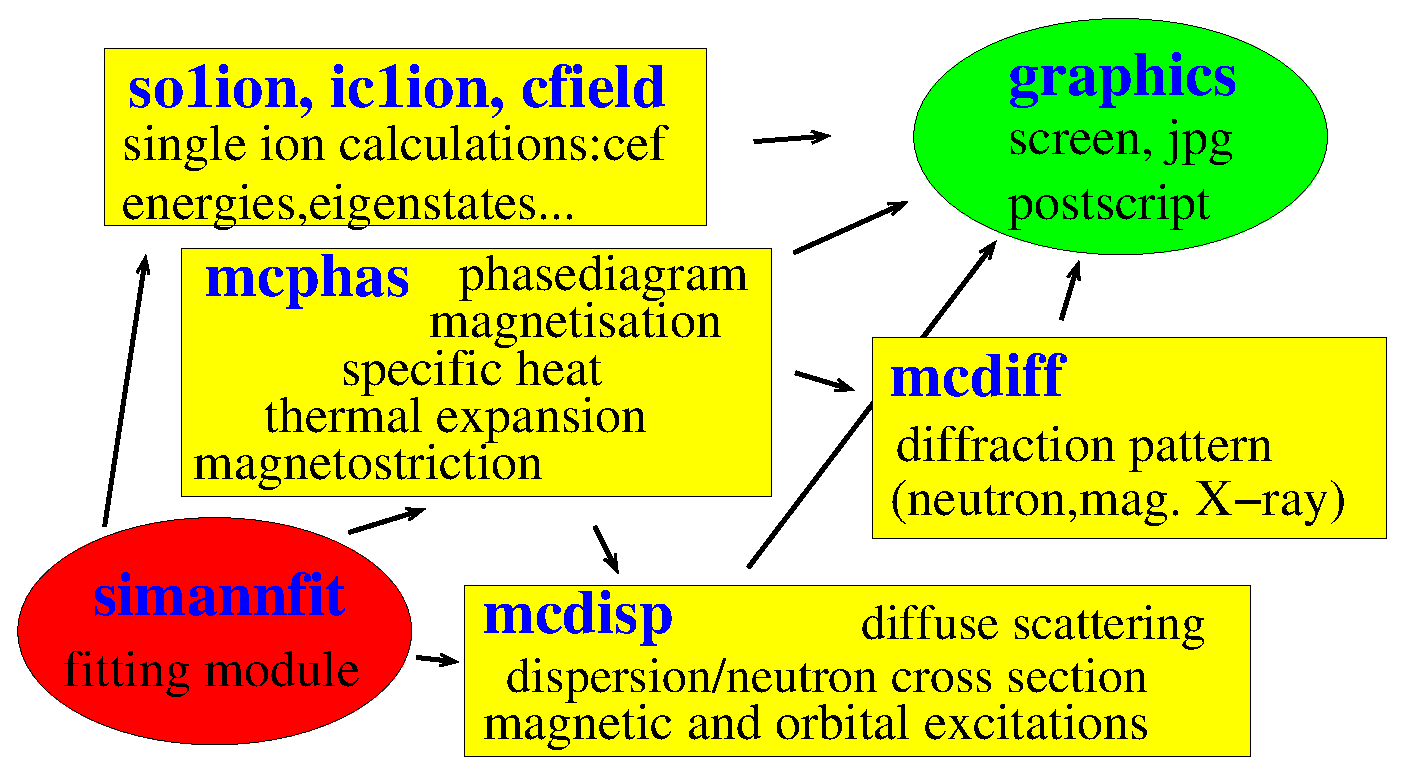
\includegraphics[angle=0,width=0.7\columnwidth]{figsrc/mcphas_modules.eps}
\caption{\label{modules}
Structure of the program package showing the tasks of the different modules.}
\end{center}
\end{figure}

\begin{description}
\item[so1ion(cfield):]
The best way to start with the program package is probably to get
acquainted with
the module {\prg so1ion\index{so1ion}}, which is the most important of several 
modules used for the calculation of single ion properties (see Section~\ref{cfield}).
\item[ic1ion:]
An advanced single ion module for intermediate coupling calcuations.
\item[mcphas:]
This module has been written to calculate the thermodynamic properties.
In order to  deal with the pair interactions a
 combined mean-field/monte-carlo algorithm is used in module {\prg mcphas}.
For a given temperature $T$ and magnetic field $\mbf H$ (vector)
 several possible magnetic structures are stabilised
by a mean field algorithm and the free energy is 
calculated. The initial values for this mean-field procedure are
modified by a Monte Carlo process.
See Section~\ref{runmcphas} on how to perform such a simulation.


The temperature and magnetic field is varied during the calculation
and thereby it is possible to map out the magnetic phase diagram.
The program produces a plot of the stabilised magnetic
structures and the magnetisation on screen, the
output files contain additional information 
such as calculated magnetoelastic and  neutron-diffraction
data. As a typical application of {\prg mcphas} the calculated magnetic
phase diagram of NdCu$_2$ is shown in fig.~\ref{ndphased}.
The exchange parameters required for the calculation of such a complex
antiferromagnet have
been determined from the dispersion of magnetic excitations
measured by neutron spectroscopy with moments aligned ferromagnetically
by an external magnetic field. Details are described elsewhere \cite{rotter00-29}.

\item[graphics:]
Several graphic programs easy the visualisation of the
calculated data (section~\ref{graphics}).

\item[mcdiff\index{mcdiff}:]
The module {\prg McDiff} can be used to calculate the magnetic neutrons
or resonant x-ray diffraction intensities. Note that neutron intensities
can be calculated going beyond the dipolar approximation for the magnetic
formfactor.

\item[mcdisp:]
An additional module {\prg McDisp} can be used to calculate the 
dispersion and intensity
 of magnetic excitations and diffuse magnetic scattering cross section.
  It is based on a mean field- random
phase approximation treatment of the problem (section~\ref{mcdisp}). 
\item[simannfit:]
In oder to enable the determination of the parameters of the
magnetic Hamiltonian from experimental data, a fitting module
{\prg Simannfit} can be used to fit experimental  magnetic structure and excitation
data. This module is based on the simulated annealing 
algorithm~\cite{kirkpatrick83-671} and described in section~\ref{simannfit}.
\end{description}

\begin{figure}[ht]\begin{center}
\includegraphics[angle=90,width=0.7\columnwidth]{figsrc/ndphased.ps}
\caption{\label{ndphased}
Magnetic phase diagram for NdCu$_2$ for magnetic field along
the orthorhombic $b$-direction. Colours represent the calculated phase
diagram, lines correspond to experimentally determined phase boundaries.
[plot created by program {\prg phased}]
}
\end{center}
\end{figure}


\section{Getting Started ...}  

First some important notes .... this manual does neither give an introduction into the theory of 
magnetism nor a description of the experimental techniques. In order
to use the program successfully, some basic knowledge of crystal field theory and the mean field
approximation is required, see for instance~\cite{jensen91-1}.
In order to compare the output of the calculation with experimental
data, it is recommended to be familiar with  experimental techniques used
in the investigation of magnetic properties
such as magnetisation, susceptibility, specific heat, magnetostriction
measurements and neutron scattering.

Using {\prg McPhase} for the first time, the reader should
\begin{itemize}
\item
rush into the program and test that it functions correctly on his system
by starting the demos ( type {\prg cd demo} and then run {\prg 01\_demo\_crystal\_fields.bat},{\prg %%@
02\_demo\_mcphas\_I\_NdCu2.bat}, etc.).  
\item 
learn about some special features and basic functions of the program package by
doing the tutorial in directory {\prg tutorial}
\item
look at the example calculations in directory {\prg examples}. These examples cover a large variety
of problems, which the program package may be applied to (see table~\ref{examples}). In addition, this directory
contains a large number of single ion property files which will be useful for setting
up numerical calculations for a specific system.
\item
with the help of this manual, which contains also some exercises the user is advised 
to learn about all details required to do a successful simulation of atomic magnetic properties
and set up calculations, which hopefully will be useful to interpret a large variety of 
experimental data. 
\end{itemize}

\begin{table}[thb] 
\begin{center}  
\caption {Description of the example calculations, which come along with the program package {\prg McPhase} in directory {\prg %%@
examples}:}   
\label{examples}   
\begin{tabular} 
{l|l|l|l}
compound & problem & single ion & references \\ 
        &          & module  &             \\
\hline
CeCu$_2$  & mag phase diagram, fit of dispersive mag. excitations to neutron data & {\prg kramer}\index{kramer} & %%@
\cite{loewenhaupt06-775,schedler03-1313} \\
CePd$_2$Si$_2$ & neutron diffraction going beyond dipolar approx for mag. formfactor & {\prg %%@
so1ion}&\cite{rotter09-140405} \\
CoO & magnetic formfactor - flipping ratios  and  highly inelastic neutron scattering  &{\prg  ic1ion} & \\
DyCu$_2$ & quadrupolar order and phase diagram & {\prg cfield}\index{cfield}&\cite{yoshida98-1421} \\
DyNi$_2$B$_2$C & magnetic phase diagram, special single ion module (quasiquartet) & {\prg %%@
quartett.so}\index{quartett.so}& \\
ErNi$_2$B$_2$C & magnetostriction and phase diagram & {\prg cfield}&\cite{doerr02-5609}\\
Gd$_3$GaO$_6$  & pointcharge model calculation of crystal field parameters & & \\ 
GdNi$_2$B$_2$C & magnetostriction and phase diagram, spin only (L=0) & {\prg brillouin}\index{brillouin}& \cite{doerr02-5609}\\
GdRu$_2$Si$_2$ & biquadratic interactions - magnetisation, magnetic structure & {\prg cfield} & \\
helix\_spinwave & spinwave calculation for a helical magnetic structure & {\prg so1ion} & \\
Ho$_2$Ti$_2$O$_7$ & diffuse magnetic scattering & {\prg so1ion} & \cite{bramwell01-1495}\\
LaSrCoO$_3$ & spin polarons quasielastic scattering & {\prg cluster}\index{cluster} & \cite{podlesnyak11-134430,podlesnyak08-247603} \\
La$_2$CoO$_4$ & dispersive magnetic excitations / spinwaves &{\prg  ic1ion} & \cite{lewtas10-184420}\\
LuMnO$_3$ &  magnetic structure and dispersion of excitations & {\prg so1ion} & \cite{lewtas10-184420} \\
NdBa$_2$Cu$_3$O$_7$ & fit of magnetic neutron diffraction data going beyond dipapprox & {\prg cfield}\index{cfield} & \cite{rotter09-140405} \\
NdCu$_2$  & crystal field, magnetic structure, phase diagrams, excitations & {\prg cfield}& %%@
\cite{loewenhaupt95-491,loewenhaupt96-499,rotter00-29,rotter02-751,rotter02-8885} \\
NiO            & INS and RIXS on NiO & {\prg so1ion}\index{so1ion} & \\
PrNi$_2$B$_2$C & crystal field - fit to neutrons,cp, susc & {\prg cfield}&\cite{mazumdar08-144422}\\
PrNi$_2$Si$_2$ & excitons in an amplitude modulated mag structure & {\prg so1ion}\index{so1ion} & \cite{blanco13-104411} \\
Pr$_3$Pd$_{20}$Si$_6$ & hyperfine interactions & {\prg cluster}\index{cluster} & \\
PuPd$_3$ & susceptibility, heat capacity & {\prg ic1ion}\index{ic1ion} & \cite{le10-155136} \\
TbCu$_2$ & magnetic phases with field parallel $a$ & {\prg cfield} \\
testic1ion & Pr$^{3+}$ chargedensity in IC and LS coupling & {\prg ic1ion,cfield} &\\
tungsten\_phonons & phonons in tungsten & {\prg phonon} & \\
UPd$_3$ & dispersive CEF excitations, quadrupolar interactions  & {\prg so1ion}\index{so1ion} & \cite{le12-036002} \\
 \end{tabular}
\end{center}   
\end{table}



Some publications referencing Mcstas: %%@
\cite{rotter02-751,rotter02-8885,rotter03-144418,rotter03-mass,rotter03-x,rotter04-231,rotter04-xxxx}



\clearpage
\section{The Hamiltonian}
\label{hamiltonian}

We assume a quantum mechanical system that can be described by the Hamiltonian
 \begin{equation}\label{hamilton}
 \hat \mathcal H=\sum_{n=1}^N \hat \mathcal H(n) -\frac{1}{2} \sum_{n,n',\alpha,\beta}
 {\mathcal J}_{\alpha\beta}(\mbf R_{n'} - \mbf R_n) \hat \mathcal I_{\alpha}^n \hat \mathcal I_{\beta}^{n'}.
 \end{equation}
The first term $\hat \mathcal H(n)$ denotes the Hamiltonian of
 a subsystem $n$
(e.g.~an ion, or cluster of ions). The second term describes a bilinear interaction 
between different subsystems
through the operators $\hat \mathcal I_{\alpha}^n$, with $\alpha = 1,2,...,m$. The operators $\hat \mathcal H(n)$ and $\hat \mathcal I_{\alpha}^n$  act in the subspace $n$ of the Hilbert space, i.e. $[\hat \mathcal I_{\alpha}^n,\hat \mathcal I_{\alpha}^{n'}]=0$,
$[\hat \mathcal H(n),\hat \mathcal I_{\alpha}^{n'}]=0$ and $[\hat \mathcal H(n),\hat \mathcal H(n')]=0$
for $n \neq n'$\footnote{Note that these conditions are essential and put a  limit to the
applicability of the theory, for example in the case of charge transfer excitations from
one subsystem to the next.}.
For example, in the case of a Heisenberg
 exchange between magnetic ions we would identify the set of operators with
 $\alpha=1,2,3$ with the three components of the  spin: $\hat \mathcal I_1 \leftrightarrow \hat S_x, \hat \mathcal I_2 %%@
\leftrightarrow \hat S_y, \hat \mathcal I_3 \leftrightarrow \hat S_z$.
The beauty of the analysis which follows is that it can be applied to
almost any Hamiltonian of the form (\ref{hamilton}). The analysis
of complex magnetic systems can thus be attempted by starting from a simple
form such as the Heisenberg model and by introducing, step-by-step, more
complexity into the model. For example, anisotropy and interactions with extended range can be introduced by modifying ${\mathcal J}_{\alpha\beta}(\mbf R_n - \mbf R_{n'})$, higher order operators can be 
introduced  by extending the index range for $\alpha$, and a complex single-ion term $\hat \mathcal H(n)$ may be added. 
Another example for a Hamiltonian (\ref{hamilton})  is the problem of lattice dynamics, which can
 be treated in the framework of this
formalism by identifying the operators $\hat \mathcal I^n_{\alpha}$
 with the atomic displacements $u^{n}$. Here the index $\alpha$ is not necessary and
$n$ refers to both, the atomic position index and the spatial coordinate of the displacement,
  $n=(1,x),(1,y),(1,z),(2,x),(2,y),(2,z), ...$. Note that this can be done, because the three spatial components of the 
displacement operators commute with each other (in contrast to the components of the spin) and each displacement
component acts in its own subspace of the Hilbert space. The kinetic energy
will be part of the single ion term $ \hat \mathcal H(n)$. Allowing more complexity to the system,
both the spin and lattice degrees of freedom can be introduced and spin-phonon interactions can be
handled by the theory.

The main limitation of the approach is that it neglects fluctuations associated with phase 
transitions and quantum disorder. We are primarily concerned, therefore, with excitations 
associated with a  well-ordered ground state.

Two special forms of the Hamiltonian (\ref{hamilton}), which have been implemented
are given in the following. Some other forms are also available, by programming
a single ion module the user may treat any type single ion Hamiltonian $\hat \mathcal H(n)$.


\subsection{Rare Earth Ions}

A more specific example of is the following magnetic  Hamiltonian $\mathcal H$ for rare earth ions,
 which may be treated with the program package:

\begin{equation}
\label{hamiltonre}
 {\mathcal H}= \sum_{n,lm} B_l^m O_{lm}({\mbf J}^n) 
             -\frac{1}{2}  \sum_{nn'} {\mathcal J}(nn') {\mbf J}^n{\mbf J}^{n'}
	     - \sum_{n} g_{Jn} \mu_B {\mbf J}^n {\mbf H} 
\end{equation}

The first term describes the crystal field (Stevens Operators $O_l^m$, see table in appendix~\ref{stevens}), the second %%@
the magnetic
exchange interaction, the third the Zeeman energy if an external magnetic field is applied.
Instead (or rather in addition) to this it is also possible to treat the 
more general two ion exchange coupling

\begin{equation}
\label{multipolehamilton}
 {\mathcal H}_{JJ}=
             -\frac{1}{2}  \sum_{nn'} \sum_ {ll'} \sum_{mm'}
	     {\mathcal K}_{ll'}^{mm'}(nn') O_{lm}({\mbf J}^n) O_{l'm'}({\mbf J}^{n'})
\end{equation}

For further information on the notation and symmetry restrictions to the
parameters in the Hamiltonian refer to~\cite{jensen91-1}.

In addition to the above terms in the Hamiltonian the coupling of magnetic and lattice properties
is possible by introducing magnetoelastic interactions:
In order to calculate magnetoelastic effects the parameters $B_l^m$, ${\mathcal J}(ij)$ (or more general
the ${\mathcal K}_{ll'}^{mm'}(ij)$) are expanded in a Taylor expansion in the strain tensor
$\epsilon$ resulting in the magnetoelastic interaction (i.e. keeping only the terms linear
in $\epsilon$). The equilibrium strain can be 
calculated by considering in addition the elastic energy and minimising the total free energy.
The procedure is described in detail in~\cite{rotter02-8885}.


 


\vspace{1cm}

{\em Exercises:}
\begin{itemize}
\item Write down the list of nonzero crystal field parameters in the crystal field Hamiltonian
of a Nd$^{3+}$ ion in an orthorhombic crystal field (Section~\ref{cfield} describes how such a parameter set
enters a {\prg McPhase} calculation).
\item Taking a primitive orthorhombic lattice of Nd$^{3+}$ ions write down the most general
anisotropic bilinear interaction  for the nearest neighbour exchange interaction
(Section~\ref{mcphasj} describes how such a parameters set enters a {\prg McPhase calculation}).
\end{itemize}

%The $\tilde O_l^m$ in are the Racah  operators, which form a set of irreducible
%tensor operators.

\subsection{Intermediate Coupling}

For some rare earth ions and for transition metals or actinides it is necessary to
include more singleion ion states with differen L,S into the calculation. This
can be done in intermediate coupling using the module {\prg ic1ion}\index{ic1ion}, which
explicitely includes electrostatic and  spin orbit interactions for each ion:

\begin{eqnarray}
\label{ichamilton}
 {\mathcal H}&=& \sum_n \left \{ \sum_{i_n=1}^{\nu_n}
 \left [ \frac{p_{i_n}^2}{2m_e}
        -\frac{Z_n e^2}{4\pi\epsilon_0|\mbf r_{i_n}-\mbf R_n|}
        +\zeta_n  \mbf l^{i_n} \cdot \mbf s^{i_n}
        + \sum_{lm} L_l^m(n) T_{lm}^n
\right ]
              + \sum_{i_n>j_n=1}^{\nu_n}\frac{e^2}{4\pi\epsilon_0|\mbf r_{i_n}-\mbf r_{j_n}|} \right \} \nonumber \\
	    && - \sum_{n}  \mu_B (2\mbf S^n+\mbf L^n) {\mbf H}  \nonumber\\
            && -\frac{1}{2} \sum_{nn'} \left[ 
({\hat \mbf L}^n,{\hat \mbf S}^n )
\stackrel{=}{\mathcal J}(nn') 
\left ( \begin{array}{c} {\hat \mbf L}^{n'} \\
        {\hat \mbf S}^{n'} \end{array}
\right )
     + \sum_{kk'} \sum_{qq'}  \mathcal{K}_{kk'}^{qq'}(nn') \hat{T}_{kq}^n T_{k'q'}^{n'} \right]
\end{eqnarray}

Here $\nu_n$,$Z_n$ and $\mbf R_n$ denote the number of electrons, the charge of the nucleus
and the position
 of the ion number $n$,respectively, for each electron being
$p$ the momentum, $m_e$ the mass, $e$ the charge and $\mbf r$ the location.
Spin orbit coupling is written in terms of the orbital momentum $\mbf l$ and
spin $\mbf s$ of the individual electrons. The
 Zeman interaction and two ion interaction are written in terms of 
the (inverse) total spin $\mbf S_n$ and (inverse) total orbital momentum $\mbf L_n$
of ion number $n$. The crystal field in intermediate coupling is written
in terms of Wybourne parameters $L_l^m$ and Wybourne operators $T_{lm}^n$, operator equivalents
of real valued 
spherical harmonic functions 
$T_{l0}=\sqrt{4\pi/(2l+1)}\sum_iY_{l0}(\Omega_{i_n})$, 
$T_{l,\pm|m|}=\sqrt{4\pi/(2l+1)}\sum_i \sqrt{\pm1}[Y_{l,-|m|}(\Omega_{i_n})\pm (-1)^m Y_{l,|m|}(\Omega_{i_n})]$ for the ion $n$,
for details on crystal field parameter 
conventions see appendix~\ref{cfparconventions}.

\clearpage

\section{{\prg so1ion}\index{so1ion} ({\prg cfield}\index{cfield}) - a crystal field module for rare earth %%@
ions (calculate energy levels, transition matrix elements)}\label{cfield}

\subsection{Using {\prg so1ion} ({\prg Cfield}) separately}
\label{cfieldsep}

The crystal field is the electrostatic field, which is produced by the
charges of the crystal environment of a rare earth atom. It acts on the
4f electrons of the rare earth and causes magnetic anisotropy. Fig.~\ref{chrgpla} and
\ref{chrgplb} show the effect of this field on the charge distribution.
Such plots can be made by using the programs {\prg pointc\index{pointc}} to calculate
the crystal field parameters and
 {\prg chrgplt\index{chrgplt}} to plot the charge density, see section \ref{addprog}.

\begin{figure}[hb]
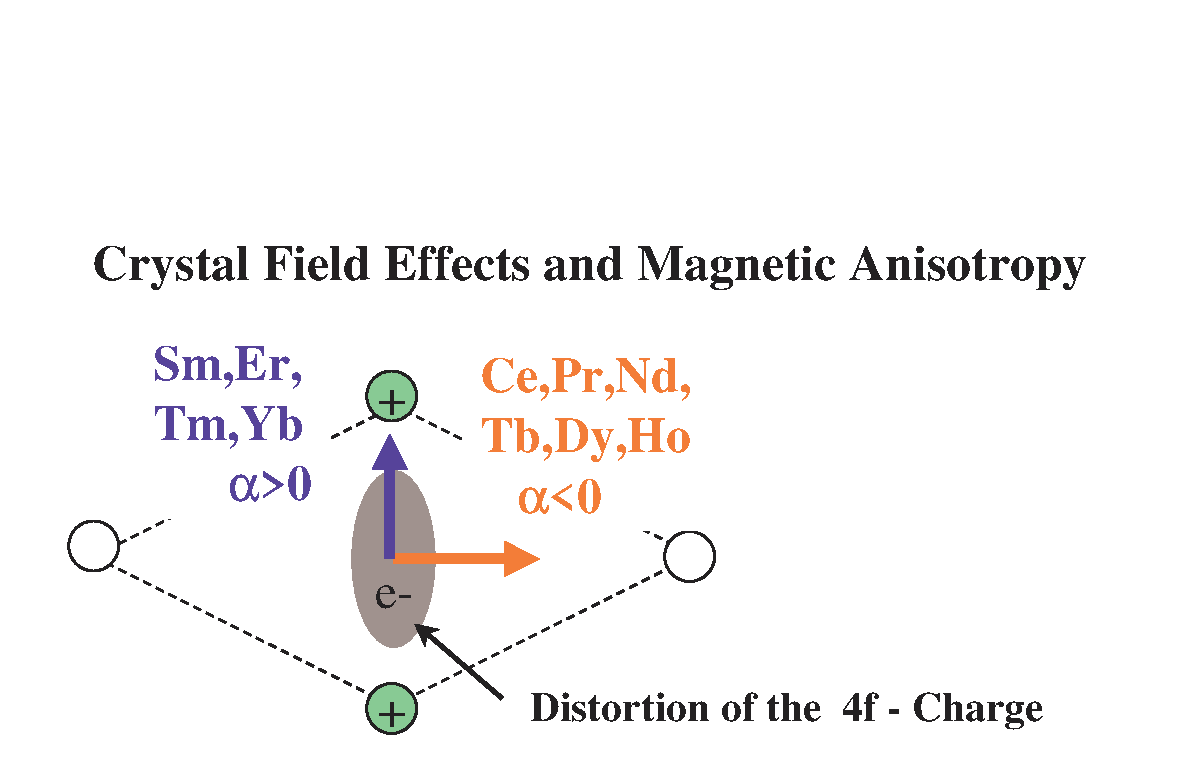
\includegraphics[angle=0,width=0.7\columnwidth]{./figsrc/crystalfieldplot.eps}
\caption{\label{chrgpla}
The crystal field model: the figure shows the influence of two positive 
charges on the charge density of 4f-electrons. The
charge density is distorted by the electric field from the neighbouring atoms.
Furthermore, this distortion leads to an anisotropy of the magnetic properties
of the 4f shell. The resulting 
easy direction of the magnetic moment is shown by arrows for the different tri positive
rare earth ions.} 
\end{figure}

\begin{figure}[ht]
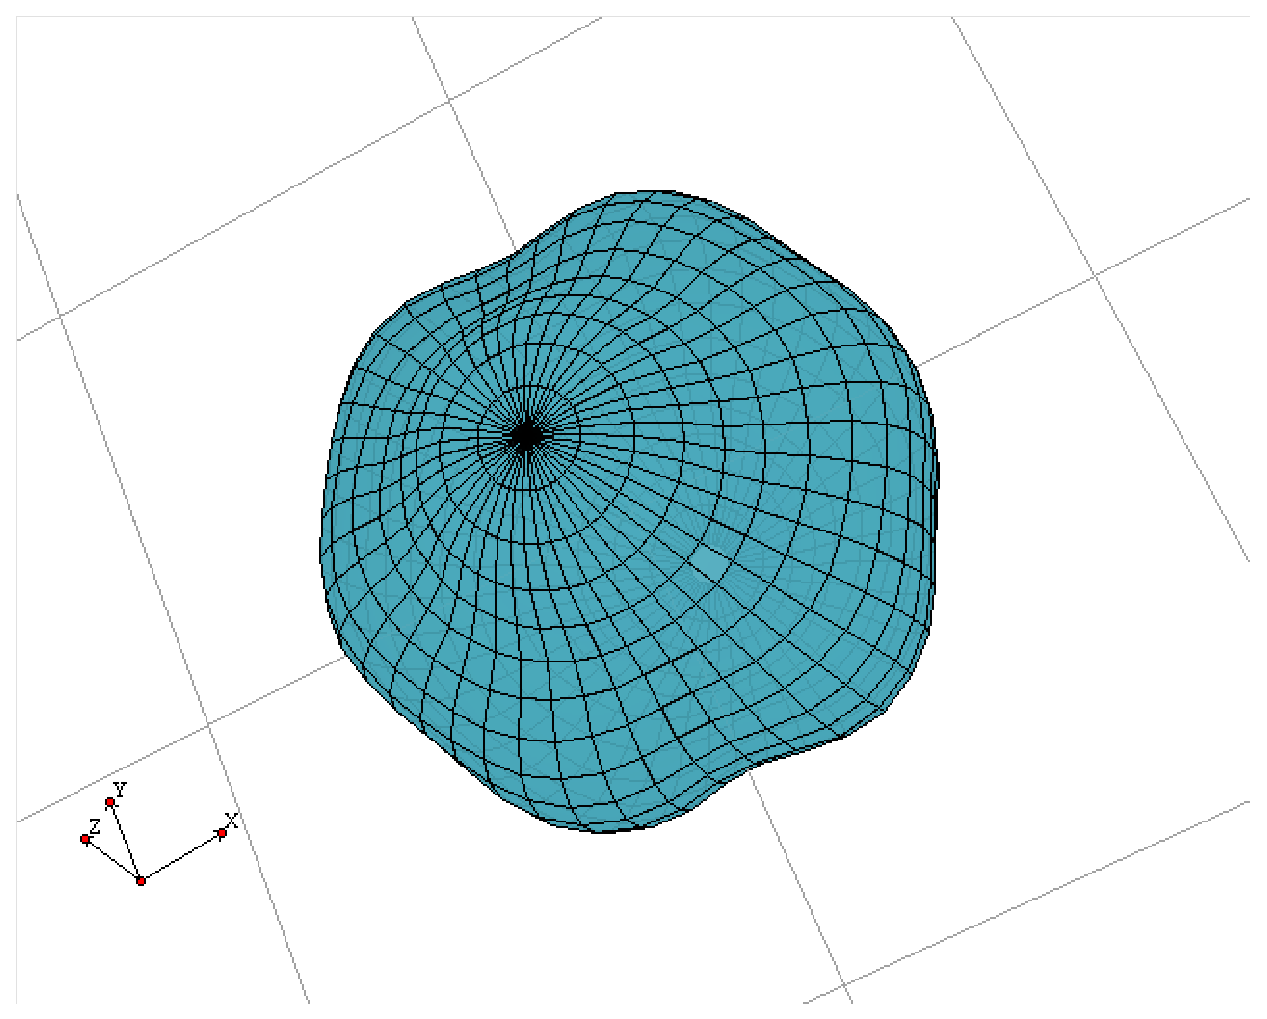
\includegraphics[angle=0,width=0.7\columnwidth]{./figsrc/chrgpla.eps}
\caption{\label{chrgplb}
Calculated charge density of 4f-electrons in an orthorhombic crystal field. In
this example the charge density of a Nd$^{3+}$ ion at a temperature of 10~K was 
calculated by taking the crystal
field parameters determined by neutron spectroscopy and 
magnetic measurements in NdCu$_2$~\cite{gratz91-9297}.
[plot created by program {\prg chrgplt\index{chrgplt}+javaview}]}
\end{figure}

We will describe now, how the crystal field influence can be quantitatively evaluated
and how {\prg so1ion}\index{so1ion}  can help to do this.
Within the $|JLSm_J \rangle$ ground state multiplet of the 4f electron wave function 
the crystal field can be described by the following Hamiltonian:

\begin{equation}
\label{cfham}
 {\mathcal H}= \sum_{s,lm} B_{lm} O_{lm}({\mbf J}^s) 
	     - \sum_{s} g_{Js} \mu_B {\mbf J}^s {\mbf H} 
\end{equation}

The first term in equ.~\ref{cfham} describes the crystal field, the second the
effect of a magnetic field (Zeeman term). The strength of the crystal field is given by the
crystal field parameters $B_l^m$. In the case of isolating materials these
parameters can be obtained by the point charge model (point charges on the 
neighbouring atoms, for details on these calculations see~\cite{hutchings64-227},
in the {\prg McPhase} suite use programs {\prg makenn} and {\prg pointc} to evaluate
the pointcharge model for a given crystal structure, see section~\ref{addprog}).
For metals the conduction electrons screen the point charges and the determination
of the crystal field is usually only possible by fits to experimental data. 
The program package {\prg McPhase} may be used to solve such crystal field problems.

A simpler way of dealing with crystal field anisotropy is to write
instead of the first term in equ.~\ref{cfham}

\begin{equation}
  \sum_s D_x^2 (J_x^s)^2 + D_y^2 (J_y^s)^2 +D_z^2 (J_z^s)^2 
\end{equation}

In order to implement a full diagonalisation of the single ion crystal field Hamiltonian
the module {\prg so1ion}\index{so1ion}({\prg cfield\index{cfield}}, written by P. Fabi n\'e Hoffmann) has %%@
been included into the program package. It  can be used separately to 
calculate crystal field problems. The program is self explaining, provided 
the user has a basic knowledge of crystal field 
theory (see e.g. the famous article by Hutchings~\cite{hutchings64-227}).
The program is started by typing {\prg so1ion}\index{so1ion} and displays help messages. 

\subsection{Example - how to evaluate the crystal field of NdCu$_2$ using {\prg %%@
so1ion}\index{so1ion}}\label{cfieldexample}

All the files described in the following procedure are available in the directory
{\prg examples/ndcu2b\_new/cf}.

A simple input file is made up in the following:

\begin{itemize}
\item The first line in the input file tells {\prg so1ion}\index{so1ion} that it should use simple input %%@
format.
\item Comment lines start with \#. 
\item The type of ion has to be given plus
several lines containing the crystal field parameters. 
\end{itemize}

It follows an example, we take the values
for NdCu$_2$ from literature~\cite{gratz91-9297}. Note that
if the crystal field parameters are not known, there are different
possibilities to obtain values, such as ab initio calculation,
point charge calculations (use module {\prg pointc\index{pointc}}) and fitting
to experimental data (see section~\ref{simannfit}).

\begin{verbatim}
#!MODULE=so1ion
#<!--mcphas.cf-->
# comment followed by
# the ion type and the crystal field parameters [meV]
 IONTYPE=Nd3+
# - note you can also do any pure spin problem by entering e.g. IONTYPE=S=2.5 
 B20=  0.116765                                           
 B22  =  0.134172                                           
 B40  =  0.0019225                                          
 B42  =  0.0008704                                          
 B44  =  0.0016916                                          
 B60  =  0.0000476                                          
 B62  =  0.0000116                                          
 B64  =  0.0000421                                          
 B66  =  0.0003662       
# instead of the Stevens parameters Blm 
# second order crystal field parameters Dx^2 Dy^2 and Dz^2 can be entered in meV
Dx2=0.1
Dy2=0
Dz2=0.4
# the temperature in Kelvin
TEMP= 10
# if you want you can apply a magnetic field in Tesla
Bx=0
By=0
Bz=0
\end{verbatim}

Note: you can also create an input file for so1ion with more comments for the crystal field
parameters, the type of ion etc. This is done by running {\prg so1ion}\index{so1ion} with the
option {\em -c}, i.e.: {\bf so1ion -c}, a help screen appears ...

\begin{enumerate} 
\item
The calculation of the single ion properties is 
performed using {\prg so1ion}\index{so1ion} with the option {\prg -r}, 
i.e. type the command {\bf so1ion -r filename -B} where filename
refers to the name of the single ion property file.
Files
{\prg so1ion.out} and {\prg levels.cef} (short summary, usable as input for
{\prg mcdiff\index{mcdiff}}) are generated, which contain the results of the calculation, i.e.
the diagonalisation of the Hamilton operator and the neutron scattering cross section.
The program {\prg so1ion}\index{so1ion} outputs a variety of results, such as eigenvectors and 
energies of the crystal field states. In addition it provides 
the total neutron powder cross section for each crystal field
transitions (in barn/ion) at a given temperature according to the formula

\begin{equation}
\sigma(i\rightarrow k)=4\pi \left(\frac{\hbar \gamma e^2}{mc^2}\right)^2
\frac{exp(-E_i/k_BT)}{\sum_j exp(-E_j/k_BT)} \frac{2}{3}\sum_{\alpha=x,y,z}
|\langle i|J^{\alpha}|k\rangle|^2
\end{equation}

Note: in this calculation energy and Q dependence
of the double differential scattering cross section are not considered and
integration over all energies and scattering angles has been performed.
In order to get a more realistic scattering intensity, the
form factor (giving a $Q$ dependence), the
factor $k'/k$ and the Debye Waller factor $exp(-W(Q))$ should be considered.

Here comes the output file {\prg so1ion.out}:
{\footnotesize
\begin{verbatim}
#{VERSION :   5.40      |
#-------------------------------------------------------------- 
#                   C F I E L D / S O 1 I O N                  |
#                    A crystal field program                   |
#               __________________________________              
#              |         Peter  Hoffmann          |             
#              |    Forschungszentrum Juelich     |             
#              |Institut fuer Festkoerperforschung|             
#              |Tel.: 02461-616896                |             
#               __________________________________              
#                          O U T P U T                         
#-------------------------------------------------------------- 
#!Temperature of the sample       T=   2.00 Kelvin                
#!Ion                    IONTYPE= Nd3+                          
#!Lande factor of the ion   gJ= 0.727273                       
#                                                              
# Total angular momentum J of the                               
#!Spin - orbit - level     J=  4.5                            
#!Electrons in 4f shell   Ne=  3                              
#  local point symmetry                                        
#! of the ion              PS= triklin                               
#! Symmetry_number            = 0                              
#-------------------------------------------------------------- 
# Parameter           :  Akq   in  meV   /a0**k                  
# (compare Hutchings p 255 eq 5.5)                             
#!A20  =        -16.306372                                     
#!A22  =        -18.737280                                     
#                                                              
#!A40  =         -2.269445                                     
#!A42  =         -1.027477                                     
#!A44  =         -1.996875                                     
#                                                              
#!A60  =         -0.083369                                     
#!A62  =         -0.020317                                     
#!A64  =         -0.073736                                     
#!A66  =         -0.641377                                     
#-------------------------------------------------------------- 
#-------------------------------------------------------------- 
# Parameter           :  Bkq   in  meV                           
#                        (Stevens Parameters comp Hutchings)
#!B20  =          0.116765                                     
#!B22  =          0.134172                                     
#                                                              
#!B40  =          0.001922                                     
#!B42  =          0.000870                                     
#!B44  =          0.001692                                     
#                                                              
#!B60  =          0.000048                                     
#!B62  =          0.000012                                     
#!B64  =          0.000042                                     
#!B66  =          0.000366                                     
#-------------------------------------------------------------- 
#-------------------------------------------------------------- 
# Parameter           :  Dkq   in  meV                           
#!D20 =         -36.330596                                     
#!D22 =         -17.043002                                     
#                                                              
#!D40 =         -52.832675                                     
#!D42 =          -3.782031                                     
#!D44 =          -5.556290                                     
#                                                              
#!D60 =         -20.048458                                     
#!D62 =          -0.476801                                     
#!D64 =          -1.579686                                     
#!D66 =         -10.148138                                     
#-------------------------------------------------------------- 
#-------------------------------------------------------------- 
# Parameter           :  Lkq   in  meV                           
#                        (Wyborne Parameters comp Kassmann)
#!L20  =        -36.330596                                     
#!L22  =        -17.043002                                     
#                                                              
#!L40  =        -52.832675                                     
#!L42  =         -3.782031                                     
#!L44  =         -5.556290                                     
#                                                              
#!L60  =        -20.048458                                     
#!L62  =         -0.476801                                     
#!L64  =         -1.579686                                     
#!L66  =        -10.148138                                     
#-------------------------------------------------------------- 
#-------------------------------------------------------------- 
# Parameter           :  Vkq   in  meV                           
# (NOT the same Vlm as in Hutchings p255 or Elliot and Stevens)
#!V20 =           0.116765                                     
#!V22 =           0.067086                                     
#                                                              
#!V40 =           0.001922                                     
#!V42 =           0.000435                                     
#!V44 =           0.000846                                     
#                                                              
#!V60 =           0.000048                                     
#!V62 =           0.000002                                     
#!V64 =           0.000021                                     
#!V66 =           0.000183                                     
#-------------------------------------------------------------- 
#-------------------------------------------------------------- 
# Parameter           :  Wkq   in  meV   /a0**k                  
#!W20 =         -16.306372                                     
#!W22 =          -9.368640                                     
#                                                              
#!W40 =          -2.269445                                     
#!W42 =          -0.513739                                     
#!W44 =          -0.998438                                     
#                                                              
#!W60 =          -0.083369                                     
#!W62 =          -0.003386                                     
#!W64 =          -0.036868                                     
#!W66 =          -0.320689                                     
#-------------------------------------------------------------- 
#
#-------------------------------------------------------------- 
#                   Magnetic field B in Tesla .                    
#                                                              
#                   H = H   +  H       + H                     
#                        CF     mag_ex    mag_mol              
#                                                              
#--------------------------------------------------------------
#                                                              
#  H        = - g  my   J  B                                   
#   mag_ex       J   B  -  - ex                                
#                                                              
#--------------------------------------------------------------
#                                                              
#  H        = - 2 ( g - 1 ) my   J  B                          
#   mag_mol          J        B  -  - mol                      
#                                                              
#--------------------------------------------------------------
#                                                              
#! Bx_ex   =          0.00                                     
#! By_ex   =          0.00                                     
#! Bz_ex   =          3.00                                     
#                                                              
#! Bx_mol  =          0.00                                     
#! By_mol  =          0.00                                     
#! Bz_mol  =          0.00                                     
#                                                              
#                                                              
#-------------------------------------------------------------- 
#
#
#-------------------------------------------------------------- 
# Energy Eigenvalues are in  meV   .          	            
#--------------------------------------------------------------
#!Nr of different energy levels   noflevels=10                 
#!Energy shift   Eshift=                       -6.1829 
#                                                              
# Because of the calibration freedom the smallest energy       
# eigenvalue is shifted to zero. You can get the energy        
# eigen-value of the applied eigen-value problem               
# by shifting the energy by the added energy value above       
#!*E( 1)=        0.0000        Degeneracy =   1 -fold            
#!*E( 2)=        0.6253        Degeneracy =   1 -fold            
#!*E( 3)=        3.2216        Degeneracy =   1 -fold            
#!*E( 4)=        3.2555        Degeneracy =   1 -fold            
#!*E( 5)=        5.2391        Degeneracy =   1 -fold            
#!*E( 6)=        5.3833        Degeneracy =   1 -fold            
#!*E( 7)=        7.5859        Degeneracy =   1 -fold            
#!*E( 8)=        7.5951        Degeneracy =   1 -fold            
#!*E( 9)=       13.9267        Degeneracy =   1 -fold            
#! E(10)=       14.9961        Degeneracy =   1 -fold            
# Them with  *  marked Energy eigenvalues have a non-          
# vanishing Matrix element of the Ground state E( 1).          
#-------------------------------------------------------------- 
#
#-------------------------------------------------------------- 
# The orthonormal characteristic Eigenvectors  |i,r>  with     
#                                                              
#             H |i,r>  = ( E  + E      ) |i,r>  , r=1 ... n    
#                           i    shift                     i   
#                                                              
#                            and                               
#                                                              
#                    <i,r|j,s> = D   D                         
#                                 ij  rs                       
#                                                              
#              D  = Kronecker- Delta function                  
#               ij                                             
#                                                              
# the |i,r> are also orthonormal .                             
# We consider in this program  Crystal Field spliting          
# at the lowest Spin-orbit-level (Ground state)                
#                                                              
# 2S+1                                                         
#     L  of the calualted Ion. The |i,r> are in                
#      J                                                       
#                                                              
# a more developed  Eigenfunction   			    
#                                                              
# system  [ | J  M   > ]               ,where                  
#                 J     M = -J,...,J                           
#                        J                                     
#                               ,                              
#              <  J  M   |  J  M  >  =  D    ,    .            
#                     J         J        M  M                  
#                                         J  J                 
#--------------------------------------------------------------
#                                                              
# I 1, 1> =     0.0424               I 4.5  -4.5>              
#          -    0.3284               I 4.5  -2.5>              
#          +    0.0834               I 4.5  -0.5>              
#          -    0.2234               I 4.5   1.5>              
#          +    0.9130               I 4.5   3.5>              
#                                                              
# I 2, 1> =     0.8586               I 4.5  -3.5>              
#          -    0.2351               I 4.5  -1.5>              
#          +    0.1475               I 4.5   0.5>              
#          -    0.4274               I 4.5   2.5>              
#          +    0.0560               I 4.5   4.5>              
#                                                              
# I 3, 1> =     0.3625               I 4.5  -3.5>              
#          +    0.2363               I 4.5  -1.5>              
#          -    0.8490               I 4.5   0.5>              
#          +    0.3025               I 4.5   2.5>              
#          -    0.0207               I 4.5   4.5>              
#                                                              
# I 4, 1> =     0.0279               I 4.5  -4.5>              
#          -    0.2959               I 4.5  -2.5>              
#          +    0.8547               I 4.5  -0.5>              
#          -    0.3316               I 4.5   1.5>              
#          -    0.2669               I 4.5   3.5>              
#                                                              
# I 5, 1> =     0.1624               I 4.5  -3.5>              
#          -    0.6457               I 4.5  -1.5>              
#          +    0.1503               I 4.5   0.5>              
#          +    0.7305               I 4.5   2.5>              
#          -    0.0205               I 4.5   4.5>              
#                                                              
# I 6, 1> =     0.0010               I 4.5  -4.5>              
#          +    0.7060               I 4.5  -2.5>              
#          -    0.0029               I 4.5  -0.5>              
#          -    0.7034               I 4.5   1.5>              
#          +    0.0821               I 4.5   3.5>              
#                                                              
# I 7, 1> =     0.3206               I 4.5  -3.5>              
#          +    0.6617               I 4.5  -1.5>              
#          +    0.4732               I 4.5   0.5>              
#          +    0.4090               I 4.5   2.5>              
#          -    0.2610               I 4.5   4.5>              
#                                                              
# I 8, 1> =    -0.2262               I 4.5  -4.5>              
#          +    0.5337               I 4.5  -2.5>              
#          +    0.5046               I 4.5  -0.5>              
#          +    0.5676               I 4.5   1.5>              
#          +    0.2953               I 4.5   3.5>              
#                                                              
# I 9, 1> =     0.0482               I 4.5  -3.5>              
#          +    0.1844               I 4.5  -1.5>              
#          +    0.1046               I 4.5   0.5>              
#          +    0.1577               I 4.5   2.5>              
#          +    0.9633               I 4.5   4.5>              
#                                                              
# I10, 1> =     0.9728               I 4.5  -4.5>              
#          +    0.1462               I 4.5  -2.5>              
#          +    0.0892               I 4.5  -0.5>              
#          +    0.1520               I 4.5   1.5>              
#          +    0.0364               I 4.5   3.5>              
#                                                              
#-------------------------------------------------------------- 
#
#!magnetic moment(mb/f.u.): mx= 0.000 my= 0.000 mz= 1.880
#
#-------------------------------------------------------------- 
#                                                              
#                  M A T R I X  E L E M E N T                  
#                  S I N G L E  C R Y S T A L                    
#                                                              
#--------------------------------------------------------------
#    Only the marix elements that are non-zero are written     
#                                                              
#--------------------------------------------------------------
#                              2 |            2 |            2 
#    a  <-->  b      |<a|J |b>|  |  |<a|J |b>|  |  |<a|J |b>|  
#                         x      |       y      |       z      
#--------------------------------+--------------+--------------
#    1  <-->  1       0.000000   |   0.000000   |   7.349037   
#--------------------------------+--------------+--------------
#    2  <-->  1       0.837715   |   4.124524   |   0.000000   
#--------------------------------+--------------+--------------
#    2  <-->  2       0.000000   |   0.000000   |   4.757295   
#--------------------------------+--------------+--------------
#    3  <-->  1       0.097402   |   1.800867   |   0.000000   
#--------------------------------+--------------+--------------
#    3  <-->  2       0.000000   |   0.000000   |   1.951770   
#--------------------------------+--------------+--------------
#    3  <-->  3       0.000000   |   0.000000   |   0.002243   
#--------------------------------+--------------+--------------
#    4  <-->  1       0.000000   |   0.000000   |   1.052055   
#--------------------------------+--------------+--------------
#    4  <-->  2       0.006254   |   2.906196   |   0.000000   
#--------------------------------+--------------+--------------
#    4  <-->  3       1.883036   |   8.933883   |   0.000000   
#--------------------------------+--------------+--------------
#    4  <-->  4       0.000000   |   0.000000   |   0.030053   
#--------------------------------+--------------+--------------
#    5  <-->  1       1.296760   |   0.787532   |   0.000000   
#--------------------------------+--------------+--------------
#    5  <-->  2       0.000000   |   0.000000   |   2.221074   
#--------------------------------+--------------+--------------
#    5  <-->  3       0.000000   |   0.000000   |   0.263606   
#--------------------------------+--------------+--------------
#    5  <-->  4       3.031073   |   4.748191   |   0.000000   
#--------------------------------+--------------+--------------
#    5  <-->  5       0.000000   |   0.000000   |   0.396361   
#--------------------------------+--------------+--------------
#    6  <-->  1       0.000000   |   0.000000   |   1.160910   
#--------------------------------+--------------+--------------
#    6  <-->  2       1.453148   |   0.329358   |   0.000000   
#--------------------------------+--------------+--------------
#    6  <-->  3       3.692640   |   4.510482   |   0.000000   
#--------------------------------+--------------+--------------
#    6  <-->  4       0.000000   |   0.000000   |   0.634606   
#--------------------------------+--------------+--------------
#    6  <-->  5       4.539708   |   5.382444   |   0.000000   
#--------------------------------+--------------+--------------
#    6  <-->  6       0.000000   |   0.000000   |   0.230677   
#--------------------------------+--------------+--------------
#    7  <-->  1       0.284349   |   1.844604   |   0.000000   
#--------------------------------+--------------+--------------
#    7  <-->  2       0.000000   |   0.000000   |   1.435031   
#--------------------------------+--------------+--------------
#    7  <-->  3       0.000000   |   0.000000   |   0.258615   
#--------------------------------+--------------+--------------
#    7  <-->  4       0.926445   |   0.049897   |   0.000000   
#--------------------------------+--------------+--------------
#    7  <-->  5       0.000000   |   0.000000   |   1.601018   
#--------------------------------+--------------+--------------
#    7  <-->  6       0.005768   |   0.457608   |   0.000000   
#--------------------------------+--------------+--------------
#    7  <-->  7       0.000000   |   0.000000   |   0.032325   
#--------------------------------+--------------+--------------
#    8  <-->  1       0.000000   |   0.000000   |   1.472943   
#--------------------------------+--------------+--------------
#    8  <-->  2       0.119332   |   2.256706   |   0.000000   
#--------------------------------+--------------+--------------
#    8  <-->  3       0.711683   |   0.039222   |   0.000000   
#--------------------------------+--------------+--------------
#    8  <-->  4       0.000000   |   0.000000   |   0.122925   
#--------------------------------+--------------+--------------
#    8  <-->  5       0.091000   |   0.073150   |   0.000000   
#--------------------------------+--------------+--------------
#    8  <-->  6       0.000000   |   0.000000   |   2.114855   
#--------------------------------+--------------+--------------
#    8  <-->  7      14.237466   |   0.119658   |   0.000000   
#--------------------------------+--------------+--------------
#    8  <-->  8       0.000000   |   0.000000   |   0.078994   
#--------------------------------+--------------+--------------
#    9  <-->  1       1.853194   |   0.788092   |   0.000000   
#--------------------------------+--------------+--------------
#    9  <-->  2       0.000000   |   0.000000   |   0.000005   
#--------------------------------+--------------+--------------
#    9  <-->  3       0.000000   |   0.000000   |   0.020033   
#--------------------------------+--------------+--------------
#    9  <-->  4       0.046976   |   0.352198   |   0.000000   
#--------------------------------+--------------+--------------
#    9  <-->  5       0.000000   |   0.000000   |   0.128492   
#--------------------------------+--------------+--------------
#    9  <-->  6       0.005534   |   0.062238   |   0.000000   
#--------------------------------+--------------+--------------
#    9  <-->  7       0.000000   |   0.000000   |   1.398393   
#--------------------------------+--------------+--------------
#    9  <-->  8       2.221975   |   0.206978   |   0.000000   
#--------------------------------+--------------+--------------
#    9  <-->  9       0.000000   |   0.000000   |  17.505703   
#--------------------------------+--------------+--------------
#   10  <-->  1       0.000000   |   0.000000   |   0.000017   
#--------------------------------+--------------+--------------
#   10  <-->  2       1.649987   |   0.701605   |   0.000000   
#--------------------------------+--------------+--------------
#   10  <-->  3       0.149440   |   0.435077   |   0.000000   
#--------------------------------+--------------+--------------
#   10  <-->  4       0.000000   |   0.000000   |   0.026213   
#--------------------------------+--------------+--------------
#   10  <-->  5       0.104403   |   0.085187   |   0.000000   
#--------------------------------+--------------+--------------
#   10  <-->  6       0.000000   |   0.000000   |   0.170024   
#--------------------------------+--------------+--------------
#   10  <-->  7       1.869528   |   0.229295   |   0.000000   
#--------------------------------+--------------+--------------
#   10  <-->  8       0.000000   |   0.000000   |   0.883112   
#--------------------------------+--------------+--------------
#   10  <-->  9       0.135184   |   0.025006   |   0.000000   
#--------------------------------+--------------+--------------
#   10  <--> 10       0.000000   |   0.000000   |  18.285922   
#-------------------------------------------------------------- 
#
#
#-------------------------------------------------------------- 
#                                                              
#                  M A T R I X  E L E M E N T S                
#                    P O L Y C R Y S T A L                     
#                                                              
#--------------------------------------------------------------
#                                                              
#                             ----                2            
# Matrix element       :      >     |<i,r|J |k,s>|             
#                             ----         T                   
#                              r,s                             
#                                                              
#                                                              
# for the transition :      E  ->  E                           
#                              i      k                        
#                                                              
#--------------------------------------------------------------
#                                                              
#                         SUm rule :                           
#                                                              
#             ----                2       2                    
#             >     |<i,r|J |k,s>|  = n  --- J(J+1)            
#             ----         T           i  3                    
#             k,r,s                                            
#-------------------------------------------------------------- 
#------------------------------------------------- 
# \ E |   |   |   |   |   |   |   |   |   |   |Zei|
#E \ k|E  |E  |E  |E  |E  |E  |E  |E  |E  |E  |len|
# i \ | 1 | 2 | 3 | 4 | 5 | 6 | 7 | 8 | 9 | 10|sum|
#----|---|---|---|---|---|---|---|---|---|---|---|
#| E  |  4|  3|  1|   |  1|   |  1|   |  1|   | 16|
#|  1 |.90|.31|.27|.70|.39|.77|.42|.98|.76|   |.50|
#|----|---|---|---|---|---|---|---|---|---|---|---|
#| E  |  3|  3|  1|  1|  1|  1|   |  1|   |  1| 16|
#|  2 |.31|.17|.30|.94|.48|.19|.96|.58|   |.57|.50|
#|----|---|---|---|---|---|---|---|---|---|---|---|
#| E  |  1|  1|   |  7|   |  5|   |   |   |   | 16|
#|  3 |.27|.30|   |.21|.18|.47|.17|.50|.01|.39|.50|
#|----|---|---|---|---|---|---|---|---|---|---|---|
#| E  |   |  1|  7|   |  5|   |   |   |   |   | 16|
#|  4 |.70|.94|.21|.02|.19|.42|.65|.08|.27|.02|.50|
#|----|---|---|---|---|---|---|---|---|---|---|---|
#| E  |  1|  1|   |  5|   |  6|  1|   |   |   | 16|
#|  5 |.39|.48|.18|.19|.26|.61|.07|.11|.09|.13|.50|
#|----|---|---|---|---|---|---|---|---|---|---|---|
#| E  |   |  1|  5|   |  6|   |   |  1|   |   | 16|
#|  6 |.77|.19|.47|.42|.61|.15|.31|.41|.05|.11|.50|
#|----|---|---|---|---|---|---|---|---|---|---|---|
#| E  |  1|   |   |   |  1|   |   |  9|   |  1| 16|
#|  7 |.42|.96|.17|.65|.07|.31|.02|.57|.93|.40|.50|
#|----|---|---|---|---|---|---|---|---|---|---|---|
#| E  |   |  1|   |   |   |  1|  9|   |  1|   | 16|
#|  8 |.98|.58|.50|.08|.11|.41|.57|.05|.62|.59|.50|
#|----|---|---|---|---|---|---|---|---|---|---|---|
#| E  |  1|   |   |   |   |   |   |  1| 11|   | 16|
#|  9 |.76|   |.01|.27|.09|.05|.93|.62|.67|.11|.50|
#|----|---|---|---|---|---|---|---|---|---|---|---|
#| E  |   |  1|   |   |   |   |  1|   |   | 12| 16|
#|  10|   |.57|.39|.02|.13|.11|.40|.59|.11|.19|.50|
# ------------------------------------------------ 
#
#
#
#-------------------------------------------------------------- 
#               Transition intensities in barn.                
#                                                              
#                                                              
#                                                              
#                                                              
# =                    - E /T     -----                        
# |                   e   i       \                   2        
# |     = const --------------     >    |<i,r|J |k,s>|         
# |             ----    - E /T    /            T               
# =             >    n e   i      -----                        
#  E -> E       ----  i            r,s                         
#   i    k       i                                             
#                                                              
#                            with                              
#                                                              
#                                                              
#                                -----                         
#                      2     2   \                    2        
#        |<i,r|J |k,s>|   = ---   >     |<i,r|J |k,s>|         
#               T            3   /             u               
#                                -----                         
#                             u = x,y,z                        
#                                                              
#                                                              
#                             und                              
#                                                              
#                                   1          2               
#                  const  = 4*pi*( --- r   g  )                
#                                   2   0   J                  
#                                                              
#                                      -12                     
#                  r      = - 0.54 * 10    cm                  
#                   0                                          
#                                                              
#--------------------------------------------------------------
#                                                              
#                       1.Sum rule :                           
#                                                 - E /T       
#                                            n   e   i         
#  ----  =            2                       i                
#  >     |         = --- * const * J(J+1) * ----------------   
#  ----  =            3                     ----     - E /T    
#   k     E -> E                            >    n  e   i      
#          i    k                           ----  i            
#                                            i                 
#--------------------------------------------------------------
#                                                              
#                       2. sum rule :                          
#                                                              
#                                                              
#            ----  =            2                              
#            >     |         = --- * const * J(J+1)            
#            ----  =            3                              
#             k,i   E -> E                                     
#                    i    k                                    
#-------------------------------------------------------------- 
#-------------------------------------------------------------- 
#!Temperature of the sample               T=    2.00 Kelvin         
#-------------------------------------------------------------- 
#!parition function            Z  =   1.03                 
#-------------------------------------------------------------- 
#!Total_magnetic_scattering_intensity =   7.94 barn            
#-------------------------------------------------------------- 
#------------------------------------------------- 
# \ E |   |   |   |   |   |   |   |   |   |   |Zei|
#E \ k|E  |E  |E  |E  |E  |E  |E  |E  |E  |E  |len|
# i \ | 1 | 2 | 3 | 4 | 5 | 6 | 7 | 8 | 9 | 10|sum|
#----|---|---|---|---|---|---|---|---|---|---|---|
#| E  |  2|  1|   |   |   |   |   |   |   |   |  7|
#|  1 |.30|.55|.59|.33|.65|.36|.67|.46|.83|   |.74|
#|----|---|---|---|---|---|---|---|---|---|---|---|
#| E  |   |   |   |   |   |   |   |   |   |   |   |
#|  2 |.04|.04|.02|.02|.02|.01|.01|.02|   |.02|.21|
#|----|---|---|---|---|---|---|---|---|---|---|---|
#| E  |   |   |   |   |   |   |   |   |   |   |   |
#|  3 |   |   |   |   |   |   |   |   |   |   |   |
#|----|---|---|---|---|---|---|---|---|---|---|---|
#| E  |   |   |   |   |   |   |   |   |   |   |   |
#|  4 |   |   |   |   |   |   |   |   |   |   |   |
#|----|---|---|---|---|---|---|---|---|---|---|---|
#| E  |   |   |   |   |   |   |   |   |   |   |   |
#|  5 |   |   |   |   |   |   |   |   |   |   |   |
#|----|---|---|---|---|---|---|---|---|---|---|---|
#| E  |   |   |   |   |   |   |   |   |   |   |   |
#|  6 |   |   |   |   |   |   |   |   |   |   |   |
#|----|---|---|---|---|---|---|---|---|---|---|---|
#| E  |   |   |   |   |   |   |   |   |   |   |   |
#|  7 |   |   |   |   |   |   |   |   |   |   |   |
#|----|---|---|---|---|---|---|---|---|---|---|---|
#| E  |   |   |   |   |   |   |   |   |   |   |   |
#|  8 |   |   |   |   |   |   |   |   |   |   |   |
#|----|---|---|---|---|---|---|---|---|---|---|---|
#| E  |   |   |   |   |   |   |   |   |   |   |   |
#|  9 |   |   |   |   |   |   |   |   |   |   |   |
#|----|---|---|---|---|---|---|---|---|---|---|---|
#| E  |   |   |   |   |   |   |   |   |   |   |   |
#|  10|   |   |   |   |   |   |   |   |   |   |   |
# ------------------------------------------------ 
#
#-----------------------------------------------------------
#!Total_quasielastic_intensity =             2.34 barn           
#-----------------------------------------------------------
#                  Neutron-Energy-loss                      
#!middle_position_of_the_energy        =        0.65 meV    
#!relative_error_in_the_middl_Position  =        6.25 %      
#!Intensity_of_the_middle_position   =        1.57 barn   
#                  Neutron-Energy-Gain                 
#!middle position of the energy        =       -0.63 meV    
#!relative_error_in_the_middl_Position  =        0.00 %      
#!Intensity_of_the_middle_position   =        0.04 barn   
#-----------------------------------------------------------

#-------------------------------------------------------------- 
# Transition Energy (meV   ) vs Intensity (barn)                  
#-------------------------------------------------------------- }
  0.00   2.30
  0.63   1.55
  3.22   0.59
  3.26   0.33
  5.24   0.65
  5.38   0.36
  7.59   0.67
  7.60   0.46
 13.93   0.83
 15.00   0.00
 -0.63   0.04
  0.00   0.04
  2.60   0.02
  2.63   0.02
  4.61   0.02
  4.76   0.01
  6.96   0.01
  6.97   0.02
 13.30   0.00
 14.37   0.02
 -3.22   0.00
 -2.60   0.00
  0.00   0.00
  0.03   0.00
  2.02   0.00
  2.16   0.00
  4.36   0.00
  4.37   0.00
 10.71   0.00
 11.77   0.00
 -3.26   0.00
 -2.63   0.00
 -0.03   0.00
  0.00   0.00
  1.98   0.00
  2.13   0.00
  4.33   0.00
  4.34   0.00
 10.67   0.00
 11.74   0.00
 -5.24   0.00
 -4.61   0.00
 -2.02   0.00
 -1.98   0.00
  0.00   0.00
  0.14   0.00
  2.35   0.00
  2.36   0.00
  8.69   0.00
  9.76   0.00
 -5.38   0.00
 -4.76   0.00
 -2.16   0.00
 -2.13   0.00
 -0.14   0.00
  0.00   0.00
  2.20   0.00
  2.21   0.00
  8.54   0.00
  9.61   0.00
 -7.59   0.00
 -6.96   0.00
 -4.36   0.00
 -4.33   0.00
 -2.35   0.00
 -2.20   0.00
  0.00   0.00
  0.01   0.00
  6.34   0.00
  7.41   0.00
 -7.60   0.00
 -6.97   0.00
 -4.37   0.00
 -4.34   0.00
 -2.36   0.00
 -2.21   0.00
 -0.01   0.00
  0.00   0.00
  6.33   0.00
  7.40   0.00
-13.93   0.00
-13.30   0.00
-10.71   0.00
-10.67   0.00
 -8.69   0.00
 -8.54   0.00
 -6.34   0.00
 -6.33   0.00
  0.00   0.00
  1.07   0.00
-15.00   0.00
-14.37   0.00
-11.77   0.00
-11.74   0.00
 -9.76   0.00
 -9.61   0.00
 -7.41   0.00
 -7.40   0.00
 -1.07   0.00
  0.00   0.00
\end{verbatim}
}
\item at the end of the file {\prg so1ion.out} the neutron scattering cross section of the different 
transitions is given as a list of energy vs intensity. 
In order to calculate a spectrum these results
have to be convolute\index{convolute}d with the resolution function of a neutron spectrometer. This can be 
done by the programs {\prg convolut} (available under windows only)
 or {\prg convolute\index{convolute}}. For example, the command {\bf
convolut so1ion.out 12 stp=0.05 mode=gauss fwhm=0.5} convolute\index{convolute}s the calculated neutron %%@
transitions
with a Gaussian resolution function of 0.5~meV full width half maximum. The step size of the
output spectrum is 0.05~meV. The output spectrum is contained in file {\prg so1ion.cvt}.
\item 
Use program {\prg cuthead} (available under windows only)
 to shorten the file header and {\prg display}
 to view the spectrum: {\bf cuthead 10 so1ion.cvt} and
{\bf display\index{display} 1 2  so1ion.cvt}. In order to create an image file for printing the viewed %%@
spectrum
press the save button, it creates a file {\prg display.jpg} which is shown in figure~\ref{spectrum}.
\begin{figure}[ht]
\begin{center}
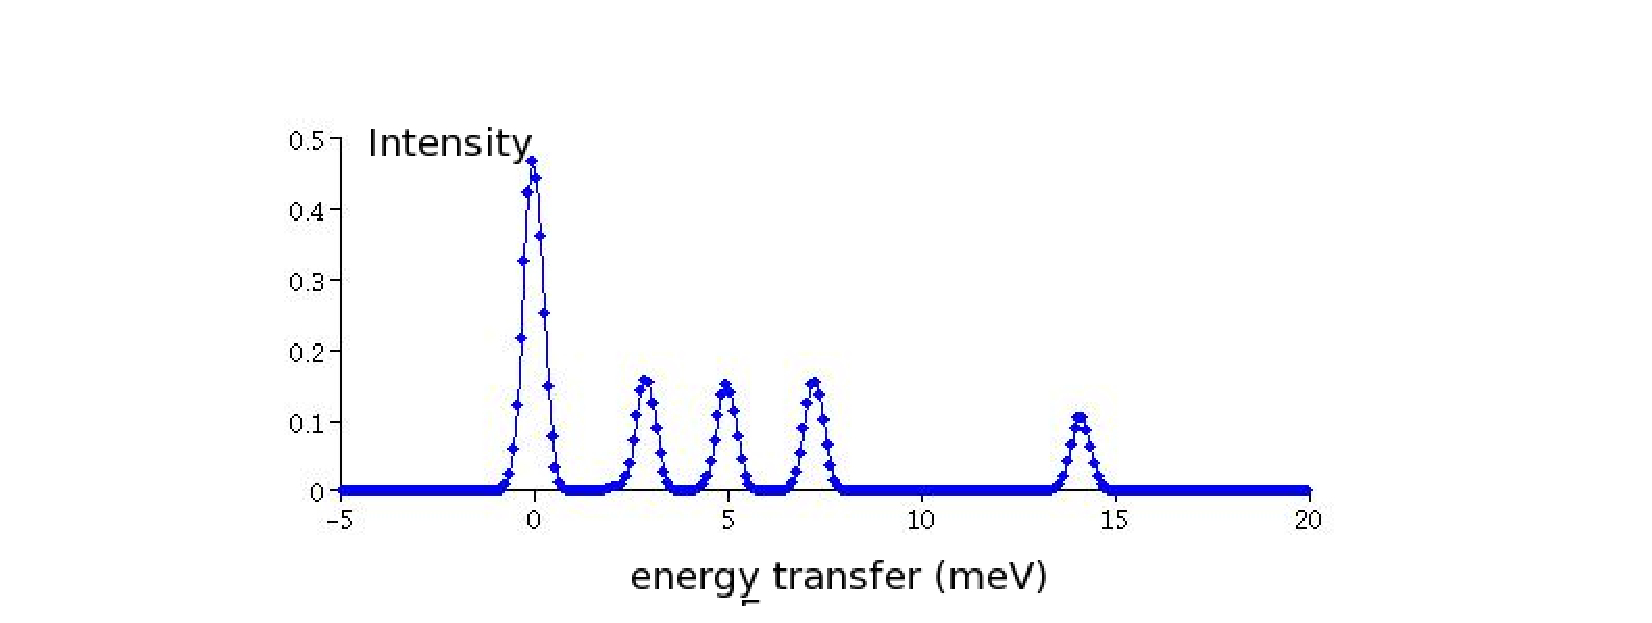
\includegraphics[angle=0,width=1.0\textwidth]{./figsrc/10KCEFspectrum.eps}
\caption{\label{spectrum}
Calculated crystal field neutron spectrum of NdCu$_2$ at a temperature of 10~K.
Horizontal axis is energy transfer in meV and vertical axis is neutron intensity
in barns per meV and Nd atom.
[plot created by program {\prg display}]}
\end{center}
\end{figure}
\item In order to calculate the magnetisation for our problem (in the paramagnetic state), the
direction of the magnetic field has to be given in {\prg bkq.parmeter} and
program {\prg so1ion\index{so1ion}} has to be started with the option {\prg -m}, i.e. {\bf so1ion -m -B 0 30 %%@
10}. The
numbers denote the field range (0-30 Tesla) and the temperature (10~K). The results are written
to {\prg moment.rtplot}, fig.~\ref{moment} shows the result.
\begin{figure}[ht]
\begin{center}
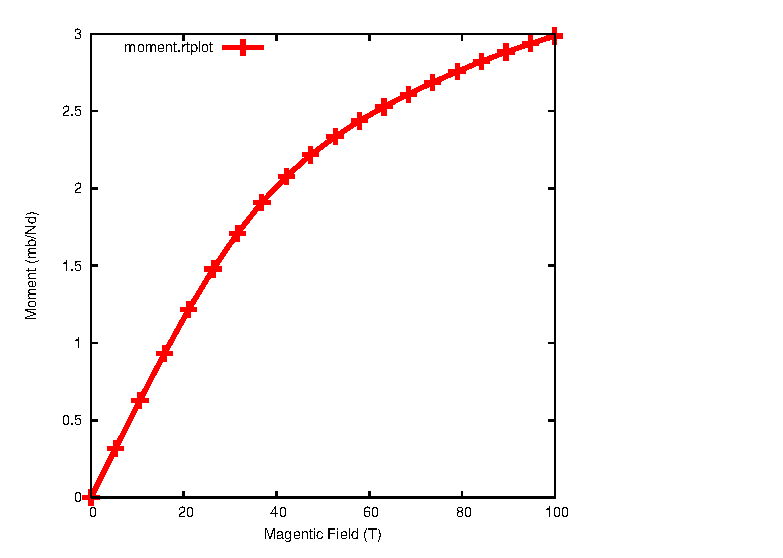
\includegraphics[angle=0,width=0.7\columnwidth]{./figsrc/moment.eps}
\caption{\label{moment}
Calculated magnetic moment for field applied along $x$ direction ($c$ axis, note the
notation of the crystal field $xyz$ axes with respect to the crystal lattice is
$xyz||cab$ in our example)
 of NdCu$_2$ at a temperature of 10~K.
[plot created by program {\prg gnuplot}]}
\end{center}
\end{figure}

\item In a similar way the temperature dependence of the susceptibility can be calculated by 
{\bf so1ion -s}. 
\item The crystal field contribution to the specific heat may be calculated 
from the output file {\prg so1ion.out} using the  program {\prg cpso1ion}, e.g. {\bf cpso1ion 10 100 1 %%@
[options]}
calculates the specific heat in the temperature interval 10-100 K with a step width
of 1 K. Alternatively a comparison to experimental data can be made by {\bf cpso1ion 1 2 cpexp.dat},
where the temperatures are given in column 1 and the experimental specific heat in column
2 of file cpexp.dat. The calculated specific heat is compared to the experimental data and
a standard deviation {\em sta} is calculated and output is written to stdout.
Other quantities can be calculated using the options: -s  (calculate entropy  (J/molK) instead of cp),
-f (calculate free energy (J/mol) instead of cp),-u  (calculate magnetic energy (J/mol) instead of cp),
-z (calculate partition sum instead of cp).
Fig.~\ref{cpndcu2} shows an example.
\begin{figure}[ht]
\begin{center}
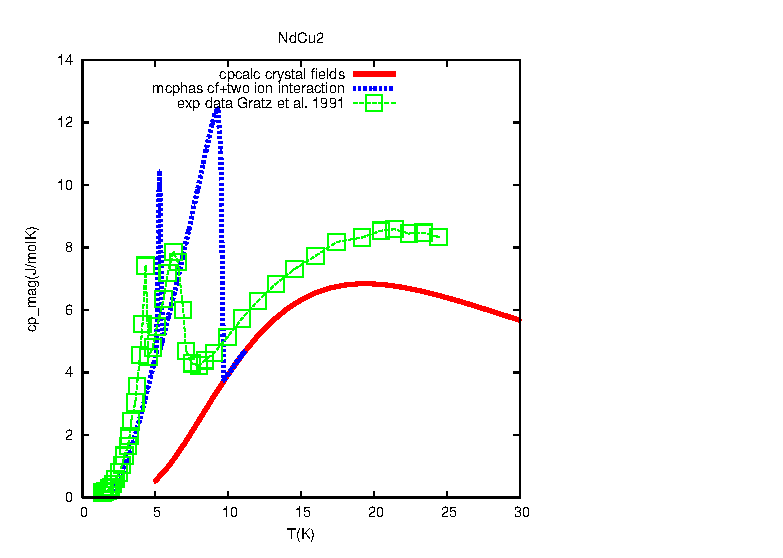
\includegraphics[angle=0,width=0.7\columnwidth]{./figsrc/cpall.eps}
\caption{\label{cpndcu2}
Calculated specific heat of NdCu$_2$ in zero magnetic field as calculated
by {\prg cpso1ion} (crystal field contribution) in comparison with experimental
data~\cite{gratz91-9297}. The dashed line shows the results of a calculation,
which in addition to the crystal field takes into account the two ion interaction
and using {\prg so1ion\index{so1ion}} as a module in {\prg mcphas} - see below and chapter~\ref{runmcphas}.
[plot created by program {\prg gnuplot}]}
\end{center}
\end{figure}
\end{enumerate}




\vspace{1cm}
{\em Exercises:}
\begin{itemize}
\item Use {\prg so1ion\index{so1ion}} to calculate the energies, eigenvectors and
transition matrix elements (for inelastic
neutron scattering) for Nd$^{3+}$ in an orthorhombic crystal field.
Use the parameters given in section~\ref{cf1ion}.
\end{itemize}



\subsection{Using {\prg so1ion\index{so1ion}} as a module in {\prg McPhase} and {\prg McDisp}}
\label{cf1ion}


The use 
 of {\prg so1ion\index{so1ion}} as a module in {\prg mcphas} is necessary in order to 
 go beyond the capabilities of {\prg so1ion\index{so1ion}} (for instance the calculation
 of magnetisation or specific heat or if the exchange interaction
 given in equations~(\ref{hamilton}) and (\ref{multipolehamilton})
  shall be taken into account).  

\subsubsection{Module Tasks:}


As a single ion module, {\prg so1ion\index{so1ion}} provides to {\prg mcphas} the magnetic properties
of a single rare earth ion subject to the crystal field. Its main duty is
to calculate the magnetic moment given an effective magnetic field. 
To be more explicit - given the effective magnetic field $H^s_{eff}$ by {\prg mcphas}
 the module {\prg so1ion\index{so1ion}}
 diagonalises the crystal field and Zeeman Hamiltonian (\ref{cfze}) of the
 ion $s$:

\begin{equation}\label{cfze}
 {\mathcal H}=  B_l^m O_{lm}({\mbf J}^s) 
	     -  g_{Ji} \mu_B {\mbf J}^s {\mbf H^s_{eff}} 
\end{equation}

and calculates the expectation value of the angular momentum $\langle \mbf J^s \rangle$
according to

\begin{equation}
\langle \mbf J^s \rangle =
\sum_{\Gamma} n_{\Gamma} \langle \Gamma | \mbf J^s | \Gamma \rangle
\end{equation}

with 

\begin{eqnarray}
n_{\Gamma}&=&\frac{\exp(-E_{\Gamma}/kT)}{z}\\
z&=&\sum_{\Gamma} \exp(-E_{\Gamma}/kT)
\end{eqnarray}

Here $z$ is the partition sum, $|\Gamma\rangle$ the eigenstate corresponding to
the eigenvalue $E_{\Gamma}$ of the Hamiltonian (\ref{cfze}). 
\footnote{In addition to $\langle \mbf J_i \rangle$ the module also returns
the partition sum $z$ and the magnetic energy $u=\sum_{\Gamma} n_{\Gamma} E_{\Gamma}$.}

\subsubsection{Module Usage:}
 

The program {\prg mcphas} (-calculation of the magnetic phase diagram) 
requires a single ion
property input file of the same format as given above in
section~\ref{cfieldexample} (also for each ion in the
crystallographic unit cell):

\begin{itemize}
\item The first line in the single ion property file tells {\prg mcphas} that the module
{\prg so1ion\index{so1ion}} should be used for this ion. 
\item Comment lines start with \#. 
\item The type of ion has to be given plus
several lines containing the crystal field parameters. 
\end{itemize}

It follows a simple  example (for more complicated examples see section \ref{sifile} and 
{\prg mcphas.cf1} in the 
directory {\prg examples/ndcu2b\_new}):


\begin{verbatim}
#!MODULE=so1ion
#<!--mcphas.cf-->
# comment followed by
# the ion type and the crystal field parameters [meV]
 IONTYPE=Nd3+
# - note you can also do any pure spin problem by entering e.g. IONTYPE=S=2.5 
 B20=  0.116765                                           
 B22  =  0.134172                                           
 B40  =  0.0019225                                          
 B42  =  0.0008704                                          
 B44  =  0.0016916                                          
 B60  =  0.0000476                                          
 B62  =  0.0000116                                          
 B64  =  0.0000421                                          
 B66  =  0.0003662                                          
\end{verbatim}


\begin{description}
\item [Note:] 
In order to use {\prg so1ion\index{so1ion}} as a module in {\prg McPhase} a convention for
the orientation of the $xyz$ coordinate system (of the crystal field) relative
to the crystal axis $abc$ has to be made:
 The axes convention adopted in module {\prg so1ion} for the crystal field parameters
is - $\mbf a||x$, $\mbf b||y$ and $\mbf c||z$. Note that if you use the
module {\prg cfield}, the choice is more unconventional:$\mbf a||y$, $\mbf b||z$ and $\mbf c||x$
Tools for rotating crystal field parameters are described in appendix~\ref{rotateBlm}.

The reason for
this unique choice is to make it possible to treat quadrupolar interactions - the 
generalisation of bilinear interactions to these higher order interactions
is much easier in this a first glance very unconventional axes convention.
Furthermore, for the higher order interactions it is also convenient to
adopt the same orientation of the coordinate system for each atom.


{\small
{\bf Information for experienced users:} the first line in the single ion property file
can either refer to  one of the standard
single ion property modules (e.g. Kramers ground state
doublet \#!MODULE=kramers, full crystal field \#!MODULE=so1ion) or a shared library file, which will be %%@
loaded
dynamically into the program at runtime 
 - for a description
of this file see section~\ref{sifile}.
}


\clearpage

\section{{\prg mcphas} - calculation of thermodynamic properties (Magnetisation, Susceptibility, Specific Heat, Neutron %%@
Diffraction, etc.)}
\label{runmcphas}

In order to perform calculations beyond the capabilities of {\prg cfield\index{cfield}} it is necessary
to use the program {\prg mcphas}. 
\begin{itemize}
\item As a first step it is possible to
calculate the thermodynamic properties such as magnetisation or specific heat
considering only single ion effects. In this case all the exchange parameters
have to be set to zero in {\prg mcphas.j\index{mcphas.j}}. 
\item for more advanced calculations the two - ion interactions have to be
considered and may lead to magnetic order. {\prg mcphas} can perform 
calculations in the ordered state in the following way: for 
a given temperature $T$ and magnetic field $\mbf H$ (vector)
several possible magnetic structures are stabilised
by a mean field algorithm and the free energy is 
calculated. The initial values for this mean-field procedure are
modified by a Monte Carlo process.


The temperature and magnetic field is varied during the calculation
and thereby it is possible to map out the magnetic phase diagram.
\end{itemize}

The program produces a plot of the stabilised magnetic
structures and the magnetisation on screen, the
output files contain additional information 
such as calculated magnetoelastic and  neutron-scattering
data. Several graphic programs easy the visualisation of the
calculated data (section~\ref{graphics}).



\subsection{Input Files}
The program {\prg McPhase} needs the following input files (all in the same directory)
 in order to run:

\begin{enumerate}
\item {\prg mcphas.ini\index{mcphas.ini}}
 - controlling the algorithm
\item {\prg mcphas.j\index{mcphas.j}}
  - lattice and exchange parameters
\item {\prg mcphas.tst\index{mcphas.tst}(optional)}  - test spin configurations
\item {\prg single-ion property files}
\item {\prg directory ./results/}
 - directory where calculated data is stored
\item {\prg directory ./fit} - experimental data for fit (optional)
\end{enumerate}


 All
 of these input files have to be in one directory and the program
has to be started in this directory. The results of the simulation
are then stored in the  subdirectory ./results/, which must exist before starting
the program 
... see directory ./examples/ for some examples.
 In order to prepare these files
for a new calculation it is best to take them from an example, copy the files
to a new directory and make the
modifications  to adapt them to the new problem.

\subsubsection{Example - a simple antiferromagnet}

In the following description of the input files we will always refer
to a simple example: a simple antiferromagnet
on a primitive orthorhombic lattice. The first time user
will thus have a simple example to follow, all corresponding
files are given in the directory {\prg tutorial/03magnetic\_phases\_mcphas/simpleAF}.
 

\subsubsection{{\prg mcphas.ini\index{mcphas.ini}} - controlling the algorithm}
   Initial file containing algorithm control parameters, for instance the range and spacing of
   propagation vectors Q or the number of Monte Carlo trials for initial spin configurations
    - {\em mind}: this
   file is rewritten and reread  when running the program and may be changed by the
   user in order to manipulate the running simulation.

{\prg mcphas.ini\index{mcphas.ini}} consists of several sections:
\begin{description}
\item [MCPHASE RUNTIME CONTROL:] this section contains the parameters
controlling the status of the calculation.
\item [XY PHASEDIAGRAM PARAMETERS:] here the temperature and field range and
step widths of the calculation are specified.
The definition of the x and y
axis in terms of temperature and magnetic field is followed by the
corresponding range and step width. An offset may be given for all
field and temperature values.
Note that for most cases of interest
this offset is zero (T0=0, Ha0=0, Hb0=0, Hc0=0).
 For the simple case of calculating a Temperature-Field phase diagram
 It is just necessary to set xT=1 and give the temperature range by
xmin/xmax/xstep. For field in b direction then just set yHb=1 and 
define the range in ymin/ymax/ystep.
In case of non-orthogonal axes the applied magnetic field
components $Ha, Hb, Hc$ refer to the orthogonal coordinate system
defined with respect to the nonorthogonal lattice $\mbf a,\mbf b,\mbf c$ as
$Hb||\mbf b$, $Hc||(\mbf a \times \mbf b)$ and $Ha$ perpendicular to $Hb$ and $Hc$.

\item [GENERATION OF SPINCONFIGURATIONS:] at the beginning of the program
some initial values of spin configurations are generated from a set of 
propagation vectors. This section defines the range of propagation vectors
and the step width.
Depending on the value of the propagation Q with respect to the primitive reciprocal lattice
1-, 2- or 3-dimensional simulations of magnetic lattices
are possible. It is advisable to 
think carefully about the chosen range and spacing of Q vectors in order
to limit calculation time.
 
For example a good starting point is to begin with a calculation with large
step widths (e.g. 0.1)  covering the Brillouin zone. This should give an idea
of the propagation vectors which are stabilised. An advanced calculation
could then fine tune the propagation and determine its accurate value (using
small step widths in a limited area of the zone).
The verbose option of {\prg mcphas} allows to inspect the propagation vectors
which are actually used in the calculation.
Trick: in order to get a quick overview of the
q-vector range covered by the mcphas\index{mcphas} simulation start mcphas, exit and 
just type {\prg felog ./results/mcphas.qvc} (need {\prg perl,perldl,pdl,pgplot} packages).

In order to limit calculation time, the maximum periodicity
of the magnetic unit cell with respect to the crystallographic unit cell 
(maxqperiod) and the maximum number of spins in the magnetic unit cell 
(maxnofspins) can be limited. Also the maximum number of test spin configurations
in the internal table can be limited (maxnoftestspincf).
A critical feature with respect to calculation time is also the number of
spin configurations which are generated by a random process from a tabulated
SPINCONFIGURATIONS during the calculation. 

In summary the variables in this section are mainly important to adapt the
program to a given computer system with finite speed. They have to be set
to optimise between speed and accuracy of the calculation. In order to
find appropriate values it is best to perform some calculations 
and restrict the parameters step by step if insufficient speed is obtained.
Also the examples included in the program package may serve as starting
points.

\item [PARAMETERS FOR SUB FECALC SELFCONSISTENCY PROCESS:] the most important
procedure in the module {\prg mcphas} is the sub fecalc. In this part of the 
program the self consistent calculation of the magnetic moment configuration
is performed as shown schematically in fig.~\ref{fecalc}. 
In the mean field approximation the Hamiltonian~(\ref{hamilton}) is approximated
by

\begin{equation}
 {\mathcal H}=\sum_n H_{SI}^n + E_{corr}
\end{equation}

with the single ion Hamiltonian (in case of module {\prg so1ion\index{so1ion}})

\begin{equation}
H_{SI}^n=  B_l^m O_{lm}({\mbf J}^n) 
	     - g_{Jn} \mu_B {\mbf J}^n {\mbf H^n_{eff}} 
\end{equation}

and the correction term

\begin{equation}
E_{corr}=\frac{1}{2}\sum_{n} g_{Jn} \mu_B \langle {\mbf J}^n
 \rangle (\mbf H^n_{eff}-\mbf H) 
\end{equation}

and with the mean fields $ \mbf H^n_{eff}$ given by

\begin{equation}\label{meanfield}
\mbf H^n_{eff}=\mbf H + \mbf H^n_{xc}=\mbf H+\sum_{{\mbf G'}n'} \frac{{\mathcal J}
(\mbf r_n-(\mbf G'+\mbf r_{n'}))}{g_{Jn}\mu_B } \langle{\mbf
J}^{n'}\rangle
\end{equation}

These mean fields and the moments $\langle \mbf J^n \rangle$ 
are determined in a self consistent
way. For a given magnetic unit cell and initial configuration 
of magnetic moments
the mean fields are calculated according to equation~(\ref{meanfield}). 
Then, for each
magnetic ion the single ion property module is taken 
and the magnetic moment $\langle \mbf J^n \rangle$ is 
calculated from it's mean field. The mean fields are used again in equation~(\ref{meanfield})
and so on .... until convergence is reached. 
Then, the free energy ($f=-kT\sum_n \ln(z_n) + E_{corr}$ ) 
of the stabilised
configuration is calculated (this is why this sub is called {\prg fecalc}). 
The free energies of a lot of different stabilised configurations have to
be compared in order to find out which configuration has lowest free energy, i.e.
is stable in thermal  equilibrium.

It may happen that this process does
not converge due to bad choice of the initial configuration, therefore a maximum number
of mean field loops has to be given by the user.
The results of a calculation may be significantly influenced by
changing parameters such as the maximum number of iteration loops 
in this section. 
In fact the simulation is always a compromise of calculation time and accuracy: if only
a few initial spin configurations are tried at each (H-T) point, the calculation speed is
fast, however it is possible that the program misses the magnetic structure with the
lowest free energy. The same holds if other critical parameters of the simulation are
restricted too much.
 

\item [OUTPUT OF PHYSICAL PROPERTIES:]
Some options for the output of the calculation can be changed in this section.
\end{description}

\begin{figure}[hb]
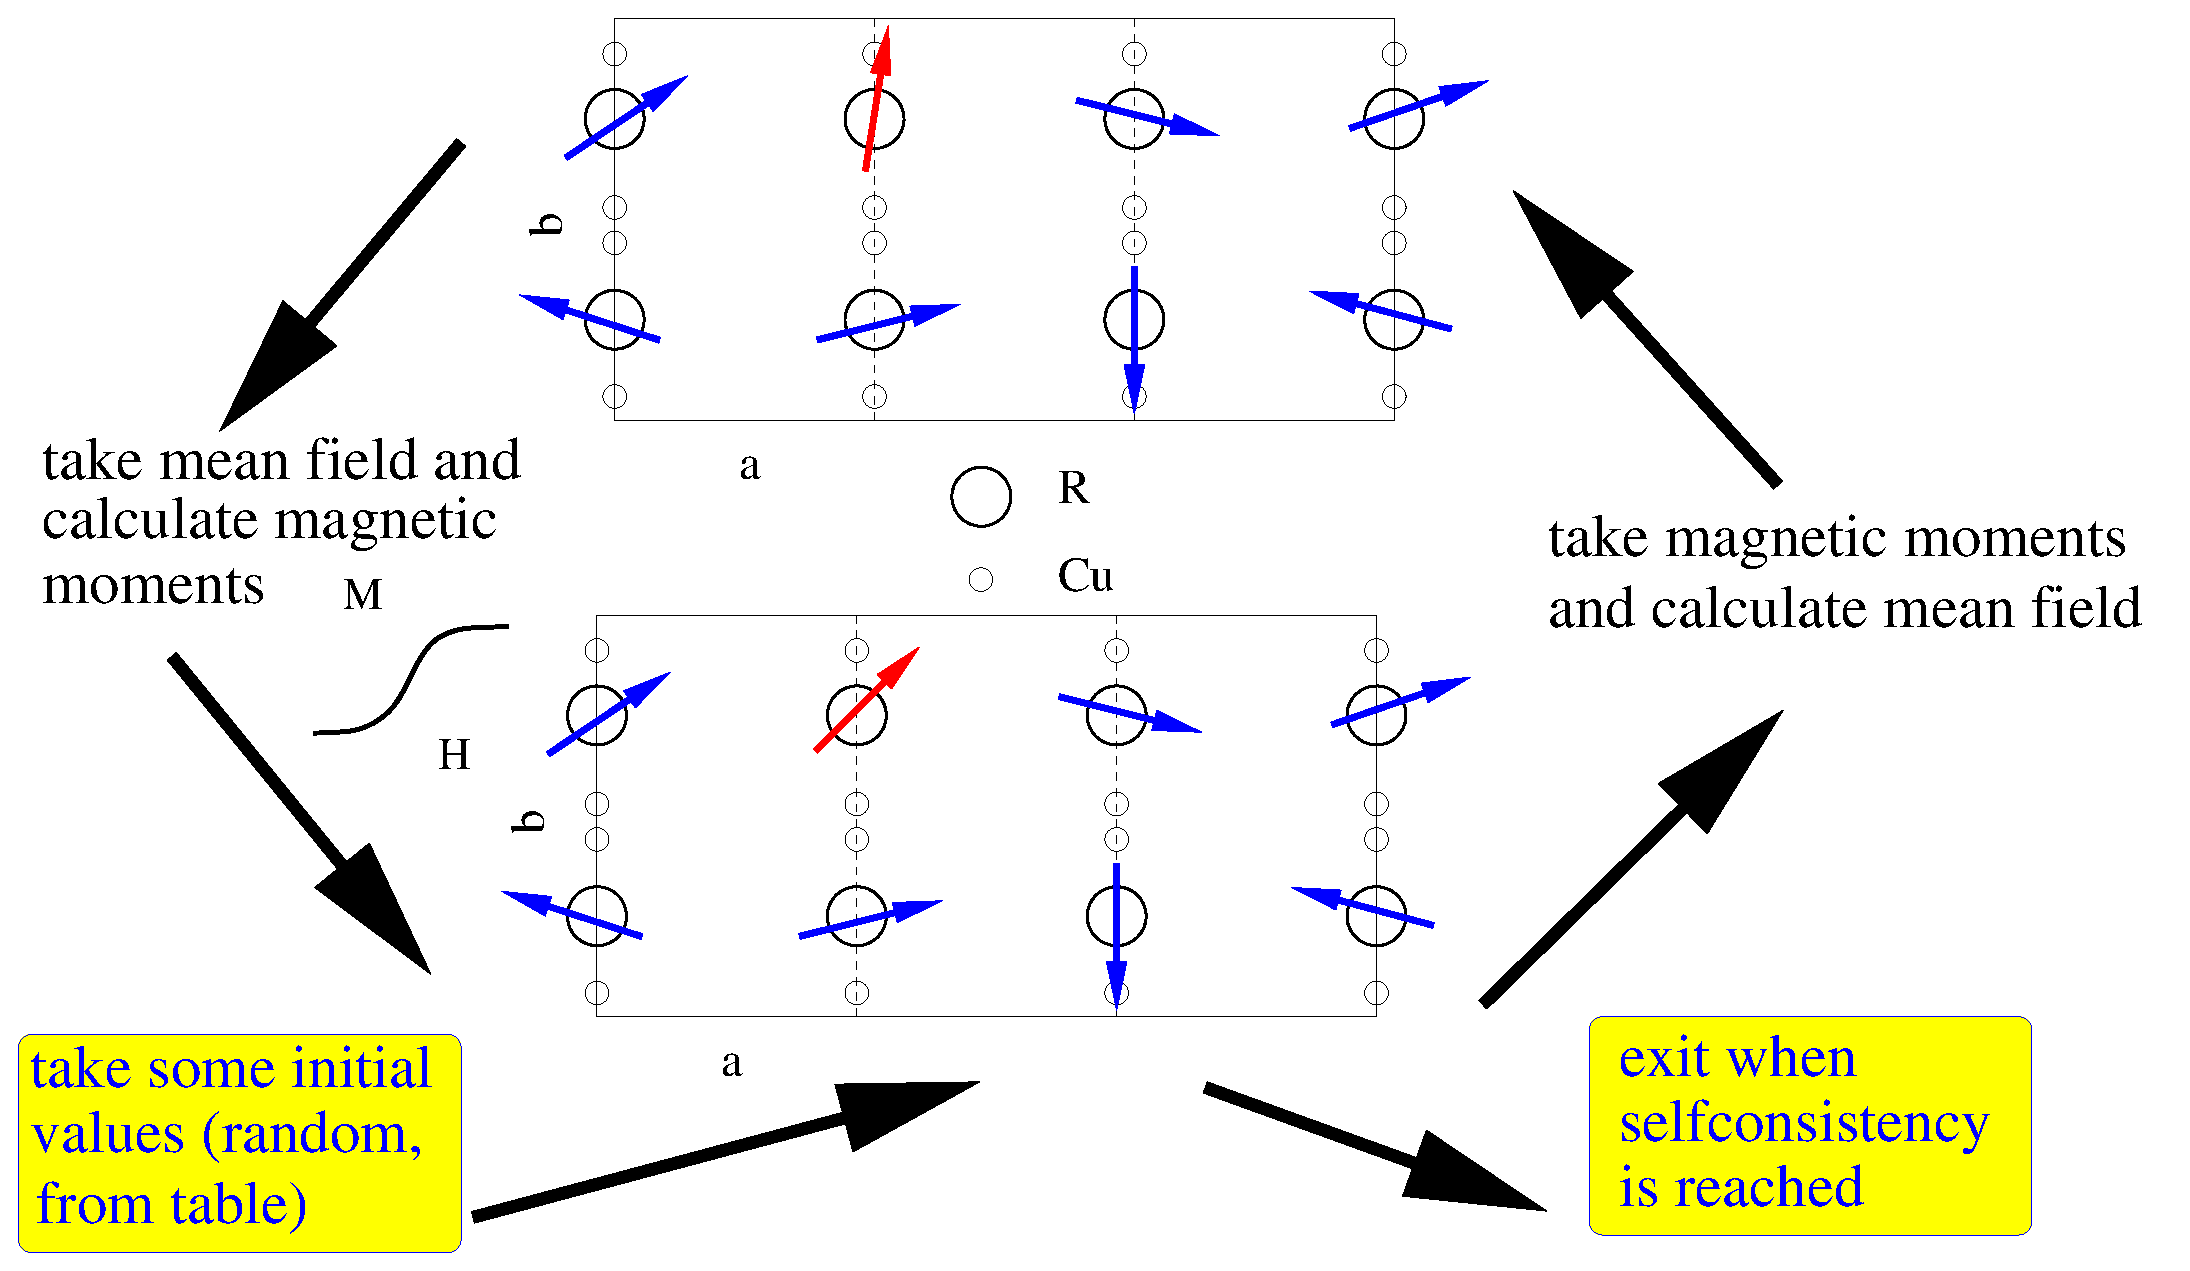
\includegraphics[angle=0,width=0.9\columnwidth]{figsrc/fecalc.eps}
\caption{\label{fecalc}Mean field process of sub {\prg fecalc}.}
\end{figure}

 
\subsubsection{Example {\prg mcphas.ini\index{mcphas.ini}} file for a simple antiferromagnet}

Here is an example of {\prg mcphas.ini\index{mcphas.ini}}, the comments describe the meaning of the different
parameters:

\section{{\prg mcphas} - calculation of thermodynamic properties (Magnetisation, Susceptibility, Specific Heat, Neutron %%@
Diffraction, etc.)}
\label{runmcphas}

In order to perform calculations beyond the capabilities of {\prg cfield\index{cfield}} it is necessary
to use the program {\prg mcphas}. 
\begin{itemize}
\item As a first step it is possible to
calculate the thermodynamic properties such as magnetisation or specific heat
considering only single ion effects. In this case all the exchange parameters
have to be set to zero in {\prg mcphas.j\index{mcphas.j}}. 
\item for more advanced calculations the two - ion interactions have to be
considered and may lead to magnetic order. {\prg mcphas} can perform 
calculations in the ordered state in the following way: for 
a given temperature $T$ and magnetic field $\mbf H$ (vector)
several possible magnetic structures are stabilised
by a mean field algorithm and the free energy is 
calculated. The initial values for this mean-field procedure are
modified by a Monte Carlo process.


The temperature and magnetic field is varied during the calculation
and thereby it is possible to map out the magnetic phase diagram.
\end{itemize}

The program produces a plot of the stabilised magnetic
structures and the magnetisation on screen, the
output files contain additional information 
such as calculated magnetoelastic and  neutron-scattering
data. Several graphic programs easy the visualisation of the
calculated data (section~\ref{graphics}).



\subsection{Input Files}
The program {\prg McPhase} needs the following input files (all in the same directory)
 in order to run:

\begin{enumerate}
\item {\prg mcphas.ini\index{mcphas.ini}}
 - controlling the algorithm
\item {\prg mcphas.j\index{mcphas.j}}
  - lattice and exchange parameters
\item {\prg mcphas.tst\index{mcphas.tst}(optional)}  - test spin configurations
\item {\prg single-ion property files}
\item {\prg directory ./results/}
 - directory where calculated data is stored
\item {\prg directory ./fit} - experimental data for fit (optional)
\end{enumerate}


 All
 of these input files have to be in one directory and the program
has to be started in this directory. The results of the simulation
are then stored in the  subdirectory ./results/, which must exist before starting
the program 
... see directory ./examples/ for some examples.
 In order to prepare these files
for a new calculation it is best to take them from an example, copy the files
to a new directory and make the
modifications  to adapt them to the new problem.

\subsubsection{Example - a simple antiferromagnet}

In the following description of the input files we will always refer
to a simple example: a simple antiferromagnet
on a primitive orthorhombic lattice. The first time user
will thus have a simple example to follow, all corresponding
files are given in the directory {\prg tutorial/03magnetic\_phases\_mcphas/simpleAF}.
 

\subsubsection{{\prg mcphas.ini\index{mcphas.ini}} - controlling the algorithm}
   Initial file containing algorithm control parameters, for instance the range and spacing of
   propagation vectors Q or the number of Monte Carlo trials for initial spin configurations
    - {\em mind}: this
   file is rewritten and reread  when running the program and may be changed by the
   user in order to manipulate the running simulation.

{\prg mcphas.ini\index{mcphas.ini}} consists of several sections:
\begin{description}
\item [MCPHASE RUNTIME CONTROL:] this section contains the parameters
controlling the status of the calculation.
\item [XY PHASEDIAGRAM PARAMETERS:] here the temperature and field range and
step widths of the calculation are specified.
The definition of the x and y
axis in terms of temperature and magnetic field is followed by the
corresponding range and step width. An offset may be given for all
field and temperature values.
Note that for most cases of interest
this offset is zero (T0=0, Ha0=0, Hb0=0, Hc0=0).
 For the simple case of calculating a Temperature-Field phase diagram
 It is just necessary to set xT=1 and give the temperature range by
xmin/xmax/xstep. For field in b direction then just set yHb=1 and 
define the range in ymin/ymax/ystep.
In case of non-orthogonal axes the applied magnetic field
components $Ha, Hb, Hc$ refer to the orthogonal coordinate system
defined with respect to the nonorthogonal lattice $\mbf a,\mbf b,\mbf c$ as
$Hb||\mbf b$, $Hc||(\mbf a \times \mbf b)$ and $Ha$ perpendicular to $Hb$ and $Hc$.

\item [GENERATION OF SPINCONFIGURATIONS:] at the beginning of the program
some initial values of spin configurations are generated from a set of 
propagation vectors. This section defines the range of propagation vectors
and the step width.
Depending on the value of the propagation Q with respect to the primitive reciprocal lattice
1-, 2- or 3-dimensional simulations of magnetic lattices
are possible. It is advisable to 
think carefully about the chosen range and spacing of Q vectors in order
to limit calculation time.
 
For example a good starting point is to begin with a calculation with large
step widths (e.g. 0.1)  covering the Brillouin zone. This should give an idea
of the propagation vectors which are stabilised. An advanced calculation
could then fine tune the propagation and determine its accurate value (using
small step widths in a limited area of the zone).
The verbose option of {\prg mcphas} allows to inspect the propagation vectors
which are actually used in the calculation.
Trick: in order to get a quick overview of the
q-vector range covered by the mcphas\index{mcphas} simulation start mcphas, exit and 
just type {\prg felog ./results/mcphas.qvc} (need {\prg perl,perldl,pdl,pgplot} packages).

In order to limit calculation time, the maximum periodicity
of the magnetic unit cell with respect to the crystallographic unit cell 
(maxqperiod) and the maximum number of spins in the magnetic unit cell 
(maxnofspins) can be limited. Also the maximum number of test spin configurations
in the internal table can be limited (maxnoftestspincf).
A critical feature with respect to calculation time is also the number of
spin configurations which are generated by a random process from a tabulated
SPINCONFIGURATIONS during the calculation. 

In summary the variables in this section are mainly important to adapt the
program to a given computer system with finite speed. They have to be set
to optimise between speed and accuracy of the calculation. In order to
find appropriate values it is best to perform some calculations 
and restrict the parameters step by step if insufficient speed is obtained.
Also the examples included in the program package may serve as starting
points.

\item [PARAMETERS FOR SUB FECALC SELFCONSISTENCY PROCESS:] the most important
procedure in the module {\prg mcphas} is the sub fecalc. In this part of the 
program the self consistent calculation of the magnetic moment configuration
is performed as shown schematically in fig.~\ref{fecalc}. 
In the mean field approximation the Hamiltonian~(\ref{hamilton}) is approximated
by

\begin{equation}
 {\mathcal H}=\sum_n H_{SI}^n + E_{corr}
\end{equation}

with the single ion Hamiltonian (in case of module {\prg so1ion\index{so1ion}})

\begin{equation}
H_{SI}^n=  B_l^m O_{lm}({\mbf J}^n) 
	     - g_{Jn} \mu_B {\mbf J}^n {\mbf H^n_{eff}} 
\end{equation}

and the correction term

\begin{equation}
E_{corr}=\frac{1}{2}\sum_{n} g_{Jn} \mu_B \langle {\mbf J}^n
 \rangle (\mbf H^n_{eff}-\mbf H) 
\end{equation}

and with the mean fields $ \mbf H^n_{eff}$ given by

\begin{equation}\label{meanfield}
\mbf H^n_{eff}=\mbf H + \mbf H^n_{xc}=\mbf H+\sum_{{\mbf G'}n'} \frac{{\mathcal J}
(\mbf r_n-(\mbf G'+\mbf r_{n'}))}{g_{Jn}\mu_B } \langle{\mbf
J}^{n'}\rangle
\end{equation}

These mean fields and the moments $\langle \mbf J^n \rangle$ 
are determined in a self consistent
way. For a given magnetic unit cell and initial configuration 
of magnetic moments
the mean fields are calculated according to equation~(\ref{meanfield}). 
Then, for each
magnetic ion the single ion property module is taken 
and the magnetic moment $\langle \mbf J^n \rangle$ is 
calculated from it's mean field. The mean fields are used again in equation~(\ref{meanfield})
and so on .... until convergence is reached. 
Then, the free energy ($f=-kT\sum_n \ln(z_n) + E_{corr}$ ) 
of the stabilised
configuration is calculated (this is why this sub is called {\prg fecalc}). 
The free energies of a lot of different stabilised configurations have to
be compared in order to find out which configuration has lowest free energy, i.e.
is stable in thermal  equilibrium.

It may happen that this process does
not converge due to bad choice of the initial configuration, therefore a maximum number
of mean field loops has to be given by the user.
The results of a calculation may be significantly influenced by
changing parameters such as the maximum number of iteration loops 
in this section. 
In fact the simulation is always a compromise of calculation time and accuracy: if only
a few initial spin configurations are tried at each (H-T) point, the calculation speed is
fast, however it is possible that the program misses the magnetic structure with the
lowest free energy. The same holds if other critical parameters of the simulation are
restricted too much.
 

\item [OUTPUT OF PHYSICAL PROPERTIES:]
Some options for the output of the calculation can be changed in this section.
\end{description}

\begin{figure}[hb]
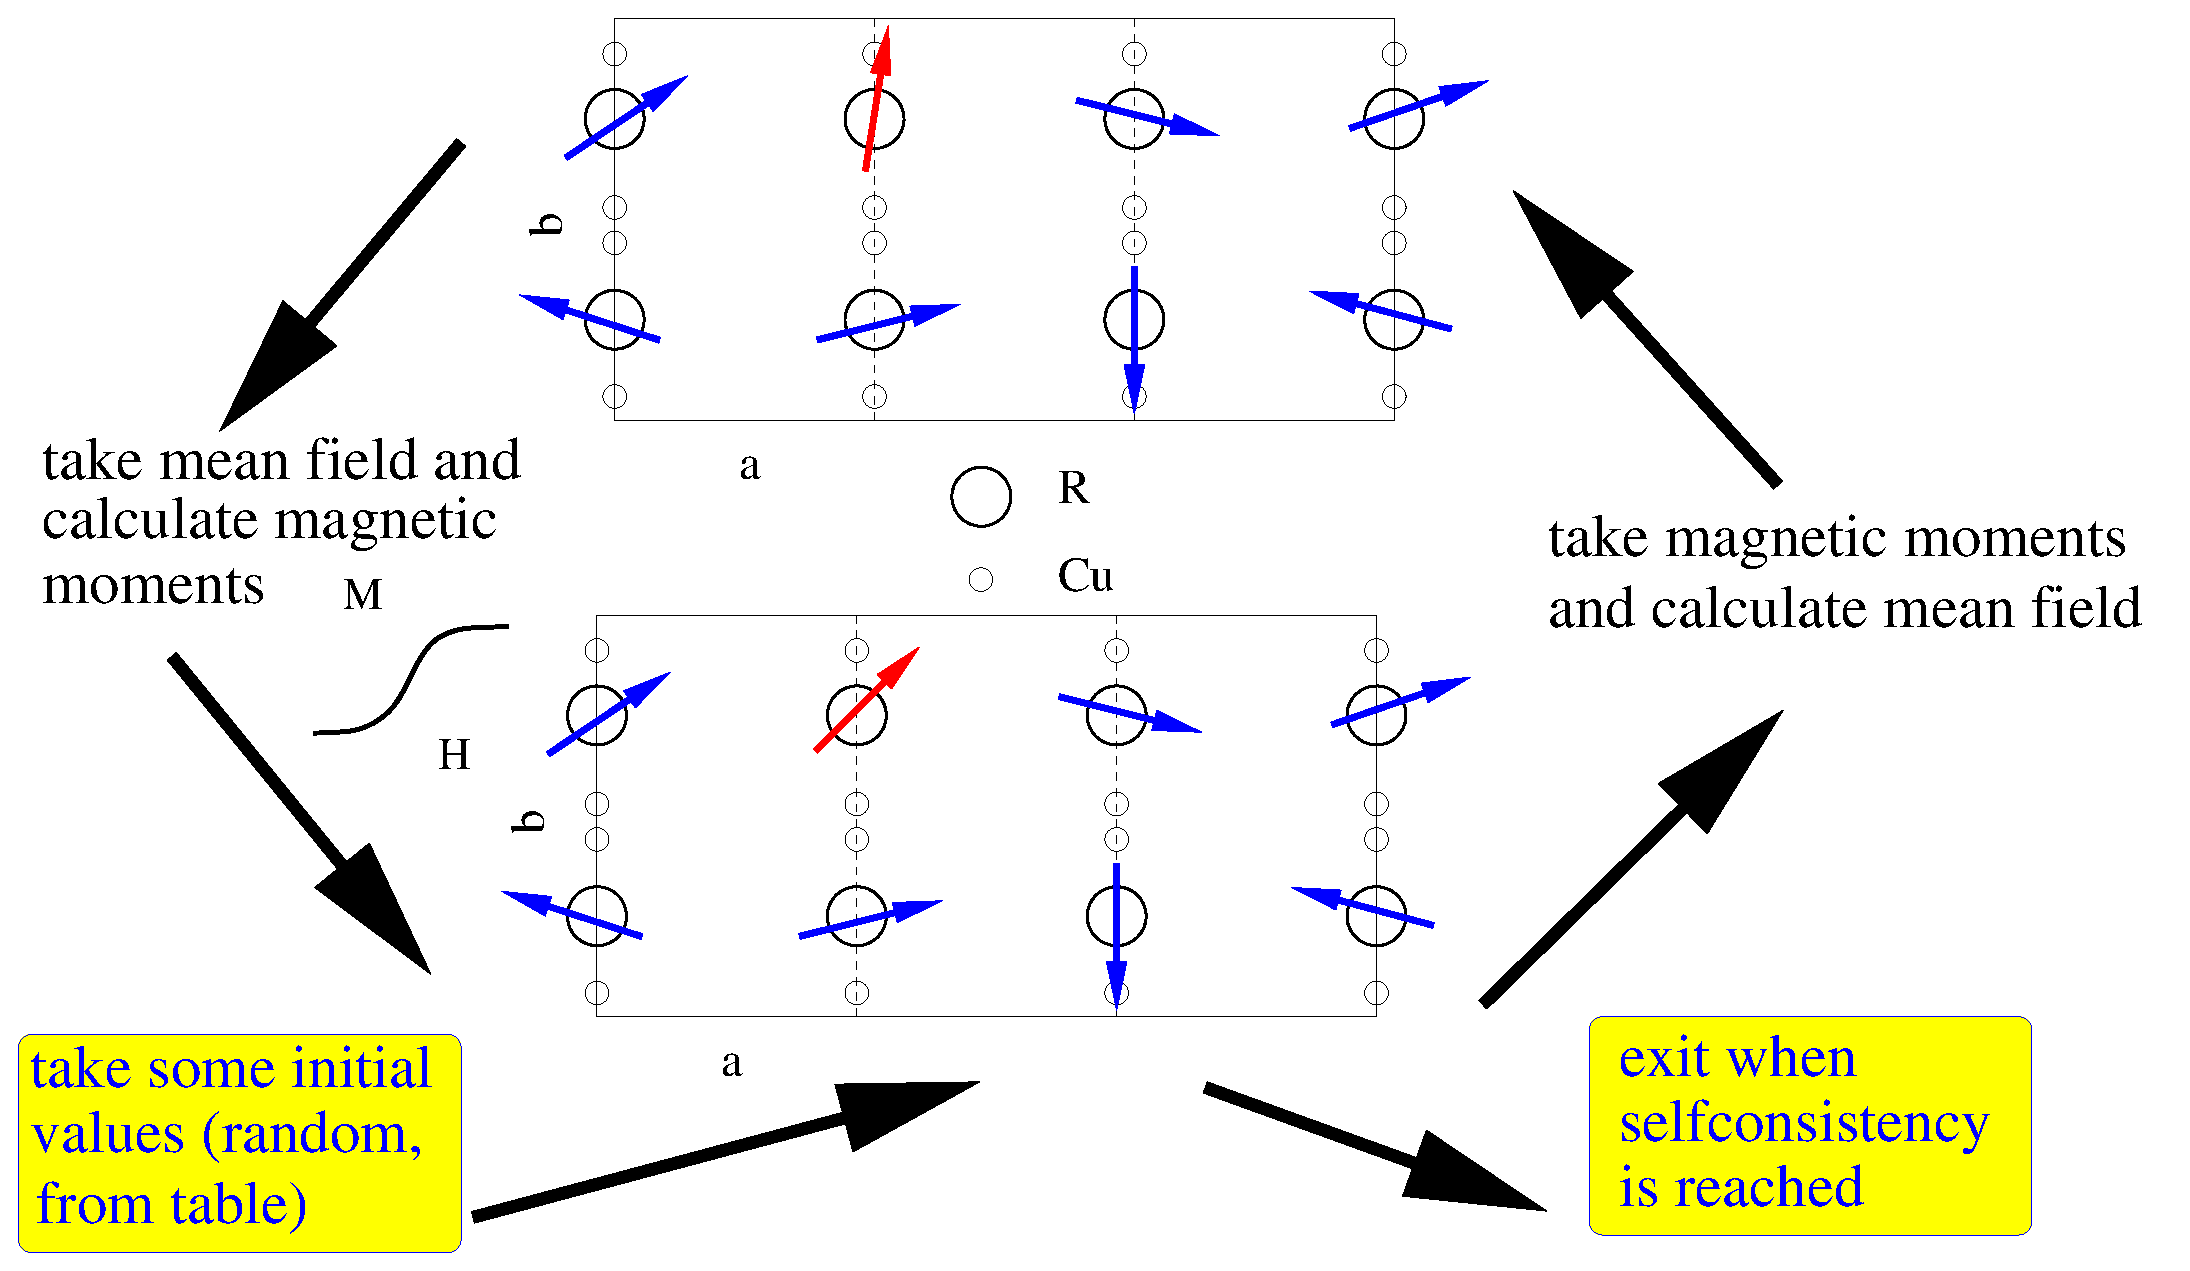
\includegraphics[angle=0,width=0.9\columnwidth]{figsrc/fecalc.eps}
\caption{\label{fecalc}Mean field process of sub {\prg fecalc}.}
\end{figure}

 
\subsubsection{Example {\prg mcphas.ini\index{mcphas.ini}} file for a simple antiferromagnet}

Here is an example of {\prg mcphas.ini\index{mcphas.ini}}, the comments describe the meaning of the different
parameters:

\section{{\prg mcphas} - calculation of thermodynamic properties (Magnetisation, Susceptibility, Specific Heat, Neutron %%@
Diffraction, etc.)}
\label{runmcphas}

In order to perform calculations beyond the capabilities of {\prg cfield\index{cfield}} it is necessary
to use the program {\prg mcphas}. 
\begin{itemize}
\item As a first step it is possible to
calculate the thermodynamic properties such as magnetisation or specific heat
considering only single ion effects. In this case all the exchange parameters
have to be set to zero in {\prg mcphas.j\index{mcphas.j}}. 
\item for more advanced calculations the two - ion interactions have to be
considered and may lead to magnetic order. {\prg mcphas} can perform 
calculations in the ordered state in the following way: for 
a given temperature $T$ and magnetic field $\mbf H$ (vector)
several possible magnetic structures are stabilised
by a mean field algorithm and the free energy is 
calculated. The initial values for this mean-field procedure are
modified by a Monte Carlo process.


The temperature and magnetic field is varied during the calculation
and thereby it is possible to map out the magnetic phase diagram.
\end{itemize}

The program produces a plot of the stabilised magnetic
structures and the magnetisation on screen, the
output files contain additional information 
such as calculated magnetoelastic and  neutron-scattering
data. Several graphic programs easy the visualisation of the
calculated data (section~\ref{graphics}).



\subsection{Input Files}
The program {\prg McPhase} needs the following input files (all in the same directory)
 in order to run:

\begin{enumerate}
\item {\prg mcphas.ini\index{mcphas.ini}}
 - controlling the algorithm
\item {\prg mcphas.j\index{mcphas.j}}
  - lattice and exchange parameters
\item {\prg mcphas.tst\index{mcphas.tst}(optional)}  - test spin configurations
\item {\prg single-ion property files}
\item {\prg directory ./results/}
 - directory where calculated data is stored
\item {\prg directory ./fit} - experimental data for fit (optional)
\end{enumerate}


 All
 of these input files have to be in one directory and the program
has to be started in this directory. The results of the simulation
are then stored in the  subdirectory ./results/, which must exist before starting
the program 
... see directory ./examples/ for some examples.
 In order to prepare these files
for a new calculation it is best to take them from an example, copy the files
to a new directory and make the
modifications  to adapt them to the new problem.

\subsubsection{Example - a simple antiferromagnet}

In the following description of the input files we will always refer
to a simple example: a simple antiferromagnet
on a primitive orthorhombic lattice. The first time user
will thus have a simple example to follow, all corresponding
files are given in the directory {\prg tutorial/03magnetic\_phases\_mcphas/simpleAF}.
 

\subsubsection{{\prg mcphas.ini\index{mcphas.ini}} - controlling the algorithm}
   Initial file containing algorithm control parameters, for instance the range and spacing of
   propagation vectors Q or the number of Monte Carlo trials for initial spin configurations
    - {\em mind}: this
   file is rewritten and reread  when running the program and may be changed by the
   user in order to manipulate the running simulation.

{\prg mcphas.ini\index{mcphas.ini}} consists of several sections:
\begin{description}
\item [MCPHASE RUNTIME CONTROL:] this section contains the parameters
controlling the status of the calculation.
\item [XY PHASEDIAGRAM PARAMETERS:] here the temperature and field range and
step widths of the calculation are specified.
The definition of the x and y
axis in terms of temperature and magnetic field is followed by the
corresponding range and step width. An offset may be given for all
field and temperature values.
Note that for most cases of interest
this offset is zero (T0=0, Ha0=0, Hb0=0, Hc0=0).
 For the simple case of calculating a Temperature-Field phase diagram
 It is just necessary to set xT=1 and give the temperature range by
xmin/xmax/xstep. For field in b direction then just set yHb=1 and 
define the range in ymin/ymax/ystep.
In case of non-orthogonal axes the applied magnetic field
components $Ha, Hb, Hc$ refer to the orthogonal coordinate system
defined with respect to the nonorthogonal lattice $\mbf a,\mbf b,\mbf c$ as
$Hb||\mbf b$, $Hc||(\mbf a \times \mbf b)$ and $Ha$ perpendicular to $Hb$ and $Hc$.

\item [GENERATION OF SPINCONFIGURATIONS:] at the beginning of the program
some initial values of spin configurations are generated from a set of 
propagation vectors. This section defines the range of propagation vectors
and the step width.
Depending on the value of the propagation Q with respect to the primitive reciprocal lattice
1-, 2- or 3-dimensional simulations of magnetic lattices
are possible. It is advisable to 
think carefully about the chosen range and spacing of Q vectors in order
to limit calculation time.
 
For example a good starting point is to begin with a calculation with large
step widths (e.g. 0.1)  covering the Brillouin zone. This should give an idea
of the propagation vectors which are stabilised. An advanced calculation
could then fine tune the propagation and determine its accurate value (using
small step widths in a limited area of the zone).
The verbose option of {\prg mcphas} allows to inspect the propagation vectors
which are actually used in the calculation.
Trick: in order to get a quick overview of the
q-vector range covered by the mcphas\index{mcphas} simulation start mcphas, exit and 
just type {\prg felog ./results/mcphas.qvc} (need {\prg perl,perldl,pdl,pgplot} packages).

In order to limit calculation time, the maximum periodicity
of the magnetic unit cell with respect to the crystallographic unit cell 
(maxqperiod) and the maximum number of spins in the magnetic unit cell 
(maxnofspins) can be limited. Also the maximum number of test spin configurations
in the internal table can be limited (maxnoftestspincf).
A critical feature with respect to calculation time is also the number of
spin configurations which are generated by a random process from a tabulated
SPINCONFIGURATIONS during the calculation. 

In summary the variables in this section are mainly important to adapt the
program to a given computer system with finite speed. They have to be set
to optimise between speed and accuracy of the calculation. In order to
find appropriate values it is best to perform some calculations 
and restrict the parameters step by step if insufficient speed is obtained.
Also the examples included in the program package may serve as starting
points.

\item [PARAMETERS FOR SUB FECALC SELFCONSISTENCY PROCESS:] the most important
procedure in the module {\prg mcphas} is the sub fecalc. In this part of the 
program the self consistent calculation of the magnetic moment configuration
is performed as shown schematically in fig.~\ref{fecalc}. 
In the mean field approximation the Hamiltonian~(\ref{hamilton}) is approximated
by

\begin{equation}
 {\mathcal H}=\sum_n H_{SI}^n + E_{corr}
\end{equation}

with the single ion Hamiltonian (in case of module {\prg so1ion\index{so1ion}})

\begin{equation}
H_{SI}^n=  B_l^m O_{lm}({\mbf J}^n) 
	     - g_{Jn} \mu_B {\mbf J}^n {\mbf H^n_{eff}} 
\end{equation}

and the correction term

\begin{equation}
E_{corr}=\frac{1}{2}\sum_{n} g_{Jn} \mu_B \langle {\mbf J}^n
 \rangle (\mbf H^n_{eff}-\mbf H) 
\end{equation}

and with the mean fields $ \mbf H^n_{eff}$ given by

\begin{equation}\label{meanfield}
\mbf H^n_{eff}=\mbf H + \mbf H^n_{xc}=\mbf H+\sum_{{\mbf G'}n'} \frac{{\mathcal J}
(\mbf r_n-(\mbf G'+\mbf r_{n'}))}{g_{Jn}\mu_B } \langle{\mbf
J}^{n'}\rangle
\end{equation}

These mean fields and the moments $\langle \mbf J^n \rangle$ 
are determined in a self consistent
way. For a given magnetic unit cell and initial configuration 
of magnetic moments
the mean fields are calculated according to equation~(\ref{meanfield}). 
Then, for each
magnetic ion the single ion property module is taken 
and the magnetic moment $\langle \mbf J^n \rangle$ is 
calculated from it's mean field. The mean fields are used again in equation~(\ref{meanfield})
and so on .... until convergence is reached. 
Then, the free energy ($f=-kT\sum_n \ln(z_n) + E_{corr}$ ) 
of the stabilised
configuration is calculated (this is why this sub is called {\prg fecalc}). 
The free energies of a lot of different stabilised configurations have to
be compared in order to find out which configuration has lowest free energy, i.e.
is stable in thermal  equilibrium.

It may happen that this process does
not converge due to bad choice of the initial configuration, therefore a maximum number
of mean field loops has to be given by the user.
The results of a calculation may be significantly influenced by
changing parameters such as the maximum number of iteration loops 
in this section. 
In fact the simulation is always a compromise of calculation time and accuracy: if only
a few initial spin configurations are tried at each (H-T) point, the calculation speed is
fast, however it is possible that the program misses the magnetic structure with the
lowest free energy. The same holds if other critical parameters of the simulation are
restricted too much.
 

\item [OUTPUT OF PHYSICAL PROPERTIES:]
Some options for the output of the calculation can be changed in this section.
\end{description}

\begin{figure}[hb]
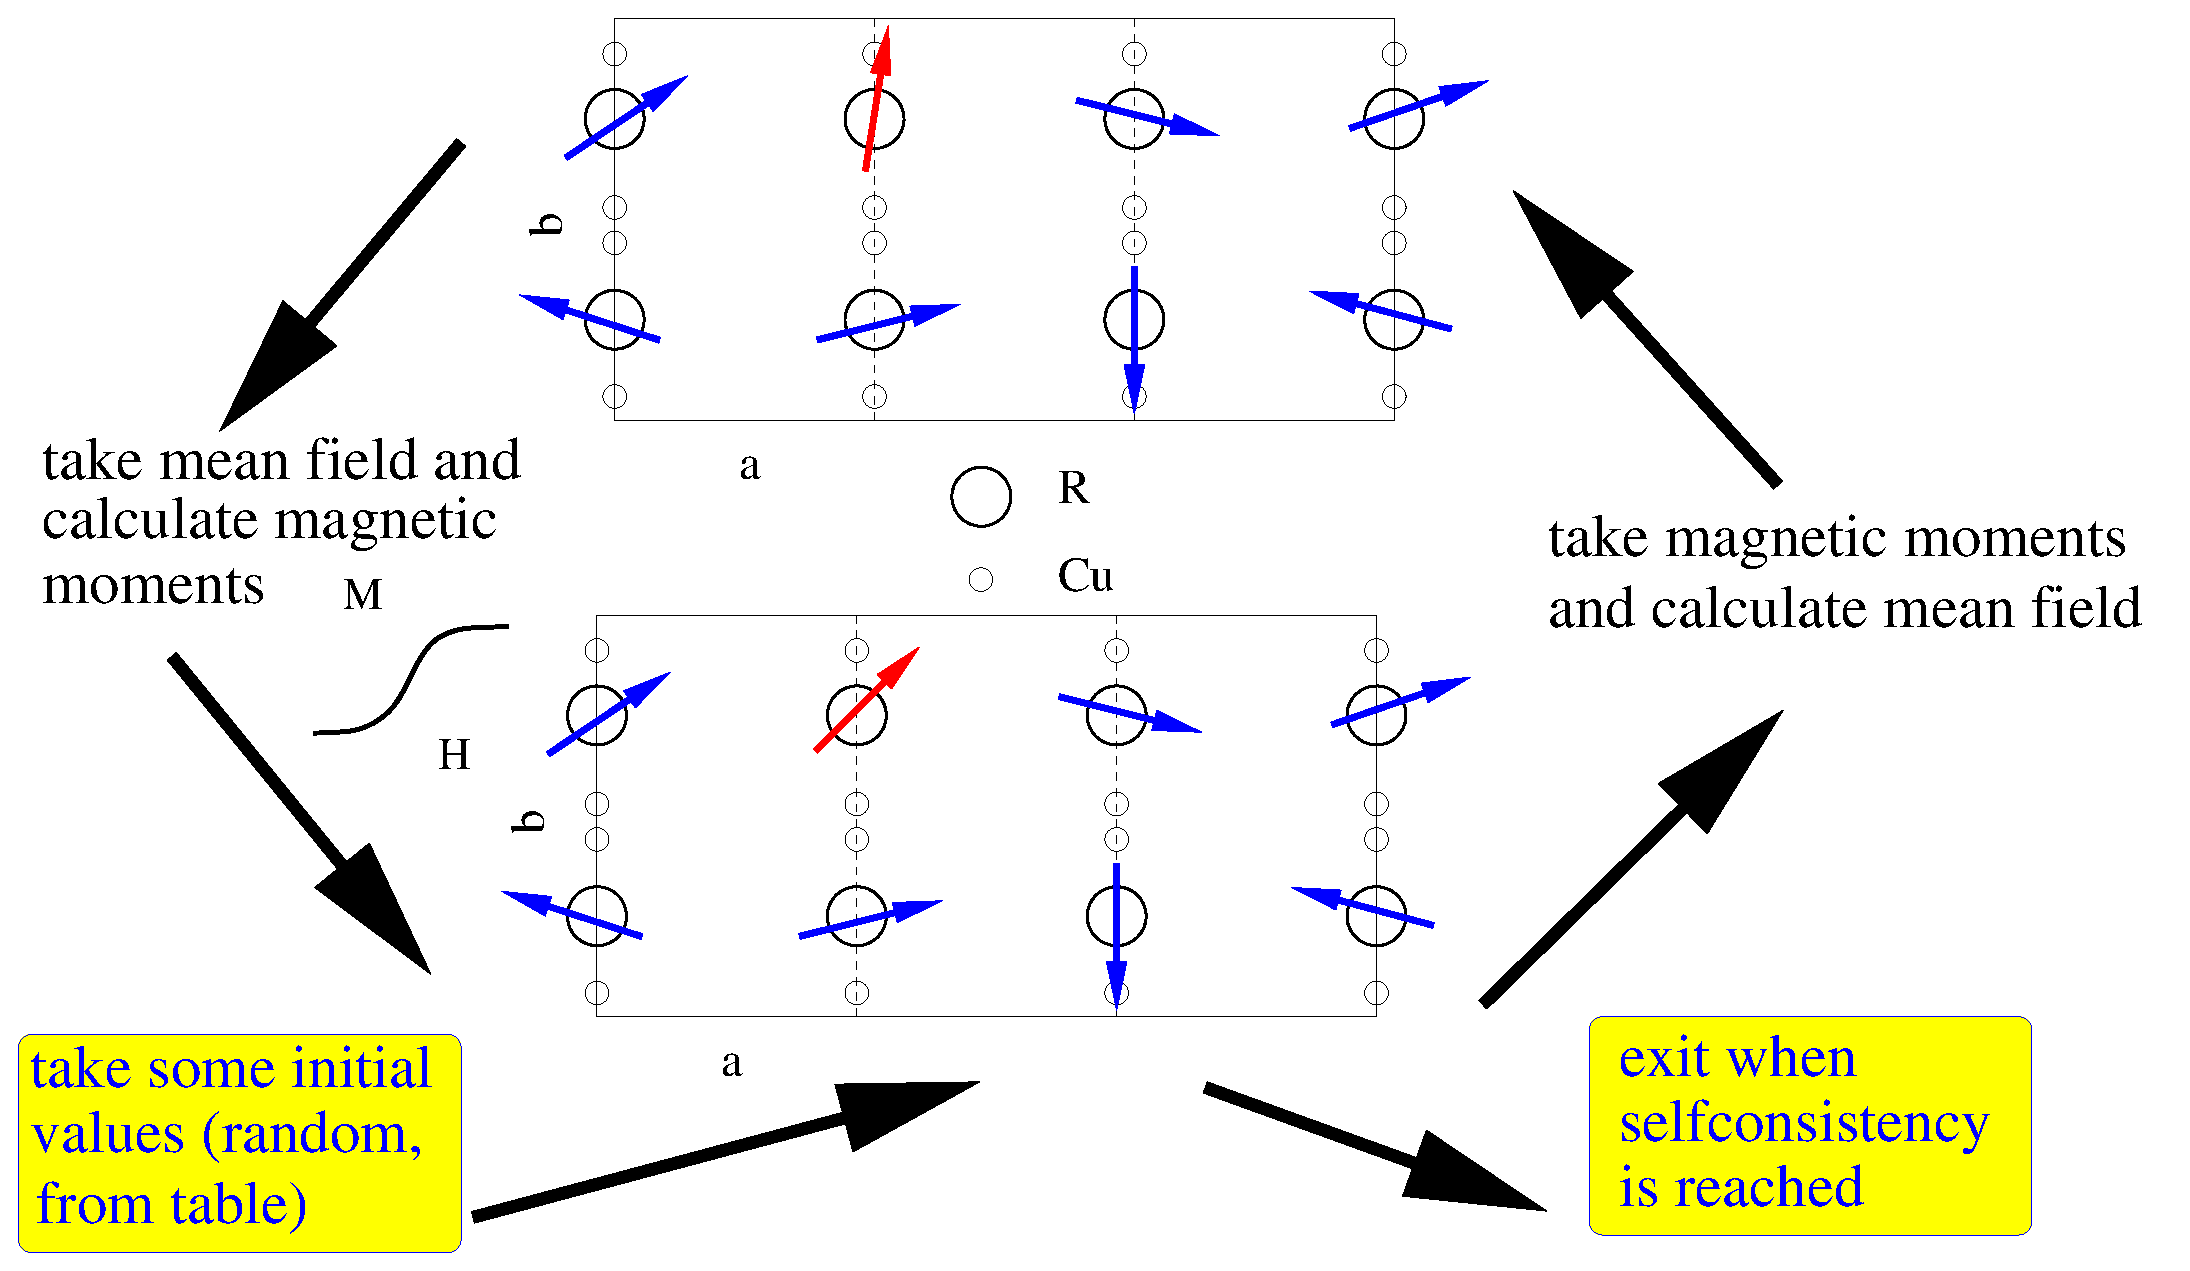
\includegraphics[angle=0,width=0.9\columnwidth]{figsrc/fecalc.eps}
\caption{\label{fecalc}Mean field process of sub {\prg fecalc}.}
\end{figure}

 
\subsubsection{Example {\prg mcphas.ini\index{mcphas.ini}} file for a simple antiferromagnet}

Here is an example of {\prg mcphas.ini\index{mcphas.ini}}, the comments describe the meaning of the different
parameters:

\input{mcphas.ini}



\subsubsection{{\prg mcphas.j\index{mcphas.j}} - lattice and exchange parameters}\label{mcphasj}
This file provides the information about 
the crystallographic
 structure and the magnetic exchange interactions.
For every atom in the crystallographic basis there
has to be given the coordinates, the number of neighbours to be considered, the 
Land\'e factor $g_J$, the single ion property filename and  a set of exchange parameters.
If the exchange parameters (and neighbour positions) are not known for your system, you 
can use the program module {\prg makenn\index{makenn}} (see section \ref{addprog}) to generate 
a list of nearest neighbours and
exchange parameters, currently implemented in {\prg makenn\index{makenn}} are dipolar interactions,
exchange interactions via the Bethe-Slater curve or the RKKY model. Note that in order
to use {\prg makenn\index{makenn}} you have to set up a working {\prg mcphas.j\index{mcphas.j}} file, which may or
may not contain neighbours and interactions.

Use program {\prg addj\index{addj}} to add exchange parameter set stored in different 
such {\prg .j} files (see section~\ref{addprog}).



\begin{description}
\item [Line 1,2:] Comment Lines
\item [Line 3:] lattice constants a,b,c and crystal angles alpha, beta, gamma 
\item [Line 4-6:] primitive lattice vectors
\item [Line 7:] Number of atoms in the primitive crystallographic unit cell ({\prg nofatoms})
\item [Line 8:] a comment line with stars
\item [Line 9:] coordinates  ($d_a$,$d_b$,$d_c$) of 1$^{st}$ magnetic ion in the crystallographic unit cell  with
respect to the lattice vectors $\vec a$,$\vec b$,$\vec c$. The number of neighbours of this 
ion, for which interaction constants are given in the interaction table (nofneighbours). 
If {\prg diagonalexchange}
is set to 0 the 9 components of the exchange tensor are given in column 4-12. 
If {\prg diagonalexchange}
 is 1, only 3 components are given (column 4-6).
If {\prg diagonalexchange}
 is 2, specific components of the exchange tensor can be given in columns 4 onwards. The indices of these components
 must be given in the following line (Line 9a below).
The Land\'e factor of the ion (gJ) and the file name of the corresponding single ion
parameter file (cffilename).
\item [Line 9a:]  If {\prg diagonalexchange=2}, then this line gives the indices of the exchange tensor corresponding to 
 the columns 4 onwards. It must have a variable called {\prg indexexchange} followed by a list of names of components of the interaction
 tensor separated by space. E.g.
 \verb|  #! indexexchange= JaJb JbJc  | 
means column 4 gives the the interaction constant between the
 first angular momentum component of the current ion with the second angular momentum component of its neighbour, whilst 
 column 5 has the interaction constant between the second angular momentum component of this ion with the third component of its
 neighbour. Alternatively, pairs of numbers may be given, as in \verb|  #! indexexchange= 1,2 2,3  |
 Additionally another parameter {\prg symmetricexchange} can be set to 1, where the value in each column is also used 
 for the transposed tensor component. Thus \verb|  #! symmetricexchange=1 indexexchange= JaJb  | is the same as \\
 \verb|  #! indexexchange= JaJb JbJa  | where the 4th and 5th column are the same.
\item [Line 10:]  Comment line
\item [Line 11-(10+nofneighbours):] Interaction table for ion number 1.   
Note: the neighbour coordinates (column 1-3) are given with respect to the lattice vectors
$\vec a$,$\vec b$,$\vec c$. The program then calculates from these values the coordinates
with respect to the primitive lattice $\vec r_1$,~$\vec r_2$,~$\vec r_3$.
($ d_a \vec a + d_b \vec b + d_c \vec c = d_1 \vec r_1 + d_2 \vec r_2 + d_3 \vec r_3$).
Column 4,5,6 \dots contain the components of the interaction tensor $\stackrel{=}{\mathcal J}$. 
Note that in case of non-orthogonal axes the 
components of the moments and the interaction tensor $Ja, Jb, Jc, Jaa, Jbb, Jcc, Jab ...$ 
refer to the orthogonal coordinate system
defined with respect to the nonorthogonal lattice $\vec a,\vec b,\vec c$ as
$Jb||\vec b$, $Jc||(\vec a \times \vec b)$ and $Ja$ perpendicular to $Jb$ and $Jc$.
\item [Line (11+nofneighbours) - end:] for each ion in the unit cell line 8 - (10+nofneighbours)
are repeated.
\end{description}


\vspace{0.5cm}

{\small {\bf Information for experienced users:}
\begin{description}
\item[\prg mcphas.jjj:]
format of exchange parameter file, which only needs a reduced set of exchange
parameters in the input file. Using the program {\prg jjj2j} the file can be transformed
to {\prg mcphas.j\index{mcphas.j}} by adding lines for all the equivalent neighbours. The format definition
of {\prg mcphas.jjj} is the same as {\prg mcphas.j\index{mcphas.j}}, however each line denotes several
equivalent neighbour atoms (instead of only one in {\prg mcphas.j\index{mcphas.j}}) according to the
 following rules:
\begin{itemize}
\item If a nonzero coordinate $d_a$ (or $d_b$,$d_c$) in the interaction table
 corresponds to it's value at the nearest
 lattice point of the primitive lattice,
  additional interactions of the same size
with  neighbours with coordinate $-d_a$ (or $-d_b$,$-d_c$, respectively)
are taken into account. This
holds for each of the three coordinates $d_a$,$d_b$ and $d_c$
 resulting in a maximum
number of 8 equivalent neighbours per line in the interaction table.
\item If the value of $d_a$ (or $d_b$,$d_c$) is zero or differs
from it's value at the nearest lattice point of the primitive lattice, it is 
changed to the value at the nearest lattice point and {\bf no} interaction 
with  neighbours with coordinates $-d_a$ (or $-d_b$,$-d_c$) is
 taken into account. If such
 interaction is needed it may be given in a different line and may
have different magnitude. In this way also crystallographic lattices
with no mirror symmetry may be described.
\end{itemize}
\item[\prg mcphas.coq:]   exchange parameters etc [ in old format]...see examples for details, use {\prg coq2jjj} to 
transform {\prg mcphas.coq} to {\prg mcphas.jjj} format
\end{description}

}


\subsubsection{Example {\prg mcphas.j\index{mcphas.j}} file for a simple antiferromagnet}

Here are example files of a tetragonal antiferromagnet with nearest neighbour interactions, all
files are equivalent:

{\small
\begin{verbatim} 
# simple antiferromagnet 
#<!--mcphase.mcphas.j-->
#***************************************************************
# Lattice Constants (A)
#! a=4.3843 b=4.3843 c=2.4194 alpha=  90 beta=  90 gamma=  90
#! r1a=   1 r2a=   0 r3a=   0
#! r1b=   0 r2b=   1 r3b=   0   primitive lattice vectors [a][b][c]
#! r1c=   0 r2c=   0 r3c=   1
#! nofatoms=1  nofcomponents=3  number of atoms in primitive unit cell/number of components of each spin
# ****************************************************************************
#! da=  0 [a] db=  0 [b] dc=  0 nofneighbours=2 diagonalexchange=0 gJ=0.857143 cffilename=Ce3p.sipf
# da[a] db[b] dc[c] Jaa[meV] Jbb[meV] Jcc[meV] Jab[meV] Jba[meV] Jac[meV] Jca[meV] Jbc[meV] Jcb[meV]
+0	+0	+1	-0.1	-0.1	-0.1   0  0  0  0  0  0
+0	+0	-1	-0.1	-0.1	-0.1   0  0  0  0  0  0
#\end{verbatim}
}

Using diagonalexchange this may be shortened to

{\small
\begin{verbatim} 
# simple antiferromagnet 
#<!--mcphase.mcphas.j-->
#***************************************************************
# Lattice Constants (A)
#! a=4.3843 b=4.3843 c=2.4194 alpha=  90 beta=  90 gamma=  90
#! r1a=   1 r2a=   0 r3a=   0
#! r1b=   0 r2b=   1 r3b=   0   primitive lattice vectors [a][b][c]
#! r1c=   0 r2c=   0 r3c=   1
#! nofatoms=1  nofcomponents=3  number of atoms in primitive unit cell/number of components of each spin
# ****************************************************************************
#! da=  0 [a] db=  0 [b] dc=  0 nofneighbours=2 diagonalexchange=1 gJ=0.857143 cffilename=Ce3p.sipf
# da[a] db[b] dc[c] Jaa[meV] Jbb[meV] Jcc[meV] Jab[meV] Jba[meV] Jac[meV] Jca[meV] Jbc[meV] Jcb[meV]
+0	+0	+1	-0.1	-0.1	-0.1   
+0	+0	-1	-0.1	-0.1	-0.1   
#\end{verbatim}
}

with indexexchange option the sequence of two ion interaction parameters can be changed and
zero parameters may be omitted:

{\small
\begin{verbatim} 
# simple antiferromagnet 
#<!--mcphase.mcphas.j-->
#***************************************************************
# Lattice Constants (A)
#! a=4.3843 b=4.3843 c=2.4194 alpha=  90 beta=  90 gamma=  90
#! r1a=   1 r2a=   0 r3a=   0
#! r1b=   0 r2b=   1 r3b=   0   primitive lattice vectors [a][b][c]
#! r1c=   0 r2c=   0 r3c=   1
#! nofatoms=1  nofcomponents=3  number of atoms in primitive unit cell/number of components of each spin
# ****************************************************************************
#! da=  0 [a] db=  0 [b] dc=  0 nofneighbours=2 diagonalexchange=2 gJ=0.857143 cffilename=Ce3p.sipf
# da[a] db[b] dc[c] Jaa[meV] Jbb[meV] Jcc[meV] Jab[meV] Jba[meV] Jac[meV] Jca[meV] Jbc[meV] Jcb[meV]
#! indexexchange = JaJa JaJc JcJa JbJb JcJc
+0	+0	+1	-0.1 0 0 -0.1	-0.1  
+0	+0	-1	-0.1 0 0 -0.1	-0.1  
#\end{verbatim}
}

{\small
\begin{verbatim} 
# simple antiferromagnet 
#<!--mcphase.mcphas.j-->
#***************************************************************
# Lattice Constants (A)
#! a=4.3843 b=4.3843 c=2.4194 alpha=  90 beta=  90 gamma=  90
#! r1a=   1 r2a=   0 r3a=   0
#! r1b=   0 r2b=   1 r3b=   0   primitive lattice vectors [a][b][c]
#! r1c=   0 r2c=   0 r3c=   1
#! nofatoms=1  nofcomponents=3  number of atoms in primitive unit cell/number of components of each spin
# ****************************************************************************
#! da=  0 [a] db=  0 [b] dc=  0 nofneighbours=2 diagonalexchange=2 gJ=0.857143 cffilename=Ce3p.sipf
# da[a] db[b] dc[c] Jaa[meV] Jbb[meV] Jcc[meV] Jab[meV] Jba[meV] Jac[meV] Jca[meV] Jbc[meV] Jcb[meV]
#! indexexchange = 1,1 1,3, 3,1 2,2 3,3
+0	+0	+1	-0.1 0 0 -0.1	-0.1  
+0	+0	-1	-0.1 0 0 -0.1	-0.1  
#\end{verbatim}
}


using symmetricexchange together with indexexchange will assume that the interaction tensor is symmetic and 
only half of it may be given:

{\small
\begin{verbatim} 
# simple antiferromagnet 
#<!--mcphase.mcphas.j-->
#***************************************************************
# Lattice Constants (A)
#! a=4.3843 b=4.3843 c=2.4194 alpha=  90 beta=  90 gamma=  90
#! r1a=   1 r2a=   0 r3a=   0
#! r1b=   0 r2b=   1 r3b=   0   primitive lattice vectors [a][b][c]
#! r1c=   0 r2c=   0 r3c=   1
#! nofatoms=1  nofcomponents=3  number of atoms in primitive unit cell/number of components of each spin
# ****************************************************************************
#! da=  0 [a] db=  0 [b] dc=  0 nofneighbours=2 diagonalexchange=2 gJ=0.857143 cffilename=Ce3p.sipf
# da[a] db[b] dc[c] Jaa[meV] Jbb[meV] Jcc[meV] Jab[meV] Jba[meV] Jac[meV] Jca[meV] Jbc[meV] Jcb[meV]
#! symmetricexchange=1 indexexchange = JaJa JaJc JbJb JcJc
+0	+0	+1	-0.1 0  -0.1	-0.1  
+0	+0	-1	-0.1 0  -0.1	-0.1  
#\end{verbatim}
}


\subsubsection{Single Ion Property Input Files}\label{sifile}

In order to speed up calculations or treat special problems a large 
variety of single ion modules is available. This includes the
option to load a user written single ion module. Details are 
given in chapter~\ref{simod}.

The first time user of {\prg McPhase} should use the module {\prg so1ion}\index{so1ion} and 
create an appropriate single ion property input file as described in
section \ref{cf1ion}. A good starting point are several examples
given in directory {\prg examples}.


\subsubsection{Example single ion property file  for a simple antiferromagnet}

Here is an example file {\prg mcphas.cf1} describing the anisotropy of a 
simple antiferromagnet with Ce atoms having basal plane anisotropy. Note the
axis convention xyz$||$abc, in case of non-orthogonal axes the convention 
is $y||\vec b$, $z||(\vec a \times \vec b)$ and $x$ perpendicular to $y$ and $z$.


\input{mcphas.cf1}

\subsubsection{{\prg mcphas.tst\index{mcphas.tst}} - input file of test spin-configurations (optional)}
This file is optional and contains
some test momentum configurations to be used for the calculation
             of the free energy. Mind that
\begin{itemize}
\item  in the file header the number of atoms in the primitive
       crystallographic unit cell and the number of components
       of the spin vector have to be given.
\item  at the end of the
 file there must be no empty lines !
\end{itemize}

The momentum - configurations tables always refer to spins sitting on
the primitive lattice ${\mbf r}_i$. If more than one atom is in
the primitive basis, the momentum gets $3n$ components ($n=$ number
of atoms in the crystallographic basis). See {\prg ./examples/ndcu2b\_new/} for
examples of a two atom basis. Units of these tables are that of total 
angular momentum $<J>$.

\subsubsection{Example {\prg mcphas.tst\index{mcphas.tst}} file  for a simple antiferromagnet}

Here is the file {\prg mcphas.tst\index{mcphas.tst}} for the simple antiferromagnet example
describing some spin configurations
to be used as starting values for the mean field process:

\input{mcphas.tst}
Note, in case of non-orthogonal axes the convention 
is $mb||\vec b$, $mc||(\vec a \times \vec b)$ and $ma$ perpendicular to $mb$ and $mc$.

\subsubsection{subdirectory {\prg ./results} - directory where calculated data is stored}

In order to be able to save the results of a calculation the directory {\prg ./results} has to
exist. Mind that all files in this directory will be overwritten without warning. 

\subsubsection{subdirectory {\prg ./fit} - experimental data for fit (optional) } 

In order that {\prg McPhase} can calculate the standard deviation between
 experimental data and the results of the simulation, some experimental data
 can be given in the subdirectory {\prg ./fit}. The filenames and the data-format
 are the same as the output files of {\prg McPhas}, e.g. {\prg mcphas.fum}, {\prg mcphas.hkl}
 etc. {\prg McPhase} looks into the directory {\prg ./fit} and if it finds any
 of these files, the standard deviation is increased correspondingly. 

What measurement data can be used to calculate a standard deviation ?

\begin{description}
\item[{\prg mcphas.fum}] if given in column 11, 12, 13 in {\prg ./fit/mcphas.fum} the
            magnetisation in the $a$, $b$ and $c$ direction is used for calculation
	    of the standard deviation sta. The standard deviation is calculated
	    as ${\rm sta}=\sum_{\rm data points i} ({\mbf m}_i^{calc}-{\mbf m}_i^{meas})^2$.
	    All three components of the magnetic moment have to be given and are used.

\end{description}

Note that the measured data has to be given in those (H-T) points which are 
calculated by mcphas\index{mcphas} in order to be used by the program to increase {\prg sta}.
It is usually most effective to fit only few data points, because a large set
of data points will not improve the quality of the fit and only require a large
amount of calculation time.



\subsection{Starting a simulation}
\label{start}

To start the simulation goto the directory containing the
input files {\prg mcphas.ini, mcphas.j, etc. } and type

\begin{description}
\item[\prg mcphas] to run the program generating stepwise $H-T$ values 
              in a loop given by {\prg mcphas.ini\index{mcphas.ini}} (you can also press the
              symbol in the {\prg McPhase - Explorer} window).
\item[\prg mcphas\index{mcphas} [file]]  to run the program with an input file --   
             {\prg file} contains T ha hb hc values to be calculated 
             if [file] is not given, xmin xmax xstep (xT xHa xHb xHc)
             ymin ymax ystep (yT yHa yHb yHc) is read from file {\prg mcphas.ini\index{mcphas.ini}}
	     and phase diagram is calculated
\item[\prg mcphas\index{mcphas} -h]  to  print help and version of {\prg McPhas}.
\item[\prg mcphas\index{mcphas} -stamax 14]  end mcphas\index{mcphas} if standard deviation exceeds 14.
\item[\prg mcphas\index{mcphas} -a] avoid overwriting output files in results, append new results to existing files
\item[\prg mcphas\index{mcphas} -v]  to  enable verbose mode with lots of messages of {\prg McPhas}. Specifically
the verbose mode enables the following features:
  \begin{itemize}
			          \item more information is printed out, 
			          \item the q-vectors file {\prg ./results/mcphas.qvc} will contain 
				    the explicit spin configurations
			          \item the display\index{display} on screen (ghostview window using 
				     {\prg ./results/.sps.eps}) will be updated not only 
				    when a H-T point has been finished but always 
				    when a structure with smaller free energy 
				    has been stabilised
  \end{itemize}
\item[\prg mcphasit\index{mcphas}] to start mcphase in commandline mode without opening any window
\end{description}

\vspace{1cm}
{\em Exercises:}
\begin{itemize}
\item Look at the input files for {\prg McPhase} given in the directory
{\prg examples/ndcu2b\_new}.  How many atoms are contained in the crystallographic basis ?
\item
Start the simulation by typing the command {\prg mcphas}.
\end{itemize}



\subsection{Options for a running simulation}
... when the program is running, the options in the main window
can be changed. Pressing ''displayall'' displays the current spin-configuration
at each iteration step. Pressing ''log fe vs Q'' appends free energy vs Q
data to {\prg mcphas.log} for every ($T-H$) point.


The file {\prg ./results/.spins.eps} is used to show the information about the currently calculated
spin structure on the screen using the postscript file viewer ghostview.

The file {\prg ./results/.mcphas.fum} contains the information of the magnetisation curve
which is currently calculated. This information is automatically displayed on the screen.


The program {\prg display} (see section \ref{display}) can be used 
for the online display\index{display} of any other
curve(s).


\subsection{Output Files - {\prg mcphas.qvc,phs,sps,mf,fum,j1...,xyt,hkl} }\label{outputfiles}
 (in directory ./results/ after a simulation run) 

\begin{figure}[htb]%h=here, t=top, b=bottom, p=separate figure page
\begin{center}\leavevmode
\includegraphics[angle=0, width=0.3\textwidth]{figsrc/magnetization_ndcu2.ps}
\end{center}
\caption{Calculated magnetisation of NdCu$_2$ for field parallel to the orthorhombic $b$-direction.}
\label{magnetization}
\end{figure}

\begin{figure}[htb]%h=here, t=top, b=bottom, p=separate figure page
\begin{center}\leavevmode
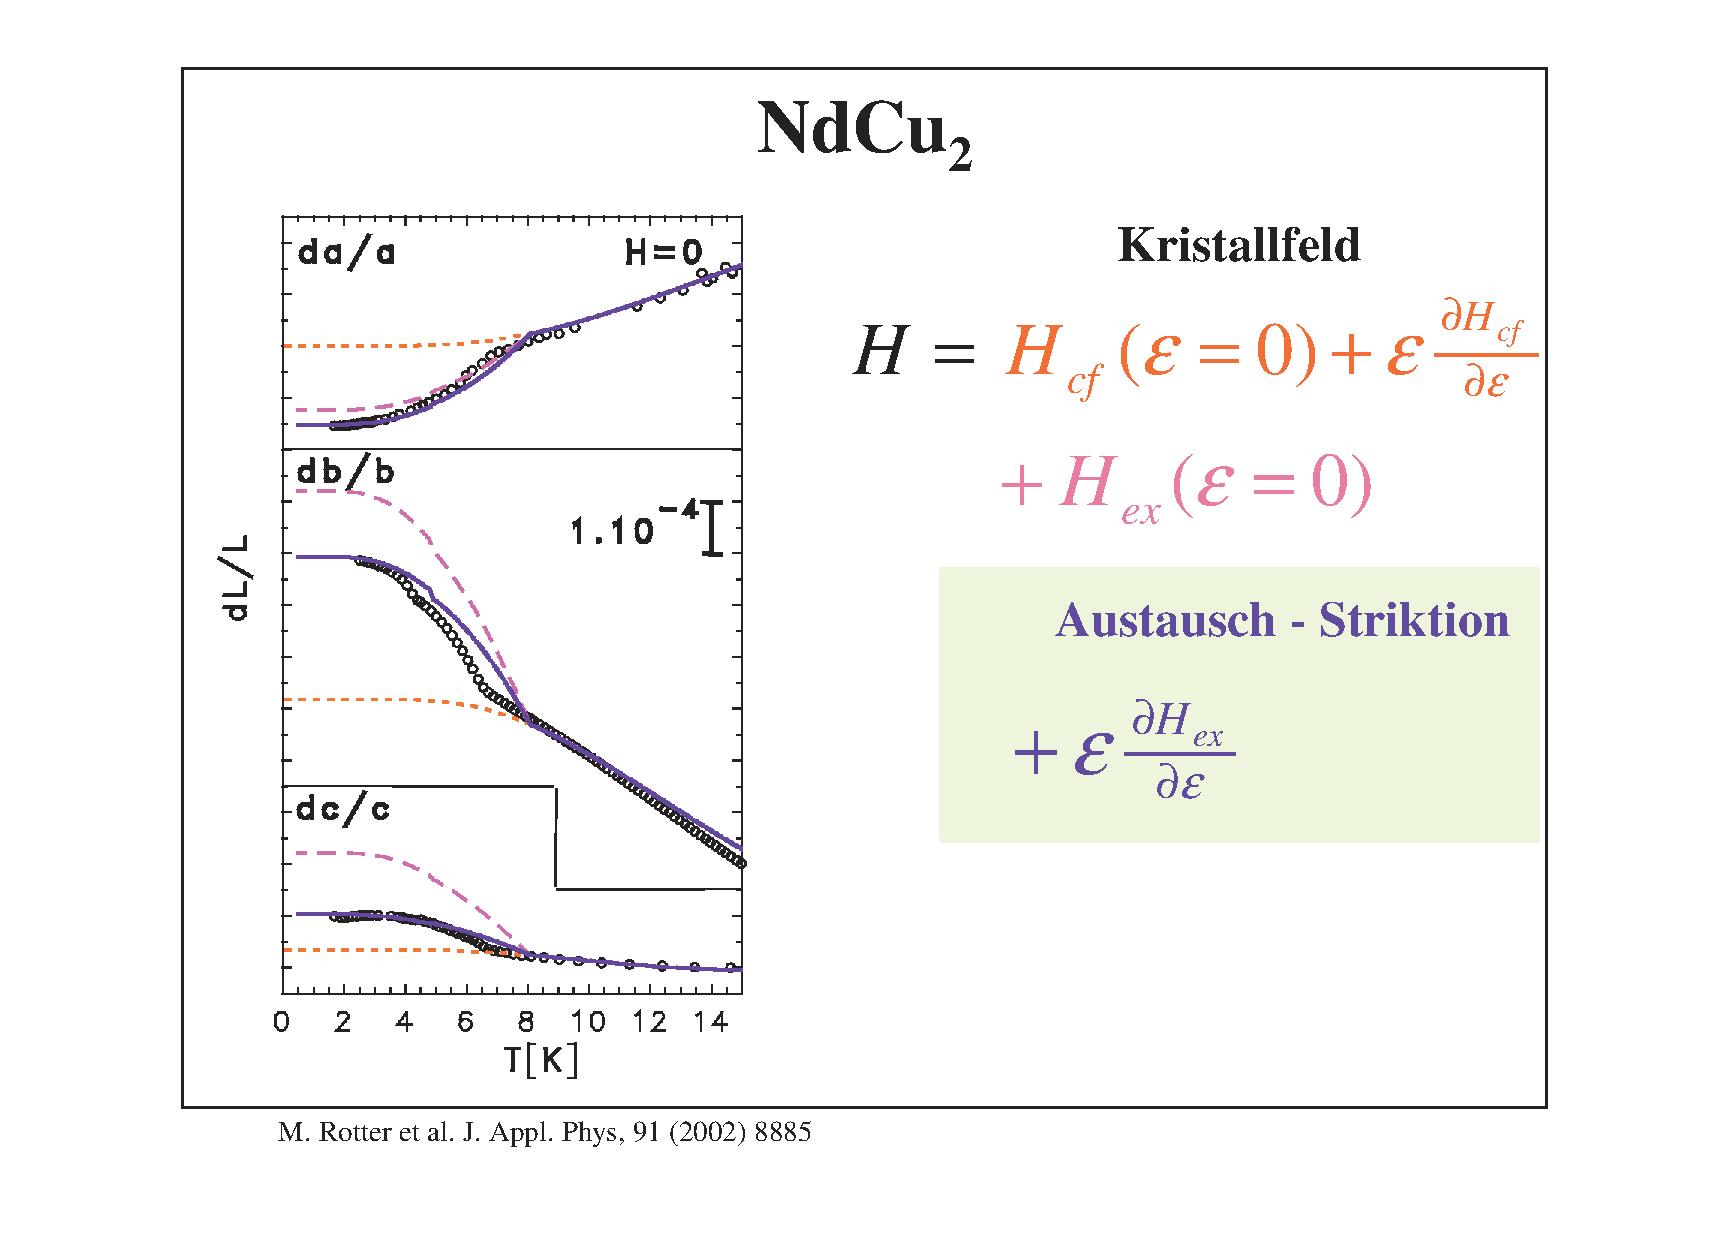
\includegraphics[angle=0, width=0.8\textwidth]{figsrc/magnetostriction_ndcu2.eps}
\end{center}
\caption{Calculated spontaneous magnetostriction of NdCu$_2$.}
\label{magnetostrictiongraphic}
\end{figure}

\begin{description}
\item [\prg mcphas.qvc]    the set of test q-vectors used for calculation of free energy.
                           Components of these q vectors refer to the reciprocal lattice $\vec a^*,\vec b^*,\vec c^*$.
\item [\prg mcphas.phs]    spin-configuration table of different types of spin-configurations. 
                            Note, in case of non-orthogonal axes the convention in these tables 
                            is $mb||\vec b$, $mc||(\vec a \times \vec b)$ and $ma$ perpendicular to $mb$ and $mc$.

                           {\em Note}: 
                           there is no natural criteria for deciding, if one spin-configuration is
			   different from another one. Therefore the list of ''different''
			   spin-configurations is dependent on the meaning of ''different''.
			   
			   The program {\prg McPhase} decides whether a spin-configuration is
			   different from another by a simple criteria, namely by the
			   angle between the spins. Comparing two spin configurations it calculates
			   the angle between corresponding spins and if for one spin the
			   angle is not small, the configuration is treated as a different
			   configuration. Therefore for example a ferromagnet with moments
			   in $a$ has a different spin configuration than a ferromagnet with
			   moments in $b$ direction. 
\item [\prg mcphas.sps]    $T-H$ dependence of spin-configuration. The spin configurations stored in this
                           file may be displayed using the program {\prg spins\index{spins}}, an example is given
			   in figure~\ref{spingraphic}.
                            Note, in case of non-orthogonal axes the convention for applied field $Ha, Hb,Hc$ and
                            also for the moment components $ma, mb, mc$ in these tables 
                            is $mb||\vec b$, $mc||(\vec a \times \vec b)$ and $ma$ perpendicular to $mb$ and $mc$.

\item [\prg mcphas.mf]     $T-H$ dependence of exchange field configuration, stored as $g_J \mu_B H_{xc}(i)$(unit is in meV)
                            for i=1,2,...,number of spins in magnetic unit cell.
                            Note, in case of non-orthogonal axes the convention for applied field $Ha, Hb,Hc$ and
                            also for the mean field components in these tables 
                            is $Hb||\vec b$, $Hc||(\vec a \times \vec b)$ and $Ha$ perpendicular to $Hb$ and $Hc$.
\item [\prg mcphas.fum]    free energy, magnetic energy (the derivative with respect to temperature gives the specific %%@
heat),
                           magnetisation data and (if cfield is used with higher order interactions)
                           expectation values of the Stevens Operators $<O_l^m>$ . As an example for the information
			   contained in this file the calculated magnetisation and magnetostriction of NdCu$_2$ is shown in
			   figures~\ref{magnetization} and ~\ref{magnetizationgraphic}.
                            Note, in case of non-orthogonal axes the convention for applied field $Ha, Hb,Hc$ and
                            also for the magnetisation components $ma,mb,mc$ in these tables 
                            is $Hb||\vec b$, $Hc||(\vec a \times \vec b)$ and $Ha$ perpendicular to $Hb$ and $Hc$.

\item [\prg mcphas1.j1 .j1 .j2 ...] 
               spin-spin correlation functions for sub-lattice 1 neighbour 1 2 ...
	       (linear combination is proportional to magnetostriction)
	       The spin-spin correlation functions for neighbour $k$ are defined by
	       the following sum of dyadic products:

	       \begin{equation}
	        \frac{1}{n}\sum_{s=1}^n <{\mbf J}^s> \times  <{\mbf J}^{s+k}>
	       \end{equation}
	       with $n$ being the number of moments in the magnetic unit cell.
	       Single ion and two-ion magnetostriction can be calculated using the $<O_l^m>$ and the
	       spin-spin correlation functions. As an example the magnetostriction analysis of
	       NdCu$_2$ is shown in figure~\ref{magnetostrictiongraphic}. For details 
             please refer to~\cite{rotter02-8885}.
                            Note, in case of non-orthogonal axes the convention for applied field $Ha, Hb,Hc$ and
                            also for the moment components in these tables 
                            is $Hb||\vec b$, $Hc||(\vec a \times \vec b)$ and $Ha$ perpendicular to $Hb$ and $Hc$.
\item [\prg mcphas.xyt]    phase diagram as x,y,T, H, phase-number j according to spin-configuration table
               given in mcphas.phs, a periodicity key, nettomoments <J>.
 Figure~\ref{phasediagramgraphic}
	       shows the phase diagram of NdCu$_2$ for magnetic fields parallel to the orthorhombic $b$-direction.
                            Note, in case of non-orthogonal axes the convention for applied field $Ha, Hb,Hc$ 
                             in these tables 
                            is $Hb||\vec b$, $Hc||(\vec a \times \vec b)$ and $Ha$ perpendicular to $Hb$ and $Hc$.
\item [\prg mcphas.hkl]    calculated (unpolarised) neutron diffraction data (the calculated magnetic intensities
    correspond to the magnetic structure + Polarisation factor. The
    Lorentz-factor , magnetic form factor and  instrumental corrections are not calculated.)
 As an example figure~\ref{neutintgraphic}
    shows the calculated temperature dependence of magnetic amplitudes for NdCu$_2$.
                           $h,k,l$ refer to the reciprocal lattice $\vec a^*,\vec b^*,\vec c^*$.
                            Note, in case of non-orthogonal axes the convention for applied field $Ha, Hb,Hc$ 
                             in these tables 
                            is $Hb||\vec b$, $Hc||(\vec a \times \vec b)$ and $Ha$ perpendicular to $Hb$ and $Hc$.
    
\item [\prg mcphasa.hkl]    Fourier Transform of the $a$-component of the magnetic Moments.
                           $h,k,l$ refer to the reciprocal lattice $\vec a^*,\vec b^*,\vec c^*$.
                            Note, in case of non-orthogonal axes the convention for applied field $Ha, Hb,Hc$ and
                            the magnetic moment component in these tables 
                            is $Hb||\vec b$, $Hc||(\vec a \times \vec b)$ and $Ha$ perpendicular to $Hb$ and $Hc$.
\item [\prg mcphasb.hkl]    Fourier Transform of the $b$-component of the magnetic Moments.
                           $h,k,l$ refer to the reciprocal lattice $\vec a^*,\vec b^*,\vec c^*$.
                            Note, in case of non-orthogonal axes the convention for applied field $Ha, Hb,Hc$ and
                            the magnetic moment component in these tables 
                            is $Hb||\vec b$, $Hc||(\vec a \times \vec b)$ and $Ha$ perpendicular to $Hb$ and $Hc$.
\item [\prg mcphasc.hkl]    Fourier Transform of the $c$-component of the magnetic Moments.
                           $h,k,l$ refer to the reciprocal lattice $\vec a^*,\vec b^*,\vec c^*$.
                            Note, in case of non-orthogonal axes the convention for applied field $Ha, Hb,Hc$ and
                            the magnetic moment component in these tables 
                            is $Hb||\vec b$, $Hc||(\vec a \times \vec b)$ and $Ha$ perpendicular to $Hb$ and $Hc$.
\end{description} 

\vspace{1cm}
{\em Exercises:}
\begin{itemize}
\item Look at the output files of {\prg McPhase}  in the directory
{\prg examples/ndcu2b\_new/results}.  At which magnetic field
the ferromagnetically aligned state is achieved (at $T=$2~K)?
\item
What is the propagation vector in the different antiferromagnetic phases at $T=$2~K ?
\end{itemize}





\subsubsection{{\prg mcphas.j\index{mcphas.j}} - lattice and exchange parameters}\label{mcphasj}
This file provides the information about 
the crystallographic
 structure and the magnetic exchange interactions.
For every atom in the crystallographic basis there
has to be given the coordinates, the number of neighbours to be considered, the 
Land\'e factor $g_J$, the single ion property filename and  a set of exchange parameters.
If the exchange parameters (and neighbour positions) are not known for your system, you 
can use the program module {\prg makenn\index{makenn}} (see section \ref{addprog}) to generate 
a list of nearest neighbours and
exchange parameters, currently implemented in {\prg makenn\index{makenn}} are dipolar interactions,
exchange interactions via the Bethe-Slater curve or the RKKY model. Note that in order
to use {\prg makenn\index{makenn}} you have to set up a working {\prg mcphas.j\index{mcphas.j}} file, which may or
may not contain neighbours and interactions.

Use program {\prg addj\index{addj}} to add exchange parameter set stored in different 
such {\prg .j} files (see section~\ref{addprog}).



\begin{description}
\item [Line 1,2:] Comment Lines
\item [Line 3:] lattice constants a,b,c and crystal angles alpha, beta, gamma 
\item [Line 4-6:] primitive lattice vectors
\item [Line 7:] Number of atoms in the primitive crystallographic unit cell ({\prg nofatoms})
\item [Line 8:] a comment line with stars
\item [Line 9:] coordinates  ($d_a$,$d_b$,$d_c$) of 1$^{st}$ magnetic ion in the crystallographic unit cell  with
respect to the lattice vectors $\vec a$,$\vec b$,$\vec c$. The number of neighbours of this 
ion, for which interaction constants are given in the interaction table (nofneighbours). 
If {\prg diagonalexchange}
is set to 0 the 9 components of the exchange tensor are given in column 4-12. 
If {\prg diagonalexchange}
 is 1, only 3 components are given (column 4-6).
If {\prg diagonalexchange}
 is 2, specific components of the exchange tensor can be given in columns 4 onwards. The indices of these components
 must be given in the following line (Line 9a below).
The Land\'e factor of the ion (gJ) and the file name of the corresponding single ion
parameter file (cffilename).
\item [Line 9a:]  If {\prg diagonalexchange=2}, then this line gives the indices of the exchange tensor corresponding to 
 the columns 4 onwards. It must have a variable called {\prg indexexchange} followed by a list of names of components of the interaction
 tensor separated by space. E.g.
 \verb|  #! indexexchange= JaJb JbJc  | 
means column 4 gives the the interaction constant between the
 first angular momentum component of the current ion with the second angular momentum component of its neighbour, whilst 
 column 5 has the interaction constant between the second angular momentum component of this ion with the third component of its
 neighbour. Alternatively, pairs of numbers may be given, as in \verb|  #! indexexchange= 1,2 2,3  |
 Additionally another parameter {\prg symmetricexchange} can be set to 1, where the value in each column is also used 
 for the transposed tensor component. Thus \verb|  #! symmetricexchange=1 indexexchange= JaJb  | is the same as \\
 \verb|  #! indexexchange= JaJb JbJa  | where the 4th and 5th column are the same.
\item [Line 10:]  Comment line
\item [Line 11-(10+nofneighbours):] Interaction table for ion number 1.   
Note: the neighbour coordinates (column 1-3) are given with respect to the lattice vectors
$\vec a$,$\vec b$,$\vec c$. The program then calculates from these values the coordinates
with respect to the primitive lattice $\vec r_1$,~$\vec r_2$,~$\vec r_3$.
($ d_a \vec a + d_b \vec b + d_c \vec c = d_1 \vec r_1 + d_2 \vec r_2 + d_3 \vec r_3$).
Column 4,5,6 \dots contain the components of the interaction tensor $\stackrel{=}{\mathcal J}$. 
Note that in case of non-orthogonal axes the 
components of the moments and the interaction tensor $Ja, Jb, Jc, Jaa, Jbb, Jcc, Jab ...$ 
refer to the orthogonal coordinate system
defined with respect to the nonorthogonal lattice $\vec a,\vec b,\vec c$ as
$Jb||\vec b$, $Jc||(\vec a \times \vec b)$ and $Ja$ perpendicular to $Jb$ and $Jc$.
\item [Line (11+nofneighbours) - end:] for each ion in the unit cell line 8 - (10+nofneighbours)
are repeated.
\end{description}


\vspace{0.5cm}

{\small {\bf Information for experienced users:}
\begin{description}
\item[\prg mcphas.jjj:]
format of exchange parameter file, which only needs a reduced set of exchange
parameters in the input file. Using the program {\prg jjj2j} the file can be transformed
to {\prg mcphas.j\index{mcphas.j}} by adding lines for all the equivalent neighbours. The format definition
of {\prg mcphas.jjj} is the same as {\prg mcphas.j\index{mcphas.j}}, however each line denotes several
equivalent neighbour atoms (instead of only one in {\prg mcphas.j\index{mcphas.j}}) according to the
 following rules:
\begin{itemize}
\item If a nonzero coordinate $d_a$ (or $d_b$,$d_c$) in the interaction table
 corresponds to it's value at the nearest
 lattice point of the primitive lattice,
  additional interactions of the same size
with  neighbours with coordinate $-d_a$ (or $-d_b$,$-d_c$, respectively)
are taken into account. This
holds for each of the three coordinates $d_a$,$d_b$ and $d_c$
 resulting in a maximum
number of 8 equivalent neighbours per line in the interaction table.
\item If the value of $d_a$ (or $d_b$,$d_c$) is zero or differs
from it's value at the nearest lattice point of the primitive lattice, it is 
changed to the value at the nearest lattice point and {\bf no} interaction 
with  neighbours with coordinates $-d_a$ (or $-d_b$,$-d_c$) is
 taken into account. If such
 interaction is needed it may be given in a different line and may
have different magnitude. In this way also crystallographic lattices
with no mirror symmetry may be described.
\end{itemize}
\item[\prg mcphas.coq:]   exchange parameters etc [ in old format]...see examples for details, use {\prg coq2jjj} to 
transform {\prg mcphas.coq} to {\prg mcphas.jjj} format
\end{description}

}


\subsubsection{Example {\prg mcphas.j\index{mcphas.j}} file for a simple antiferromagnet}

Here are example files of a tetragonal antiferromagnet with nearest neighbour interactions, all
files are equivalent:

{\small
\begin{verbatim} 
# simple antiferromagnet 
#<!--mcphase.mcphas.j-->
#***************************************************************
# Lattice Constants (A)
#! a=4.3843 b=4.3843 c=2.4194 alpha=  90 beta=  90 gamma=  90
#! r1a=   1 r2a=   0 r3a=   0
#! r1b=   0 r2b=   1 r3b=   0   primitive lattice vectors [a][b][c]
#! r1c=   0 r2c=   0 r3c=   1
#! nofatoms=1  nofcomponents=3  number of atoms in primitive unit cell/number of components of each spin
# ****************************************************************************
#! da=  0 [a] db=  0 [b] dc=  0 nofneighbours=2 diagonalexchange=0 gJ=0.857143 cffilename=Ce3p.sipf
# da[a] db[b] dc[c] Jaa[meV] Jbb[meV] Jcc[meV] Jab[meV] Jba[meV] Jac[meV] Jca[meV] Jbc[meV] Jcb[meV]
+0	+0	+1	-0.1	-0.1	-0.1   0  0  0  0  0  0
+0	+0	-1	-0.1	-0.1	-0.1   0  0  0  0  0  0
#\end{verbatim}
}

Using diagonalexchange this may be shortened to

{\small
\begin{verbatim} 
# simple antiferromagnet 
#<!--mcphase.mcphas.j-->
#***************************************************************
# Lattice Constants (A)
#! a=4.3843 b=4.3843 c=2.4194 alpha=  90 beta=  90 gamma=  90
#! r1a=   1 r2a=   0 r3a=   0
#! r1b=   0 r2b=   1 r3b=   0   primitive lattice vectors [a][b][c]
#! r1c=   0 r2c=   0 r3c=   1
#! nofatoms=1  nofcomponents=3  number of atoms in primitive unit cell/number of components of each spin
# ****************************************************************************
#! da=  0 [a] db=  0 [b] dc=  0 nofneighbours=2 diagonalexchange=1 gJ=0.857143 cffilename=Ce3p.sipf
# da[a] db[b] dc[c] Jaa[meV] Jbb[meV] Jcc[meV] Jab[meV] Jba[meV] Jac[meV] Jca[meV] Jbc[meV] Jcb[meV]
+0	+0	+1	-0.1	-0.1	-0.1   
+0	+0	-1	-0.1	-0.1	-0.1   
#\end{verbatim}
}

with indexexchange option the sequence of two ion interaction parameters can be changed and
zero parameters may be omitted:

{\small
\begin{verbatim} 
# simple antiferromagnet 
#<!--mcphase.mcphas.j-->
#***************************************************************
# Lattice Constants (A)
#! a=4.3843 b=4.3843 c=2.4194 alpha=  90 beta=  90 gamma=  90
#! r1a=   1 r2a=   0 r3a=   0
#! r1b=   0 r2b=   1 r3b=   0   primitive lattice vectors [a][b][c]
#! r1c=   0 r2c=   0 r3c=   1
#! nofatoms=1  nofcomponents=3  number of atoms in primitive unit cell/number of components of each spin
# ****************************************************************************
#! da=  0 [a] db=  0 [b] dc=  0 nofneighbours=2 diagonalexchange=2 gJ=0.857143 cffilename=Ce3p.sipf
# da[a] db[b] dc[c] Jaa[meV] Jbb[meV] Jcc[meV] Jab[meV] Jba[meV] Jac[meV] Jca[meV] Jbc[meV] Jcb[meV]
#! indexexchange = JaJa JaJc JcJa JbJb JcJc
+0	+0	+1	-0.1 0 0 -0.1	-0.1  
+0	+0	-1	-0.1 0 0 -0.1	-0.1  
#\end{verbatim}
}

{\small
\begin{verbatim} 
# simple antiferromagnet 
#<!--mcphase.mcphas.j-->
#***************************************************************
# Lattice Constants (A)
#! a=4.3843 b=4.3843 c=2.4194 alpha=  90 beta=  90 gamma=  90
#! r1a=   1 r2a=   0 r3a=   0
#! r1b=   0 r2b=   1 r3b=   0   primitive lattice vectors [a][b][c]
#! r1c=   0 r2c=   0 r3c=   1
#! nofatoms=1  nofcomponents=3  number of atoms in primitive unit cell/number of components of each spin
# ****************************************************************************
#! da=  0 [a] db=  0 [b] dc=  0 nofneighbours=2 diagonalexchange=2 gJ=0.857143 cffilename=Ce3p.sipf
# da[a] db[b] dc[c] Jaa[meV] Jbb[meV] Jcc[meV] Jab[meV] Jba[meV] Jac[meV] Jca[meV] Jbc[meV] Jcb[meV]
#! indexexchange = 1,1 1,3, 3,1 2,2 3,3
+0	+0	+1	-0.1 0 0 -0.1	-0.1  
+0	+0	-1	-0.1 0 0 -0.1	-0.1  
#\end{verbatim}
}


using symmetricexchange together with indexexchange will assume that the interaction tensor is symmetic and 
only half of it may be given:

{\small
\begin{verbatim} 
# simple antiferromagnet 
#<!--mcphase.mcphas.j-->
#***************************************************************
# Lattice Constants (A)
#! a=4.3843 b=4.3843 c=2.4194 alpha=  90 beta=  90 gamma=  90
#! r1a=   1 r2a=   0 r3a=   0
#! r1b=   0 r2b=   1 r3b=   0   primitive lattice vectors [a][b][c]
#! r1c=   0 r2c=   0 r3c=   1
#! nofatoms=1  nofcomponents=3  number of atoms in primitive unit cell/number of components of each spin
# ****************************************************************************
#! da=  0 [a] db=  0 [b] dc=  0 nofneighbours=2 diagonalexchange=2 gJ=0.857143 cffilename=Ce3p.sipf
# da[a] db[b] dc[c] Jaa[meV] Jbb[meV] Jcc[meV] Jab[meV] Jba[meV] Jac[meV] Jca[meV] Jbc[meV] Jcb[meV]
#! symmetricexchange=1 indexexchange = JaJa JaJc JbJb JcJc
+0	+0	+1	-0.1 0  -0.1	-0.1  
+0	+0	-1	-0.1 0  -0.1	-0.1  
#\end{verbatim}
}


\subsubsection{Single Ion Property Input Files}\label{sifile}

In order to speed up calculations or treat special problems a large 
variety of single ion modules is available. This includes the
option to load a user written single ion module. Details are 
given in chapter~\ref{simod}.

The first time user of {\prg McPhase} should use the module {\prg so1ion}\index{so1ion} and 
create an appropriate single ion property input file as described in
section \ref{cf1ion}. A good starting point are several examples
given in directory {\prg examples}.


\subsubsection{Example single ion property file  for a simple antiferromagnet}

Here is an example file {\prg mcphas.cf1} describing the anisotropy of a 
simple antiferromagnet with Ce atoms having basal plane anisotropy. Note the
axis convention xyz$||$abc, in case of non-orthogonal axes the convention 
is $y||\vec b$, $z||(\vec a \times \vec b)$ and $x$ perpendicular to $y$ and $z$.


\section{{\prg mcphas} - calculation of thermodynamic properties (Magnetisation, Susceptibility, Specific Heat, Neutron %%@
Diffraction, etc.)}
\label{runmcphas}

In order to perform calculations beyond the capabilities of {\prg cfield\index{cfield}} it is necessary
to use the program {\prg mcphas}. 
\begin{itemize}
\item As a first step it is possible to
calculate the thermodynamic properties such as magnetisation or specific heat
considering only single ion effects. In this case all the exchange parameters
have to be set to zero in {\prg mcphas.j\index{mcphas.j}}. 
\item for more advanced calculations the two - ion interactions have to be
considered and may lead to magnetic order. {\prg mcphas} can perform 
calculations in the ordered state in the following way: for 
a given temperature $T$ and magnetic field $\mbf H$ (vector)
several possible magnetic structures are stabilised
by a mean field algorithm and the free energy is 
calculated. The initial values for this mean-field procedure are
modified by a Monte Carlo process.


The temperature and magnetic field is varied during the calculation
and thereby it is possible to map out the magnetic phase diagram.
\end{itemize}

The program produces a plot of the stabilised magnetic
structures and the magnetisation on screen, the
output files contain additional information 
such as calculated magnetoelastic and  neutron-scattering
data. Several graphic programs easy the visualisation of the
calculated data (section~\ref{graphics}).



\subsection{Input Files}
The program {\prg McPhase} needs the following input files (all in the same directory)
 in order to run:

\begin{enumerate}
\item {\prg mcphas.ini\index{mcphas.ini}}
 - controlling the algorithm
\item {\prg mcphas.j\index{mcphas.j}}
  - lattice and exchange parameters
\item {\prg mcphas.tst\index{mcphas.tst}(optional)}  - test spin configurations
\item {\prg single-ion property files}
\item {\prg directory ./results/}
 - directory where calculated data is stored
\item {\prg directory ./fit} - experimental data for fit (optional)
\end{enumerate}


 All
 of these input files have to be in one directory and the program
has to be started in this directory. The results of the simulation
are then stored in the  subdirectory ./results/, which must exist before starting
the program 
... see directory ./examples/ for some examples.
 In order to prepare these files
for a new calculation it is best to take them from an example, copy the files
to a new directory and make the
modifications  to adapt them to the new problem.

\subsubsection{Example - a simple antiferromagnet}

In the following description of the input files we will always refer
to a simple example: a simple antiferromagnet
on a primitive orthorhombic lattice. The first time user
will thus have a simple example to follow, all corresponding
files are given in the directory {\prg tutorial/03magnetic\_phases\_mcphas/simpleAF}.
 

\subsubsection{{\prg mcphas.ini\index{mcphas.ini}} - controlling the algorithm}
   Initial file containing algorithm control parameters, for instance the range and spacing of
   propagation vectors Q or the number of Monte Carlo trials for initial spin configurations
    - {\em mind}: this
   file is rewritten and reread  when running the program and may be changed by the
   user in order to manipulate the running simulation.

{\prg mcphas.ini\index{mcphas.ini}} consists of several sections:
\begin{description}
\item [MCPHASE RUNTIME CONTROL:] this section contains the parameters
controlling the status of the calculation.
\item [XY PHASEDIAGRAM PARAMETERS:] here the temperature and field range and
step widths of the calculation are specified.
The definition of the x and y
axis in terms of temperature and magnetic field is followed by the
corresponding range and step width. An offset may be given for all
field and temperature values.
Note that for most cases of interest
this offset is zero (T0=0, Ha0=0, Hb0=0, Hc0=0).
 For the simple case of calculating a Temperature-Field phase diagram
 It is just necessary to set xT=1 and give the temperature range by
xmin/xmax/xstep. For field in b direction then just set yHb=1 and 
define the range in ymin/ymax/ystep.
In case of non-orthogonal axes the applied magnetic field
components $Ha, Hb, Hc$ refer to the orthogonal coordinate system
defined with respect to the nonorthogonal lattice $\mbf a,\mbf b,\mbf c$ as
$Hb||\mbf b$, $Hc||(\mbf a \times \mbf b)$ and $Ha$ perpendicular to $Hb$ and $Hc$.

\item [GENERATION OF SPINCONFIGURATIONS:] at the beginning of the program
some initial values of spin configurations are generated from a set of 
propagation vectors. This section defines the range of propagation vectors
and the step width.
Depending on the value of the propagation Q with respect to the primitive reciprocal lattice
1-, 2- or 3-dimensional simulations of magnetic lattices
are possible. It is advisable to 
think carefully about the chosen range and spacing of Q vectors in order
to limit calculation time.
 
For example a good starting point is to begin with a calculation with large
step widths (e.g. 0.1)  covering the Brillouin zone. This should give an idea
of the propagation vectors which are stabilised. An advanced calculation
could then fine tune the propagation and determine its accurate value (using
small step widths in a limited area of the zone).
The verbose option of {\prg mcphas} allows to inspect the propagation vectors
which are actually used in the calculation.
Trick: in order to get a quick overview of the
q-vector range covered by the mcphas\index{mcphas} simulation start mcphas, exit and 
just type {\prg felog ./results/mcphas.qvc} (need {\prg perl,perldl,pdl,pgplot} packages).

In order to limit calculation time, the maximum periodicity
of the magnetic unit cell with respect to the crystallographic unit cell 
(maxqperiod) and the maximum number of spins in the magnetic unit cell 
(maxnofspins) can be limited. Also the maximum number of test spin configurations
in the internal table can be limited (maxnoftestspincf).
A critical feature with respect to calculation time is also the number of
spin configurations which are generated by a random process from a tabulated
SPINCONFIGURATIONS during the calculation. 

In summary the variables in this section are mainly important to adapt the
program to a given computer system with finite speed. They have to be set
to optimise between speed and accuracy of the calculation. In order to
find appropriate values it is best to perform some calculations 
and restrict the parameters step by step if insufficient speed is obtained.
Also the examples included in the program package may serve as starting
points.

\item [PARAMETERS FOR SUB FECALC SELFCONSISTENCY PROCESS:] the most important
procedure in the module {\prg mcphas} is the sub fecalc. In this part of the 
program the self consistent calculation of the magnetic moment configuration
is performed as shown schematically in fig.~\ref{fecalc}. 
In the mean field approximation the Hamiltonian~(\ref{hamilton}) is approximated
by

\begin{equation}
 {\mathcal H}=\sum_n H_{SI}^n + E_{corr}
\end{equation}

with the single ion Hamiltonian (in case of module {\prg so1ion\index{so1ion}})

\begin{equation}
H_{SI}^n=  B_l^m O_{lm}({\mbf J}^n) 
	     - g_{Jn} \mu_B {\mbf J}^n {\mbf H^n_{eff}} 
\end{equation}

and the correction term

\begin{equation}
E_{corr}=\frac{1}{2}\sum_{n} g_{Jn} \mu_B \langle {\mbf J}^n
 \rangle (\mbf H^n_{eff}-\mbf H) 
\end{equation}

and with the mean fields $ \mbf H^n_{eff}$ given by

\begin{equation}\label{meanfield}
\mbf H^n_{eff}=\mbf H + \mbf H^n_{xc}=\mbf H+\sum_{{\mbf G'}n'} \frac{{\mathcal J}
(\mbf r_n-(\mbf G'+\mbf r_{n'}))}{g_{Jn}\mu_B } \langle{\mbf
J}^{n'}\rangle
\end{equation}

These mean fields and the moments $\langle \mbf J^n \rangle$ 
are determined in a self consistent
way. For a given magnetic unit cell and initial configuration 
of magnetic moments
the mean fields are calculated according to equation~(\ref{meanfield}). 
Then, for each
magnetic ion the single ion property module is taken 
and the magnetic moment $\langle \mbf J^n \rangle$ is 
calculated from it's mean field. The mean fields are used again in equation~(\ref{meanfield})
and so on .... until convergence is reached. 
Then, the free energy ($f=-kT\sum_n \ln(z_n) + E_{corr}$ ) 
of the stabilised
configuration is calculated (this is why this sub is called {\prg fecalc}). 
The free energies of a lot of different stabilised configurations have to
be compared in order to find out which configuration has lowest free energy, i.e.
is stable in thermal  equilibrium.

It may happen that this process does
not converge due to bad choice of the initial configuration, therefore a maximum number
of mean field loops has to be given by the user.
The results of a calculation may be significantly influenced by
changing parameters such as the maximum number of iteration loops 
in this section. 
In fact the simulation is always a compromise of calculation time and accuracy: if only
a few initial spin configurations are tried at each (H-T) point, the calculation speed is
fast, however it is possible that the program misses the magnetic structure with the
lowest free energy. The same holds if other critical parameters of the simulation are
restricted too much.
 

\item [OUTPUT OF PHYSICAL PROPERTIES:]
Some options for the output of the calculation can be changed in this section.
\end{description}

\begin{figure}[hb]
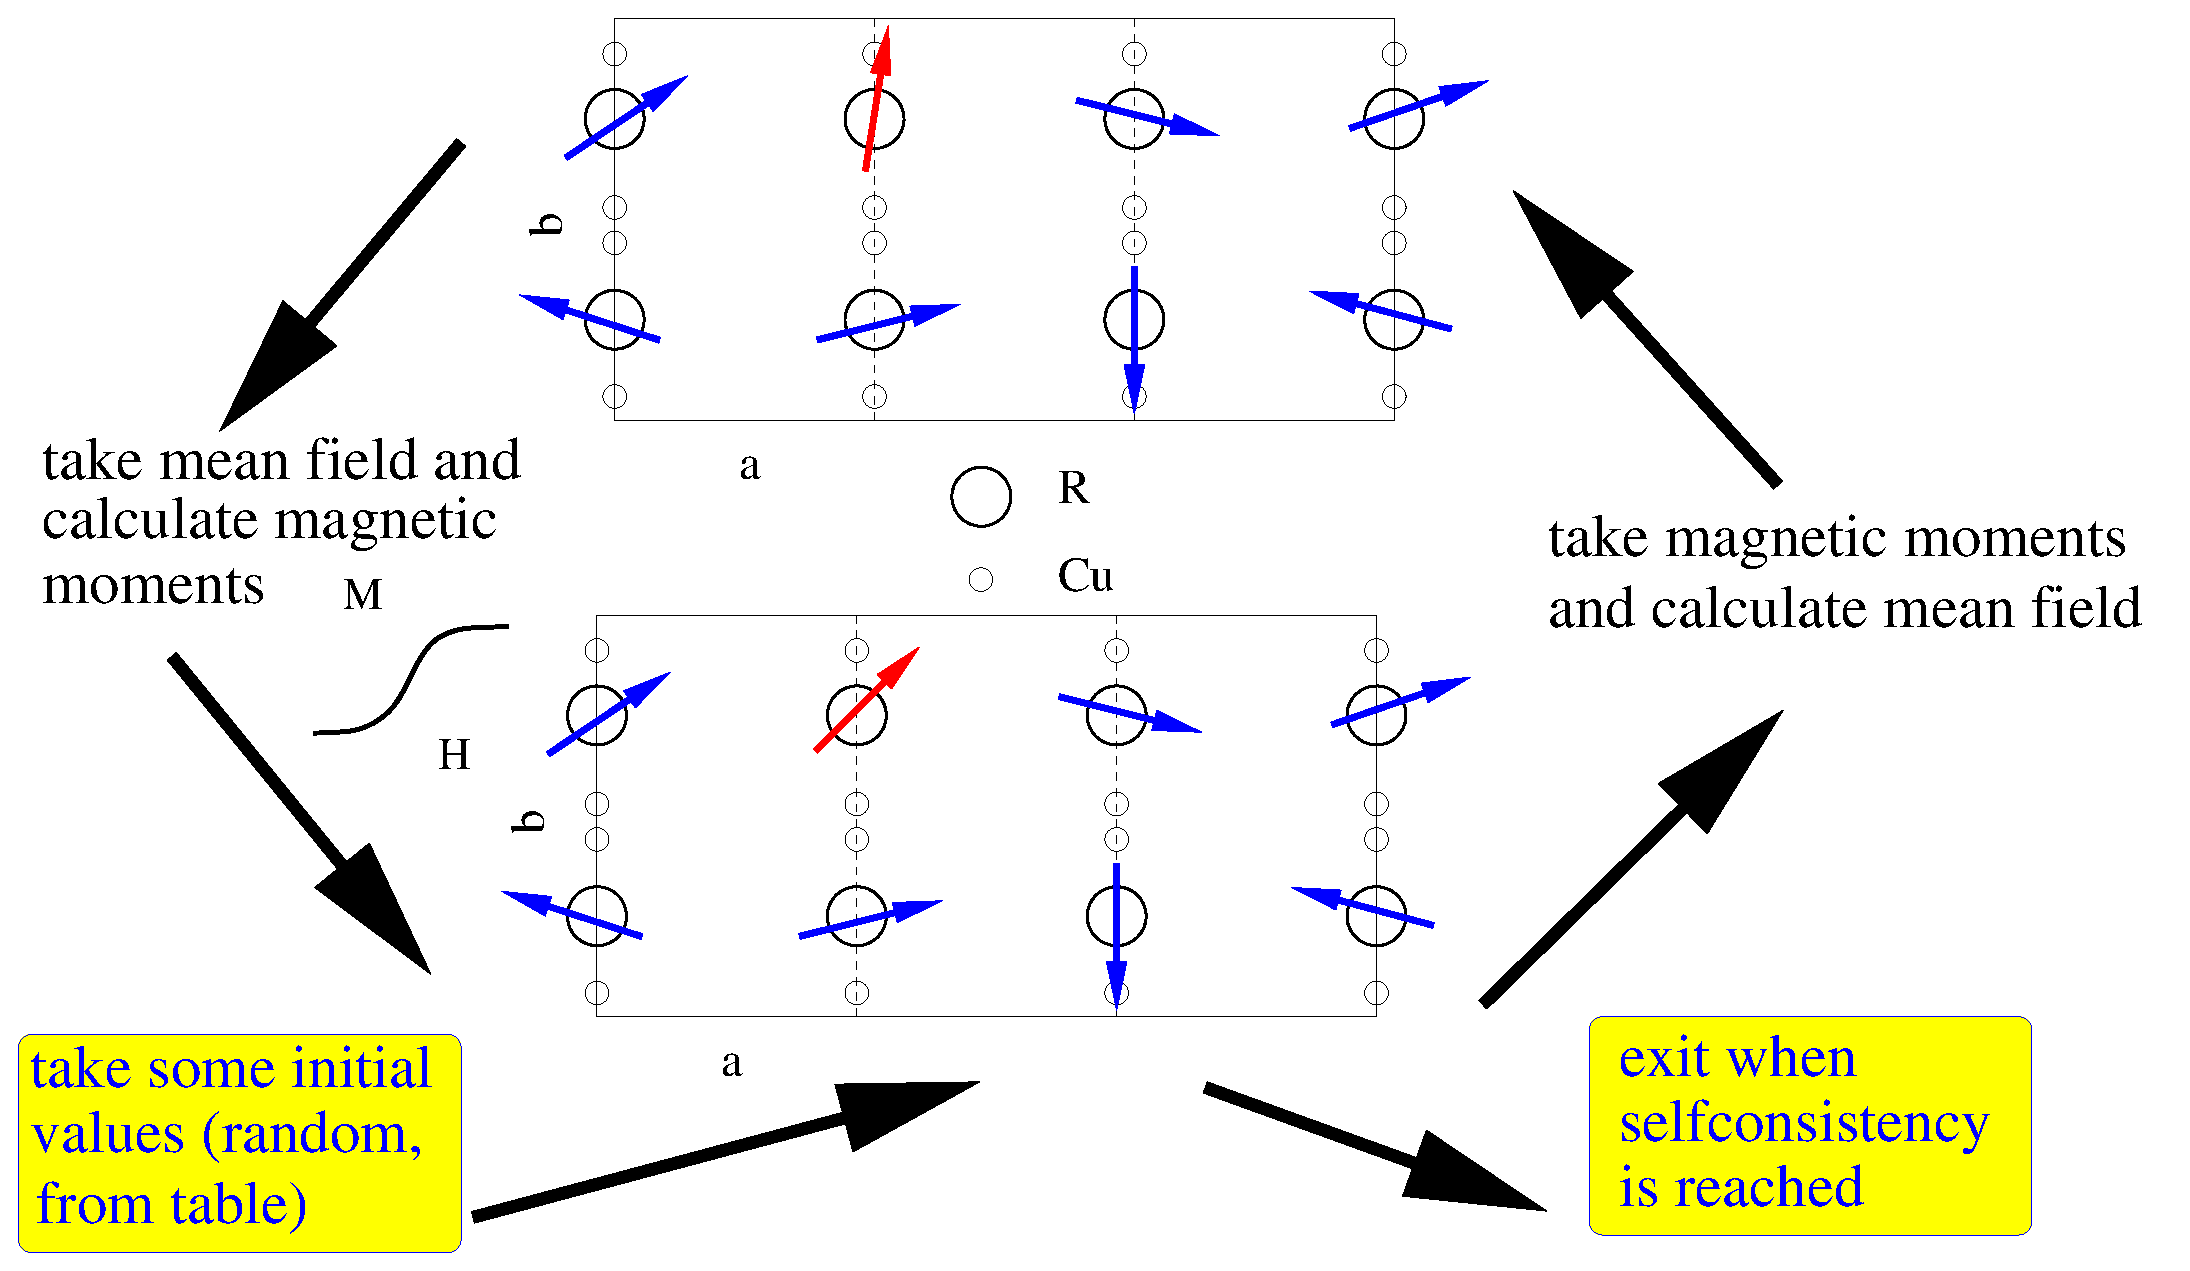
\includegraphics[angle=0,width=0.9\columnwidth]{figsrc/fecalc.eps}
\caption{\label{fecalc}Mean field process of sub {\prg fecalc}.}
\end{figure}

 
\subsubsection{Example {\prg mcphas.ini\index{mcphas.ini}} file for a simple antiferromagnet}

Here is an example of {\prg mcphas.ini\index{mcphas.ini}}, the comments describe the meaning of the different
parameters:

\input{mcphas.ini}



\subsubsection{{\prg mcphas.j\index{mcphas.j}} - lattice and exchange parameters}\label{mcphasj}
This file provides the information about 
the crystallographic
 structure and the magnetic exchange interactions.
For every atom in the crystallographic basis there
has to be given the coordinates, the number of neighbours to be considered, the 
Land\'e factor $g_J$, the single ion property filename and  a set of exchange parameters.
If the exchange parameters (and neighbour positions) are not known for your system, you 
can use the program module {\prg makenn\index{makenn}} (see section \ref{addprog}) to generate 
a list of nearest neighbours and
exchange parameters, currently implemented in {\prg makenn\index{makenn}} are dipolar interactions,
exchange interactions via the Bethe-Slater curve or the RKKY model. Note that in order
to use {\prg makenn\index{makenn}} you have to set up a working {\prg mcphas.j\index{mcphas.j}} file, which may or
may not contain neighbours and interactions.

Use program {\prg addj\index{addj}} to add exchange parameter set stored in different 
such {\prg .j} files (see section~\ref{addprog}).



\begin{description}
\item [Line 1,2:] Comment Lines
\item [Line 3:] lattice constants a,b,c and crystal angles alpha, beta, gamma 
\item [Line 4-6:] primitive lattice vectors
\item [Line 7:] Number of atoms in the primitive crystallographic unit cell ({\prg nofatoms})
\item [Line 8:] a comment line with stars
\item [Line 9:] coordinates  ($d_a$,$d_b$,$d_c$) of 1$^{st}$ magnetic ion in the crystallographic unit cell  with
respect to the lattice vectors $\vec a$,$\vec b$,$\vec c$. The number of neighbours of this 
ion, for which interaction constants are given in the interaction table (nofneighbours). 
If {\prg diagonalexchange}
is set to 0 the 9 components of the exchange tensor are given in column 4-12. 
If {\prg diagonalexchange}
 is 1, only 3 components are given (column 4-6).
If {\prg diagonalexchange}
 is 2, specific components of the exchange tensor can be given in columns 4 onwards. The indices of these components
 must be given in the following line (Line 9a below).
The Land\'e factor of the ion (gJ) and the file name of the corresponding single ion
parameter file (cffilename).
\item [Line 9a:]  If {\prg diagonalexchange=2}, then this line gives the indices of the exchange tensor corresponding to 
 the columns 4 onwards. It must have a variable called {\prg indexexchange} followed by a list of names of components of the interaction
 tensor separated by space. E.g.
 \verb|  #! indexexchange= JaJb JbJc  | 
means column 4 gives the the interaction constant between the
 first angular momentum component of the current ion with the second angular momentum component of its neighbour, whilst 
 column 5 has the interaction constant between the second angular momentum component of this ion with the third component of its
 neighbour. Alternatively, pairs of numbers may be given, as in \verb|  #! indexexchange= 1,2 2,3  |
 Additionally another parameter {\prg symmetricexchange} can be set to 1, where the value in each column is also used 
 for the transposed tensor component. Thus \verb|  #! symmetricexchange=1 indexexchange= JaJb  | is the same as \\
 \verb|  #! indexexchange= JaJb JbJa  | where the 4th and 5th column are the same.
\item [Line 10:]  Comment line
\item [Line 11-(10+nofneighbours):] Interaction table for ion number 1.   
Note: the neighbour coordinates (column 1-3) are given with respect to the lattice vectors
$\vec a$,$\vec b$,$\vec c$. The program then calculates from these values the coordinates
with respect to the primitive lattice $\vec r_1$,~$\vec r_2$,~$\vec r_3$.
($ d_a \vec a + d_b \vec b + d_c \vec c = d_1 \vec r_1 + d_2 \vec r_2 + d_3 \vec r_3$).
Column 4,5,6 \dots contain the components of the interaction tensor $\stackrel{=}{\mathcal J}$. 
Note that in case of non-orthogonal axes the 
components of the moments and the interaction tensor $Ja, Jb, Jc, Jaa, Jbb, Jcc, Jab ...$ 
refer to the orthogonal coordinate system
defined with respect to the nonorthogonal lattice $\vec a,\vec b,\vec c$ as
$Jb||\vec b$, $Jc||(\vec a \times \vec b)$ and $Ja$ perpendicular to $Jb$ and $Jc$.
\item [Line (11+nofneighbours) - end:] for each ion in the unit cell line 8 - (10+nofneighbours)
are repeated.
\end{description}


\vspace{0.5cm}

{\small {\bf Information for experienced users:}
\begin{description}
\item[\prg mcphas.jjj:]
format of exchange parameter file, which only needs a reduced set of exchange
parameters in the input file. Using the program {\prg jjj2j} the file can be transformed
to {\prg mcphas.j\index{mcphas.j}} by adding lines for all the equivalent neighbours. The format definition
of {\prg mcphas.jjj} is the same as {\prg mcphas.j\index{mcphas.j}}, however each line denotes several
equivalent neighbour atoms (instead of only one in {\prg mcphas.j\index{mcphas.j}}) according to the
 following rules:
\begin{itemize}
\item If a nonzero coordinate $d_a$ (or $d_b$,$d_c$) in the interaction table
 corresponds to it's value at the nearest
 lattice point of the primitive lattice,
  additional interactions of the same size
with  neighbours with coordinate $-d_a$ (or $-d_b$,$-d_c$, respectively)
are taken into account. This
holds for each of the three coordinates $d_a$,$d_b$ and $d_c$
 resulting in a maximum
number of 8 equivalent neighbours per line in the interaction table.
\item If the value of $d_a$ (or $d_b$,$d_c$) is zero or differs
from it's value at the nearest lattice point of the primitive lattice, it is 
changed to the value at the nearest lattice point and {\bf no} interaction 
with  neighbours with coordinates $-d_a$ (or $-d_b$,$-d_c$) is
 taken into account. If such
 interaction is needed it may be given in a different line and may
have different magnitude. In this way also crystallographic lattices
with no mirror symmetry may be described.
\end{itemize}
\item[\prg mcphas.coq:]   exchange parameters etc [ in old format]...see examples for details, use {\prg coq2jjj} to 
transform {\prg mcphas.coq} to {\prg mcphas.jjj} format
\end{description}

}


\subsubsection{Example {\prg mcphas.j\index{mcphas.j}} file for a simple antiferromagnet}

Here are example files of a tetragonal antiferromagnet with nearest neighbour interactions, all
files are equivalent:

{\small
\begin{verbatim} 
# simple antiferromagnet 
#<!--mcphase.mcphas.j-->
#***************************************************************
# Lattice Constants (A)
#! a=4.3843 b=4.3843 c=2.4194 alpha=  90 beta=  90 gamma=  90
#! r1a=   1 r2a=   0 r3a=   0
#! r1b=   0 r2b=   1 r3b=   0   primitive lattice vectors [a][b][c]
#! r1c=   0 r2c=   0 r3c=   1
#! nofatoms=1  nofcomponents=3  number of atoms in primitive unit cell/number of components of each spin
# ****************************************************************************
#! da=  0 [a] db=  0 [b] dc=  0 nofneighbours=2 diagonalexchange=0 gJ=0.857143 cffilename=Ce3p.sipf
# da[a] db[b] dc[c] Jaa[meV] Jbb[meV] Jcc[meV] Jab[meV] Jba[meV] Jac[meV] Jca[meV] Jbc[meV] Jcb[meV]
+0	+0	+1	-0.1	-0.1	-0.1   0  0  0  0  0  0
+0	+0	-1	-0.1	-0.1	-0.1   0  0  0  0  0  0
#\end{verbatim}
}

Using diagonalexchange this may be shortened to

{\small
\begin{verbatim} 
# simple antiferromagnet 
#<!--mcphase.mcphas.j-->
#***************************************************************
# Lattice Constants (A)
#! a=4.3843 b=4.3843 c=2.4194 alpha=  90 beta=  90 gamma=  90
#! r1a=   1 r2a=   0 r3a=   0
#! r1b=   0 r2b=   1 r3b=   0   primitive lattice vectors [a][b][c]
#! r1c=   0 r2c=   0 r3c=   1
#! nofatoms=1  nofcomponents=3  number of atoms in primitive unit cell/number of components of each spin
# ****************************************************************************
#! da=  0 [a] db=  0 [b] dc=  0 nofneighbours=2 diagonalexchange=1 gJ=0.857143 cffilename=Ce3p.sipf
# da[a] db[b] dc[c] Jaa[meV] Jbb[meV] Jcc[meV] Jab[meV] Jba[meV] Jac[meV] Jca[meV] Jbc[meV] Jcb[meV]
+0	+0	+1	-0.1	-0.1	-0.1   
+0	+0	-1	-0.1	-0.1	-0.1   
#\end{verbatim}
}

with indexexchange option the sequence of two ion interaction parameters can be changed and
zero parameters may be omitted:

{\small
\begin{verbatim} 
# simple antiferromagnet 
#<!--mcphase.mcphas.j-->
#***************************************************************
# Lattice Constants (A)
#! a=4.3843 b=4.3843 c=2.4194 alpha=  90 beta=  90 gamma=  90
#! r1a=   1 r2a=   0 r3a=   0
#! r1b=   0 r2b=   1 r3b=   0   primitive lattice vectors [a][b][c]
#! r1c=   0 r2c=   0 r3c=   1
#! nofatoms=1  nofcomponents=3  number of atoms in primitive unit cell/number of components of each spin
# ****************************************************************************
#! da=  0 [a] db=  0 [b] dc=  0 nofneighbours=2 diagonalexchange=2 gJ=0.857143 cffilename=Ce3p.sipf
# da[a] db[b] dc[c] Jaa[meV] Jbb[meV] Jcc[meV] Jab[meV] Jba[meV] Jac[meV] Jca[meV] Jbc[meV] Jcb[meV]
#! indexexchange = JaJa JaJc JcJa JbJb JcJc
+0	+0	+1	-0.1 0 0 -0.1	-0.1  
+0	+0	-1	-0.1 0 0 -0.1	-0.1  
#\end{verbatim}
}

{\small
\begin{verbatim} 
# simple antiferromagnet 
#<!--mcphase.mcphas.j-->
#***************************************************************
# Lattice Constants (A)
#! a=4.3843 b=4.3843 c=2.4194 alpha=  90 beta=  90 gamma=  90
#! r1a=   1 r2a=   0 r3a=   0
#! r1b=   0 r2b=   1 r3b=   0   primitive lattice vectors [a][b][c]
#! r1c=   0 r2c=   0 r3c=   1
#! nofatoms=1  nofcomponents=3  number of atoms in primitive unit cell/number of components of each spin
# ****************************************************************************
#! da=  0 [a] db=  0 [b] dc=  0 nofneighbours=2 diagonalexchange=2 gJ=0.857143 cffilename=Ce3p.sipf
# da[a] db[b] dc[c] Jaa[meV] Jbb[meV] Jcc[meV] Jab[meV] Jba[meV] Jac[meV] Jca[meV] Jbc[meV] Jcb[meV]
#! indexexchange = 1,1 1,3, 3,1 2,2 3,3
+0	+0	+1	-0.1 0 0 -0.1	-0.1  
+0	+0	-1	-0.1 0 0 -0.1	-0.1  
#\end{verbatim}
}


using symmetricexchange together with indexexchange will assume that the interaction tensor is symmetic and 
only half of it may be given:

{\small
\begin{verbatim} 
# simple antiferromagnet 
#<!--mcphase.mcphas.j-->
#***************************************************************
# Lattice Constants (A)
#! a=4.3843 b=4.3843 c=2.4194 alpha=  90 beta=  90 gamma=  90
#! r1a=   1 r2a=   0 r3a=   0
#! r1b=   0 r2b=   1 r3b=   0   primitive lattice vectors [a][b][c]
#! r1c=   0 r2c=   0 r3c=   1
#! nofatoms=1  nofcomponents=3  number of atoms in primitive unit cell/number of components of each spin
# ****************************************************************************
#! da=  0 [a] db=  0 [b] dc=  0 nofneighbours=2 diagonalexchange=2 gJ=0.857143 cffilename=Ce3p.sipf
# da[a] db[b] dc[c] Jaa[meV] Jbb[meV] Jcc[meV] Jab[meV] Jba[meV] Jac[meV] Jca[meV] Jbc[meV] Jcb[meV]
#! symmetricexchange=1 indexexchange = JaJa JaJc JbJb JcJc
+0	+0	+1	-0.1 0  -0.1	-0.1  
+0	+0	-1	-0.1 0  -0.1	-0.1  
#\end{verbatim}
}


\subsubsection{Single Ion Property Input Files}\label{sifile}

In order to speed up calculations or treat special problems a large 
variety of single ion modules is available. This includes the
option to load a user written single ion module. Details are 
given in chapter~\ref{simod}.

The first time user of {\prg McPhase} should use the module {\prg so1ion}\index{so1ion} and 
create an appropriate single ion property input file as described in
section \ref{cf1ion}. A good starting point are several examples
given in directory {\prg examples}.


\subsubsection{Example single ion property file  for a simple antiferromagnet}

Here is an example file {\prg mcphas.cf1} describing the anisotropy of a 
simple antiferromagnet with Ce atoms having basal plane anisotropy. Note the
axis convention xyz$||$abc, in case of non-orthogonal axes the convention 
is $y||\vec b$, $z||(\vec a \times \vec b)$ and $x$ perpendicular to $y$ and $z$.


\input{mcphas.cf1}

\subsubsection{{\prg mcphas.tst\index{mcphas.tst}} - input file of test spin-configurations (optional)}
This file is optional and contains
some test momentum configurations to be used for the calculation
             of the free energy. Mind that
\begin{itemize}
\item  in the file header the number of atoms in the primitive
       crystallographic unit cell and the number of components
       of the spin vector have to be given.
\item  at the end of the
 file there must be no empty lines !
\end{itemize}

The momentum - configurations tables always refer to spins sitting on
the primitive lattice ${\mbf r}_i$. If more than one atom is in
the primitive basis, the momentum gets $3n$ components ($n=$ number
of atoms in the crystallographic basis). See {\prg ./examples/ndcu2b\_new/} for
examples of a two atom basis. Units of these tables are that of total 
angular momentum $<J>$.

\subsubsection{Example {\prg mcphas.tst\index{mcphas.tst}} file  for a simple antiferromagnet}

Here is the file {\prg mcphas.tst\index{mcphas.tst}} for the simple antiferromagnet example
describing some spin configurations
to be used as starting values for the mean field process:

\input{mcphas.tst}
Note, in case of non-orthogonal axes the convention 
is $mb||\vec b$, $mc||(\vec a \times \vec b)$ and $ma$ perpendicular to $mb$ and $mc$.

\subsubsection{subdirectory {\prg ./results} - directory where calculated data is stored}

In order to be able to save the results of a calculation the directory {\prg ./results} has to
exist. Mind that all files in this directory will be overwritten without warning. 

\subsubsection{subdirectory {\prg ./fit} - experimental data for fit (optional) } 

In order that {\prg McPhase} can calculate the standard deviation between
 experimental data and the results of the simulation, some experimental data
 can be given in the subdirectory {\prg ./fit}. The filenames and the data-format
 are the same as the output files of {\prg McPhas}, e.g. {\prg mcphas.fum}, {\prg mcphas.hkl}
 etc. {\prg McPhase} looks into the directory {\prg ./fit} and if it finds any
 of these files, the standard deviation is increased correspondingly. 

What measurement data can be used to calculate a standard deviation ?

\begin{description}
\item[{\prg mcphas.fum}] if given in column 11, 12, 13 in {\prg ./fit/mcphas.fum} the
            magnetisation in the $a$, $b$ and $c$ direction is used for calculation
	    of the standard deviation sta. The standard deviation is calculated
	    as ${\rm sta}=\sum_{\rm data points i} ({\mbf m}_i^{calc}-{\mbf m}_i^{meas})^2$.
	    All three components of the magnetic moment have to be given and are used.

\end{description}

Note that the measured data has to be given in those (H-T) points which are 
calculated by mcphas\index{mcphas} in order to be used by the program to increase {\prg sta}.
It is usually most effective to fit only few data points, because a large set
of data points will not improve the quality of the fit and only require a large
amount of calculation time.



\subsection{Starting a simulation}
\label{start}

To start the simulation goto the directory containing the
input files {\prg mcphas.ini, mcphas.j, etc. } and type

\begin{description}
\item[\prg mcphas] to run the program generating stepwise $H-T$ values 
              in a loop given by {\prg mcphas.ini\index{mcphas.ini}} (you can also press the
              symbol in the {\prg McPhase - Explorer} window).
\item[\prg mcphas\index{mcphas} [file]]  to run the program with an input file --   
             {\prg file} contains T ha hb hc values to be calculated 
             if [file] is not given, xmin xmax xstep (xT xHa xHb xHc)
             ymin ymax ystep (yT yHa yHb yHc) is read from file {\prg mcphas.ini\index{mcphas.ini}}
	     and phase diagram is calculated
\item[\prg mcphas\index{mcphas} -h]  to  print help and version of {\prg McPhas}.
\item[\prg mcphas\index{mcphas} -stamax 14]  end mcphas\index{mcphas} if standard deviation exceeds 14.
\item[\prg mcphas\index{mcphas} -a] avoid overwriting output files in results, append new results to existing files
\item[\prg mcphas\index{mcphas} -v]  to  enable verbose mode with lots of messages of {\prg McPhas}. Specifically
the verbose mode enables the following features:
  \begin{itemize}
			          \item more information is printed out, 
			          \item the q-vectors file {\prg ./results/mcphas.qvc} will contain 
				    the explicit spin configurations
			          \item the display\index{display} on screen (ghostview window using 
				     {\prg ./results/.sps.eps}) will be updated not only 
				    when a H-T point has been finished but always 
				    when a structure with smaller free energy 
				    has been stabilised
  \end{itemize}
\item[\prg mcphasit\index{mcphas}] to start mcphase in commandline mode without opening any window
\end{description}

\vspace{1cm}
{\em Exercises:}
\begin{itemize}
\item Look at the input files for {\prg McPhase} given in the directory
{\prg examples/ndcu2b\_new}.  How many atoms are contained in the crystallographic basis ?
\item
Start the simulation by typing the command {\prg mcphas}.
\end{itemize}



\subsection{Options for a running simulation}
... when the program is running, the options in the main window
can be changed. Pressing ''displayall'' displays the current spin-configuration
at each iteration step. Pressing ''log fe vs Q'' appends free energy vs Q
data to {\prg mcphas.log} for every ($T-H$) point.


The file {\prg ./results/.spins.eps} is used to show the information about the currently calculated
spin structure on the screen using the postscript file viewer ghostview.

The file {\prg ./results/.mcphas.fum} contains the information of the magnetisation curve
which is currently calculated. This information is automatically displayed on the screen.


The program {\prg display} (see section \ref{display}) can be used 
for the online display\index{display} of any other
curve(s).


\subsection{Output Files - {\prg mcphas.qvc,phs,sps,mf,fum,j1...,xyt,hkl} }\label{outputfiles}
 (in directory ./results/ after a simulation run) 

\begin{figure}[htb]%h=here, t=top, b=bottom, p=separate figure page
\begin{center}\leavevmode
\includegraphics[angle=0, width=0.3\textwidth]{figsrc/magnetization_ndcu2.ps}
\end{center}
\caption{Calculated magnetisation of NdCu$_2$ for field parallel to the orthorhombic $b$-direction.}
\label{magnetization}
\end{figure}

\begin{figure}[htb]%h=here, t=top, b=bottom, p=separate figure page
\begin{center}\leavevmode
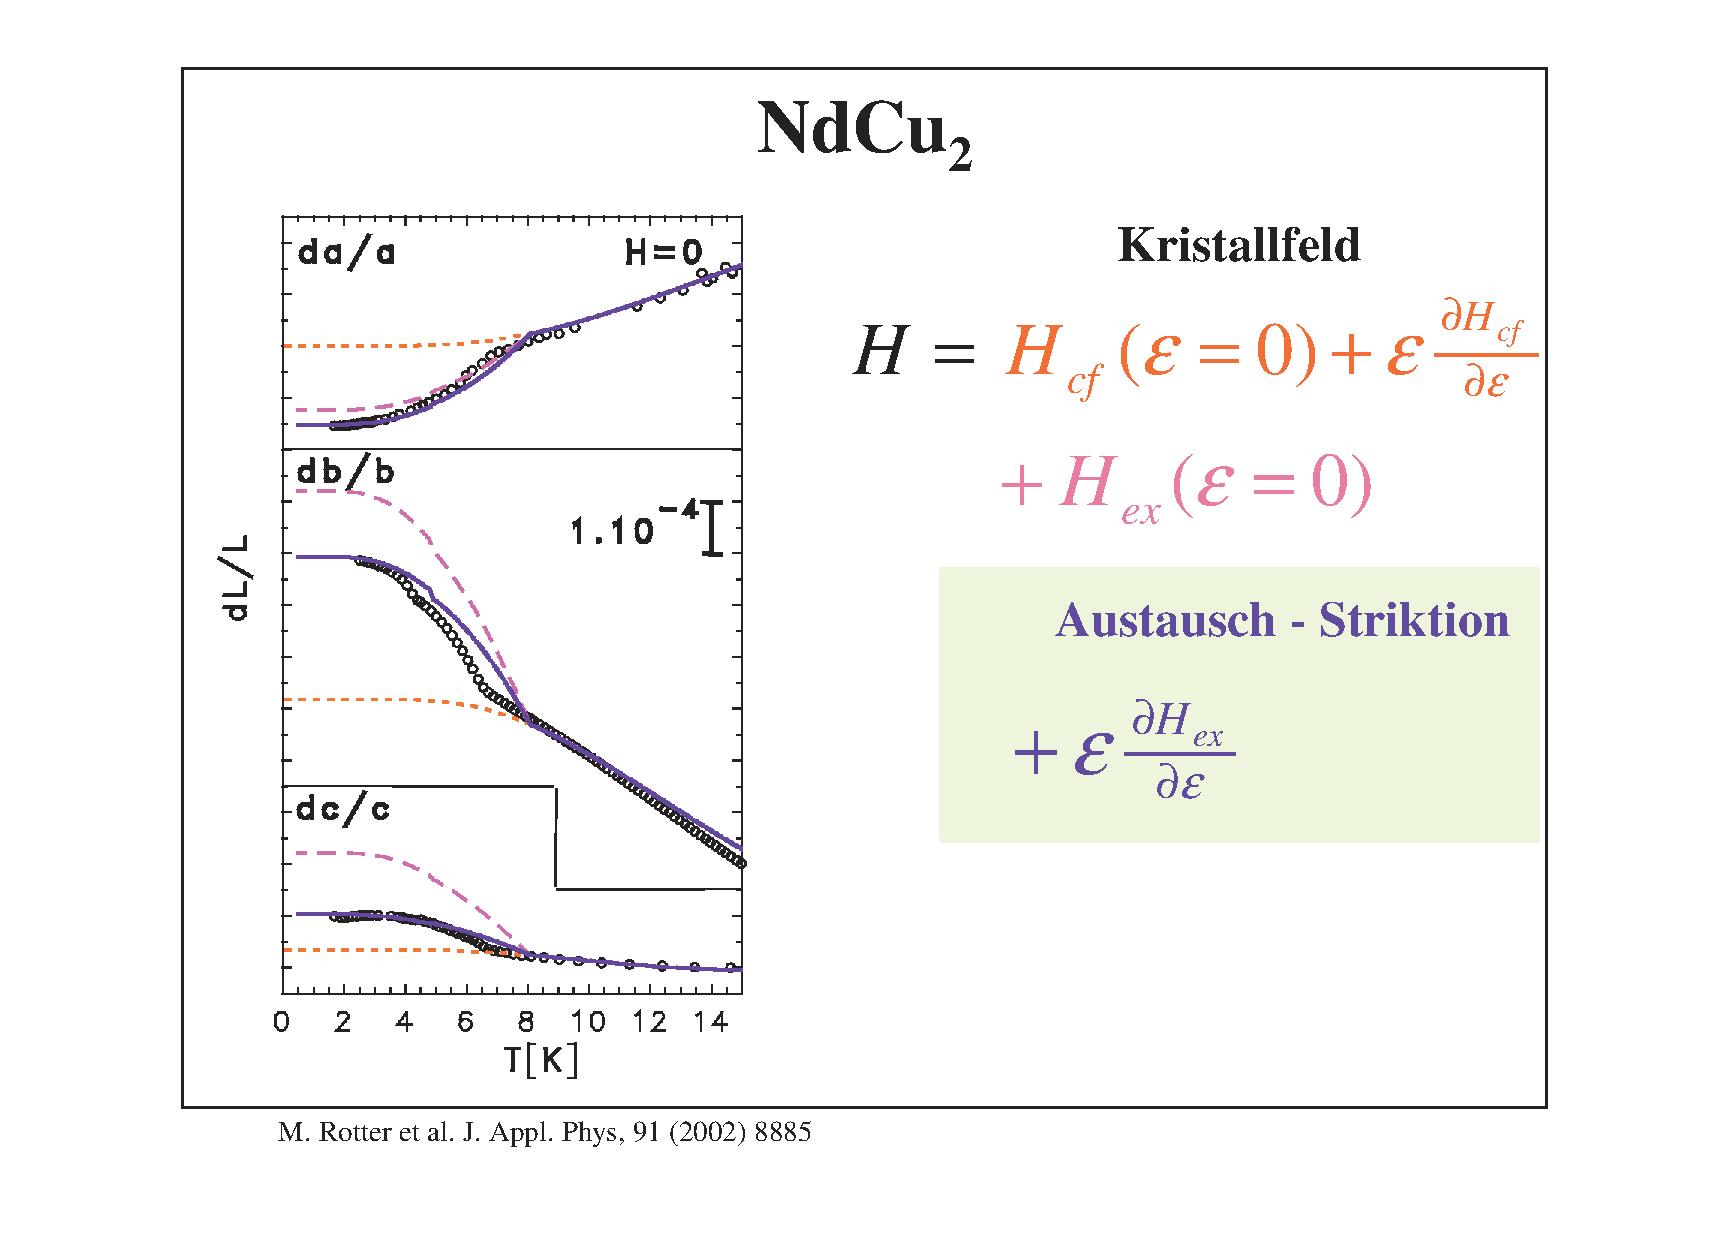
\includegraphics[angle=0, width=0.8\textwidth]{figsrc/magnetostriction_ndcu2.eps}
\end{center}
\caption{Calculated spontaneous magnetostriction of NdCu$_2$.}
\label{magnetostrictiongraphic}
\end{figure}

\begin{description}
\item [\prg mcphas.qvc]    the set of test q-vectors used for calculation of free energy.
                           Components of these q vectors refer to the reciprocal lattice $\vec a^*,\vec b^*,\vec c^*$.
\item [\prg mcphas.phs]    spin-configuration table of different types of spin-configurations. 
                            Note, in case of non-orthogonal axes the convention in these tables 
                            is $mb||\vec b$, $mc||(\vec a \times \vec b)$ and $ma$ perpendicular to $mb$ and $mc$.

                           {\em Note}: 
                           there is no natural criteria for deciding, if one spin-configuration is
			   different from another one. Therefore the list of ''different''
			   spin-configurations is dependent on the meaning of ''different''.
			   
			   The program {\prg McPhase} decides whether a spin-configuration is
			   different from another by a simple criteria, namely by the
			   angle between the spins. Comparing two spin configurations it calculates
			   the angle between corresponding spins and if for one spin the
			   angle is not small, the configuration is treated as a different
			   configuration. Therefore for example a ferromagnet with moments
			   in $a$ has a different spin configuration than a ferromagnet with
			   moments in $b$ direction. 
\item [\prg mcphas.sps]    $T-H$ dependence of spin-configuration. The spin configurations stored in this
                           file may be displayed using the program {\prg spins\index{spins}}, an example is given
			   in figure~\ref{spingraphic}.
                            Note, in case of non-orthogonal axes the convention for applied field $Ha, Hb,Hc$ and
                            also for the moment components $ma, mb, mc$ in these tables 
                            is $mb||\vec b$, $mc||(\vec a \times \vec b)$ and $ma$ perpendicular to $mb$ and $mc$.

\item [\prg mcphas.mf]     $T-H$ dependence of exchange field configuration, stored as $g_J \mu_B H_{xc}(i)$(unit is in meV)
                            for i=1,2,...,number of spins in magnetic unit cell.
                            Note, in case of non-orthogonal axes the convention for applied field $Ha, Hb,Hc$ and
                            also for the mean field components in these tables 
                            is $Hb||\vec b$, $Hc||(\vec a \times \vec b)$ and $Ha$ perpendicular to $Hb$ and $Hc$.
\item [\prg mcphas.fum]    free energy, magnetic energy (the derivative with respect to temperature gives the specific %%@
heat),
                           magnetisation data and (if cfield is used with higher order interactions)
                           expectation values of the Stevens Operators $<O_l^m>$ . As an example for the information
			   contained in this file the calculated magnetisation and magnetostriction of NdCu$_2$ is shown in
			   figures~\ref{magnetization} and ~\ref{magnetizationgraphic}.
                            Note, in case of non-orthogonal axes the convention for applied field $Ha, Hb,Hc$ and
                            also for the magnetisation components $ma,mb,mc$ in these tables 
                            is $Hb||\vec b$, $Hc||(\vec a \times \vec b)$ and $Ha$ perpendicular to $Hb$ and $Hc$.

\item [\prg mcphas1.j1 .j1 .j2 ...] 
               spin-spin correlation functions for sub-lattice 1 neighbour 1 2 ...
	       (linear combination is proportional to magnetostriction)
	       The spin-spin correlation functions for neighbour $k$ are defined by
	       the following sum of dyadic products:

	       \begin{equation}
	        \frac{1}{n}\sum_{s=1}^n <{\mbf J}^s> \times  <{\mbf J}^{s+k}>
	       \end{equation}
	       with $n$ being the number of moments in the magnetic unit cell.
	       Single ion and two-ion magnetostriction can be calculated using the $<O_l^m>$ and the
	       spin-spin correlation functions. As an example the magnetostriction analysis of
	       NdCu$_2$ is shown in figure~\ref{magnetostrictiongraphic}. For details 
             please refer to~\cite{rotter02-8885}.
                            Note, in case of non-orthogonal axes the convention for applied field $Ha, Hb,Hc$ and
                            also for the moment components in these tables 
                            is $Hb||\vec b$, $Hc||(\vec a \times \vec b)$ and $Ha$ perpendicular to $Hb$ and $Hc$.
\item [\prg mcphas.xyt]    phase diagram as x,y,T, H, phase-number j according to spin-configuration table
               given in mcphas.phs, a periodicity key, nettomoments <J>.
 Figure~\ref{phasediagramgraphic}
	       shows the phase diagram of NdCu$_2$ for magnetic fields parallel to the orthorhombic $b$-direction.
                            Note, in case of non-orthogonal axes the convention for applied field $Ha, Hb,Hc$ 
                             in these tables 
                            is $Hb||\vec b$, $Hc||(\vec a \times \vec b)$ and $Ha$ perpendicular to $Hb$ and $Hc$.
\item [\prg mcphas.hkl]    calculated (unpolarised) neutron diffraction data (the calculated magnetic intensities
    correspond to the magnetic structure + Polarisation factor. The
    Lorentz-factor , magnetic form factor and  instrumental corrections are not calculated.)
 As an example figure~\ref{neutintgraphic}
    shows the calculated temperature dependence of magnetic amplitudes for NdCu$_2$.
                           $h,k,l$ refer to the reciprocal lattice $\vec a^*,\vec b^*,\vec c^*$.
                            Note, in case of non-orthogonal axes the convention for applied field $Ha, Hb,Hc$ 
                             in these tables 
                            is $Hb||\vec b$, $Hc||(\vec a \times \vec b)$ and $Ha$ perpendicular to $Hb$ and $Hc$.
    
\item [\prg mcphasa.hkl]    Fourier Transform of the $a$-component of the magnetic Moments.
                           $h,k,l$ refer to the reciprocal lattice $\vec a^*,\vec b^*,\vec c^*$.
                            Note, in case of non-orthogonal axes the convention for applied field $Ha, Hb,Hc$ and
                            the magnetic moment component in these tables 
                            is $Hb||\vec b$, $Hc||(\vec a \times \vec b)$ and $Ha$ perpendicular to $Hb$ and $Hc$.
\item [\prg mcphasb.hkl]    Fourier Transform of the $b$-component of the magnetic Moments.
                           $h,k,l$ refer to the reciprocal lattice $\vec a^*,\vec b^*,\vec c^*$.
                            Note, in case of non-orthogonal axes the convention for applied field $Ha, Hb,Hc$ and
                            the magnetic moment component in these tables 
                            is $Hb||\vec b$, $Hc||(\vec a \times \vec b)$ and $Ha$ perpendicular to $Hb$ and $Hc$.
\item [\prg mcphasc.hkl]    Fourier Transform of the $c$-component of the magnetic Moments.
                           $h,k,l$ refer to the reciprocal lattice $\vec a^*,\vec b^*,\vec c^*$.
                            Note, in case of non-orthogonal axes the convention for applied field $Ha, Hb,Hc$ and
                            the magnetic moment component in these tables 
                            is $Hb||\vec b$, $Hc||(\vec a \times \vec b)$ and $Ha$ perpendicular to $Hb$ and $Hc$.
\end{description} 

\vspace{1cm}
{\em Exercises:}
\begin{itemize}
\item Look at the output files of {\prg McPhase}  in the directory
{\prg examples/ndcu2b\_new/results}.  At which magnetic field
the ferromagnetically aligned state is achieved (at $T=$2~K)?
\item
What is the propagation vector in the different antiferromagnetic phases at $T=$2~K ?
\end{itemize}



\subsubsection{{\prg mcphas.tst\index{mcphas.tst}} - input file of test spin-configurations (optional)}
This file is optional and contains
some test momentum configurations to be used for the calculation
             of the free energy. Mind that
\begin{itemize}
\item  in the file header the number of atoms in the primitive
       crystallographic unit cell and the number of components
       of the spin vector have to be given.
\item  at the end of the
 file there must be no empty lines !
\end{itemize}

The momentum - configurations tables always refer to spins sitting on
the primitive lattice ${\mbf r}_i$. If more than one atom is in
the primitive basis, the momentum gets $3n$ components ($n=$ number
of atoms in the crystallographic basis). See {\prg ./examples/ndcu2b\_new/} for
examples of a two atom basis. Units of these tables are that of total 
angular momentum $<J>$.

\subsubsection{Example {\prg mcphas.tst\index{mcphas.tst}} file  for a simple antiferromagnet}

Here is the file {\prg mcphas.tst\index{mcphas.tst}} for the simple antiferromagnet example
describing some spin configurations
to be used as starting values for the mean field process:

\section{{\prg mcphas} - calculation of thermodynamic properties (Magnetisation, Susceptibility, Specific Heat, Neutron %%@
Diffraction, etc.)}
\label{runmcphas}

In order to perform calculations beyond the capabilities of {\prg cfield\index{cfield}} it is necessary
to use the program {\prg mcphas}. 
\begin{itemize}
\item As a first step it is possible to
calculate the thermodynamic properties such as magnetisation or specific heat
considering only single ion effects. In this case all the exchange parameters
have to be set to zero in {\prg mcphas.j\index{mcphas.j}}. 
\item for more advanced calculations the two - ion interactions have to be
considered and may lead to magnetic order. {\prg mcphas} can perform 
calculations in the ordered state in the following way: for 
a given temperature $T$ and magnetic field $\mbf H$ (vector)
several possible magnetic structures are stabilised
by a mean field algorithm and the free energy is 
calculated. The initial values for this mean-field procedure are
modified by a Monte Carlo process.


The temperature and magnetic field is varied during the calculation
and thereby it is possible to map out the magnetic phase diagram.
\end{itemize}

The program produces a plot of the stabilised magnetic
structures and the magnetisation on screen, the
output files contain additional information 
such as calculated magnetoelastic and  neutron-scattering
data. Several graphic programs easy the visualisation of the
calculated data (section~\ref{graphics}).



\subsection{Input Files}
The program {\prg McPhase} needs the following input files (all in the same directory)
 in order to run:

\begin{enumerate}
\item {\prg mcphas.ini\index{mcphas.ini}}
 - controlling the algorithm
\item {\prg mcphas.j\index{mcphas.j}}
  - lattice and exchange parameters
\item {\prg mcphas.tst\index{mcphas.tst}(optional)}  - test spin configurations
\item {\prg single-ion property files}
\item {\prg directory ./results/}
 - directory where calculated data is stored
\item {\prg directory ./fit} - experimental data for fit (optional)
\end{enumerate}


 All
 of these input files have to be in one directory and the program
has to be started in this directory. The results of the simulation
are then stored in the  subdirectory ./results/, which must exist before starting
the program 
... see directory ./examples/ for some examples.
 In order to prepare these files
for a new calculation it is best to take them from an example, copy the files
to a new directory and make the
modifications  to adapt them to the new problem.

\subsubsection{Example - a simple antiferromagnet}

In the following description of the input files we will always refer
to a simple example: a simple antiferromagnet
on a primitive orthorhombic lattice. The first time user
will thus have a simple example to follow, all corresponding
files are given in the directory {\prg tutorial/03magnetic\_phases\_mcphas/simpleAF}.
 

\subsubsection{{\prg mcphas.ini\index{mcphas.ini}} - controlling the algorithm}
   Initial file containing algorithm control parameters, for instance the range and spacing of
   propagation vectors Q or the number of Monte Carlo trials for initial spin configurations
    - {\em mind}: this
   file is rewritten and reread  when running the program and may be changed by the
   user in order to manipulate the running simulation.

{\prg mcphas.ini\index{mcphas.ini}} consists of several sections:
\begin{description}
\item [MCPHASE RUNTIME CONTROL:] this section contains the parameters
controlling the status of the calculation.
\item [XY PHASEDIAGRAM PARAMETERS:] here the temperature and field range and
step widths of the calculation are specified.
The definition of the x and y
axis in terms of temperature and magnetic field is followed by the
corresponding range and step width. An offset may be given for all
field and temperature values.
Note that for most cases of interest
this offset is zero (T0=0, Ha0=0, Hb0=0, Hc0=0).
 For the simple case of calculating a Temperature-Field phase diagram
 It is just necessary to set xT=1 and give the temperature range by
xmin/xmax/xstep. For field in b direction then just set yHb=1 and 
define the range in ymin/ymax/ystep.
In case of non-orthogonal axes the applied magnetic field
components $Ha, Hb, Hc$ refer to the orthogonal coordinate system
defined with respect to the nonorthogonal lattice $\mbf a,\mbf b,\mbf c$ as
$Hb||\mbf b$, $Hc||(\mbf a \times \mbf b)$ and $Ha$ perpendicular to $Hb$ and $Hc$.

\item [GENERATION OF SPINCONFIGURATIONS:] at the beginning of the program
some initial values of spin configurations are generated from a set of 
propagation vectors. This section defines the range of propagation vectors
and the step width.
Depending on the value of the propagation Q with respect to the primitive reciprocal lattice
1-, 2- or 3-dimensional simulations of magnetic lattices
are possible. It is advisable to 
think carefully about the chosen range and spacing of Q vectors in order
to limit calculation time.
 
For example a good starting point is to begin with a calculation with large
step widths (e.g. 0.1)  covering the Brillouin zone. This should give an idea
of the propagation vectors which are stabilised. An advanced calculation
could then fine tune the propagation and determine its accurate value (using
small step widths in a limited area of the zone).
The verbose option of {\prg mcphas} allows to inspect the propagation vectors
which are actually used in the calculation.
Trick: in order to get a quick overview of the
q-vector range covered by the mcphas\index{mcphas} simulation start mcphas, exit and 
just type {\prg felog ./results/mcphas.qvc} (need {\prg perl,perldl,pdl,pgplot} packages).

In order to limit calculation time, the maximum periodicity
of the magnetic unit cell with respect to the crystallographic unit cell 
(maxqperiod) and the maximum number of spins in the magnetic unit cell 
(maxnofspins) can be limited. Also the maximum number of test spin configurations
in the internal table can be limited (maxnoftestspincf).
A critical feature with respect to calculation time is also the number of
spin configurations which are generated by a random process from a tabulated
SPINCONFIGURATIONS during the calculation. 

In summary the variables in this section are mainly important to adapt the
program to a given computer system with finite speed. They have to be set
to optimise between speed and accuracy of the calculation. In order to
find appropriate values it is best to perform some calculations 
and restrict the parameters step by step if insufficient speed is obtained.
Also the examples included in the program package may serve as starting
points.

\item [PARAMETERS FOR SUB FECALC SELFCONSISTENCY PROCESS:] the most important
procedure in the module {\prg mcphas} is the sub fecalc. In this part of the 
program the self consistent calculation of the magnetic moment configuration
is performed as shown schematically in fig.~\ref{fecalc}. 
In the mean field approximation the Hamiltonian~(\ref{hamilton}) is approximated
by

\begin{equation}
 {\mathcal H}=\sum_n H_{SI}^n + E_{corr}
\end{equation}

with the single ion Hamiltonian (in case of module {\prg so1ion\index{so1ion}})

\begin{equation}
H_{SI}^n=  B_l^m O_{lm}({\mbf J}^n) 
	     - g_{Jn} \mu_B {\mbf J}^n {\mbf H^n_{eff}} 
\end{equation}

and the correction term

\begin{equation}
E_{corr}=\frac{1}{2}\sum_{n} g_{Jn} \mu_B \langle {\mbf J}^n
 \rangle (\mbf H^n_{eff}-\mbf H) 
\end{equation}

and with the mean fields $ \mbf H^n_{eff}$ given by

\begin{equation}\label{meanfield}
\mbf H^n_{eff}=\mbf H + \mbf H^n_{xc}=\mbf H+\sum_{{\mbf G'}n'} \frac{{\mathcal J}
(\mbf r_n-(\mbf G'+\mbf r_{n'}))}{g_{Jn}\mu_B } \langle{\mbf
J}^{n'}\rangle
\end{equation}

These mean fields and the moments $\langle \mbf J^n \rangle$ 
are determined in a self consistent
way. For a given magnetic unit cell and initial configuration 
of magnetic moments
the mean fields are calculated according to equation~(\ref{meanfield}). 
Then, for each
magnetic ion the single ion property module is taken 
and the magnetic moment $\langle \mbf J^n \rangle$ is 
calculated from it's mean field. The mean fields are used again in equation~(\ref{meanfield})
and so on .... until convergence is reached. 
Then, the free energy ($f=-kT\sum_n \ln(z_n) + E_{corr}$ ) 
of the stabilised
configuration is calculated (this is why this sub is called {\prg fecalc}). 
The free energies of a lot of different stabilised configurations have to
be compared in order to find out which configuration has lowest free energy, i.e.
is stable in thermal  equilibrium.

It may happen that this process does
not converge due to bad choice of the initial configuration, therefore a maximum number
of mean field loops has to be given by the user.
The results of a calculation may be significantly influenced by
changing parameters such as the maximum number of iteration loops 
in this section. 
In fact the simulation is always a compromise of calculation time and accuracy: if only
a few initial spin configurations are tried at each (H-T) point, the calculation speed is
fast, however it is possible that the program misses the magnetic structure with the
lowest free energy. The same holds if other critical parameters of the simulation are
restricted too much.
 

\item [OUTPUT OF PHYSICAL PROPERTIES:]
Some options for the output of the calculation can be changed in this section.
\end{description}

\begin{figure}[hb]
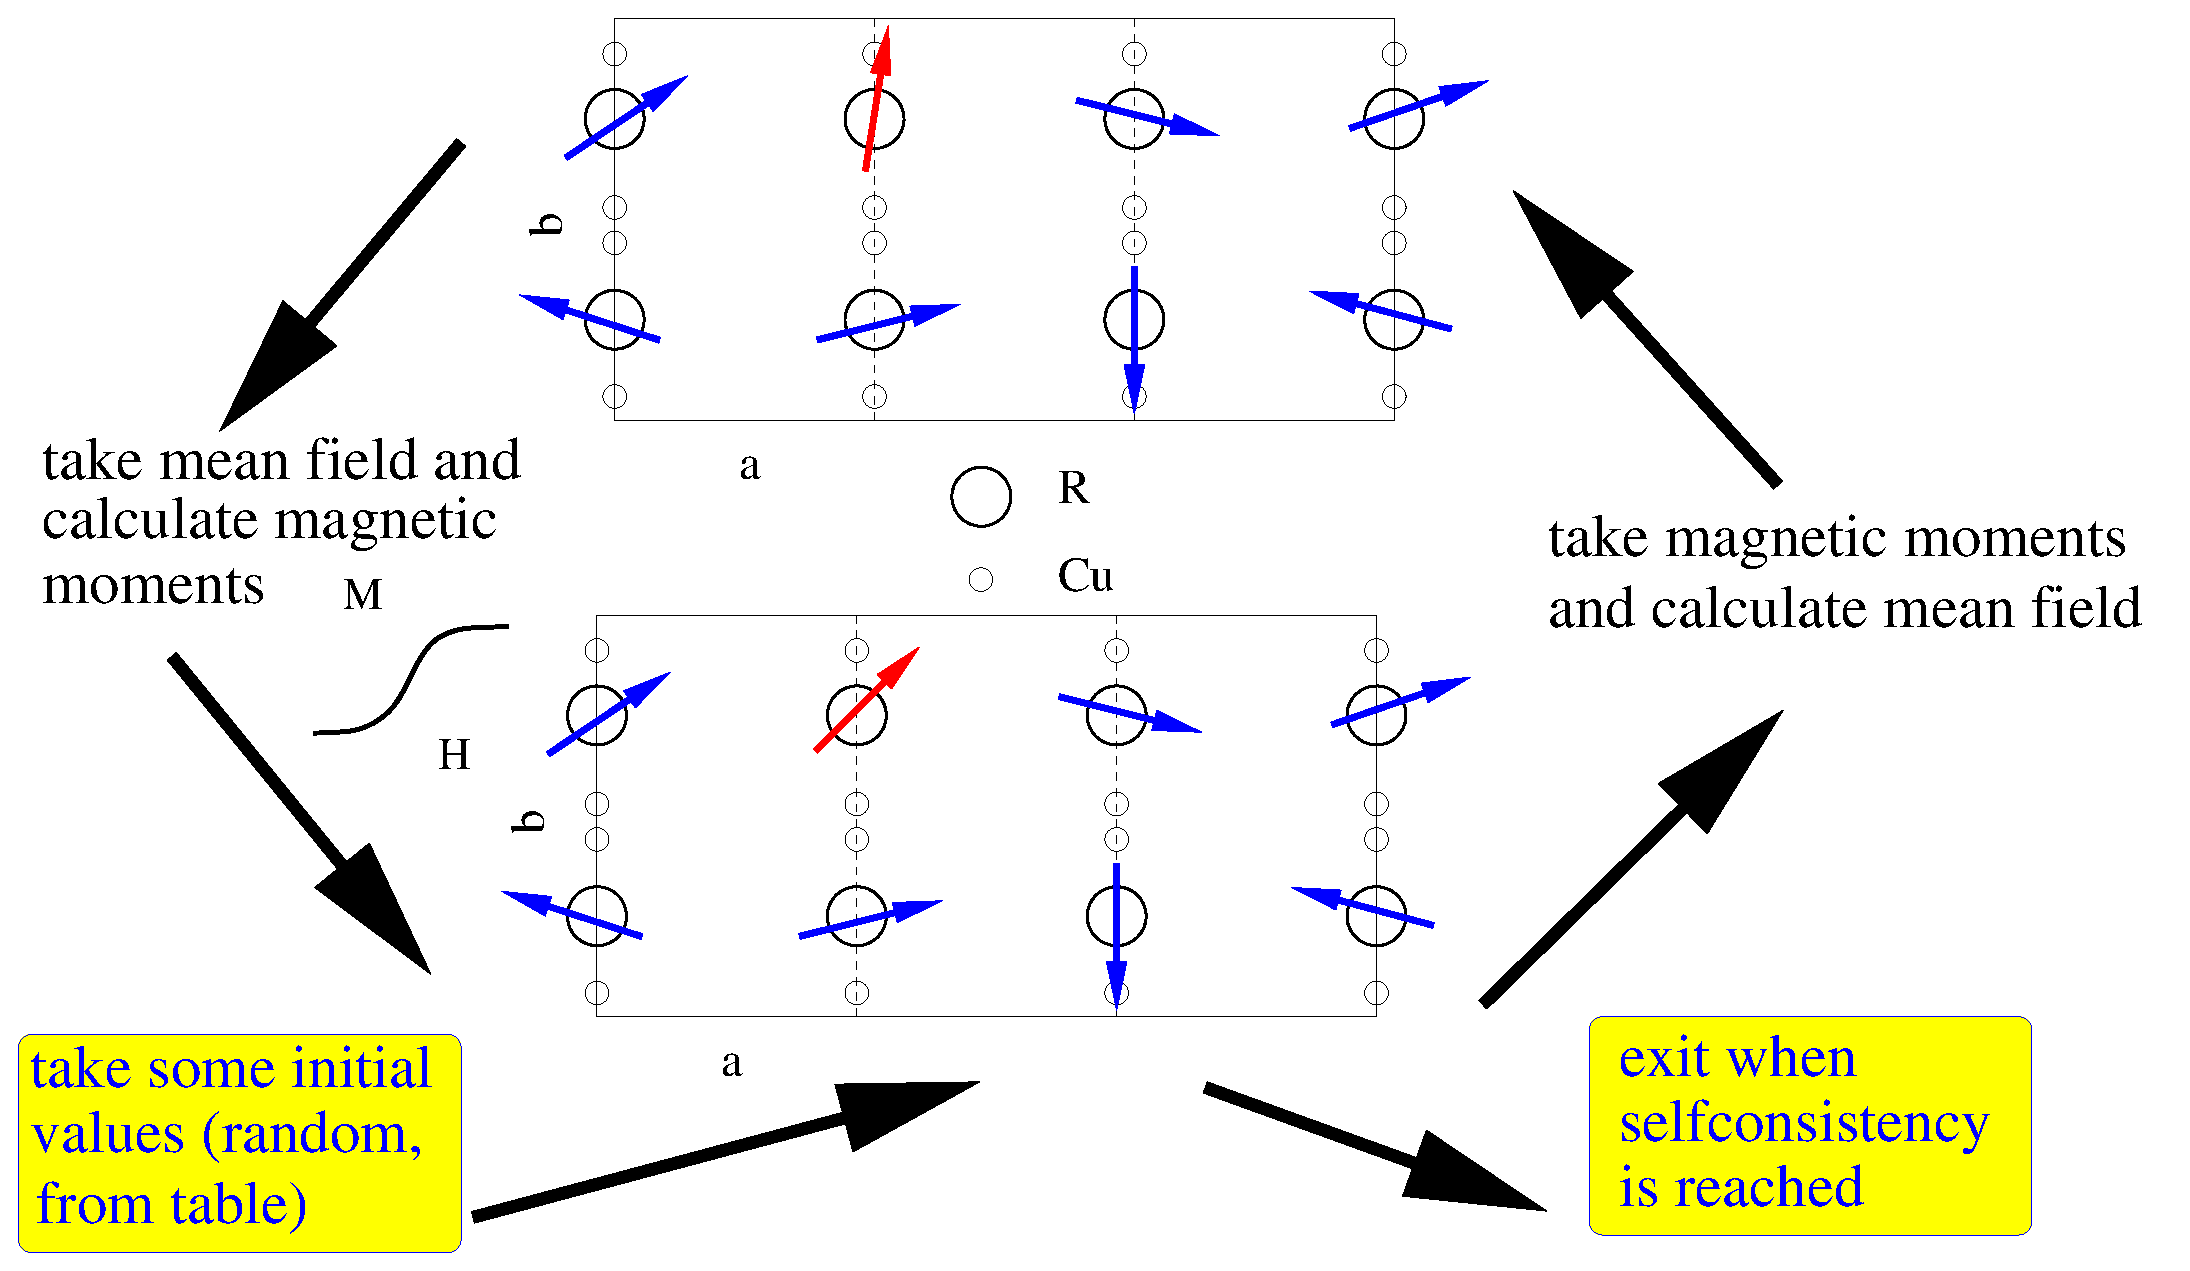
\includegraphics[angle=0,width=0.9\columnwidth]{figsrc/fecalc.eps}
\caption{\label{fecalc}Mean field process of sub {\prg fecalc}.}
\end{figure}

 
\subsubsection{Example {\prg mcphas.ini\index{mcphas.ini}} file for a simple antiferromagnet}

Here is an example of {\prg mcphas.ini\index{mcphas.ini}}, the comments describe the meaning of the different
parameters:

\input{mcphas.ini}



\subsubsection{{\prg mcphas.j\index{mcphas.j}} - lattice and exchange parameters}\label{mcphasj}
This file provides the information about 
the crystallographic
 structure and the magnetic exchange interactions.
For every atom in the crystallographic basis there
has to be given the coordinates, the number of neighbours to be considered, the 
Land\'e factor $g_J$, the single ion property filename and  a set of exchange parameters.
If the exchange parameters (and neighbour positions) are not known for your system, you 
can use the program module {\prg makenn\index{makenn}} (see section \ref{addprog}) to generate 
a list of nearest neighbours and
exchange parameters, currently implemented in {\prg makenn\index{makenn}} are dipolar interactions,
exchange interactions via the Bethe-Slater curve or the RKKY model. Note that in order
to use {\prg makenn\index{makenn}} you have to set up a working {\prg mcphas.j\index{mcphas.j}} file, which may or
may not contain neighbours and interactions.

Use program {\prg addj\index{addj}} to add exchange parameter set stored in different 
such {\prg .j} files (see section~\ref{addprog}).



\begin{description}
\item [Line 1,2:] Comment Lines
\item [Line 3:] lattice constants a,b,c and crystal angles alpha, beta, gamma 
\item [Line 4-6:] primitive lattice vectors
\item [Line 7:] Number of atoms in the primitive crystallographic unit cell ({\prg nofatoms})
\item [Line 8:] a comment line with stars
\item [Line 9:] coordinates  ($d_a$,$d_b$,$d_c$) of 1$^{st}$ magnetic ion in the crystallographic unit cell  with
respect to the lattice vectors $\vec a$,$\vec b$,$\vec c$. The number of neighbours of this 
ion, for which interaction constants are given in the interaction table (nofneighbours). 
If {\prg diagonalexchange}
is set to 0 the 9 components of the exchange tensor are given in column 4-12. 
If {\prg diagonalexchange}
 is 1, only 3 components are given (column 4-6).
If {\prg diagonalexchange}
 is 2, specific components of the exchange tensor can be given in columns 4 onwards. The indices of these components
 must be given in the following line (Line 9a below).
The Land\'e factor of the ion (gJ) and the file name of the corresponding single ion
parameter file (cffilename).
\item [Line 9a:]  If {\prg diagonalexchange=2}, then this line gives the indices of the exchange tensor corresponding to 
 the columns 4 onwards. It must have a variable called {\prg indexexchange} followed by a list of names of components of the interaction
 tensor separated by space. E.g.
 \verb|  #! indexexchange= JaJb JbJc  | 
means column 4 gives the the interaction constant between the
 first angular momentum component of the current ion with the second angular momentum component of its neighbour, whilst 
 column 5 has the interaction constant between the second angular momentum component of this ion with the third component of its
 neighbour. Alternatively, pairs of numbers may be given, as in \verb|  #! indexexchange= 1,2 2,3  |
 Additionally another parameter {\prg symmetricexchange} can be set to 1, where the value in each column is also used 
 for the transposed tensor component. Thus \verb|  #! symmetricexchange=1 indexexchange= JaJb  | is the same as \\
 \verb|  #! indexexchange= JaJb JbJa  | where the 4th and 5th column are the same.
\item [Line 10:]  Comment line
\item [Line 11-(10+nofneighbours):] Interaction table for ion number 1.   
Note: the neighbour coordinates (column 1-3) are given with respect to the lattice vectors
$\vec a$,$\vec b$,$\vec c$. The program then calculates from these values the coordinates
with respect to the primitive lattice $\vec r_1$,~$\vec r_2$,~$\vec r_3$.
($ d_a \vec a + d_b \vec b + d_c \vec c = d_1 \vec r_1 + d_2 \vec r_2 + d_3 \vec r_3$).
Column 4,5,6 \dots contain the components of the interaction tensor $\stackrel{=}{\mathcal J}$. 
Note that in case of non-orthogonal axes the 
components of the moments and the interaction tensor $Ja, Jb, Jc, Jaa, Jbb, Jcc, Jab ...$ 
refer to the orthogonal coordinate system
defined with respect to the nonorthogonal lattice $\vec a,\vec b,\vec c$ as
$Jb||\vec b$, $Jc||(\vec a \times \vec b)$ and $Ja$ perpendicular to $Jb$ and $Jc$.
\item [Line (11+nofneighbours) - end:] for each ion in the unit cell line 8 - (10+nofneighbours)
are repeated.
\end{description}


\vspace{0.5cm}

{\small {\bf Information for experienced users:}
\begin{description}
\item[\prg mcphas.jjj:]
format of exchange parameter file, which only needs a reduced set of exchange
parameters in the input file. Using the program {\prg jjj2j} the file can be transformed
to {\prg mcphas.j\index{mcphas.j}} by adding lines for all the equivalent neighbours. The format definition
of {\prg mcphas.jjj} is the same as {\prg mcphas.j\index{mcphas.j}}, however each line denotes several
equivalent neighbour atoms (instead of only one in {\prg mcphas.j\index{mcphas.j}}) according to the
 following rules:
\begin{itemize}
\item If a nonzero coordinate $d_a$ (or $d_b$,$d_c$) in the interaction table
 corresponds to it's value at the nearest
 lattice point of the primitive lattice,
  additional interactions of the same size
with  neighbours with coordinate $-d_a$ (or $-d_b$,$-d_c$, respectively)
are taken into account. This
holds for each of the three coordinates $d_a$,$d_b$ and $d_c$
 resulting in a maximum
number of 8 equivalent neighbours per line in the interaction table.
\item If the value of $d_a$ (or $d_b$,$d_c$) is zero or differs
from it's value at the nearest lattice point of the primitive lattice, it is 
changed to the value at the nearest lattice point and {\bf no} interaction 
with  neighbours with coordinates $-d_a$ (or $-d_b$,$-d_c$) is
 taken into account. If such
 interaction is needed it may be given in a different line and may
have different magnitude. In this way also crystallographic lattices
with no mirror symmetry may be described.
\end{itemize}
\item[\prg mcphas.coq:]   exchange parameters etc [ in old format]...see examples for details, use {\prg coq2jjj} to 
transform {\prg mcphas.coq} to {\prg mcphas.jjj} format
\end{description}

}


\subsubsection{Example {\prg mcphas.j\index{mcphas.j}} file for a simple antiferromagnet}

Here are example files of a tetragonal antiferromagnet with nearest neighbour interactions, all
files are equivalent:

{\small
\begin{verbatim} 
# simple antiferromagnet 
#<!--mcphase.mcphas.j-->
#***************************************************************
# Lattice Constants (A)
#! a=4.3843 b=4.3843 c=2.4194 alpha=  90 beta=  90 gamma=  90
#! r1a=   1 r2a=   0 r3a=   0
#! r1b=   0 r2b=   1 r3b=   0   primitive lattice vectors [a][b][c]
#! r1c=   0 r2c=   0 r3c=   1
#! nofatoms=1  nofcomponents=3  number of atoms in primitive unit cell/number of components of each spin
# ****************************************************************************
#! da=  0 [a] db=  0 [b] dc=  0 nofneighbours=2 diagonalexchange=0 gJ=0.857143 cffilename=Ce3p.sipf
# da[a] db[b] dc[c] Jaa[meV] Jbb[meV] Jcc[meV] Jab[meV] Jba[meV] Jac[meV] Jca[meV] Jbc[meV] Jcb[meV]
+0	+0	+1	-0.1	-0.1	-0.1   0  0  0  0  0  0
+0	+0	-1	-0.1	-0.1	-0.1   0  0  0  0  0  0
#\end{verbatim}
}

Using diagonalexchange this may be shortened to

{\small
\begin{verbatim} 
# simple antiferromagnet 
#<!--mcphase.mcphas.j-->
#***************************************************************
# Lattice Constants (A)
#! a=4.3843 b=4.3843 c=2.4194 alpha=  90 beta=  90 gamma=  90
#! r1a=   1 r2a=   0 r3a=   0
#! r1b=   0 r2b=   1 r3b=   0   primitive lattice vectors [a][b][c]
#! r1c=   0 r2c=   0 r3c=   1
#! nofatoms=1  nofcomponents=3  number of atoms in primitive unit cell/number of components of each spin
# ****************************************************************************
#! da=  0 [a] db=  0 [b] dc=  0 nofneighbours=2 diagonalexchange=1 gJ=0.857143 cffilename=Ce3p.sipf
# da[a] db[b] dc[c] Jaa[meV] Jbb[meV] Jcc[meV] Jab[meV] Jba[meV] Jac[meV] Jca[meV] Jbc[meV] Jcb[meV]
+0	+0	+1	-0.1	-0.1	-0.1   
+0	+0	-1	-0.1	-0.1	-0.1   
#\end{verbatim}
}

with indexexchange option the sequence of two ion interaction parameters can be changed and
zero parameters may be omitted:

{\small
\begin{verbatim} 
# simple antiferromagnet 
#<!--mcphase.mcphas.j-->
#***************************************************************
# Lattice Constants (A)
#! a=4.3843 b=4.3843 c=2.4194 alpha=  90 beta=  90 gamma=  90
#! r1a=   1 r2a=   0 r3a=   0
#! r1b=   0 r2b=   1 r3b=   0   primitive lattice vectors [a][b][c]
#! r1c=   0 r2c=   0 r3c=   1
#! nofatoms=1  nofcomponents=3  number of atoms in primitive unit cell/number of components of each spin
# ****************************************************************************
#! da=  0 [a] db=  0 [b] dc=  0 nofneighbours=2 diagonalexchange=2 gJ=0.857143 cffilename=Ce3p.sipf
# da[a] db[b] dc[c] Jaa[meV] Jbb[meV] Jcc[meV] Jab[meV] Jba[meV] Jac[meV] Jca[meV] Jbc[meV] Jcb[meV]
#! indexexchange = JaJa JaJc JcJa JbJb JcJc
+0	+0	+1	-0.1 0 0 -0.1	-0.1  
+0	+0	-1	-0.1 0 0 -0.1	-0.1  
#\end{verbatim}
}

{\small
\begin{verbatim} 
# simple antiferromagnet 
#<!--mcphase.mcphas.j-->
#***************************************************************
# Lattice Constants (A)
#! a=4.3843 b=4.3843 c=2.4194 alpha=  90 beta=  90 gamma=  90
#! r1a=   1 r2a=   0 r3a=   0
#! r1b=   0 r2b=   1 r3b=   0   primitive lattice vectors [a][b][c]
#! r1c=   0 r2c=   0 r3c=   1
#! nofatoms=1  nofcomponents=3  number of atoms in primitive unit cell/number of components of each spin
# ****************************************************************************
#! da=  0 [a] db=  0 [b] dc=  0 nofneighbours=2 diagonalexchange=2 gJ=0.857143 cffilename=Ce3p.sipf
# da[a] db[b] dc[c] Jaa[meV] Jbb[meV] Jcc[meV] Jab[meV] Jba[meV] Jac[meV] Jca[meV] Jbc[meV] Jcb[meV]
#! indexexchange = 1,1 1,3, 3,1 2,2 3,3
+0	+0	+1	-0.1 0 0 -0.1	-0.1  
+0	+0	-1	-0.1 0 0 -0.1	-0.1  
#\end{verbatim}
}


using symmetricexchange together with indexexchange will assume that the interaction tensor is symmetic and 
only half of it may be given:

{\small
\begin{verbatim} 
# simple antiferromagnet 
#<!--mcphase.mcphas.j-->
#***************************************************************
# Lattice Constants (A)
#! a=4.3843 b=4.3843 c=2.4194 alpha=  90 beta=  90 gamma=  90
#! r1a=   1 r2a=   0 r3a=   0
#! r1b=   0 r2b=   1 r3b=   0   primitive lattice vectors [a][b][c]
#! r1c=   0 r2c=   0 r3c=   1
#! nofatoms=1  nofcomponents=3  number of atoms in primitive unit cell/number of components of each spin
# ****************************************************************************
#! da=  0 [a] db=  0 [b] dc=  0 nofneighbours=2 diagonalexchange=2 gJ=0.857143 cffilename=Ce3p.sipf
# da[a] db[b] dc[c] Jaa[meV] Jbb[meV] Jcc[meV] Jab[meV] Jba[meV] Jac[meV] Jca[meV] Jbc[meV] Jcb[meV]
#! symmetricexchange=1 indexexchange = JaJa JaJc JbJb JcJc
+0	+0	+1	-0.1 0  -0.1	-0.1  
+0	+0	-1	-0.1 0  -0.1	-0.1  
#\end{verbatim}
}


\subsubsection{Single Ion Property Input Files}\label{sifile}

In order to speed up calculations or treat special problems a large 
variety of single ion modules is available. This includes the
option to load a user written single ion module. Details are 
given in chapter~\ref{simod}.

The first time user of {\prg McPhase} should use the module {\prg so1ion}\index{so1ion} and 
create an appropriate single ion property input file as described in
section \ref{cf1ion}. A good starting point are several examples
given in directory {\prg examples}.


\subsubsection{Example single ion property file  for a simple antiferromagnet}

Here is an example file {\prg mcphas.cf1} describing the anisotropy of a 
simple antiferromagnet with Ce atoms having basal plane anisotropy. Note the
axis convention xyz$||$abc, in case of non-orthogonal axes the convention 
is $y||\vec b$, $z||(\vec a \times \vec b)$ and $x$ perpendicular to $y$ and $z$.


\input{mcphas.cf1}

\subsubsection{{\prg mcphas.tst\index{mcphas.tst}} - input file of test spin-configurations (optional)}
This file is optional and contains
some test momentum configurations to be used for the calculation
             of the free energy. Mind that
\begin{itemize}
\item  in the file header the number of atoms in the primitive
       crystallographic unit cell and the number of components
       of the spin vector have to be given.
\item  at the end of the
 file there must be no empty lines !
\end{itemize}

The momentum - configurations tables always refer to spins sitting on
the primitive lattice ${\mbf r}_i$. If more than one atom is in
the primitive basis, the momentum gets $3n$ components ($n=$ number
of atoms in the crystallographic basis). See {\prg ./examples/ndcu2b\_new/} for
examples of a two atom basis. Units of these tables are that of total 
angular momentum $<J>$.

\subsubsection{Example {\prg mcphas.tst\index{mcphas.tst}} file  for a simple antiferromagnet}

Here is the file {\prg mcphas.tst\index{mcphas.tst}} for the simple antiferromagnet example
describing some spin configurations
to be used as starting values for the mean field process:

\input{mcphas.tst}
Note, in case of non-orthogonal axes the convention 
is $mb||\vec b$, $mc||(\vec a \times \vec b)$ and $ma$ perpendicular to $mb$ and $mc$.

\subsubsection{subdirectory {\prg ./results} - directory where calculated data is stored}

In order to be able to save the results of a calculation the directory {\prg ./results} has to
exist. Mind that all files in this directory will be overwritten without warning. 

\subsubsection{subdirectory {\prg ./fit} - experimental data for fit (optional) } 

In order that {\prg McPhase} can calculate the standard deviation between
 experimental data and the results of the simulation, some experimental data
 can be given in the subdirectory {\prg ./fit}. The filenames and the data-format
 are the same as the output files of {\prg McPhas}, e.g. {\prg mcphas.fum}, {\prg mcphas.hkl}
 etc. {\prg McPhase} looks into the directory {\prg ./fit} and if it finds any
 of these files, the standard deviation is increased correspondingly. 

What measurement data can be used to calculate a standard deviation ?

\begin{description}
\item[{\prg mcphas.fum}] if given in column 11, 12, 13 in {\prg ./fit/mcphas.fum} the
            magnetisation in the $a$, $b$ and $c$ direction is used for calculation
	    of the standard deviation sta. The standard deviation is calculated
	    as ${\rm sta}=\sum_{\rm data points i} ({\mbf m}_i^{calc}-{\mbf m}_i^{meas})^2$.
	    All three components of the magnetic moment have to be given and are used.

\end{description}

Note that the measured data has to be given in those (H-T) points which are 
calculated by mcphas\index{mcphas} in order to be used by the program to increase {\prg sta}.
It is usually most effective to fit only few data points, because a large set
of data points will not improve the quality of the fit and only require a large
amount of calculation time.



\subsection{Starting a simulation}
\label{start}

To start the simulation goto the directory containing the
input files {\prg mcphas.ini, mcphas.j, etc. } and type

\begin{description}
\item[\prg mcphas] to run the program generating stepwise $H-T$ values 
              in a loop given by {\prg mcphas.ini\index{mcphas.ini}} (you can also press the
              symbol in the {\prg McPhase - Explorer} window).
\item[\prg mcphas\index{mcphas} [file]]  to run the program with an input file --   
             {\prg file} contains T ha hb hc values to be calculated 
             if [file] is not given, xmin xmax xstep (xT xHa xHb xHc)
             ymin ymax ystep (yT yHa yHb yHc) is read from file {\prg mcphas.ini\index{mcphas.ini}}
	     and phase diagram is calculated
\item[\prg mcphas\index{mcphas} -h]  to  print help and version of {\prg McPhas}.
\item[\prg mcphas\index{mcphas} -stamax 14]  end mcphas\index{mcphas} if standard deviation exceeds 14.
\item[\prg mcphas\index{mcphas} -a] avoid overwriting output files in results, append new results to existing files
\item[\prg mcphas\index{mcphas} -v]  to  enable verbose mode with lots of messages of {\prg McPhas}. Specifically
the verbose mode enables the following features:
  \begin{itemize}
			          \item more information is printed out, 
			          \item the q-vectors file {\prg ./results/mcphas.qvc} will contain 
				    the explicit spin configurations
			          \item the display\index{display} on screen (ghostview window using 
				     {\prg ./results/.sps.eps}) will be updated not only 
				    when a H-T point has been finished but always 
				    when a structure with smaller free energy 
				    has been stabilised
  \end{itemize}
\item[\prg mcphasit\index{mcphas}] to start mcphase in commandline mode without opening any window
\end{description}

\vspace{1cm}
{\em Exercises:}
\begin{itemize}
\item Look at the input files for {\prg McPhase} given in the directory
{\prg examples/ndcu2b\_new}.  How many atoms are contained in the crystallographic basis ?
\item
Start the simulation by typing the command {\prg mcphas}.
\end{itemize}



\subsection{Options for a running simulation}
... when the program is running, the options in the main window
can be changed. Pressing ''displayall'' displays the current spin-configuration
at each iteration step. Pressing ''log fe vs Q'' appends free energy vs Q
data to {\prg mcphas.log} for every ($T-H$) point.


The file {\prg ./results/.spins.eps} is used to show the information about the currently calculated
spin structure on the screen using the postscript file viewer ghostview.

The file {\prg ./results/.mcphas.fum} contains the information of the magnetisation curve
which is currently calculated. This information is automatically displayed on the screen.


The program {\prg display} (see section \ref{display}) can be used 
for the online display\index{display} of any other
curve(s).


\subsection{Output Files - {\prg mcphas.qvc,phs,sps,mf,fum,j1...,xyt,hkl} }\label{outputfiles}
 (in directory ./results/ after a simulation run) 

\begin{figure}[htb]%h=here, t=top, b=bottom, p=separate figure page
\begin{center}\leavevmode
\includegraphics[angle=0, width=0.3\textwidth]{figsrc/magnetization_ndcu2.ps}
\end{center}
\caption{Calculated magnetisation of NdCu$_2$ for field parallel to the orthorhombic $b$-direction.}
\label{magnetization}
\end{figure}

\begin{figure}[htb]%h=here, t=top, b=bottom, p=separate figure page
\begin{center}\leavevmode
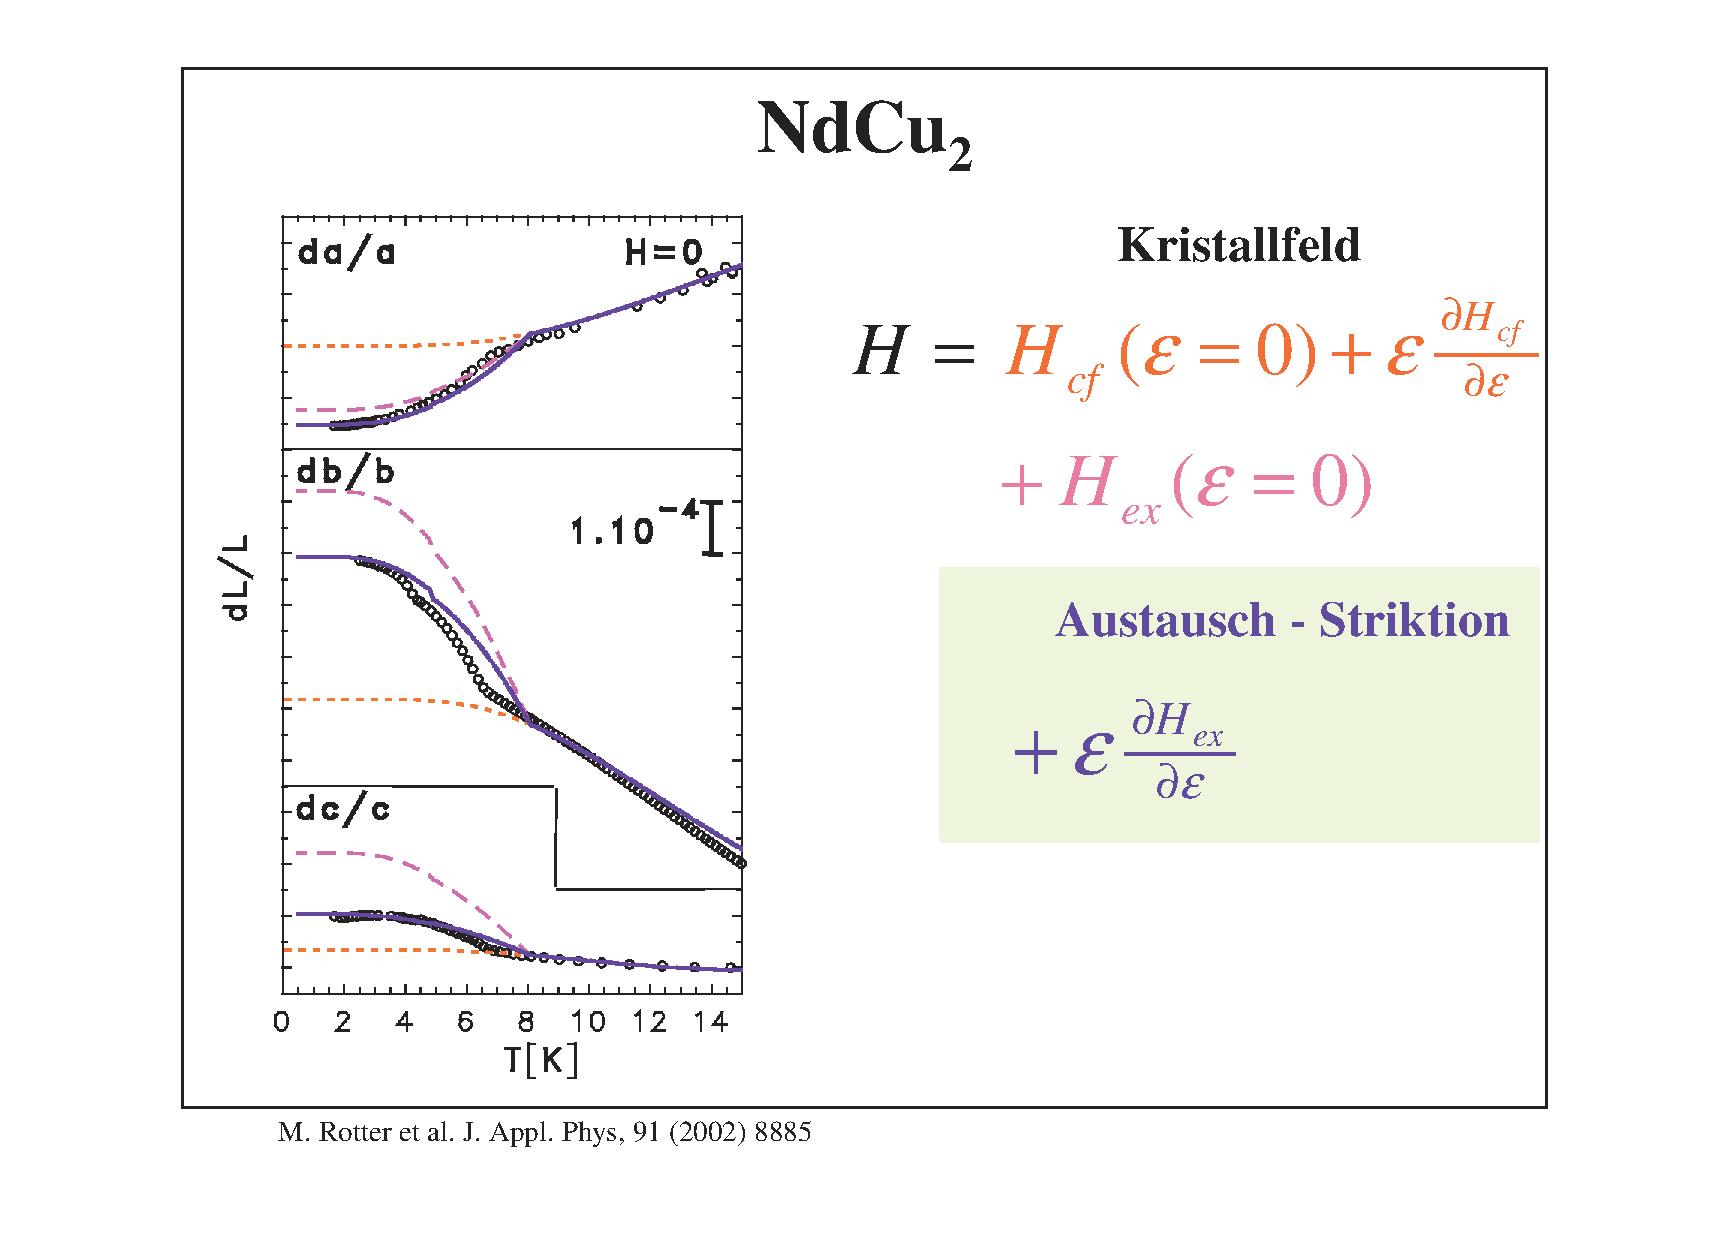
\includegraphics[angle=0, width=0.8\textwidth]{figsrc/magnetostriction_ndcu2.eps}
\end{center}
\caption{Calculated spontaneous magnetostriction of NdCu$_2$.}
\label{magnetostrictiongraphic}
\end{figure}

\begin{description}
\item [\prg mcphas.qvc]    the set of test q-vectors used for calculation of free energy.
                           Components of these q vectors refer to the reciprocal lattice $\vec a^*,\vec b^*,\vec c^*$.
\item [\prg mcphas.phs]    spin-configuration table of different types of spin-configurations. 
                            Note, in case of non-orthogonal axes the convention in these tables 
                            is $mb||\vec b$, $mc||(\vec a \times \vec b)$ and $ma$ perpendicular to $mb$ and $mc$.

                           {\em Note}: 
                           there is no natural criteria for deciding, if one spin-configuration is
			   different from another one. Therefore the list of ''different''
			   spin-configurations is dependent on the meaning of ''different''.
			   
			   The program {\prg McPhase} decides whether a spin-configuration is
			   different from another by a simple criteria, namely by the
			   angle between the spins. Comparing two spin configurations it calculates
			   the angle between corresponding spins and if for one spin the
			   angle is not small, the configuration is treated as a different
			   configuration. Therefore for example a ferromagnet with moments
			   in $a$ has a different spin configuration than a ferromagnet with
			   moments in $b$ direction. 
\item [\prg mcphas.sps]    $T-H$ dependence of spin-configuration. The spin configurations stored in this
                           file may be displayed using the program {\prg spins\index{spins}}, an example is given
			   in figure~\ref{spingraphic}.
                            Note, in case of non-orthogonal axes the convention for applied field $Ha, Hb,Hc$ and
                            also for the moment components $ma, mb, mc$ in these tables 
                            is $mb||\vec b$, $mc||(\vec a \times \vec b)$ and $ma$ perpendicular to $mb$ and $mc$.

\item [\prg mcphas.mf]     $T-H$ dependence of exchange field configuration, stored as $g_J \mu_B H_{xc}(i)$(unit is in meV)
                            for i=1,2,...,number of spins in magnetic unit cell.
                            Note, in case of non-orthogonal axes the convention for applied field $Ha, Hb,Hc$ and
                            also for the mean field components in these tables 
                            is $Hb||\vec b$, $Hc||(\vec a \times \vec b)$ and $Ha$ perpendicular to $Hb$ and $Hc$.
\item [\prg mcphas.fum]    free energy, magnetic energy (the derivative with respect to temperature gives the specific %%@
heat),
                           magnetisation data and (if cfield is used with higher order interactions)
                           expectation values of the Stevens Operators $<O_l^m>$ . As an example for the information
			   contained in this file the calculated magnetisation and magnetostriction of NdCu$_2$ is shown in
			   figures~\ref{magnetization} and ~\ref{magnetizationgraphic}.
                            Note, in case of non-orthogonal axes the convention for applied field $Ha, Hb,Hc$ and
                            also for the magnetisation components $ma,mb,mc$ in these tables 
                            is $Hb||\vec b$, $Hc||(\vec a \times \vec b)$ and $Ha$ perpendicular to $Hb$ and $Hc$.

\item [\prg mcphas1.j1 .j1 .j2 ...] 
               spin-spin correlation functions for sub-lattice 1 neighbour 1 2 ...
	       (linear combination is proportional to magnetostriction)
	       The spin-spin correlation functions for neighbour $k$ are defined by
	       the following sum of dyadic products:

	       \begin{equation}
	        \frac{1}{n}\sum_{s=1}^n <{\mbf J}^s> \times  <{\mbf J}^{s+k}>
	       \end{equation}
	       with $n$ being the number of moments in the magnetic unit cell.
	       Single ion and two-ion magnetostriction can be calculated using the $<O_l^m>$ and the
	       spin-spin correlation functions. As an example the magnetostriction analysis of
	       NdCu$_2$ is shown in figure~\ref{magnetostrictiongraphic}. For details 
             please refer to~\cite{rotter02-8885}.
                            Note, in case of non-orthogonal axes the convention for applied field $Ha, Hb,Hc$ and
                            also for the moment components in these tables 
                            is $Hb||\vec b$, $Hc||(\vec a \times \vec b)$ and $Ha$ perpendicular to $Hb$ and $Hc$.
\item [\prg mcphas.xyt]    phase diagram as x,y,T, H, phase-number j according to spin-configuration table
               given in mcphas.phs, a periodicity key, nettomoments <J>.
 Figure~\ref{phasediagramgraphic}
	       shows the phase diagram of NdCu$_2$ for magnetic fields parallel to the orthorhombic $b$-direction.
                            Note, in case of non-orthogonal axes the convention for applied field $Ha, Hb,Hc$ 
                             in these tables 
                            is $Hb||\vec b$, $Hc||(\vec a \times \vec b)$ and $Ha$ perpendicular to $Hb$ and $Hc$.
\item [\prg mcphas.hkl]    calculated (unpolarised) neutron diffraction data (the calculated magnetic intensities
    correspond to the magnetic structure + Polarisation factor. The
    Lorentz-factor , magnetic form factor and  instrumental corrections are not calculated.)
 As an example figure~\ref{neutintgraphic}
    shows the calculated temperature dependence of magnetic amplitudes for NdCu$_2$.
                           $h,k,l$ refer to the reciprocal lattice $\vec a^*,\vec b^*,\vec c^*$.
                            Note, in case of non-orthogonal axes the convention for applied field $Ha, Hb,Hc$ 
                             in these tables 
                            is $Hb||\vec b$, $Hc||(\vec a \times \vec b)$ and $Ha$ perpendicular to $Hb$ and $Hc$.
    
\item [\prg mcphasa.hkl]    Fourier Transform of the $a$-component of the magnetic Moments.
                           $h,k,l$ refer to the reciprocal lattice $\vec a^*,\vec b^*,\vec c^*$.
                            Note, in case of non-orthogonal axes the convention for applied field $Ha, Hb,Hc$ and
                            the magnetic moment component in these tables 
                            is $Hb||\vec b$, $Hc||(\vec a \times \vec b)$ and $Ha$ perpendicular to $Hb$ and $Hc$.
\item [\prg mcphasb.hkl]    Fourier Transform of the $b$-component of the magnetic Moments.
                           $h,k,l$ refer to the reciprocal lattice $\vec a^*,\vec b^*,\vec c^*$.
                            Note, in case of non-orthogonal axes the convention for applied field $Ha, Hb,Hc$ and
                            the magnetic moment component in these tables 
                            is $Hb||\vec b$, $Hc||(\vec a \times \vec b)$ and $Ha$ perpendicular to $Hb$ and $Hc$.
\item [\prg mcphasc.hkl]    Fourier Transform of the $c$-component of the magnetic Moments.
                           $h,k,l$ refer to the reciprocal lattice $\vec a^*,\vec b^*,\vec c^*$.
                            Note, in case of non-orthogonal axes the convention for applied field $Ha, Hb,Hc$ and
                            the magnetic moment component in these tables 
                            is $Hb||\vec b$, $Hc||(\vec a \times \vec b)$ and $Ha$ perpendicular to $Hb$ and $Hc$.
\end{description} 

\vspace{1cm}
{\em Exercises:}
\begin{itemize}
\item Look at the output files of {\prg McPhase}  in the directory
{\prg examples/ndcu2b\_new/results}.  At which magnetic field
the ferromagnetically aligned state is achieved (at $T=$2~K)?
\item
What is the propagation vector in the different antiferromagnetic phases at $T=$2~K ?
\end{itemize}


Note, in case of non-orthogonal axes the convention 
is $mb||\vec b$, $mc||(\vec a \times \vec b)$ and $ma$ perpendicular to $mb$ and $mc$.

\subsubsection{subdirectory {\prg ./results} - directory where calculated data is stored}

In order to be able to save the results of a calculation the directory {\prg ./results} has to
exist. Mind that all files in this directory will be overwritten without warning. 

\subsubsection{subdirectory {\prg ./fit} - experimental data for fit (optional) } 

In order that {\prg McPhase} can calculate the standard deviation between
 experimental data and the results of the simulation, some experimental data
 can be given in the subdirectory {\prg ./fit}. The filenames and the data-format
 are the same as the output files of {\prg McPhas}, e.g. {\prg mcphas.fum}, {\prg mcphas.hkl}
 etc. {\prg McPhase} looks into the directory {\prg ./fit} and if it finds any
 of these files, the standard deviation is increased correspondingly. 

What measurement data can be used to calculate a standard deviation ?

\begin{description}
\item[{\prg mcphas.fum}] if given in column 11, 12, 13 in {\prg ./fit/mcphas.fum} the
            magnetisation in the $a$, $b$ and $c$ direction is used for calculation
	    of the standard deviation sta. The standard deviation is calculated
	    as ${\rm sta}=\sum_{\rm data points i} ({\mbf m}_i^{calc}-{\mbf m}_i^{meas})^2$.
	    All three components of the magnetic moment have to be given and are used.

\end{description}

Note that the measured data has to be given in those (H-T) points which are 
calculated by mcphas\index{mcphas} in order to be used by the program to increase {\prg sta}.
It is usually most effective to fit only few data points, because a large set
of data points will not improve the quality of the fit and only require a large
amount of calculation time.



\subsection{Starting a simulation}
\label{start}

To start the simulation goto the directory containing the
input files {\prg mcphas.ini, mcphas.j, etc. } and type

\begin{description}
\item[\prg mcphas] to run the program generating stepwise $H-T$ values 
              in a loop given by {\prg mcphas.ini\index{mcphas.ini}} (you can also press the
              symbol in the {\prg McPhase - Explorer} window).
\item[\prg mcphas\index{mcphas} [file]]  to run the program with an input file --   
             {\prg file} contains T ha hb hc values to be calculated 
             if [file] is not given, xmin xmax xstep (xT xHa xHb xHc)
             ymin ymax ystep (yT yHa yHb yHc) is read from file {\prg mcphas.ini\index{mcphas.ini}}
	     and phase diagram is calculated
\item[\prg mcphas\index{mcphas} -h]  to  print help and version of {\prg McPhas}.
\item[\prg mcphas\index{mcphas} -stamax 14]  end mcphas\index{mcphas} if standard deviation exceeds 14.
\item[\prg mcphas\index{mcphas} -a] avoid overwriting output files in results, append new results to existing files
\item[\prg mcphas\index{mcphas} -v]  to  enable verbose mode with lots of messages of {\prg McPhas}. Specifically
the verbose mode enables the following features:
  \begin{itemize}
			          \item more information is printed out, 
			          \item the q-vectors file {\prg ./results/mcphas.qvc} will contain 
				    the explicit spin configurations
			          \item the display\index{display} on screen (ghostview window using 
				     {\prg ./results/.sps.eps}) will be updated not only 
				    when a H-T point has been finished but always 
				    when a structure with smaller free energy 
				    has been stabilised
  \end{itemize}
\item[\prg mcphasit\index{mcphas}] to start mcphase in commandline mode without opening any window
\end{description}

\vspace{1cm}
{\em Exercises:}
\begin{itemize}
\item Look at the input files for {\prg McPhase} given in the directory
{\prg examples/ndcu2b\_new}.  How many atoms are contained in the crystallographic basis ?
\item
Start the simulation by typing the command {\prg mcphas}.
\end{itemize}



\subsection{Options for a running simulation}
... when the program is running, the options in the main window
can be changed. Pressing ''displayall'' displays the current spin-configuration
at each iteration step. Pressing ''log fe vs Q'' appends free energy vs Q
data to {\prg mcphas.log} for every ($T-H$) point.


The file {\prg ./results/.spins.eps} is used to show the information about the currently calculated
spin structure on the screen using the postscript file viewer ghostview.

The file {\prg ./results/.mcphas.fum} contains the information of the magnetisation curve
which is currently calculated. This information is automatically displayed on the screen.


The program {\prg display} (see section \ref{display}) can be used 
for the online display\index{display} of any other
curve(s).


\subsection{Output Files - {\prg mcphas.qvc,phs,sps,mf,fum,j1...,xyt,hkl} }\label{outputfiles}
 (in directory ./results/ after a simulation run) 

\begin{figure}[htb]%h=here, t=top, b=bottom, p=separate figure page
\begin{center}\leavevmode
\includegraphics[angle=0, width=0.3\textwidth]{figsrc/magnetization_ndcu2.ps}
\end{center}
\caption{Calculated magnetisation of NdCu$_2$ for field parallel to the orthorhombic $b$-direction.}
\label{magnetization}
\end{figure}

\begin{figure}[htb]%h=here, t=top, b=bottom, p=separate figure page
\begin{center}\leavevmode
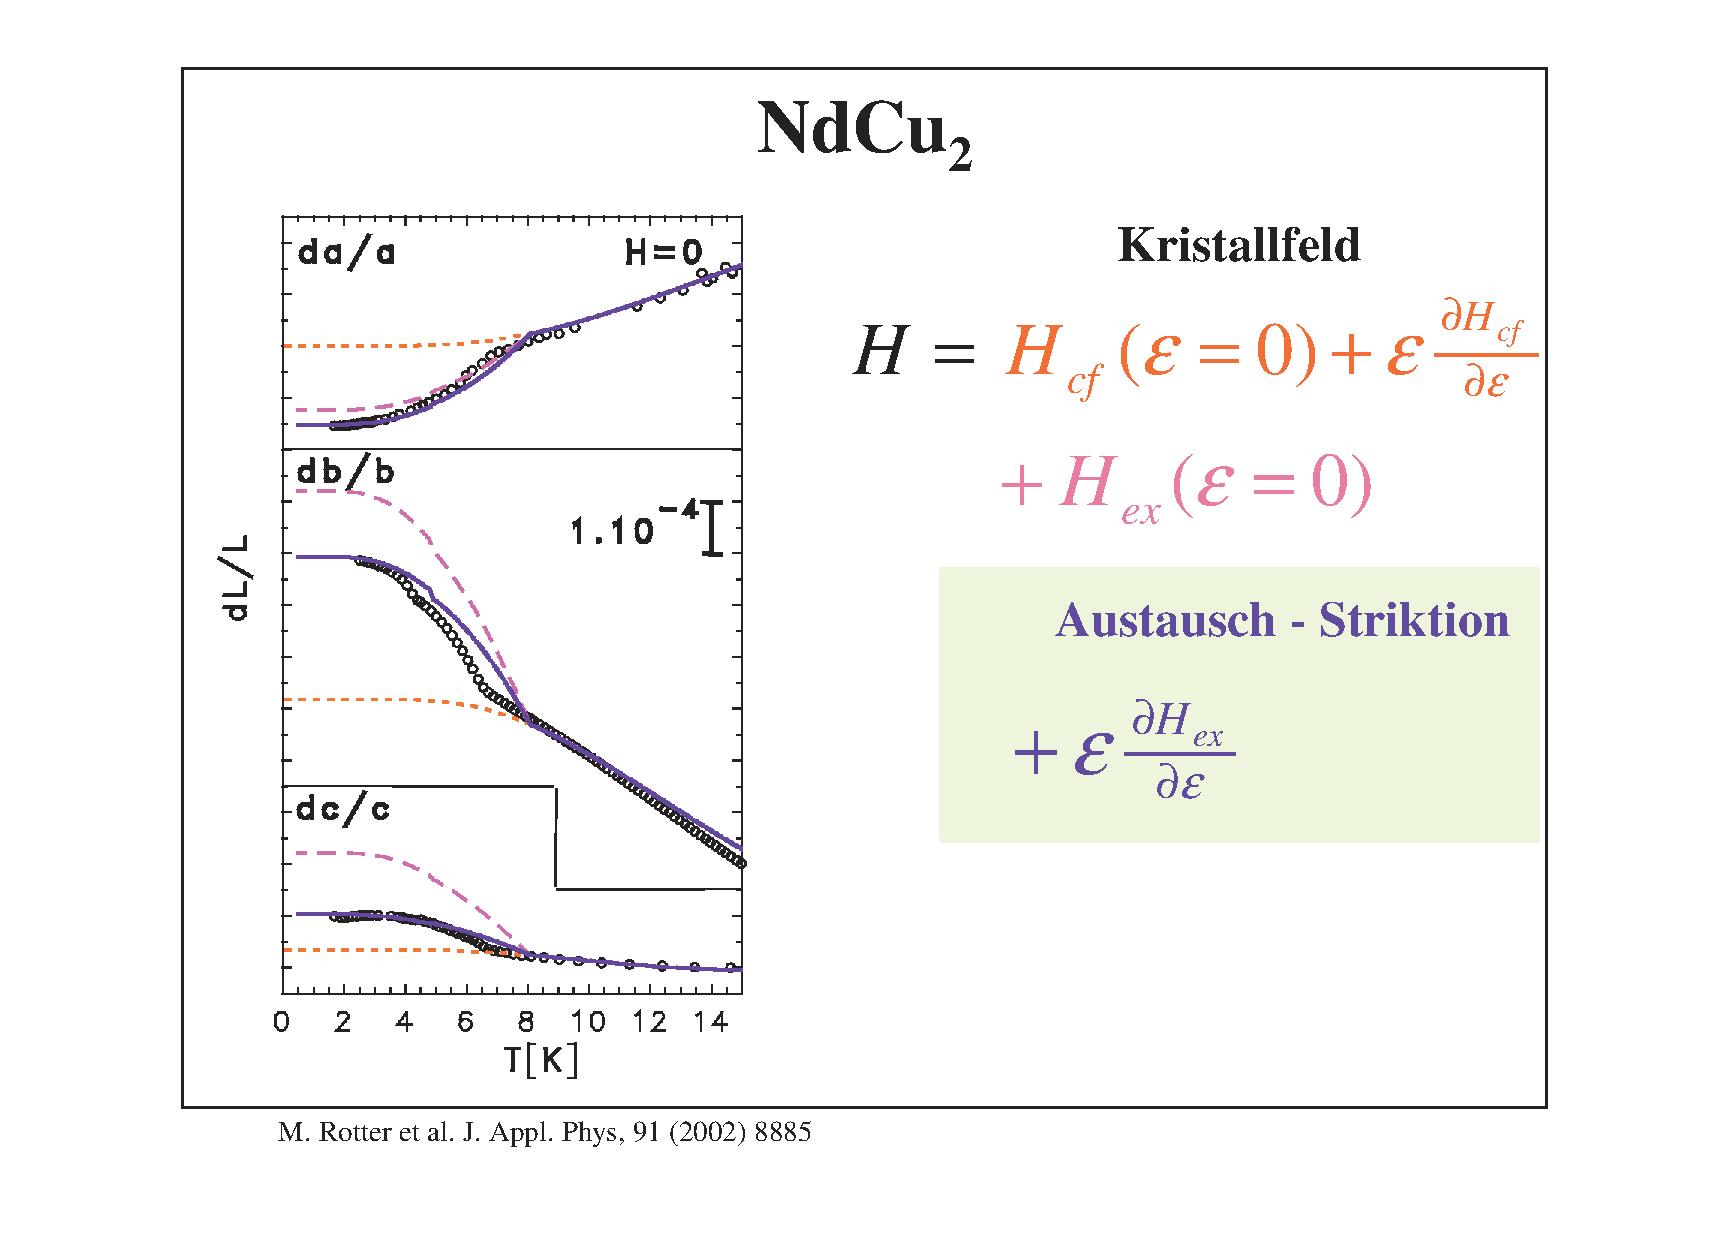
\includegraphics[angle=0, width=0.8\textwidth]{figsrc/magnetostriction_ndcu2.eps}
\end{center}
\caption{Calculated spontaneous magnetostriction of NdCu$_2$.}
\label{magnetostrictiongraphic}
\end{figure}

\begin{description}
\item [\prg mcphas.qvc]    the set of test q-vectors used for calculation of free energy.
                           Components of these q vectors refer to the reciprocal lattice $\vec a^*,\vec b^*,\vec c^*$.
\item [\prg mcphas.phs]    spin-configuration table of different types of spin-configurations. 
                            Note, in case of non-orthogonal axes the convention in these tables 
                            is $mb||\vec b$, $mc||(\vec a \times \vec b)$ and $ma$ perpendicular to $mb$ and $mc$.

                           {\em Note}: 
                           there is no natural criteria for deciding, if one spin-configuration is
			   different from another one. Therefore the list of ''different''
			   spin-configurations is dependent on the meaning of ''different''.
			   
			   The program {\prg McPhase} decides whether a spin-configuration is
			   different from another by a simple criteria, namely by the
			   angle between the spins. Comparing two spin configurations it calculates
			   the angle between corresponding spins and if for one spin the
			   angle is not small, the configuration is treated as a different
			   configuration. Therefore for example a ferromagnet with moments
			   in $a$ has a different spin configuration than a ferromagnet with
			   moments in $b$ direction. 
\item [\prg mcphas.sps]    $T-H$ dependence of spin-configuration. The spin configurations stored in this
                           file may be displayed using the program {\prg spins\index{spins}}, an example is given
			   in figure~\ref{spingraphic}.
                            Note, in case of non-orthogonal axes the convention for applied field $Ha, Hb,Hc$ and
                            also for the moment components $ma, mb, mc$ in these tables 
                            is $mb||\vec b$, $mc||(\vec a \times \vec b)$ and $ma$ perpendicular to $mb$ and $mc$.

\item [\prg mcphas.mf]     $T-H$ dependence of exchange field configuration, stored as $g_J \mu_B H_{xc}(i)$(unit is in meV)
                            for i=1,2,...,number of spins in magnetic unit cell.
                            Note, in case of non-orthogonal axes the convention for applied field $Ha, Hb,Hc$ and
                            also for the mean field components in these tables 
                            is $Hb||\vec b$, $Hc||(\vec a \times \vec b)$ and $Ha$ perpendicular to $Hb$ and $Hc$.
\item [\prg mcphas.fum]    free energy, magnetic energy (the derivative with respect to temperature gives the specific %%@
heat),
                           magnetisation data and (if cfield is used with higher order interactions)
                           expectation values of the Stevens Operators $<O_l^m>$ . As an example for the information
			   contained in this file the calculated magnetisation and magnetostriction of NdCu$_2$ is shown in
			   figures~\ref{magnetization} and ~\ref{magnetizationgraphic}.
                            Note, in case of non-orthogonal axes the convention for applied field $Ha, Hb,Hc$ and
                            also for the magnetisation components $ma,mb,mc$ in these tables 
                            is $Hb||\vec b$, $Hc||(\vec a \times \vec b)$ and $Ha$ perpendicular to $Hb$ and $Hc$.

\item [\prg mcphas1.j1 .j1 .j2 ...] 
               spin-spin correlation functions for sub-lattice 1 neighbour 1 2 ...
	       (linear combination is proportional to magnetostriction)
	       The spin-spin correlation functions for neighbour $k$ are defined by
	       the following sum of dyadic products:

	       \begin{equation}
	        \frac{1}{n}\sum_{s=1}^n <{\mbf J}^s> \times  <{\mbf J}^{s+k}>
	       \end{equation}
	       with $n$ being the number of moments in the magnetic unit cell.
	       Single ion and two-ion magnetostriction can be calculated using the $<O_l^m>$ and the
	       spin-spin correlation functions. As an example the magnetostriction analysis of
	       NdCu$_2$ is shown in figure~\ref{magnetostrictiongraphic}. For details 
             please refer to~\cite{rotter02-8885}.
                            Note, in case of non-orthogonal axes the convention for applied field $Ha, Hb,Hc$ and
                            also for the moment components in these tables 
                            is $Hb||\vec b$, $Hc||(\vec a \times \vec b)$ and $Ha$ perpendicular to $Hb$ and $Hc$.
\item [\prg mcphas.xyt]    phase diagram as x,y,T, H, phase-number j according to spin-configuration table
               given in mcphas.phs, a periodicity key, nettomoments <J>.
 Figure~\ref{phasediagramgraphic}
	       shows the phase diagram of NdCu$_2$ for magnetic fields parallel to the orthorhombic $b$-direction.
                            Note, in case of non-orthogonal axes the convention for applied field $Ha, Hb,Hc$ 
                             in these tables 
                            is $Hb||\vec b$, $Hc||(\vec a \times \vec b)$ and $Ha$ perpendicular to $Hb$ and $Hc$.
\item [\prg mcphas.hkl]    calculated (unpolarised) neutron diffraction data (the calculated magnetic intensities
    correspond to the magnetic structure + Polarisation factor. The
    Lorentz-factor , magnetic form factor and  instrumental corrections are not calculated.)
 As an example figure~\ref{neutintgraphic}
    shows the calculated temperature dependence of magnetic amplitudes for NdCu$_2$.
                           $h,k,l$ refer to the reciprocal lattice $\vec a^*,\vec b^*,\vec c^*$.
                            Note, in case of non-orthogonal axes the convention for applied field $Ha, Hb,Hc$ 
                             in these tables 
                            is $Hb||\vec b$, $Hc||(\vec a \times \vec b)$ and $Ha$ perpendicular to $Hb$ and $Hc$.
    
\item [\prg mcphasa.hkl]    Fourier Transform of the $a$-component of the magnetic Moments.
                           $h,k,l$ refer to the reciprocal lattice $\vec a^*,\vec b^*,\vec c^*$.
                            Note, in case of non-orthogonal axes the convention for applied field $Ha, Hb,Hc$ and
                            the magnetic moment component in these tables 
                            is $Hb||\vec b$, $Hc||(\vec a \times \vec b)$ and $Ha$ perpendicular to $Hb$ and $Hc$.
\item [\prg mcphasb.hkl]    Fourier Transform of the $b$-component of the magnetic Moments.
                           $h,k,l$ refer to the reciprocal lattice $\vec a^*,\vec b^*,\vec c^*$.
                            Note, in case of non-orthogonal axes the convention for applied field $Ha, Hb,Hc$ and
                            the magnetic moment component in these tables 
                            is $Hb||\vec b$, $Hc||(\vec a \times \vec b)$ and $Ha$ perpendicular to $Hb$ and $Hc$.
\item [\prg mcphasc.hkl]    Fourier Transform of the $c$-component of the magnetic Moments.
                           $h,k,l$ refer to the reciprocal lattice $\vec a^*,\vec b^*,\vec c^*$.
                            Note, in case of non-orthogonal axes the convention for applied field $Ha, Hb,Hc$ and
                            the magnetic moment component in these tables 
                            is $Hb||\vec b$, $Hc||(\vec a \times \vec b)$ and $Ha$ perpendicular to $Hb$ and $Hc$.
\end{description} 

\vspace{1cm}
{\em Exercises:}
\begin{itemize}
\item Look at the output files of {\prg McPhase}  in the directory
{\prg examples/ndcu2b\_new/results}.  At which magnetic field
the ferromagnetically aligned state is achieved (at $T=$2~K)?
\item
What is the propagation vector in the different antiferromagnetic phases at $T=$2~K ?
\end{itemize}





\subsubsection{{\prg mcphas.j\index{mcphas.j}} - lattice and exchange parameters}\label{mcphasj}
This file provides the information about 
the crystallographic
 structure and the magnetic exchange interactions.
For every atom in the crystallographic basis there
has to be given the coordinates, the number of neighbours to be considered, the 
Land\'e factor $g_J$, the single ion property filename and  a set of exchange parameters.
If the exchange parameters (and neighbour positions) are not known for your system, you 
can use the program module {\prg makenn\index{makenn}} (see section \ref{addprog}) to generate 
a list of nearest neighbours and
exchange parameters, currently implemented in {\prg makenn\index{makenn}} are dipolar interactions,
exchange interactions via the Bethe-Slater curve or the RKKY model. Note that in order
to use {\prg makenn\index{makenn}} you have to set up a working {\prg mcphas.j\index{mcphas.j}} file, which may or
may not contain neighbours and interactions.

Use program {\prg addj\index{addj}} to add exchange parameter set stored in different 
such {\prg .j} files (see section~\ref{addprog}).



\begin{description}
\item [Line 1,2:] Comment Lines
\item [Line 3:] lattice constants a,b,c and crystal angles alpha, beta, gamma 
\item [Line 4-6:] primitive lattice vectors
\item [Line 7:] Number of atoms in the primitive crystallographic unit cell ({\prg nofatoms})
\item [Line 8:] a comment line with stars
\item [Line 9:] coordinates  ($d_a$,$d_b$,$d_c$) of 1$^{st}$ magnetic ion in the crystallographic unit cell  with
respect to the lattice vectors $\vec a$,$\vec b$,$\vec c$. The number of neighbours of this 
ion, for which interaction constants are given in the interaction table (nofneighbours). 
If {\prg diagonalexchange}
is set to 0 the 9 components of the exchange tensor are given in column 4-12. 
If {\prg diagonalexchange}
 is 1, only 3 components are given (column 4-6).
If {\prg diagonalexchange}
 is 2, specific components of the exchange tensor can be given in columns 4 onwards. The indices of these components
 must be given in the following line (Line 9a below).
The Land\'e factor of the ion (gJ) and the file name of the corresponding single ion
parameter file (cffilename).
\item [Line 9a:]  If {\prg diagonalexchange=2}, then this line gives the indices of the exchange tensor corresponding to 
 the columns 4 onwards. It must have a variable called {\prg indexexchange} followed by a list of names of components of the interaction
 tensor separated by space. E.g.
 \verb|  #! indexexchange= JaJb JbJc  | 
means column 4 gives the the interaction constant between the
 first angular momentum component of the current ion with the second angular momentum component of its neighbour, whilst 
 column 5 has the interaction constant between the second angular momentum component of this ion with the third component of its
 neighbour. Alternatively, pairs of numbers may be given, as in \verb|  #! indexexchange= 1,2 2,3  |
 Additionally another parameter {\prg symmetricexchange} can be set to 1, where the value in each column is also used 
 for the transposed tensor component. Thus \verb|  #! symmetricexchange=1 indexexchange= JaJb  | is the same as \\
 \verb|  #! indexexchange= JaJb JbJa  | where the 4th and 5th column are the same.
\item [Line 10:]  Comment line
\item [Line 11-(10+nofneighbours):] Interaction table for ion number 1.   
Note: the neighbour coordinates (column 1-3) are given with respect to the lattice vectors
$\vec a$,$\vec b$,$\vec c$. The program then calculates from these values the coordinates
with respect to the primitive lattice $\vec r_1$,~$\vec r_2$,~$\vec r_3$.
($ d_a \vec a + d_b \vec b + d_c \vec c = d_1 \vec r_1 + d_2 \vec r_2 + d_3 \vec r_3$).
Column 4,5,6 \dots contain the components of the interaction tensor $\stackrel{=}{\mathcal J}$. 
Note that in case of non-orthogonal axes the 
components of the moments and the interaction tensor $Ja, Jb, Jc, Jaa, Jbb, Jcc, Jab ...$ 
refer to the orthogonal coordinate system
defined with respect to the nonorthogonal lattice $\vec a,\vec b,\vec c$ as
$Jb||\vec b$, $Jc||(\vec a \times \vec b)$ and $Ja$ perpendicular to $Jb$ and $Jc$.
\item [Line (11+nofneighbours) - end:] for each ion in the unit cell line 8 - (10+nofneighbours)
are repeated.
\end{description}


\vspace{0.5cm}

{\small {\bf Information for experienced users:}
\begin{description}
\item[\prg mcphas.jjj:]
format of exchange parameter file, which only needs a reduced set of exchange
parameters in the input file. Using the program {\prg jjj2j} the file can be transformed
to {\prg mcphas.j\index{mcphas.j}} by adding lines for all the equivalent neighbours. The format definition
of {\prg mcphas.jjj} is the same as {\prg mcphas.j\index{mcphas.j}}, however each line denotes several
equivalent neighbour atoms (instead of only one in {\prg mcphas.j\index{mcphas.j}}) according to the
 following rules:
\begin{itemize}
\item If a nonzero coordinate $d_a$ (or $d_b$,$d_c$) in the interaction table
 corresponds to it's value at the nearest
 lattice point of the primitive lattice,
  additional interactions of the same size
with  neighbours with coordinate $-d_a$ (or $-d_b$,$-d_c$, respectively)
are taken into account. This
holds for each of the three coordinates $d_a$,$d_b$ and $d_c$
 resulting in a maximum
number of 8 equivalent neighbours per line in the interaction table.
\item If the value of $d_a$ (or $d_b$,$d_c$) is zero or differs
from it's value at the nearest lattice point of the primitive lattice, it is 
changed to the value at the nearest lattice point and {\bf no} interaction 
with  neighbours with coordinates $-d_a$ (or $-d_b$,$-d_c$) is
 taken into account. If such
 interaction is needed it may be given in a different line and may
have different magnitude. In this way also crystallographic lattices
with no mirror symmetry may be described.
\end{itemize}
\item[\prg mcphas.coq:]   exchange parameters etc [ in old format]...see examples for details, use {\prg coq2jjj} to 
transform {\prg mcphas.coq} to {\prg mcphas.jjj} format
\end{description}

}


\subsubsection{Example {\prg mcphas.j\index{mcphas.j}} file for a simple antiferromagnet}

Here are example files of a tetragonal antiferromagnet with nearest neighbour interactions, all
files are equivalent:

{\small
\begin{verbatim} 
# simple antiferromagnet 
#<!--mcphase.mcphas.j-->
#***************************************************************
# Lattice Constants (A)
#! a=4.3843 b=4.3843 c=2.4194 alpha=  90 beta=  90 gamma=  90
#! r1a=   1 r2a=   0 r3a=   0
#! r1b=   0 r2b=   1 r3b=   0   primitive lattice vectors [a][b][c]
#! r1c=   0 r2c=   0 r3c=   1
#! nofatoms=1  nofcomponents=3  number of atoms in primitive unit cell/number of components of each spin
# ****************************************************************************
#! da=  0 [a] db=  0 [b] dc=  0 nofneighbours=2 diagonalexchange=0 gJ=0.857143 cffilename=Ce3p.sipf
# da[a] db[b] dc[c] Jaa[meV] Jbb[meV] Jcc[meV] Jab[meV] Jba[meV] Jac[meV] Jca[meV] Jbc[meV] Jcb[meV]
+0	+0	+1	-0.1	-0.1	-0.1   0  0  0  0  0  0
+0	+0	-1	-0.1	-0.1	-0.1   0  0  0  0  0  0
#\end{verbatim}
}

Using diagonalexchange this may be shortened to

{\small
\begin{verbatim} 
# simple antiferromagnet 
#<!--mcphase.mcphas.j-->
#***************************************************************
# Lattice Constants (A)
#! a=4.3843 b=4.3843 c=2.4194 alpha=  90 beta=  90 gamma=  90
#! r1a=   1 r2a=   0 r3a=   0
#! r1b=   0 r2b=   1 r3b=   0   primitive lattice vectors [a][b][c]
#! r1c=   0 r2c=   0 r3c=   1
#! nofatoms=1  nofcomponents=3  number of atoms in primitive unit cell/number of components of each spin
# ****************************************************************************
#! da=  0 [a] db=  0 [b] dc=  0 nofneighbours=2 diagonalexchange=1 gJ=0.857143 cffilename=Ce3p.sipf
# da[a] db[b] dc[c] Jaa[meV] Jbb[meV] Jcc[meV] Jab[meV] Jba[meV] Jac[meV] Jca[meV] Jbc[meV] Jcb[meV]
+0	+0	+1	-0.1	-0.1	-0.1   
+0	+0	-1	-0.1	-0.1	-0.1   
#\end{verbatim}
}

with indexexchange option the sequence of two ion interaction parameters can be changed and
zero parameters may be omitted:

{\small
\begin{verbatim} 
# simple antiferromagnet 
#<!--mcphase.mcphas.j-->
#***************************************************************
# Lattice Constants (A)
#! a=4.3843 b=4.3843 c=2.4194 alpha=  90 beta=  90 gamma=  90
#! r1a=   1 r2a=   0 r3a=   0
#! r1b=   0 r2b=   1 r3b=   0   primitive lattice vectors [a][b][c]
#! r1c=   0 r2c=   0 r3c=   1
#! nofatoms=1  nofcomponents=3  number of atoms in primitive unit cell/number of components of each spin
# ****************************************************************************
#! da=  0 [a] db=  0 [b] dc=  0 nofneighbours=2 diagonalexchange=2 gJ=0.857143 cffilename=Ce3p.sipf
# da[a] db[b] dc[c] Jaa[meV] Jbb[meV] Jcc[meV] Jab[meV] Jba[meV] Jac[meV] Jca[meV] Jbc[meV] Jcb[meV]
#! indexexchange = JaJa JaJc JcJa JbJb JcJc
+0	+0	+1	-0.1 0 0 -0.1	-0.1  
+0	+0	-1	-0.1 0 0 -0.1	-0.1  
#\end{verbatim}
}

{\small
\begin{verbatim} 
# simple antiferromagnet 
#<!--mcphase.mcphas.j-->
#***************************************************************
# Lattice Constants (A)
#! a=4.3843 b=4.3843 c=2.4194 alpha=  90 beta=  90 gamma=  90
#! r1a=   1 r2a=   0 r3a=   0
#! r1b=   0 r2b=   1 r3b=   0   primitive lattice vectors [a][b][c]
#! r1c=   0 r2c=   0 r3c=   1
#! nofatoms=1  nofcomponents=3  number of atoms in primitive unit cell/number of components of each spin
# ****************************************************************************
#! da=  0 [a] db=  0 [b] dc=  0 nofneighbours=2 diagonalexchange=2 gJ=0.857143 cffilename=Ce3p.sipf
# da[a] db[b] dc[c] Jaa[meV] Jbb[meV] Jcc[meV] Jab[meV] Jba[meV] Jac[meV] Jca[meV] Jbc[meV] Jcb[meV]
#! indexexchange = 1,1 1,3, 3,1 2,2 3,3
+0	+0	+1	-0.1 0 0 -0.1	-0.1  
+0	+0	-1	-0.1 0 0 -0.1	-0.1  
#\end{verbatim}
}


using symmetricexchange together with indexexchange will assume that the interaction tensor is symmetic and 
only half of it may be given:

{\small
\begin{verbatim} 
# simple antiferromagnet 
#<!--mcphase.mcphas.j-->
#***************************************************************
# Lattice Constants (A)
#! a=4.3843 b=4.3843 c=2.4194 alpha=  90 beta=  90 gamma=  90
#! r1a=   1 r2a=   0 r3a=   0
#! r1b=   0 r2b=   1 r3b=   0   primitive lattice vectors [a][b][c]
#! r1c=   0 r2c=   0 r3c=   1
#! nofatoms=1  nofcomponents=3  number of atoms in primitive unit cell/number of components of each spin
# ****************************************************************************
#! da=  0 [a] db=  0 [b] dc=  0 nofneighbours=2 diagonalexchange=2 gJ=0.857143 cffilename=Ce3p.sipf
# da[a] db[b] dc[c] Jaa[meV] Jbb[meV] Jcc[meV] Jab[meV] Jba[meV] Jac[meV] Jca[meV] Jbc[meV] Jcb[meV]
#! symmetricexchange=1 indexexchange = JaJa JaJc JbJb JcJc
+0	+0	+1	-0.1 0  -0.1	-0.1  
+0	+0	-1	-0.1 0  -0.1	-0.1  
#\end{verbatim}
}


\subsubsection{Single Ion Property Input Files}\label{sifile}

In order to speed up calculations or treat special problems a large 
variety of single ion modules is available. This includes the
option to load a user written single ion module. Details are 
given in chapter~\ref{simod}.

The first time user of {\prg McPhase} should use the module {\prg so1ion}\index{so1ion} and 
create an appropriate single ion property input file as described in
section \ref{cf1ion}. A good starting point are several examples
given in directory {\prg examples}.


\subsubsection{Example single ion property file  for a simple antiferromagnet}

Here is an example file {\prg mcphas.cf1} describing the anisotropy of a 
simple antiferromagnet with Ce atoms having basal plane anisotropy. Note the
axis convention xyz$||$abc, in case of non-orthogonal axes the convention 
is $y||\vec b$, $z||(\vec a \times \vec b)$ and $x$ perpendicular to $y$ and $z$.


\section{{\prg mcphas} - calculation of thermodynamic properties (Magnetisation, Susceptibility, Specific Heat, Neutron %%@
Diffraction, etc.)}
\label{runmcphas}

In order to perform calculations beyond the capabilities of {\prg cfield\index{cfield}} it is necessary
to use the program {\prg mcphas}. 
\begin{itemize}
\item As a first step it is possible to
calculate the thermodynamic properties such as magnetisation or specific heat
considering only single ion effects. In this case all the exchange parameters
have to be set to zero in {\prg mcphas.j\index{mcphas.j}}. 
\item for more advanced calculations the two - ion interactions have to be
considered and may lead to magnetic order. {\prg mcphas} can perform 
calculations in the ordered state in the following way: for 
a given temperature $T$ and magnetic field $\mbf H$ (vector)
several possible magnetic structures are stabilised
by a mean field algorithm and the free energy is 
calculated. The initial values for this mean-field procedure are
modified by a Monte Carlo process.


The temperature and magnetic field is varied during the calculation
and thereby it is possible to map out the magnetic phase diagram.
\end{itemize}

The program produces a plot of the stabilised magnetic
structures and the magnetisation on screen, the
output files contain additional information 
such as calculated magnetoelastic and  neutron-scattering
data. Several graphic programs easy the visualisation of the
calculated data (section~\ref{graphics}).



\subsection{Input Files}
The program {\prg McPhase} needs the following input files (all in the same directory)
 in order to run:

\begin{enumerate}
\item {\prg mcphas.ini\index{mcphas.ini}}
 - controlling the algorithm
\item {\prg mcphas.j\index{mcphas.j}}
  - lattice and exchange parameters
\item {\prg mcphas.tst\index{mcphas.tst}(optional)}  - test spin configurations
\item {\prg single-ion property files}
\item {\prg directory ./results/}
 - directory where calculated data is stored
\item {\prg directory ./fit} - experimental data for fit (optional)
\end{enumerate}


 All
 of these input files have to be in one directory and the program
has to be started in this directory. The results of the simulation
are then stored in the  subdirectory ./results/, which must exist before starting
the program 
... see directory ./examples/ for some examples.
 In order to prepare these files
for a new calculation it is best to take them from an example, copy the files
to a new directory and make the
modifications  to adapt them to the new problem.

\subsubsection{Example - a simple antiferromagnet}

In the following description of the input files we will always refer
to a simple example: a simple antiferromagnet
on a primitive orthorhombic lattice. The first time user
will thus have a simple example to follow, all corresponding
files are given in the directory {\prg tutorial/03magnetic\_phases\_mcphas/simpleAF}.
 

\subsubsection{{\prg mcphas.ini\index{mcphas.ini}} - controlling the algorithm}
   Initial file containing algorithm control parameters, for instance the range and spacing of
   propagation vectors Q or the number of Monte Carlo trials for initial spin configurations
    - {\em mind}: this
   file is rewritten and reread  when running the program and may be changed by the
   user in order to manipulate the running simulation.

{\prg mcphas.ini\index{mcphas.ini}} consists of several sections:
\begin{description}
\item [MCPHASE RUNTIME CONTROL:] this section contains the parameters
controlling the status of the calculation.
\item [XY PHASEDIAGRAM PARAMETERS:] here the temperature and field range and
step widths of the calculation are specified.
The definition of the x and y
axis in terms of temperature and magnetic field is followed by the
corresponding range and step width. An offset may be given for all
field and temperature values.
Note that for most cases of interest
this offset is zero (T0=0, Ha0=0, Hb0=0, Hc0=0).
 For the simple case of calculating a Temperature-Field phase diagram
 It is just necessary to set xT=1 and give the temperature range by
xmin/xmax/xstep. For field in b direction then just set yHb=1 and 
define the range in ymin/ymax/ystep.
In case of non-orthogonal axes the applied magnetic field
components $Ha, Hb, Hc$ refer to the orthogonal coordinate system
defined with respect to the nonorthogonal lattice $\mbf a,\mbf b,\mbf c$ as
$Hb||\mbf b$, $Hc||(\mbf a \times \mbf b)$ and $Ha$ perpendicular to $Hb$ and $Hc$.

\item [GENERATION OF SPINCONFIGURATIONS:] at the beginning of the program
some initial values of spin configurations are generated from a set of 
propagation vectors. This section defines the range of propagation vectors
and the step width.
Depending on the value of the propagation Q with respect to the primitive reciprocal lattice
1-, 2- or 3-dimensional simulations of magnetic lattices
are possible. It is advisable to 
think carefully about the chosen range and spacing of Q vectors in order
to limit calculation time.
 
For example a good starting point is to begin with a calculation with large
step widths (e.g. 0.1)  covering the Brillouin zone. This should give an idea
of the propagation vectors which are stabilised. An advanced calculation
could then fine tune the propagation and determine its accurate value (using
small step widths in a limited area of the zone).
The verbose option of {\prg mcphas} allows to inspect the propagation vectors
which are actually used in the calculation.
Trick: in order to get a quick overview of the
q-vector range covered by the mcphas\index{mcphas} simulation start mcphas, exit and 
just type {\prg felog ./results/mcphas.qvc} (need {\prg perl,perldl,pdl,pgplot} packages).

In order to limit calculation time, the maximum periodicity
of the magnetic unit cell with respect to the crystallographic unit cell 
(maxqperiod) and the maximum number of spins in the magnetic unit cell 
(maxnofspins) can be limited. Also the maximum number of test spin configurations
in the internal table can be limited (maxnoftestspincf).
A critical feature with respect to calculation time is also the number of
spin configurations which are generated by a random process from a tabulated
SPINCONFIGURATIONS during the calculation. 

In summary the variables in this section are mainly important to adapt the
program to a given computer system with finite speed. They have to be set
to optimise between speed and accuracy of the calculation. In order to
find appropriate values it is best to perform some calculations 
and restrict the parameters step by step if insufficient speed is obtained.
Also the examples included in the program package may serve as starting
points.

\item [PARAMETERS FOR SUB FECALC SELFCONSISTENCY PROCESS:] the most important
procedure in the module {\prg mcphas} is the sub fecalc. In this part of the 
program the self consistent calculation of the magnetic moment configuration
is performed as shown schematically in fig.~\ref{fecalc}. 
In the mean field approximation the Hamiltonian~(\ref{hamilton}) is approximated
by

\begin{equation}
 {\mathcal H}=\sum_n H_{SI}^n + E_{corr}
\end{equation}

with the single ion Hamiltonian (in case of module {\prg so1ion\index{so1ion}})

\begin{equation}
H_{SI}^n=  B_l^m O_{lm}({\mbf J}^n) 
	     - g_{Jn} \mu_B {\mbf J}^n {\mbf H^n_{eff}} 
\end{equation}

and the correction term

\begin{equation}
E_{corr}=\frac{1}{2}\sum_{n} g_{Jn} \mu_B \langle {\mbf J}^n
 \rangle (\mbf H^n_{eff}-\mbf H) 
\end{equation}

and with the mean fields $ \mbf H^n_{eff}$ given by

\begin{equation}\label{meanfield}
\mbf H^n_{eff}=\mbf H + \mbf H^n_{xc}=\mbf H+\sum_{{\mbf G'}n'} \frac{{\mathcal J}
(\mbf r_n-(\mbf G'+\mbf r_{n'}))}{g_{Jn}\mu_B } \langle{\mbf
J}^{n'}\rangle
\end{equation}

These mean fields and the moments $\langle \mbf J^n \rangle$ 
are determined in a self consistent
way. For a given magnetic unit cell and initial configuration 
of magnetic moments
the mean fields are calculated according to equation~(\ref{meanfield}). 
Then, for each
magnetic ion the single ion property module is taken 
and the magnetic moment $\langle \mbf J^n \rangle$ is 
calculated from it's mean field. The mean fields are used again in equation~(\ref{meanfield})
and so on .... until convergence is reached. 
Then, the free energy ($f=-kT\sum_n \ln(z_n) + E_{corr}$ ) 
of the stabilised
configuration is calculated (this is why this sub is called {\prg fecalc}). 
The free energies of a lot of different stabilised configurations have to
be compared in order to find out which configuration has lowest free energy, i.e.
is stable in thermal  equilibrium.

It may happen that this process does
not converge due to bad choice of the initial configuration, therefore a maximum number
of mean field loops has to be given by the user.
The results of a calculation may be significantly influenced by
changing parameters such as the maximum number of iteration loops 
in this section. 
In fact the simulation is always a compromise of calculation time and accuracy: if only
a few initial spin configurations are tried at each (H-T) point, the calculation speed is
fast, however it is possible that the program misses the magnetic structure with the
lowest free energy. The same holds if other critical parameters of the simulation are
restricted too much.
 

\item [OUTPUT OF PHYSICAL PROPERTIES:]
Some options for the output of the calculation can be changed in this section.
\end{description}

\begin{figure}[hb]
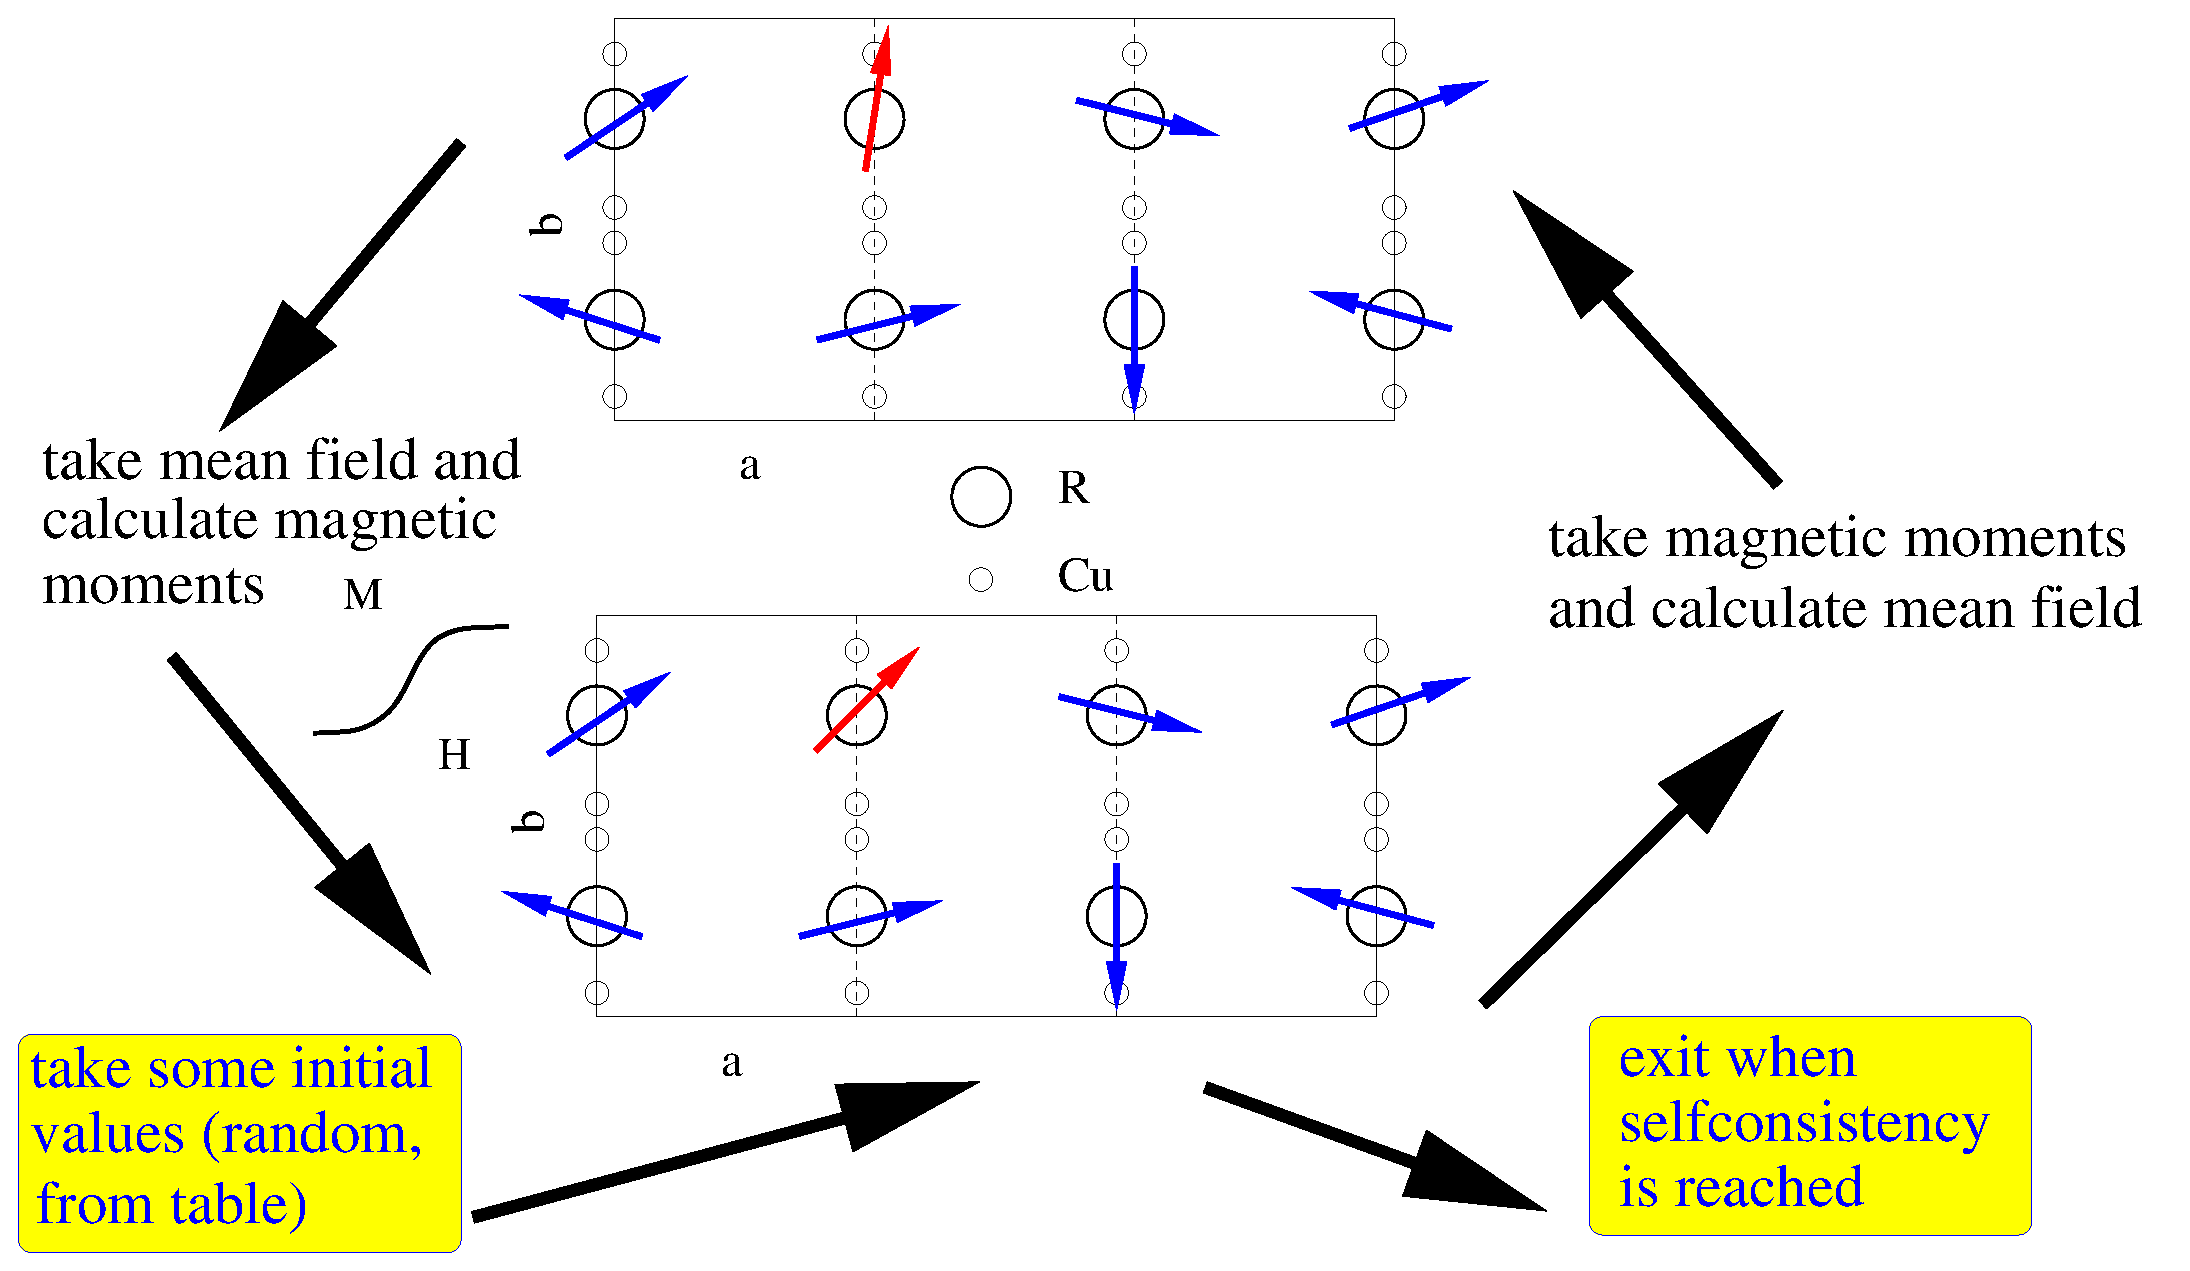
\includegraphics[angle=0,width=0.9\columnwidth]{figsrc/fecalc.eps}
\caption{\label{fecalc}Mean field process of sub {\prg fecalc}.}
\end{figure}

 
\subsubsection{Example {\prg mcphas.ini\index{mcphas.ini}} file for a simple antiferromagnet}

Here is an example of {\prg mcphas.ini\index{mcphas.ini}}, the comments describe the meaning of the different
parameters:

\section{{\prg mcphas} - calculation of thermodynamic properties (Magnetisation, Susceptibility, Specific Heat, Neutron %%@
Diffraction, etc.)}
\label{runmcphas}

In order to perform calculations beyond the capabilities of {\prg cfield\index{cfield}} it is necessary
to use the program {\prg mcphas}. 
\begin{itemize}
\item As a first step it is possible to
calculate the thermodynamic properties such as magnetisation or specific heat
considering only single ion effects. In this case all the exchange parameters
have to be set to zero in {\prg mcphas.j\index{mcphas.j}}. 
\item for more advanced calculations the two - ion interactions have to be
considered and may lead to magnetic order. {\prg mcphas} can perform 
calculations in the ordered state in the following way: for 
a given temperature $T$ and magnetic field $\mbf H$ (vector)
several possible magnetic structures are stabilised
by a mean field algorithm and the free energy is 
calculated. The initial values for this mean-field procedure are
modified by a Monte Carlo process.


The temperature and magnetic field is varied during the calculation
and thereby it is possible to map out the magnetic phase diagram.
\end{itemize}

The program produces a plot of the stabilised magnetic
structures and the magnetisation on screen, the
output files contain additional information 
such as calculated magnetoelastic and  neutron-scattering
data. Several graphic programs easy the visualisation of the
calculated data (section~\ref{graphics}).



\subsection{Input Files}
The program {\prg McPhase} needs the following input files (all in the same directory)
 in order to run:

\begin{enumerate}
\item {\prg mcphas.ini\index{mcphas.ini}}
 - controlling the algorithm
\item {\prg mcphas.j\index{mcphas.j}}
  - lattice and exchange parameters
\item {\prg mcphas.tst\index{mcphas.tst}(optional)}  - test spin configurations
\item {\prg single-ion property files}
\item {\prg directory ./results/}
 - directory where calculated data is stored
\item {\prg directory ./fit} - experimental data for fit (optional)
\end{enumerate}


 All
 of these input files have to be in one directory and the program
has to be started in this directory. The results of the simulation
are then stored in the  subdirectory ./results/, which must exist before starting
the program 
... see directory ./examples/ for some examples.
 In order to prepare these files
for a new calculation it is best to take them from an example, copy the files
to a new directory and make the
modifications  to adapt them to the new problem.

\subsubsection{Example - a simple antiferromagnet}

In the following description of the input files we will always refer
to a simple example: a simple antiferromagnet
on a primitive orthorhombic lattice. The first time user
will thus have a simple example to follow, all corresponding
files are given in the directory {\prg tutorial/03magnetic\_phases\_mcphas/simpleAF}.
 

\subsubsection{{\prg mcphas.ini\index{mcphas.ini}} - controlling the algorithm}
   Initial file containing algorithm control parameters, for instance the range and spacing of
   propagation vectors Q or the number of Monte Carlo trials for initial spin configurations
    - {\em mind}: this
   file is rewritten and reread  when running the program and may be changed by the
   user in order to manipulate the running simulation.

{\prg mcphas.ini\index{mcphas.ini}} consists of several sections:
\begin{description}
\item [MCPHASE RUNTIME CONTROL:] this section contains the parameters
controlling the status of the calculation.
\item [XY PHASEDIAGRAM PARAMETERS:] here the temperature and field range and
step widths of the calculation are specified.
The definition of the x and y
axis in terms of temperature and magnetic field is followed by the
corresponding range and step width. An offset may be given for all
field and temperature values.
Note that for most cases of interest
this offset is zero (T0=0, Ha0=0, Hb0=0, Hc0=0).
 For the simple case of calculating a Temperature-Field phase diagram
 It is just necessary to set xT=1 and give the temperature range by
xmin/xmax/xstep. For field in b direction then just set yHb=1 and 
define the range in ymin/ymax/ystep.
In case of non-orthogonal axes the applied magnetic field
components $Ha, Hb, Hc$ refer to the orthogonal coordinate system
defined with respect to the nonorthogonal lattice $\mbf a,\mbf b,\mbf c$ as
$Hb||\mbf b$, $Hc||(\mbf a \times \mbf b)$ and $Ha$ perpendicular to $Hb$ and $Hc$.

\item [GENERATION OF SPINCONFIGURATIONS:] at the beginning of the program
some initial values of spin configurations are generated from a set of 
propagation vectors. This section defines the range of propagation vectors
and the step width.
Depending on the value of the propagation Q with respect to the primitive reciprocal lattice
1-, 2- or 3-dimensional simulations of magnetic lattices
are possible. It is advisable to 
think carefully about the chosen range and spacing of Q vectors in order
to limit calculation time.
 
For example a good starting point is to begin with a calculation with large
step widths (e.g. 0.1)  covering the Brillouin zone. This should give an idea
of the propagation vectors which are stabilised. An advanced calculation
could then fine tune the propagation and determine its accurate value (using
small step widths in a limited area of the zone).
The verbose option of {\prg mcphas} allows to inspect the propagation vectors
which are actually used in the calculation.
Trick: in order to get a quick overview of the
q-vector range covered by the mcphas\index{mcphas} simulation start mcphas, exit and 
just type {\prg felog ./results/mcphas.qvc} (need {\prg perl,perldl,pdl,pgplot} packages).

In order to limit calculation time, the maximum periodicity
of the magnetic unit cell with respect to the crystallographic unit cell 
(maxqperiod) and the maximum number of spins in the magnetic unit cell 
(maxnofspins) can be limited. Also the maximum number of test spin configurations
in the internal table can be limited (maxnoftestspincf).
A critical feature with respect to calculation time is also the number of
spin configurations which are generated by a random process from a tabulated
SPINCONFIGURATIONS during the calculation. 

In summary the variables in this section are mainly important to adapt the
program to a given computer system with finite speed. They have to be set
to optimise between speed and accuracy of the calculation. In order to
find appropriate values it is best to perform some calculations 
and restrict the parameters step by step if insufficient speed is obtained.
Also the examples included in the program package may serve as starting
points.

\item [PARAMETERS FOR SUB FECALC SELFCONSISTENCY PROCESS:] the most important
procedure in the module {\prg mcphas} is the sub fecalc. In this part of the 
program the self consistent calculation of the magnetic moment configuration
is performed as shown schematically in fig.~\ref{fecalc}. 
In the mean field approximation the Hamiltonian~(\ref{hamilton}) is approximated
by

\begin{equation}
 {\mathcal H}=\sum_n H_{SI}^n + E_{corr}
\end{equation}

with the single ion Hamiltonian (in case of module {\prg so1ion\index{so1ion}})

\begin{equation}
H_{SI}^n=  B_l^m O_{lm}({\mbf J}^n) 
	     - g_{Jn} \mu_B {\mbf J}^n {\mbf H^n_{eff}} 
\end{equation}

and the correction term

\begin{equation}
E_{corr}=\frac{1}{2}\sum_{n} g_{Jn} \mu_B \langle {\mbf J}^n
 \rangle (\mbf H^n_{eff}-\mbf H) 
\end{equation}

and with the mean fields $ \mbf H^n_{eff}$ given by

\begin{equation}\label{meanfield}
\mbf H^n_{eff}=\mbf H + \mbf H^n_{xc}=\mbf H+\sum_{{\mbf G'}n'} \frac{{\mathcal J}
(\mbf r_n-(\mbf G'+\mbf r_{n'}))}{g_{Jn}\mu_B } \langle{\mbf
J}^{n'}\rangle
\end{equation}

These mean fields and the moments $\langle \mbf J^n \rangle$ 
are determined in a self consistent
way. For a given magnetic unit cell and initial configuration 
of magnetic moments
the mean fields are calculated according to equation~(\ref{meanfield}). 
Then, for each
magnetic ion the single ion property module is taken 
and the magnetic moment $\langle \mbf J^n \rangle$ is 
calculated from it's mean field. The mean fields are used again in equation~(\ref{meanfield})
and so on .... until convergence is reached. 
Then, the free energy ($f=-kT\sum_n \ln(z_n) + E_{corr}$ ) 
of the stabilised
configuration is calculated (this is why this sub is called {\prg fecalc}). 
The free energies of a lot of different stabilised configurations have to
be compared in order to find out which configuration has lowest free energy, i.e.
is stable in thermal  equilibrium.

It may happen that this process does
not converge due to bad choice of the initial configuration, therefore a maximum number
of mean field loops has to be given by the user.
The results of a calculation may be significantly influenced by
changing parameters such as the maximum number of iteration loops 
in this section. 
In fact the simulation is always a compromise of calculation time and accuracy: if only
a few initial spin configurations are tried at each (H-T) point, the calculation speed is
fast, however it is possible that the program misses the magnetic structure with the
lowest free energy. The same holds if other critical parameters of the simulation are
restricted too much.
 

\item [OUTPUT OF PHYSICAL PROPERTIES:]
Some options for the output of the calculation can be changed in this section.
\end{description}

\begin{figure}[hb]
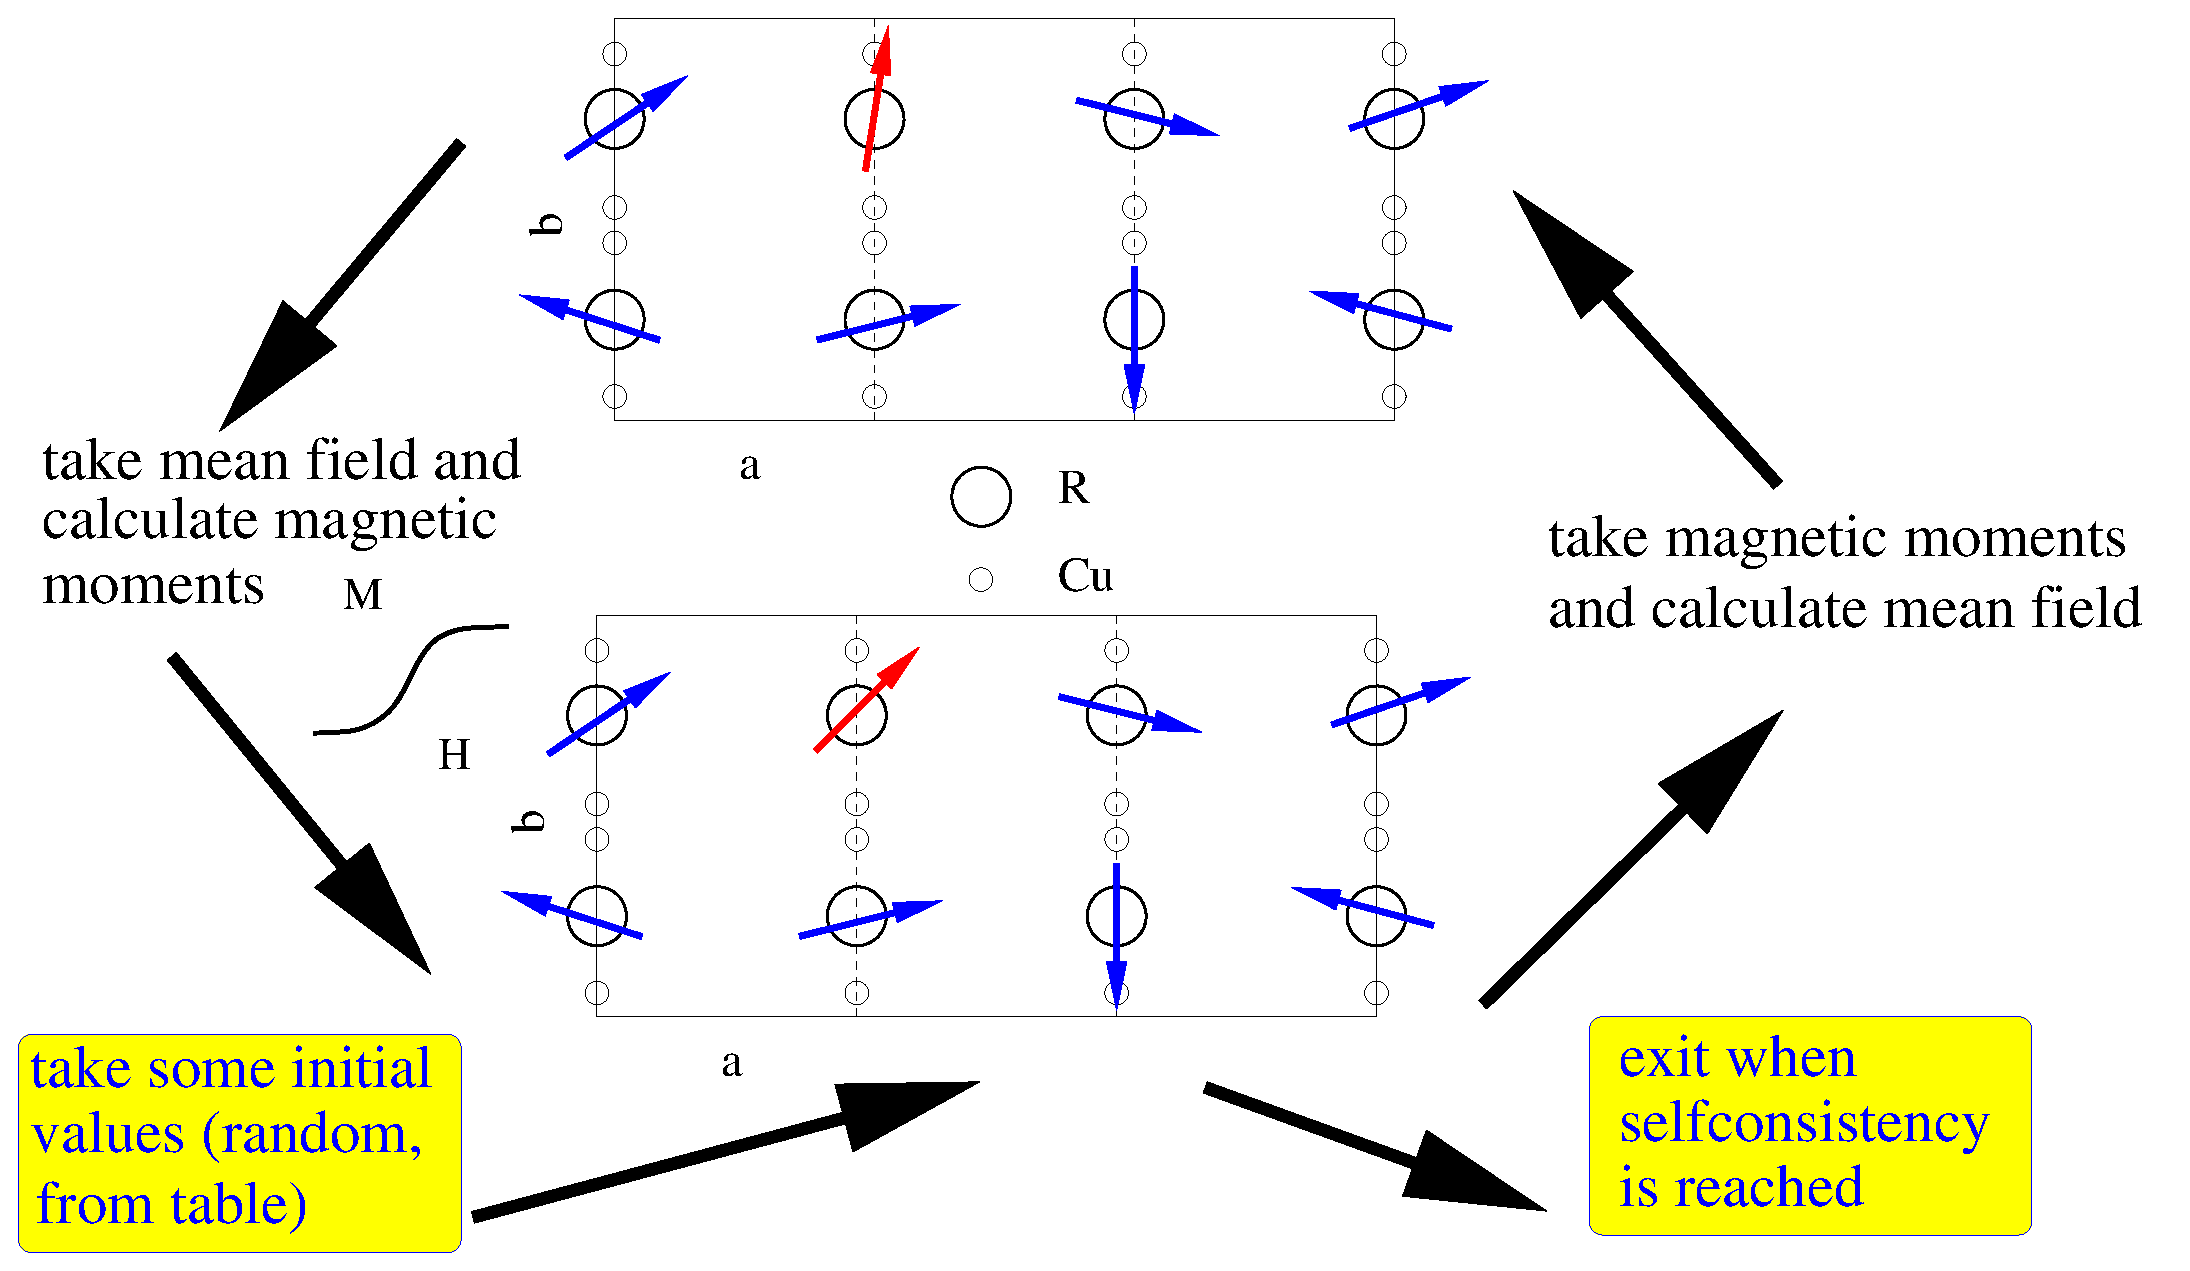
\includegraphics[angle=0,width=0.9\columnwidth]{figsrc/fecalc.eps}
\caption{\label{fecalc}Mean field process of sub {\prg fecalc}.}
\end{figure}

 
\subsubsection{Example {\prg mcphas.ini\index{mcphas.ini}} file for a simple antiferromagnet}

Here is an example of {\prg mcphas.ini\index{mcphas.ini}}, the comments describe the meaning of the different
parameters:

\input{mcphas.ini}



\subsubsection{{\prg mcphas.j\index{mcphas.j}} - lattice and exchange parameters}\label{mcphasj}
This file provides the information about 
the crystallographic
 structure and the magnetic exchange interactions.
For every atom in the crystallographic basis there
has to be given the coordinates, the number of neighbours to be considered, the 
Land\'e factor $g_J$, the single ion property filename and  a set of exchange parameters.
If the exchange parameters (and neighbour positions) are not known for your system, you 
can use the program module {\prg makenn\index{makenn}} (see section \ref{addprog}) to generate 
a list of nearest neighbours and
exchange parameters, currently implemented in {\prg makenn\index{makenn}} are dipolar interactions,
exchange interactions via the Bethe-Slater curve or the RKKY model. Note that in order
to use {\prg makenn\index{makenn}} you have to set up a working {\prg mcphas.j\index{mcphas.j}} file, which may or
may not contain neighbours and interactions.

Use program {\prg addj\index{addj}} to add exchange parameter set stored in different 
such {\prg .j} files (see section~\ref{addprog}).



\begin{description}
\item [Line 1,2:] Comment Lines
\item [Line 3:] lattice constants a,b,c and crystal angles alpha, beta, gamma 
\item [Line 4-6:] primitive lattice vectors
\item [Line 7:] Number of atoms in the primitive crystallographic unit cell ({\prg nofatoms})
\item [Line 8:] a comment line with stars
\item [Line 9:] coordinates  ($d_a$,$d_b$,$d_c$) of 1$^{st}$ magnetic ion in the crystallographic unit cell  with
respect to the lattice vectors $\vec a$,$\vec b$,$\vec c$. The number of neighbours of this 
ion, for which interaction constants are given in the interaction table (nofneighbours). 
If {\prg diagonalexchange}
is set to 0 the 9 components of the exchange tensor are given in column 4-12. 
If {\prg diagonalexchange}
 is 1, only 3 components are given (column 4-6).
If {\prg diagonalexchange}
 is 2, specific components of the exchange tensor can be given in columns 4 onwards. The indices of these components
 must be given in the following line (Line 9a below).
The Land\'e factor of the ion (gJ) and the file name of the corresponding single ion
parameter file (cffilename).
\item [Line 9a:]  If {\prg diagonalexchange=2}, then this line gives the indices of the exchange tensor corresponding to 
 the columns 4 onwards. It must have a variable called {\prg indexexchange} followed by a list of names of components of the interaction
 tensor separated by space. E.g.
 \verb|  #! indexexchange= JaJb JbJc  | 
means column 4 gives the the interaction constant between the
 first angular momentum component of the current ion with the second angular momentum component of its neighbour, whilst 
 column 5 has the interaction constant between the second angular momentum component of this ion with the third component of its
 neighbour. Alternatively, pairs of numbers may be given, as in \verb|  #! indexexchange= 1,2 2,3  |
 Additionally another parameter {\prg symmetricexchange} can be set to 1, where the value in each column is also used 
 for the transposed tensor component. Thus \verb|  #! symmetricexchange=1 indexexchange= JaJb  | is the same as \\
 \verb|  #! indexexchange= JaJb JbJa  | where the 4th and 5th column are the same.
\item [Line 10:]  Comment line
\item [Line 11-(10+nofneighbours):] Interaction table for ion number 1.   
Note: the neighbour coordinates (column 1-3) are given with respect to the lattice vectors
$\vec a$,$\vec b$,$\vec c$. The program then calculates from these values the coordinates
with respect to the primitive lattice $\vec r_1$,~$\vec r_2$,~$\vec r_3$.
($ d_a \vec a + d_b \vec b + d_c \vec c = d_1 \vec r_1 + d_2 \vec r_2 + d_3 \vec r_3$).
Column 4,5,6 \dots contain the components of the interaction tensor $\stackrel{=}{\mathcal J}$. 
Note that in case of non-orthogonal axes the 
components of the moments and the interaction tensor $Ja, Jb, Jc, Jaa, Jbb, Jcc, Jab ...$ 
refer to the orthogonal coordinate system
defined with respect to the nonorthogonal lattice $\vec a,\vec b,\vec c$ as
$Jb||\vec b$, $Jc||(\vec a \times \vec b)$ and $Ja$ perpendicular to $Jb$ and $Jc$.
\item [Line (11+nofneighbours) - end:] for each ion in the unit cell line 8 - (10+nofneighbours)
are repeated.
\end{description}


\vspace{0.5cm}

{\small {\bf Information for experienced users:}
\begin{description}
\item[\prg mcphas.jjj:]
format of exchange parameter file, which only needs a reduced set of exchange
parameters in the input file. Using the program {\prg jjj2j} the file can be transformed
to {\prg mcphas.j\index{mcphas.j}} by adding lines for all the equivalent neighbours. The format definition
of {\prg mcphas.jjj} is the same as {\prg mcphas.j\index{mcphas.j}}, however each line denotes several
equivalent neighbour atoms (instead of only one in {\prg mcphas.j\index{mcphas.j}}) according to the
 following rules:
\begin{itemize}
\item If a nonzero coordinate $d_a$ (or $d_b$,$d_c$) in the interaction table
 corresponds to it's value at the nearest
 lattice point of the primitive lattice,
  additional interactions of the same size
with  neighbours with coordinate $-d_a$ (or $-d_b$,$-d_c$, respectively)
are taken into account. This
holds for each of the three coordinates $d_a$,$d_b$ and $d_c$
 resulting in a maximum
number of 8 equivalent neighbours per line in the interaction table.
\item If the value of $d_a$ (or $d_b$,$d_c$) is zero or differs
from it's value at the nearest lattice point of the primitive lattice, it is 
changed to the value at the nearest lattice point and {\bf no} interaction 
with  neighbours with coordinates $-d_a$ (or $-d_b$,$-d_c$) is
 taken into account. If such
 interaction is needed it may be given in a different line and may
have different magnitude. In this way also crystallographic lattices
with no mirror symmetry may be described.
\end{itemize}
\item[\prg mcphas.coq:]   exchange parameters etc [ in old format]...see examples for details, use {\prg coq2jjj} to 
transform {\prg mcphas.coq} to {\prg mcphas.jjj} format
\end{description}

}


\subsubsection{Example {\prg mcphas.j\index{mcphas.j}} file for a simple antiferromagnet}

Here are example files of a tetragonal antiferromagnet with nearest neighbour interactions, all
files are equivalent:

{\small
\begin{verbatim} 
# simple antiferromagnet 
#<!--mcphase.mcphas.j-->
#***************************************************************
# Lattice Constants (A)
#! a=4.3843 b=4.3843 c=2.4194 alpha=  90 beta=  90 gamma=  90
#! r1a=   1 r2a=   0 r3a=   0
#! r1b=   0 r2b=   1 r3b=   0   primitive lattice vectors [a][b][c]
#! r1c=   0 r2c=   0 r3c=   1
#! nofatoms=1  nofcomponents=3  number of atoms in primitive unit cell/number of components of each spin
# ****************************************************************************
#! da=  0 [a] db=  0 [b] dc=  0 nofneighbours=2 diagonalexchange=0 gJ=0.857143 cffilename=Ce3p.sipf
# da[a] db[b] dc[c] Jaa[meV] Jbb[meV] Jcc[meV] Jab[meV] Jba[meV] Jac[meV] Jca[meV] Jbc[meV] Jcb[meV]
+0	+0	+1	-0.1	-0.1	-0.1   0  0  0  0  0  0
+0	+0	-1	-0.1	-0.1	-0.1   0  0  0  0  0  0
#\end{verbatim}
}

Using diagonalexchange this may be shortened to

{\small
\begin{verbatim} 
# simple antiferromagnet 
#<!--mcphase.mcphas.j-->
#***************************************************************
# Lattice Constants (A)
#! a=4.3843 b=4.3843 c=2.4194 alpha=  90 beta=  90 gamma=  90
#! r1a=   1 r2a=   0 r3a=   0
#! r1b=   0 r2b=   1 r3b=   0   primitive lattice vectors [a][b][c]
#! r1c=   0 r2c=   0 r3c=   1
#! nofatoms=1  nofcomponents=3  number of atoms in primitive unit cell/number of components of each spin
# ****************************************************************************
#! da=  0 [a] db=  0 [b] dc=  0 nofneighbours=2 diagonalexchange=1 gJ=0.857143 cffilename=Ce3p.sipf
# da[a] db[b] dc[c] Jaa[meV] Jbb[meV] Jcc[meV] Jab[meV] Jba[meV] Jac[meV] Jca[meV] Jbc[meV] Jcb[meV]
+0	+0	+1	-0.1	-0.1	-0.1   
+0	+0	-1	-0.1	-0.1	-0.1   
#\end{verbatim}
}

with indexexchange option the sequence of two ion interaction parameters can be changed and
zero parameters may be omitted:

{\small
\begin{verbatim} 
# simple antiferromagnet 
#<!--mcphase.mcphas.j-->
#***************************************************************
# Lattice Constants (A)
#! a=4.3843 b=4.3843 c=2.4194 alpha=  90 beta=  90 gamma=  90
#! r1a=   1 r2a=   0 r3a=   0
#! r1b=   0 r2b=   1 r3b=   0   primitive lattice vectors [a][b][c]
#! r1c=   0 r2c=   0 r3c=   1
#! nofatoms=1  nofcomponents=3  number of atoms in primitive unit cell/number of components of each spin
# ****************************************************************************
#! da=  0 [a] db=  0 [b] dc=  0 nofneighbours=2 diagonalexchange=2 gJ=0.857143 cffilename=Ce3p.sipf
# da[a] db[b] dc[c] Jaa[meV] Jbb[meV] Jcc[meV] Jab[meV] Jba[meV] Jac[meV] Jca[meV] Jbc[meV] Jcb[meV]
#! indexexchange = JaJa JaJc JcJa JbJb JcJc
+0	+0	+1	-0.1 0 0 -0.1	-0.1  
+0	+0	-1	-0.1 0 0 -0.1	-0.1  
#\end{verbatim}
}

{\small
\begin{verbatim} 
# simple antiferromagnet 
#<!--mcphase.mcphas.j-->
#***************************************************************
# Lattice Constants (A)
#! a=4.3843 b=4.3843 c=2.4194 alpha=  90 beta=  90 gamma=  90
#! r1a=   1 r2a=   0 r3a=   0
#! r1b=   0 r2b=   1 r3b=   0   primitive lattice vectors [a][b][c]
#! r1c=   0 r2c=   0 r3c=   1
#! nofatoms=1  nofcomponents=3  number of atoms in primitive unit cell/number of components of each spin
# ****************************************************************************
#! da=  0 [a] db=  0 [b] dc=  0 nofneighbours=2 diagonalexchange=2 gJ=0.857143 cffilename=Ce3p.sipf
# da[a] db[b] dc[c] Jaa[meV] Jbb[meV] Jcc[meV] Jab[meV] Jba[meV] Jac[meV] Jca[meV] Jbc[meV] Jcb[meV]
#! indexexchange = 1,1 1,3, 3,1 2,2 3,3
+0	+0	+1	-0.1 0 0 -0.1	-0.1  
+0	+0	-1	-0.1 0 0 -0.1	-0.1  
#\end{verbatim}
}


using symmetricexchange together with indexexchange will assume that the interaction tensor is symmetic and 
only half of it may be given:

{\small
\begin{verbatim} 
# simple antiferromagnet 
#<!--mcphase.mcphas.j-->
#***************************************************************
# Lattice Constants (A)
#! a=4.3843 b=4.3843 c=2.4194 alpha=  90 beta=  90 gamma=  90
#! r1a=   1 r2a=   0 r3a=   0
#! r1b=   0 r2b=   1 r3b=   0   primitive lattice vectors [a][b][c]
#! r1c=   0 r2c=   0 r3c=   1
#! nofatoms=1  nofcomponents=3  number of atoms in primitive unit cell/number of components of each spin
# ****************************************************************************
#! da=  0 [a] db=  0 [b] dc=  0 nofneighbours=2 diagonalexchange=2 gJ=0.857143 cffilename=Ce3p.sipf
# da[a] db[b] dc[c] Jaa[meV] Jbb[meV] Jcc[meV] Jab[meV] Jba[meV] Jac[meV] Jca[meV] Jbc[meV] Jcb[meV]
#! symmetricexchange=1 indexexchange = JaJa JaJc JbJb JcJc
+0	+0	+1	-0.1 0  -0.1	-0.1  
+0	+0	-1	-0.1 0  -0.1	-0.1  
#\end{verbatim}
}


\subsubsection{Single Ion Property Input Files}\label{sifile}

In order to speed up calculations or treat special problems a large 
variety of single ion modules is available. This includes the
option to load a user written single ion module. Details are 
given in chapter~\ref{simod}.

The first time user of {\prg McPhase} should use the module {\prg so1ion}\index{so1ion} and 
create an appropriate single ion property input file as described in
section \ref{cf1ion}. A good starting point are several examples
given in directory {\prg examples}.


\subsubsection{Example single ion property file  for a simple antiferromagnet}

Here is an example file {\prg mcphas.cf1} describing the anisotropy of a 
simple antiferromagnet with Ce atoms having basal plane anisotropy. Note the
axis convention xyz$||$abc, in case of non-orthogonal axes the convention 
is $y||\vec b$, $z||(\vec a \times \vec b)$ and $x$ perpendicular to $y$ and $z$.


\input{mcphas.cf1}

\subsubsection{{\prg mcphas.tst\index{mcphas.tst}} - input file of test spin-configurations (optional)}
This file is optional and contains
some test momentum configurations to be used for the calculation
             of the free energy. Mind that
\begin{itemize}
\item  in the file header the number of atoms in the primitive
       crystallographic unit cell and the number of components
       of the spin vector have to be given.
\item  at the end of the
 file there must be no empty lines !
\end{itemize}

The momentum - configurations tables always refer to spins sitting on
the primitive lattice ${\mbf r}_i$. If more than one atom is in
the primitive basis, the momentum gets $3n$ components ($n=$ number
of atoms in the crystallographic basis). See {\prg ./examples/ndcu2b\_new/} for
examples of a two atom basis. Units of these tables are that of total 
angular momentum $<J>$.

\subsubsection{Example {\prg mcphas.tst\index{mcphas.tst}} file  for a simple antiferromagnet}

Here is the file {\prg mcphas.tst\index{mcphas.tst}} for the simple antiferromagnet example
describing some spin configurations
to be used as starting values for the mean field process:

\input{mcphas.tst}
Note, in case of non-orthogonal axes the convention 
is $mb||\vec b$, $mc||(\vec a \times \vec b)$ and $ma$ perpendicular to $mb$ and $mc$.

\subsubsection{subdirectory {\prg ./results} - directory where calculated data is stored}

In order to be able to save the results of a calculation the directory {\prg ./results} has to
exist. Mind that all files in this directory will be overwritten without warning. 

\subsubsection{subdirectory {\prg ./fit} - experimental data for fit (optional) } 

In order that {\prg McPhase} can calculate the standard deviation between
 experimental data and the results of the simulation, some experimental data
 can be given in the subdirectory {\prg ./fit}. The filenames and the data-format
 are the same as the output files of {\prg McPhas}, e.g. {\prg mcphas.fum}, {\prg mcphas.hkl}
 etc. {\prg McPhase} looks into the directory {\prg ./fit} and if it finds any
 of these files, the standard deviation is increased correspondingly. 

What measurement data can be used to calculate a standard deviation ?

\begin{description}
\item[{\prg mcphas.fum}] if given in column 11, 12, 13 in {\prg ./fit/mcphas.fum} the
            magnetisation in the $a$, $b$ and $c$ direction is used for calculation
	    of the standard deviation sta. The standard deviation is calculated
	    as ${\rm sta}=\sum_{\rm data points i} ({\mbf m}_i^{calc}-{\mbf m}_i^{meas})^2$.
	    All three components of the magnetic moment have to be given and are used.

\end{description}

Note that the measured data has to be given in those (H-T) points which are 
calculated by mcphas\index{mcphas} in order to be used by the program to increase {\prg sta}.
It is usually most effective to fit only few data points, because a large set
of data points will not improve the quality of the fit and only require a large
amount of calculation time.



\subsection{Starting a simulation}
\label{start}

To start the simulation goto the directory containing the
input files {\prg mcphas.ini, mcphas.j, etc. } and type

\begin{description}
\item[\prg mcphas] to run the program generating stepwise $H-T$ values 
              in a loop given by {\prg mcphas.ini\index{mcphas.ini}} (you can also press the
              symbol in the {\prg McPhase - Explorer} window).
\item[\prg mcphas\index{mcphas} [file]]  to run the program with an input file --   
             {\prg file} contains T ha hb hc values to be calculated 
             if [file] is not given, xmin xmax xstep (xT xHa xHb xHc)
             ymin ymax ystep (yT yHa yHb yHc) is read from file {\prg mcphas.ini\index{mcphas.ini}}
	     and phase diagram is calculated
\item[\prg mcphas\index{mcphas} -h]  to  print help and version of {\prg McPhas}.
\item[\prg mcphas\index{mcphas} -stamax 14]  end mcphas\index{mcphas} if standard deviation exceeds 14.
\item[\prg mcphas\index{mcphas} -a] avoid overwriting output files in results, append new results to existing files
\item[\prg mcphas\index{mcphas} -v]  to  enable verbose mode with lots of messages of {\prg McPhas}. Specifically
the verbose mode enables the following features:
  \begin{itemize}
			          \item more information is printed out, 
			          \item the q-vectors file {\prg ./results/mcphas.qvc} will contain 
				    the explicit spin configurations
			          \item the display\index{display} on screen (ghostview window using 
				     {\prg ./results/.sps.eps}) will be updated not only 
				    when a H-T point has been finished but always 
				    when a structure with smaller free energy 
				    has been stabilised
  \end{itemize}
\item[\prg mcphasit\index{mcphas}] to start mcphase in commandline mode without opening any window
\end{description}

\vspace{1cm}
{\em Exercises:}
\begin{itemize}
\item Look at the input files for {\prg McPhase} given in the directory
{\prg examples/ndcu2b\_new}.  How many atoms are contained in the crystallographic basis ?
\item
Start the simulation by typing the command {\prg mcphas}.
\end{itemize}



\subsection{Options for a running simulation}
... when the program is running, the options in the main window
can be changed. Pressing ''displayall'' displays the current spin-configuration
at each iteration step. Pressing ''log fe vs Q'' appends free energy vs Q
data to {\prg mcphas.log} for every ($T-H$) point.


The file {\prg ./results/.spins.eps} is used to show the information about the currently calculated
spin structure on the screen using the postscript file viewer ghostview.

The file {\prg ./results/.mcphas.fum} contains the information of the magnetisation curve
which is currently calculated. This information is automatically displayed on the screen.


The program {\prg display} (see section \ref{display}) can be used 
for the online display\index{display} of any other
curve(s).


\subsection{Output Files - {\prg mcphas.qvc,phs,sps,mf,fum,j1...,xyt,hkl} }\label{outputfiles}
 (in directory ./results/ after a simulation run) 

\begin{figure}[htb]%h=here, t=top, b=bottom, p=separate figure page
\begin{center}\leavevmode
\includegraphics[angle=0, width=0.3\textwidth]{figsrc/magnetization_ndcu2.ps}
\end{center}
\caption{Calculated magnetisation of NdCu$_2$ for field parallel to the orthorhombic $b$-direction.}
\label{magnetization}
\end{figure}

\begin{figure}[htb]%h=here, t=top, b=bottom, p=separate figure page
\begin{center}\leavevmode
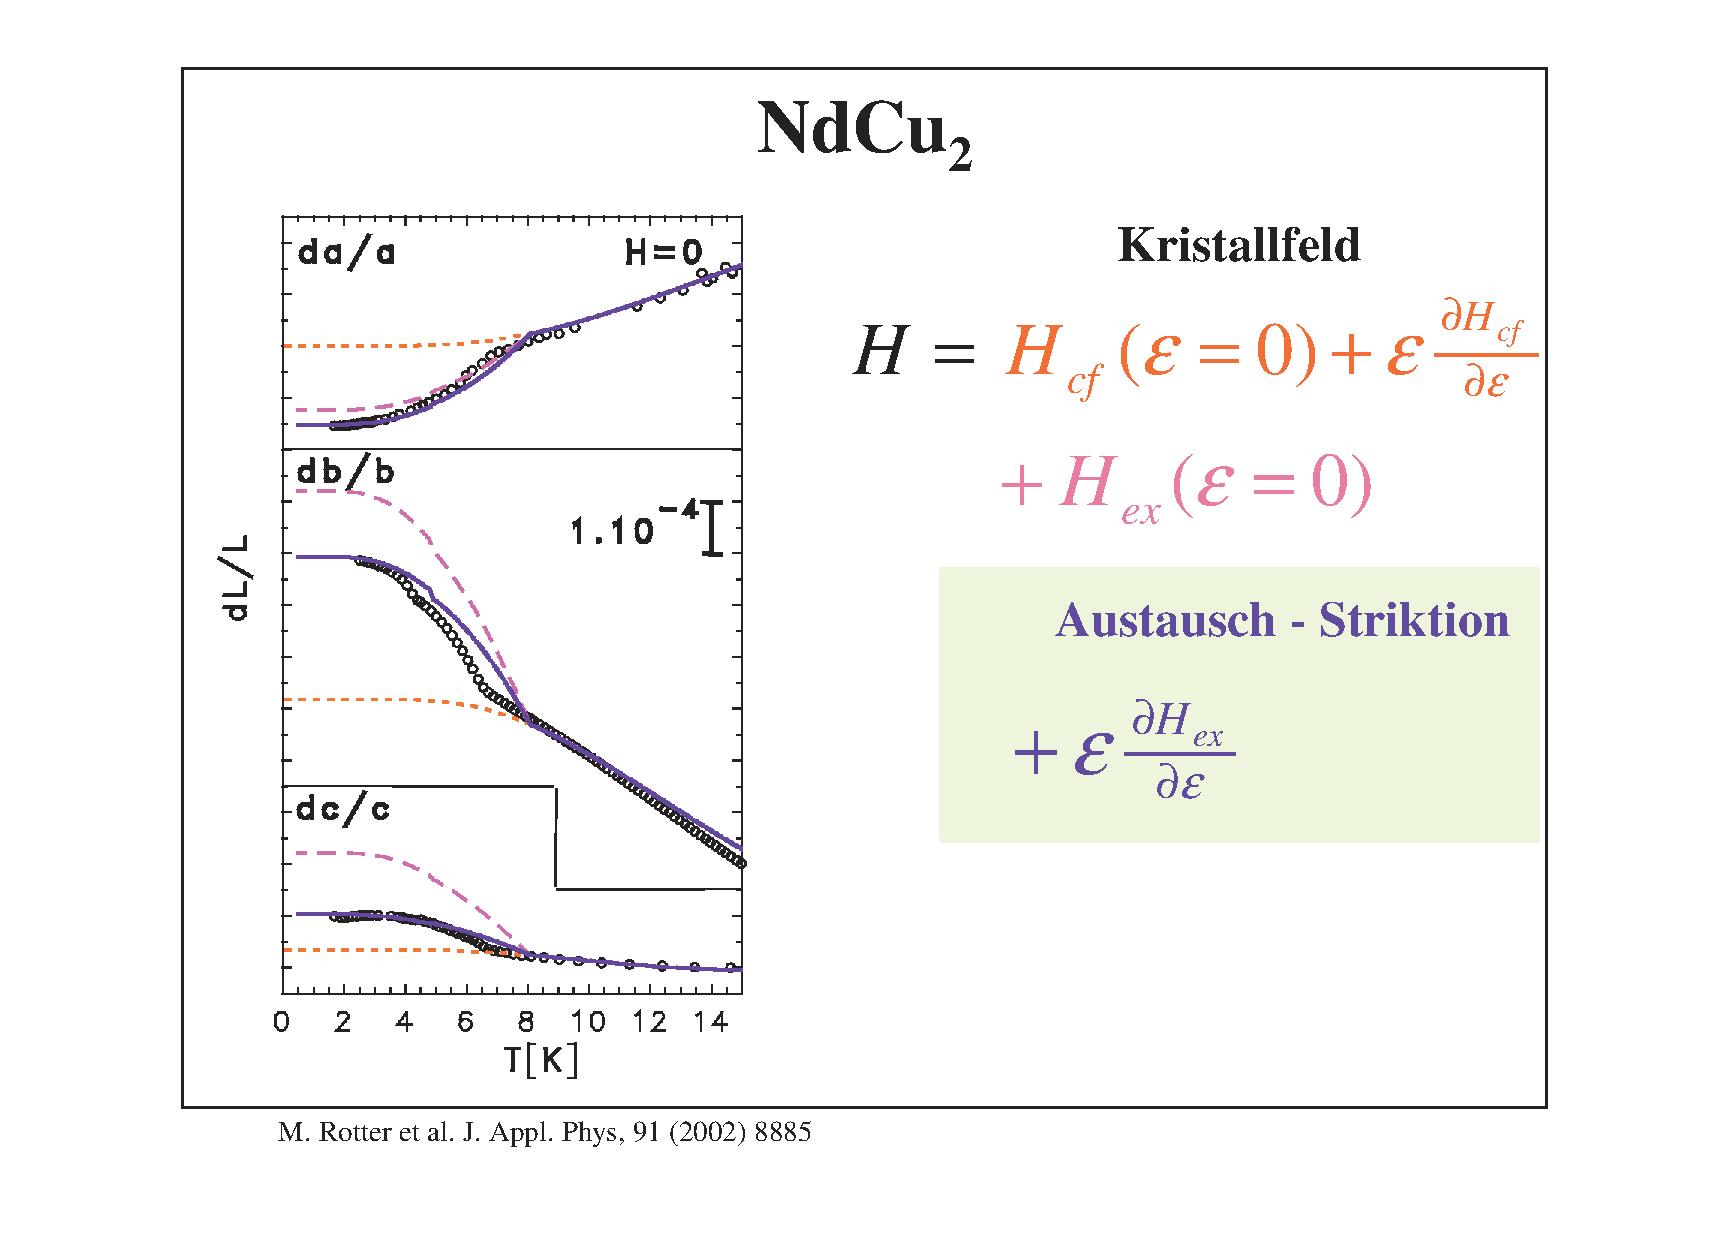
\includegraphics[angle=0, width=0.8\textwidth]{figsrc/magnetostriction_ndcu2.eps}
\end{center}
\caption{Calculated spontaneous magnetostriction of NdCu$_2$.}
\label{magnetostrictiongraphic}
\end{figure}

\begin{description}
\item [\prg mcphas.qvc]    the set of test q-vectors used for calculation of free energy.
                           Components of these q vectors refer to the reciprocal lattice $\vec a^*,\vec b^*,\vec c^*$.
\item [\prg mcphas.phs]    spin-configuration table of different types of spin-configurations. 
                            Note, in case of non-orthogonal axes the convention in these tables 
                            is $mb||\vec b$, $mc||(\vec a \times \vec b)$ and $ma$ perpendicular to $mb$ and $mc$.

                           {\em Note}: 
                           there is no natural criteria for deciding, if one spin-configuration is
			   different from another one. Therefore the list of ''different''
			   spin-configurations is dependent on the meaning of ''different''.
			   
			   The program {\prg McPhase} decides whether a spin-configuration is
			   different from another by a simple criteria, namely by the
			   angle between the spins. Comparing two spin configurations it calculates
			   the angle between corresponding spins and if for one spin the
			   angle is not small, the configuration is treated as a different
			   configuration. Therefore for example a ferromagnet with moments
			   in $a$ has a different spin configuration than a ferromagnet with
			   moments in $b$ direction. 
\item [\prg mcphas.sps]    $T-H$ dependence of spin-configuration. The spin configurations stored in this
                           file may be displayed using the program {\prg spins\index{spins}}, an example is given
			   in figure~\ref{spingraphic}.
                            Note, in case of non-orthogonal axes the convention for applied field $Ha, Hb,Hc$ and
                            also for the moment components $ma, mb, mc$ in these tables 
                            is $mb||\vec b$, $mc||(\vec a \times \vec b)$ and $ma$ perpendicular to $mb$ and $mc$.

\item [\prg mcphas.mf]     $T-H$ dependence of exchange field configuration, stored as $g_J \mu_B H_{xc}(i)$(unit is in meV)
                            for i=1,2,...,number of spins in magnetic unit cell.
                            Note, in case of non-orthogonal axes the convention for applied field $Ha, Hb,Hc$ and
                            also for the mean field components in these tables 
                            is $Hb||\vec b$, $Hc||(\vec a \times \vec b)$ and $Ha$ perpendicular to $Hb$ and $Hc$.
\item [\prg mcphas.fum]    free energy, magnetic energy (the derivative with respect to temperature gives the specific %%@
heat),
                           magnetisation data and (if cfield is used with higher order interactions)
                           expectation values of the Stevens Operators $<O_l^m>$ . As an example for the information
			   contained in this file the calculated magnetisation and magnetostriction of NdCu$_2$ is shown in
			   figures~\ref{magnetization} and ~\ref{magnetizationgraphic}.
                            Note, in case of non-orthogonal axes the convention for applied field $Ha, Hb,Hc$ and
                            also for the magnetisation components $ma,mb,mc$ in these tables 
                            is $Hb||\vec b$, $Hc||(\vec a \times \vec b)$ and $Ha$ perpendicular to $Hb$ and $Hc$.

\item [\prg mcphas1.j1 .j1 .j2 ...] 
               spin-spin correlation functions for sub-lattice 1 neighbour 1 2 ...
	       (linear combination is proportional to magnetostriction)
	       The spin-spin correlation functions for neighbour $k$ are defined by
	       the following sum of dyadic products:

	       \begin{equation}
	        \frac{1}{n}\sum_{s=1}^n <{\mbf J}^s> \times  <{\mbf J}^{s+k}>
	       \end{equation}
	       with $n$ being the number of moments in the magnetic unit cell.
	       Single ion and two-ion magnetostriction can be calculated using the $<O_l^m>$ and the
	       spin-spin correlation functions. As an example the magnetostriction analysis of
	       NdCu$_2$ is shown in figure~\ref{magnetostrictiongraphic}. For details 
             please refer to~\cite{rotter02-8885}.
                            Note, in case of non-orthogonal axes the convention for applied field $Ha, Hb,Hc$ and
                            also for the moment components in these tables 
                            is $Hb||\vec b$, $Hc||(\vec a \times \vec b)$ and $Ha$ perpendicular to $Hb$ and $Hc$.
\item [\prg mcphas.xyt]    phase diagram as x,y,T, H, phase-number j according to spin-configuration table
               given in mcphas.phs, a periodicity key, nettomoments <J>.
 Figure~\ref{phasediagramgraphic}
	       shows the phase diagram of NdCu$_2$ for magnetic fields parallel to the orthorhombic $b$-direction.
                            Note, in case of non-orthogonal axes the convention for applied field $Ha, Hb,Hc$ 
                             in these tables 
                            is $Hb||\vec b$, $Hc||(\vec a \times \vec b)$ and $Ha$ perpendicular to $Hb$ and $Hc$.
\item [\prg mcphas.hkl]    calculated (unpolarised) neutron diffraction data (the calculated magnetic intensities
    correspond to the magnetic structure + Polarisation factor. The
    Lorentz-factor , magnetic form factor and  instrumental corrections are not calculated.)
 As an example figure~\ref{neutintgraphic}
    shows the calculated temperature dependence of magnetic amplitudes for NdCu$_2$.
                           $h,k,l$ refer to the reciprocal lattice $\vec a^*,\vec b^*,\vec c^*$.
                            Note, in case of non-orthogonal axes the convention for applied field $Ha, Hb,Hc$ 
                             in these tables 
                            is $Hb||\vec b$, $Hc||(\vec a \times \vec b)$ and $Ha$ perpendicular to $Hb$ and $Hc$.
    
\item [\prg mcphasa.hkl]    Fourier Transform of the $a$-component of the magnetic Moments.
                           $h,k,l$ refer to the reciprocal lattice $\vec a^*,\vec b^*,\vec c^*$.
                            Note, in case of non-orthogonal axes the convention for applied field $Ha, Hb,Hc$ and
                            the magnetic moment component in these tables 
                            is $Hb||\vec b$, $Hc||(\vec a \times \vec b)$ and $Ha$ perpendicular to $Hb$ and $Hc$.
\item [\prg mcphasb.hkl]    Fourier Transform of the $b$-component of the magnetic Moments.
                           $h,k,l$ refer to the reciprocal lattice $\vec a^*,\vec b^*,\vec c^*$.
                            Note, in case of non-orthogonal axes the convention for applied field $Ha, Hb,Hc$ and
                            the magnetic moment component in these tables 
                            is $Hb||\vec b$, $Hc||(\vec a \times \vec b)$ and $Ha$ perpendicular to $Hb$ and $Hc$.
\item [\prg mcphasc.hkl]    Fourier Transform of the $c$-component of the magnetic Moments.
                           $h,k,l$ refer to the reciprocal lattice $\vec a^*,\vec b^*,\vec c^*$.
                            Note, in case of non-orthogonal axes the convention for applied field $Ha, Hb,Hc$ and
                            the magnetic moment component in these tables 
                            is $Hb||\vec b$, $Hc||(\vec a \times \vec b)$ and $Ha$ perpendicular to $Hb$ and $Hc$.
\end{description} 

\vspace{1cm}
{\em Exercises:}
\begin{itemize}
\item Look at the output files of {\prg McPhase}  in the directory
{\prg examples/ndcu2b\_new/results}.  At which magnetic field
the ferromagnetically aligned state is achieved (at $T=$2~K)?
\item
What is the propagation vector in the different antiferromagnetic phases at $T=$2~K ?
\end{itemize}





\subsubsection{{\prg mcphas.j\index{mcphas.j}} - lattice and exchange parameters}\label{mcphasj}
This file provides the information about 
the crystallographic
 structure and the magnetic exchange interactions.
For every atom in the crystallographic basis there
has to be given the coordinates, the number of neighbours to be considered, the 
Land\'e factor $g_J$, the single ion property filename and  a set of exchange parameters.
If the exchange parameters (and neighbour positions) are not known for your system, you 
can use the program module {\prg makenn\index{makenn}} (see section \ref{addprog}) to generate 
a list of nearest neighbours and
exchange parameters, currently implemented in {\prg makenn\index{makenn}} are dipolar interactions,
exchange interactions via the Bethe-Slater curve or the RKKY model. Note that in order
to use {\prg makenn\index{makenn}} you have to set up a working {\prg mcphas.j\index{mcphas.j}} file, which may or
may not contain neighbours and interactions.

Use program {\prg addj\index{addj}} to add exchange parameter set stored in different 
such {\prg .j} files (see section~\ref{addprog}).



\begin{description}
\item [Line 1,2:] Comment Lines
\item [Line 3:] lattice constants a,b,c and crystal angles alpha, beta, gamma 
\item [Line 4-6:] primitive lattice vectors
\item [Line 7:] Number of atoms in the primitive crystallographic unit cell ({\prg nofatoms})
\item [Line 8:] a comment line with stars
\item [Line 9:] coordinates  ($d_a$,$d_b$,$d_c$) of 1$^{st}$ magnetic ion in the crystallographic unit cell  with
respect to the lattice vectors $\vec a$,$\vec b$,$\vec c$. The number of neighbours of this 
ion, for which interaction constants are given in the interaction table (nofneighbours). 
If {\prg diagonalexchange}
is set to 0 the 9 components of the exchange tensor are given in column 4-12. 
If {\prg diagonalexchange}
 is 1, only 3 components are given (column 4-6).
If {\prg diagonalexchange}
 is 2, specific components of the exchange tensor can be given in columns 4 onwards. The indices of these components
 must be given in the following line (Line 9a below).
The Land\'e factor of the ion (gJ) and the file name of the corresponding single ion
parameter file (cffilename).
\item [Line 9a:]  If {\prg diagonalexchange=2}, then this line gives the indices of the exchange tensor corresponding to 
 the columns 4 onwards. It must have a variable called {\prg indexexchange} followed by a list of names of components of the interaction
 tensor separated by space. E.g.
 \verb|  #! indexexchange= JaJb JbJc  | 
means column 4 gives the the interaction constant between the
 first angular momentum component of the current ion with the second angular momentum component of its neighbour, whilst 
 column 5 has the interaction constant between the second angular momentum component of this ion with the third component of its
 neighbour. Alternatively, pairs of numbers may be given, as in \verb|  #! indexexchange= 1,2 2,3  |
 Additionally another parameter {\prg symmetricexchange} can be set to 1, where the value in each column is also used 
 for the transposed tensor component. Thus \verb|  #! symmetricexchange=1 indexexchange= JaJb  | is the same as \\
 \verb|  #! indexexchange= JaJb JbJa  | where the 4th and 5th column are the same.
\item [Line 10:]  Comment line
\item [Line 11-(10+nofneighbours):] Interaction table for ion number 1.   
Note: the neighbour coordinates (column 1-3) are given with respect to the lattice vectors
$\vec a$,$\vec b$,$\vec c$. The program then calculates from these values the coordinates
with respect to the primitive lattice $\vec r_1$,~$\vec r_2$,~$\vec r_3$.
($ d_a \vec a + d_b \vec b + d_c \vec c = d_1 \vec r_1 + d_2 \vec r_2 + d_3 \vec r_3$).
Column 4,5,6 \dots contain the components of the interaction tensor $\stackrel{=}{\mathcal J}$. 
Note that in case of non-orthogonal axes the 
components of the moments and the interaction tensor $Ja, Jb, Jc, Jaa, Jbb, Jcc, Jab ...$ 
refer to the orthogonal coordinate system
defined with respect to the nonorthogonal lattice $\vec a,\vec b,\vec c$ as
$Jb||\vec b$, $Jc||(\vec a \times \vec b)$ and $Ja$ perpendicular to $Jb$ and $Jc$.
\item [Line (11+nofneighbours) - end:] for each ion in the unit cell line 8 - (10+nofneighbours)
are repeated.
\end{description}


\vspace{0.5cm}

{\small {\bf Information for experienced users:}
\begin{description}
\item[\prg mcphas.jjj:]
format of exchange parameter file, which only needs a reduced set of exchange
parameters in the input file. Using the program {\prg jjj2j} the file can be transformed
to {\prg mcphas.j\index{mcphas.j}} by adding lines for all the equivalent neighbours. The format definition
of {\prg mcphas.jjj} is the same as {\prg mcphas.j\index{mcphas.j}}, however each line denotes several
equivalent neighbour atoms (instead of only one in {\prg mcphas.j\index{mcphas.j}}) according to the
 following rules:
\begin{itemize}
\item If a nonzero coordinate $d_a$ (or $d_b$,$d_c$) in the interaction table
 corresponds to it's value at the nearest
 lattice point of the primitive lattice,
  additional interactions of the same size
with  neighbours with coordinate $-d_a$ (or $-d_b$,$-d_c$, respectively)
are taken into account. This
holds for each of the three coordinates $d_a$,$d_b$ and $d_c$
 resulting in a maximum
number of 8 equivalent neighbours per line in the interaction table.
\item If the value of $d_a$ (or $d_b$,$d_c$) is zero or differs
from it's value at the nearest lattice point of the primitive lattice, it is 
changed to the value at the nearest lattice point and {\bf no} interaction 
with  neighbours with coordinates $-d_a$ (or $-d_b$,$-d_c$) is
 taken into account. If such
 interaction is needed it may be given in a different line and may
have different magnitude. In this way also crystallographic lattices
with no mirror symmetry may be described.
\end{itemize}
\item[\prg mcphas.coq:]   exchange parameters etc [ in old format]...see examples for details, use {\prg coq2jjj} to 
transform {\prg mcphas.coq} to {\prg mcphas.jjj} format
\end{description}

}


\subsubsection{Example {\prg mcphas.j\index{mcphas.j}} file for a simple antiferromagnet}

Here are example files of a tetragonal antiferromagnet with nearest neighbour interactions, all
files are equivalent:

{\small
\begin{verbatim} 
# simple antiferromagnet 
#<!--mcphase.mcphas.j-->
#***************************************************************
# Lattice Constants (A)
#! a=4.3843 b=4.3843 c=2.4194 alpha=  90 beta=  90 gamma=  90
#! r1a=   1 r2a=   0 r3a=   0
#! r1b=   0 r2b=   1 r3b=   0   primitive lattice vectors [a][b][c]
#! r1c=   0 r2c=   0 r3c=   1
#! nofatoms=1  nofcomponents=3  number of atoms in primitive unit cell/number of components of each spin
# ****************************************************************************
#! da=  0 [a] db=  0 [b] dc=  0 nofneighbours=2 diagonalexchange=0 gJ=0.857143 cffilename=Ce3p.sipf
# da[a] db[b] dc[c] Jaa[meV] Jbb[meV] Jcc[meV] Jab[meV] Jba[meV] Jac[meV] Jca[meV] Jbc[meV] Jcb[meV]
+0	+0	+1	-0.1	-0.1	-0.1   0  0  0  0  0  0
+0	+0	-1	-0.1	-0.1	-0.1   0  0  0  0  0  0
#\end{verbatim}
}

Using diagonalexchange this may be shortened to

{\small
\begin{verbatim} 
# simple antiferromagnet 
#<!--mcphase.mcphas.j-->
#***************************************************************
# Lattice Constants (A)
#! a=4.3843 b=4.3843 c=2.4194 alpha=  90 beta=  90 gamma=  90
#! r1a=   1 r2a=   0 r3a=   0
#! r1b=   0 r2b=   1 r3b=   0   primitive lattice vectors [a][b][c]
#! r1c=   0 r2c=   0 r3c=   1
#! nofatoms=1  nofcomponents=3  number of atoms in primitive unit cell/number of components of each spin
# ****************************************************************************
#! da=  0 [a] db=  0 [b] dc=  0 nofneighbours=2 diagonalexchange=1 gJ=0.857143 cffilename=Ce3p.sipf
# da[a] db[b] dc[c] Jaa[meV] Jbb[meV] Jcc[meV] Jab[meV] Jba[meV] Jac[meV] Jca[meV] Jbc[meV] Jcb[meV]
+0	+0	+1	-0.1	-0.1	-0.1   
+0	+0	-1	-0.1	-0.1	-0.1   
#\end{verbatim}
}

with indexexchange option the sequence of two ion interaction parameters can be changed and
zero parameters may be omitted:

{\small
\begin{verbatim} 
# simple antiferromagnet 
#<!--mcphase.mcphas.j-->
#***************************************************************
# Lattice Constants (A)
#! a=4.3843 b=4.3843 c=2.4194 alpha=  90 beta=  90 gamma=  90
#! r1a=   1 r2a=   0 r3a=   0
#! r1b=   0 r2b=   1 r3b=   0   primitive lattice vectors [a][b][c]
#! r1c=   0 r2c=   0 r3c=   1
#! nofatoms=1  nofcomponents=3  number of atoms in primitive unit cell/number of components of each spin
# ****************************************************************************
#! da=  0 [a] db=  0 [b] dc=  0 nofneighbours=2 diagonalexchange=2 gJ=0.857143 cffilename=Ce3p.sipf
# da[a] db[b] dc[c] Jaa[meV] Jbb[meV] Jcc[meV] Jab[meV] Jba[meV] Jac[meV] Jca[meV] Jbc[meV] Jcb[meV]
#! indexexchange = JaJa JaJc JcJa JbJb JcJc
+0	+0	+1	-0.1 0 0 -0.1	-0.1  
+0	+0	-1	-0.1 0 0 -0.1	-0.1  
#\end{verbatim}
}

{\small
\begin{verbatim} 
# simple antiferromagnet 
#<!--mcphase.mcphas.j-->
#***************************************************************
# Lattice Constants (A)
#! a=4.3843 b=4.3843 c=2.4194 alpha=  90 beta=  90 gamma=  90
#! r1a=   1 r2a=   0 r3a=   0
#! r1b=   0 r2b=   1 r3b=   0   primitive lattice vectors [a][b][c]
#! r1c=   0 r2c=   0 r3c=   1
#! nofatoms=1  nofcomponents=3  number of atoms in primitive unit cell/number of components of each spin
# ****************************************************************************
#! da=  0 [a] db=  0 [b] dc=  0 nofneighbours=2 diagonalexchange=2 gJ=0.857143 cffilename=Ce3p.sipf
# da[a] db[b] dc[c] Jaa[meV] Jbb[meV] Jcc[meV] Jab[meV] Jba[meV] Jac[meV] Jca[meV] Jbc[meV] Jcb[meV]
#! indexexchange = 1,1 1,3, 3,1 2,2 3,3
+0	+0	+1	-0.1 0 0 -0.1	-0.1  
+0	+0	-1	-0.1 0 0 -0.1	-0.1  
#\end{verbatim}
}


using symmetricexchange together with indexexchange will assume that the interaction tensor is symmetic and 
only half of it may be given:

{\small
\begin{verbatim} 
# simple antiferromagnet 
#<!--mcphase.mcphas.j-->
#***************************************************************
# Lattice Constants (A)
#! a=4.3843 b=4.3843 c=2.4194 alpha=  90 beta=  90 gamma=  90
#! r1a=   1 r2a=   0 r3a=   0
#! r1b=   0 r2b=   1 r3b=   0   primitive lattice vectors [a][b][c]
#! r1c=   0 r2c=   0 r3c=   1
#! nofatoms=1  nofcomponents=3  number of atoms in primitive unit cell/number of components of each spin
# ****************************************************************************
#! da=  0 [a] db=  0 [b] dc=  0 nofneighbours=2 diagonalexchange=2 gJ=0.857143 cffilename=Ce3p.sipf
# da[a] db[b] dc[c] Jaa[meV] Jbb[meV] Jcc[meV] Jab[meV] Jba[meV] Jac[meV] Jca[meV] Jbc[meV] Jcb[meV]
#! symmetricexchange=1 indexexchange = JaJa JaJc JbJb JcJc
+0	+0	+1	-0.1 0  -0.1	-0.1  
+0	+0	-1	-0.1 0  -0.1	-0.1  
#\end{verbatim}
}


\subsubsection{Single Ion Property Input Files}\label{sifile}

In order to speed up calculations or treat special problems a large 
variety of single ion modules is available. This includes the
option to load a user written single ion module. Details are 
given in chapter~\ref{simod}.

The first time user of {\prg McPhase} should use the module {\prg so1ion}\index{so1ion} and 
create an appropriate single ion property input file as described in
section \ref{cf1ion}. A good starting point are several examples
given in directory {\prg examples}.


\subsubsection{Example single ion property file  for a simple antiferromagnet}

Here is an example file {\prg mcphas.cf1} describing the anisotropy of a 
simple antiferromagnet with Ce atoms having basal plane anisotropy. Note the
axis convention xyz$||$abc, in case of non-orthogonal axes the convention 
is $y||\vec b$, $z||(\vec a \times \vec b)$ and $x$ perpendicular to $y$ and $z$.


\section{{\prg mcphas} - calculation of thermodynamic properties (Magnetisation, Susceptibility, Specific Heat, Neutron %%@
Diffraction, etc.)}
\label{runmcphas}

In order to perform calculations beyond the capabilities of {\prg cfield\index{cfield}} it is necessary
to use the program {\prg mcphas}. 
\begin{itemize}
\item As a first step it is possible to
calculate the thermodynamic properties such as magnetisation or specific heat
considering only single ion effects. In this case all the exchange parameters
have to be set to zero in {\prg mcphas.j\index{mcphas.j}}. 
\item for more advanced calculations the two - ion interactions have to be
considered and may lead to magnetic order. {\prg mcphas} can perform 
calculations in the ordered state in the following way: for 
a given temperature $T$ and magnetic field $\mbf H$ (vector)
several possible magnetic structures are stabilised
by a mean field algorithm and the free energy is 
calculated. The initial values for this mean-field procedure are
modified by a Monte Carlo process.


The temperature and magnetic field is varied during the calculation
and thereby it is possible to map out the magnetic phase diagram.
\end{itemize}

The program produces a plot of the stabilised magnetic
structures and the magnetisation on screen, the
output files contain additional information 
such as calculated magnetoelastic and  neutron-scattering
data. Several graphic programs easy the visualisation of the
calculated data (section~\ref{graphics}).



\subsection{Input Files}
The program {\prg McPhase} needs the following input files (all in the same directory)
 in order to run:

\begin{enumerate}
\item {\prg mcphas.ini\index{mcphas.ini}}
 - controlling the algorithm
\item {\prg mcphas.j\index{mcphas.j}}
  - lattice and exchange parameters
\item {\prg mcphas.tst\index{mcphas.tst}(optional)}  - test spin configurations
\item {\prg single-ion property files}
\item {\prg directory ./results/}
 - directory where calculated data is stored
\item {\prg directory ./fit} - experimental data for fit (optional)
\end{enumerate}


 All
 of these input files have to be in one directory and the program
has to be started in this directory. The results of the simulation
are then stored in the  subdirectory ./results/, which must exist before starting
the program 
... see directory ./examples/ for some examples.
 In order to prepare these files
for a new calculation it is best to take them from an example, copy the files
to a new directory and make the
modifications  to adapt them to the new problem.

\subsubsection{Example - a simple antiferromagnet}

In the following description of the input files we will always refer
to a simple example: a simple antiferromagnet
on a primitive orthorhombic lattice. The first time user
will thus have a simple example to follow, all corresponding
files are given in the directory {\prg tutorial/03magnetic\_phases\_mcphas/simpleAF}.
 

\subsubsection{{\prg mcphas.ini\index{mcphas.ini}} - controlling the algorithm}
   Initial file containing algorithm control parameters, for instance the range and spacing of
   propagation vectors Q or the number of Monte Carlo trials for initial spin configurations
    - {\em mind}: this
   file is rewritten and reread  when running the program and may be changed by the
   user in order to manipulate the running simulation.

{\prg mcphas.ini\index{mcphas.ini}} consists of several sections:
\begin{description}
\item [MCPHASE RUNTIME CONTROL:] this section contains the parameters
controlling the status of the calculation.
\item [XY PHASEDIAGRAM PARAMETERS:] here the temperature and field range and
step widths of the calculation are specified.
The definition of the x and y
axis in terms of temperature and magnetic field is followed by the
corresponding range and step width. An offset may be given for all
field and temperature values.
Note that for most cases of interest
this offset is zero (T0=0, Ha0=0, Hb0=0, Hc0=0).
 For the simple case of calculating a Temperature-Field phase diagram
 It is just necessary to set xT=1 and give the temperature range by
xmin/xmax/xstep. For field in b direction then just set yHb=1 and 
define the range in ymin/ymax/ystep.
In case of non-orthogonal axes the applied magnetic field
components $Ha, Hb, Hc$ refer to the orthogonal coordinate system
defined with respect to the nonorthogonal lattice $\mbf a,\mbf b,\mbf c$ as
$Hb||\mbf b$, $Hc||(\mbf a \times \mbf b)$ and $Ha$ perpendicular to $Hb$ and $Hc$.

\item [GENERATION OF SPINCONFIGURATIONS:] at the beginning of the program
some initial values of spin configurations are generated from a set of 
propagation vectors. This section defines the range of propagation vectors
and the step width.
Depending on the value of the propagation Q with respect to the primitive reciprocal lattice
1-, 2- or 3-dimensional simulations of magnetic lattices
are possible. It is advisable to 
think carefully about the chosen range and spacing of Q vectors in order
to limit calculation time.
 
For example a good starting point is to begin with a calculation with large
step widths (e.g. 0.1)  covering the Brillouin zone. This should give an idea
of the propagation vectors which are stabilised. An advanced calculation
could then fine tune the propagation and determine its accurate value (using
small step widths in a limited area of the zone).
The verbose option of {\prg mcphas} allows to inspect the propagation vectors
which are actually used in the calculation.
Trick: in order to get a quick overview of the
q-vector range covered by the mcphas\index{mcphas} simulation start mcphas, exit and 
just type {\prg felog ./results/mcphas.qvc} (need {\prg perl,perldl,pdl,pgplot} packages).

In order to limit calculation time, the maximum periodicity
of the magnetic unit cell with respect to the crystallographic unit cell 
(maxqperiod) and the maximum number of spins in the magnetic unit cell 
(maxnofspins) can be limited. Also the maximum number of test spin configurations
in the internal table can be limited (maxnoftestspincf).
A critical feature with respect to calculation time is also the number of
spin configurations which are generated by a random process from a tabulated
SPINCONFIGURATIONS during the calculation. 

In summary the variables in this section are mainly important to adapt the
program to a given computer system with finite speed. They have to be set
to optimise between speed and accuracy of the calculation. In order to
find appropriate values it is best to perform some calculations 
and restrict the parameters step by step if insufficient speed is obtained.
Also the examples included in the program package may serve as starting
points.

\item [PARAMETERS FOR SUB FECALC SELFCONSISTENCY PROCESS:] the most important
procedure in the module {\prg mcphas} is the sub fecalc. In this part of the 
program the self consistent calculation of the magnetic moment configuration
is performed as shown schematically in fig.~\ref{fecalc}. 
In the mean field approximation the Hamiltonian~(\ref{hamilton}) is approximated
by

\begin{equation}
 {\mathcal H}=\sum_n H_{SI}^n + E_{corr}
\end{equation}

with the single ion Hamiltonian (in case of module {\prg so1ion\index{so1ion}})

\begin{equation}
H_{SI}^n=  B_l^m O_{lm}({\mbf J}^n) 
	     - g_{Jn} \mu_B {\mbf J}^n {\mbf H^n_{eff}} 
\end{equation}

and the correction term

\begin{equation}
E_{corr}=\frac{1}{2}\sum_{n} g_{Jn} \mu_B \langle {\mbf J}^n
 \rangle (\mbf H^n_{eff}-\mbf H) 
\end{equation}

and with the mean fields $ \mbf H^n_{eff}$ given by

\begin{equation}\label{meanfield}
\mbf H^n_{eff}=\mbf H + \mbf H^n_{xc}=\mbf H+\sum_{{\mbf G'}n'} \frac{{\mathcal J}
(\mbf r_n-(\mbf G'+\mbf r_{n'}))}{g_{Jn}\mu_B } \langle{\mbf
J}^{n'}\rangle
\end{equation}

These mean fields and the moments $\langle \mbf J^n \rangle$ 
are determined in a self consistent
way. For a given magnetic unit cell and initial configuration 
of magnetic moments
the mean fields are calculated according to equation~(\ref{meanfield}). 
Then, for each
magnetic ion the single ion property module is taken 
and the magnetic moment $\langle \mbf J^n \rangle$ is 
calculated from it's mean field. The mean fields are used again in equation~(\ref{meanfield})
and so on .... until convergence is reached. 
Then, the free energy ($f=-kT\sum_n \ln(z_n) + E_{corr}$ ) 
of the stabilised
configuration is calculated (this is why this sub is called {\prg fecalc}). 
The free energies of a lot of different stabilised configurations have to
be compared in order to find out which configuration has lowest free energy, i.e.
is stable in thermal  equilibrium.

It may happen that this process does
not converge due to bad choice of the initial configuration, therefore a maximum number
of mean field loops has to be given by the user.
The results of a calculation may be significantly influenced by
changing parameters such as the maximum number of iteration loops 
in this section. 
In fact the simulation is always a compromise of calculation time and accuracy: if only
a few initial spin configurations are tried at each (H-T) point, the calculation speed is
fast, however it is possible that the program misses the magnetic structure with the
lowest free energy. The same holds if other critical parameters of the simulation are
restricted too much.
 

\item [OUTPUT OF PHYSICAL PROPERTIES:]
Some options for the output of the calculation can be changed in this section.
\end{description}

\begin{figure}[hb]
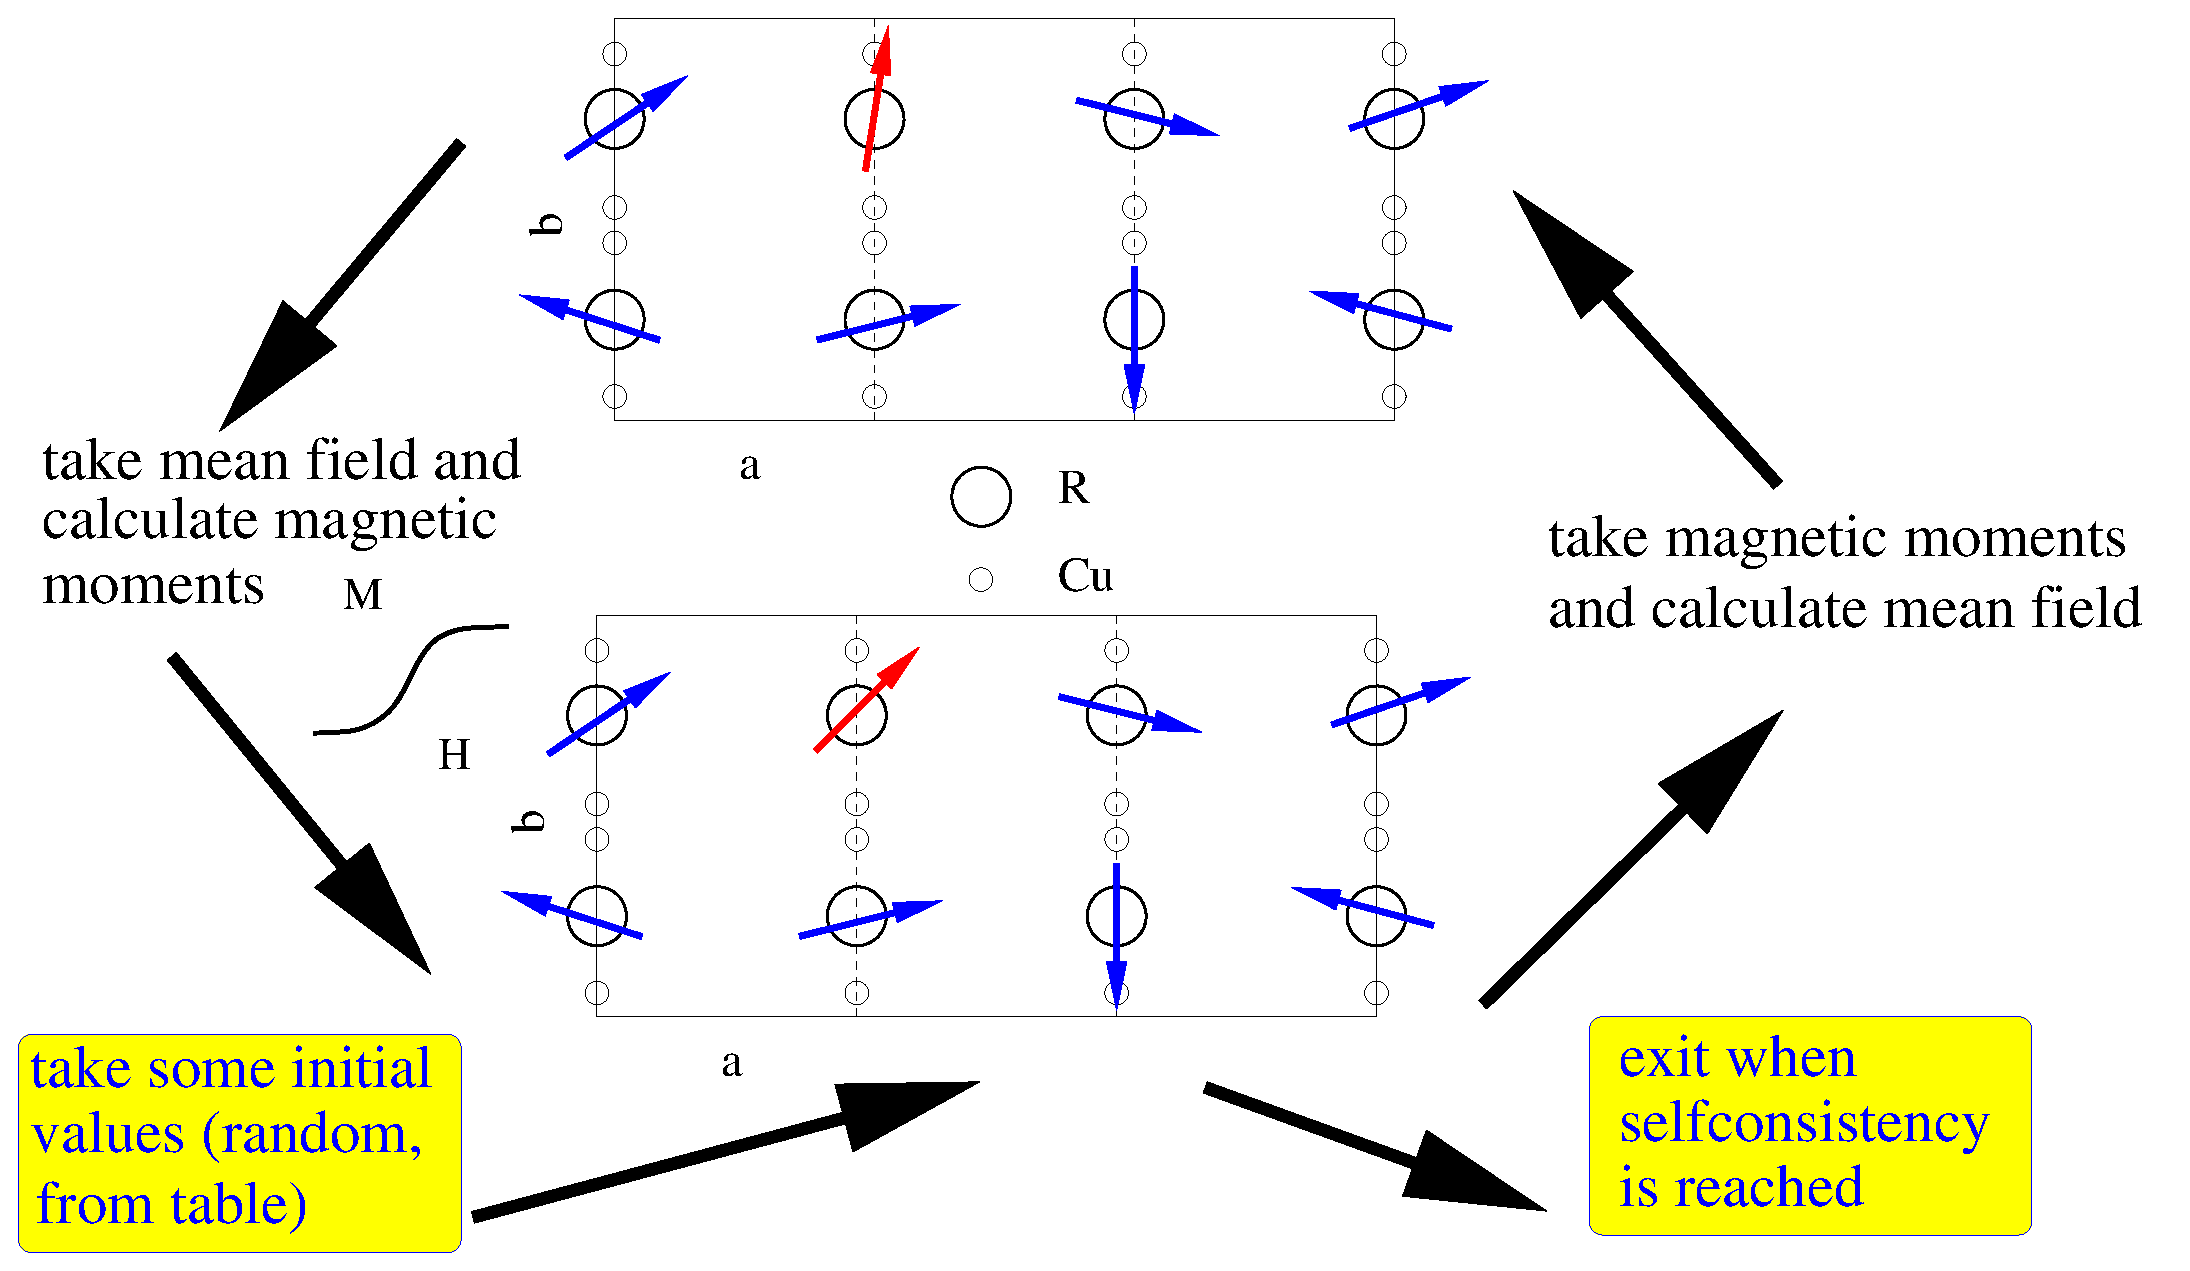
\includegraphics[angle=0,width=0.9\columnwidth]{figsrc/fecalc.eps}
\caption{\label{fecalc}Mean field process of sub {\prg fecalc}.}
\end{figure}

 
\subsubsection{Example {\prg mcphas.ini\index{mcphas.ini}} file for a simple antiferromagnet}

Here is an example of {\prg mcphas.ini\index{mcphas.ini}}, the comments describe the meaning of the different
parameters:

\input{mcphas.ini}



\subsubsection{{\prg mcphas.j\index{mcphas.j}} - lattice and exchange parameters}\label{mcphasj}
This file provides the information about 
the crystallographic
 structure and the magnetic exchange interactions.
For every atom in the crystallographic basis there
has to be given the coordinates, the number of neighbours to be considered, the 
Land\'e factor $g_J$, the single ion property filename and  a set of exchange parameters.
If the exchange parameters (and neighbour positions) are not known for your system, you 
can use the program module {\prg makenn\index{makenn}} (see section \ref{addprog}) to generate 
a list of nearest neighbours and
exchange parameters, currently implemented in {\prg makenn\index{makenn}} are dipolar interactions,
exchange interactions via the Bethe-Slater curve or the RKKY model. Note that in order
to use {\prg makenn\index{makenn}} you have to set up a working {\prg mcphas.j\index{mcphas.j}} file, which may or
may not contain neighbours and interactions.

Use program {\prg addj\index{addj}} to add exchange parameter set stored in different 
such {\prg .j} files (see section~\ref{addprog}).



\begin{description}
\item [Line 1,2:] Comment Lines
\item [Line 3:] lattice constants a,b,c and crystal angles alpha, beta, gamma 
\item [Line 4-6:] primitive lattice vectors
\item [Line 7:] Number of atoms in the primitive crystallographic unit cell ({\prg nofatoms})
\item [Line 8:] a comment line with stars
\item [Line 9:] coordinates  ($d_a$,$d_b$,$d_c$) of 1$^{st}$ magnetic ion in the crystallographic unit cell  with
respect to the lattice vectors $\vec a$,$\vec b$,$\vec c$. The number of neighbours of this 
ion, for which interaction constants are given in the interaction table (nofneighbours). 
If {\prg diagonalexchange}
is set to 0 the 9 components of the exchange tensor are given in column 4-12. 
If {\prg diagonalexchange}
 is 1, only 3 components are given (column 4-6).
If {\prg diagonalexchange}
 is 2, specific components of the exchange tensor can be given in columns 4 onwards. The indices of these components
 must be given in the following line (Line 9a below).
The Land\'e factor of the ion (gJ) and the file name of the corresponding single ion
parameter file (cffilename).
\item [Line 9a:]  If {\prg diagonalexchange=2}, then this line gives the indices of the exchange tensor corresponding to 
 the columns 4 onwards. It must have a variable called {\prg indexexchange} followed by a list of names of components of the interaction
 tensor separated by space. E.g.
 \verb|  #! indexexchange= JaJb JbJc  | 
means column 4 gives the the interaction constant between the
 first angular momentum component of the current ion with the second angular momentum component of its neighbour, whilst 
 column 5 has the interaction constant between the second angular momentum component of this ion with the third component of its
 neighbour. Alternatively, pairs of numbers may be given, as in \verb|  #! indexexchange= 1,2 2,3  |
 Additionally another parameter {\prg symmetricexchange} can be set to 1, where the value in each column is also used 
 for the transposed tensor component. Thus \verb|  #! symmetricexchange=1 indexexchange= JaJb  | is the same as \\
 \verb|  #! indexexchange= JaJb JbJa  | where the 4th and 5th column are the same.
\item [Line 10:]  Comment line
\item [Line 11-(10+nofneighbours):] Interaction table for ion number 1.   
Note: the neighbour coordinates (column 1-3) are given with respect to the lattice vectors
$\vec a$,$\vec b$,$\vec c$. The program then calculates from these values the coordinates
with respect to the primitive lattice $\vec r_1$,~$\vec r_2$,~$\vec r_3$.
($ d_a \vec a + d_b \vec b + d_c \vec c = d_1 \vec r_1 + d_2 \vec r_2 + d_3 \vec r_3$).
Column 4,5,6 \dots contain the components of the interaction tensor $\stackrel{=}{\mathcal J}$. 
Note that in case of non-orthogonal axes the 
components of the moments and the interaction tensor $Ja, Jb, Jc, Jaa, Jbb, Jcc, Jab ...$ 
refer to the orthogonal coordinate system
defined with respect to the nonorthogonal lattice $\vec a,\vec b,\vec c$ as
$Jb||\vec b$, $Jc||(\vec a \times \vec b)$ and $Ja$ perpendicular to $Jb$ and $Jc$.
\item [Line (11+nofneighbours) - end:] for each ion in the unit cell line 8 - (10+nofneighbours)
are repeated.
\end{description}


\vspace{0.5cm}

{\small {\bf Information for experienced users:}
\begin{description}
\item[\prg mcphas.jjj:]
format of exchange parameter file, which only needs a reduced set of exchange
parameters in the input file. Using the program {\prg jjj2j} the file can be transformed
to {\prg mcphas.j\index{mcphas.j}} by adding lines for all the equivalent neighbours. The format definition
of {\prg mcphas.jjj} is the same as {\prg mcphas.j\index{mcphas.j}}, however each line denotes several
equivalent neighbour atoms (instead of only one in {\prg mcphas.j\index{mcphas.j}}) according to the
 following rules:
\begin{itemize}
\item If a nonzero coordinate $d_a$ (or $d_b$,$d_c$) in the interaction table
 corresponds to it's value at the nearest
 lattice point of the primitive lattice,
  additional interactions of the same size
with  neighbours with coordinate $-d_a$ (or $-d_b$,$-d_c$, respectively)
are taken into account. This
holds for each of the three coordinates $d_a$,$d_b$ and $d_c$
 resulting in a maximum
number of 8 equivalent neighbours per line in the interaction table.
\item If the value of $d_a$ (or $d_b$,$d_c$) is zero or differs
from it's value at the nearest lattice point of the primitive lattice, it is 
changed to the value at the nearest lattice point and {\bf no} interaction 
with  neighbours with coordinates $-d_a$ (or $-d_b$,$-d_c$) is
 taken into account. If such
 interaction is needed it may be given in a different line and may
have different magnitude. In this way also crystallographic lattices
with no mirror symmetry may be described.
\end{itemize}
\item[\prg mcphas.coq:]   exchange parameters etc [ in old format]...see examples for details, use {\prg coq2jjj} to 
transform {\prg mcphas.coq} to {\prg mcphas.jjj} format
\end{description}

}


\subsubsection{Example {\prg mcphas.j\index{mcphas.j}} file for a simple antiferromagnet}

Here are example files of a tetragonal antiferromagnet with nearest neighbour interactions, all
files are equivalent:

{\small
\begin{verbatim} 
# simple antiferromagnet 
#<!--mcphase.mcphas.j-->
#***************************************************************
# Lattice Constants (A)
#! a=4.3843 b=4.3843 c=2.4194 alpha=  90 beta=  90 gamma=  90
#! r1a=   1 r2a=   0 r3a=   0
#! r1b=   0 r2b=   1 r3b=   0   primitive lattice vectors [a][b][c]
#! r1c=   0 r2c=   0 r3c=   1
#! nofatoms=1  nofcomponents=3  number of atoms in primitive unit cell/number of components of each spin
# ****************************************************************************
#! da=  0 [a] db=  0 [b] dc=  0 nofneighbours=2 diagonalexchange=0 gJ=0.857143 cffilename=Ce3p.sipf
# da[a] db[b] dc[c] Jaa[meV] Jbb[meV] Jcc[meV] Jab[meV] Jba[meV] Jac[meV] Jca[meV] Jbc[meV] Jcb[meV]
+0	+0	+1	-0.1	-0.1	-0.1   0  0  0  0  0  0
+0	+0	-1	-0.1	-0.1	-0.1   0  0  0  0  0  0
#\end{verbatim}
}

Using diagonalexchange this may be shortened to

{\small
\begin{verbatim} 
# simple antiferromagnet 
#<!--mcphase.mcphas.j-->
#***************************************************************
# Lattice Constants (A)
#! a=4.3843 b=4.3843 c=2.4194 alpha=  90 beta=  90 gamma=  90
#! r1a=   1 r2a=   0 r3a=   0
#! r1b=   0 r2b=   1 r3b=   0   primitive lattice vectors [a][b][c]
#! r1c=   0 r2c=   0 r3c=   1
#! nofatoms=1  nofcomponents=3  number of atoms in primitive unit cell/number of components of each spin
# ****************************************************************************
#! da=  0 [a] db=  0 [b] dc=  0 nofneighbours=2 diagonalexchange=1 gJ=0.857143 cffilename=Ce3p.sipf
# da[a] db[b] dc[c] Jaa[meV] Jbb[meV] Jcc[meV] Jab[meV] Jba[meV] Jac[meV] Jca[meV] Jbc[meV] Jcb[meV]
+0	+0	+1	-0.1	-0.1	-0.1   
+0	+0	-1	-0.1	-0.1	-0.1   
#\end{verbatim}
}

with indexexchange option the sequence of two ion interaction parameters can be changed and
zero parameters may be omitted:

{\small
\begin{verbatim} 
# simple antiferromagnet 
#<!--mcphase.mcphas.j-->
#***************************************************************
# Lattice Constants (A)
#! a=4.3843 b=4.3843 c=2.4194 alpha=  90 beta=  90 gamma=  90
#! r1a=   1 r2a=   0 r3a=   0
#! r1b=   0 r2b=   1 r3b=   0   primitive lattice vectors [a][b][c]
#! r1c=   0 r2c=   0 r3c=   1
#! nofatoms=1  nofcomponents=3  number of atoms in primitive unit cell/number of components of each spin
# ****************************************************************************
#! da=  0 [a] db=  0 [b] dc=  0 nofneighbours=2 diagonalexchange=2 gJ=0.857143 cffilename=Ce3p.sipf
# da[a] db[b] dc[c] Jaa[meV] Jbb[meV] Jcc[meV] Jab[meV] Jba[meV] Jac[meV] Jca[meV] Jbc[meV] Jcb[meV]
#! indexexchange = JaJa JaJc JcJa JbJb JcJc
+0	+0	+1	-0.1 0 0 -0.1	-0.1  
+0	+0	-1	-0.1 0 0 -0.1	-0.1  
#\end{verbatim}
}

{\small
\begin{verbatim} 
# simple antiferromagnet 
#<!--mcphase.mcphas.j-->
#***************************************************************
# Lattice Constants (A)
#! a=4.3843 b=4.3843 c=2.4194 alpha=  90 beta=  90 gamma=  90
#! r1a=   1 r2a=   0 r3a=   0
#! r1b=   0 r2b=   1 r3b=   0   primitive lattice vectors [a][b][c]
#! r1c=   0 r2c=   0 r3c=   1
#! nofatoms=1  nofcomponents=3  number of atoms in primitive unit cell/number of components of each spin
# ****************************************************************************
#! da=  0 [a] db=  0 [b] dc=  0 nofneighbours=2 diagonalexchange=2 gJ=0.857143 cffilename=Ce3p.sipf
# da[a] db[b] dc[c] Jaa[meV] Jbb[meV] Jcc[meV] Jab[meV] Jba[meV] Jac[meV] Jca[meV] Jbc[meV] Jcb[meV]
#! indexexchange = 1,1 1,3, 3,1 2,2 3,3
+0	+0	+1	-0.1 0 0 -0.1	-0.1  
+0	+0	-1	-0.1 0 0 -0.1	-0.1  
#\end{verbatim}
}


using symmetricexchange together with indexexchange will assume that the interaction tensor is symmetic and 
only half of it may be given:

{\small
\begin{verbatim} 
# simple antiferromagnet 
#<!--mcphase.mcphas.j-->
#***************************************************************
# Lattice Constants (A)
#! a=4.3843 b=4.3843 c=2.4194 alpha=  90 beta=  90 gamma=  90
#! r1a=   1 r2a=   0 r3a=   0
#! r1b=   0 r2b=   1 r3b=   0   primitive lattice vectors [a][b][c]
#! r1c=   0 r2c=   0 r3c=   1
#! nofatoms=1  nofcomponents=3  number of atoms in primitive unit cell/number of components of each spin
# ****************************************************************************
#! da=  0 [a] db=  0 [b] dc=  0 nofneighbours=2 diagonalexchange=2 gJ=0.857143 cffilename=Ce3p.sipf
# da[a] db[b] dc[c] Jaa[meV] Jbb[meV] Jcc[meV] Jab[meV] Jba[meV] Jac[meV] Jca[meV] Jbc[meV] Jcb[meV]
#! symmetricexchange=1 indexexchange = JaJa JaJc JbJb JcJc
+0	+0	+1	-0.1 0  -0.1	-0.1  
+0	+0	-1	-0.1 0  -0.1	-0.1  
#\end{verbatim}
}


\subsubsection{Single Ion Property Input Files}\label{sifile}

In order to speed up calculations or treat special problems a large 
variety of single ion modules is available. This includes the
option to load a user written single ion module. Details are 
given in chapter~\ref{simod}.

The first time user of {\prg McPhase} should use the module {\prg so1ion}\index{so1ion} and 
create an appropriate single ion property input file as described in
section \ref{cf1ion}. A good starting point are several examples
given in directory {\prg examples}.


\subsubsection{Example single ion property file  for a simple antiferromagnet}

Here is an example file {\prg mcphas.cf1} describing the anisotropy of a 
simple antiferromagnet with Ce atoms having basal plane anisotropy. Note the
axis convention xyz$||$abc, in case of non-orthogonal axes the convention 
is $y||\vec b$, $z||(\vec a \times \vec b)$ and $x$ perpendicular to $y$ and $z$.


\input{mcphas.cf1}

\subsubsection{{\prg mcphas.tst\index{mcphas.tst}} - input file of test spin-configurations (optional)}
This file is optional and contains
some test momentum configurations to be used for the calculation
             of the free energy. Mind that
\begin{itemize}
\item  in the file header the number of atoms in the primitive
       crystallographic unit cell and the number of components
       of the spin vector have to be given.
\item  at the end of the
 file there must be no empty lines !
\end{itemize}

The momentum - configurations tables always refer to spins sitting on
the primitive lattice ${\mbf r}_i$. If more than one atom is in
the primitive basis, the momentum gets $3n$ components ($n=$ number
of atoms in the crystallographic basis). See {\prg ./examples/ndcu2b\_new/} for
examples of a two atom basis. Units of these tables are that of total 
angular momentum $<J>$.

\subsubsection{Example {\prg mcphas.tst\index{mcphas.tst}} file  for a simple antiferromagnet}

Here is the file {\prg mcphas.tst\index{mcphas.tst}} for the simple antiferromagnet example
describing some spin configurations
to be used as starting values for the mean field process:

\input{mcphas.tst}
Note, in case of non-orthogonal axes the convention 
is $mb||\vec b$, $mc||(\vec a \times \vec b)$ and $ma$ perpendicular to $mb$ and $mc$.

\subsubsection{subdirectory {\prg ./results} - directory where calculated data is stored}

In order to be able to save the results of a calculation the directory {\prg ./results} has to
exist. Mind that all files in this directory will be overwritten without warning. 

\subsubsection{subdirectory {\prg ./fit} - experimental data for fit (optional) } 

In order that {\prg McPhase} can calculate the standard deviation between
 experimental data and the results of the simulation, some experimental data
 can be given in the subdirectory {\prg ./fit}. The filenames and the data-format
 are the same as the output files of {\prg McPhas}, e.g. {\prg mcphas.fum}, {\prg mcphas.hkl}
 etc. {\prg McPhase} looks into the directory {\prg ./fit} and if it finds any
 of these files, the standard deviation is increased correspondingly. 

What measurement data can be used to calculate a standard deviation ?

\begin{description}
\item[{\prg mcphas.fum}] if given in column 11, 12, 13 in {\prg ./fit/mcphas.fum} the
            magnetisation in the $a$, $b$ and $c$ direction is used for calculation
	    of the standard deviation sta. The standard deviation is calculated
	    as ${\rm sta}=\sum_{\rm data points i} ({\mbf m}_i^{calc}-{\mbf m}_i^{meas})^2$.
	    All three components of the magnetic moment have to be given and are used.

\end{description}

Note that the measured data has to be given in those (H-T) points which are 
calculated by mcphas\index{mcphas} in order to be used by the program to increase {\prg sta}.
It is usually most effective to fit only few data points, because a large set
of data points will not improve the quality of the fit and only require a large
amount of calculation time.



\subsection{Starting a simulation}
\label{start}

To start the simulation goto the directory containing the
input files {\prg mcphas.ini, mcphas.j, etc. } and type

\begin{description}
\item[\prg mcphas] to run the program generating stepwise $H-T$ values 
              in a loop given by {\prg mcphas.ini\index{mcphas.ini}} (you can also press the
              symbol in the {\prg McPhase - Explorer} window).
\item[\prg mcphas\index{mcphas} [file]]  to run the program with an input file --   
             {\prg file} contains T ha hb hc values to be calculated 
             if [file] is not given, xmin xmax xstep (xT xHa xHb xHc)
             ymin ymax ystep (yT yHa yHb yHc) is read from file {\prg mcphas.ini\index{mcphas.ini}}
	     and phase diagram is calculated
\item[\prg mcphas\index{mcphas} -h]  to  print help and version of {\prg McPhas}.
\item[\prg mcphas\index{mcphas} -stamax 14]  end mcphas\index{mcphas} if standard deviation exceeds 14.
\item[\prg mcphas\index{mcphas} -a] avoid overwriting output files in results, append new results to existing files
\item[\prg mcphas\index{mcphas} -v]  to  enable verbose mode with lots of messages of {\prg McPhas}. Specifically
the verbose mode enables the following features:
  \begin{itemize}
			          \item more information is printed out, 
			          \item the q-vectors file {\prg ./results/mcphas.qvc} will contain 
				    the explicit spin configurations
			          \item the display\index{display} on screen (ghostview window using 
				     {\prg ./results/.sps.eps}) will be updated not only 
				    when a H-T point has been finished but always 
				    when a structure with smaller free energy 
				    has been stabilised
  \end{itemize}
\item[\prg mcphasit\index{mcphas}] to start mcphase in commandline mode without opening any window
\end{description}

\vspace{1cm}
{\em Exercises:}
\begin{itemize}
\item Look at the input files for {\prg McPhase} given in the directory
{\prg examples/ndcu2b\_new}.  How many atoms are contained in the crystallographic basis ?
\item
Start the simulation by typing the command {\prg mcphas}.
\end{itemize}



\subsection{Options for a running simulation}
... when the program is running, the options in the main window
can be changed. Pressing ''displayall'' displays the current spin-configuration
at each iteration step. Pressing ''log fe vs Q'' appends free energy vs Q
data to {\prg mcphas.log} for every ($T-H$) point.


The file {\prg ./results/.spins.eps} is used to show the information about the currently calculated
spin structure on the screen using the postscript file viewer ghostview.

The file {\prg ./results/.mcphas.fum} contains the information of the magnetisation curve
which is currently calculated. This information is automatically displayed on the screen.


The program {\prg display} (see section \ref{display}) can be used 
for the online display\index{display} of any other
curve(s).


\subsection{Output Files - {\prg mcphas.qvc,phs,sps,mf,fum,j1...,xyt,hkl} }\label{outputfiles}
 (in directory ./results/ after a simulation run) 

\begin{figure}[htb]%h=here, t=top, b=bottom, p=separate figure page
\begin{center}\leavevmode
\includegraphics[angle=0, width=0.3\textwidth]{figsrc/magnetization_ndcu2.ps}
\end{center}
\caption{Calculated magnetisation of NdCu$_2$ for field parallel to the orthorhombic $b$-direction.}
\label{magnetization}
\end{figure}

\begin{figure}[htb]%h=here, t=top, b=bottom, p=separate figure page
\begin{center}\leavevmode
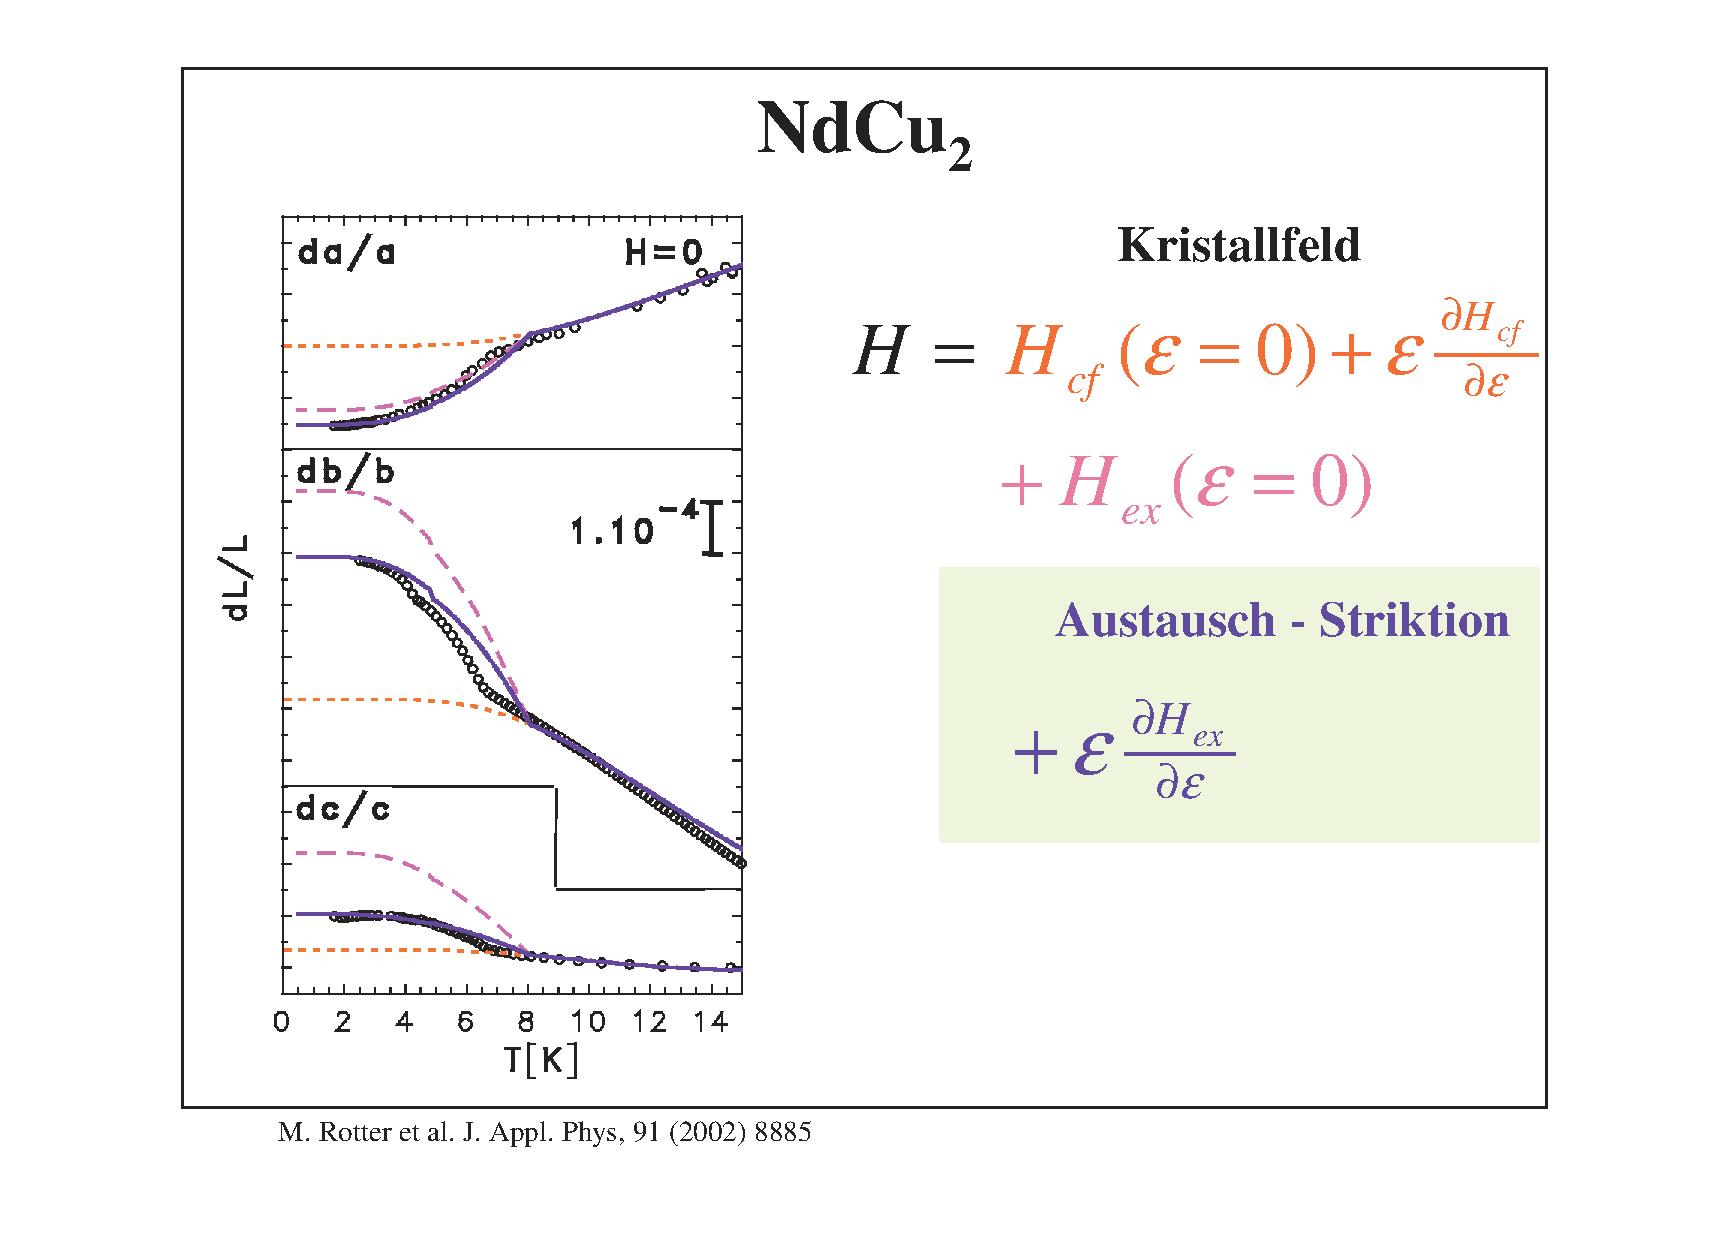
\includegraphics[angle=0, width=0.8\textwidth]{figsrc/magnetostriction_ndcu2.eps}
\end{center}
\caption{Calculated spontaneous magnetostriction of NdCu$_2$.}
\label{magnetostrictiongraphic}
\end{figure}

\begin{description}
\item [\prg mcphas.qvc]    the set of test q-vectors used for calculation of free energy.
                           Components of these q vectors refer to the reciprocal lattice $\vec a^*,\vec b^*,\vec c^*$.
\item [\prg mcphas.phs]    spin-configuration table of different types of spin-configurations. 
                            Note, in case of non-orthogonal axes the convention in these tables 
                            is $mb||\vec b$, $mc||(\vec a \times \vec b)$ and $ma$ perpendicular to $mb$ and $mc$.

                           {\em Note}: 
                           there is no natural criteria for deciding, if one spin-configuration is
			   different from another one. Therefore the list of ''different''
			   spin-configurations is dependent on the meaning of ''different''.
			   
			   The program {\prg McPhase} decides whether a spin-configuration is
			   different from another by a simple criteria, namely by the
			   angle between the spins. Comparing two spin configurations it calculates
			   the angle between corresponding spins and if for one spin the
			   angle is not small, the configuration is treated as a different
			   configuration. Therefore for example a ferromagnet with moments
			   in $a$ has a different spin configuration than a ferromagnet with
			   moments in $b$ direction. 
\item [\prg mcphas.sps]    $T-H$ dependence of spin-configuration. The spin configurations stored in this
                           file may be displayed using the program {\prg spins\index{spins}}, an example is given
			   in figure~\ref{spingraphic}.
                            Note, in case of non-orthogonal axes the convention for applied field $Ha, Hb,Hc$ and
                            also for the moment components $ma, mb, mc$ in these tables 
                            is $mb||\vec b$, $mc||(\vec a \times \vec b)$ and $ma$ perpendicular to $mb$ and $mc$.

\item [\prg mcphas.mf]     $T-H$ dependence of exchange field configuration, stored as $g_J \mu_B H_{xc}(i)$(unit is in meV)
                            for i=1,2,...,number of spins in magnetic unit cell.
                            Note, in case of non-orthogonal axes the convention for applied field $Ha, Hb,Hc$ and
                            also for the mean field components in these tables 
                            is $Hb||\vec b$, $Hc||(\vec a \times \vec b)$ and $Ha$ perpendicular to $Hb$ and $Hc$.
\item [\prg mcphas.fum]    free energy, magnetic energy (the derivative with respect to temperature gives the specific %%@
heat),
                           magnetisation data and (if cfield is used with higher order interactions)
                           expectation values of the Stevens Operators $<O_l^m>$ . As an example for the information
			   contained in this file the calculated magnetisation and magnetostriction of NdCu$_2$ is shown in
			   figures~\ref{magnetization} and ~\ref{magnetizationgraphic}.
                            Note, in case of non-orthogonal axes the convention for applied field $Ha, Hb,Hc$ and
                            also for the magnetisation components $ma,mb,mc$ in these tables 
                            is $Hb||\vec b$, $Hc||(\vec a \times \vec b)$ and $Ha$ perpendicular to $Hb$ and $Hc$.

\item [\prg mcphas1.j1 .j1 .j2 ...] 
               spin-spin correlation functions for sub-lattice 1 neighbour 1 2 ...
	       (linear combination is proportional to magnetostriction)
	       The spin-spin correlation functions for neighbour $k$ are defined by
	       the following sum of dyadic products:

	       \begin{equation}
	        \frac{1}{n}\sum_{s=1}^n <{\mbf J}^s> \times  <{\mbf J}^{s+k}>
	       \end{equation}
	       with $n$ being the number of moments in the magnetic unit cell.
	       Single ion and two-ion magnetostriction can be calculated using the $<O_l^m>$ and the
	       spin-spin correlation functions. As an example the magnetostriction analysis of
	       NdCu$_2$ is shown in figure~\ref{magnetostrictiongraphic}. For details 
             please refer to~\cite{rotter02-8885}.
                            Note, in case of non-orthogonal axes the convention for applied field $Ha, Hb,Hc$ and
                            also for the moment components in these tables 
                            is $Hb||\vec b$, $Hc||(\vec a \times \vec b)$ and $Ha$ perpendicular to $Hb$ and $Hc$.
\item [\prg mcphas.xyt]    phase diagram as x,y,T, H, phase-number j according to spin-configuration table
               given in mcphas.phs, a periodicity key, nettomoments <J>.
 Figure~\ref{phasediagramgraphic}
	       shows the phase diagram of NdCu$_2$ for magnetic fields parallel to the orthorhombic $b$-direction.
                            Note, in case of non-orthogonal axes the convention for applied field $Ha, Hb,Hc$ 
                             in these tables 
                            is $Hb||\vec b$, $Hc||(\vec a \times \vec b)$ and $Ha$ perpendicular to $Hb$ and $Hc$.
\item [\prg mcphas.hkl]    calculated (unpolarised) neutron diffraction data (the calculated magnetic intensities
    correspond to the magnetic structure + Polarisation factor. The
    Lorentz-factor , magnetic form factor and  instrumental corrections are not calculated.)
 As an example figure~\ref{neutintgraphic}
    shows the calculated temperature dependence of magnetic amplitudes for NdCu$_2$.
                           $h,k,l$ refer to the reciprocal lattice $\vec a^*,\vec b^*,\vec c^*$.
                            Note, in case of non-orthogonal axes the convention for applied field $Ha, Hb,Hc$ 
                             in these tables 
                            is $Hb||\vec b$, $Hc||(\vec a \times \vec b)$ and $Ha$ perpendicular to $Hb$ and $Hc$.
    
\item [\prg mcphasa.hkl]    Fourier Transform of the $a$-component of the magnetic Moments.
                           $h,k,l$ refer to the reciprocal lattice $\vec a^*,\vec b^*,\vec c^*$.
                            Note, in case of non-orthogonal axes the convention for applied field $Ha, Hb,Hc$ and
                            the magnetic moment component in these tables 
                            is $Hb||\vec b$, $Hc||(\vec a \times \vec b)$ and $Ha$ perpendicular to $Hb$ and $Hc$.
\item [\prg mcphasb.hkl]    Fourier Transform of the $b$-component of the magnetic Moments.
                           $h,k,l$ refer to the reciprocal lattice $\vec a^*,\vec b^*,\vec c^*$.
                            Note, in case of non-orthogonal axes the convention for applied field $Ha, Hb,Hc$ and
                            the magnetic moment component in these tables 
                            is $Hb||\vec b$, $Hc||(\vec a \times \vec b)$ and $Ha$ perpendicular to $Hb$ and $Hc$.
\item [\prg mcphasc.hkl]    Fourier Transform of the $c$-component of the magnetic Moments.
                           $h,k,l$ refer to the reciprocal lattice $\vec a^*,\vec b^*,\vec c^*$.
                            Note, in case of non-orthogonal axes the convention for applied field $Ha, Hb,Hc$ and
                            the magnetic moment component in these tables 
                            is $Hb||\vec b$, $Hc||(\vec a \times \vec b)$ and $Ha$ perpendicular to $Hb$ and $Hc$.
\end{description} 

\vspace{1cm}
{\em Exercises:}
\begin{itemize}
\item Look at the output files of {\prg McPhase}  in the directory
{\prg examples/ndcu2b\_new/results}.  At which magnetic field
the ferromagnetically aligned state is achieved (at $T=$2~K)?
\item
What is the propagation vector in the different antiferromagnetic phases at $T=$2~K ?
\end{itemize}



\subsubsection{{\prg mcphas.tst\index{mcphas.tst}} - input file of test spin-configurations (optional)}
This file is optional and contains
some test momentum configurations to be used for the calculation
             of the free energy. Mind that
\begin{itemize}
\item  in the file header the number of atoms in the primitive
       crystallographic unit cell and the number of components
       of the spin vector have to be given.
\item  at the end of the
 file there must be no empty lines !
\end{itemize}

The momentum - configurations tables always refer to spins sitting on
the primitive lattice ${\mbf r}_i$. If more than one atom is in
the primitive basis, the momentum gets $3n$ components ($n=$ number
of atoms in the crystallographic basis). See {\prg ./examples/ndcu2b\_new/} for
examples of a two atom basis. Units of these tables are that of total 
angular momentum $<J>$.

\subsubsection{Example {\prg mcphas.tst\index{mcphas.tst}} file  for a simple antiferromagnet}

Here is the file {\prg mcphas.tst\index{mcphas.tst}} for the simple antiferromagnet example
describing some spin configurations
to be used as starting values for the mean field process:

\section{{\prg mcphas} - calculation of thermodynamic properties (Magnetisation, Susceptibility, Specific Heat, Neutron %%@
Diffraction, etc.)}
\label{runmcphas}

In order to perform calculations beyond the capabilities of {\prg cfield\index{cfield}} it is necessary
to use the program {\prg mcphas}. 
\begin{itemize}
\item As a first step it is possible to
calculate the thermodynamic properties such as magnetisation or specific heat
considering only single ion effects. In this case all the exchange parameters
have to be set to zero in {\prg mcphas.j\index{mcphas.j}}. 
\item for more advanced calculations the two - ion interactions have to be
considered and may lead to magnetic order. {\prg mcphas} can perform 
calculations in the ordered state in the following way: for 
a given temperature $T$ and magnetic field $\mbf H$ (vector)
several possible magnetic structures are stabilised
by a mean field algorithm and the free energy is 
calculated. The initial values for this mean-field procedure are
modified by a Monte Carlo process.


The temperature and magnetic field is varied during the calculation
and thereby it is possible to map out the magnetic phase diagram.
\end{itemize}

The program produces a plot of the stabilised magnetic
structures and the magnetisation on screen, the
output files contain additional information 
such as calculated magnetoelastic and  neutron-scattering
data. Several graphic programs easy the visualisation of the
calculated data (section~\ref{graphics}).



\subsection{Input Files}
The program {\prg McPhase} needs the following input files (all in the same directory)
 in order to run:

\begin{enumerate}
\item {\prg mcphas.ini\index{mcphas.ini}}
 - controlling the algorithm
\item {\prg mcphas.j\index{mcphas.j}}
  - lattice and exchange parameters
\item {\prg mcphas.tst\index{mcphas.tst}(optional)}  - test spin configurations
\item {\prg single-ion property files}
\item {\prg directory ./results/}
 - directory where calculated data is stored
\item {\prg directory ./fit} - experimental data for fit (optional)
\end{enumerate}


 All
 of these input files have to be in one directory and the program
has to be started in this directory. The results of the simulation
are then stored in the  subdirectory ./results/, which must exist before starting
the program 
... see directory ./examples/ for some examples.
 In order to prepare these files
for a new calculation it is best to take them from an example, copy the files
to a new directory and make the
modifications  to adapt them to the new problem.

\subsubsection{Example - a simple antiferromagnet}

In the following description of the input files we will always refer
to a simple example: a simple antiferromagnet
on a primitive orthorhombic lattice. The first time user
will thus have a simple example to follow, all corresponding
files are given in the directory {\prg tutorial/03magnetic\_phases\_mcphas/simpleAF}.
 

\subsubsection{{\prg mcphas.ini\index{mcphas.ini}} - controlling the algorithm}
   Initial file containing algorithm control parameters, for instance the range and spacing of
   propagation vectors Q or the number of Monte Carlo trials for initial spin configurations
    - {\em mind}: this
   file is rewritten and reread  when running the program and may be changed by the
   user in order to manipulate the running simulation.

{\prg mcphas.ini\index{mcphas.ini}} consists of several sections:
\begin{description}
\item [MCPHASE RUNTIME CONTROL:] this section contains the parameters
controlling the status of the calculation.
\item [XY PHASEDIAGRAM PARAMETERS:] here the temperature and field range and
step widths of the calculation are specified.
The definition of the x and y
axis in terms of temperature and magnetic field is followed by the
corresponding range and step width. An offset may be given for all
field and temperature values.
Note that for most cases of interest
this offset is zero (T0=0, Ha0=0, Hb0=0, Hc0=0).
 For the simple case of calculating a Temperature-Field phase diagram
 It is just necessary to set xT=1 and give the temperature range by
xmin/xmax/xstep. For field in b direction then just set yHb=1 and 
define the range in ymin/ymax/ystep.
In case of non-orthogonal axes the applied magnetic field
components $Ha, Hb, Hc$ refer to the orthogonal coordinate system
defined with respect to the nonorthogonal lattice $\mbf a,\mbf b,\mbf c$ as
$Hb||\mbf b$, $Hc||(\mbf a \times \mbf b)$ and $Ha$ perpendicular to $Hb$ and $Hc$.

\item [GENERATION OF SPINCONFIGURATIONS:] at the beginning of the program
some initial values of spin configurations are generated from a set of 
propagation vectors. This section defines the range of propagation vectors
and the step width.
Depending on the value of the propagation Q with respect to the primitive reciprocal lattice
1-, 2- or 3-dimensional simulations of magnetic lattices
are possible. It is advisable to 
think carefully about the chosen range and spacing of Q vectors in order
to limit calculation time.
 
For example a good starting point is to begin with a calculation with large
step widths (e.g. 0.1)  covering the Brillouin zone. This should give an idea
of the propagation vectors which are stabilised. An advanced calculation
could then fine tune the propagation and determine its accurate value (using
small step widths in a limited area of the zone).
The verbose option of {\prg mcphas} allows to inspect the propagation vectors
which are actually used in the calculation.
Trick: in order to get a quick overview of the
q-vector range covered by the mcphas\index{mcphas} simulation start mcphas, exit and 
just type {\prg felog ./results/mcphas.qvc} (need {\prg perl,perldl,pdl,pgplot} packages).

In order to limit calculation time, the maximum periodicity
of the magnetic unit cell with respect to the crystallographic unit cell 
(maxqperiod) and the maximum number of spins in the magnetic unit cell 
(maxnofspins) can be limited. Also the maximum number of test spin configurations
in the internal table can be limited (maxnoftestspincf).
A critical feature with respect to calculation time is also the number of
spin configurations which are generated by a random process from a tabulated
SPINCONFIGURATIONS during the calculation. 

In summary the variables in this section are mainly important to adapt the
program to a given computer system with finite speed. They have to be set
to optimise between speed and accuracy of the calculation. In order to
find appropriate values it is best to perform some calculations 
and restrict the parameters step by step if insufficient speed is obtained.
Also the examples included in the program package may serve as starting
points.

\item [PARAMETERS FOR SUB FECALC SELFCONSISTENCY PROCESS:] the most important
procedure in the module {\prg mcphas} is the sub fecalc. In this part of the 
program the self consistent calculation of the magnetic moment configuration
is performed as shown schematically in fig.~\ref{fecalc}. 
In the mean field approximation the Hamiltonian~(\ref{hamilton}) is approximated
by

\begin{equation}
 {\mathcal H}=\sum_n H_{SI}^n + E_{corr}
\end{equation}

with the single ion Hamiltonian (in case of module {\prg so1ion\index{so1ion}})

\begin{equation}
H_{SI}^n=  B_l^m O_{lm}({\mbf J}^n) 
	     - g_{Jn} \mu_B {\mbf J}^n {\mbf H^n_{eff}} 
\end{equation}

and the correction term

\begin{equation}
E_{corr}=\frac{1}{2}\sum_{n} g_{Jn} \mu_B \langle {\mbf J}^n
 \rangle (\mbf H^n_{eff}-\mbf H) 
\end{equation}

and with the mean fields $ \mbf H^n_{eff}$ given by

\begin{equation}\label{meanfield}
\mbf H^n_{eff}=\mbf H + \mbf H^n_{xc}=\mbf H+\sum_{{\mbf G'}n'} \frac{{\mathcal J}
(\mbf r_n-(\mbf G'+\mbf r_{n'}))}{g_{Jn}\mu_B } \langle{\mbf
J}^{n'}\rangle
\end{equation}

These mean fields and the moments $\langle \mbf J^n \rangle$ 
are determined in a self consistent
way. For a given magnetic unit cell and initial configuration 
of magnetic moments
the mean fields are calculated according to equation~(\ref{meanfield}). 
Then, for each
magnetic ion the single ion property module is taken 
and the magnetic moment $\langle \mbf J^n \rangle$ is 
calculated from it's mean field. The mean fields are used again in equation~(\ref{meanfield})
and so on .... until convergence is reached. 
Then, the free energy ($f=-kT\sum_n \ln(z_n) + E_{corr}$ ) 
of the stabilised
configuration is calculated (this is why this sub is called {\prg fecalc}). 
The free energies of a lot of different stabilised configurations have to
be compared in order to find out which configuration has lowest free energy, i.e.
is stable in thermal  equilibrium.

It may happen that this process does
not converge due to bad choice of the initial configuration, therefore a maximum number
of mean field loops has to be given by the user.
The results of a calculation may be significantly influenced by
changing parameters such as the maximum number of iteration loops 
in this section. 
In fact the simulation is always a compromise of calculation time and accuracy: if only
a few initial spin configurations are tried at each (H-T) point, the calculation speed is
fast, however it is possible that the program misses the magnetic structure with the
lowest free energy. The same holds if other critical parameters of the simulation are
restricted too much.
 

\item [OUTPUT OF PHYSICAL PROPERTIES:]
Some options for the output of the calculation can be changed in this section.
\end{description}

\begin{figure}[hb]
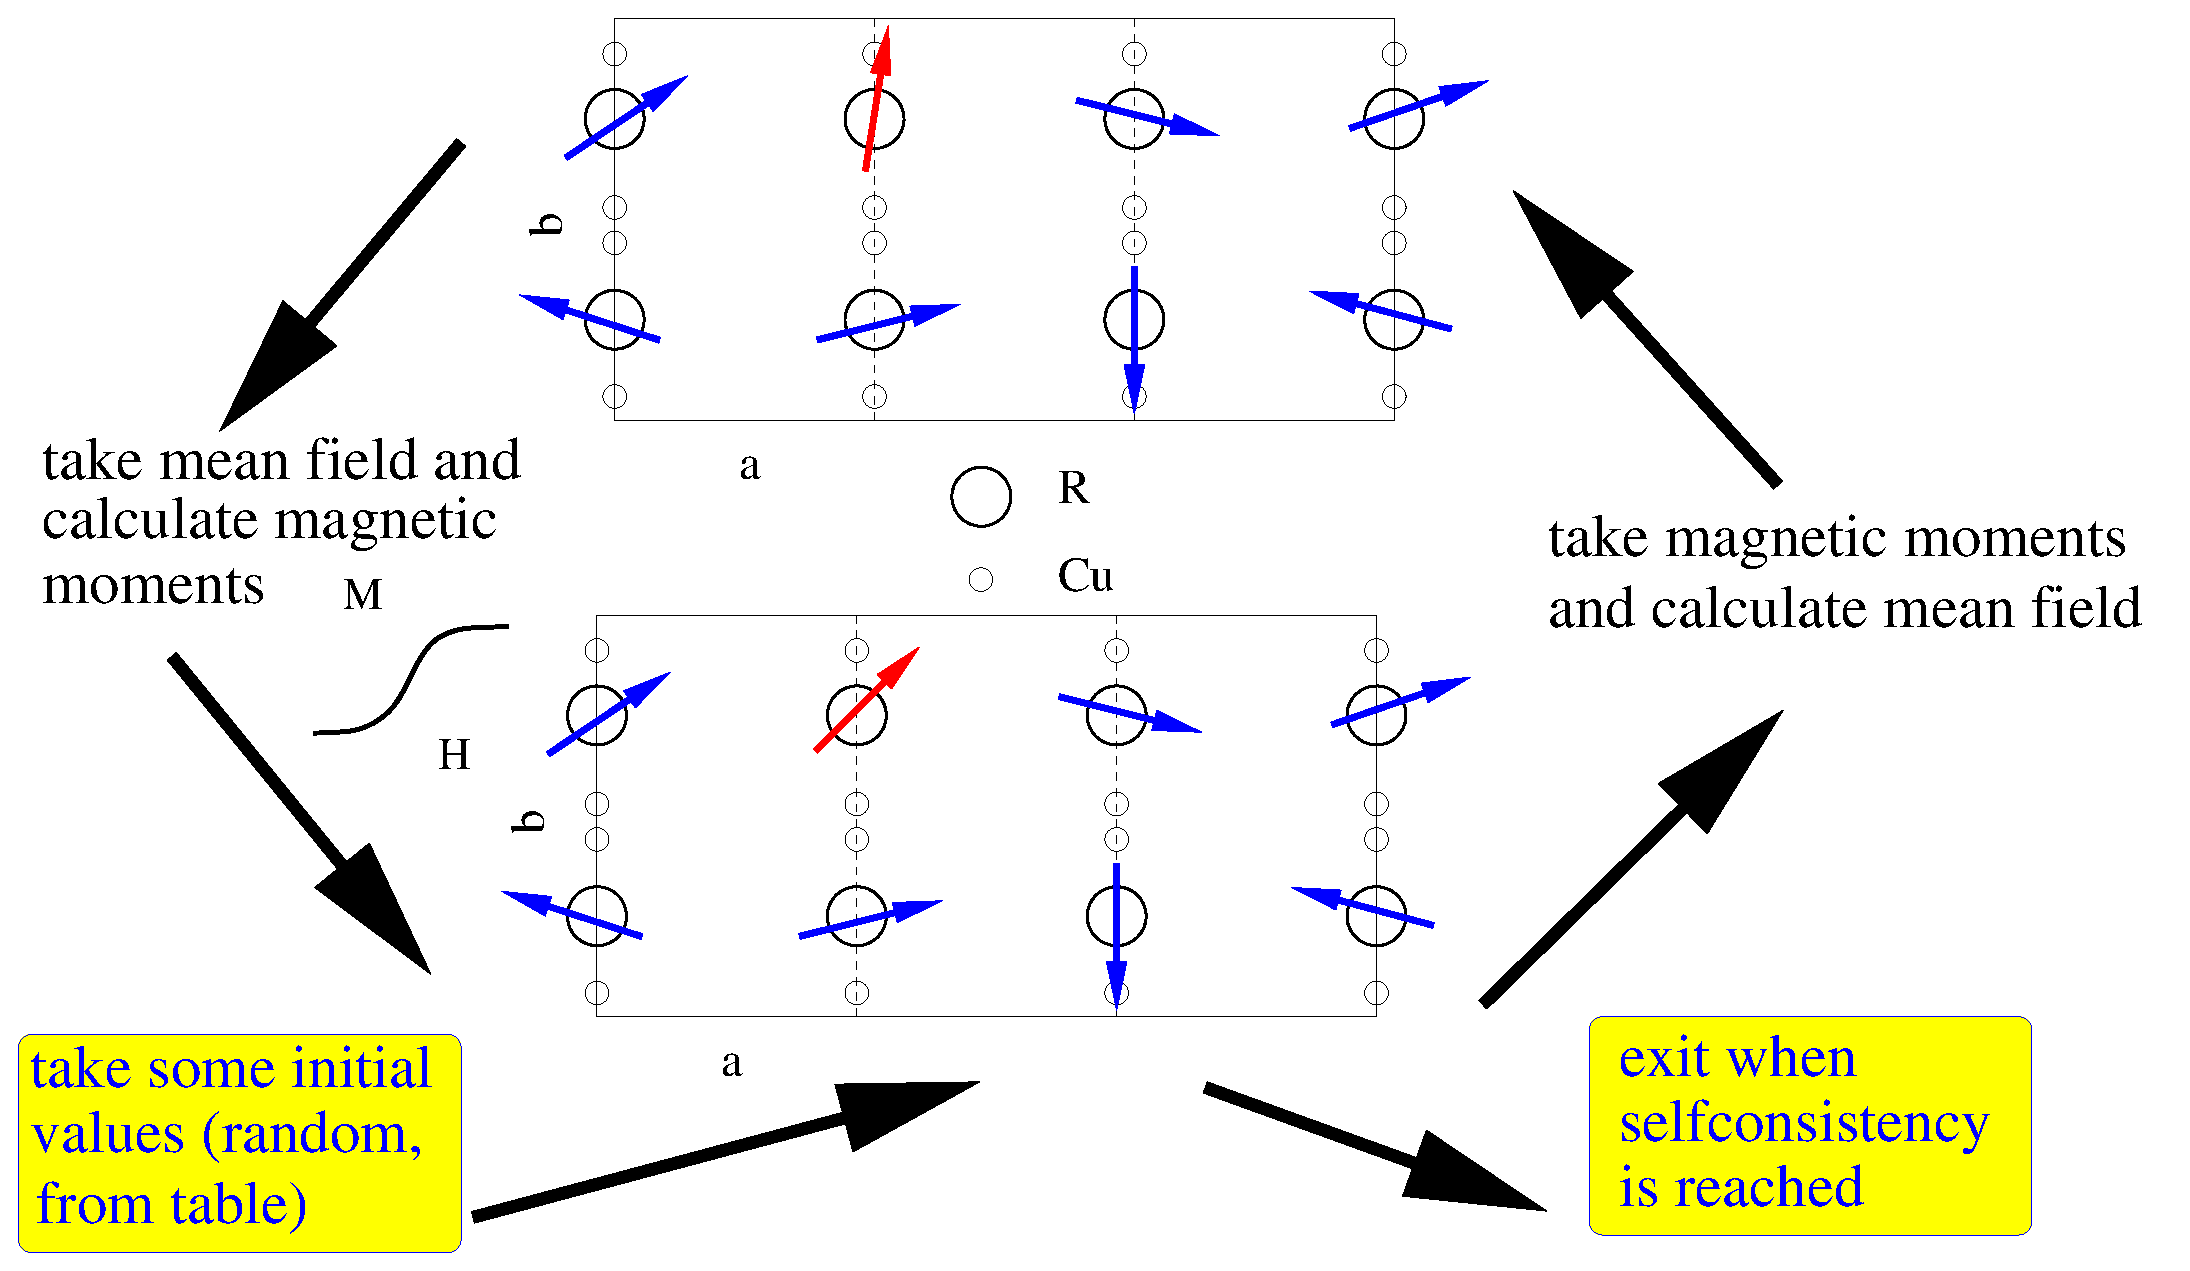
\includegraphics[angle=0,width=0.9\columnwidth]{figsrc/fecalc.eps}
\caption{\label{fecalc}Mean field process of sub {\prg fecalc}.}
\end{figure}

 
\subsubsection{Example {\prg mcphas.ini\index{mcphas.ini}} file for a simple antiferromagnet}

Here is an example of {\prg mcphas.ini\index{mcphas.ini}}, the comments describe the meaning of the different
parameters:

\input{mcphas.ini}



\subsubsection{{\prg mcphas.j\index{mcphas.j}} - lattice and exchange parameters}\label{mcphasj}
This file provides the information about 
the crystallographic
 structure and the magnetic exchange interactions.
For every atom in the crystallographic basis there
has to be given the coordinates, the number of neighbours to be considered, the 
Land\'e factor $g_J$, the single ion property filename and  a set of exchange parameters.
If the exchange parameters (and neighbour positions) are not known for your system, you 
can use the program module {\prg makenn\index{makenn}} (see section \ref{addprog}) to generate 
a list of nearest neighbours and
exchange parameters, currently implemented in {\prg makenn\index{makenn}} are dipolar interactions,
exchange interactions via the Bethe-Slater curve or the RKKY model. Note that in order
to use {\prg makenn\index{makenn}} you have to set up a working {\prg mcphas.j\index{mcphas.j}} file, which may or
may not contain neighbours and interactions.

Use program {\prg addj\index{addj}} to add exchange parameter set stored in different 
such {\prg .j} files (see section~\ref{addprog}).



\begin{description}
\item [Line 1,2:] Comment Lines
\item [Line 3:] lattice constants a,b,c and crystal angles alpha, beta, gamma 
\item [Line 4-6:] primitive lattice vectors
\item [Line 7:] Number of atoms in the primitive crystallographic unit cell ({\prg nofatoms})
\item [Line 8:] a comment line with stars
\item [Line 9:] coordinates  ($d_a$,$d_b$,$d_c$) of 1$^{st}$ magnetic ion in the crystallographic unit cell  with
respect to the lattice vectors $\vec a$,$\vec b$,$\vec c$. The number of neighbours of this 
ion, for which interaction constants are given in the interaction table (nofneighbours). 
If {\prg diagonalexchange}
is set to 0 the 9 components of the exchange tensor are given in column 4-12. 
If {\prg diagonalexchange}
 is 1, only 3 components are given (column 4-6).
If {\prg diagonalexchange}
 is 2, specific components of the exchange tensor can be given in columns 4 onwards. The indices of these components
 must be given in the following line (Line 9a below).
The Land\'e factor of the ion (gJ) and the file name of the corresponding single ion
parameter file (cffilename).
\item [Line 9a:]  If {\prg diagonalexchange=2}, then this line gives the indices of the exchange tensor corresponding to 
 the columns 4 onwards. It must have a variable called {\prg indexexchange} followed by a list of names of components of the interaction
 tensor separated by space. E.g.
 \verb|  #! indexexchange= JaJb JbJc  | 
means column 4 gives the the interaction constant between the
 first angular momentum component of the current ion with the second angular momentum component of its neighbour, whilst 
 column 5 has the interaction constant between the second angular momentum component of this ion with the third component of its
 neighbour. Alternatively, pairs of numbers may be given, as in \verb|  #! indexexchange= 1,2 2,3  |
 Additionally another parameter {\prg symmetricexchange} can be set to 1, where the value in each column is also used 
 for the transposed tensor component. Thus \verb|  #! symmetricexchange=1 indexexchange= JaJb  | is the same as \\
 \verb|  #! indexexchange= JaJb JbJa  | where the 4th and 5th column are the same.
\item [Line 10:]  Comment line
\item [Line 11-(10+nofneighbours):] Interaction table for ion number 1.   
Note: the neighbour coordinates (column 1-3) are given with respect to the lattice vectors
$\vec a$,$\vec b$,$\vec c$. The program then calculates from these values the coordinates
with respect to the primitive lattice $\vec r_1$,~$\vec r_2$,~$\vec r_3$.
($ d_a \vec a + d_b \vec b + d_c \vec c = d_1 \vec r_1 + d_2 \vec r_2 + d_3 \vec r_3$).
Column 4,5,6 \dots contain the components of the interaction tensor $\stackrel{=}{\mathcal J}$. 
Note that in case of non-orthogonal axes the 
components of the moments and the interaction tensor $Ja, Jb, Jc, Jaa, Jbb, Jcc, Jab ...$ 
refer to the orthogonal coordinate system
defined with respect to the nonorthogonal lattice $\vec a,\vec b,\vec c$ as
$Jb||\vec b$, $Jc||(\vec a \times \vec b)$ and $Ja$ perpendicular to $Jb$ and $Jc$.
\item [Line (11+nofneighbours) - end:] for each ion in the unit cell line 8 - (10+nofneighbours)
are repeated.
\end{description}


\vspace{0.5cm}

{\small {\bf Information for experienced users:}
\begin{description}
\item[\prg mcphas.jjj:]
format of exchange parameter file, which only needs a reduced set of exchange
parameters in the input file. Using the program {\prg jjj2j} the file can be transformed
to {\prg mcphas.j\index{mcphas.j}} by adding lines for all the equivalent neighbours. The format definition
of {\prg mcphas.jjj} is the same as {\prg mcphas.j\index{mcphas.j}}, however each line denotes several
equivalent neighbour atoms (instead of only one in {\prg mcphas.j\index{mcphas.j}}) according to the
 following rules:
\begin{itemize}
\item If a nonzero coordinate $d_a$ (or $d_b$,$d_c$) in the interaction table
 corresponds to it's value at the nearest
 lattice point of the primitive lattice,
  additional interactions of the same size
with  neighbours with coordinate $-d_a$ (or $-d_b$,$-d_c$, respectively)
are taken into account. This
holds for each of the three coordinates $d_a$,$d_b$ and $d_c$
 resulting in a maximum
number of 8 equivalent neighbours per line in the interaction table.
\item If the value of $d_a$ (or $d_b$,$d_c$) is zero or differs
from it's value at the nearest lattice point of the primitive lattice, it is 
changed to the value at the nearest lattice point and {\bf no} interaction 
with  neighbours with coordinates $-d_a$ (or $-d_b$,$-d_c$) is
 taken into account. If such
 interaction is needed it may be given in a different line and may
have different magnitude. In this way also crystallographic lattices
with no mirror symmetry may be described.
\end{itemize}
\item[\prg mcphas.coq:]   exchange parameters etc [ in old format]...see examples for details, use {\prg coq2jjj} to 
transform {\prg mcphas.coq} to {\prg mcphas.jjj} format
\end{description}

}


\subsubsection{Example {\prg mcphas.j\index{mcphas.j}} file for a simple antiferromagnet}

Here are example files of a tetragonal antiferromagnet with nearest neighbour interactions, all
files are equivalent:

{\small
\begin{verbatim} 
# simple antiferromagnet 
#<!--mcphase.mcphas.j-->
#***************************************************************
# Lattice Constants (A)
#! a=4.3843 b=4.3843 c=2.4194 alpha=  90 beta=  90 gamma=  90
#! r1a=   1 r2a=   0 r3a=   0
#! r1b=   0 r2b=   1 r3b=   0   primitive lattice vectors [a][b][c]
#! r1c=   0 r2c=   0 r3c=   1
#! nofatoms=1  nofcomponents=3  number of atoms in primitive unit cell/number of components of each spin
# ****************************************************************************
#! da=  0 [a] db=  0 [b] dc=  0 nofneighbours=2 diagonalexchange=0 gJ=0.857143 cffilename=Ce3p.sipf
# da[a] db[b] dc[c] Jaa[meV] Jbb[meV] Jcc[meV] Jab[meV] Jba[meV] Jac[meV] Jca[meV] Jbc[meV] Jcb[meV]
+0	+0	+1	-0.1	-0.1	-0.1   0  0  0  0  0  0
+0	+0	-1	-0.1	-0.1	-0.1   0  0  0  0  0  0
#\end{verbatim}
}

Using diagonalexchange this may be shortened to

{\small
\begin{verbatim} 
# simple antiferromagnet 
#<!--mcphase.mcphas.j-->
#***************************************************************
# Lattice Constants (A)
#! a=4.3843 b=4.3843 c=2.4194 alpha=  90 beta=  90 gamma=  90
#! r1a=   1 r2a=   0 r3a=   0
#! r1b=   0 r2b=   1 r3b=   0   primitive lattice vectors [a][b][c]
#! r1c=   0 r2c=   0 r3c=   1
#! nofatoms=1  nofcomponents=3  number of atoms in primitive unit cell/number of components of each spin
# ****************************************************************************
#! da=  0 [a] db=  0 [b] dc=  0 nofneighbours=2 diagonalexchange=1 gJ=0.857143 cffilename=Ce3p.sipf
# da[a] db[b] dc[c] Jaa[meV] Jbb[meV] Jcc[meV] Jab[meV] Jba[meV] Jac[meV] Jca[meV] Jbc[meV] Jcb[meV]
+0	+0	+1	-0.1	-0.1	-0.1   
+0	+0	-1	-0.1	-0.1	-0.1   
#\end{verbatim}
}

with indexexchange option the sequence of two ion interaction parameters can be changed and
zero parameters may be omitted:

{\small
\begin{verbatim} 
# simple antiferromagnet 
#<!--mcphase.mcphas.j-->
#***************************************************************
# Lattice Constants (A)
#! a=4.3843 b=4.3843 c=2.4194 alpha=  90 beta=  90 gamma=  90
#! r1a=   1 r2a=   0 r3a=   0
#! r1b=   0 r2b=   1 r3b=   0   primitive lattice vectors [a][b][c]
#! r1c=   0 r2c=   0 r3c=   1
#! nofatoms=1  nofcomponents=3  number of atoms in primitive unit cell/number of components of each spin
# ****************************************************************************
#! da=  0 [a] db=  0 [b] dc=  0 nofneighbours=2 diagonalexchange=2 gJ=0.857143 cffilename=Ce3p.sipf
# da[a] db[b] dc[c] Jaa[meV] Jbb[meV] Jcc[meV] Jab[meV] Jba[meV] Jac[meV] Jca[meV] Jbc[meV] Jcb[meV]
#! indexexchange = JaJa JaJc JcJa JbJb JcJc
+0	+0	+1	-0.1 0 0 -0.1	-0.1  
+0	+0	-1	-0.1 0 0 -0.1	-0.1  
#\end{verbatim}
}

{\small
\begin{verbatim} 
# simple antiferromagnet 
#<!--mcphase.mcphas.j-->
#***************************************************************
# Lattice Constants (A)
#! a=4.3843 b=4.3843 c=2.4194 alpha=  90 beta=  90 gamma=  90
#! r1a=   1 r2a=   0 r3a=   0
#! r1b=   0 r2b=   1 r3b=   0   primitive lattice vectors [a][b][c]
#! r1c=   0 r2c=   0 r3c=   1
#! nofatoms=1  nofcomponents=3  number of atoms in primitive unit cell/number of components of each spin
# ****************************************************************************
#! da=  0 [a] db=  0 [b] dc=  0 nofneighbours=2 diagonalexchange=2 gJ=0.857143 cffilename=Ce3p.sipf
# da[a] db[b] dc[c] Jaa[meV] Jbb[meV] Jcc[meV] Jab[meV] Jba[meV] Jac[meV] Jca[meV] Jbc[meV] Jcb[meV]
#! indexexchange = 1,1 1,3, 3,1 2,2 3,3
+0	+0	+1	-0.1 0 0 -0.1	-0.1  
+0	+0	-1	-0.1 0 0 -0.1	-0.1  
#\end{verbatim}
}


using symmetricexchange together with indexexchange will assume that the interaction tensor is symmetic and 
only half of it may be given:

{\small
\begin{verbatim} 
# simple antiferromagnet 
#<!--mcphase.mcphas.j-->
#***************************************************************
# Lattice Constants (A)
#! a=4.3843 b=4.3843 c=2.4194 alpha=  90 beta=  90 gamma=  90
#! r1a=   1 r2a=   0 r3a=   0
#! r1b=   0 r2b=   1 r3b=   0   primitive lattice vectors [a][b][c]
#! r1c=   0 r2c=   0 r3c=   1
#! nofatoms=1  nofcomponents=3  number of atoms in primitive unit cell/number of components of each spin
# ****************************************************************************
#! da=  0 [a] db=  0 [b] dc=  0 nofneighbours=2 diagonalexchange=2 gJ=0.857143 cffilename=Ce3p.sipf
# da[a] db[b] dc[c] Jaa[meV] Jbb[meV] Jcc[meV] Jab[meV] Jba[meV] Jac[meV] Jca[meV] Jbc[meV] Jcb[meV]
#! symmetricexchange=1 indexexchange = JaJa JaJc JbJb JcJc
+0	+0	+1	-0.1 0  -0.1	-0.1  
+0	+0	-1	-0.1 0  -0.1	-0.1  
#\end{verbatim}
}


\subsubsection{Single Ion Property Input Files}\label{sifile}

In order to speed up calculations or treat special problems a large 
variety of single ion modules is available. This includes the
option to load a user written single ion module. Details are 
given in chapter~\ref{simod}.

The first time user of {\prg McPhase} should use the module {\prg so1ion}\index{so1ion} and 
create an appropriate single ion property input file as described in
section \ref{cf1ion}. A good starting point are several examples
given in directory {\prg examples}.


\subsubsection{Example single ion property file  for a simple antiferromagnet}

Here is an example file {\prg mcphas.cf1} describing the anisotropy of a 
simple antiferromagnet with Ce atoms having basal plane anisotropy. Note the
axis convention xyz$||$abc, in case of non-orthogonal axes the convention 
is $y||\vec b$, $z||(\vec a \times \vec b)$ and $x$ perpendicular to $y$ and $z$.


\input{mcphas.cf1}

\subsubsection{{\prg mcphas.tst\index{mcphas.tst}} - input file of test spin-configurations (optional)}
This file is optional and contains
some test momentum configurations to be used for the calculation
             of the free energy. Mind that
\begin{itemize}
\item  in the file header the number of atoms in the primitive
       crystallographic unit cell and the number of components
       of the spin vector have to be given.
\item  at the end of the
 file there must be no empty lines !
\end{itemize}

The momentum - configurations tables always refer to spins sitting on
the primitive lattice ${\mbf r}_i$. If more than one atom is in
the primitive basis, the momentum gets $3n$ components ($n=$ number
of atoms in the crystallographic basis). See {\prg ./examples/ndcu2b\_new/} for
examples of a two atom basis. Units of these tables are that of total 
angular momentum $<J>$.

\subsubsection{Example {\prg mcphas.tst\index{mcphas.tst}} file  for a simple antiferromagnet}

Here is the file {\prg mcphas.tst\index{mcphas.tst}} for the simple antiferromagnet example
describing some spin configurations
to be used as starting values for the mean field process:

\input{mcphas.tst}
Note, in case of non-orthogonal axes the convention 
is $mb||\vec b$, $mc||(\vec a \times \vec b)$ and $ma$ perpendicular to $mb$ and $mc$.

\subsubsection{subdirectory {\prg ./results} - directory where calculated data is stored}

In order to be able to save the results of a calculation the directory {\prg ./results} has to
exist. Mind that all files in this directory will be overwritten without warning. 

\subsubsection{subdirectory {\prg ./fit} - experimental data for fit (optional) } 

In order that {\prg McPhase} can calculate the standard deviation between
 experimental data and the results of the simulation, some experimental data
 can be given in the subdirectory {\prg ./fit}. The filenames and the data-format
 are the same as the output files of {\prg McPhas}, e.g. {\prg mcphas.fum}, {\prg mcphas.hkl}
 etc. {\prg McPhase} looks into the directory {\prg ./fit} and if it finds any
 of these files, the standard deviation is increased correspondingly. 

What measurement data can be used to calculate a standard deviation ?

\begin{description}
\item[{\prg mcphas.fum}] if given in column 11, 12, 13 in {\prg ./fit/mcphas.fum} the
            magnetisation in the $a$, $b$ and $c$ direction is used for calculation
	    of the standard deviation sta. The standard deviation is calculated
	    as ${\rm sta}=\sum_{\rm data points i} ({\mbf m}_i^{calc}-{\mbf m}_i^{meas})^2$.
	    All three components of the magnetic moment have to be given and are used.

\end{description}

Note that the measured data has to be given in those (H-T) points which are 
calculated by mcphas\index{mcphas} in order to be used by the program to increase {\prg sta}.
It is usually most effective to fit only few data points, because a large set
of data points will not improve the quality of the fit and only require a large
amount of calculation time.



\subsection{Starting a simulation}
\label{start}

To start the simulation goto the directory containing the
input files {\prg mcphas.ini, mcphas.j, etc. } and type

\begin{description}
\item[\prg mcphas] to run the program generating stepwise $H-T$ values 
              in a loop given by {\prg mcphas.ini\index{mcphas.ini}} (you can also press the
              symbol in the {\prg McPhase - Explorer} window).
\item[\prg mcphas\index{mcphas} [file]]  to run the program with an input file --   
             {\prg file} contains T ha hb hc values to be calculated 
             if [file] is not given, xmin xmax xstep (xT xHa xHb xHc)
             ymin ymax ystep (yT yHa yHb yHc) is read from file {\prg mcphas.ini\index{mcphas.ini}}
	     and phase diagram is calculated
\item[\prg mcphas\index{mcphas} -h]  to  print help and version of {\prg McPhas}.
\item[\prg mcphas\index{mcphas} -stamax 14]  end mcphas\index{mcphas} if standard deviation exceeds 14.
\item[\prg mcphas\index{mcphas} -a] avoid overwriting output files in results, append new results to existing files
\item[\prg mcphas\index{mcphas} -v]  to  enable verbose mode with lots of messages of {\prg McPhas}. Specifically
the verbose mode enables the following features:
  \begin{itemize}
			          \item more information is printed out, 
			          \item the q-vectors file {\prg ./results/mcphas.qvc} will contain 
				    the explicit spin configurations
			          \item the display\index{display} on screen (ghostview window using 
				     {\prg ./results/.sps.eps}) will be updated not only 
				    when a H-T point has been finished but always 
				    when a structure with smaller free energy 
				    has been stabilised
  \end{itemize}
\item[\prg mcphasit\index{mcphas}] to start mcphase in commandline mode without opening any window
\end{description}

\vspace{1cm}
{\em Exercises:}
\begin{itemize}
\item Look at the input files for {\prg McPhase} given in the directory
{\prg examples/ndcu2b\_new}.  How many atoms are contained in the crystallographic basis ?
\item
Start the simulation by typing the command {\prg mcphas}.
\end{itemize}



\subsection{Options for a running simulation}
... when the program is running, the options in the main window
can be changed. Pressing ''displayall'' displays the current spin-configuration
at each iteration step. Pressing ''log fe vs Q'' appends free energy vs Q
data to {\prg mcphas.log} for every ($T-H$) point.


The file {\prg ./results/.spins.eps} is used to show the information about the currently calculated
spin structure on the screen using the postscript file viewer ghostview.

The file {\prg ./results/.mcphas.fum} contains the information of the magnetisation curve
which is currently calculated. This information is automatically displayed on the screen.


The program {\prg display} (see section \ref{display}) can be used 
for the online display\index{display} of any other
curve(s).


\subsection{Output Files - {\prg mcphas.qvc,phs,sps,mf,fum,j1...,xyt,hkl} }\label{outputfiles}
 (in directory ./results/ after a simulation run) 

\begin{figure}[htb]%h=here, t=top, b=bottom, p=separate figure page
\begin{center}\leavevmode
\includegraphics[angle=0, width=0.3\textwidth]{figsrc/magnetization_ndcu2.ps}
\end{center}
\caption{Calculated magnetisation of NdCu$_2$ for field parallel to the orthorhombic $b$-direction.}
\label{magnetization}
\end{figure}

\begin{figure}[htb]%h=here, t=top, b=bottom, p=separate figure page
\begin{center}\leavevmode
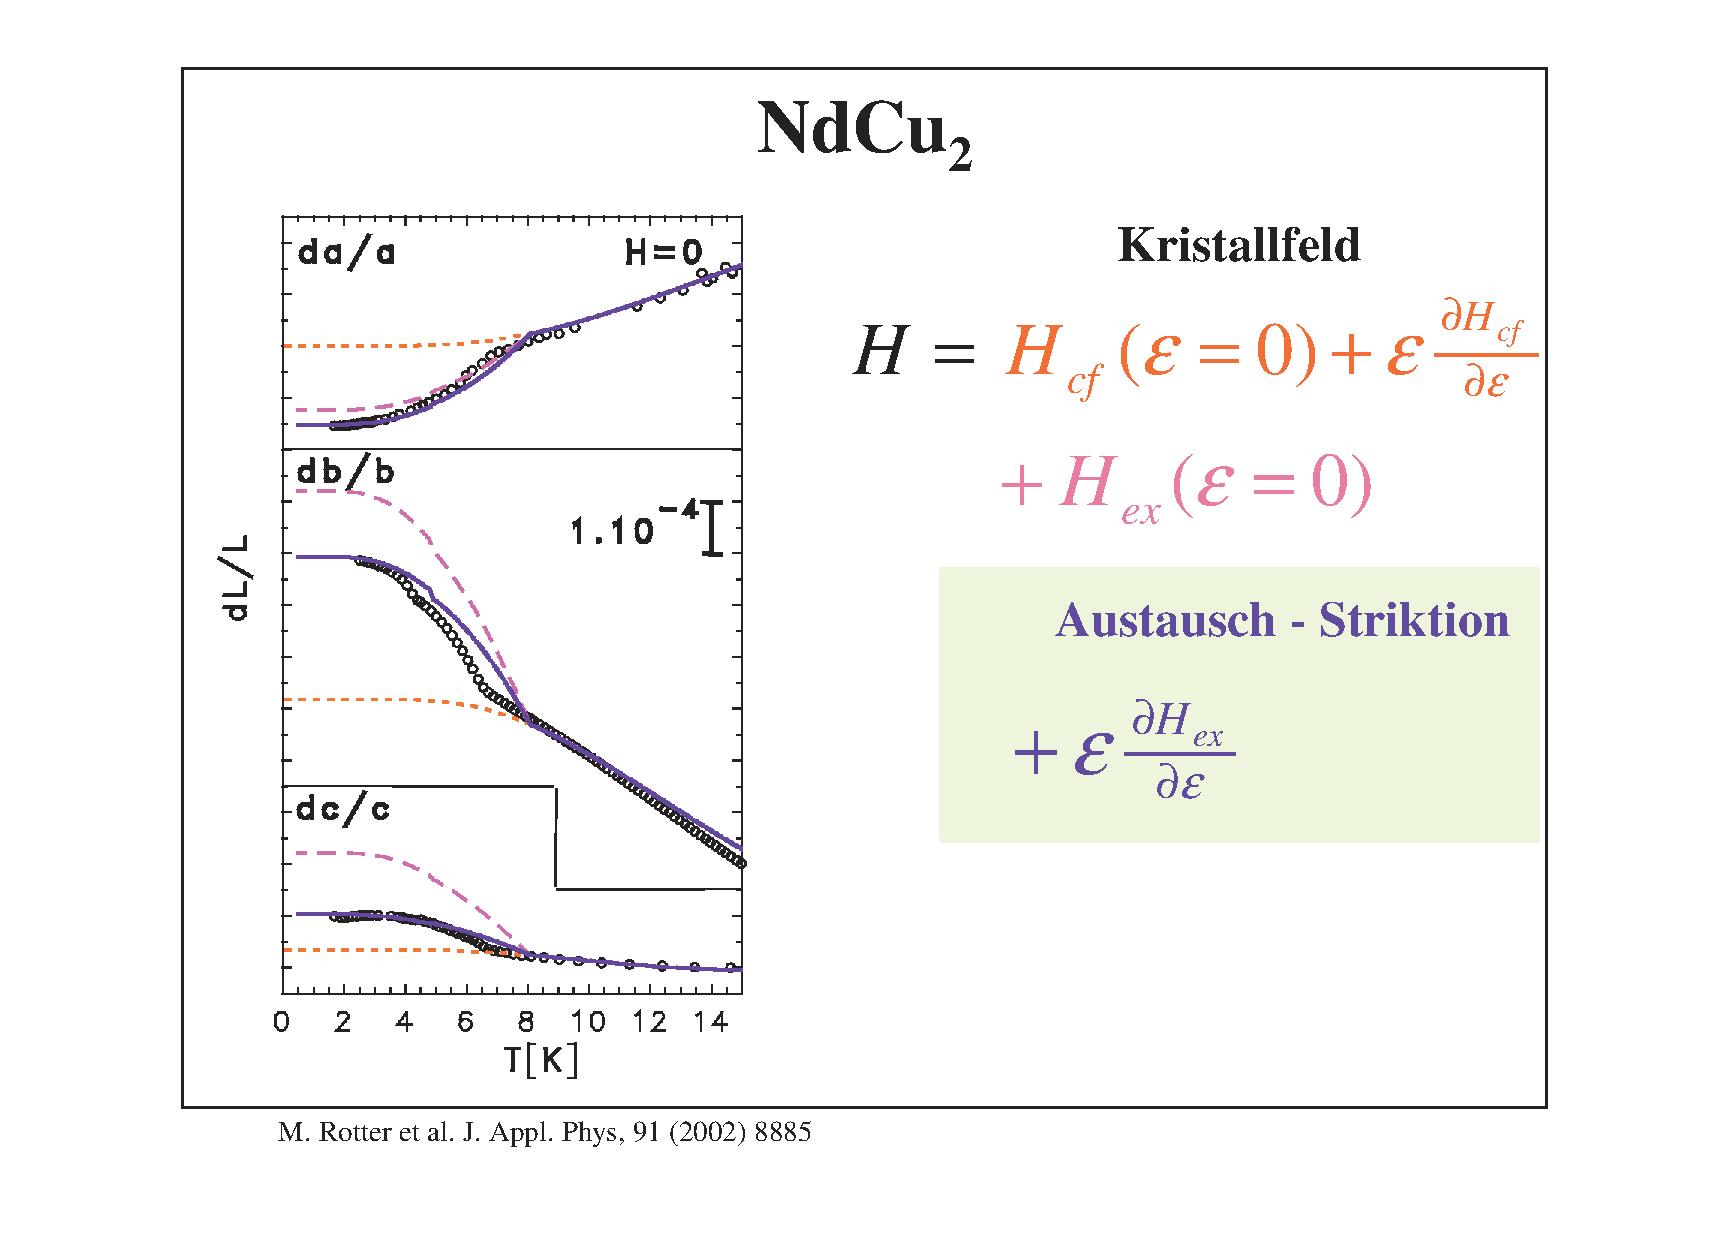
\includegraphics[angle=0, width=0.8\textwidth]{figsrc/magnetostriction_ndcu2.eps}
\end{center}
\caption{Calculated spontaneous magnetostriction of NdCu$_2$.}
\label{magnetostrictiongraphic}
\end{figure}

\begin{description}
\item [\prg mcphas.qvc]    the set of test q-vectors used for calculation of free energy.
                           Components of these q vectors refer to the reciprocal lattice $\vec a^*,\vec b^*,\vec c^*$.
\item [\prg mcphas.phs]    spin-configuration table of different types of spin-configurations. 
                            Note, in case of non-orthogonal axes the convention in these tables 
                            is $mb||\vec b$, $mc||(\vec a \times \vec b)$ and $ma$ perpendicular to $mb$ and $mc$.

                           {\em Note}: 
                           there is no natural criteria for deciding, if one spin-configuration is
			   different from another one. Therefore the list of ''different''
			   spin-configurations is dependent on the meaning of ''different''.
			   
			   The program {\prg McPhase} decides whether a spin-configuration is
			   different from another by a simple criteria, namely by the
			   angle between the spins. Comparing two spin configurations it calculates
			   the angle between corresponding spins and if for one spin the
			   angle is not small, the configuration is treated as a different
			   configuration. Therefore for example a ferromagnet with moments
			   in $a$ has a different spin configuration than a ferromagnet with
			   moments in $b$ direction. 
\item [\prg mcphas.sps]    $T-H$ dependence of spin-configuration. The spin configurations stored in this
                           file may be displayed using the program {\prg spins\index{spins}}, an example is given
			   in figure~\ref{spingraphic}.
                            Note, in case of non-orthogonal axes the convention for applied field $Ha, Hb,Hc$ and
                            also for the moment components $ma, mb, mc$ in these tables 
                            is $mb||\vec b$, $mc||(\vec a \times \vec b)$ and $ma$ perpendicular to $mb$ and $mc$.

\item [\prg mcphas.mf]     $T-H$ dependence of exchange field configuration, stored as $g_J \mu_B H_{xc}(i)$(unit is in meV)
                            for i=1,2,...,number of spins in magnetic unit cell.
                            Note, in case of non-orthogonal axes the convention for applied field $Ha, Hb,Hc$ and
                            also for the mean field components in these tables 
                            is $Hb||\vec b$, $Hc||(\vec a \times \vec b)$ and $Ha$ perpendicular to $Hb$ and $Hc$.
\item [\prg mcphas.fum]    free energy, magnetic energy (the derivative with respect to temperature gives the specific %%@
heat),
                           magnetisation data and (if cfield is used with higher order interactions)
                           expectation values of the Stevens Operators $<O_l^m>$ . As an example for the information
			   contained in this file the calculated magnetisation and magnetostriction of NdCu$_2$ is shown in
			   figures~\ref{magnetization} and ~\ref{magnetizationgraphic}.
                            Note, in case of non-orthogonal axes the convention for applied field $Ha, Hb,Hc$ and
                            also for the magnetisation components $ma,mb,mc$ in these tables 
                            is $Hb||\vec b$, $Hc||(\vec a \times \vec b)$ and $Ha$ perpendicular to $Hb$ and $Hc$.

\item [\prg mcphas1.j1 .j1 .j2 ...] 
               spin-spin correlation functions for sub-lattice 1 neighbour 1 2 ...
	       (linear combination is proportional to magnetostriction)
	       The spin-spin correlation functions for neighbour $k$ are defined by
	       the following sum of dyadic products:

	       \begin{equation}
	        \frac{1}{n}\sum_{s=1}^n <{\mbf J}^s> \times  <{\mbf J}^{s+k}>
	       \end{equation}
	       with $n$ being the number of moments in the magnetic unit cell.
	       Single ion and two-ion magnetostriction can be calculated using the $<O_l^m>$ and the
	       spin-spin correlation functions. As an example the magnetostriction analysis of
	       NdCu$_2$ is shown in figure~\ref{magnetostrictiongraphic}. For details 
             please refer to~\cite{rotter02-8885}.
                            Note, in case of non-orthogonal axes the convention for applied field $Ha, Hb,Hc$ and
                            also for the moment components in these tables 
                            is $Hb||\vec b$, $Hc||(\vec a \times \vec b)$ and $Ha$ perpendicular to $Hb$ and $Hc$.
\item [\prg mcphas.xyt]    phase diagram as x,y,T, H, phase-number j according to spin-configuration table
               given in mcphas.phs, a periodicity key, nettomoments <J>.
 Figure~\ref{phasediagramgraphic}
	       shows the phase diagram of NdCu$_2$ for magnetic fields parallel to the orthorhombic $b$-direction.
                            Note, in case of non-orthogonal axes the convention for applied field $Ha, Hb,Hc$ 
                             in these tables 
                            is $Hb||\vec b$, $Hc||(\vec a \times \vec b)$ and $Ha$ perpendicular to $Hb$ and $Hc$.
\item [\prg mcphas.hkl]    calculated (unpolarised) neutron diffraction data (the calculated magnetic intensities
    correspond to the magnetic structure + Polarisation factor. The
    Lorentz-factor , magnetic form factor and  instrumental corrections are not calculated.)
 As an example figure~\ref{neutintgraphic}
    shows the calculated temperature dependence of magnetic amplitudes for NdCu$_2$.
                           $h,k,l$ refer to the reciprocal lattice $\vec a^*,\vec b^*,\vec c^*$.
                            Note, in case of non-orthogonal axes the convention for applied field $Ha, Hb,Hc$ 
                             in these tables 
                            is $Hb||\vec b$, $Hc||(\vec a \times \vec b)$ and $Ha$ perpendicular to $Hb$ and $Hc$.
    
\item [\prg mcphasa.hkl]    Fourier Transform of the $a$-component of the magnetic Moments.
                           $h,k,l$ refer to the reciprocal lattice $\vec a^*,\vec b^*,\vec c^*$.
                            Note, in case of non-orthogonal axes the convention for applied field $Ha, Hb,Hc$ and
                            the magnetic moment component in these tables 
                            is $Hb||\vec b$, $Hc||(\vec a \times \vec b)$ and $Ha$ perpendicular to $Hb$ and $Hc$.
\item [\prg mcphasb.hkl]    Fourier Transform of the $b$-component of the magnetic Moments.
                           $h,k,l$ refer to the reciprocal lattice $\vec a^*,\vec b^*,\vec c^*$.
                            Note, in case of non-orthogonal axes the convention for applied field $Ha, Hb,Hc$ and
                            the magnetic moment component in these tables 
                            is $Hb||\vec b$, $Hc||(\vec a \times \vec b)$ and $Ha$ perpendicular to $Hb$ and $Hc$.
\item [\prg mcphasc.hkl]    Fourier Transform of the $c$-component of the magnetic Moments.
                           $h,k,l$ refer to the reciprocal lattice $\vec a^*,\vec b^*,\vec c^*$.
                            Note, in case of non-orthogonal axes the convention for applied field $Ha, Hb,Hc$ and
                            the magnetic moment component in these tables 
                            is $Hb||\vec b$, $Hc||(\vec a \times \vec b)$ and $Ha$ perpendicular to $Hb$ and $Hc$.
\end{description} 

\vspace{1cm}
{\em Exercises:}
\begin{itemize}
\item Look at the output files of {\prg McPhase}  in the directory
{\prg examples/ndcu2b\_new/results}.  At which magnetic field
the ferromagnetically aligned state is achieved (at $T=$2~K)?
\item
What is the propagation vector in the different antiferromagnetic phases at $T=$2~K ?
\end{itemize}


Note, in case of non-orthogonal axes the convention 
is $mb||\vec b$, $mc||(\vec a \times \vec b)$ and $ma$ perpendicular to $mb$ and $mc$.

\subsubsection{subdirectory {\prg ./results} - directory where calculated data is stored}

In order to be able to save the results of a calculation the directory {\prg ./results} has to
exist. Mind that all files in this directory will be overwritten without warning. 

\subsubsection{subdirectory {\prg ./fit} - experimental data for fit (optional) } 

In order that {\prg McPhase} can calculate the standard deviation between
 experimental data and the results of the simulation, some experimental data
 can be given in the subdirectory {\prg ./fit}. The filenames and the data-format
 are the same as the output files of {\prg McPhas}, e.g. {\prg mcphas.fum}, {\prg mcphas.hkl}
 etc. {\prg McPhase} looks into the directory {\prg ./fit} and if it finds any
 of these files, the standard deviation is increased correspondingly. 

What measurement data can be used to calculate a standard deviation ?

\begin{description}
\item[{\prg mcphas.fum}] if given in column 11, 12, 13 in {\prg ./fit/mcphas.fum} the
            magnetisation in the $a$, $b$ and $c$ direction is used for calculation
	    of the standard deviation sta. The standard deviation is calculated
	    as ${\rm sta}=\sum_{\rm data points i} ({\mbf m}_i^{calc}-{\mbf m}_i^{meas})^2$.
	    All three components of the magnetic moment have to be given and are used.

\end{description}

Note that the measured data has to be given in those (H-T) points which are 
calculated by mcphas\index{mcphas} in order to be used by the program to increase {\prg sta}.
It is usually most effective to fit only few data points, because a large set
of data points will not improve the quality of the fit and only require a large
amount of calculation time.



\subsection{Starting a simulation}
\label{start}

To start the simulation goto the directory containing the
input files {\prg mcphas.ini, mcphas.j, etc. } and type

\begin{description}
\item[\prg mcphas] to run the program generating stepwise $H-T$ values 
              in a loop given by {\prg mcphas.ini\index{mcphas.ini}} (you can also press the
              symbol in the {\prg McPhase - Explorer} window).
\item[\prg mcphas\index{mcphas} [file]]  to run the program with an input file --   
             {\prg file} contains T ha hb hc values to be calculated 
             if [file] is not given, xmin xmax xstep (xT xHa xHb xHc)
             ymin ymax ystep (yT yHa yHb yHc) is read from file {\prg mcphas.ini\index{mcphas.ini}}
	     and phase diagram is calculated
\item[\prg mcphas\index{mcphas} -h]  to  print help and version of {\prg McPhas}.
\item[\prg mcphas\index{mcphas} -stamax 14]  end mcphas\index{mcphas} if standard deviation exceeds 14.
\item[\prg mcphas\index{mcphas} -a] avoid overwriting output files in results, append new results to existing files
\item[\prg mcphas\index{mcphas} -v]  to  enable verbose mode with lots of messages of {\prg McPhas}. Specifically
the verbose mode enables the following features:
  \begin{itemize}
			          \item more information is printed out, 
			          \item the q-vectors file {\prg ./results/mcphas.qvc} will contain 
				    the explicit spin configurations
			          \item the display\index{display} on screen (ghostview window using 
				     {\prg ./results/.sps.eps}) will be updated not only 
				    when a H-T point has been finished but always 
				    when a structure with smaller free energy 
				    has been stabilised
  \end{itemize}
\item[\prg mcphasit\index{mcphas}] to start mcphase in commandline mode without opening any window
\end{description}

\vspace{1cm}
{\em Exercises:}
\begin{itemize}
\item Look at the input files for {\prg McPhase} given in the directory
{\prg examples/ndcu2b\_new}.  How many atoms are contained in the crystallographic basis ?
\item
Start the simulation by typing the command {\prg mcphas}.
\end{itemize}



\subsection{Options for a running simulation}
... when the program is running, the options in the main window
can be changed. Pressing ''displayall'' displays the current spin-configuration
at each iteration step. Pressing ''log fe vs Q'' appends free energy vs Q
data to {\prg mcphas.log} for every ($T-H$) point.


The file {\prg ./results/.spins.eps} is used to show the information about the currently calculated
spin structure on the screen using the postscript file viewer ghostview.

The file {\prg ./results/.mcphas.fum} contains the information of the magnetisation curve
which is currently calculated. This information is automatically displayed on the screen.


The program {\prg display} (see section \ref{display}) can be used 
for the online display\index{display} of any other
curve(s).


\subsection{Output Files - {\prg mcphas.qvc,phs,sps,mf,fum,j1...,xyt,hkl} }\label{outputfiles}
 (in directory ./results/ after a simulation run) 

\begin{figure}[htb]%h=here, t=top, b=bottom, p=separate figure page
\begin{center}\leavevmode
\includegraphics[angle=0, width=0.3\textwidth]{figsrc/magnetization_ndcu2.ps}
\end{center}
\caption{Calculated magnetisation of NdCu$_2$ for field parallel to the orthorhombic $b$-direction.}
\label{magnetization}
\end{figure}

\begin{figure}[htb]%h=here, t=top, b=bottom, p=separate figure page
\begin{center}\leavevmode
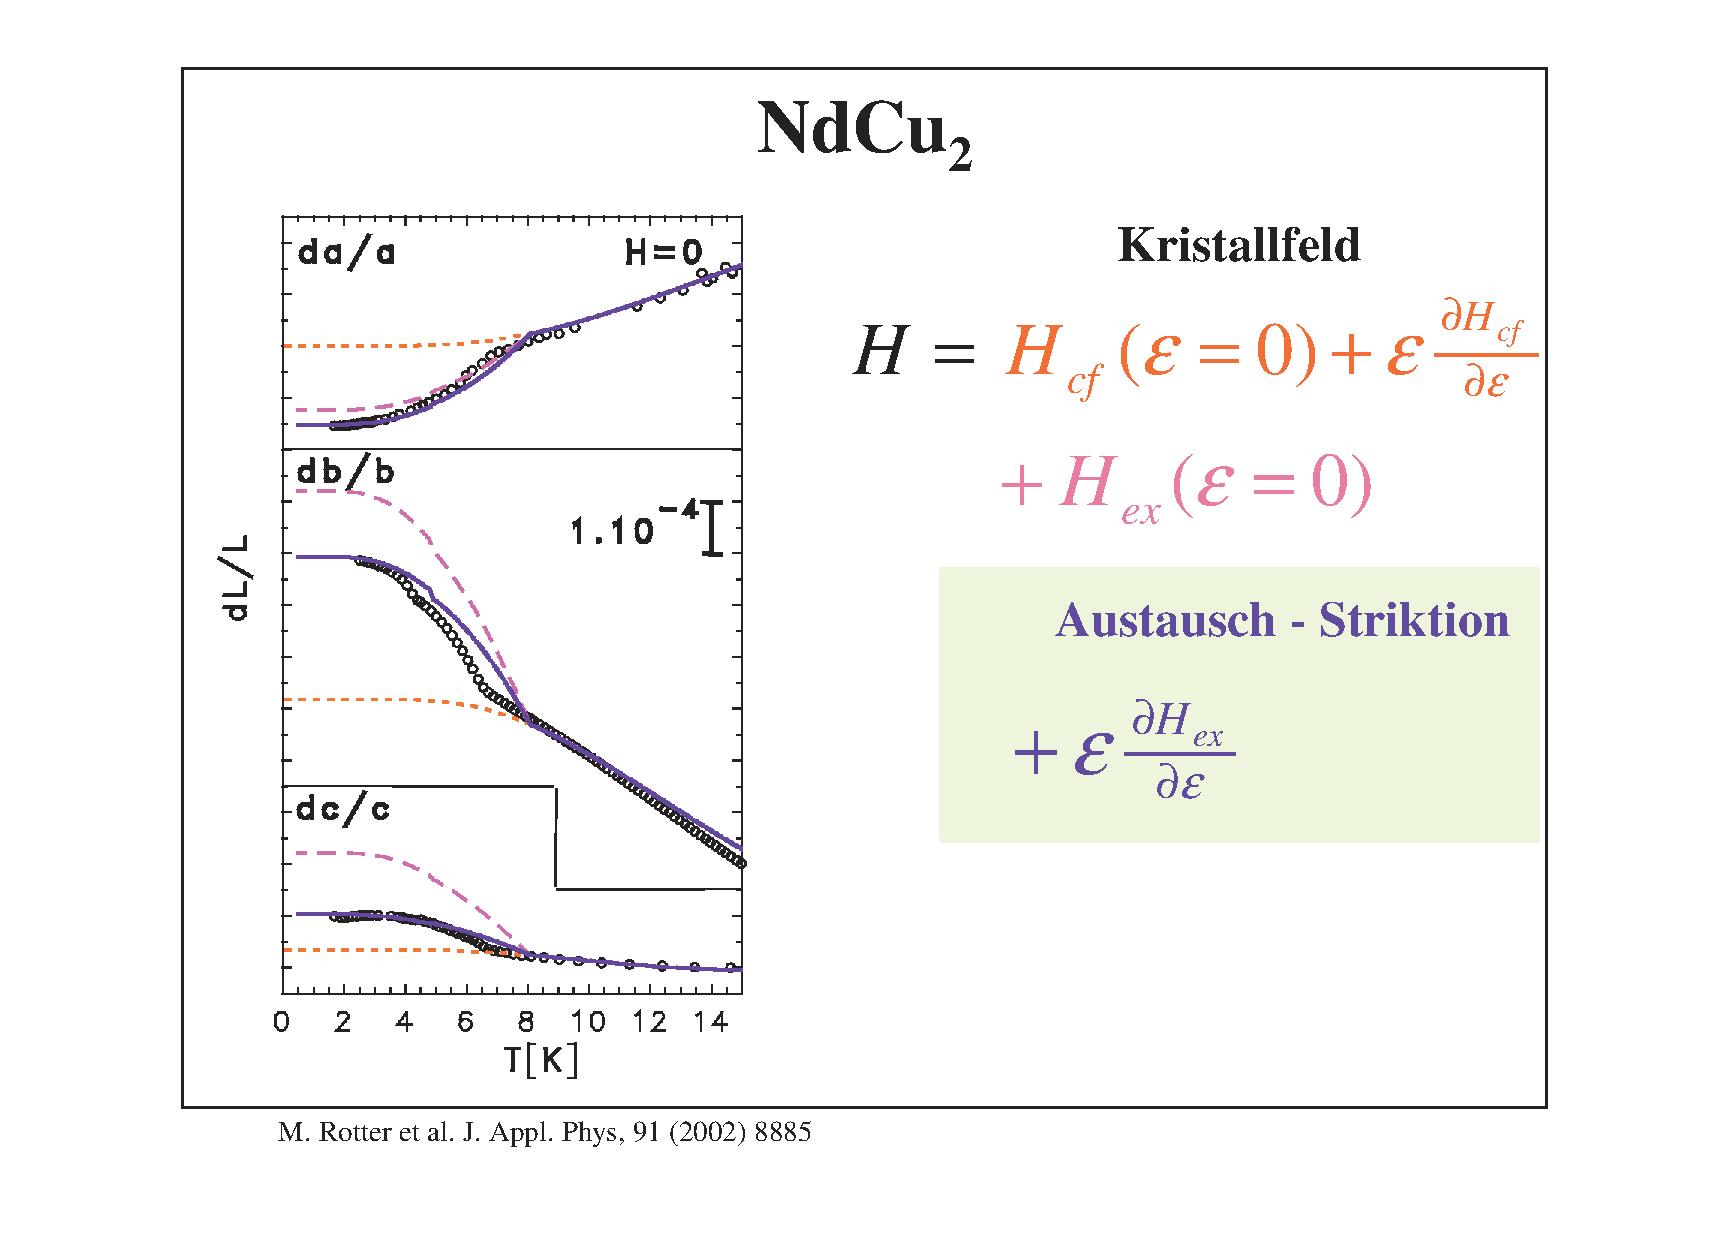
\includegraphics[angle=0, width=0.8\textwidth]{figsrc/magnetostriction_ndcu2.eps}
\end{center}
\caption{Calculated spontaneous magnetostriction of NdCu$_2$.}
\label{magnetostrictiongraphic}
\end{figure}

\begin{description}
\item [\prg mcphas.qvc]    the set of test q-vectors used for calculation of free energy.
                           Components of these q vectors refer to the reciprocal lattice $\vec a^*,\vec b^*,\vec c^*$.
\item [\prg mcphas.phs]    spin-configuration table of different types of spin-configurations. 
                            Note, in case of non-orthogonal axes the convention in these tables 
                            is $mb||\vec b$, $mc||(\vec a \times \vec b)$ and $ma$ perpendicular to $mb$ and $mc$.

                           {\em Note}: 
                           there is no natural criteria for deciding, if one spin-configuration is
			   different from another one. Therefore the list of ''different''
			   spin-configurations is dependent on the meaning of ''different''.
			   
			   The program {\prg McPhase} decides whether a spin-configuration is
			   different from another by a simple criteria, namely by the
			   angle between the spins. Comparing two spin configurations it calculates
			   the angle between corresponding spins and if for one spin the
			   angle is not small, the configuration is treated as a different
			   configuration. Therefore for example a ferromagnet with moments
			   in $a$ has a different spin configuration than a ferromagnet with
			   moments in $b$ direction. 
\item [\prg mcphas.sps]    $T-H$ dependence of spin-configuration. The spin configurations stored in this
                           file may be displayed using the program {\prg spins\index{spins}}, an example is given
			   in figure~\ref{spingraphic}.
                            Note, in case of non-orthogonal axes the convention for applied field $Ha, Hb,Hc$ and
                            also for the moment components $ma, mb, mc$ in these tables 
                            is $mb||\vec b$, $mc||(\vec a \times \vec b)$ and $ma$ perpendicular to $mb$ and $mc$.

\item [\prg mcphas.mf]     $T-H$ dependence of exchange field configuration, stored as $g_J \mu_B H_{xc}(i)$(unit is in meV)
                            for i=1,2,...,number of spins in magnetic unit cell.
                            Note, in case of non-orthogonal axes the convention for applied field $Ha, Hb,Hc$ and
                            also for the mean field components in these tables 
                            is $Hb||\vec b$, $Hc||(\vec a \times \vec b)$ and $Ha$ perpendicular to $Hb$ and $Hc$.
\item [\prg mcphas.fum]    free energy, magnetic energy (the derivative with respect to temperature gives the specific %%@
heat),
                           magnetisation data and (if cfield is used with higher order interactions)
                           expectation values of the Stevens Operators $<O_l^m>$ . As an example for the information
			   contained in this file the calculated magnetisation and magnetostriction of NdCu$_2$ is shown in
			   figures~\ref{magnetization} and ~\ref{magnetizationgraphic}.
                            Note, in case of non-orthogonal axes the convention for applied field $Ha, Hb,Hc$ and
                            also for the magnetisation components $ma,mb,mc$ in these tables 
                            is $Hb||\vec b$, $Hc||(\vec a \times \vec b)$ and $Ha$ perpendicular to $Hb$ and $Hc$.

\item [\prg mcphas1.j1 .j1 .j2 ...] 
               spin-spin correlation functions for sub-lattice 1 neighbour 1 2 ...
	       (linear combination is proportional to magnetostriction)
	       The spin-spin correlation functions for neighbour $k$ are defined by
	       the following sum of dyadic products:

	       \begin{equation}
	        \frac{1}{n}\sum_{s=1}^n <{\mbf J}^s> \times  <{\mbf J}^{s+k}>
	       \end{equation}
	       with $n$ being the number of moments in the magnetic unit cell.
	       Single ion and two-ion magnetostriction can be calculated using the $<O_l^m>$ and the
	       spin-spin correlation functions. As an example the magnetostriction analysis of
	       NdCu$_2$ is shown in figure~\ref{magnetostrictiongraphic}. For details 
             please refer to~\cite{rotter02-8885}.
                            Note, in case of non-orthogonal axes the convention for applied field $Ha, Hb,Hc$ and
                            also for the moment components in these tables 
                            is $Hb||\vec b$, $Hc||(\vec a \times \vec b)$ and $Ha$ perpendicular to $Hb$ and $Hc$.
\item [\prg mcphas.xyt]    phase diagram as x,y,T, H, phase-number j according to spin-configuration table
               given in mcphas.phs, a periodicity key, nettomoments <J>.
 Figure~\ref{phasediagramgraphic}
	       shows the phase diagram of NdCu$_2$ for magnetic fields parallel to the orthorhombic $b$-direction.
                            Note, in case of non-orthogonal axes the convention for applied field $Ha, Hb,Hc$ 
                             in these tables 
                            is $Hb||\vec b$, $Hc||(\vec a \times \vec b)$ and $Ha$ perpendicular to $Hb$ and $Hc$.
\item [\prg mcphas.hkl]    calculated (unpolarised) neutron diffraction data (the calculated magnetic intensities
    correspond to the magnetic structure + Polarisation factor. The
    Lorentz-factor , magnetic form factor and  instrumental corrections are not calculated.)
 As an example figure~\ref{neutintgraphic}
    shows the calculated temperature dependence of magnetic amplitudes for NdCu$_2$.
                           $h,k,l$ refer to the reciprocal lattice $\vec a^*,\vec b^*,\vec c^*$.
                            Note, in case of non-orthogonal axes the convention for applied field $Ha, Hb,Hc$ 
                             in these tables 
                            is $Hb||\vec b$, $Hc||(\vec a \times \vec b)$ and $Ha$ perpendicular to $Hb$ and $Hc$.
    
\item [\prg mcphasa.hkl]    Fourier Transform of the $a$-component of the magnetic Moments.
                           $h,k,l$ refer to the reciprocal lattice $\vec a^*,\vec b^*,\vec c^*$.
                            Note, in case of non-orthogonal axes the convention for applied field $Ha, Hb,Hc$ and
                            the magnetic moment component in these tables 
                            is $Hb||\vec b$, $Hc||(\vec a \times \vec b)$ and $Ha$ perpendicular to $Hb$ and $Hc$.
\item [\prg mcphasb.hkl]    Fourier Transform of the $b$-component of the magnetic Moments.
                           $h,k,l$ refer to the reciprocal lattice $\vec a^*,\vec b^*,\vec c^*$.
                            Note, in case of non-orthogonal axes the convention for applied field $Ha, Hb,Hc$ and
                            the magnetic moment component in these tables 
                            is $Hb||\vec b$, $Hc||(\vec a \times \vec b)$ and $Ha$ perpendicular to $Hb$ and $Hc$.
\item [\prg mcphasc.hkl]    Fourier Transform of the $c$-component of the magnetic Moments.
                           $h,k,l$ refer to the reciprocal lattice $\vec a^*,\vec b^*,\vec c^*$.
                            Note, in case of non-orthogonal axes the convention for applied field $Ha, Hb,Hc$ and
                            the magnetic moment component in these tables 
                            is $Hb||\vec b$, $Hc||(\vec a \times \vec b)$ and $Ha$ perpendicular to $Hb$ and $Hc$.
\end{description} 

\vspace{1cm}
{\em Exercises:}
\begin{itemize}
\item Look at the output files of {\prg McPhase}  in the directory
{\prg examples/ndcu2b\_new/results}.  At which magnetic field
the ferromagnetically aligned state is achieved (at $T=$2~K)?
\item
What is the propagation vector in the different antiferromagnetic phases at $T=$2~K ?
\end{itemize}



\subsubsection{{\prg mcphas.tst\index{mcphas.tst}} - input file of test spin-configurations (optional)}
This file is optional and contains
some test momentum configurations to be used for the calculation
             of the free energy. Mind that
\begin{itemize}
\item  in the file header the number of atoms in the primitive
       crystallographic unit cell and the number of components
       of the spin vector have to be given.
\item  at the end of the
 file there must be no empty lines !
\end{itemize}

The momentum - configurations tables always refer to spins sitting on
the primitive lattice ${\mbf r}_i$. If more than one atom is in
the primitive basis, the momentum gets $3n$ components ($n=$ number
of atoms in the crystallographic basis). See {\prg ./examples/ndcu2b\_new/} for
examples of a two atom basis. Units of these tables are that of total 
angular momentum $<J>$.

\subsubsection{Example {\prg mcphas.tst\index{mcphas.tst}} file  for a simple antiferromagnet}

Here is the file {\prg mcphas.tst\index{mcphas.tst}} for the simple antiferromagnet example
describing some spin configurations
to be used as starting values for the mean field process:

\section{{\prg mcphas} - calculation of thermodynamic properties (Magnetisation, Susceptibility, Specific Heat, Neutron %%@
Diffraction, etc.)}
\label{runmcphas}

In order to perform calculations beyond the capabilities of {\prg cfield\index{cfield}} it is necessary
to use the program {\prg mcphas}. 
\begin{itemize}
\item As a first step it is possible to
calculate the thermodynamic properties such as magnetisation or specific heat
considering only single ion effects. In this case all the exchange parameters
have to be set to zero in {\prg mcphas.j\index{mcphas.j}}. 
\item for more advanced calculations the two - ion interactions have to be
considered and may lead to magnetic order. {\prg mcphas} can perform 
calculations in the ordered state in the following way: for 
a given temperature $T$ and magnetic field $\mbf H$ (vector)
several possible magnetic structures are stabilised
by a mean field algorithm and the free energy is 
calculated. The initial values for this mean-field procedure are
modified by a Monte Carlo process.


The temperature and magnetic field is varied during the calculation
and thereby it is possible to map out the magnetic phase diagram.
\end{itemize}

The program produces a plot of the stabilised magnetic
structures and the magnetisation on screen, the
output files contain additional information 
such as calculated magnetoelastic and  neutron-scattering
data. Several graphic programs easy the visualisation of the
calculated data (section~\ref{graphics}).



\subsection{Input Files}
The program {\prg McPhase} needs the following input files (all in the same directory)
 in order to run:

\begin{enumerate}
\item {\prg mcphas.ini\index{mcphas.ini}}
 - controlling the algorithm
\item {\prg mcphas.j\index{mcphas.j}}
  - lattice and exchange parameters
\item {\prg mcphas.tst\index{mcphas.tst}(optional)}  - test spin configurations
\item {\prg single-ion property files}
\item {\prg directory ./results/}
 - directory where calculated data is stored
\item {\prg directory ./fit} - experimental data for fit (optional)
\end{enumerate}


 All
 of these input files have to be in one directory and the program
has to be started in this directory. The results of the simulation
are then stored in the  subdirectory ./results/, which must exist before starting
the program 
... see directory ./examples/ for some examples.
 In order to prepare these files
for a new calculation it is best to take them from an example, copy the files
to a new directory and make the
modifications  to adapt them to the new problem.

\subsubsection{Example - a simple antiferromagnet}

In the following description of the input files we will always refer
to a simple example: a simple antiferromagnet
on a primitive orthorhombic lattice. The first time user
will thus have a simple example to follow, all corresponding
files are given in the directory {\prg tutorial/03magnetic\_phases\_mcphas/simpleAF}.
 

\subsubsection{{\prg mcphas.ini\index{mcphas.ini}} - controlling the algorithm}
   Initial file containing algorithm control parameters, for instance the range and spacing of
   propagation vectors Q or the number of Monte Carlo trials for initial spin configurations
    - {\em mind}: this
   file is rewritten and reread  when running the program and may be changed by the
   user in order to manipulate the running simulation.

{\prg mcphas.ini\index{mcphas.ini}} consists of several sections:
\begin{description}
\item [MCPHASE RUNTIME CONTROL:] this section contains the parameters
controlling the status of the calculation.
\item [XY PHASEDIAGRAM PARAMETERS:] here the temperature and field range and
step widths of the calculation are specified.
The definition of the x and y
axis in terms of temperature and magnetic field is followed by the
corresponding range and step width. An offset may be given for all
field and temperature values.
Note that for most cases of interest
this offset is zero (T0=0, Ha0=0, Hb0=0, Hc0=0).
 For the simple case of calculating a Temperature-Field phase diagram
 It is just necessary to set xT=1 and give the temperature range by
xmin/xmax/xstep. For field in b direction then just set yHb=1 and 
define the range in ymin/ymax/ystep.
In case of non-orthogonal axes the applied magnetic field
components $Ha, Hb, Hc$ refer to the orthogonal coordinate system
defined with respect to the nonorthogonal lattice $\mbf a,\mbf b,\mbf c$ as
$Hb||\mbf b$, $Hc||(\mbf a \times \mbf b)$ and $Ha$ perpendicular to $Hb$ and $Hc$.

\item [GENERATION OF SPINCONFIGURATIONS:] at the beginning of the program
some initial values of spin configurations are generated from a set of 
propagation vectors. This section defines the range of propagation vectors
and the step width.
Depending on the value of the propagation Q with respect to the primitive reciprocal lattice
1-, 2- or 3-dimensional simulations of magnetic lattices
are possible. It is advisable to 
think carefully about the chosen range and spacing of Q vectors in order
to limit calculation time.
 
For example a good starting point is to begin with a calculation with large
step widths (e.g. 0.1)  covering the Brillouin zone. This should give an idea
of the propagation vectors which are stabilised. An advanced calculation
could then fine tune the propagation and determine its accurate value (using
small step widths in a limited area of the zone).
The verbose option of {\prg mcphas} allows to inspect the propagation vectors
which are actually used in the calculation.
Trick: in order to get a quick overview of the
q-vector range covered by the mcphas\index{mcphas} simulation start mcphas, exit and 
just type {\prg felog ./results/mcphas.qvc} (need {\prg perl,perldl,pdl,pgplot} packages).

In order to limit calculation time, the maximum periodicity
of the magnetic unit cell with respect to the crystallographic unit cell 
(maxqperiod) and the maximum number of spins in the magnetic unit cell 
(maxnofspins) can be limited. Also the maximum number of test spin configurations
in the internal table can be limited (maxnoftestspincf).
A critical feature with respect to calculation time is also the number of
spin configurations which are generated by a random process from a tabulated
SPINCONFIGURATIONS during the calculation. 

In summary the variables in this section are mainly important to adapt the
program to a given computer system with finite speed. They have to be set
to optimise between speed and accuracy of the calculation. In order to
find appropriate values it is best to perform some calculations 
and restrict the parameters step by step if insufficient speed is obtained.
Also the examples included in the program package may serve as starting
points.

\item [PARAMETERS FOR SUB FECALC SELFCONSISTENCY PROCESS:] the most important
procedure in the module {\prg mcphas} is the sub fecalc. In this part of the 
program the self consistent calculation of the magnetic moment configuration
is performed as shown schematically in fig.~\ref{fecalc}. 
In the mean field approximation the Hamiltonian~(\ref{hamilton}) is approximated
by

\begin{equation}
 {\mathcal H}=\sum_n H_{SI}^n + E_{corr}
\end{equation}

with the single ion Hamiltonian (in case of module {\prg so1ion\index{so1ion}})

\begin{equation}
H_{SI}^n=  B_l^m O_{lm}({\mbf J}^n) 
	     - g_{Jn} \mu_B {\mbf J}^n {\mbf H^n_{eff}} 
\end{equation}

and the correction term

\begin{equation}
E_{corr}=\frac{1}{2}\sum_{n} g_{Jn} \mu_B \langle {\mbf J}^n
 \rangle (\mbf H^n_{eff}-\mbf H) 
\end{equation}

and with the mean fields $ \mbf H^n_{eff}$ given by

\begin{equation}\label{meanfield}
\mbf H^n_{eff}=\mbf H + \mbf H^n_{xc}=\mbf H+\sum_{{\mbf G'}n'} \frac{{\mathcal J}
(\mbf r_n-(\mbf G'+\mbf r_{n'}))}{g_{Jn}\mu_B } \langle{\mbf
J}^{n'}\rangle
\end{equation}

These mean fields and the moments $\langle \mbf J^n \rangle$ 
are determined in a self consistent
way. For a given magnetic unit cell and initial configuration 
of magnetic moments
the mean fields are calculated according to equation~(\ref{meanfield}). 
Then, for each
magnetic ion the single ion property module is taken 
and the magnetic moment $\langle \mbf J^n \rangle$ is 
calculated from it's mean field. The mean fields are used again in equation~(\ref{meanfield})
and so on .... until convergence is reached. 
Then, the free energy ($f=-kT\sum_n \ln(z_n) + E_{corr}$ ) 
of the stabilised
configuration is calculated (this is why this sub is called {\prg fecalc}). 
The free energies of a lot of different stabilised configurations have to
be compared in order to find out which configuration has lowest free energy, i.e.
is stable in thermal  equilibrium.

It may happen that this process does
not converge due to bad choice of the initial configuration, therefore a maximum number
of mean field loops has to be given by the user.
The results of a calculation may be significantly influenced by
changing parameters such as the maximum number of iteration loops 
in this section. 
In fact the simulation is always a compromise of calculation time and accuracy: if only
a few initial spin configurations are tried at each (H-T) point, the calculation speed is
fast, however it is possible that the program misses the magnetic structure with the
lowest free energy. The same holds if other critical parameters of the simulation are
restricted too much.
 

\item [OUTPUT OF PHYSICAL PROPERTIES:]
Some options for the output of the calculation can be changed in this section.
\end{description}

\begin{figure}[hb]
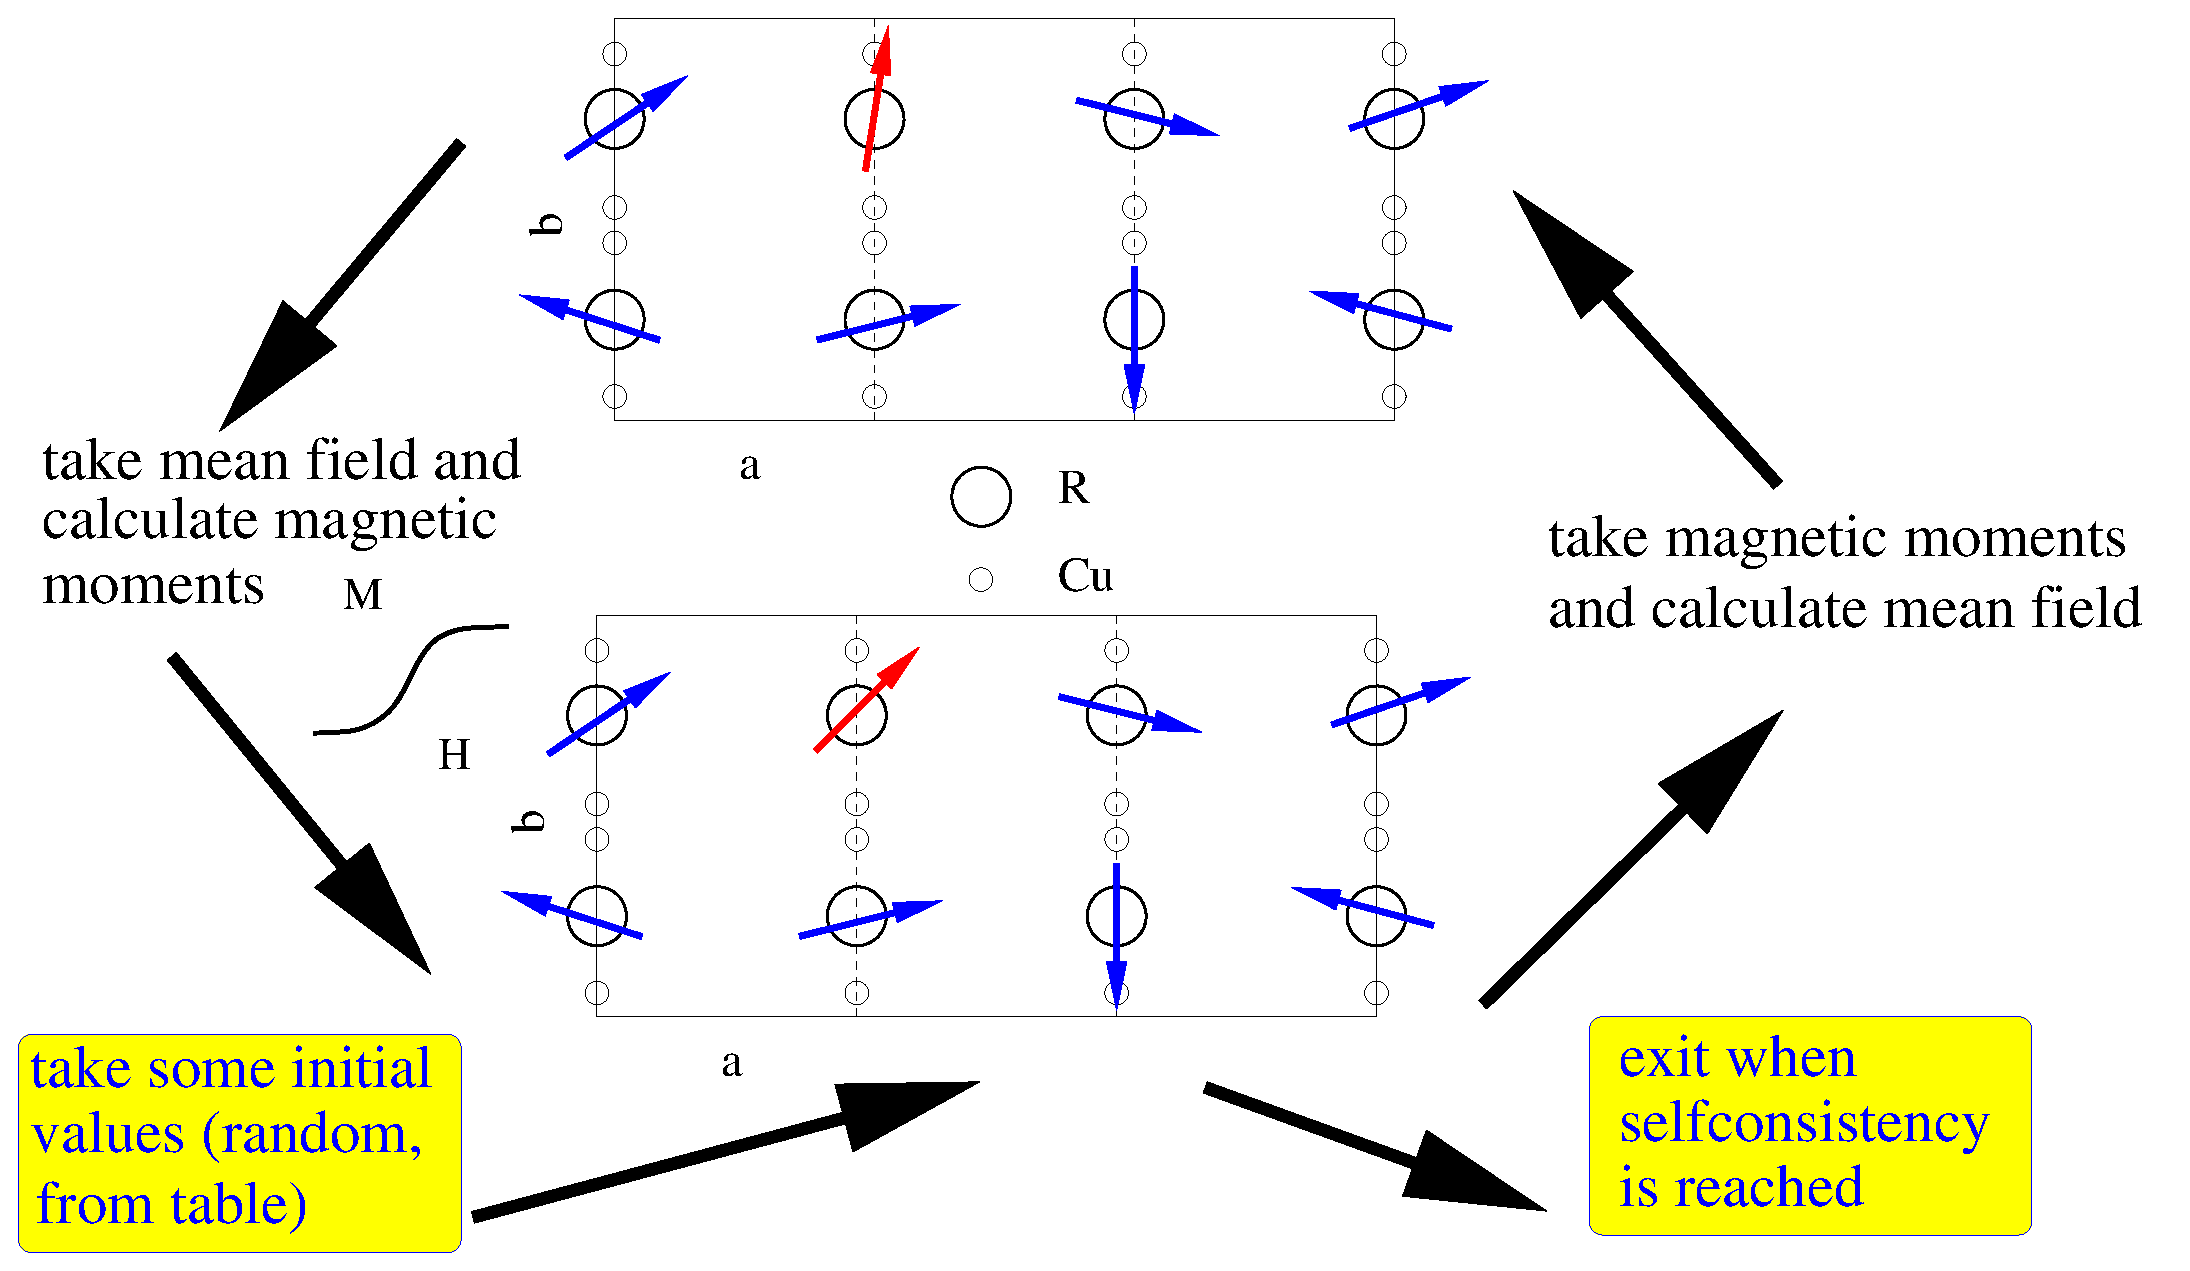
\includegraphics[angle=0,width=0.9\columnwidth]{figsrc/fecalc.eps}
\caption{\label{fecalc}Mean field process of sub {\prg fecalc}.}
\end{figure}

 
\subsubsection{Example {\prg mcphas.ini\index{mcphas.ini}} file for a simple antiferromagnet}

Here is an example of {\prg mcphas.ini\index{mcphas.ini}}, the comments describe the meaning of the different
parameters:

\section{{\prg mcphas} - calculation of thermodynamic properties (Magnetisation, Susceptibility, Specific Heat, Neutron %%@
Diffraction, etc.)}
\label{runmcphas}

In order to perform calculations beyond the capabilities of {\prg cfield\index{cfield}} it is necessary
to use the program {\prg mcphas}. 
\begin{itemize}
\item As a first step it is possible to
calculate the thermodynamic properties such as magnetisation or specific heat
considering only single ion effects. In this case all the exchange parameters
have to be set to zero in {\prg mcphas.j\index{mcphas.j}}. 
\item for more advanced calculations the two - ion interactions have to be
considered and may lead to magnetic order. {\prg mcphas} can perform 
calculations in the ordered state in the following way: for 
a given temperature $T$ and magnetic field $\mbf H$ (vector)
several possible magnetic structures are stabilised
by a mean field algorithm and the free energy is 
calculated. The initial values for this mean-field procedure are
modified by a Monte Carlo process.


The temperature and magnetic field is varied during the calculation
and thereby it is possible to map out the magnetic phase diagram.
\end{itemize}

The program produces a plot of the stabilised magnetic
structures and the magnetisation on screen, the
output files contain additional information 
such as calculated magnetoelastic and  neutron-scattering
data. Several graphic programs easy the visualisation of the
calculated data (section~\ref{graphics}).



\subsection{Input Files}
The program {\prg McPhase} needs the following input files (all in the same directory)
 in order to run:

\begin{enumerate}
\item {\prg mcphas.ini\index{mcphas.ini}}
 - controlling the algorithm
\item {\prg mcphas.j\index{mcphas.j}}
  - lattice and exchange parameters
\item {\prg mcphas.tst\index{mcphas.tst}(optional)}  - test spin configurations
\item {\prg single-ion property files}
\item {\prg directory ./results/}
 - directory where calculated data is stored
\item {\prg directory ./fit} - experimental data for fit (optional)
\end{enumerate}


 All
 of these input files have to be in one directory and the program
has to be started in this directory. The results of the simulation
are then stored in the  subdirectory ./results/, which must exist before starting
the program 
... see directory ./examples/ for some examples.
 In order to prepare these files
for a new calculation it is best to take them from an example, copy the files
to a new directory and make the
modifications  to adapt them to the new problem.

\subsubsection{Example - a simple antiferromagnet}

In the following description of the input files we will always refer
to a simple example: a simple antiferromagnet
on a primitive orthorhombic lattice. The first time user
will thus have a simple example to follow, all corresponding
files are given in the directory {\prg tutorial/03magnetic\_phases\_mcphas/simpleAF}.
 

\subsubsection{{\prg mcphas.ini\index{mcphas.ini}} - controlling the algorithm}
   Initial file containing algorithm control parameters, for instance the range and spacing of
   propagation vectors Q or the number of Monte Carlo trials for initial spin configurations
    - {\em mind}: this
   file is rewritten and reread  when running the program and may be changed by the
   user in order to manipulate the running simulation.

{\prg mcphas.ini\index{mcphas.ini}} consists of several sections:
\begin{description}
\item [MCPHASE RUNTIME CONTROL:] this section contains the parameters
controlling the status of the calculation.
\item [XY PHASEDIAGRAM PARAMETERS:] here the temperature and field range and
step widths of the calculation are specified.
The definition of the x and y
axis in terms of temperature and magnetic field is followed by the
corresponding range and step width. An offset may be given for all
field and temperature values.
Note that for most cases of interest
this offset is zero (T0=0, Ha0=0, Hb0=0, Hc0=0).
 For the simple case of calculating a Temperature-Field phase diagram
 It is just necessary to set xT=1 and give the temperature range by
xmin/xmax/xstep. For field in b direction then just set yHb=1 and 
define the range in ymin/ymax/ystep.
In case of non-orthogonal axes the applied magnetic field
components $Ha, Hb, Hc$ refer to the orthogonal coordinate system
defined with respect to the nonorthogonal lattice $\mbf a,\mbf b,\mbf c$ as
$Hb||\mbf b$, $Hc||(\mbf a \times \mbf b)$ and $Ha$ perpendicular to $Hb$ and $Hc$.

\item [GENERATION OF SPINCONFIGURATIONS:] at the beginning of the program
some initial values of spin configurations are generated from a set of 
propagation vectors. This section defines the range of propagation vectors
and the step width.
Depending on the value of the propagation Q with respect to the primitive reciprocal lattice
1-, 2- or 3-dimensional simulations of magnetic lattices
are possible. It is advisable to 
think carefully about the chosen range and spacing of Q vectors in order
to limit calculation time.
 
For example a good starting point is to begin with a calculation with large
step widths (e.g. 0.1)  covering the Brillouin zone. This should give an idea
of the propagation vectors which are stabilised. An advanced calculation
could then fine tune the propagation and determine its accurate value (using
small step widths in a limited area of the zone).
The verbose option of {\prg mcphas} allows to inspect the propagation vectors
which are actually used in the calculation.
Trick: in order to get a quick overview of the
q-vector range covered by the mcphas\index{mcphas} simulation start mcphas, exit and 
just type {\prg felog ./results/mcphas.qvc} (need {\prg perl,perldl,pdl,pgplot} packages).

In order to limit calculation time, the maximum periodicity
of the magnetic unit cell with respect to the crystallographic unit cell 
(maxqperiod) and the maximum number of spins in the magnetic unit cell 
(maxnofspins) can be limited. Also the maximum number of test spin configurations
in the internal table can be limited (maxnoftestspincf).
A critical feature with respect to calculation time is also the number of
spin configurations which are generated by a random process from a tabulated
SPINCONFIGURATIONS during the calculation. 

In summary the variables in this section are mainly important to adapt the
program to a given computer system with finite speed. They have to be set
to optimise between speed and accuracy of the calculation. In order to
find appropriate values it is best to perform some calculations 
and restrict the parameters step by step if insufficient speed is obtained.
Also the examples included in the program package may serve as starting
points.

\item [PARAMETERS FOR SUB FECALC SELFCONSISTENCY PROCESS:] the most important
procedure in the module {\prg mcphas} is the sub fecalc. In this part of the 
program the self consistent calculation of the magnetic moment configuration
is performed as shown schematically in fig.~\ref{fecalc}. 
In the mean field approximation the Hamiltonian~(\ref{hamilton}) is approximated
by

\begin{equation}
 {\mathcal H}=\sum_n H_{SI}^n + E_{corr}
\end{equation}

with the single ion Hamiltonian (in case of module {\prg so1ion\index{so1ion}})

\begin{equation}
H_{SI}^n=  B_l^m O_{lm}({\mbf J}^n) 
	     - g_{Jn} \mu_B {\mbf J}^n {\mbf H^n_{eff}} 
\end{equation}

and the correction term

\begin{equation}
E_{corr}=\frac{1}{2}\sum_{n} g_{Jn} \mu_B \langle {\mbf J}^n
 \rangle (\mbf H^n_{eff}-\mbf H) 
\end{equation}

and with the mean fields $ \mbf H^n_{eff}$ given by

\begin{equation}\label{meanfield}
\mbf H^n_{eff}=\mbf H + \mbf H^n_{xc}=\mbf H+\sum_{{\mbf G'}n'} \frac{{\mathcal J}
(\mbf r_n-(\mbf G'+\mbf r_{n'}))}{g_{Jn}\mu_B } \langle{\mbf
J}^{n'}\rangle
\end{equation}

These mean fields and the moments $\langle \mbf J^n \rangle$ 
are determined in a self consistent
way. For a given magnetic unit cell and initial configuration 
of magnetic moments
the mean fields are calculated according to equation~(\ref{meanfield}). 
Then, for each
magnetic ion the single ion property module is taken 
and the magnetic moment $\langle \mbf J^n \rangle$ is 
calculated from it's mean field. The mean fields are used again in equation~(\ref{meanfield})
and so on .... until convergence is reached. 
Then, the free energy ($f=-kT\sum_n \ln(z_n) + E_{corr}$ ) 
of the stabilised
configuration is calculated (this is why this sub is called {\prg fecalc}). 
The free energies of a lot of different stabilised configurations have to
be compared in order to find out which configuration has lowest free energy, i.e.
is stable in thermal  equilibrium.

It may happen that this process does
not converge due to bad choice of the initial configuration, therefore a maximum number
of mean field loops has to be given by the user.
The results of a calculation may be significantly influenced by
changing parameters such as the maximum number of iteration loops 
in this section. 
In fact the simulation is always a compromise of calculation time and accuracy: if only
a few initial spin configurations are tried at each (H-T) point, the calculation speed is
fast, however it is possible that the program misses the magnetic structure with the
lowest free energy. The same holds if other critical parameters of the simulation are
restricted too much.
 

\item [OUTPUT OF PHYSICAL PROPERTIES:]
Some options for the output of the calculation can be changed in this section.
\end{description}

\begin{figure}[hb]
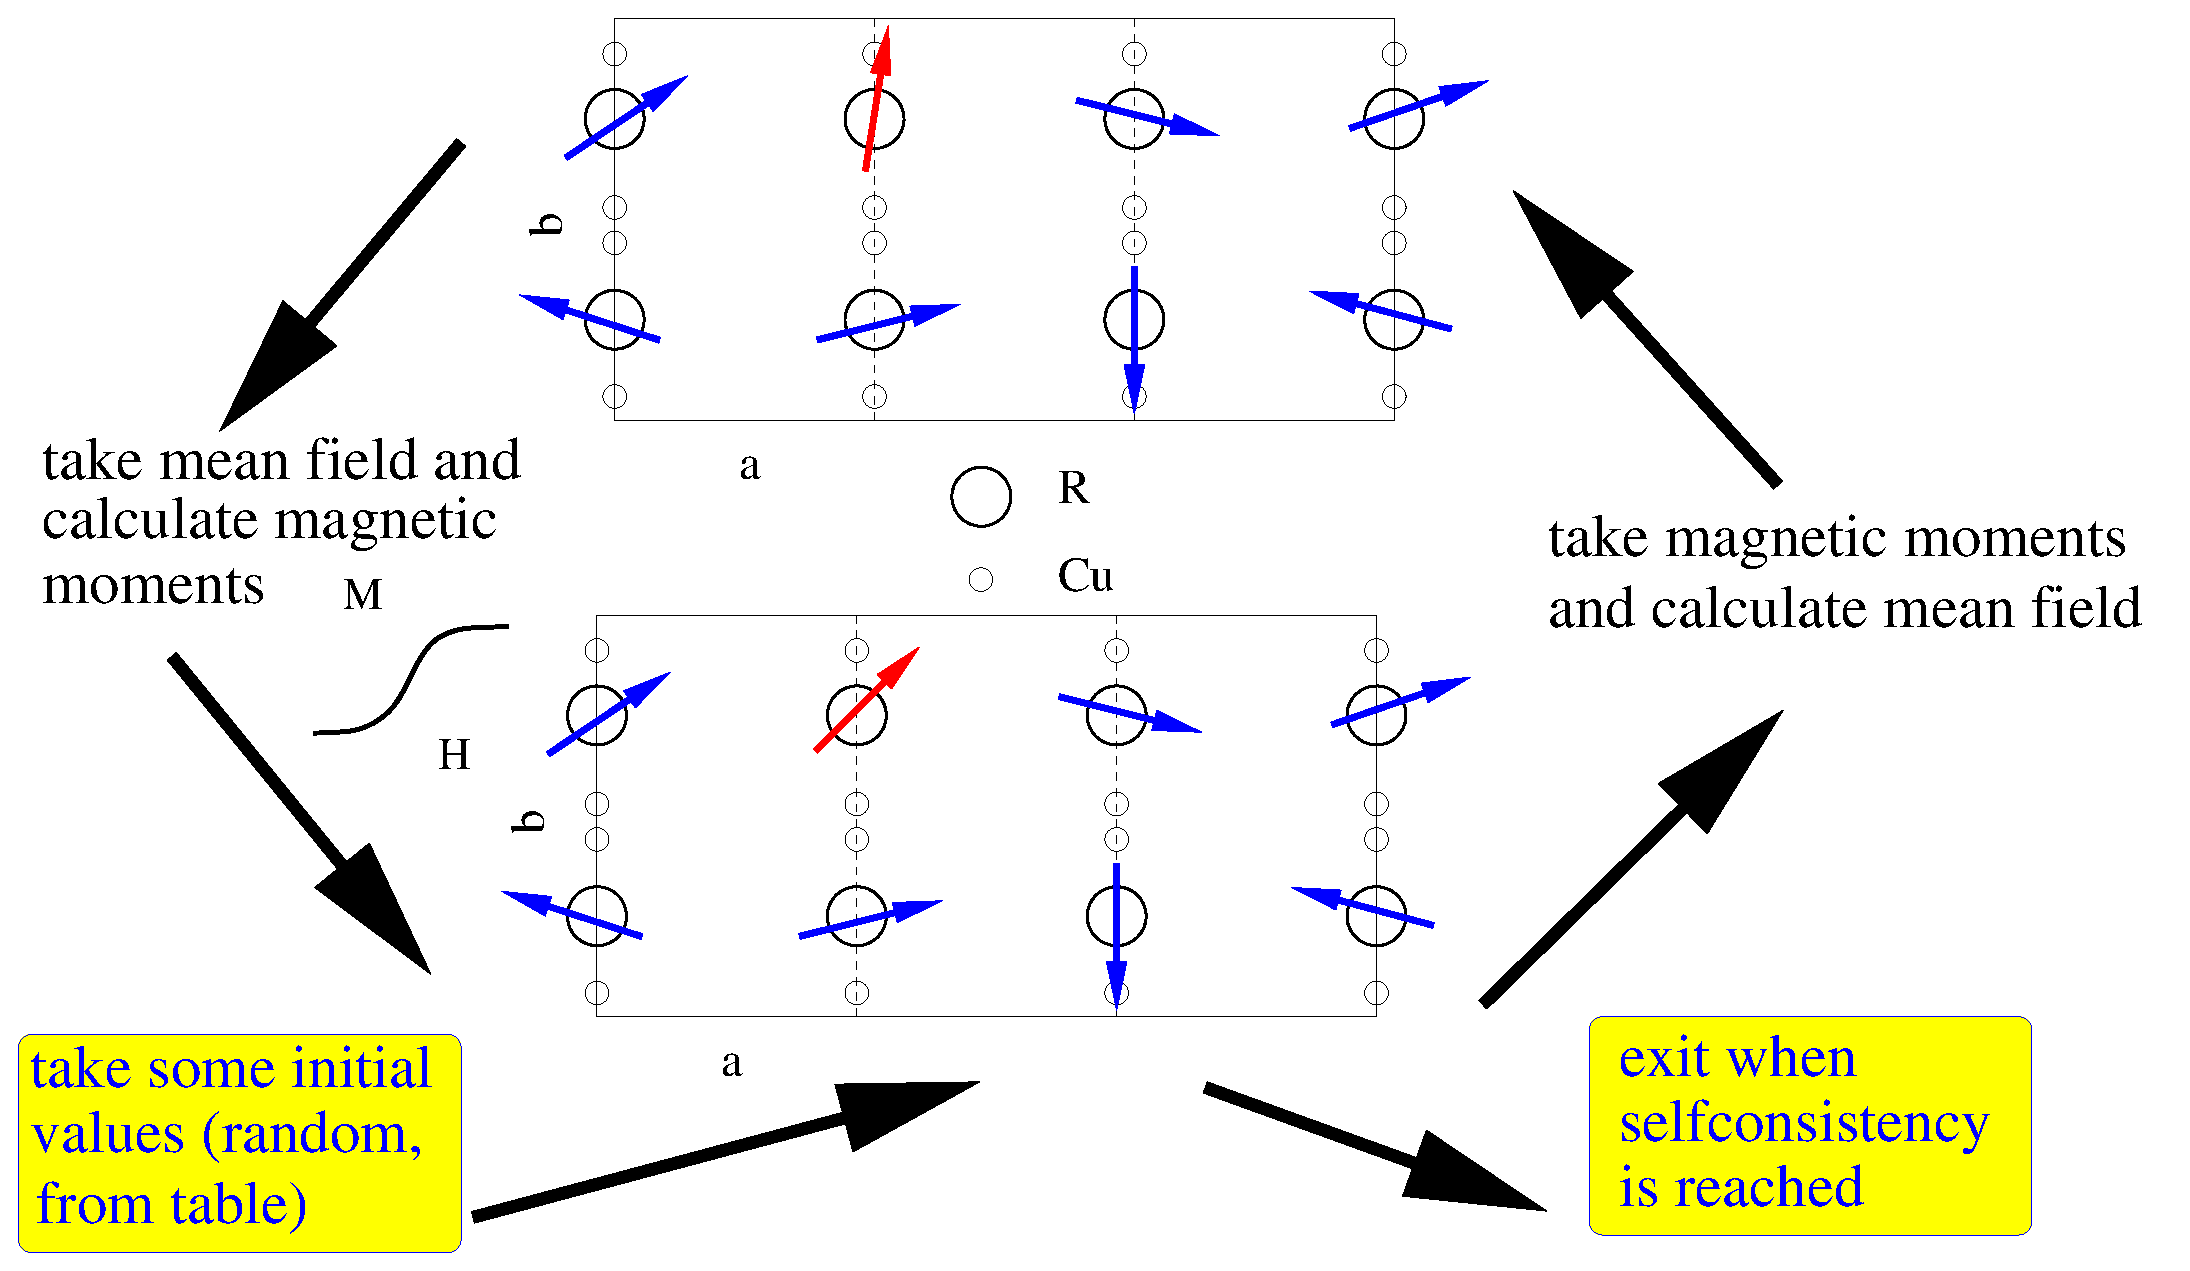
\includegraphics[angle=0,width=0.9\columnwidth]{figsrc/fecalc.eps}
\caption{\label{fecalc}Mean field process of sub {\prg fecalc}.}
\end{figure}

 
\subsubsection{Example {\prg mcphas.ini\index{mcphas.ini}} file for a simple antiferromagnet}

Here is an example of {\prg mcphas.ini\index{mcphas.ini}}, the comments describe the meaning of the different
parameters:

\input{mcphas.ini}



\subsubsection{{\prg mcphas.j\index{mcphas.j}} - lattice and exchange parameters}\label{mcphasj}
This file provides the information about 
the crystallographic
 structure and the magnetic exchange interactions.
For every atom in the crystallographic basis there
has to be given the coordinates, the number of neighbours to be considered, the 
Land\'e factor $g_J$, the single ion property filename and  a set of exchange parameters.
If the exchange parameters (and neighbour positions) are not known for your system, you 
can use the program module {\prg makenn\index{makenn}} (see section \ref{addprog}) to generate 
a list of nearest neighbours and
exchange parameters, currently implemented in {\prg makenn\index{makenn}} are dipolar interactions,
exchange interactions via the Bethe-Slater curve or the RKKY model. Note that in order
to use {\prg makenn\index{makenn}} you have to set up a working {\prg mcphas.j\index{mcphas.j}} file, which may or
may not contain neighbours and interactions.

Use program {\prg addj\index{addj}} to add exchange parameter set stored in different 
such {\prg .j} files (see section~\ref{addprog}).



\begin{description}
\item [Line 1,2:] Comment Lines
\item [Line 3:] lattice constants a,b,c and crystal angles alpha, beta, gamma 
\item [Line 4-6:] primitive lattice vectors
\item [Line 7:] Number of atoms in the primitive crystallographic unit cell ({\prg nofatoms})
\item [Line 8:] a comment line with stars
\item [Line 9:] coordinates  ($d_a$,$d_b$,$d_c$) of 1$^{st}$ magnetic ion in the crystallographic unit cell  with
respect to the lattice vectors $\vec a$,$\vec b$,$\vec c$. The number of neighbours of this 
ion, for which interaction constants are given in the interaction table (nofneighbours). 
If {\prg diagonalexchange}
is set to 0 the 9 components of the exchange tensor are given in column 4-12. 
If {\prg diagonalexchange}
 is 1, only 3 components are given (column 4-6).
If {\prg diagonalexchange}
 is 2, specific components of the exchange tensor can be given in columns 4 onwards. The indices of these components
 must be given in the following line (Line 9a below).
The Land\'e factor of the ion (gJ) and the file name of the corresponding single ion
parameter file (cffilename).
\item [Line 9a:]  If {\prg diagonalexchange=2}, then this line gives the indices of the exchange tensor corresponding to 
 the columns 4 onwards. It must have a variable called {\prg indexexchange} followed by a list of names of components of the interaction
 tensor separated by space. E.g.
 \verb|  #! indexexchange= JaJb JbJc  | 
means column 4 gives the the interaction constant between the
 first angular momentum component of the current ion with the second angular momentum component of its neighbour, whilst 
 column 5 has the interaction constant between the second angular momentum component of this ion with the third component of its
 neighbour. Alternatively, pairs of numbers may be given, as in \verb|  #! indexexchange= 1,2 2,3  |
 Additionally another parameter {\prg symmetricexchange} can be set to 1, where the value in each column is also used 
 for the transposed tensor component. Thus \verb|  #! symmetricexchange=1 indexexchange= JaJb  | is the same as \\
 \verb|  #! indexexchange= JaJb JbJa  | where the 4th and 5th column are the same.
\item [Line 10:]  Comment line
\item [Line 11-(10+nofneighbours):] Interaction table for ion number 1.   
Note: the neighbour coordinates (column 1-3) are given with respect to the lattice vectors
$\vec a$,$\vec b$,$\vec c$. The program then calculates from these values the coordinates
with respect to the primitive lattice $\vec r_1$,~$\vec r_2$,~$\vec r_3$.
($ d_a \vec a + d_b \vec b + d_c \vec c = d_1 \vec r_1 + d_2 \vec r_2 + d_3 \vec r_3$).
Column 4,5,6 \dots contain the components of the interaction tensor $\stackrel{=}{\mathcal J}$. 
Note that in case of non-orthogonal axes the 
components of the moments and the interaction tensor $Ja, Jb, Jc, Jaa, Jbb, Jcc, Jab ...$ 
refer to the orthogonal coordinate system
defined with respect to the nonorthogonal lattice $\vec a,\vec b,\vec c$ as
$Jb||\vec b$, $Jc||(\vec a \times \vec b)$ and $Ja$ perpendicular to $Jb$ and $Jc$.
\item [Line (11+nofneighbours) - end:] for each ion in the unit cell line 8 - (10+nofneighbours)
are repeated.
\end{description}


\vspace{0.5cm}

{\small {\bf Information for experienced users:}
\begin{description}
\item[\prg mcphas.jjj:]
format of exchange parameter file, which only needs a reduced set of exchange
parameters in the input file. Using the program {\prg jjj2j} the file can be transformed
to {\prg mcphas.j\index{mcphas.j}} by adding lines for all the equivalent neighbours. The format definition
of {\prg mcphas.jjj} is the same as {\prg mcphas.j\index{mcphas.j}}, however each line denotes several
equivalent neighbour atoms (instead of only one in {\prg mcphas.j\index{mcphas.j}}) according to the
 following rules:
\begin{itemize}
\item If a nonzero coordinate $d_a$ (or $d_b$,$d_c$) in the interaction table
 corresponds to it's value at the nearest
 lattice point of the primitive lattice,
  additional interactions of the same size
with  neighbours with coordinate $-d_a$ (or $-d_b$,$-d_c$, respectively)
are taken into account. This
holds for each of the three coordinates $d_a$,$d_b$ and $d_c$
 resulting in a maximum
number of 8 equivalent neighbours per line in the interaction table.
\item If the value of $d_a$ (or $d_b$,$d_c$) is zero or differs
from it's value at the nearest lattice point of the primitive lattice, it is 
changed to the value at the nearest lattice point and {\bf no} interaction 
with  neighbours with coordinates $-d_a$ (or $-d_b$,$-d_c$) is
 taken into account. If such
 interaction is needed it may be given in a different line and may
have different magnitude. In this way also crystallographic lattices
with no mirror symmetry may be described.
\end{itemize}
\item[\prg mcphas.coq:]   exchange parameters etc [ in old format]...see examples for details, use {\prg coq2jjj} to 
transform {\prg mcphas.coq} to {\prg mcphas.jjj} format
\end{description}

}


\subsubsection{Example {\prg mcphas.j\index{mcphas.j}} file for a simple antiferromagnet}

Here are example files of a tetragonal antiferromagnet with nearest neighbour interactions, all
files are equivalent:

{\small
\begin{verbatim} 
# simple antiferromagnet 
#<!--mcphase.mcphas.j-->
#***************************************************************
# Lattice Constants (A)
#! a=4.3843 b=4.3843 c=2.4194 alpha=  90 beta=  90 gamma=  90
#! r1a=   1 r2a=   0 r3a=   0
#! r1b=   0 r2b=   1 r3b=   0   primitive lattice vectors [a][b][c]
#! r1c=   0 r2c=   0 r3c=   1
#! nofatoms=1  nofcomponents=3  number of atoms in primitive unit cell/number of components of each spin
# ****************************************************************************
#! da=  0 [a] db=  0 [b] dc=  0 nofneighbours=2 diagonalexchange=0 gJ=0.857143 cffilename=Ce3p.sipf
# da[a] db[b] dc[c] Jaa[meV] Jbb[meV] Jcc[meV] Jab[meV] Jba[meV] Jac[meV] Jca[meV] Jbc[meV] Jcb[meV]
+0	+0	+1	-0.1	-0.1	-0.1   0  0  0  0  0  0
+0	+0	-1	-0.1	-0.1	-0.1   0  0  0  0  0  0
#\end{verbatim}
}

Using diagonalexchange this may be shortened to

{\small
\begin{verbatim} 
# simple antiferromagnet 
#<!--mcphase.mcphas.j-->
#***************************************************************
# Lattice Constants (A)
#! a=4.3843 b=4.3843 c=2.4194 alpha=  90 beta=  90 gamma=  90
#! r1a=   1 r2a=   0 r3a=   0
#! r1b=   0 r2b=   1 r3b=   0   primitive lattice vectors [a][b][c]
#! r1c=   0 r2c=   0 r3c=   1
#! nofatoms=1  nofcomponents=3  number of atoms in primitive unit cell/number of components of each spin
# ****************************************************************************
#! da=  0 [a] db=  0 [b] dc=  0 nofneighbours=2 diagonalexchange=1 gJ=0.857143 cffilename=Ce3p.sipf
# da[a] db[b] dc[c] Jaa[meV] Jbb[meV] Jcc[meV] Jab[meV] Jba[meV] Jac[meV] Jca[meV] Jbc[meV] Jcb[meV]
+0	+0	+1	-0.1	-0.1	-0.1   
+0	+0	-1	-0.1	-0.1	-0.1   
#\end{verbatim}
}

with indexexchange option the sequence of two ion interaction parameters can be changed and
zero parameters may be omitted:

{\small
\begin{verbatim} 
# simple antiferromagnet 
#<!--mcphase.mcphas.j-->
#***************************************************************
# Lattice Constants (A)
#! a=4.3843 b=4.3843 c=2.4194 alpha=  90 beta=  90 gamma=  90
#! r1a=   1 r2a=   0 r3a=   0
#! r1b=   0 r2b=   1 r3b=   0   primitive lattice vectors [a][b][c]
#! r1c=   0 r2c=   0 r3c=   1
#! nofatoms=1  nofcomponents=3  number of atoms in primitive unit cell/number of components of each spin
# ****************************************************************************
#! da=  0 [a] db=  0 [b] dc=  0 nofneighbours=2 diagonalexchange=2 gJ=0.857143 cffilename=Ce3p.sipf
# da[a] db[b] dc[c] Jaa[meV] Jbb[meV] Jcc[meV] Jab[meV] Jba[meV] Jac[meV] Jca[meV] Jbc[meV] Jcb[meV]
#! indexexchange = JaJa JaJc JcJa JbJb JcJc
+0	+0	+1	-0.1 0 0 -0.1	-0.1  
+0	+0	-1	-0.1 0 0 -0.1	-0.1  
#\end{verbatim}
}

{\small
\begin{verbatim} 
# simple antiferromagnet 
#<!--mcphase.mcphas.j-->
#***************************************************************
# Lattice Constants (A)
#! a=4.3843 b=4.3843 c=2.4194 alpha=  90 beta=  90 gamma=  90
#! r1a=   1 r2a=   0 r3a=   0
#! r1b=   0 r2b=   1 r3b=   0   primitive lattice vectors [a][b][c]
#! r1c=   0 r2c=   0 r3c=   1
#! nofatoms=1  nofcomponents=3  number of atoms in primitive unit cell/number of components of each spin
# ****************************************************************************
#! da=  0 [a] db=  0 [b] dc=  0 nofneighbours=2 diagonalexchange=2 gJ=0.857143 cffilename=Ce3p.sipf
# da[a] db[b] dc[c] Jaa[meV] Jbb[meV] Jcc[meV] Jab[meV] Jba[meV] Jac[meV] Jca[meV] Jbc[meV] Jcb[meV]
#! indexexchange = 1,1 1,3, 3,1 2,2 3,3
+0	+0	+1	-0.1 0 0 -0.1	-0.1  
+0	+0	-1	-0.1 0 0 -0.1	-0.1  
#\end{verbatim}
}


using symmetricexchange together with indexexchange will assume that the interaction tensor is symmetic and 
only half of it may be given:

{\small
\begin{verbatim} 
# simple antiferromagnet 
#<!--mcphase.mcphas.j-->
#***************************************************************
# Lattice Constants (A)
#! a=4.3843 b=4.3843 c=2.4194 alpha=  90 beta=  90 gamma=  90
#! r1a=   1 r2a=   0 r3a=   0
#! r1b=   0 r2b=   1 r3b=   0   primitive lattice vectors [a][b][c]
#! r1c=   0 r2c=   0 r3c=   1
#! nofatoms=1  nofcomponents=3  number of atoms in primitive unit cell/number of components of each spin
# ****************************************************************************
#! da=  0 [a] db=  0 [b] dc=  0 nofneighbours=2 diagonalexchange=2 gJ=0.857143 cffilename=Ce3p.sipf
# da[a] db[b] dc[c] Jaa[meV] Jbb[meV] Jcc[meV] Jab[meV] Jba[meV] Jac[meV] Jca[meV] Jbc[meV] Jcb[meV]
#! symmetricexchange=1 indexexchange = JaJa JaJc JbJb JcJc
+0	+0	+1	-0.1 0  -0.1	-0.1  
+0	+0	-1	-0.1 0  -0.1	-0.1  
#\end{verbatim}
}


\subsubsection{Single Ion Property Input Files}\label{sifile}

In order to speed up calculations or treat special problems a large 
variety of single ion modules is available. This includes the
option to load a user written single ion module. Details are 
given in chapter~\ref{simod}.

The first time user of {\prg McPhase} should use the module {\prg so1ion}\index{so1ion} and 
create an appropriate single ion property input file as described in
section \ref{cf1ion}. A good starting point are several examples
given in directory {\prg examples}.


\subsubsection{Example single ion property file  for a simple antiferromagnet}

Here is an example file {\prg mcphas.cf1} describing the anisotropy of a 
simple antiferromagnet with Ce atoms having basal plane anisotropy. Note the
axis convention xyz$||$abc, in case of non-orthogonal axes the convention 
is $y||\vec b$, $z||(\vec a \times \vec b)$ and $x$ perpendicular to $y$ and $z$.


\input{mcphas.cf1}

\subsubsection{{\prg mcphas.tst\index{mcphas.tst}} - input file of test spin-configurations (optional)}
This file is optional and contains
some test momentum configurations to be used for the calculation
             of the free energy. Mind that
\begin{itemize}
\item  in the file header the number of atoms in the primitive
       crystallographic unit cell and the number of components
       of the spin vector have to be given.
\item  at the end of the
 file there must be no empty lines !
\end{itemize}

The momentum - configurations tables always refer to spins sitting on
the primitive lattice ${\mbf r}_i$. If more than one atom is in
the primitive basis, the momentum gets $3n$ components ($n=$ number
of atoms in the crystallographic basis). See {\prg ./examples/ndcu2b\_new/} for
examples of a two atom basis. Units of these tables are that of total 
angular momentum $<J>$.

\subsubsection{Example {\prg mcphas.tst\index{mcphas.tst}} file  for a simple antiferromagnet}

Here is the file {\prg mcphas.tst\index{mcphas.tst}} for the simple antiferromagnet example
describing some spin configurations
to be used as starting values for the mean field process:

\input{mcphas.tst}
Note, in case of non-orthogonal axes the convention 
is $mb||\vec b$, $mc||(\vec a \times \vec b)$ and $ma$ perpendicular to $mb$ and $mc$.

\subsubsection{subdirectory {\prg ./results} - directory where calculated data is stored}

In order to be able to save the results of a calculation the directory {\prg ./results} has to
exist. Mind that all files in this directory will be overwritten without warning. 

\subsubsection{subdirectory {\prg ./fit} - experimental data for fit (optional) } 

In order that {\prg McPhase} can calculate the standard deviation between
 experimental data and the results of the simulation, some experimental data
 can be given in the subdirectory {\prg ./fit}. The filenames and the data-format
 are the same as the output files of {\prg McPhas}, e.g. {\prg mcphas.fum}, {\prg mcphas.hkl}
 etc. {\prg McPhase} looks into the directory {\prg ./fit} and if it finds any
 of these files, the standard deviation is increased correspondingly. 

What measurement data can be used to calculate a standard deviation ?

\begin{description}
\item[{\prg mcphas.fum}] if given in column 11, 12, 13 in {\prg ./fit/mcphas.fum} the
            magnetisation in the $a$, $b$ and $c$ direction is used for calculation
	    of the standard deviation sta. The standard deviation is calculated
	    as ${\rm sta}=\sum_{\rm data points i} ({\mbf m}_i^{calc}-{\mbf m}_i^{meas})^2$.
	    All three components of the magnetic moment have to be given and are used.

\end{description}

Note that the measured data has to be given in those (H-T) points which are 
calculated by mcphas\index{mcphas} in order to be used by the program to increase {\prg sta}.
It is usually most effective to fit only few data points, because a large set
of data points will not improve the quality of the fit and only require a large
amount of calculation time.



\subsection{Starting a simulation}
\label{start}

To start the simulation goto the directory containing the
input files {\prg mcphas.ini, mcphas.j, etc. } and type

\begin{description}
\item[\prg mcphas] to run the program generating stepwise $H-T$ values 
              in a loop given by {\prg mcphas.ini\index{mcphas.ini}} (you can also press the
              symbol in the {\prg McPhase - Explorer} window).
\item[\prg mcphas\index{mcphas} [file]]  to run the program with an input file --   
             {\prg file} contains T ha hb hc values to be calculated 
             if [file] is not given, xmin xmax xstep (xT xHa xHb xHc)
             ymin ymax ystep (yT yHa yHb yHc) is read from file {\prg mcphas.ini\index{mcphas.ini}}
	     and phase diagram is calculated
\item[\prg mcphas\index{mcphas} -h]  to  print help and version of {\prg McPhas}.
\item[\prg mcphas\index{mcphas} -stamax 14]  end mcphas\index{mcphas} if standard deviation exceeds 14.
\item[\prg mcphas\index{mcphas} -a] avoid overwriting output files in results, append new results to existing files
\item[\prg mcphas\index{mcphas} -v]  to  enable verbose mode with lots of messages of {\prg McPhas}. Specifically
the verbose mode enables the following features:
  \begin{itemize}
			          \item more information is printed out, 
			          \item the q-vectors file {\prg ./results/mcphas.qvc} will contain 
				    the explicit spin configurations
			          \item the display\index{display} on screen (ghostview window using 
				     {\prg ./results/.sps.eps}) will be updated not only 
				    when a H-T point has been finished but always 
				    when a structure with smaller free energy 
				    has been stabilised
  \end{itemize}
\item[\prg mcphasit\index{mcphas}] to start mcphase in commandline mode without opening any window
\end{description}

\vspace{1cm}
{\em Exercises:}
\begin{itemize}
\item Look at the input files for {\prg McPhase} given in the directory
{\prg examples/ndcu2b\_new}.  How many atoms are contained in the crystallographic basis ?
\item
Start the simulation by typing the command {\prg mcphas}.
\end{itemize}



\subsection{Options for a running simulation}
... when the program is running, the options in the main window
can be changed. Pressing ''displayall'' displays the current spin-configuration
at each iteration step. Pressing ''log fe vs Q'' appends free energy vs Q
data to {\prg mcphas.log} for every ($T-H$) point.


The file {\prg ./results/.spins.eps} is used to show the information about the currently calculated
spin structure on the screen using the postscript file viewer ghostview.

The file {\prg ./results/.mcphas.fum} contains the information of the magnetisation curve
which is currently calculated. This information is automatically displayed on the screen.


The program {\prg display} (see section \ref{display}) can be used 
for the online display\index{display} of any other
curve(s).


\subsection{Output Files - {\prg mcphas.qvc,phs,sps,mf,fum,j1...,xyt,hkl} }\label{outputfiles}
 (in directory ./results/ after a simulation run) 

\begin{figure}[htb]%h=here, t=top, b=bottom, p=separate figure page
\begin{center}\leavevmode
\includegraphics[angle=0, width=0.3\textwidth]{figsrc/magnetization_ndcu2.ps}
\end{center}
\caption{Calculated magnetisation of NdCu$_2$ for field parallel to the orthorhombic $b$-direction.}
\label{magnetization}
\end{figure}

\begin{figure}[htb]%h=here, t=top, b=bottom, p=separate figure page
\begin{center}\leavevmode
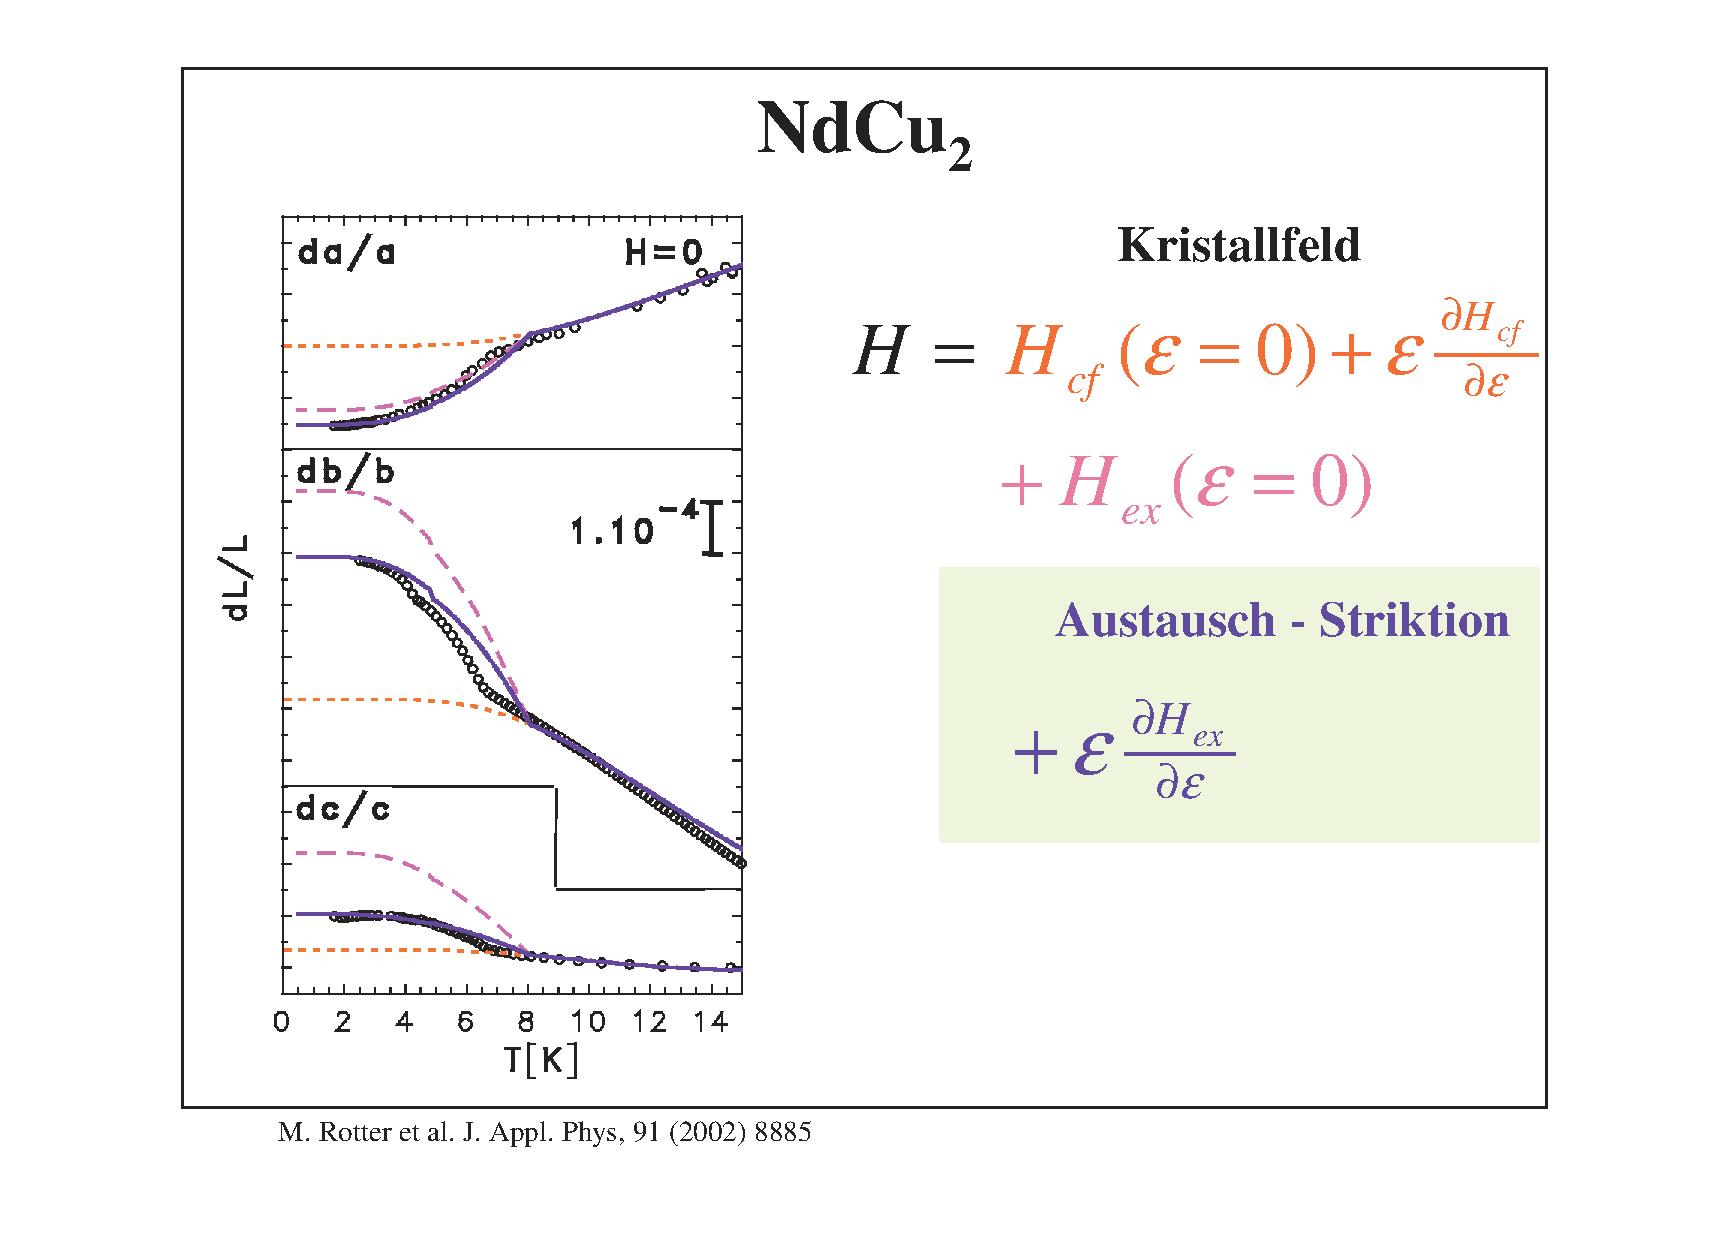
\includegraphics[angle=0, width=0.8\textwidth]{figsrc/magnetostriction_ndcu2.eps}
\end{center}
\caption{Calculated spontaneous magnetostriction of NdCu$_2$.}
\label{magnetostrictiongraphic}
\end{figure}

\begin{description}
\item [\prg mcphas.qvc]    the set of test q-vectors used for calculation of free energy.
                           Components of these q vectors refer to the reciprocal lattice $\vec a^*,\vec b^*,\vec c^*$.
\item [\prg mcphas.phs]    spin-configuration table of different types of spin-configurations. 
                            Note, in case of non-orthogonal axes the convention in these tables 
                            is $mb||\vec b$, $mc||(\vec a \times \vec b)$ and $ma$ perpendicular to $mb$ and $mc$.

                           {\em Note}: 
                           there is no natural criteria for deciding, if one spin-configuration is
			   different from another one. Therefore the list of ''different''
			   spin-configurations is dependent on the meaning of ''different''.
			   
			   The program {\prg McPhase} decides whether a spin-configuration is
			   different from another by a simple criteria, namely by the
			   angle between the spins. Comparing two spin configurations it calculates
			   the angle between corresponding spins and if for one spin the
			   angle is not small, the configuration is treated as a different
			   configuration. Therefore for example a ferromagnet with moments
			   in $a$ has a different spin configuration than a ferromagnet with
			   moments in $b$ direction. 
\item [\prg mcphas.sps]    $T-H$ dependence of spin-configuration. The spin configurations stored in this
                           file may be displayed using the program {\prg spins\index{spins}}, an example is given
			   in figure~\ref{spingraphic}.
                            Note, in case of non-orthogonal axes the convention for applied field $Ha, Hb,Hc$ and
                            also for the moment components $ma, mb, mc$ in these tables 
                            is $mb||\vec b$, $mc||(\vec a \times \vec b)$ and $ma$ perpendicular to $mb$ and $mc$.

\item [\prg mcphas.mf]     $T-H$ dependence of exchange field configuration, stored as $g_J \mu_B H_{xc}(i)$(unit is in meV)
                            for i=1,2,...,number of spins in magnetic unit cell.
                            Note, in case of non-orthogonal axes the convention for applied field $Ha, Hb,Hc$ and
                            also for the mean field components in these tables 
                            is $Hb||\vec b$, $Hc||(\vec a \times \vec b)$ and $Ha$ perpendicular to $Hb$ and $Hc$.
\item [\prg mcphas.fum]    free energy, magnetic energy (the derivative with respect to temperature gives the specific %%@
heat),
                           magnetisation data and (if cfield is used with higher order interactions)
                           expectation values of the Stevens Operators $<O_l^m>$ . As an example for the information
			   contained in this file the calculated magnetisation and magnetostriction of NdCu$_2$ is shown in
			   figures~\ref{magnetization} and ~\ref{magnetizationgraphic}.
                            Note, in case of non-orthogonal axes the convention for applied field $Ha, Hb,Hc$ and
                            also for the magnetisation components $ma,mb,mc$ in these tables 
                            is $Hb||\vec b$, $Hc||(\vec a \times \vec b)$ and $Ha$ perpendicular to $Hb$ and $Hc$.

\item [\prg mcphas1.j1 .j1 .j2 ...] 
               spin-spin correlation functions for sub-lattice 1 neighbour 1 2 ...
	       (linear combination is proportional to magnetostriction)
	       The spin-spin correlation functions for neighbour $k$ are defined by
	       the following sum of dyadic products:

	       \begin{equation}
	        \frac{1}{n}\sum_{s=1}^n <{\mbf J}^s> \times  <{\mbf J}^{s+k}>
	       \end{equation}
	       with $n$ being the number of moments in the magnetic unit cell.
	       Single ion and two-ion magnetostriction can be calculated using the $<O_l^m>$ and the
	       spin-spin correlation functions. As an example the magnetostriction analysis of
	       NdCu$_2$ is shown in figure~\ref{magnetostrictiongraphic}. For details 
             please refer to~\cite{rotter02-8885}.
                            Note, in case of non-orthogonal axes the convention for applied field $Ha, Hb,Hc$ and
                            also for the moment components in these tables 
                            is $Hb||\vec b$, $Hc||(\vec a \times \vec b)$ and $Ha$ perpendicular to $Hb$ and $Hc$.
\item [\prg mcphas.xyt]    phase diagram as x,y,T, H, phase-number j according to spin-configuration table
               given in mcphas.phs, a periodicity key, nettomoments <J>.
 Figure~\ref{phasediagramgraphic}
	       shows the phase diagram of NdCu$_2$ for magnetic fields parallel to the orthorhombic $b$-direction.
                            Note, in case of non-orthogonal axes the convention for applied field $Ha, Hb,Hc$ 
                             in these tables 
                            is $Hb||\vec b$, $Hc||(\vec a \times \vec b)$ and $Ha$ perpendicular to $Hb$ and $Hc$.
\item [\prg mcphas.hkl]    calculated (unpolarised) neutron diffraction data (the calculated magnetic intensities
    correspond to the magnetic structure + Polarisation factor. The
    Lorentz-factor , magnetic form factor and  instrumental corrections are not calculated.)
 As an example figure~\ref{neutintgraphic}
    shows the calculated temperature dependence of magnetic amplitudes for NdCu$_2$.
                           $h,k,l$ refer to the reciprocal lattice $\vec a^*,\vec b^*,\vec c^*$.
                            Note, in case of non-orthogonal axes the convention for applied field $Ha, Hb,Hc$ 
                             in these tables 
                            is $Hb||\vec b$, $Hc||(\vec a \times \vec b)$ and $Ha$ perpendicular to $Hb$ and $Hc$.
    
\item [\prg mcphasa.hkl]    Fourier Transform of the $a$-component of the magnetic Moments.
                           $h,k,l$ refer to the reciprocal lattice $\vec a^*,\vec b^*,\vec c^*$.
                            Note, in case of non-orthogonal axes the convention for applied field $Ha, Hb,Hc$ and
                            the magnetic moment component in these tables 
                            is $Hb||\vec b$, $Hc||(\vec a \times \vec b)$ and $Ha$ perpendicular to $Hb$ and $Hc$.
\item [\prg mcphasb.hkl]    Fourier Transform of the $b$-component of the magnetic Moments.
                           $h,k,l$ refer to the reciprocal lattice $\vec a^*,\vec b^*,\vec c^*$.
                            Note, in case of non-orthogonal axes the convention for applied field $Ha, Hb,Hc$ and
                            the magnetic moment component in these tables 
                            is $Hb||\vec b$, $Hc||(\vec a \times \vec b)$ and $Ha$ perpendicular to $Hb$ and $Hc$.
\item [\prg mcphasc.hkl]    Fourier Transform of the $c$-component of the magnetic Moments.
                           $h,k,l$ refer to the reciprocal lattice $\vec a^*,\vec b^*,\vec c^*$.
                            Note, in case of non-orthogonal axes the convention for applied field $Ha, Hb,Hc$ and
                            the magnetic moment component in these tables 
                            is $Hb||\vec b$, $Hc||(\vec a \times \vec b)$ and $Ha$ perpendicular to $Hb$ and $Hc$.
\end{description} 

\vspace{1cm}
{\em Exercises:}
\begin{itemize}
\item Look at the output files of {\prg McPhase}  in the directory
{\prg examples/ndcu2b\_new/results}.  At which magnetic field
the ferromagnetically aligned state is achieved (at $T=$2~K)?
\item
What is the propagation vector in the different antiferromagnetic phases at $T=$2~K ?
\end{itemize}





\subsubsection{{\prg mcphas.j\index{mcphas.j}} - lattice and exchange parameters}\label{mcphasj}
This file provides the information about 
the crystallographic
 structure and the magnetic exchange interactions.
For every atom in the crystallographic basis there
has to be given the coordinates, the number of neighbours to be considered, the 
Land\'e factor $g_J$, the single ion property filename and  a set of exchange parameters.
If the exchange parameters (and neighbour positions) are not known for your system, you 
can use the program module {\prg makenn\index{makenn}} (see section \ref{addprog}) to generate 
a list of nearest neighbours and
exchange parameters, currently implemented in {\prg makenn\index{makenn}} are dipolar interactions,
exchange interactions via the Bethe-Slater curve or the RKKY model. Note that in order
to use {\prg makenn\index{makenn}} you have to set up a working {\prg mcphas.j\index{mcphas.j}} file, which may or
may not contain neighbours and interactions.

Use program {\prg addj\index{addj}} to add exchange parameter set stored in different 
such {\prg .j} files (see section~\ref{addprog}).



\begin{description}
\item [Line 1,2:] Comment Lines
\item [Line 3:] lattice constants a,b,c and crystal angles alpha, beta, gamma 
\item [Line 4-6:] primitive lattice vectors
\item [Line 7:] Number of atoms in the primitive crystallographic unit cell ({\prg nofatoms})
\item [Line 8:] a comment line with stars
\item [Line 9:] coordinates  ($d_a$,$d_b$,$d_c$) of 1$^{st}$ magnetic ion in the crystallographic unit cell  with
respect to the lattice vectors $\vec a$,$\vec b$,$\vec c$. The number of neighbours of this 
ion, for which interaction constants are given in the interaction table (nofneighbours). 
If {\prg diagonalexchange}
is set to 0 the 9 components of the exchange tensor are given in column 4-12. 
If {\prg diagonalexchange}
 is 1, only 3 components are given (column 4-6).
If {\prg diagonalexchange}
 is 2, specific components of the exchange tensor can be given in columns 4 onwards. The indices of these components
 must be given in the following line (Line 9a below).
The Land\'e factor of the ion (gJ) and the file name of the corresponding single ion
parameter file (cffilename).
\item [Line 9a:]  If {\prg diagonalexchange=2}, then this line gives the indices of the exchange tensor corresponding to 
 the columns 4 onwards. It must have a variable called {\prg indexexchange} followed by a list of names of components of the interaction
 tensor separated by space. E.g.
 \verb|  #! indexexchange= JaJb JbJc  | 
means column 4 gives the the interaction constant between the
 first angular momentum component of the current ion with the second angular momentum component of its neighbour, whilst 
 column 5 has the interaction constant between the second angular momentum component of this ion with the third component of its
 neighbour. Alternatively, pairs of numbers may be given, as in \verb|  #! indexexchange= 1,2 2,3  |
 Additionally another parameter {\prg symmetricexchange} can be set to 1, where the value in each column is also used 
 for the transposed tensor component. Thus \verb|  #! symmetricexchange=1 indexexchange= JaJb  | is the same as \\
 \verb|  #! indexexchange= JaJb JbJa  | where the 4th and 5th column are the same.
\item [Line 10:]  Comment line
\item [Line 11-(10+nofneighbours):] Interaction table for ion number 1.   
Note: the neighbour coordinates (column 1-3) are given with respect to the lattice vectors
$\vec a$,$\vec b$,$\vec c$. The program then calculates from these values the coordinates
with respect to the primitive lattice $\vec r_1$,~$\vec r_2$,~$\vec r_3$.
($ d_a \vec a + d_b \vec b + d_c \vec c = d_1 \vec r_1 + d_2 \vec r_2 + d_3 \vec r_3$).
Column 4,5,6 \dots contain the components of the interaction tensor $\stackrel{=}{\mathcal J}$. 
Note that in case of non-orthogonal axes the 
components of the moments and the interaction tensor $Ja, Jb, Jc, Jaa, Jbb, Jcc, Jab ...$ 
refer to the orthogonal coordinate system
defined with respect to the nonorthogonal lattice $\vec a,\vec b,\vec c$ as
$Jb||\vec b$, $Jc||(\vec a \times \vec b)$ and $Ja$ perpendicular to $Jb$ and $Jc$.
\item [Line (11+nofneighbours) - end:] for each ion in the unit cell line 8 - (10+nofneighbours)
are repeated.
\end{description}


\vspace{0.5cm}

{\small {\bf Information for experienced users:}
\begin{description}
\item[\prg mcphas.jjj:]
format of exchange parameter file, which only needs a reduced set of exchange
parameters in the input file. Using the program {\prg jjj2j} the file can be transformed
to {\prg mcphas.j\index{mcphas.j}} by adding lines for all the equivalent neighbours. The format definition
of {\prg mcphas.jjj} is the same as {\prg mcphas.j\index{mcphas.j}}, however each line denotes several
equivalent neighbour atoms (instead of only one in {\prg mcphas.j\index{mcphas.j}}) according to the
 following rules:
\begin{itemize}
\item If a nonzero coordinate $d_a$ (or $d_b$,$d_c$) in the interaction table
 corresponds to it's value at the nearest
 lattice point of the primitive lattice,
  additional interactions of the same size
with  neighbours with coordinate $-d_a$ (or $-d_b$,$-d_c$, respectively)
are taken into account. This
holds for each of the three coordinates $d_a$,$d_b$ and $d_c$
 resulting in a maximum
number of 8 equivalent neighbours per line in the interaction table.
\item If the value of $d_a$ (or $d_b$,$d_c$) is zero or differs
from it's value at the nearest lattice point of the primitive lattice, it is 
changed to the value at the nearest lattice point and {\bf no} interaction 
with  neighbours with coordinates $-d_a$ (or $-d_b$,$-d_c$) is
 taken into account. If such
 interaction is needed it may be given in a different line and may
have different magnitude. In this way also crystallographic lattices
with no mirror symmetry may be described.
\end{itemize}
\item[\prg mcphas.coq:]   exchange parameters etc [ in old format]...see examples for details, use {\prg coq2jjj} to 
transform {\prg mcphas.coq} to {\prg mcphas.jjj} format
\end{description}

}


\subsubsection{Example {\prg mcphas.j\index{mcphas.j}} file for a simple antiferromagnet}

Here are example files of a tetragonal antiferromagnet with nearest neighbour interactions, all
files are equivalent:

{\small
\begin{verbatim} 
# simple antiferromagnet 
#<!--mcphase.mcphas.j-->
#***************************************************************
# Lattice Constants (A)
#! a=4.3843 b=4.3843 c=2.4194 alpha=  90 beta=  90 gamma=  90
#! r1a=   1 r2a=   0 r3a=   0
#! r1b=   0 r2b=   1 r3b=   0   primitive lattice vectors [a][b][c]
#! r1c=   0 r2c=   0 r3c=   1
#! nofatoms=1  nofcomponents=3  number of atoms in primitive unit cell/number of components of each spin
# ****************************************************************************
#! da=  0 [a] db=  0 [b] dc=  0 nofneighbours=2 diagonalexchange=0 gJ=0.857143 cffilename=Ce3p.sipf
# da[a] db[b] dc[c] Jaa[meV] Jbb[meV] Jcc[meV] Jab[meV] Jba[meV] Jac[meV] Jca[meV] Jbc[meV] Jcb[meV]
+0	+0	+1	-0.1	-0.1	-0.1   0  0  0  0  0  0
+0	+0	-1	-0.1	-0.1	-0.1   0  0  0  0  0  0
#\end{verbatim}
}

Using diagonalexchange this may be shortened to

{\small
\begin{verbatim} 
# simple antiferromagnet 
#<!--mcphase.mcphas.j-->
#***************************************************************
# Lattice Constants (A)
#! a=4.3843 b=4.3843 c=2.4194 alpha=  90 beta=  90 gamma=  90
#! r1a=   1 r2a=   0 r3a=   0
#! r1b=   0 r2b=   1 r3b=   0   primitive lattice vectors [a][b][c]
#! r1c=   0 r2c=   0 r3c=   1
#! nofatoms=1  nofcomponents=3  number of atoms in primitive unit cell/number of components of each spin
# ****************************************************************************
#! da=  0 [a] db=  0 [b] dc=  0 nofneighbours=2 diagonalexchange=1 gJ=0.857143 cffilename=Ce3p.sipf
# da[a] db[b] dc[c] Jaa[meV] Jbb[meV] Jcc[meV] Jab[meV] Jba[meV] Jac[meV] Jca[meV] Jbc[meV] Jcb[meV]
+0	+0	+1	-0.1	-0.1	-0.1   
+0	+0	-1	-0.1	-0.1	-0.1   
#\end{verbatim}
}

with indexexchange option the sequence of two ion interaction parameters can be changed and
zero parameters may be omitted:

{\small
\begin{verbatim} 
# simple antiferromagnet 
#<!--mcphase.mcphas.j-->
#***************************************************************
# Lattice Constants (A)
#! a=4.3843 b=4.3843 c=2.4194 alpha=  90 beta=  90 gamma=  90
#! r1a=   1 r2a=   0 r3a=   0
#! r1b=   0 r2b=   1 r3b=   0   primitive lattice vectors [a][b][c]
#! r1c=   0 r2c=   0 r3c=   1
#! nofatoms=1  nofcomponents=3  number of atoms in primitive unit cell/number of components of each spin
# ****************************************************************************
#! da=  0 [a] db=  0 [b] dc=  0 nofneighbours=2 diagonalexchange=2 gJ=0.857143 cffilename=Ce3p.sipf
# da[a] db[b] dc[c] Jaa[meV] Jbb[meV] Jcc[meV] Jab[meV] Jba[meV] Jac[meV] Jca[meV] Jbc[meV] Jcb[meV]
#! indexexchange = JaJa JaJc JcJa JbJb JcJc
+0	+0	+1	-0.1 0 0 -0.1	-0.1  
+0	+0	-1	-0.1 0 0 -0.1	-0.1  
#\end{verbatim}
}

{\small
\begin{verbatim} 
# simple antiferromagnet 
#<!--mcphase.mcphas.j-->
#***************************************************************
# Lattice Constants (A)
#! a=4.3843 b=4.3843 c=2.4194 alpha=  90 beta=  90 gamma=  90
#! r1a=   1 r2a=   0 r3a=   0
#! r1b=   0 r2b=   1 r3b=   0   primitive lattice vectors [a][b][c]
#! r1c=   0 r2c=   0 r3c=   1
#! nofatoms=1  nofcomponents=3  number of atoms in primitive unit cell/number of components of each spin
# ****************************************************************************
#! da=  0 [a] db=  0 [b] dc=  0 nofneighbours=2 diagonalexchange=2 gJ=0.857143 cffilename=Ce3p.sipf
# da[a] db[b] dc[c] Jaa[meV] Jbb[meV] Jcc[meV] Jab[meV] Jba[meV] Jac[meV] Jca[meV] Jbc[meV] Jcb[meV]
#! indexexchange = 1,1 1,3, 3,1 2,2 3,3
+0	+0	+1	-0.1 0 0 -0.1	-0.1  
+0	+0	-1	-0.1 0 0 -0.1	-0.1  
#\end{verbatim}
}


using symmetricexchange together with indexexchange will assume that the interaction tensor is symmetic and 
only half of it may be given:

{\small
\begin{verbatim} 
# simple antiferromagnet 
#<!--mcphase.mcphas.j-->
#***************************************************************
# Lattice Constants (A)
#! a=4.3843 b=4.3843 c=2.4194 alpha=  90 beta=  90 gamma=  90
#! r1a=   1 r2a=   0 r3a=   0
#! r1b=   0 r2b=   1 r3b=   0   primitive lattice vectors [a][b][c]
#! r1c=   0 r2c=   0 r3c=   1
#! nofatoms=1  nofcomponents=3  number of atoms in primitive unit cell/number of components of each spin
# ****************************************************************************
#! da=  0 [a] db=  0 [b] dc=  0 nofneighbours=2 diagonalexchange=2 gJ=0.857143 cffilename=Ce3p.sipf
# da[a] db[b] dc[c] Jaa[meV] Jbb[meV] Jcc[meV] Jab[meV] Jba[meV] Jac[meV] Jca[meV] Jbc[meV] Jcb[meV]
#! symmetricexchange=1 indexexchange = JaJa JaJc JbJb JcJc
+0	+0	+1	-0.1 0  -0.1	-0.1  
+0	+0	-1	-0.1 0  -0.1	-0.1  
#\end{verbatim}
}


\subsubsection{Single Ion Property Input Files}\label{sifile}

In order to speed up calculations or treat special problems a large 
variety of single ion modules is available. This includes the
option to load a user written single ion module. Details are 
given in chapter~\ref{simod}.

The first time user of {\prg McPhase} should use the module {\prg so1ion}\index{so1ion} and 
create an appropriate single ion property input file as described in
section \ref{cf1ion}. A good starting point are several examples
given in directory {\prg examples}.


\subsubsection{Example single ion property file  for a simple antiferromagnet}

Here is an example file {\prg mcphas.cf1} describing the anisotropy of a 
simple antiferromagnet with Ce atoms having basal plane anisotropy. Note the
axis convention xyz$||$abc, in case of non-orthogonal axes the convention 
is $y||\vec b$, $z||(\vec a \times \vec b)$ and $x$ perpendicular to $y$ and $z$.


\section{{\prg mcphas} - calculation of thermodynamic properties (Magnetisation, Susceptibility, Specific Heat, Neutron %%@
Diffraction, etc.)}
\label{runmcphas}

In order to perform calculations beyond the capabilities of {\prg cfield\index{cfield}} it is necessary
to use the program {\prg mcphas}. 
\begin{itemize}
\item As a first step it is possible to
calculate the thermodynamic properties such as magnetisation or specific heat
considering only single ion effects. In this case all the exchange parameters
have to be set to zero in {\prg mcphas.j\index{mcphas.j}}. 
\item for more advanced calculations the two - ion interactions have to be
considered and may lead to magnetic order. {\prg mcphas} can perform 
calculations in the ordered state in the following way: for 
a given temperature $T$ and magnetic field $\mbf H$ (vector)
several possible magnetic structures are stabilised
by a mean field algorithm and the free energy is 
calculated. The initial values for this mean-field procedure are
modified by a Monte Carlo process.


The temperature and magnetic field is varied during the calculation
and thereby it is possible to map out the magnetic phase diagram.
\end{itemize}

The program produces a plot of the stabilised magnetic
structures and the magnetisation on screen, the
output files contain additional information 
such as calculated magnetoelastic and  neutron-scattering
data. Several graphic programs easy the visualisation of the
calculated data (section~\ref{graphics}).



\subsection{Input Files}
The program {\prg McPhase} needs the following input files (all in the same directory)
 in order to run:

\begin{enumerate}
\item {\prg mcphas.ini\index{mcphas.ini}}
 - controlling the algorithm
\item {\prg mcphas.j\index{mcphas.j}}
  - lattice and exchange parameters
\item {\prg mcphas.tst\index{mcphas.tst}(optional)}  - test spin configurations
\item {\prg single-ion property files}
\item {\prg directory ./results/}
 - directory where calculated data is stored
\item {\prg directory ./fit} - experimental data for fit (optional)
\end{enumerate}


 All
 of these input files have to be in one directory and the program
has to be started in this directory. The results of the simulation
are then stored in the  subdirectory ./results/, which must exist before starting
the program 
... see directory ./examples/ for some examples.
 In order to prepare these files
for a new calculation it is best to take them from an example, copy the files
to a new directory and make the
modifications  to adapt them to the new problem.

\subsubsection{Example - a simple antiferromagnet}

In the following description of the input files we will always refer
to a simple example: a simple antiferromagnet
on a primitive orthorhombic lattice. The first time user
will thus have a simple example to follow, all corresponding
files are given in the directory {\prg tutorial/03magnetic\_phases\_mcphas/simpleAF}.
 

\subsubsection{{\prg mcphas.ini\index{mcphas.ini}} - controlling the algorithm}
   Initial file containing algorithm control parameters, for instance the range and spacing of
   propagation vectors Q or the number of Monte Carlo trials for initial spin configurations
    - {\em mind}: this
   file is rewritten and reread  when running the program and may be changed by the
   user in order to manipulate the running simulation.

{\prg mcphas.ini\index{mcphas.ini}} consists of several sections:
\begin{description}
\item [MCPHASE RUNTIME CONTROL:] this section contains the parameters
controlling the status of the calculation.
\item [XY PHASEDIAGRAM PARAMETERS:] here the temperature and field range and
step widths of the calculation are specified.
The definition of the x and y
axis in terms of temperature and magnetic field is followed by the
corresponding range and step width. An offset may be given for all
field and temperature values.
Note that for most cases of interest
this offset is zero (T0=0, Ha0=0, Hb0=0, Hc0=0).
 For the simple case of calculating a Temperature-Field phase diagram
 It is just necessary to set xT=1 and give the temperature range by
xmin/xmax/xstep. For field in b direction then just set yHb=1 and 
define the range in ymin/ymax/ystep.
In case of non-orthogonal axes the applied magnetic field
components $Ha, Hb, Hc$ refer to the orthogonal coordinate system
defined with respect to the nonorthogonal lattice $\mbf a,\mbf b,\mbf c$ as
$Hb||\mbf b$, $Hc||(\mbf a \times \mbf b)$ and $Ha$ perpendicular to $Hb$ and $Hc$.

\item [GENERATION OF SPINCONFIGURATIONS:] at the beginning of the program
some initial values of spin configurations are generated from a set of 
propagation vectors. This section defines the range of propagation vectors
and the step width.
Depending on the value of the propagation Q with respect to the primitive reciprocal lattice
1-, 2- or 3-dimensional simulations of magnetic lattices
are possible. It is advisable to 
think carefully about the chosen range and spacing of Q vectors in order
to limit calculation time.
 
For example a good starting point is to begin with a calculation with large
step widths (e.g. 0.1)  covering the Brillouin zone. This should give an idea
of the propagation vectors which are stabilised. An advanced calculation
could then fine tune the propagation and determine its accurate value (using
small step widths in a limited area of the zone).
The verbose option of {\prg mcphas} allows to inspect the propagation vectors
which are actually used in the calculation.
Trick: in order to get a quick overview of the
q-vector range covered by the mcphas\index{mcphas} simulation start mcphas, exit and 
just type {\prg felog ./results/mcphas.qvc} (need {\prg perl,perldl,pdl,pgplot} packages).

In order to limit calculation time, the maximum periodicity
of the magnetic unit cell with respect to the crystallographic unit cell 
(maxqperiod) and the maximum number of spins in the magnetic unit cell 
(maxnofspins) can be limited. Also the maximum number of test spin configurations
in the internal table can be limited (maxnoftestspincf).
A critical feature with respect to calculation time is also the number of
spin configurations which are generated by a random process from a tabulated
SPINCONFIGURATIONS during the calculation. 

In summary the variables in this section are mainly important to adapt the
program to a given computer system with finite speed. They have to be set
to optimise between speed and accuracy of the calculation. In order to
find appropriate values it is best to perform some calculations 
and restrict the parameters step by step if insufficient speed is obtained.
Also the examples included in the program package may serve as starting
points.

\item [PARAMETERS FOR SUB FECALC SELFCONSISTENCY PROCESS:] the most important
procedure in the module {\prg mcphas} is the sub fecalc. In this part of the 
program the self consistent calculation of the magnetic moment configuration
is performed as shown schematically in fig.~\ref{fecalc}. 
In the mean field approximation the Hamiltonian~(\ref{hamilton}) is approximated
by

\begin{equation}
 {\mathcal H}=\sum_n H_{SI}^n + E_{corr}
\end{equation}

with the single ion Hamiltonian (in case of module {\prg so1ion\index{so1ion}})

\begin{equation}
H_{SI}^n=  B_l^m O_{lm}({\mbf J}^n) 
	     - g_{Jn} \mu_B {\mbf J}^n {\mbf H^n_{eff}} 
\end{equation}

and the correction term

\begin{equation}
E_{corr}=\frac{1}{2}\sum_{n} g_{Jn} \mu_B \langle {\mbf J}^n
 \rangle (\mbf H^n_{eff}-\mbf H) 
\end{equation}

and with the mean fields $ \mbf H^n_{eff}$ given by

\begin{equation}\label{meanfield}
\mbf H^n_{eff}=\mbf H + \mbf H^n_{xc}=\mbf H+\sum_{{\mbf G'}n'} \frac{{\mathcal J}
(\mbf r_n-(\mbf G'+\mbf r_{n'}))}{g_{Jn}\mu_B } \langle{\mbf
J}^{n'}\rangle
\end{equation}

These mean fields and the moments $\langle \mbf J^n \rangle$ 
are determined in a self consistent
way. For a given magnetic unit cell and initial configuration 
of magnetic moments
the mean fields are calculated according to equation~(\ref{meanfield}). 
Then, for each
magnetic ion the single ion property module is taken 
and the magnetic moment $\langle \mbf J^n \rangle$ is 
calculated from it's mean field. The mean fields are used again in equation~(\ref{meanfield})
and so on .... until convergence is reached. 
Then, the free energy ($f=-kT\sum_n \ln(z_n) + E_{corr}$ ) 
of the stabilised
configuration is calculated (this is why this sub is called {\prg fecalc}). 
The free energies of a lot of different stabilised configurations have to
be compared in order to find out which configuration has lowest free energy, i.e.
is stable in thermal  equilibrium.

It may happen that this process does
not converge due to bad choice of the initial configuration, therefore a maximum number
of mean field loops has to be given by the user.
The results of a calculation may be significantly influenced by
changing parameters such as the maximum number of iteration loops 
in this section. 
In fact the simulation is always a compromise of calculation time and accuracy: if only
a few initial spin configurations are tried at each (H-T) point, the calculation speed is
fast, however it is possible that the program misses the magnetic structure with the
lowest free energy. The same holds if other critical parameters of the simulation are
restricted too much.
 

\item [OUTPUT OF PHYSICAL PROPERTIES:]
Some options for the output of the calculation can be changed in this section.
\end{description}

\begin{figure}[hb]
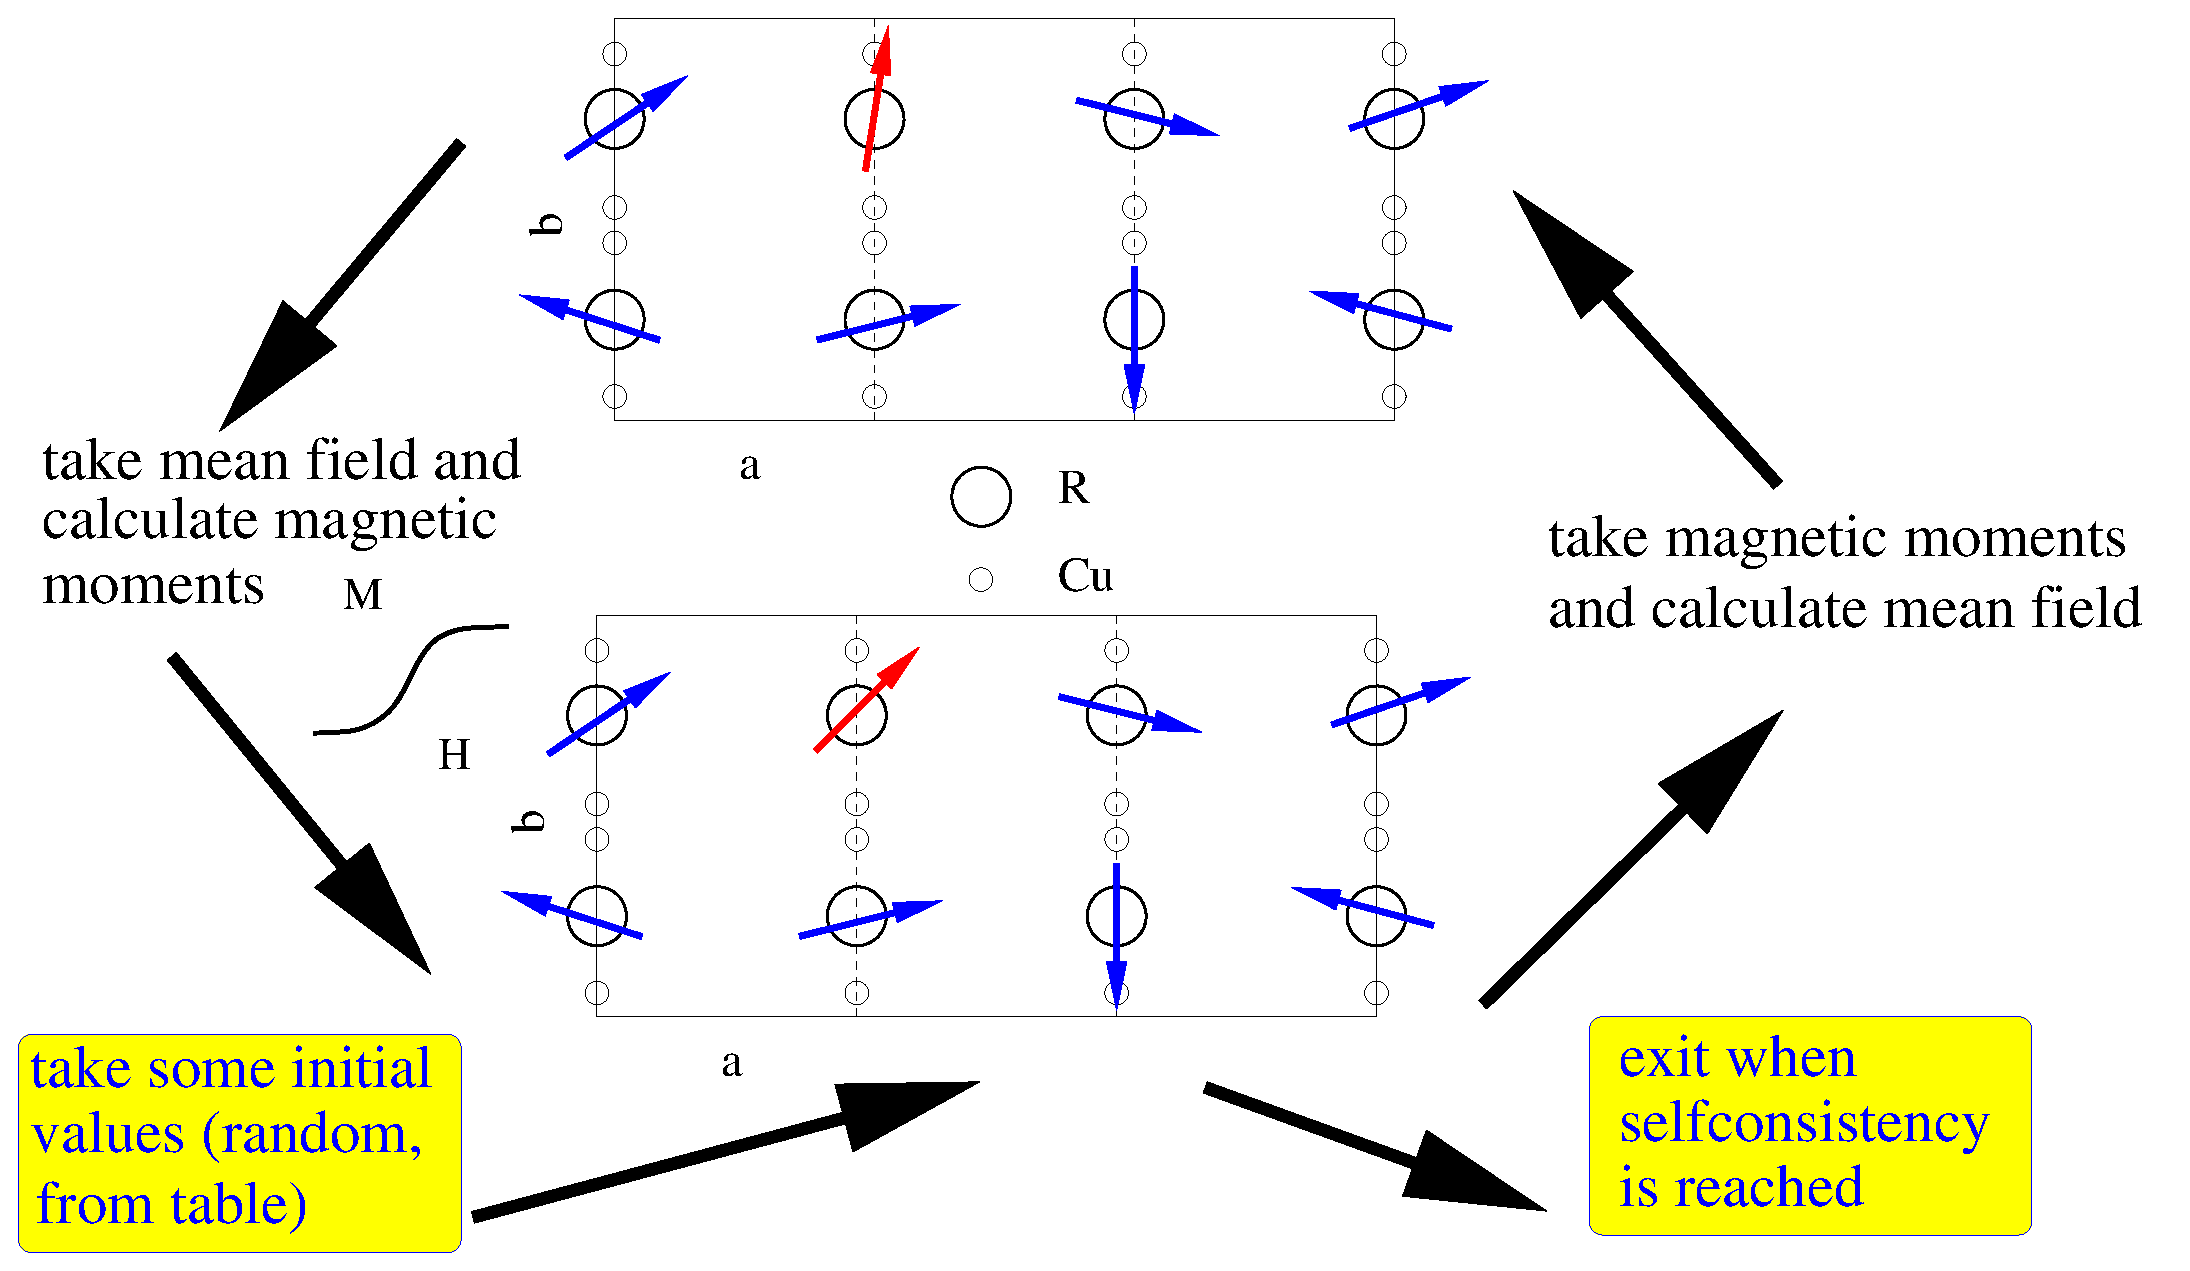
\includegraphics[angle=0,width=0.9\columnwidth]{figsrc/fecalc.eps}
\caption{\label{fecalc}Mean field process of sub {\prg fecalc}.}
\end{figure}

 
\subsubsection{Example {\prg mcphas.ini\index{mcphas.ini}} file for a simple antiferromagnet}

Here is an example of {\prg mcphas.ini\index{mcphas.ini}}, the comments describe the meaning of the different
parameters:

\input{mcphas.ini}



\subsubsection{{\prg mcphas.j\index{mcphas.j}} - lattice and exchange parameters}\label{mcphasj}
This file provides the information about 
the crystallographic
 structure and the magnetic exchange interactions.
For every atom in the crystallographic basis there
has to be given the coordinates, the number of neighbours to be considered, the 
Land\'e factor $g_J$, the single ion property filename and  a set of exchange parameters.
If the exchange parameters (and neighbour positions) are not known for your system, you 
can use the program module {\prg makenn\index{makenn}} (see section \ref{addprog}) to generate 
a list of nearest neighbours and
exchange parameters, currently implemented in {\prg makenn\index{makenn}} are dipolar interactions,
exchange interactions via the Bethe-Slater curve or the RKKY model. Note that in order
to use {\prg makenn\index{makenn}} you have to set up a working {\prg mcphas.j\index{mcphas.j}} file, which may or
may not contain neighbours and interactions.

Use program {\prg addj\index{addj}} to add exchange parameter set stored in different 
such {\prg .j} files (see section~\ref{addprog}).



\begin{description}
\item [Line 1,2:] Comment Lines
\item [Line 3:] lattice constants a,b,c and crystal angles alpha, beta, gamma 
\item [Line 4-6:] primitive lattice vectors
\item [Line 7:] Number of atoms in the primitive crystallographic unit cell ({\prg nofatoms})
\item [Line 8:] a comment line with stars
\item [Line 9:] coordinates  ($d_a$,$d_b$,$d_c$) of 1$^{st}$ magnetic ion in the crystallographic unit cell  with
respect to the lattice vectors $\vec a$,$\vec b$,$\vec c$. The number of neighbours of this 
ion, for which interaction constants are given in the interaction table (nofneighbours). 
If {\prg diagonalexchange}
is set to 0 the 9 components of the exchange tensor are given in column 4-12. 
If {\prg diagonalexchange}
 is 1, only 3 components are given (column 4-6).
If {\prg diagonalexchange}
 is 2, specific components of the exchange tensor can be given in columns 4 onwards. The indices of these components
 must be given in the following line (Line 9a below).
The Land\'e factor of the ion (gJ) and the file name of the corresponding single ion
parameter file (cffilename).
\item [Line 9a:]  If {\prg diagonalexchange=2}, then this line gives the indices of the exchange tensor corresponding to 
 the columns 4 onwards. It must have a variable called {\prg indexexchange} followed by a list of names of components of the interaction
 tensor separated by space. E.g.
 \verb|  #! indexexchange= JaJb JbJc  | 
means column 4 gives the the interaction constant between the
 first angular momentum component of the current ion with the second angular momentum component of its neighbour, whilst 
 column 5 has the interaction constant between the second angular momentum component of this ion with the third component of its
 neighbour. Alternatively, pairs of numbers may be given, as in \verb|  #! indexexchange= 1,2 2,3  |
 Additionally another parameter {\prg symmetricexchange} can be set to 1, where the value in each column is also used 
 for the transposed tensor component. Thus \verb|  #! symmetricexchange=1 indexexchange= JaJb  | is the same as \\
 \verb|  #! indexexchange= JaJb JbJa  | where the 4th and 5th column are the same.
\item [Line 10:]  Comment line
\item [Line 11-(10+nofneighbours):] Interaction table for ion number 1.   
Note: the neighbour coordinates (column 1-3) are given with respect to the lattice vectors
$\vec a$,$\vec b$,$\vec c$. The program then calculates from these values the coordinates
with respect to the primitive lattice $\vec r_1$,~$\vec r_2$,~$\vec r_3$.
($ d_a \vec a + d_b \vec b + d_c \vec c = d_1 \vec r_1 + d_2 \vec r_2 + d_3 \vec r_3$).
Column 4,5,6 \dots contain the components of the interaction tensor $\stackrel{=}{\mathcal J}$. 
Note that in case of non-orthogonal axes the 
components of the moments and the interaction tensor $Ja, Jb, Jc, Jaa, Jbb, Jcc, Jab ...$ 
refer to the orthogonal coordinate system
defined with respect to the nonorthogonal lattice $\vec a,\vec b,\vec c$ as
$Jb||\vec b$, $Jc||(\vec a \times \vec b)$ and $Ja$ perpendicular to $Jb$ and $Jc$.
\item [Line (11+nofneighbours) - end:] for each ion in the unit cell line 8 - (10+nofneighbours)
are repeated.
\end{description}


\vspace{0.5cm}

{\small {\bf Information for experienced users:}
\begin{description}
\item[\prg mcphas.jjj:]
format of exchange parameter file, which only needs a reduced set of exchange
parameters in the input file. Using the program {\prg jjj2j} the file can be transformed
to {\prg mcphas.j\index{mcphas.j}} by adding lines for all the equivalent neighbours. The format definition
of {\prg mcphas.jjj} is the same as {\prg mcphas.j\index{mcphas.j}}, however each line denotes several
equivalent neighbour atoms (instead of only one in {\prg mcphas.j\index{mcphas.j}}) according to the
 following rules:
\begin{itemize}
\item If a nonzero coordinate $d_a$ (or $d_b$,$d_c$) in the interaction table
 corresponds to it's value at the nearest
 lattice point of the primitive lattice,
  additional interactions of the same size
with  neighbours with coordinate $-d_a$ (or $-d_b$,$-d_c$, respectively)
are taken into account. This
holds for each of the three coordinates $d_a$,$d_b$ and $d_c$
 resulting in a maximum
number of 8 equivalent neighbours per line in the interaction table.
\item If the value of $d_a$ (or $d_b$,$d_c$) is zero or differs
from it's value at the nearest lattice point of the primitive lattice, it is 
changed to the value at the nearest lattice point and {\bf no} interaction 
with  neighbours with coordinates $-d_a$ (or $-d_b$,$-d_c$) is
 taken into account. If such
 interaction is needed it may be given in a different line and may
have different magnitude. In this way also crystallographic lattices
with no mirror symmetry may be described.
\end{itemize}
\item[\prg mcphas.coq:]   exchange parameters etc [ in old format]...see examples for details, use {\prg coq2jjj} to 
transform {\prg mcphas.coq} to {\prg mcphas.jjj} format
\end{description}

}


\subsubsection{Example {\prg mcphas.j\index{mcphas.j}} file for a simple antiferromagnet}

Here are example files of a tetragonal antiferromagnet with nearest neighbour interactions, all
files are equivalent:

{\small
\begin{verbatim} 
# simple antiferromagnet 
#<!--mcphase.mcphas.j-->
#***************************************************************
# Lattice Constants (A)
#! a=4.3843 b=4.3843 c=2.4194 alpha=  90 beta=  90 gamma=  90
#! r1a=   1 r2a=   0 r3a=   0
#! r1b=   0 r2b=   1 r3b=   0   primitive lattice vectors [a][b][c]
#! r1c=   0 r2c=   0 r3c=   1
#! nofatoms=1  nofcomponents=3  number of atoms in primitive unit cell/number of components of each spin
# ****************************************************************************
#! da=  0 [a] db=  0 [b] dc=  0 nofneighbours=2 diagonalexchange=0 gJ=0.857143 cffilename=Ce3p.sipf
# da[a] db[b] dc[c] Jaa[meV] Jbb[meV] Jcc[meV] Jab[meV] Jba[meV] Jac[meV] Jca[meV] Jbc[meV] Jcb[meV]
+0	+0	+1	-0.1	-0.1	-0.1   0  0  0  0  0  0
+0	+0	-1	-0.1	-0.1	-0.1   0  0  0  0  0  0
#\end{verbatim}
}

Using diagonalexchange this may be shortened to

{\small
\begin{verbatim} 
# simple antiferromagnet 
#<!--mcphase.mcphas.j-->
#***************************************************************
# Lattice Constants (A)
#! a=4.3843 b=4.3843 c=2.4194 alpha=  90 beta=  90 gamma=  90
#! r1a=   1 r2a=   0 r3a=   0
#! r1b=   0 r2b=   1 r3b=   0   primitive lattice vectors [a][b][c]
#! r1c=   0 r2c=   0 r3c=   1
#! nofatoms=1  nofcomponents=3  number of atoms in primitive unit cell/number of components of each spin
# ****************************************************************************
#! da=  0 [a] db=  0 [b] dc=  0 nofneighbours=2 diagonalexchange=1 gJ=0.857143 cffilename=Ce3p.sipf
# da[a] db[b] dc[c] Jaa[meV] Jbb[meV] Jcc[meV] Jab[meV] Jba[meV] Jac[meV] Jca[meV] Jbc[meV] Jcb[meV]
+0	+0	+1	-0.1	-0.1	-0.1   
+0	+0	-1	-0.1	-0.1	-0.1   
#\end{verbatim}
}

with indexexchange option the sequence of two ion interaction parameters can be changed and
zero parameters may be omitted:

{\small
\begin{verbatim} 
# simple antiferromagnet 
#<!--mcphase.mcphas.j-->
#***************************************************************
# Lattice Constants (A)
#! a=4.3843 b=4.3843 c=2.4194 alpha=  90 beta=  90 gamma=  90
#! r1a=   1 r2a=   0 r3a=   0
#! r1b=   0 r2b=   1 r3b=   0   primitive lattice vectors [a][b][c]
#! r1c=   0 r2c=   0 r3c=   1
#! nofatoms=1  nofcomponents=3  number of atoms in primitive unit cell/number of components of each spin
# ****************************************************************************
#! da=  0 [a] db=  0 [b] dc=  0 nofneighbours=2 diagonalexchange=2 gJ=0.857143 cffilename=Ce3p.sipf
# da[a] db[b] dc[c] Jaa[meV] Jbb[meV] Jcc[meV] Jab[meV] Jba[meV] Jac[meV] Jca[meV] Jbc[meV] Jcb[meV]
#! indexexchange = JaJa JaJc JcJa JbJb JcJc
+0	+0	+1	-0.1 0 0 -0.1	-0.1  
+0	+0	-1	-0.1 0 0 -0.1	-0.1  
#\end{verbatim}
}

{\small
\begin{verbatim} 
# simple antiferromagnet 
#<!--mcphase.mcphas.j-->
#***************************************************************
# Lattice Constants (A)
#! a=4.3843 b=4.3843 c=2.4194 alpha=  90 beta=  90 gamma=  90
#! r1a=   1 r2a=   0 r3a=   0
#! r1b=   0 r2b=   1 r3b=   0   primitive lattice vectors [a][b][c]
#! r1c=   0 r2c=   0 r3c=   1
#! nofatoms=1  nofcomponents=3  number of atoms in primitive unit cell/number of components of each spin
# ****************************************************************************
#! da=  0 [a] db=  0 [b] dc=  0 nofneighbours=2 diagonalexchange=2 gJ=0.857143 cffilename=Ce3p.sipf
# da[a] db[b] dc[c] Jaa[meV] Jbb[meV] Jcc[meV] Jab[meV] Jba[meV] Jac[meV] Jca[meV] Jbc[meV] Jcb[meV]
#! indexexchange = 1,1 1,3, 3,1 2,2 3,3
+0	+0	+1	-0.1 0 0 -0.1	-0.1  
+0	+0	-1	-0.1 0 0 -0.1	-0.1  
#\end{verbatim}
}


using symmetricexchange together with indexexchange will assume that the interaction tensor is symmetic and 
only half of it may be given:

{\small
\begin{verbatim} 
# simple antiferromagnet 
#<!--mcphase.mcphas.j-->
#***************************************************************
# Lattice Constants (A)
#! a=4.3843 b=4.3843 c=2.4194 alpha=  90 beta=  90 gamma=  90
#! r1a=   1 r2a=   0 r3a=   0
#! r1b=   0 r2b=   1 r3b=   0   primitive lattice vectors [a][b][c]
#! r1c=   0 r2c=   0 r3c=   1
#! nofatoms=1  nofcomponents=3  number of atoms in primitive unit cell/number of components of each spin
# ****************************************************************************
#! da=  0 [a] db=  0 [b] dc=  0 nofneighbours=2 diagonalexchange=2 gJ=0.857143 cffilename=Ce3p.sipf
# da[a] db[b] dc[c] Jaa[meV] Jbb[meV] Jcc[meV] Jab[meV] Jba[meV] Jac[meV] Jca[meV] Jbc[meV] Jcb[meV]
#! symmetricexchange=1 indexexchange = JaJa JaJc JbJb JcJc
+0	+0	+1	-0.1 0  -0.1	-0.1  
+0	+0	-1	-0.1 0  -0.1	-0.1  
#\end{verbatim}
}


\subsubsection{Single Ion Property Input Files}\label{sifile}

In order to speed up calculations or treat special problems a large 
variety of single ion modules is available. This includes the
option to load a user written single ion module. Details are 
given in chapter~\ref{simod}.

The first time user of {\prg McPhase} should use the module {\prg so1ion}\index{so1ion} and 
create an appropriate single ion property input file as described in
section \ref{cf1ion}. A good starting point are several examples
given in directory {\prg examples}.


\subsubsection{Example single ion property file  for a simple antiferromagnet}

Here is an example file {\prg mcphas.cf1} describing the anisotropy of a 
simple antiferromagnet with Ce atoms having basal plane anisotropy. Note the
axis convention xyz$||$abc, in case of non-orthogonal axes the convention 
is $y||\vec b$, $z||(\vec a \times \vec b)$ and $x$ perpendicular to $y$ and $z$.


\input{mcphas.cf1}

\subsubsection{{\prg mcphas.tst\index{mcphas.tst}} - input file of test spin-configurations (optional)}
This file is optional and contains
some test momentum configurations to be used for the calculation
             of the free energy. Mind that
\begin{itemize}
\item  in the file header the number of atoms in the primitive
       crystallographic unit cell and the number of components
       of the spin vector have to be given.
\item  at the end of the
 file there must be no empty lines !
\end{itemize}

The momentum - configurations tables always refer to spins sitting on
the primitive lattice ${\mbf r}_i$. If more than one atom is in
the primitive basis, the momentum gets $3n$ components ($n=$ number
of atoms in the crystallographic basis). See {\prg ./examples/ndcu2b\_new/} for
examples of a two atom basis. Units of these tables are that of total 
angular momentum $<J>$.

\subsubsection{Example {\prg mcphas.tst\index{mcphas.tst}} file  for a simple antiferromagnet}

Here is the file {\prg mcphas.tst\index{mcphas.tst}} for the simple antiferromagnet example
describing some spin configurations
to be used as starting values for the mean field process:

\input{mcphas.tst}
Note, in case of non-orthogonal axes the convention 
is $mb||\vec b$, $mc||(\vec a \times \vec b)$ and $ma$ perpendicular to $mb$ and $mc$.

\subsubsection{subdirectory {\prg ./results} - directory where calculated data is stored}

In order to be able to save the results of a calculation the directory {\prg ./results} has to
exist. Mind that all files in this directory will be overwritten without warning. 

\subsubsection{subdirectory {\prg ./fit} - experimental data for fit (optional) } 

In order that {\prg McPhase} can calculate the standard deviation between
 experimental data and the results of the simulation, some experimental data
 can be given in the subdirectory {\prg ./fit}. The filenames and the data-format
 are the same as the output files of {\prg McPhas}, e.g. {\prg mcphas.fum}, {\prg mcphas.hkl}
 etc. {\prg McPhase} looks into the directory {\prg ./fit} and if it finds any
 of these files, the standard deviation is increased correspondingly. 

What measurement data can be used to calculate a standard deviation ?

\begin{description}
\item[{\prg mcphas.fum}] if given in column 11, 12, 13 in {\prg ./fit/mcphas.fum} the
            magnetisation in the $a$, $b$ and $c$ direction is used for calculation
	    of the standard deviation sta. The standard deviation is calculated
	    as ${\rm sta}=\sum_{\rm data points i} ({\mbf m}_i^{calc}-{\mbf m}_i^{meas})^2$.
	    All three components of the magnetic moment have to be given and are used.

\end{description}

Note that the measured data has to be given in those (H-T) points which are 
calculated by mcphas\index{mcphas} in order to be used by the program to increase {\prg sta}.
It is usually most effective to fit only few data points, because a large set
of data points will not improve the quality of the fit and only require a large
amount of calculation time.



\subsection{Starting a simulation}
\label{start}

To start the simulation goto the directory containing the
input files {\prg mcphas.ini, mcphas.j, etc. } and type

\begin{description}
\item[\prg mcphas] to run the program generating stepwise $H-T$ values 
              in a loop given by {\prg mcphas.ini\index{mcphas.ini}} (you can also press the
              symbol in the {\prg McPhase - Explorer} window).
\item[\prg mcphas\index{mcphas} [file]]  to run the program with an input file --   
             {\prg file} contains T ha hb hc values to be calculated 
             if [file] is not given, xmin xmax xstep (xT xHa xHb xHc)
             ymin ymax ystep (yT yHa yHb yHc) is read from file {\prg mcphas.ini\index{mcphas.ini}}
	     and phase diagram is calculated
\item[\prg mcphas\index{mcphas} -h]  to  print help and version of {\prg McPhas}.
\item[\prg mcphas\index{mcphas} -stamax 14]  end mcphas\index{mcphas} if standard deviation exceeds 14.
\item[\prg mcphas\index{mcphas} -a] avoid overwriting output files in results, append new results to existing files
\item[\prg mcphas\index{mcphas} -v]  to  enable verbose mode with lots of messages of {\prg McPhas}. Specifically
the verbose mode enables the following features:
  \begin{itemize}
			          \item more information is printed out, 
			          \item the q-vectors file {\prg ./results/mcphas.qvc} will contain 
				    the explicit spin configurations
			          \item the display\index{display} on screen (ghostview window using 
				     {\prg ./results/.sps.eps}) will be updated not only 
				    when a H-T point has been finished but always 
				    when a structure with smaller free energy 
				    has been stabilised
  \end{itemize}
\item[\prg mcphasit\index{mcphas}] to start mcphase in commandline mode without opening any window
\end{description}

\vspace{1cm}
{\em Exercises:}
\begin{itemize}
\item Look at the input files for {\prg McPhase} given in the directory
{\prg examples/ndcu2b\_new}.  How many atoms are contained in the crystallographic basis ?
\item
Start the simulation by typing the command {\prg mcphas}.
\end{itemize}



\subsection{Options for a running simulation}
... when the program is running, the options in the main window
can be changed. Pressing ''displayall'' displays the current spin-configuration
at each iteration step. Pressing ''log fe vs Q'' appends free energy vs Q
data to {\prg mcphas.log} for every ($T-H$) point.


The file {\prg ./results/.spins.eps} is used to show the information about the currently calculated
spin structure on the screen using the postscript file viewer ghostview.

The file {\prg ./results/.mcphas.fum} contains the information of the magnetisation curve
which is currently calculated. This information is automatically displayed on the screen.


The program {\prg display} (see section \ref{display}) can be used 
for the online display\index{display} of any other
curve(s).


\subsection{Output Files - {\prg mcphas.qvc,phs,sps,mf,fum,j1...,xyt,hkl} }\label{outputfiles}
 (in directory ./results/ after a simulation run) 

\begin{figure}[htb]%h=here, t=top, b=bottom, p=separate figure page
\begin{center}\leavevmode
\includegraphics[angle=0, width=0.3\textwidth]{figsrc/magnetization_ndcu2.ps}
\end{center}
\caption{Calculated magnetisation of NdCu$_2$ for field parallel to the orthorhombic $b$-direction.}
\label{magnetization}
\end{figure}

\begin{figure}[htb]%h=here, t=top, b=bottom, p=separate figure page
\begin{center}\leavevmode
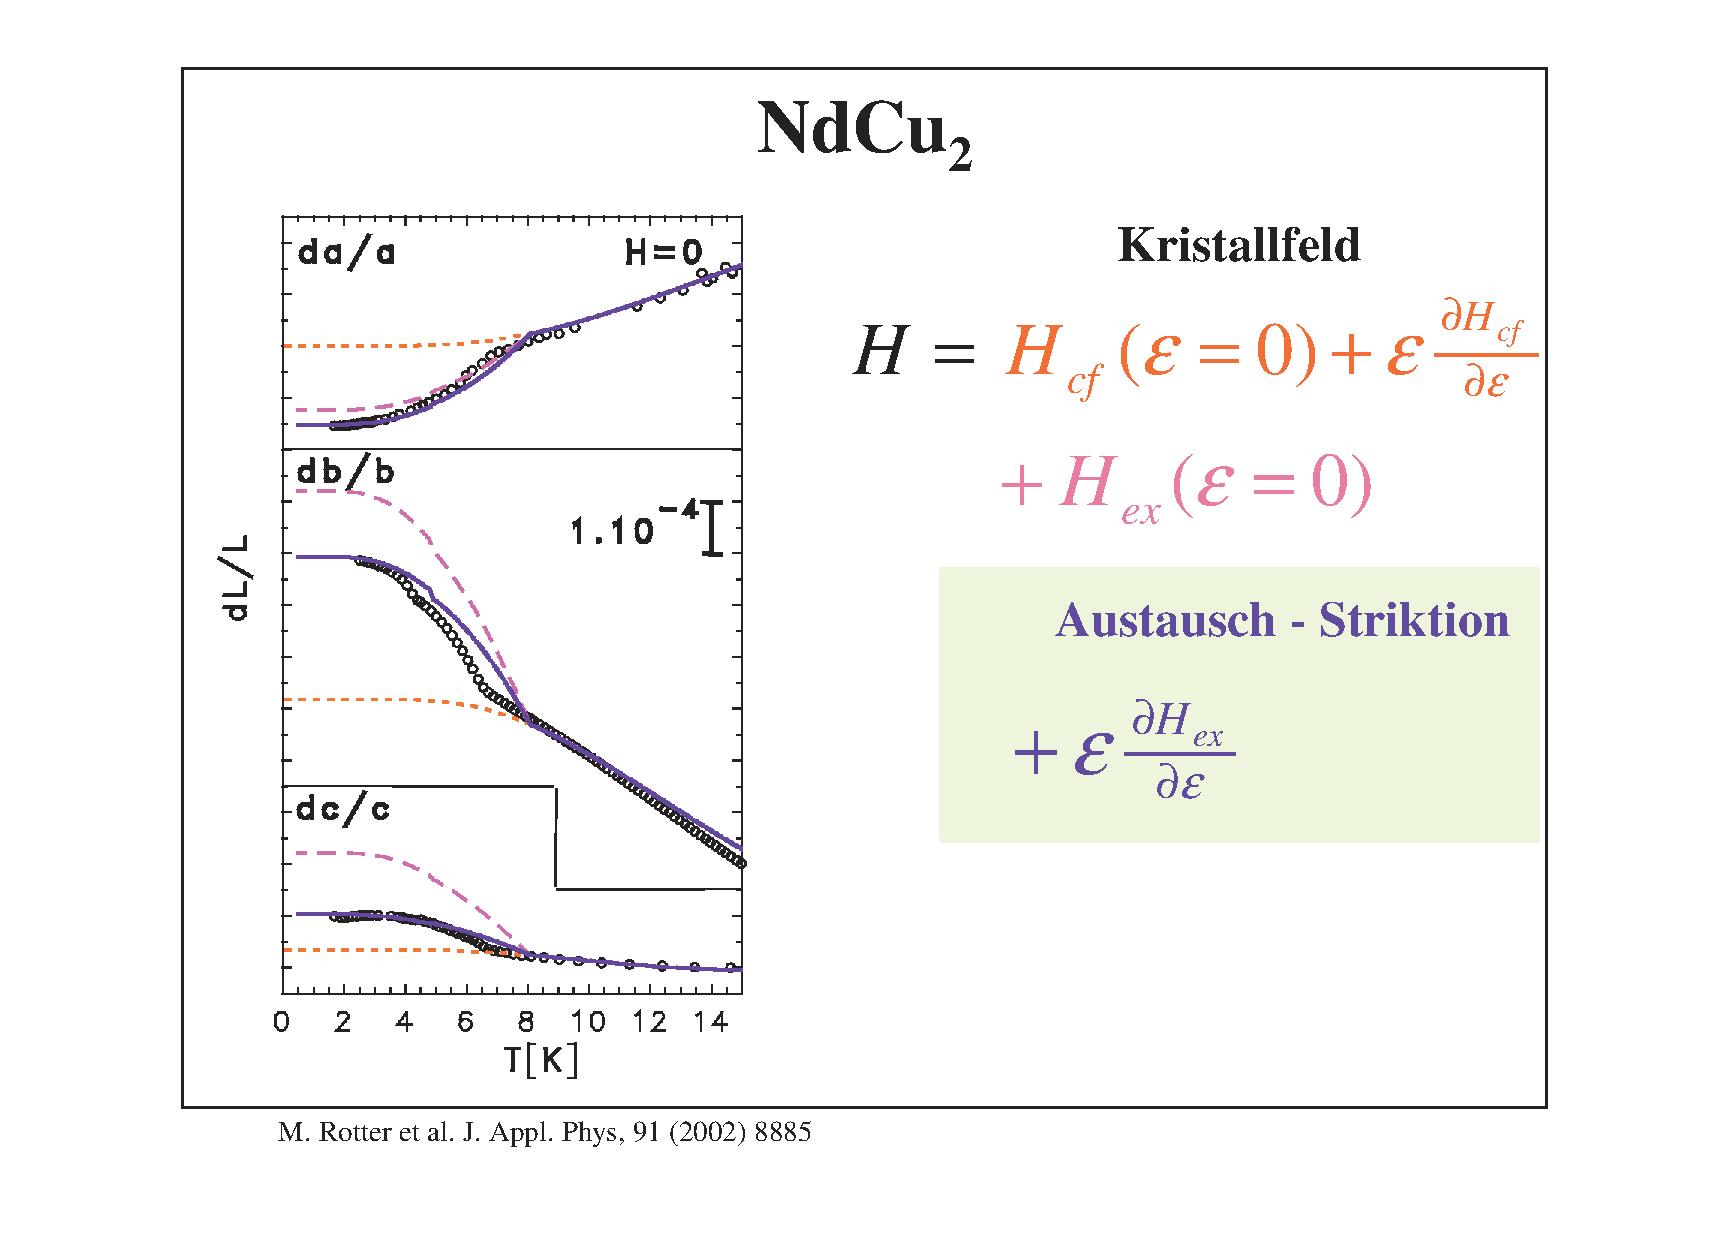
\includegraphics[angle=0, width=0.8\textwidth]{figsrc/magnetostriction_ndcu2.eps}
\end{center}
\caption{Calculated spontaneous magnetostriction of NdCu$_2$.}
\label{magnetostrictiongraphic}
\end{figure}

\begin{description}
\item [\prg mcphas.qvc]    the set of test q-vectors used for calculation of free energy.
                           Components of these q vectors refer to the reciprocal lattice $\vec a^*,\vec b^*,\vec c^*$.
\item [\prg mcphas.phs]    spin-configuration table of different types of spin-configurations. 
                            Note, in case of non-orthogonal axes the convention in these tables 
                            is $mb||\vec b$, $mc||(\vec a \times \vec b)$ and $ma$ perpendicular to $mb$ and $mc$.

                           {\em Note}: 
                           there is no natural criteria for deciding, if one spin-configuration is
			   different from another one. Therefore the list of ''different''
			   spin-configurations is dependent on the meaning of ''different''.
			   
			   The program {\prg McPhase} decides whether a spin-configuration is
			   different from another by a simple criteria, namely by the
			   angle between the spins. Comparing two spin configurations it calculates
			   the angle between corresponding spins and if for one spin the
			   angle is not small, the configuration is treated as a different
			   configuration. Therefore for example a ferromagnet with moments
			   in $a$ has a different spin configuration than a ferromagnet with
			   moments in $b$ direction. 
\item [\prg mcphas.sps]    $T-H$ dependence of spin-configuration. The spin configurations stored in this
                           file may be displayed using the program {\prg spins\index{spins}}, an example is given
			   in figure~\ref{spingraphic}.
                            Note, in case of non-orthogonal axes the convention for applied field $Ha, Hb,Hc$ and
                            also for the moment components $ma, mb, mc$ in these tables 
                            is $mb||\vec b$, $mc||(\vec a \times \vec b)$ and $ma$ perpendicular to $mb$ and $mc$.

\item [\prg mcphas.mf]     $T-H$ dependence of exchange field configuration, stored as $g_J \mu_B H_{xc}(i)$(unit is in meV)
                            for i=1,2,...,number of spins in magnetic unit cell.
                            Note, in case of non-orthogonal axes the convention for applied field $Ha, Hb,Hc$ and
                            also for the mean field components in these tables 
                            is $Hb||\vec b$, $Hc||(\vec a \times \vec b)$ and $Ha$ perpendicular to $Hb$ and $Hc$.
\item [\prg mcphas.fum]    free energy, magnetic energy (the derivative with respect to temperature gives the specific %%@
heat),
                           magnetisation data and (if cfield is used with higher order interactions)
                           expectation values of the Stevens Operators $<O_l^m>$ . As an example for the information
			   contained in this file the calculated magnetisation and magnetostriction of NdCu$_2$ is shown in
			   figures~\ref{magnetization} and ~\ref{magnetizationgraphic}.
                            Note, in case of non-orthogonal axes the convention for applied field $Ha, Hb,Hc$ and
                            also for the magnetisation components $ma,mb,mc$ in these tables 
                            is $Hb||\vec b$, $Hc||(\vec a \times \vec b)$ and $Ha$ perpendicular to $Hb$ and $Hc$.

\item [\prg mcphas1.j1 .j1 .j2 ...] 
               spin-spin correlation functions for sub-lattice 1 neighbour 1 2 ...
	       (linear combination is proportional to magnetostriction)
	       The spin-spin correlation functions for neighbour $k$ are defined by
	       the following sum of dyadic products:

	       \begin{equation}
	        \frac{1}{n}\sum_{s=1}^n <{\mbf J}^s> \times  <{\mbf J}^{s+k}>
	       \end{equation}
	       with $n$ being the number of moments in the magnetic unit cell.
	       Single ion and two-ion magnetostriction can be calculated using the $<O_l^m>$ and the
	       spin-spin correlation functions. As an example the magnetostriction analysis of
	       NdCu$_2$ is shown in figure~\ref{magnetostrictiongraphic}. For details 
             please refer to~\cite{rotter02-8885}.
                            Note, in case of non-orthogonal axes the convention for applied field $Ha, Hb,Hc$ and
                            also for the moment components in these tables 
                            is $Hb||\vec b$, $Hc||(\vec a \times \vec b)$ and $Ha$ perpendicular to $Hb$ and $Hc$.
\item [\prg mcphas.xyt]    phase diagram as x,y,T, H, phase-number j according to spin-configuration table
               given in mcphas.phs, a periodicity key, nettomoments <J>.
 Figure~\ref{phasediagramgraphic}
	       shows the phase diagram of NdCu$_2$ for magnetic fields parallel to the orthorhombic $b$-direction.
                            Note, in case of non-orthogonal axes the convention for applied field $Ha, Hb,Hc$ 
                             in these tables 
                            is $Hb||\vec b$, $Hc||(\vec a \times \vec b)$ and $Ha$ perpendicular to $Hb$ and $Hc$.
\item [\prg mcphas.hkl]    calculated (unpolarised) neutron diffraction data (the calculated magnetic intensities
    correspond to the magnetic structure + Polarisation factor. The
    Lorentz-factor , magnetic form factor and  instrumental corrections are not calculated.)
 As an example figure~\ref{neutintgraphic}
    shows the calculated temperature dependence of magnetic amplitudes for NdCu$_2$.
                           $h,k,l$ refer to the reciprocal lattice $\vec a^*,\vec b^*,\vec c^*$.
                            Note, in case of non-orthogonal axes the convention for applied field $Ha, Hb,Hc$ 
                             in these tables 
                            is $Hb||\vec b$, $Hc||(\vec a \times \vec b)$ and $Ha$ perpendicular to $Hb$ and $Hc$.
    
\item [\prg mcphasa.hkl]    Fourier Transform of the $a$-component of the magnetic Moments.
                           $h,k,l$ refer to the reciprocal lattice $\vec a^*,\vec b^*,\vec c^*$.
                            Note, in case of non-orthogonal axes the convention for applied field $Ha, Hb,Hc$ and
                            the magnetic moment component in these tables 
                            is $Hb||\vec b$, $Hc||(\vec a \times \vec b)$ and $Ha$ perpendicular to $Hb$ and $Hc$.
\item [\prg mcphasb.hkl]    Fourier Transform of the $b$-component of the magnetic Moments.
                           $h,k,l$ refer to the reciprocal lattice $\vec a^*,\vec b^*,\vec c^*$.
                            Note, in case of non-orthogonal axes the convention for applied field $Ha, Hb,Hc$ and
                            the magnetic moment component in these tables 
                            is $Hb||\vec b$, $Hc||(\vec a \times \vec b)$ and $Ha$ perpendicular to $Hb$ and $Hc$.
\item [\prg mcphasc.hkl]    Fourier Transform of the $c$-component of the magnetic Moments.
                           $h,k,l$ refer to the reciprocal lattice $\vec a^*,\vec b^*,\vec c^*$.
                            Note, in case of non-orthogonal axes the convention for applied field $Ha, Hb,Hc$ and
                            the magnetic moment component in these tables 
                            is $Hb||\vec b$, $Hc||(\vec a \times \vec b)$ and $Ha$ perpendicular to $Hb$ and $Hc$.
\end{description} 

\vspace{1cm}
{\em Exercises:}
\begin{itemize}
\item Look at the output files of {\prg McPhase}  in the directory
{\prg examples/ndcu2b\_new/results}.  At which magnetic field
the ferromagnetically aligned state is achieved (at $T=$2~K)?
\item
What is the propagation vector in the different antiferromagnetic phases at $T=$2~K ?
\end{itemize}



\subsubsection{{\prg mcphas.tst\index{mcphas.tst}} - input file of test spin-configurations (optional)}
This file is optional and contains
some test momentum configurations to be used for the calculation
             of the free energy. Mind that
\begin{itemize}
\item  in the file header the number of atoms in the primitive
       crystallographic unit cell and the number of components
       of the spin vector have to be given.
\item  at the end of the
 file there must be no empty lines !
\end{itemize}

The momentum - configurations tables always refer to spins sitting on
the primitive lattice ${\mbf r}_i$. If more than one atom is in
the primitive basis, the momentum gets $3n$ components ($n=$ number
of atoms in the crystallographic basis). See {\prg ./examples/ndcu2b\_new/} for
examples of a two atom basis. Units of these tables are that of total 
angular momentum $<J>$.

\subsubsection{Example {\prg mcphas.tst\index{mcphas.tst}} file  for a simple antiferromagnet}

Here is the file {\prg mcphas.tst\index{mcphas.tst}} for the simple antiferromagnet example
describing some spin configurations
to be used as starting values for the mean field process:

\section{{\prg mcphas} - calculation of thermodynamic properties (Magnetisation, Susceptibility, Specific Heat, Neutron %%@
Diffraction, etc.)}
\label{runmcphas}

In order to perform calculations beyond the capabilities of {\prg cfield\index{cfield}} it is necessary
to use the program {\prg mcphas}. 
\begin{itemize}
\item As a first step it is possible to
calculate the thermodynamic properties such as magnetisation or specific heat
considering only single ion effects. In this case all the exchange parameters
have to be set to zero in {\prg mcphas.j\index{mcphas.j}}. 
\item for more advanced calculations the two - ion interactions have to be
considered and may lead to magnetic order. {\prg mcphas} can perform 
calculations in the ordered state in the following way: for 
a given temperature $T$ and magnetic field $\mbf H$ (vector)
several possible magnetic structures are stabilised
by a mean field algorithm and the free energy is 
calculated. The initial values for this mean-field procedure are
modified by a Monte Carlo process.


The temperature and magnetic field is varied during the calculation
and thereby it is possible to map out the magnetic phase diagram.
\end{itemize}

The program produces a plot of the stabilised magnetic
structures and the magnetisation on screen, the
output files contain additional information 
such as calculated magnetoelastic and  neutron-scattering
data. Several graphic programs easy the visualisation of the
calculated data (section~\ref{graphics}).



\subsection{Input Files}
The program {\prg McPhase} needs the following input files (all in the same directory)
 in order to run:

\begin{enumerate}
\item {\prg mcphas.ini\index{mcphas.ini}}
 - controlling the algorithm
\item {\prg mcphas.j\index{mcphas.j}}
  - lattice and exchange parameters
\item {\prg mcphas.tst\index{mcphas.tst}(optional)}  - test spin configurations
\item {\prg single-ion property files}
\item {\prg directory ./results/}
 - directory where calculated data is stored
\item {\prg directory ./fit} - experimental data for fit (optional)
\end{enumerate}


 All
 of these input files have to be in one directory and the program
has to be started in this directory. The results of the simulation
are then stored in the  subdirectory ./results/, which must exist before starting
the program 
... see directory ./examples/ for some examples.
 In order to prepare these files
for a new calculation it is best to take them from an example, copy the files
to a new directory and make the
modifications  to adapt them to the new problem.

\subsubsection{Example - a simple antiferromagnet}

In the following description of the input files we will always refer
to a simple example: a simple antiferromagnet
on a primitive orthorhombic lattice. The first time user
will thus have a simple example to follow, all corresponding
files are given in the directory {\prg tutorial/03magnetic\_phases\_mcphas/simpleAF}.
 

\subsubsection{{\prg mcphas.ini\index{mcphas.ini}} - controlling the algorithm}
   Initial file containing algorithm control parameters, for instance the range and spacing of
   propagation vectors Q or the number of Monte Carlo trials for initial spin configurations
    - {\em mind}: this
   file is rewritten and reread  when running the program and may be changed by the
   user in order to manipulate the running simulation.

{\prg mcphas.ini\index{mcphas.ini}} consists of several sections:
\begin{description}
\item [MCPHASE RUNTIME CONTROL:] this section contains the parameters
controlling the status of the calculation.
\item [XY PHASEDIAGRAM PARAMETERS:] here the temperature and field range and
step widths of the calculation are specified.
The definition of the x and y
axis in terms of temperature and magnetic field is followed by the
corresponding range and step width. An offset may be given for all
field and temperature values.
Note that for most cases of interest
this offset is zero (T0=0, Ha0=0, Hb0=0, Hc0=0).
 For the simple case of calculating a Temperature-Field phase diagram
 It is just necessary to set xT=1 and give the temperature range by
xmin/xmax/xstep. For field in b direction then just set yHb=1 and 
define the range in ymin/ymax/ystep.
In case of non-orthogonal axes the applied magnetic field
components $Ha, Hb, Hc$ refer to the orthogonal coordinate system
defined with respect to the nonorthogonal lattice $\mbf a,\mbf b,\mbf c$ as
$Hb||\mbf b$, $Hc||(\mbf a \times \mbf b)$ and $Ha$ perpendicular to $Hb$ and $Hc$.

\item [GENERATION OF SPINCONFIGURATIONS:] at the beginning of the program
some initial values of spin configurations are generated from a set of 
propagation vectors. This section defines the range of propagation vectors
and the step width.
Depending on the value of the propagation Q with respect to the primitive reciprocal lattice
1-, 2- or 3-dimensional simulations of magnetic lattices
are possible. It is advisable to 
think carefully about the chosen range and spacing of Q vectors in order
to limit calculation time.
 
For example a good starting point is to begin with a calculation with large
step widths (e.g. 0.1)  covering the Brillouin zone. This should give an idea
of the propagation vectors which are stabilised. An advanced calculation
could then fine tune the propagation and determine its accurate value (using
small step widths in a limited area of the zone).
The verbose option of {\prg mcphas} allows to inspect the propagation vectors
which are actually used in the calculation.
Trick: in order to get a quick overview of the
q-vector range covered by the mcphas\index{mcphas} simulation start mcphas, exit and 
just type {\prg felog ./results/mcphas.qvc} (need {\prg perl,perldl,pdl,pgplot} packages).

In order to limit calculation time, the maximum periodicity
of the magnetic unit cell with respect to the crystallographic unit cell 
(maxqperiod) and the maximum number of spins in the magnetic unit cell 
(maxnofspins) can be limited. Also the maximum number of test spin configurations
in the internal table can be limited (maxnoftestspincf).
A critical feature with respect to calculation time is also the number of
spin configurations which are generated by a random process from a tabulated
SPINCONFIGURATIONS during the calculation. 

In summary the variables in this section are mainly important to adapt the
program to a given computer system with finite speed. They have to be set
to optimise between speed and accuracy of the calculation. In order to
find appropriate values it is best to perform some calculations 
and restrict the parameters step by step if insufficient speed is obtained.
Also the examples included in the program package may serve as starting
points.

\item [PARAMETERS FOR SUB FECALC SELFCONSISTENCY PROCESS:] the most important
procedure in the module {\prg mcphas} is the sub fecalc. In this part of the 
program the self consistent calculation of the magnetic moment configuration
is performed as shown schematically in fig.~\ref{fecalc}. 
In the mean field approximation the Hamiltonian~(\ref{hamilton}) is approximated
by

\begin{equation}
 {\mathcal H}=\sum_n H_{SI}^n + E_{corr}
\end{equation}

with the single ion Hamiltonian (in case of module {\prg so1ion\index{so1ion}})

\begin{equation}
H_{SI}^n=  B_l^m O_{lm}({\mbf J}^n) 
	     - g_{Jn} \mu_B {\mbf J}^n {\mbf H^n_{eff}} 
\end{equation}

and the correction term

\begin{equation}
E_{corr}=\frac{1}{2}\sum_{n} g_{Jn} \mu_B \langle {\mbf J}^n
 \rangle (\mbf H^n_{eff}-\mbf H) 
\end{equation}

and with the mean fields $ \mbf H^n_{eff}$ given by

\begin{equation}\label{meanfield}
\mbf H^n_{eff}=\mbf H + \mbf H^n_{xc}=\mbf H+\sum_{{\mbf G'}n'} \frac{{\mathcal J}
(\mbf r_n-(\mbf G'+\mbf r_{n'}))}{g_{Jn}\mu_B } \langle{\mbf
J}^{n'}\rangle
\end{equation}

These mean fields and the moments $\langle \mbf J^n \rangle$ 
are determined in a self consistent
way. For a given magnetic unit cell and initial configuration 
of magnetic moments
the mean fields are calculated according to equation~(\ref{meanfield}). 
Then, for each
magnetic ion the single ion property module is taken 
and the magnetic moment $\langle \mbf J^n \rangle$ is 
calculated from it's mean field. The mean fields are used again in equation~(\ref{meanfield})
and so on .... until convergence is reached. 
Then, the free energy ($f=-kT\sum_n \ln(z_n) + E_{corr}$ ) 
of the stabilised
configuration is calculated (this is why this sub is called {\prg fecalc}). 
The free energies of a lot of different stabilised configurations have to
be compared in order to find out which configuration has lowest free energy, i.e.
is stable in thermal  equilibrium.

It may happen that this process does
not converge due to bad choice of the initial configuration, therefore a maximum number
of mean field loops has to be given by the user.
The results of a calculation may be significantly influenced by
changing parameters such as the maximum number of iteration loops 
in this section. 
In fact the simulation is always a compromise of calculation time and accuracy: if only
a few initial spin configurations are tried at each (H-T) point, the calculation speed is
fast, however it is possible that the program misses the magnetic structure with the
lowest free energy. The same holds if other critical parameters of the simulation are
restricted too much.
 

\item [OUTPUT OF PHYSICAL PROPERTIES:]
Some options for the output of the calculation can be changed in this section.
\end{description}

\begin{figure}[hb]
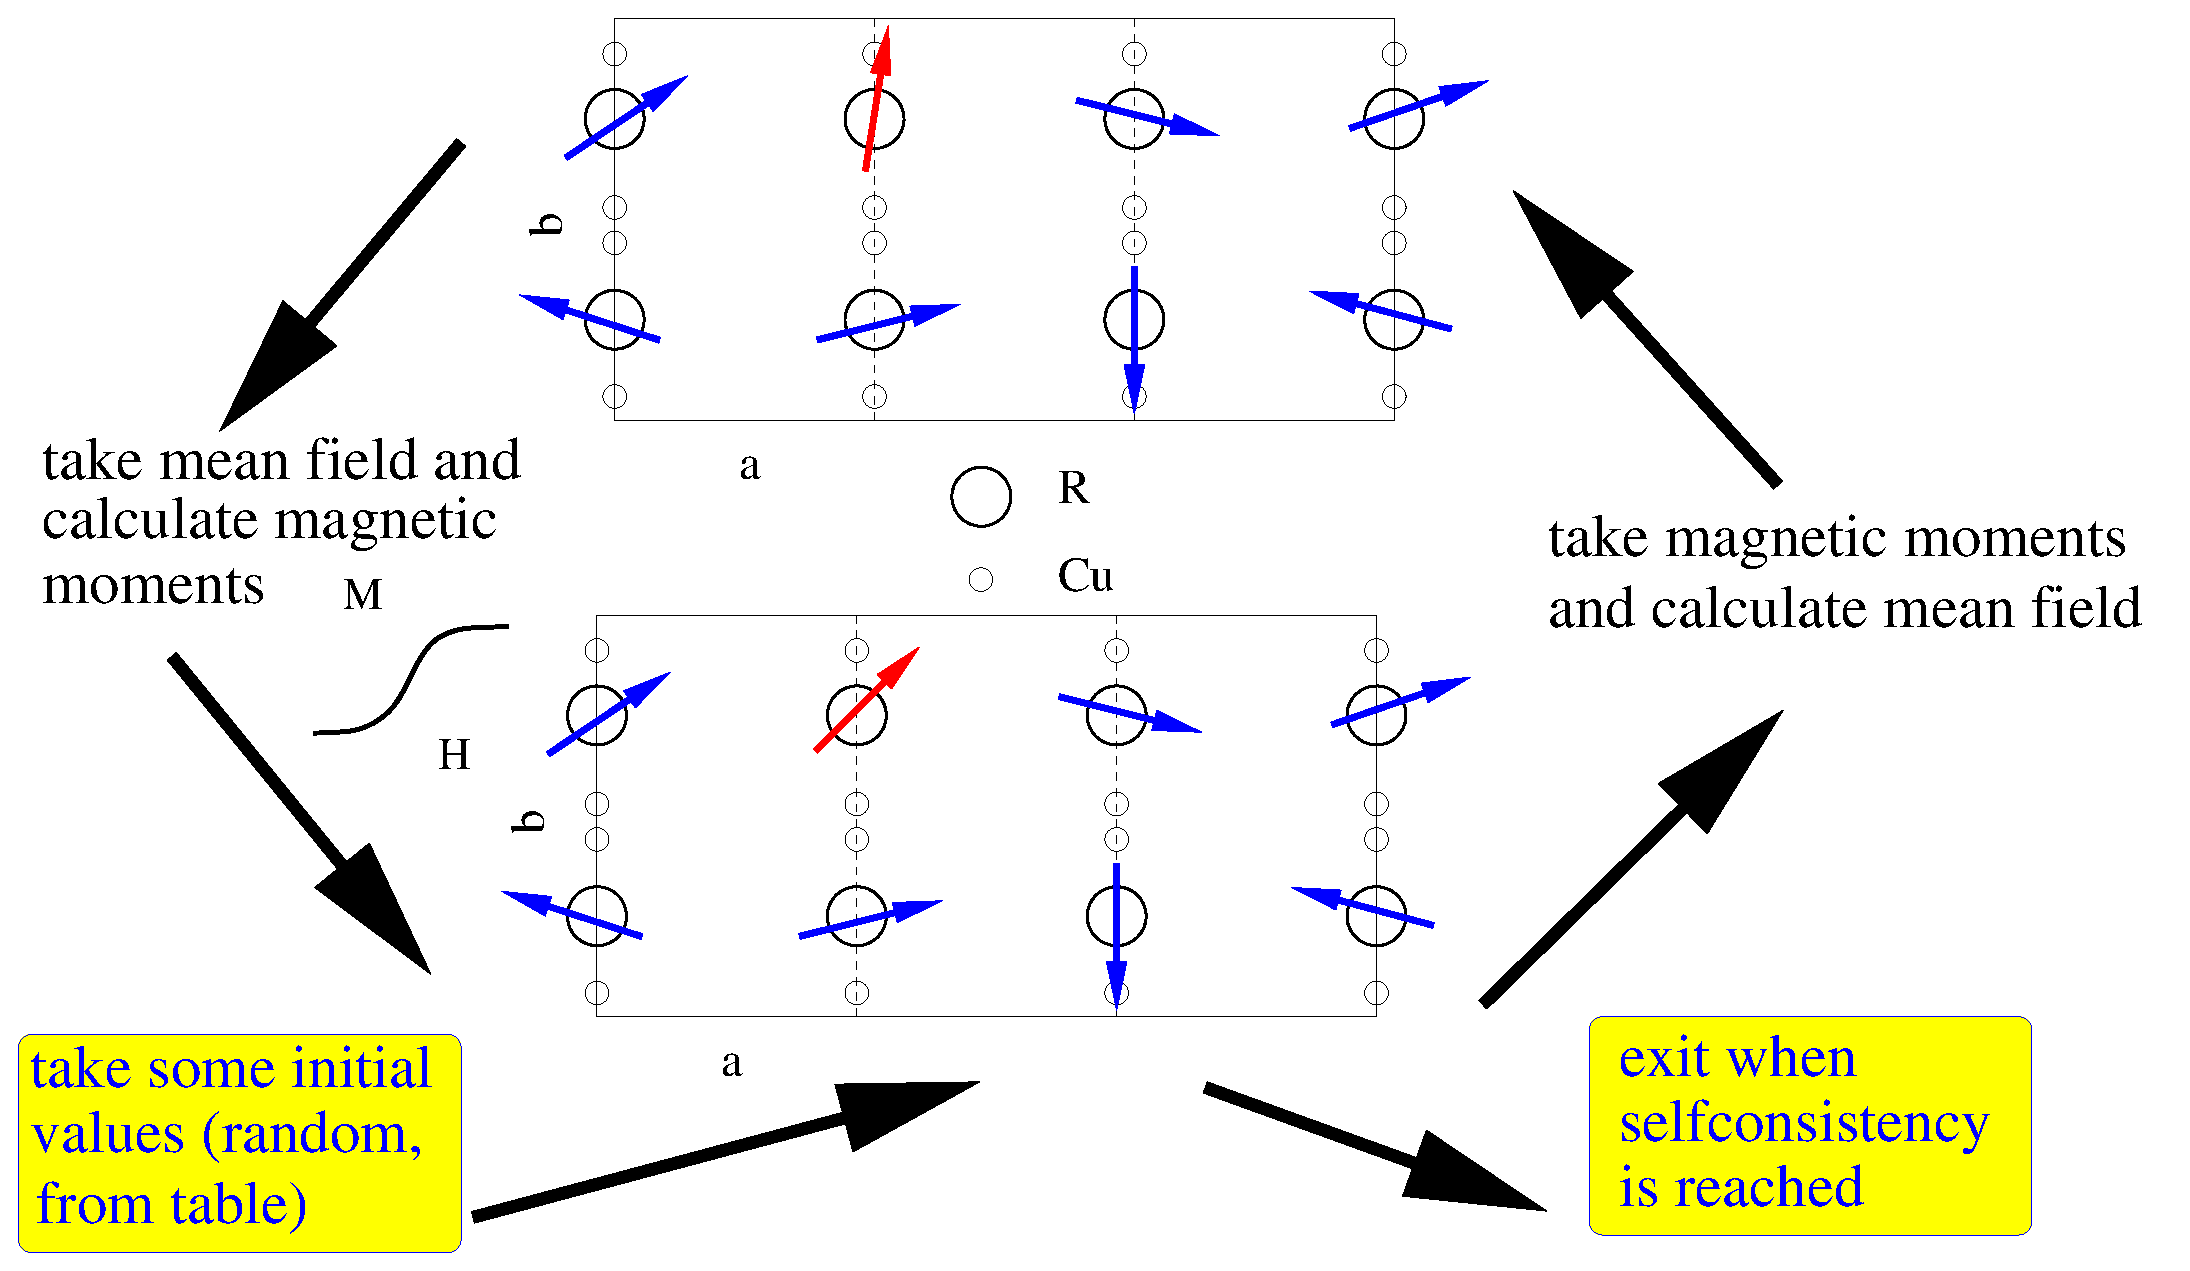
\includegraphics[angle=0,width=0.9\columnwidth]{figsrc/fecalc.eps}
\caption{\label{fecalc}Mean field process of sub {\prg fecalc}.}
\end{figure}

 
\subsubsection{Example {\prg mcphas.ini\index{mcphas.ini}} file for a simple antiferromagnet}

Here is an example of {\prg mcphas.ini\index{mcphas.ini}}, the comments describe the meaning of the different
parameters:

\input{mcphas.ini}



\subsubsection{{\prg mcphas.j\index{mcphas.j}} - lattice and exchange parameters}\label{mcphasj}
This file provides the information about 
the crystallographic
 structure and the magnetic exchange interactions.
For every atom in the crystallographic basis there
has to be given the coordinates, the number of neighbours to be considered, the 
Land\'e factor $g_J$, the single ion property filename and  a set of exchange parameters.
If the exchange parameters (and neighbour positions) are not known for your system, you 
can use the program module {\prg makenn\index{makenn}} (see section \ref{addprog}) to generate 
a list of nearest neighbours and
exchange parameters, currently implemented in {\prg makenn\index{makenn}} are dipolar interactions,
exchange interactions via the Bethe-Slater curve or the RKKY model. Note that in order
to use {\prg makenn\index{makenn}} you have to set up a working {\prg mcphas.j\index{mcphas.j}} file, which may or
may not contain neighbours and interactions.

Use program {\prg addj\index{addj}} to add exchange parameter set stored in different 
such {\prg .j} files (see section~\ref{addprog}).



\begin{description}
\item [Line 1,2:] Comment Lines
\item [Line 3:] lattice constants a,b,c and crystal angles alpha, beta, gamma 
\item [Line 4-6:] primitive lattice vectors
\item [Line 7:] Number of atoms in the primitive crystallographic unit cell ({\prg nofatoms})
\item [Line 8:] a comment line with stars
\item [Line 9:] coordinates  ($d_a$,$d_b$,$d_c$) of 1$^{st}$ magnetic ion in the crystallographic unit cell  with
respect to the lattice vectors $\vec a$,$\vec b$,$\vec c$. The number of neighbours of this 
ion, for which interaction constants are given in the interaction table (nofneighbours). 
If {\prg diagonalexchange}
is set to 0 the 9 components of the exchange tensor are given in column 4-12. 
If {\prg diagonalexchange}
 is 1, only 3 components are given (column 4-6).
If {\prg diagonalexchange}
 is 2, specific components of the exchange tensor can be given in columns 4 onwards. The indices of these components
 must be given in the following line (Line 9a below).
The Land\'e factor of the ion (gJ) and the file name of the corresponding single ion
parameter file (cffilename).
\item [Line 9a:]  If {\prg diagonalexchange=2}, then this line gives the indices of the exchange tensor corresponding to 
 the columns 4 onwards. It must have a variable called {\prg indexexchange} followed by a list of names of components of the interaction
 tensor separated by space. E.g.
 \verb|  #! indexexchange= JaJb JbJc  | 
means column 4 gives the the interaction constant between the
 first angular momentum component of the current ion with the second angular momentum component of its neighbour, whilst 
 column 5 has the interaction constant between the second angular momentum component of this ion with the third component of its
 neighbour. Alternatively, pairs of numbers may be given, as in \verb|  #! indexexchange= 1,2 2,3  |
 Additionally another parameter {\prg symmetricexchange} can be set to 1, where the value in each column is also used 
 for the transposed tensor component. Thus \verb|  #! symmetricexchange=1 indexexchange= JaJb  | is the same as \\
 \verb|  #! indexexchange= JaJb JbJa  | where the 4th and 5th column are the same.
\item [Line 10:]  Comment line
\item [Line 11-(10+nofneighbours):] Interaction table for ion number 1.   
Note: the neighbour coordinates (column 1-3) are given with respect to the lattice vectors
$\vec a$,$\vec b$,$\vec c$. The program then calculates from these values the coordinates
with respect to the primitive lattice $\vec r_1$,~$\vec r_2$,~$\vec r_3$.
($ d_a \vec a + d_b \vec b + d_c \vec c = d_1 \vec r_1 + d_2 \vec r_2 + d_3 \vec r_3$).
Column 4,5,6 \dots contain the components of the interaction tensor $\stackrel{=}{\mathcal J}$. 
Note that in case of non-orthogonal axes the 
components of the moments and the interaction tensor $Ja, Jb, Jc, Jaa, Jbb, Jcc, Jab ...$ 
refer to the orthogonal coordinate system
defined with respect to the nonorthogonal lattice $\vec a,\vec b,\vec c$ as
$Jb||\vec b$, $Jc||(\vec a \times \vec b)$ and $Ja$ perpendicular to $Jb$ and $Jc$.
\item [Line (11+nofneighbours) - end:] for each ion in the unit cell line 8 - (10+nofneighbours)
are repeated.
\end{description}


\vspace{0.5cm}

{\small {\bf Information for experienced users:}
\begin{description}
\item[\prg mcphas.jjj:]
format of exchange parameter file, which only needs a reduced set of exchange
parameters in the input file. Using the program {\prg jjj2j} the file can be transformed
to {\prg mcphas.j\index{mcphas.j}} by adding lines for all the equivalent neighbours. The format definition
of {\prg mcphas.jjj} is the same as {\prg mcphas.j\index{mcphas.j}}, however each line denotes several
equivalent neighbour atoms (instead of only one in {\prg mcphas.j\index{mcphas.j}}) according to the
 following rules:
\begin{itemize}
\item If a nonzero coordinate $d_a$ (or $d_b$,$d_c$) in the interaction table
 corresponds to it's value at the nearest
 lattice point of the primitive lattice,
  additional interactions of the same size
with  neighbours with coordinate $-d_a$ (or $-d_b$,$-d_c$, respectively)
are taken into account. This
holds for each of the three coordinates $d_a$,$d_b$ and $d_c$
 resulting in a maximum
number of 8 equivalent neighbours per line in the interaction table.
\item If the value of $d_a$ (or $d_b$,$d_c$) is zero or differs
from it's value at the nearest lattice point of the primitive lattice, it is 
changed to the value at the nearest lattice point and {\bf no} interaction 
with  neighbours with coordinates $-d_a$ (or $-d_b$,$-d_c$) is
 taken into account. If such
 interaction is needed it may be given in a different line and may
have different magnitude. In this way also crystallographic lattices
with no mirror symmetry may be described.
\end{itemize}
\item[\prg mcphas.coq:]   exchange parameters etc [ in old format]...see examples for details, use {\prg coq2jjj} to 
transform {\prg mcphas.coq} to {\prg mcphas.jjj} format
\end{description}

}


\subsubsection{Example {\prg mcphas.j\index{mcphas.j}} file for a simple antiferromagnet}

Here are example files of a tetragonal antiferromagnet with nearest neighbour interactions, all
files are equivalent:

{\small
\begin{verbatim} 
# simple antiferromagnet 
#<!--mcphase.mcphas.j-->
#***************************************************************
# Lattice Constants (A)
#! a=4.3843 b=4.3843 c=2.4194 alpha=  90 beta=  90 gamma=  90
#! r1a=   1 r2a=   0 r3a=   0
#! r1b=   0 r2b=   1 r3b=   0   primitive lattice vectors [a][b][c]
#! r1c=   0 r2c=   0 r3c=   1
#! nofatoms=1  nofcomponents=3  number of atoms in primitive unit cell/number of components of each spin
# ****************************************************************************
#! da=  0 [a] db=  0 [b] dc=  0 nofneighbours=2 diagonalexchange=0 gJ=0.857143 cffilename=Ce3p.sipf
# da[a] db[b] dc[c] Jaa[meV] Jbb[meV] Jcc[meV] Jab[meV] Jba[meV] Jac[meV] Jca[meV] Jbc[meV] Jcb[meV]
+0	+0	+1	-0.1	-0.1	-0.1   0  0  0  0  0  0
+0	+0	-1	-0.1	-0.1	-0.1   0  0  0  0  0  0
#\end{verbatim}
}

Using diagonalexchange this may be shortened to

{\small
\begin{verbatim} 
# simple antiferromagnet 
#<!--mcphase.mcphas.j-->
#***************************************************************
# Lattice Constants (A)
#! a=4.3843 b=4.3843 c=2.4194 alpha=  90 beta=  90 gamma=  90
#! r1a=   1 r2a=   0 r3a=   0
#! r1b=   0 r2b=   1 r3b=   0   primitive lattice vectors [a][b][c]
#! r1c=   0 r2c=   0 r3c=   1
#! nofatoms=1  nofcomponents=3  number of atoms in primitive unit cell/number of components of each spin
# ****************************************************************************
#! da=  0 [a] db=  0 [b] dc=  0 nofneighbours=2 diagonalexchange=1 gJ=0.857143 cffilename=Ce3p.sipf
# da[a] db[b] dc[c] Jaa[meV] Jbb[meV] Jcc[meV] Jab[meV] Jba[meV] Jac[meV] Jca[meV] Jbc[meV] Jcb[meV]
+0	+0	+1	-0.1	-0.1	-0.1   
+0	+0	-1	-0.1	-0.1	-0.1   
#\end{verbatim}
}

with indexexchange option the sequence of two ion interaction parameters can be changed and
zero parameters may be omitted:

{\small
\begin{verbatim} 
# simple antiferromagnet 
#<!--mcphase.mcphas.j-->
#***************************************************************
# Lattice Constants (A)
#! a=4.3843 b=4.3843 c=2.4194 alpha=  90 beta=  90 gamma=  90
#! r1a=   1 r2a=   0 r3a=   0
#! r1b=   0 r2b=   1 r3b=   0   primitive lattice vectors [a][b][c]
#! r1c=   0 r2c=   0 r3c=   1
#! nofatoms=1  nofcomponents=3  number of atoms in primitive unit cell/number of components of each spin
# ****************************************************************************
#! da=  0 [a] db=  0 [b] dc=  0 nofneighbours=2 diagonalexchange=2 gJ=0.857143 cffilename=Ce3p.sipf
# da[a] db[b] dc[c] Jaa[meV] Jbb[meV] Jcc[meV] Jab[meV] Jba[meV] Jac[meV] Jca[meV] Jbc[meV] Jcb[meV]
#! indexexchange = JaJa JaJc JcJa JbJb JcJc
+0	+0	+1	-0.1 0 0 -0.1	-0.1  
+0	+0	-1	-0.1 0 0 -0.1	-0.1  
#\end{verbatim}
}

{\small
\begin{verbatim} 
# simple antiferromagnet 
#<!--mcphase.mcphas.j-->
#***************************************************************
# Lattice Constants (A)
#! a=4.3843 b=4.3843 c=2.4194 alpha=  90 beta=  90 gamma=  90
#! r1a=   1 r2a=   0 r3a=   0
#! r1b=   0 r2b=   1 r3b=   0   primitive lattice vectors [a][b][c]
#! r1c=   0 r2c=   0 r3c=   1
#! nofatoms=1  nofcomponents=3  number of atoms in primitive unit cell/number of components of each spin
# ****************************************************************************
#! da=  0 [a] db=  0 [b] dc=  0 nofneighbours=2 diagonalexchange=2 gJ=0.857143 cffilename=Ce3p.sipf
# da[a] db[b] dc[c] Jaa[meV] Jbb[meV] Jcc[meV] Jab[meV] Jba[meV] Jac[meV] Jca[meV] Jbc[meV] Jcb[meV]
#! indexexchange = 1,1 1,3, 3,1 2,2 3,3
+0	+0	+1	-0.1 0 0 -0.1	-0.1  
+0	+0	-1	-0.1 0 0 -0.1	-0.1  
#\end{verbatim}
}


using symmetricexchange together with indexexchange will assume that the interaction tensor is symmetic and 
only half of it may be given:

{\small
\begin{verbatim} 
# simple antiferromagnet 
#<!--mcphase.mcphas.j-->
#***************************************************************
# Lattice Constants (A)
#! a=4.3843 b=4.3843 c=2.4194 alpha=  90 beta=  90 gamma=  90
#! r1a=   1 r2a=   0 r3a=   0
#! r1b=   0 r2b=   1 r3b=   0   primitive lattice vectors [a][b][c]
#! r1c=   0 r2c=   0 r3c=   1
#! nofatoms=1  nofcomponents=3  number of atoms in primitive unit cell/number of components of each spin
# ****************************************************************************
#! da=  0 [a] db=  0 [b] dc=  0 nofneighbours=2 diagonalexchange=2 gJ=0.857143 cffilename=Ce3p.sipf
# da[a] db[b] dc[c] Jaa[meV] Jbb[meV] Jcc[meV] Jab[meV] Jba[meV] Jac[meV] Jca[meV] Jbc[meV] Jcb[meV]
#! symmetricexchange=1 indexexchange = JaJa JaJc JbJb JcJc
+0	+0	+1	-0.1 0  -0.1	-0.1  
+0	+0	-1	-0.1 0  -0.1	-0.1  
#\end{verbatim}
}


\subsubsection{Single Ion Property Input Files}\label{sifile}

In order to speed up calculations or treat special problems a large 
variety of single ion modules is available. This includes the
option to load a user written single ion module. Details are 
given in chapter~\ref{simod}.

The first time user of {\prg McPhase} should use the module {\prg so1ion}\index{so1ion} and 
create an appropriate single ion property input file as described in
section \ref{cf1ion}. A good starting point are several examples
given in directory {\prg examples}.


\subsubsection{Example single ion property file  for a simple antiferromagnet}

Here is an example file {\prg mcphas.cf1} describing the anisotropy of a 
simple antiferromagnet with Ce atoms having basal plane anisotropy. Note the
axis convention xyz$||$abc, in case of non-orthogonal axes the convention 
is $y||\vec b$, $z||(\vec a \times \vec b)$ and $x$ perpendicular to $y$ and $z$.


\input{mcphas.cf1}

\subsubsection{{\prg mcphas.tst\index{mcphas.tst}} - input file of test spin-configurations (optional)}
This file is optional and contains
some test momentum configurations to be used for the calculation
             of the free energy. Mind that
\begin{itemize}
\item  in the file header the number of atoms in the primitive
       crystallographic unit cell and the number of components
       of the spin vector have to be given.
\item  at the end of the
 file there must be no empty lines !
\end{itemize}

The momentum - configurations tables always refer to spins sitting on
the primitive lattice ${\mbf r}_i$. If more than one atom is in
the primitive basis, the momentum gets $3n$ components ($n=$ number
of atoms in the crystallographic basis). See {\prg ./examples/ndcu2b\_new/} for
examples of a two atom basis. Units of these tables are that of total 
angular momentum $<J>$.

\subsubsection{Example {\prg mcphas.tst\index{mcphas.tst}} file  for a simple antiferromagnet}

Here is the file {\prg mcphas.tst\index{mcphas.tst}} for the simple antiferromagnet example
describing some spin configurations
to be used as starting values for the mean field process:

\input{mcphas.tst}
Note, in case of non-orthogonal axes the convention 
is $mb||\vec b$, $mc||(\vec a \times \vec b)$ and $ma$ perpendicular to $mb$ and $mc$.

\subsubsection{subdirectory {\prg ./results} - directory where calculated data is stored}

In order to be able to save the results of a calculation the directory {\prg ./results} has to
exist. Mind that all files in this directory will be overwritten without warning. 

\subsubsection{subdirectory {\prg ./fit} - experimental data for fit (optional) } 

In order that {\prg McPhase} can calculate the standard deviation between
 experimental data and the results of the simulation, some experimental data
 can be given in the subdirectory {\prg ./fit}. The filenames and the data-format
 are the same as the output files of {\prg McPhas}, e.g. {\prg mcphas.fum}, {\prg mcphas.hkl}
 etc. {\prg McPhase} looks into the directory {\prg ./fit} and if it finds any
 of these files, the standard deviation is increased correspondingly. 

What measurement data can be used to calculate a standard deviation ?

\begin{description}
\item[{\prg mcphas.fum}] if given in column 11, 12, 13 in {\prg ./fit/mcphas.fum} the
            magnetisation in the $a$, $b$ and $c$ direction is used for calculation
	    of the standard deviation sta. The standard deviation is calculated
	    as ${\rm sta}=\sum_{\rm data points i} ({\mbf m}_i^{calc}-{\mbf m}_i^{meas})^2$.
	    All three components of the magnetic moment have to be given and are used.

\end{description}

Note that the measured data has to be given in those (H-T) points which are 
calculated by mcphas\index{mcphas} in order to be used by the program to increase {\prg sta}.
It is usually most effective to fit only few data points, because a large set
of data points will not improve the quality of the fit and only require a large
amount of calculation time.



\subsection{Starting a simulation}
\label{start}

To start the simulation goto the directory containing the
input files {\prg mcphas.ini, mcphas.j, etc. } and type

\begin{description}
\item[\prg mcphas] to run the program generating stepwise $H-T$ values 
              in a loop given by {\prg mcphas.ini\index{mcphas.ini}} (you can also press the
              symbol in the {\prg McPhase - Explorer} window).
\item[\prg mcphas\index{mcphas} [file]]  to run the program with an input file --   
             {\prg file} contains T ha hb hc values to be calculated 
             if [file] is not given, xmin xmax xstep (xT xHa xHb xHc)
             ymin ymax ystep (yT yHa yHb yHc) is read from file {\prg mcphas.ini\index{mcphas.ini}}
	     and phase diagram is calculated
\item[\prg mcphas\index{mcphas} -h]  to  print help and version of {\prg McPhas}.
\item[\prg mcphas\index{mcphas} -stamax 14]  end mcphas\index{mcphas} if standard deviation exceeds 14.
\item[\prg mcphas\index{mcphas} -a] avoid overwriting output files in results, append new results to existing files
\item[\prg mcphas\index{mcphas} -v]  to  enable verbose mode with lots of messages of {\prg McPhas}. Specifically
the verbose mode enables the following features:
  \begin{itemize}
			          \item more information is printed out, 
			          \item the q-vectors file {\prg ./results/mcphas.qvc} will contain 
				    the explicit spin configurations
			          \item the display\index{display} on screen (ghostview window using 
				     {\prg ./results/.sps.eps}) will be updated not only 
				    when a H-T point has been finished but always 
				    when a structure with smaller free energy 
				    has been stabilised
  \end{itemize}
\item[\prg mcphasit\index{mcphas}] to start mcphase in commandline mode without opening any window
\end{description}

\vspace{1cm}
{\em Exercises:}
\begin{itemize}
\item Look at the input files for {\prg McPhase} given in the directory
{\prg examples/ndcu2b\_new}.  How many atoms are contained in the crystallographic basis ?
\item
Start the simulation by typing the command {\prg mcphas}.
\end{itemize}



\subsection{Options for a running simulation}
... when the program is running, the options in the main window
can be changed. Pressing ''displayall'' displays the current spin-configuration
at each iteration step. Pressing ''log fe vs Q'' appends free energy vs Q
data to {\prg mcphas.log} for every ($T-H$) point.


The file {\prg ./results/.spins.eps} is used to show the information about the currently calculated
spin structure on the screen using the postscript file viewer ghostview.

The file {\prg ./results/.mcphas.fum} contains the information of the magnetisation curve
which is currently calculated. This information is automatically displayed on the screen.


The program {\prg display} (see section \ref{display}) can be used 
for the online display\index{display} of any other
curve(s).


\subsection{Output Files - {\prg mcphas.qvc,phs,sps,mf,fum,j1...,xyt,hkl} }\label{outputfiles}
 (in directory ./results/ after a simulation run) 

\begin{figure}[htb]%h=here, t=top, b=bottom, p=separate figure page
\begin{center}\leavevmode
\includegraphics[angle=0, width=0.3\textwidth]{figsrc/magnetization_ndcu2.ps}
\end{center}
\caption{Calculated magnetisation of NdCu$_2$ for field parallel to the orthorhombic $b$-direction.}
\label{magnetization}
\end{figure}

\begin{figure}[htb]%h=here, t=top, b=bottom, p=separate figure page
\begin{center}\leavevmode
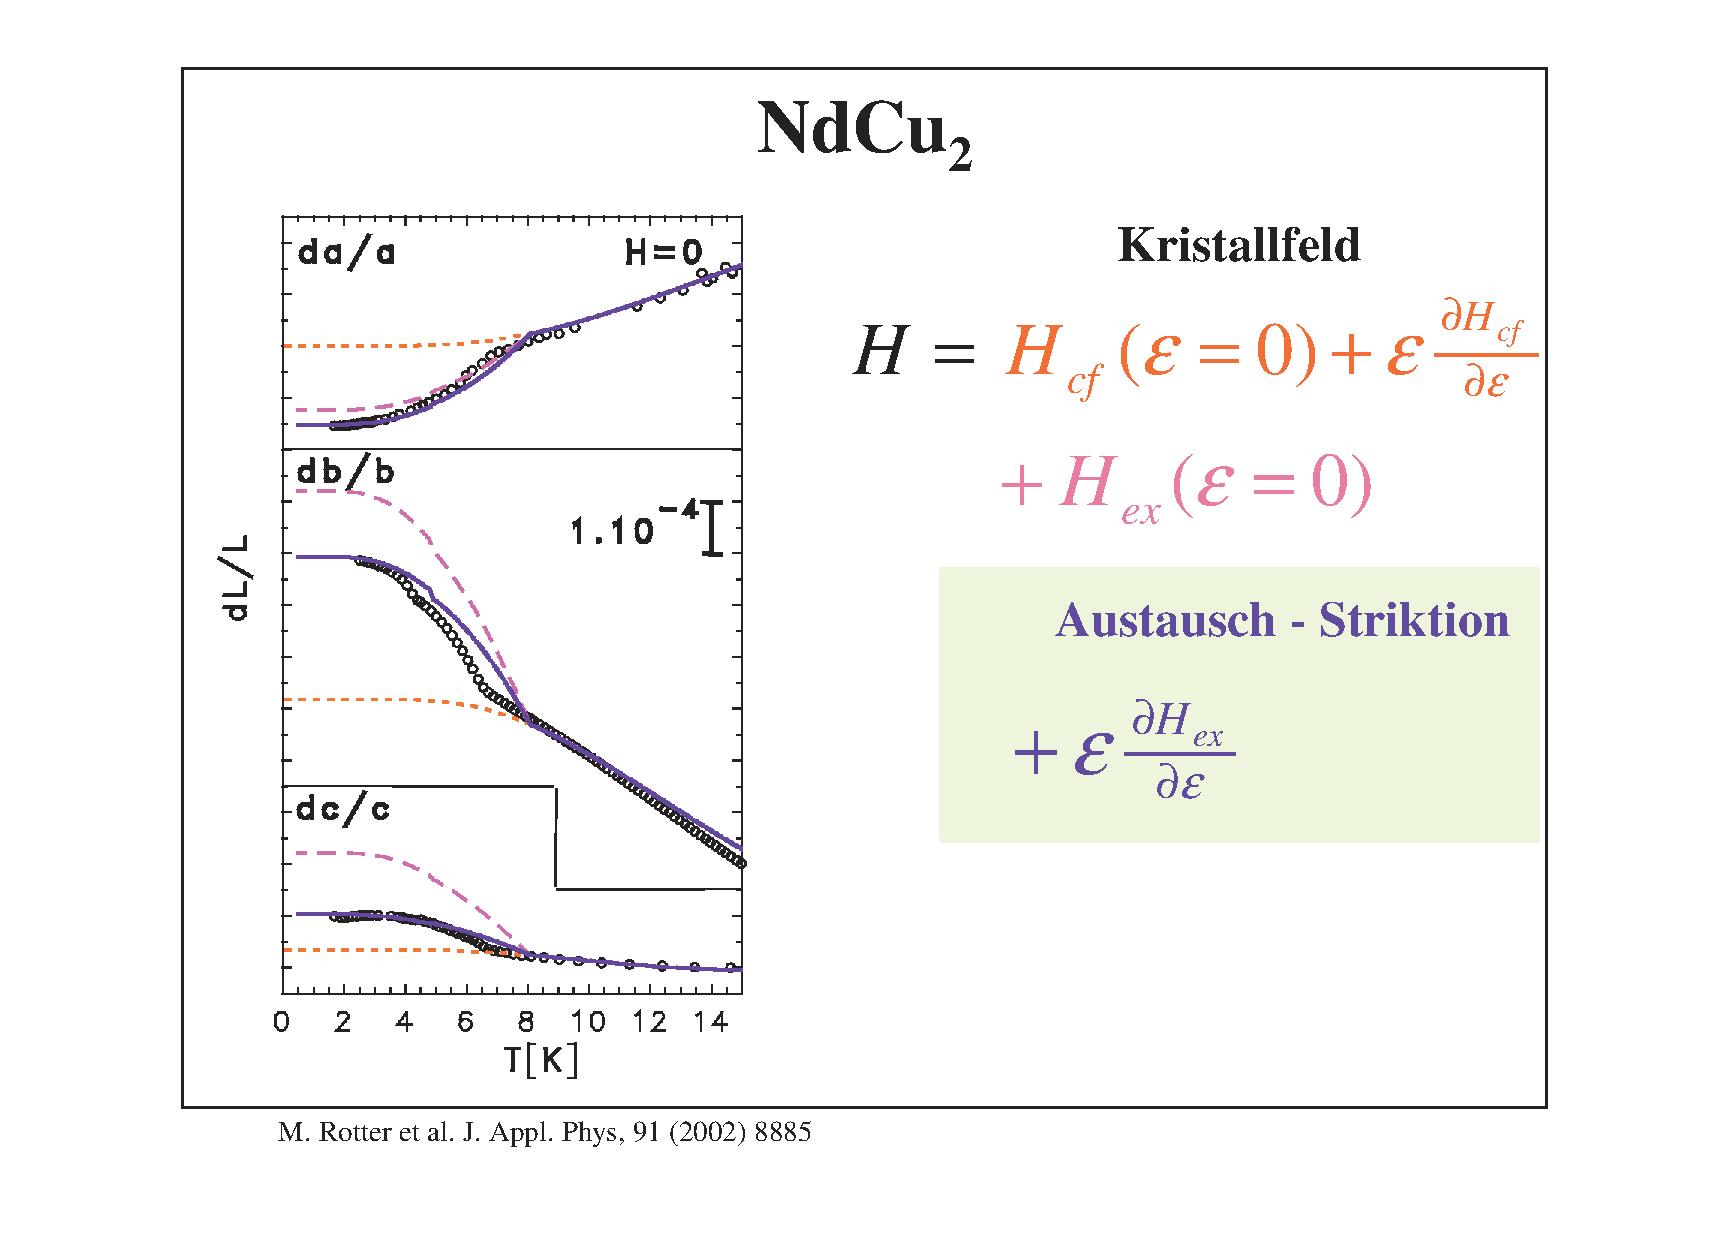
\includegraphics[angle=0, width=0.8\textwidth]{figsrc/magnetostriction_ndcu2.eps}
\end{center}
\caption{Calculated spontaneous magnetostriction of NdCu$_2$.}
\label{magnetostrictiongraphic}
\end{figure}

\begin{description}
\item [\prg mcphas.qvc]    the set of test q-vectors used for calculation of free energy.
                           Components of these q vectors refer to the reciprocal lattice $\vec a^*,\vec b^*,\vec c^*$.
\item [\prg mcphas.phs]    spin-configuration table of different types of spin-configurations. 
                            Note, in case of non-orthogonal axes the convention in these tables 
                            is $mb||\vec b$, $mc||(\vec a \times \vec b)$ and $ma$ perpendicular to $mb$ and $mc$.

                           {\em Note}: 
                           there is no natural criteria for deciding, if one spin-configuration is
			   different from another one. Therefore the list of ''different''
			   spin-configurations is dependent on the meaning of ''different''.
			   
			   The program {\prg McPhase} decides whether a spin-configuration is
			   different from another by a simple criteria, namely by the
			   angle between the spins. Comparing two spin configurations it calculates
			   the angle between corresponding spins and if for one spin the
			   angle is not small, the configuration is treated as a different
			   configuration. Therefore for example a ferromagnet with moments
			   in $a$ has a different spin configuration than a ferromagnet with
			   moments in $b$ direction. 
\item [\prg mcphas.sps]    $T-H$ dependence of spin-configuration. The spin configurations stored in this
                           file may be displayed using the program {\prg spins\index{spins}}, an example is given
			   in figure~\ref{spingraphic}.
                            Note, in case of non-orthogonal axes the convention for applied field $Ha, Hb,Hc$ and
                            also for the moment components $ma, mb, mc$ in these tables 
                            is $mb||\vec b$, $mc||(\vec a \times \vec b)$ and $ma$ perpendicular to $mb$ and $mc$.

\item [\prg mcphas.mf]     $T-H$ dependence of exchange field configuration, stored as $g_J \mu_B H_{xc}(i)$(unit is in meV)
                            for i=1,2,...,number of spins in magnetic unit cell.
                            Note, in case of non-orthogonal axes the convention for applied field $Ha, Hb,Hc$ and
                            also for the mean field components in these tables 
                            is $Hb||\vec b$, $Hc||(\vec a \times \vec b)$ and $Ha$ perpendicular to $Hb$ and $Hc$.
\item [\prg mcphas.fum]    free energy, magnetic energy (the derivative with respect to temperature gives the specific %%@
heat),
                           magnetisation data and (if cfield is used with higher order interactions)
                           expectation values of the Stevens Operators $<O_l^m>$ . As an example for the information
			   contained in this file the calculated magnetisation and magnetostriction of NdCu$_2$ is shown in
			   figures~\ref{magnetization} and ~\ref{magnetizationgraphic}.
                            Note, in case of non-orthogonal axes the convention for applied field $Ha, Hb,Hc$ and
                            also for the magnetisation components $ma,mb,mc$ in these tables 
                            is $Hb||\vec b$, $Hc||(\vec a \times \vec b)$ and $Ha$ perpendicular to $Hb$ and $Hc$.

\item [\prg mcphas1.j1 .j1 .j2 ...] 
               spin-spin correlation functions for sub-lattice 1 neighbour 1 2 ...
	       (linear combination is proportional to magnetostriction)
	       The spin-spin correlation functions for neighbour $k$ are defined by
	       the following sum of dyadic products:

	       \begin{equation}
	        \frac{1}{n}\sum_{s=1}^n <{\mbf J}^s> \times  <{\mbf J}^{s+k}>
	       \end{equation}
	       with $n$ being the number of moments in the magnetic unit cell.
	       Single ion and two-ion magnetostriction can be calculated using the $<O_l^m>$ and the
	       spin-spin correlation functions. As an example the magnetostriction analysis of
	       NdCu$_2$ is shown in figure~\ref{magnetostrictiongraphic}. For details 
             please refer to~\cite{rotter02-8885}.
                            Note, in case of non-orthogonal axes the convention for applied field $Ha, Hb,Hc$ and
                            also for the moment components in these tables 
                            is $Hb||\vec b$, $Hc||(\vec a \times \vec b)$ and $Ha$ perpendicular to $Hb$ and $Hc$.
\item [\prg mcphas.xyt]    phase diagram as x,y,T, H, phase-number j according to spin-configuration table
               given in mcphas.phs, a periodicity key, nettomoments <J>.
 Figure~\ref{phasediagramgraphic}
	       shows the phase diagram of NdCu$_2$ for magnetic fields parallel to the orthorhombic $b$-direction.
                            Note, in case of non-orthogonal axes the convention for applied field $Ha, Hb,Hc$ 
                             in these tables 
                            is $Hb||\vec b$, $Hc||(\vec a \times \vec b)$ and $Ha$ perpendicular to $Hb$ and $Hc$.
\item [\prg mcphas.hkl]    calculated (unpolarised) neutron diffraction data (the calculated magnetic intensities
    correspond to the magnetic structure + Polarisation factor. The
    Lorentz-factor , magnetic form factor and  instrumental corrections are not calculated.)
 As an example figure~\ref{neutintgraphic}
    shows the calculated temperature dependence of magnetic amplitudes for NdCu$_2$.
                           $h,k,l$ refer to the reciprocal lattice $\vec a^*,\vec b^*,\vec c^*$.
                            Note, in case of non-orthogonal axes the convention for applied field $Ha, Hb,Hc$ 
                             in these tables 
                            is $Hb||\vec b$, $Hc||(\vec a \times \vec b)$ and $Ha$ perpendicular to $Hb$ and $Hc$.
    
\item [\prg mcphasa.hkl]    Fourier Transform of the $a$-component of the magnetic Moments.
                           $h,k,l$ refer to the reciprocal lattice $\vec a^*,\vec b^*,\vec c^*$.
                            Note, in case of non-orthogonal axes the convention for applied field $Ha, Hb,Hc$ and
                            the magnetic moment component in these tables 
                            is $Hb||\vec b$, $Hc||(\vec a \times \vec b)$ and $Ha$ perpendicular to $Hb$ and $Hc$.
\item [\prg mcphasb.hkl]    Fourier Transform of the $b$-component of the magnetic Moments.
                           $h,k,l$ refer to the reciprocal lattice $\vec a^*,\vec b^*,\vec c^*$.
                            Note, in case of non-orthogonal axes the convention for applied field $Ha, Hb,Hc$ and
                            the magnetic moment component in these tables 
                            is $Hb||\vec b$, $Hc||(\vec a \times \vec b)$ and $Ha$ perpendicular to $Hb$ and $Hc$.
\item [\prg mcphasc.hkl]    Fourier Transform of the $c$-component of the magnetic Moments.
                           $h,k,l$ refer to the reciprocal lattice $\vec a^*,\vec b^*,\vec c^*$.
                            Note, in case of non-orthogonal axes the convention for applied field $Ha, Hb,Hc$ and
                            the magnetic moment component in these tables 
                            is $Hb||\vec b$, $Hc||(\vec a \times \vec b)$ and $Ha$ perpendicular to $Hb$ and $Hc$.
\end{description} 

\vspace{1cm}
{\em Exercises:}
\begin{itemize}
\item Look at the output files of {\prg McPhase}  in the directory
{\prg examples/ndcu2b\_new/results}.  At which magnetic field
the ferromagnetically aligned state is achieved (at $T=$2~K)?
\item
What is the propagation vector in the different antiferromagnetic phases at $T=$2~K ?
\end{itemize}


Note, in case of non-orthogonal axes the convention 
is $mb||\vec b$, $mc||(\vec a \times \vec b)$ and $ma$ perpendicular to $mb$ and $mc$.

\subsubsection{subdirectory {\prg ./results} - directory where calculated data is stored}

In order to be able to save the results of a calculation the directory {\prg ./results} has to
exist. Mind that all files in this directory will be overwritten without warning. 

\subsubsection{subdirectory {\prg ./fit} - experimental data for fit (optional) } 

In order that {\prg McPhase} can calculate the standard deviation between
 experimental data and the results of the simulation, some experimental data
 can be given in the subdirectory {\prg ./fit}. The filenames and the data-format
 are the same as the output files of {\prg McPhas}, e.g. {\prg mcphas.fum}, {\prg mcphas.hkl}
 etc. {\prg McPhase} looks into the directory {\prg ./fit} and if it finds any
 of these files, the standard deviation is increased correspondingly. 

What measurement data can be used to calculate a standard deviation ?

\begin{description}
\item[{\prg mcphas.fum}] if given in column 11, 12, 13 in {\prg ./fit/mcphas.fum} the
            magnetisation in the $a$, $b$ and $c$ direction is used for calculation
	    of the standard deviation sta. The standard deviation is calculated
	    as ${\rm sta}=\sum_{\rm data points i} ({\mbf m}_i^{calc}-{\mbf m}_i^{meas})^2$.
	    All three components of the magnetic moment have to be given and are used.

\end{description}

Note that the measured data has to be given in those (H-T) points which are 
calculated by mcphas\index{mcphas} in order to be used by the program to increase {\prg sta}.
It is usually most effective to fit only few data points, because a large set
of data points will not improve the quality of the fit and only require a large
amount of calculation time.



\subsection{Starting a simulation}
\label{start}

To start the simulation goto the directory containing the
input files {\prg mcphas.ini, mcphas.j, etc. } and type

\begin{description}
\item[\prg mcphas] to run the program generating stepwise $H-T$ values 
              in a loop given by {\prg mcphas.ini\index{mcphas.ini}} (you can also press the
              symbol in the {\prg McPhase - Explorer} window).
\item[\prg mcphas\index{mcphas} [file]]  to run the program with an input file --   
             {\prg file} contains T ha hb hc values to be calculated 
             if [file] is not given, xmin xmax xstep (xT xHa xHb xHc)
             ymin ymax ystep (yT yHa yHb yHc) is read from file {\prg mcphas.ini\index{mcphas.ini}}
	     and phase diagram is calculated
\item[\prg mcphas\index{mcphas} -h]  to  print help and version of {\prg McPhas}.
\item[\prg mcphas\index{mcphas} -stamax 14]  end mcphas\index{mcphas} if standard deviation exceeds 14.
\item[\prg mcphas\index{mcphas} -a] avoid overwriting output files in results, append new results to existing files
\item[\prg mcphas\index{mcphas} -v]  to  enable verbose mode with lots of messages of {\prg McPhas}. Specifically
the verbose mode enables the following features:
  \begin{itemize}
			          \item more information is printed out, 
			          \item the q-vectors file {\prg ./results/mcphas.qvc} will contain 
				    the explicit spin configurations
			          \item the display\index{display} on screen (ghostview window using 
				     {\prg ./results/.sps.eps}) will be updated not only 
				    when a H-T point has been finished but always 
				    when a structure with smaller free energy 
				    has been stabilised
  \end{itemize}
\item[\prg mcphasit\index{mcphas}] to start mcphase in commandline mode without opening any window
\end{description}

\vspace{1cm}
{\em Exercises:}
\begin{itemize}
\item Look at the input files for {\prg McPhase} given in the directory
{\prg examples/ndcu2b\_new}.  How many atoms are contained in the crystallographic basis ?
\item
Start the simulation by typing the command {\prg mcphas}.
\end{itemize}



\subsection{Options for a running simulation}
... when the program is running, the options in the main window
can be changed. Pressing ''displayall'' displays the current spin-configuration
at each iteration step. Pressing ''log fe vs Q'' appends free energy vs Q
data to {\prg mcphas.log} for every ($T-H$) point.


The file {\prg ./results/.spins.eps} is used to show the information about the currently calculated
spin structure on the screen using the postscript file viewer ghostview.

The file {\prg ./results/.mcphas.fum} contains the information of the magnetisation curve
which is currently calculated. This information is automatically displayed on the screen.


The program {\prg display} (see section \ref{display}) can be used 
for the online display\index{display} of any other
curve(s).


\subsection{Output Files - {\prg mcphas.qvc,phs,sps,mf,fum,j1...,xyt,hkl} }\label{outputfiles}
 (in directory ./results/ after a simulation run) 

\begin{figure}[htb]%h=here, t=top, b=bottom, p=separate figure page
\begin{center}\leavevmode
\includegraphics[angle=0, width=0.3\textwidth]{figsrc/magnetization_ndcu2.ps}
\end{center}
\caption{Calculated magnetisation of NdCu$_2$ for field parallel to the orthorhombic $b$-direction.}
\label{magnetization}
\end{figure}

\begin{figure}[htb]%h=here, t=top, b=bottom, p=separate figure page
\begin{center}\leavevmode
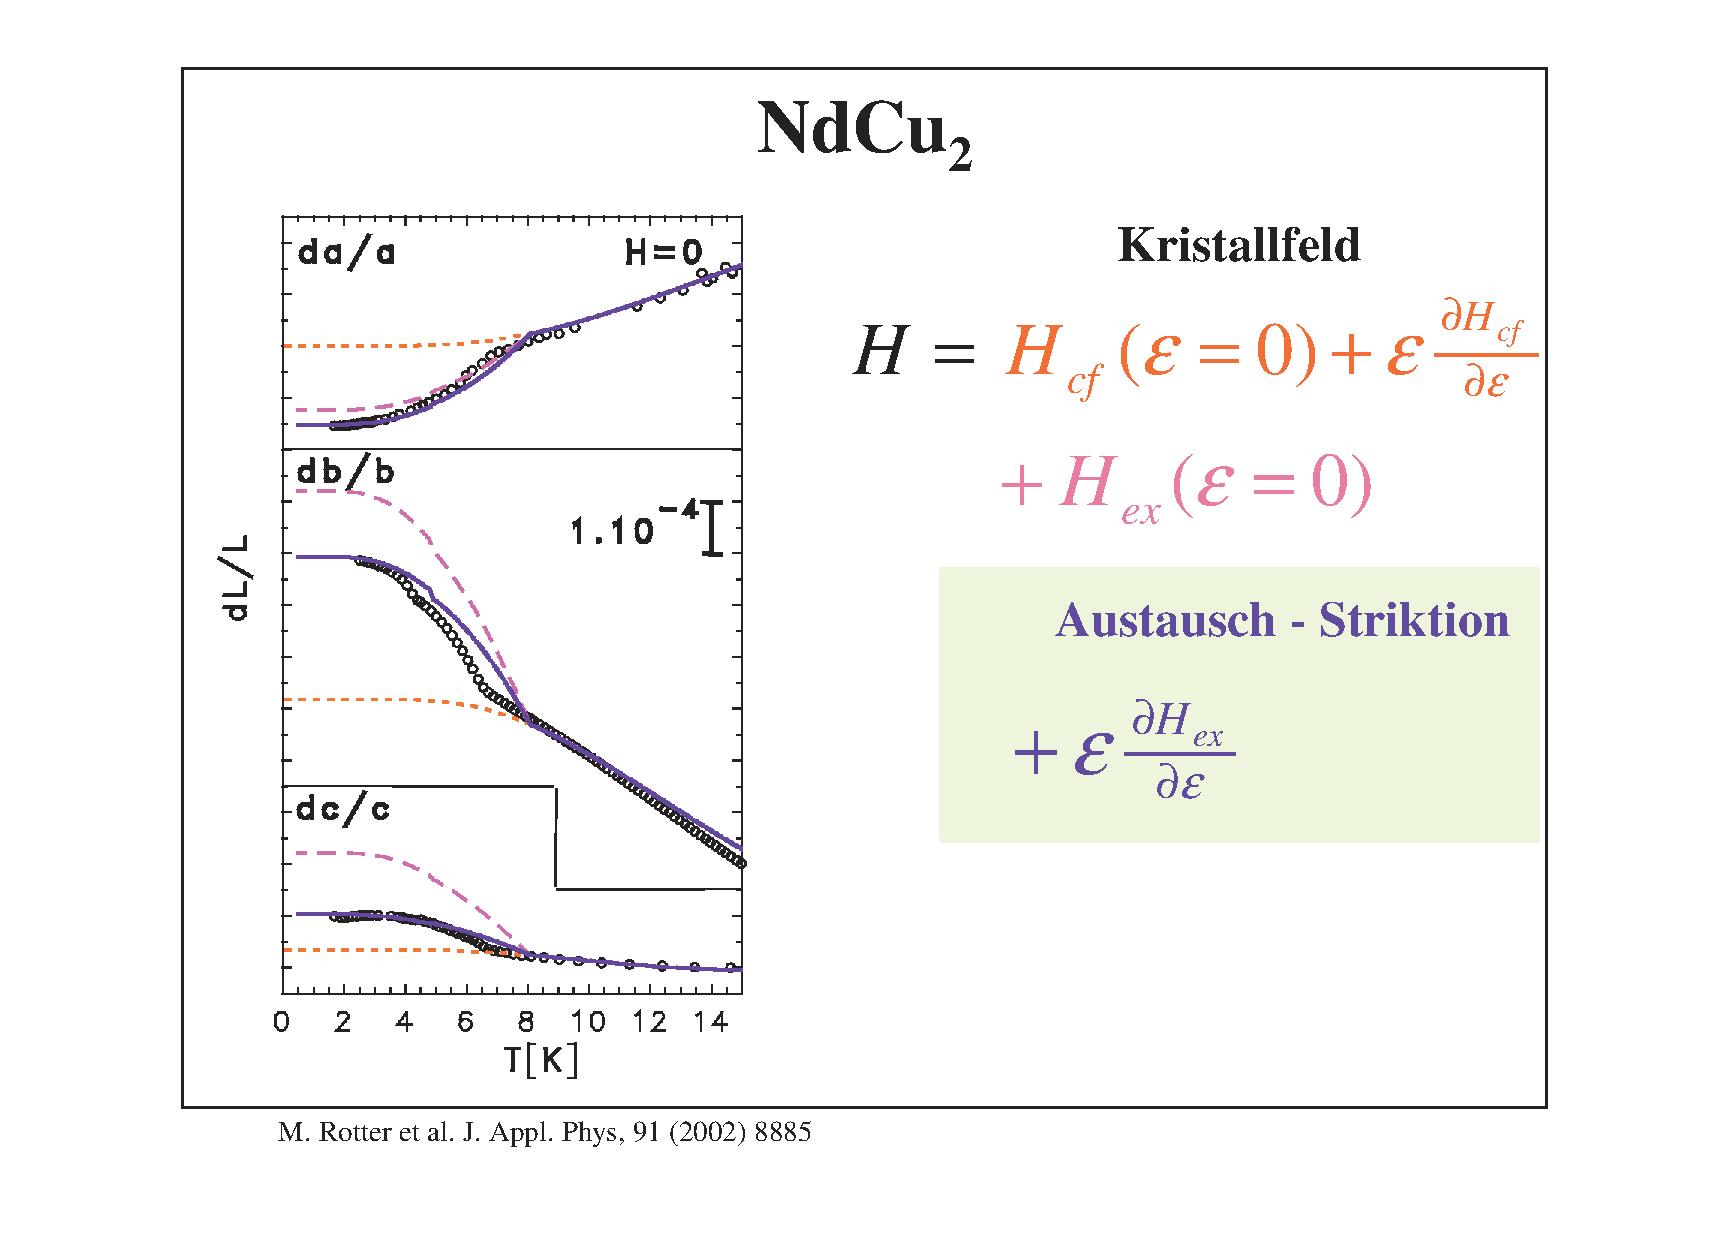
\includegraphics[angle=0, width=0.8\textwidth]{figsrc/magnetostriction_ndcu2.eps}
\end{center}
\caption{Calculated spontaneous magnetostriction of NdCu$_2$.}
\label{magnetostrictiongraphic}
\end{figure}

\begin{description}
\item [\prg mcphas.qvc]    the set of test q-vectors used for calculation of free energy.
                           Components of these q vectors refer to the reciprocal lattice $\vec a^*,\vec b^*,\vec c^*$.
\item [\prg mcphas.phs]    spin-configuration table of different types of spin-configurations. 
                            Note, in case of non-orthogonal axes the convention in these tables 
                            is $mb||\vec b$, $mc||(\vec a \times \vec b)$ and $ma$ perpendicular to $mb$ and $mc$.

                           {\em Note}: 
                           there is no natural criteria for deciding, if one spin-configuration is
			   different from another one. Therefore the list of ''different''
			   spin-configurations is dependent on the meaning of ''different''.
			   
			   The program {\prg McPhase} decides whether a spin-configuration is
			   different from another by a simple criteria, namely by the
			   angle between the spins. Comparing two spin configurations it calculates
			   the angle between corresponding spins and if for one spin the
			   angle is not small, the configuration is treated as a different
			   configuration. Therefore for example a ferromagnet with moments
			   in $a$ has a different spin configuration than a ferromagnet with
			   moments in $b$ direction. 
\item [\prg mcphas.sps]    $T-H$ dependence of spin-configuration. The spin configurations stored in this
                           file may be displayed using the program {\prg spins\index{spins}}, an example is given
			   in figure~\ref{spingraphic}.
                            Note, in case of non-orthogonal axes the convention for applied field $Ha, Hb,Hc$ and
                            also for the moment components $ma, mb, mc$ in these tables 
                            is $mb||\vec b$, $mc||(\vec a \times \vec b)$ and $ma$ perpendicular to $mb$ and $mc$.

\item [\prg mcphas.mf]     $T-H$ dependence of exchange field configuration, stored as $g_J \mu_B H_{xc}(i)$(unit is in meV)
                            for i=1,2,...,number of spins in magnetic unit cell.
                            Note, in case of non-orthogonal axes the convention for applied field $Ha, Hb,Hc$ and
                            also for the mean field components in these tables 
                            is $Hb||\vec b$, $Hc||(\vec a \times \vec b)$ and $Ha$ perpendicular to $Hb$ and $Hc$.
\item [\prg mcphas.fum]    free energy, magnetic energy (the derivative with respect to temperature gives the specific %%@
heat),
                           magnetisation data and (if cfield is used with higher order interactions)
                           expectation values of the Stevens Operators $<O_l^m>$ . As an example for the information
			   contained in this file the calculated magnetisation and magnetostriction of NdCu$_2$ is shown in
			   figures~\ref{magnetization} and ~\ref{magnetizationgraphic}.
                            Note, in case of non-orthogonal axes the convention for applied field $Ha, Hb,Hc$ and
                            also for the magnetisation components $ma,mb,mc$ in these tables 
                            is $Hb||\vec b$, $Hc||(\vec a \times \vec b)$ and $Ha$ perpendicular to $Hb$ and $Hc$.

\item [\prg mcphas1.j1 .j1 .j2 ...] 
               spin-spin correlation functions for sub-lattice 1 neighbour 1 2 ...
	       (linear combination is proportional to magnetostriction)
	       The spin-spin correlation functions for neighbour $k$ are defined by
	       the following sum of dyadic products:

	       \begin{equation}
	        \frac{1}{n}\sum_{s=1}^n <{\mbf J}^s> \times  <{\mbf J}^{s+k}>
	       \end{equation}
	       with $n$ being the number of moments in the magnetic unit cell.
	       Single ion and two-ion magnetostriction can be calculated using the $<O_l^m>$ and the
	       spin-spin correlation functions. As an example the magnetostriction analysis of
	       NdCu$_2$ is shown in figure~\ref{magnetostrictiongraphic}. For details 
             please refer to~\cite{rotter02-8885}.
                            Note, in case of non-orthogonal axes the convention for applied field $Ha, Hb,Hc$ and
                            also for the moment components in these tables 
                            is $Hb||\vec b$, $Hc||(\vec a \times \vec b)$ and $Ha$ perpendicular to $Hb$ and $Hc$.
\item [\prg mcphas.xyt]    phase diagram as x,y,T, H, phase-number j according to spin-configuration table
               given in mcphas.phs, a periodicity key, nettomoments <J>.
 Figure~\ref{phasediagramgraphic}
	       shows the phase diagram of NdCu$_2$ for magnetic fields parallel to the orthorhombic $b$-direction.
                            Note, in case of non-orthogonal axes the convention for applied field $Ha, Hb,Hc$ 
                             in these tables 
                            is $Hb||\vec b$, $Hc||(\vec a \times \vec b)$ and $Ha$ perpendicular to $Hb$ and $Hc$.
\item [\prg mcphas.hkl]    calculated (unpolarised) neutron diffraction data (the calculated magnetic intensities
    correspond to the magnetic structure + Polarisation factor. The
    Lorentz-factor , magnetic form factor and  instrumental corrections are not calculated.)
 As an example figure~\ref{neutintgraphic}
    shows the calculated temperature dependence of magnetic amplitudes for NdCu$_2$.
                           $h,k,l$ refer to the reciprocal lattice $\vec a^*,\vec b^*,\vec c^*$.
                            Note, in case of non-orthogonal axes the convention for applied field $Ha, Hb,Hc$ 
                             in these tables 
                            is $Hb||\vec b$, $Hc||(\vec a \times \vec b)$ and $Ha$ perpendicular to $Hb$ and $Hc$.
    
\item [\prg mcphasa.hkl]    Fourier Transform of the $a$-component of the magnetic Moments.
                           $h,k,l$ refer to the reciprocal lattice $\vec a^*,\vec b^*,\vec c^*$.
                            Note, in case of non-orthogonal axes the convention for applied field $Ha, Hb,Hc$ and
                            the magnetic moment component in these tables 
                            is $Hb||\vec b$, $Hc||(\vec a \times \vec b)$ and $Ha$ perpendicular to $Hb$ and $Hc$.
\item [\prg mcphasb.hkl]    Fourier Transform of the $b$-component of the magnetic Moments.
                           $h,k,l$ refer to the reciprocal lattice $\vec a^*,\vec b^*,\vec c^*$.
                            Note, in case of non-orthogonal axes the convention for applied field $Ha, Hb,Hc$ and
                            the magnetic moment component in these tables 
                            is $Hb||\vec b$, $Hc||(\vec a \times \vec b)$ and $Ha$ perpendicular to $Hb$ and $Hc$.
\item [\prg mcphasc.hkl]    Fourier Transform of the $c$-component of the magnetic Moments.
                           $h,k,l$ refer to the reciprocal lattice $\vec a^*,\vec b^*,\vec c^*$.
                            Note, in case of non-orthogonal axes the convention for applied field $Ha, Hb,Hc$ and
                            the magnetic moment component in these tables 
                            is $Hb||\vec b$, $Hc||(\vec a \times \vec b)$ and $Ha$ perpendicular to $Hb$ and $Hc$.
\end{description} 

\vspace{1cm}
{\em Exercises:}
\begin{itemize}
\item Look at the output files of {\prg McPhase}  in the directory
{\prg examples/ndcu2b\_new/results}.  At which magnetic field
the ferromagnetically aligned state is achieved (at $T=$2~K)?
\item
What is the propagation vector in the different antiferromagnetic phases at $T=$2~K ?
\end{itemize}


Note, in case of non-orthogonal axes the convention 
is $mb||\vec b$, $mc||(\vec a \times \vec b)$ and $ma$ perpendicular to $mb$ and $mc$.

\subsubsection{subdirectory {\prg ./results} - directory where calculated data is stored}

In order to be able to save the results of a calculation the directory {\prg ./results} has to
exist. Mind that all files in this directory will be overwritten without warning. 

\subsubsection{subdirectory {\prg ./fit} - experimental data for fit (optional) } 

In order that {\prg McPhase} can calculate the standard deviation between
 experimental data and the results of the simulation, some experimental data
 can be given in the subdirectory {\prg ./fit}. The filenames and the data-format
 are the same as the output files of {\prg McPhas}, e.g. {\prg mcphas.fum}, {\prg mcphas.hkl}
 etc. {\prg McPhase} looks into the directory {\prg ./fit} and if it finds any
 of these files, the standard deviation is increased correspondingly. 

What measurement data can be used to calculate a standard deviation ?

\begin{description}
\item[{\prg mcphas.fum}] if given in column 11, 12, 13 in {\prg ./fit/mcphas.fum} the
            magnetisation in the $a$, $b$ and $c$ direction is used for calculation
	    of the standard deviation sta. The standard deviation is calculated
	    as ${\rm sta}=\sum_{\rm data points i} ({\mbf m}_i^{calc}-{\mbf m}_i^{meas})^2$.
	    All three components of the magnetic moment have to be given and are used.

\end{description}

Note that the measured data has to be given in those (H-T) points which are 
calculated by mcphas\index{mcphas} in order to be used by the program to increase {\prg sta}.
It is usually most effective to fit only few data points, because a large set
of data points will not improve the quality of the fit and only require a large
amount of calculation time.



\subsection{Starting a simulation}
\label{start}

To start the simulation goto the directory containing the
input files {\prg mcphas.ini, mcphas.j, etc. } and type

\begin{description}
\item[\prg mcphas] to run the program generating stepwise $H-T$ values 
              in a loop given by {\prg mcphas.ini\index{mcphas.ini}} (you can also press the
              symbol in the {\prg McPhase - Explorer} window).
\item[\prg mcphas\index{mcphas} [file]]  to run the program with an input file --   
             {\prg file} contains T ha hb hc values to be calculated 
             if [file] is not given, xmin xmax xstep (xT xHa xHb xHc)
             ymin ymax ystep (yT yHa yHb yHc) is read from file {\prg mcphas.ini\index{mcphas.ini}}
	     and phase diagram is calculated
\item[\prg mcphas\index{mcphas} -h]  to  print help and version of {\prg McPhas}.
\item[\prg mcphas\index{mcphas} -stamax 14]  end mcphas\index{mcphas} if standard deviation exceeds 14.
\item[\prg mcphas\index{mcphas} -a] avoid overwriting output files in results, append new results to existing files
\item[\prg mcphas\index{mcphas} -v]  to  enable verbose mode with lots of messages of {\prg McPhas}. Specifically
the verbose mode enables the following features:
  \begin{itemize}
			          \item more information is printed out, 
			          \item the q-vectors file {\prg ./results/mcphas.qvc} will contain 
				    the explicit spin configurations
			          \item the display\index{display} on screen (ghostview window using 
				     {\prg ./results/.sps.eps}) will be updated not only 
				    when a H-T point has been finished but always 
				    when a structure with smaller free energy 
				    has been stabilised
  \end{itemize}
\item[\prg mcphasit\index{mcphas}] to start mcphase in commandline mode without opening any window
\end{description}

\vspace{1cm}
{\em Exercises:}
\begin{itemize}
\item Look at the input files for {\prg McPhase} given in the directory
{\prg examples/ndcu2b\_new}.  How many atoms are contained in the crystallographic basis ?
\item
Start the simulation by typing the command {\prg mcphas}.
\end{itemize}



\subsection{Options for a running simulation}
... when the program is running, the options in the main window
can be changed. Pressing ''displayall'' displays the current spin-configuration
at each iteration step. Pressing ''log fe vs Q'' appends free energy vs Q
data to {\prg mcphas.log} for every ($T-H$) point.


The file {\prg ./results/.spins.eps} is used to show the information about the currently calculated
spin structure on the screen using the postscript file viewer ghostview.

The file {\prg ./results/.mcphas.fum} contains the information of the magnetisation curve
which is currently calculated. This information is automatically displayed on the screen.


The program {\prg display} (see section \ref{display}) can be used 
for the online display\index{display} of any other
curve(s).


\subsection{Output Files - {\prg mcphas.qvc,phs,sps,mf,fum,j1...,xyt,hkl} }\label{outputfiles}
 (in directory ./results/ after a simulation run) 

\begin{figure}[htb]%h=here, t=top, b=bottom, p=separate figure page
\begin{center}\leavevmode
\includegraphics[angle=0, width=0.3\textwidth]{figsrc/magnetization_ndcu2.ps}
\end{center}
\caption{Calculated magnetisation of NdCu$_2$ for field parallel to the orthorhombic $b$-direction.}
\label{magnetization}
\end{figure}

\begin{figure}[htb]%h=here, t=top, b=bottom, p=separate figure page
\begin{center}\leavevmode
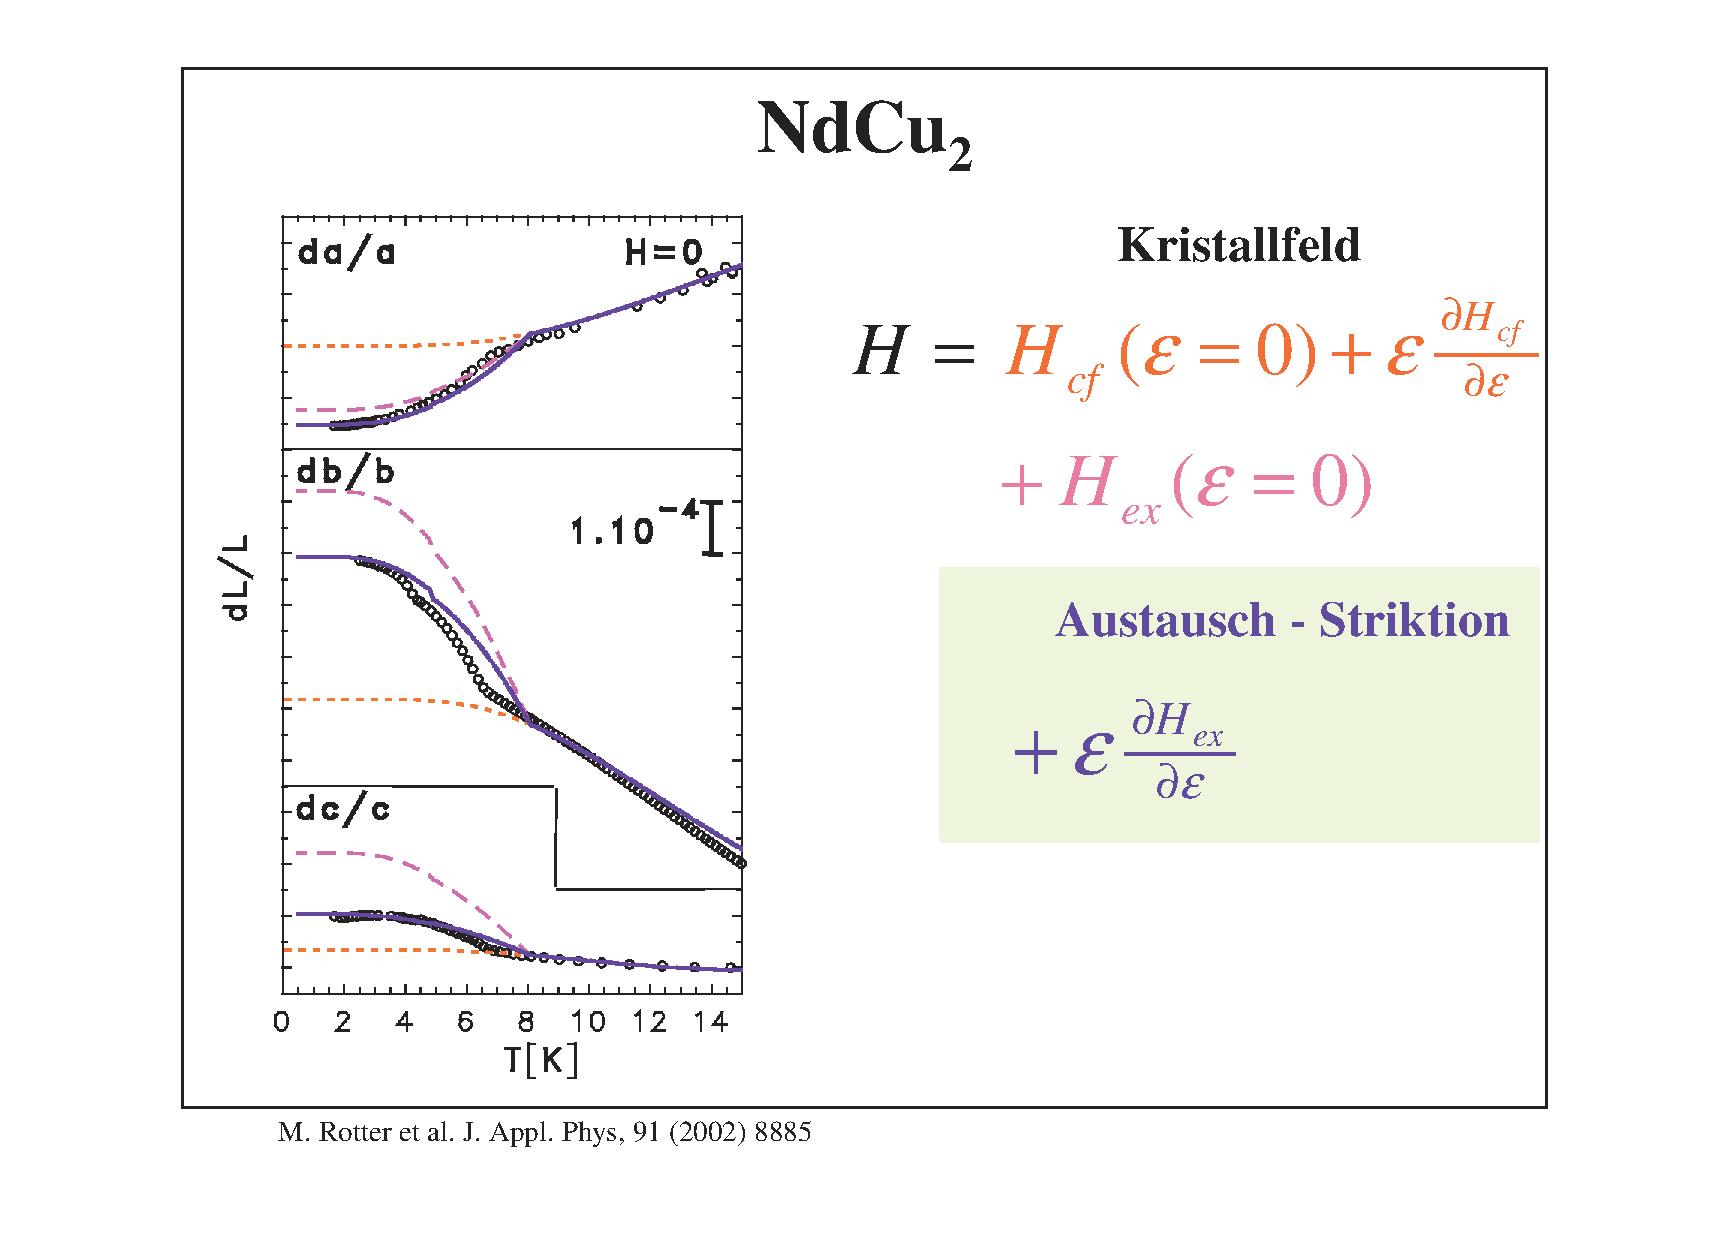
\includegraphics[angle=0, width=0.8\textwidth]{figsrc/magnetostriction_ndcu2.eps}
\end{center}
\caption{Calculated spontaneous magnetostriction of NdCu$_2$.}
\label{magnetostrictiongraphic}
\end{figure}

\begin{description}
\item [\prg mcphas.qvc]    the set of test q-vectors used for calculation of free energy.
                           Components of these q vectors refer to the reciprocal lattice $\vec a^*,\vec b^*,\vec c^*$.
\item [\prg mcphas.phs]    spin-configuration table of different types of spin-configurations. 
                            Note, in case of non-orthogonal axes the convention in these tables 
                            is $mb||\vec b$, $mc||(\vec a \times \vec b)$ and $ma$ perpendicular to $mb$ and $mc$.

                           {\em Note}: 
                           there is no natural criteria for deciding, if one spin-configuration is
			   different from another one. Therefore the list of ''different''
			   spin-configurations is dependent on the meaning of ''different''.
			   
			   The program {\prg McPhase} decides whether a spin-configuration is
			   different from another by a simple criteria, namely by the
			   angle between the spins. Comparing two spin configurations it calculates
			   the angle between corresponding spins and if for one spin the
			   angle is not small, the configuration is treated as a different
			   configuration. Therefore for example a ferromagnet with moments
			   in $a$ has a different spin configuration than a ferromagnet with
			   moments in $b$ direction. 
\item [\prg mcphas.sps]    $T-H$ dependence of spin-configuration. The spin configurations stored in this
                           file may be displayed using the program {\prg spins\index{spins}}, an example is given
			   in figure~\ref{spingraphic}.
                            Note, in case of non-orthogonal axes the convention for applied field $Ha, Hb,Hc$ and
                            also for the moment components $ma, mb, mc$ in these tables 
                            is $mb||\vec b$, $mc||(\vec a \times \vec b)$ and $ma$ perpendicular to $mb$ and $mc$.

\item [\prg mcphas.mf]     $T-H$ dependence of exchange field configuration, stored as $g_J \mu_B H_{xc}(i)$(unit is in meV)
                            for i=1,2,...,number of spins in magnetic unit cell.
                            Note, in case of non-orthogonal axes the convention for applied field $Ha, Hb,Hc$ and
                            also for the mean field components in these tables 
                            is $Hb||\vec b$, $Hc||(\vec a \times \vec b)$ and $Ha$ perpendicular to $Hb$ and $Hc$.
\item [\prg mcphas.fum]    free energy, magnetic energy (the derivative with respect to temperature gives the specific %%@
heat),
                           magnetisation data and (if cfield is used with higher order interactions)
                           expectation values of the Stevens Operators $<O_l^m>$ . As an example for the information
			   contained in this file the calculated magnetisation and magnetostriction of NdCu$_2$ is shown in
			   figures~\ref{magnetization} and ~\ref{magnetizationgraphic}.
                            Note, in case of non-orthogonal axes the convention for applied field $Ha, Hb,Hc$ and
                            also for the magnetisation components $ma,mb,mc$ in these tables 
                            is $Hb||\vec b$, $Hc||(\vec a \times \vec b)$ and $Ha$ perpendicular to $Hb$ and $Hc$.

\item [\prg mcphas1.j1 .j1 .j2 ...] 
               spin-spin correlation functions for sub-lattice 1 neighbour 1 2 ...
	       (linear combination is proportional to magnetostriction)
	       The spin-spin correlation functions for neighbour $k$ are defined by
	       the following sum of dyadic products:

	       \begin{equation}
	        \frac{1}{n}\sum_{s=1}^n <{\mbf J}^s> \times  <{\mbf J}^{s+k}>
	       \end{equation}
	       with $n$ being the number of moments in the magnetic unit cell.
	       Single ion and two-ion magnetostriction can be calculated using the $<O_l^m>$ and the
	       spin-spin correlation functions. As an example the magnetostriction analysis of
	       NdCu$_2$ is shown in figure~\ref{magnetostrictiongraphic}. For details 
             please refer to~\cite{rotter02-8885}.
                            Note, in case of non-orthogonal axes the convention for applied field $Ha, Hb,Hc$ and
                            also for the moment components in these tables 
                            is $Hb||\vec b$, $Hc||(\vec a \times \vec b)$ and $Ha$ perpendicular to $Hb$ and $Hc$.
\item [\prg mcphas.xyt]    phase diagram as x,y,T, H, phase-number j according to spin-configuration table
               given in mcphas.phs, a periodicity key, nettomoments <J>.
 Figure~\ref{phasediagramgraphic}
	       shows the phase diagram of NdCu$_2$ for magnetic fields parallel to the orthorhombic $b$-direction.
                            Note, in case of non-orthogonal axes the convention for applied field $Ha, Hb,Hc$ 
                             in these tables 
                            is $Hb||\vec b$, $Hc||(\vec a \times \vec b)$ and $Ha$ perpendicular to $Hb$ and $Hc$.
\item [\prg mcphas.hkl]    calculated (unpolarised) neutron diffraction data (the calculated magnetic intensities
    correspond to the magnetic structure + Polarisation factor. The
    Lorentz-factor , magnetic form factor and  instrumental corrections are not calculated.)
 As an example figure~\ref{neutintgraphic}
    shows the calculated temperature dependence of magnetic amplitudes for NdCu$_2$.
                           $h,k,l$ refer to the reciprocal lattice $\vec a^*,\vec b^*,\vec c^*$.
                            Note, in case of non-orthogonal axes the convention for applied field $Ha, Hb,Hc$ 
                             in these tables 
                            is $Hb||\vec b$, $Hc||(\vec a \times \vec b)$ and $Ha$ perpendicular to $Hb$ and $Hc$.
    
\item [\prg mcphasa.hkl]    Fourier Transform of the $a$-component of the magnetic Moments.
                           $h,k,l$ refer to the reciprocal lattice $\vec a^*,\vec b^*,\vec c^*$.
                            Note, in case of non-orthogonal axes the convention for applied field $Ha, Hb,Hc$ and
                            the magnetic moment component in these tables 
                            is $Hb||\vec b$, $Hc||(\vec a \times \vec b)$ and $Ha$ perpendicular to $Hb$ and $Hc$.
\item [\prg mcphasb.hkl]    Fourier Transform of the $b$-component of the magnetic Moments.
                           $h,k,l$ refer to the reciprocal lattice $\vec a^*,\vec b^*,\vec c^*$.
                            Note, in case of non-orthogonal axes the convention for applied field $Ha, Hb,Hc$ and
                            the magnetic moment component in these tables 
                            is $Hb||\vec b$, $Hc||(\vec a \times \vec b)$ and $Ha$ perpendicular to $Hb$ and $Hc$.
\item [\prg mcphasc.hkl]    Fourier Transform of the $c$-component of the magnetic Moments.
                           $h,k,l$ refer to the reciprocal lattice $\vec a^*,\vec b^*,\vec c^*$.
                            Note, in case of non-orthogonal axes the convention for applied field $Ha, Hb,Hc$ and
                            the magnetic moment component in these tables 
                            is $Hb||\vec b$, $Hc||(\vec a \times \vec b)$ and $Ha$ perpendicular to $Hb$ and $Hc$.
\end{description} 

\vspace{1cm}
{\em Exercises:}
\begin{itemize}
\item Look at the output files of {\prg McPhase}  in the directory
{\prg examples/ndcu2b\_new/results}.  At which magnetic field
the ferromagnetically aligned state is achieved (at $T=$2~K)?
\item
What is the propagation vector in the different antiferromagnetic phases at $T=$2~K ?
\end{itemize}



\clearpage

\section{{\prg mcdiff}\index{mcdiff} - calculate and fit a magnetic Neutron or Resonant Xray %%@
Scattering}\label{mcdiff}

In order to calculate neutron diffraction and resonant magnetic Xray scattering
at a specified temperature and magnetic field you can use the module {\prg mcdiff\index{mcdiff}}.
An input file {\prg mcdiff.in } for this program can be easily created from
the output file {\prg mcphas.sps} by the program {\prg setup\_mcdiff\_in\index{setup\_mcdiff\_in}}
(in {\prg mcdiff.in } structural data of non magnetic atoms and wavelength
                        and maximal angle have to be edited).
\footnote{Alternatively, one may make use of the program {\prg spins\index{spins}}.} 
{\prg mcdiff\index{mcdiff}} then calculates neutron reflection and intensity list.

Here follows an example input file (see examples/ndcu2b\_new/mcdiff\index{mcdiff}.in):

{\footnotesize
\begin{verbatim}
# this file is the input file read by program mcdiff version 3.0 Tue Jun 23 12:51:43 2009
#<!--mcdiff.mcdiff.in>
#***************************************************************
#      mcdiff is a program for the calculation of elastic
#   neutron diffraction and resonant magnetic Xray scattering 
#  reference: M. Rotter and A. Boothroyd PRB 79 (2009) 140405R
#*************************************************************** 
# this input file contains 4 sections corresponding to different
# groups of parameters
#
# - all lines have to start with a # sign with the  exception of 
#   the lines containing atomic positional parameters
# - the other parameters have to be defined in the corresponding 
#   section by statements such as parameter=value
# - the sequence of the parameters within a section is arbitrary
# 
#
# %SECTION 1%  OVERALL PARAMETERS
#
#! lambda   = 0.9  wavelength (A)
#
#! thetamax = 19   maximum bragg angle (deg)
#
#! ovalltemp= 0.3  overall temperature factor (A^2) 
#           ...I ~ EXP(-2 * ovalltemp * sintheta^2 / lambda^2) 
#                  relation to other notations:
#                  ovalltemp = Biso = 8 pi^2 Uiso^2
#
#! lorentz=1  type of lorentzfactor to be used
#            0.....no lorentzfactor 
#            1.....neutron powder flat sample
#            2.....neutron powder cylindrical sample
#            3.....neutron single crystal
#            4.....neutron TOF powder cyl. sample - d-pattern log scaled
#            5.....neutron TOF powder cyl. sample - d-pattern normal scaled
#
#! out10=1    type of desired output in column 10 and 11 of mcdiff.out
#! out11=0    (optional) default is NSF in column 10 and LF in column 11
#            0....LF
#            1....|NSF|[b]
#            2....Re(NSF)[b]
#            3....Im(NSF)[b]
#            4....|MSF|
#            5....|MSF.P|
#            6....Re(MSF.P)
#            7....Im(MSF.P)
#            8....|MSFdip|
#            9....|MSFdip.P|
#            10....Re(MSFdip.P)
#            11....Im(MSFdip.P)
#            12....angl(Q,P)[°]
#            13....i(MSF x MSF*).P
#            14.... I+
#            15.... I-
#            16....I+/I-
#
#           In the above the intensities I+ and I- are the spinflip and nonspineflip intensities
#           in a polarised neutron experiment:
#            I+-=LF exp(-OTF Q^2/8pi^2) 
#                    [ |NSF/NB|^2 + 3.65/4pi (|MSF/NB|^2-i(MSF x MSF*).P) 
#                        +-  sqrt(3.65/4pi)/NB^2 (NSF (MSF*.P) + NSF* (MSF.P)]
#
#
#             For some of the above options we need the Projection (=polarization of neutron beam) vector
#! Pa=  1.0000   Components of Projection Vector P=(Pa * a + Pb * b + Pc *c)/Norm(Pa * a + Pb * b + Pc *c)
#! Pb=  0.0000
#! Pc=  0.0000
#
#
# %SECTION 2% LIST OF NONMAGNETIC ATOMS IN CRYSTALLOGRAPHIC UNIT CELL
#
#
#! nat=1      number of nonmagnetic atoms in primitive crystalographic unit cell
#
# it follows a list of nat lines with nonmagnetic atoms
# ... notes: - if an occupancy other than 1.0 is needed, just reduce 
#              the scattering length linear accordingly
#            - da db and dc are not used by the program (unless you enter a line #! use_dadbdc=1), 
#              dr1,dr2 and dr3 refer to the primitive lattice given below
#            - Debye Waller Factor notation: sqr(Intensity) ~ structure factor ~ 
#              ~sum_n ()n exp(-2 DWFn sin^2(theta) / lambda^2)=EXP (-Wn),  
#              relation to other notations: 2*DWF = B = 8 pi^2 <u^2>, units DWF (A^2)
#
# Real Imag[scattering length(10^-12cm)]   da(a)    db(b)    dc(c)    dr1(r1)  dr2(r2)  dr3(r3)  DWF(A^2)
   0.77200   0.00000                        0.50000  0.50000  0.50000  0.50000  0.50000  0.50000  0.00000
#
#
# %SECTION 3% DESCRIPTION OF THE LATTICE
#
#
# Note: what follows here may directly be taken from the output of program spins 
#       (file spins.out) or charges (file charges.out)
# -----------------------------------------------------------------------------
#
# lattice constants (A) and angles 
#! a=4.3843 b=4.3843 c=2.4194 alpha=  90 beta=  90 gamma=  90
#
# primitive lattice vectors 
#! r1a= 1.000000 r2a= 0.000000 r3a= 0.000000
#! r1b= 0.000000 r2b= 1.000000 r3b= 0.000000   primitive lattice vectors (a)(b)(c)
#! r1c= 0.000000 r2c= 0.000000 r3c= 1.000000
#
#
#
# %SECTION 4% DESCRIPTION OF MAGNETIC UNIT CELL AND LIST OF MAGNETIC ATOMS
#
#
# here follows the description of the magnetic unit cell with respect
# to the primitive crystallographic unit cell:
# 'nr1', 'nr2', 'nr3' ...the crystallographic unit cell has to be taken 
#                        nr1 nr2 and nr3 times along r1 r2 and r3,
#                        respectively to get magnetic unit cell
# 'nat' denotes the number of magnetic atoms in magnetic unit cell
#
# Temperature,    Magnetic Field: Magnetic Unit Cell
#! T=2 K Ha=0 T Hb= 0 T Hc= 0 T: nr1=1 nr2=1 nr3=2 nat=2 
#
#
# It follows a list of nat lines with to describe the magnetic moment configuration
# Notes:
# 'atom-filename' means the single ion property filename of this magnetic atom:
#                 -it must contain the Formfactor Coefficients (e.g. see international tables)
#                                      Lande factor
#                                      Neutron Scattering Length (10^-12 cm) 
#                 -it may contain a    Debey Waller Factor
# 'da' 'db' and 'dc' are not used by the program (unless you enter a line #! use_dadbdc=1), 
# 'dr1','dr2' and 'dr3' refer to the primitive lattice given below
# 'Ma','Mb','Mc' denote the magnetic moment components in Bohr magnetons along the axes a b and c
#                in case of non orthogonal lattices instead of Ma Mb Mc the components Mi Mj Mk
#                have to be given, which refer to an right handed orthogonal coordinate system 
#                defined by j||b, k||(a x b) and i normal to k and j
# '<Ja>' '<Jb>' '<Jc>' (optional) denote the momentum components 
# 'gjmbHeffa' 'gjmbHeffb' 'gjmbHeffc' (optional line, used to go beyond dipole approx for formfactor)
#                                     denote the corresponding meanfields multiplied by 
#                                     Lande factor and Bohr magneton 
#
#{atom-file} da[a]  db[b]    dc[c]     dr1[r1]  dr2[r2]  dr3[r3]   <Ma>     <Mb>     <Mc> [mb] <Ja>     <Jb>     %%@
<Jc> ...
#{corresponding effective fields gjmbHeff [meV]- if passed to mcdiff only these are used for caculation (not %%@
the magnetic moments)}
{mcphas.cf1}  0.00000  0.00000  0.00000   0.00000  0.00000  0.00000   +0.00000 +0.00000 -2.13030  +0.00000 %%@
+0.00000 -2.48540
{mcphas.cf1}  0.00000  0.00000  1.00000   0.00000  0.00000  1.00000   +0.00000 +0.00000 +2.13030  +0.00000 %%@
+0.00000 +2.48540

\end{verbatim}
}

After issuing the command {\prg mcdiff\index{mcdiff}} 
the program calculates the following output file {\prg results/mcdiff\index{mcdiff}.out}:

{\footnotesize
\begin{verbatim}
#{output file of program mcdiff ./results/mcdiff.out input file: mcdiff.in mcdiff version 3.0 Tue Jun 23 %%@
12:51:43 2009
#!<--mcdiff.mcdiff.out-->
#***********************************************************************
#*
#* mcdiff - program to calculate neutron and magnetic xray diffraction
#*
#* reference: M. Rotter and A. Boothroyd PRB 79 (2009) 140405R
#***********************************************************************
#! unit cell: a= 4.3843 A  b= 4.3843 A c= 2.4194 A  alpha=90  beta=90 gamma=90
#                   /  0.000 A \     /  0.000 A \     /  4.839 A \ 
#                r1=|  4.384 A |  r2=|  0.000 A |  r3=| -0.000 A |
#                   \ -0.000 A /     \  4.384 A /     \ -0.000 A /
#! Wavelength=0.9 A   number of atoms: 4
#! T= 2 K Ha= 0 T Hb= 0 T Hc= 0 T
#! Overall temperature factor B=0.3 A^2: Intensity is proportional to exp(-2*B*(sin(theta)/lambda)^2)
# Lorentz Factor: 1 / sin^2(2theta)   neutron powder flat sample
#
# Lorentz Factor not considered for resonant magnetic xray scattering - F1 and F2 transition intensities %%@
calculated
# according to fRMXS as given in equation (2) of Longfield et al. PRB 66 054417 (2002) and maximized with %%@
respect to azimuth.
#
# List of atomic positions dr1 dr2 dr3, moments m scattering lengths sl,
# Debye Waller factor (sqr(Intensity)~|NSF| ~sum_i ()i exp(-2 DWFi sin^2(theta) / lambda^2)=EXP (-Wi),
# units DWF [A^2], relation to other notations 2*DWF=B=8 pi^2 <u^2>)
#  and  Lande factors total angular momentum J (=0 if dipole approximation is used) <j0> and <j2> formfactor
# coefficients
#  dr1[r1]dr2[r2]dr3[r3]ma[MuB]mb[MuB]mc[MuB]sl[10^-12cm]  DWF[A^2] gJ     <j0>:A a      B      b      C      %%@
c      D      <j2>A  a      B      b      C      c      D
#  0.000  0.000  0.000  0.000  0.000 -2.130  0.484+0.000i  0.000  0.857 F(Q)=j0-(1-2/gJ)j2 formfactor for %%@
rare earth/transition metals with gJ=2 0.295 17.685  0.292  6.733  0.431  5.383 -0.019  0.981 18.063  1.841  %%@
7.769  0.991  2.845  0.012 
#  0.000  0.000  0.500  0.000  0.000  2.130  0.484+0.000i  0.000  0.857 F(Q)=j0-(1-2/gJ)j2 formfactor for %%@
rare earth/transition metals with gJ=2 0.295 17.685  0.292  6.733  0.431  5.383 -0.019  0.981 18.063  1.841  %%@
7.769  0.991  2.845  0.012 
#  0.500  0.500  0.250  0.000  0.000  0.000  0.772+0.000i  0.000  0.000  1.000  0.000  0.000  0.000  0.000  %%@
0.000  0.000  0.000  0.000  0.000  0.000  0.000  0.000  0.000 
#  0.500  0.500  0.750  0.000  0.000  0.000  0.772+0.000i  0.000  0.000  1.000  0.000  0.000  0.000  0.000  %%@
0.000  0.000  0.000  0.000  0.000  0.000  0.000  0.000  0.000 
#}
#{h     k      l      d[A]    |Q|[1/A] 2theta  Inuc(2t) Imag(2t) Itot(2t) |NSF|     LF   Imag_dip(2t) %%@
F1:max-Isigpi azim Ipisig azim Ipipig azim F2:max-Isigpi azim Ipisig azim Ipipig azim  |^ma_q| |^mb_q| %%@
|^mc_q| |^ma^2_q||^mb^2_q||^mc^2_q||(^ma*^mb)_q||(^ma*^mc)_q||(^mb*^mc)_q|}
 0.000  0.000  0.500  4.8388  1.2985  10.672   0.0000   0.0000   0.0000   0.0000  29.1583   0.0000        %%@
0.010111 270 0.010111  90 0.000000   0   0.000000 360 0.000000 180 0.000000  90    0.0000   0.0000   1.0652   %%@
0.0000   0.0000   0.0000   0.0000   0.0000   0.0000
 0.000  0.000 -0.500  4.8388  1.2985  10.672   0.0000   0.0000   0.0000   0.0000  29.1583   0.0000        %%@
0.010111  90 0.010111 270 0.000000 360   0.000000 180 0.000000 360 0.000000  90    0.0000   0.0000   1.0652   %%@
0.0000   0.0000   0.0000   0.0000   0.0000   0.0000
 1.000  0.000  0.000  4.3843  1.4331  11.782   0.4935   0.0000   0.4935   0.5760  23.9836   0.0000        %%@
0.000000   0 0.000000   0 0.000000   0   0.013544 314 0.013544 314 0.000571 270    0.0000   0.0000   0.0000   %%@
0.0000   0.0000   2.2691   0.0000   0.0000   0.0000
-1.000  0.000 -0.000  4.3843  1.4331  11.782   0.4935   0.0000   0.4935   0.5760  23.9836   0.0000        %%@
0.000000   0 0.000000   0 0.000000   0   0.013544 314 0.013544 314 0.000571 270    0.0000   0.0000   0.0000   %%@
0.0000   0.0000   2.2691   0.0000   0.0000   0.0000
 0.000  1.000 -0.000  4.3843  1.4331  11.782   0.4935   0.0000   0.4935   0.5760  23.9836   0.0000        %%@
0.000000   0 0.000000   0 0.000000   0   0.013544 314 0.013544 314 0.000571 270    0.0000   0.0000   0.0000   %%@
0.0000   0.0000   2.2691   0.0000   0.0000   0.0000
-0.000 -1.000  0.000  4.3843  1.4331  11.782   0.4935   0.0000   0.4935   0.5760  23.9836   0.0000        %%@
0.000000   0 0.000000   0 0.000000   0   0.013544 314 0.013544 314 0.000571 270    0.0000   0.0000   0.0000   %%@
0.0000   0.0000   2.2691   0.0000   0.0000   0.0000
 1.000  0.000  0.500  3.2490  1.9339  15.923   0.0000   0.4821   0.4821   0.0000  13.2870   0.4821        %%@
0.775763   0 0.775763 180 0.046891  90   0.000000  98 0.000000 278 0.000000   0    0.0000   0.0000   1.0652   %%@
0.0000   0.0000   0.0000   0.0000   0.0000   0.0000
 1.000  0.000 -0.500  3.2490  1.9339  15.923   0.0000   0.4821   0.4821   0.0000  13.2870   0.4821        %%@
0.775763 360 0.775763 180 0.046891 270   0.000000 262 0.000000  82 0.000000 360    0.0000   0.0000   1.0652   %%@
0.0000   0.0000   0.0000   0.0000   0.0000   0.0000
etc ....
-----------------------------------------------------------------------
\end{verbatim}
}

This reflection list contains the Miller indices, the d-spacing, the scattering vector,
the scattering angle 2$\Theta$, nuclear and magnetic neutron scattering intensities
and the corresponding structure-, Lorentzfactor. Moreover it contains the
intensities for the different scattering channels of resonant magnetic x-ray scattering,
the intensity is shown together with the azimuth value where it is maximum. In addition,
the absolute value of the Fourier transform of the magnetic moment components in the different
crystal directions and of some products of the moment components is given.

\subsection{How to generate and view a powder diffraction profile}


.. such a reflection list can be easily transformed into a diffraction pattern
by convolution with the resolution function of a neutron diffractometer.

\begin{itemize}
\item
Simple resolution functions can be easily generated with the help of the programs
{\prg gauss\index{gauss}} and {\prg lorentz\index{lorentz}}. Any other numerical
resolution function, e.g. from a measurement or simulation can be used.
\item
Use program  {\prg convolute\index{convolute}} for doing the convolution. 
Here is an example command: 
{\prg convolute\index{convolute} 6 8  results/mcdiff\index{mcdiff}.out
1 2 resultshb/resolution.dat}
... this gives magnetic pattern such as shown in fig.~\ref{elnpattern}
\item Usually the convolution needs to be done to compare to experimental
data and needs only to be evaluated at the experimental data points, for
example the measured scattering angle values $2\Theta$. This can be 
done by adding a data file to the command,
{\prg convolute\index{convolute} 6 8  results/mcdiff\index{mcdiff}.out
1 2 resultshb/resolution.dat 1 2 datafile.dat}. In our example the
data file contains the experimental data in columns 1 (angle) and columns 2 (Intensity).
\item If needed the resolution function can be stretched using stretching
values given in a separate column of the data file - the command is then
{\prg convolute\index{convolute} 6 8  results/mcdiff\index{mcdiff}.out
1 2 resultshb/resolution.dat 1 2 datafile.dat 13} (in this example the stretching
factor is taken from column 13 of the datafile.
\item Generating of the stretching factor: the stretching factor
may be generated by program {\prg uvw2fwhm\index{uvw2fwhm}} from
the scattering angle values and the parameters U,V and W (as in {\prg FullProf\index{FullProf}}.

\end{itemize}

\begin{figure}[ht]
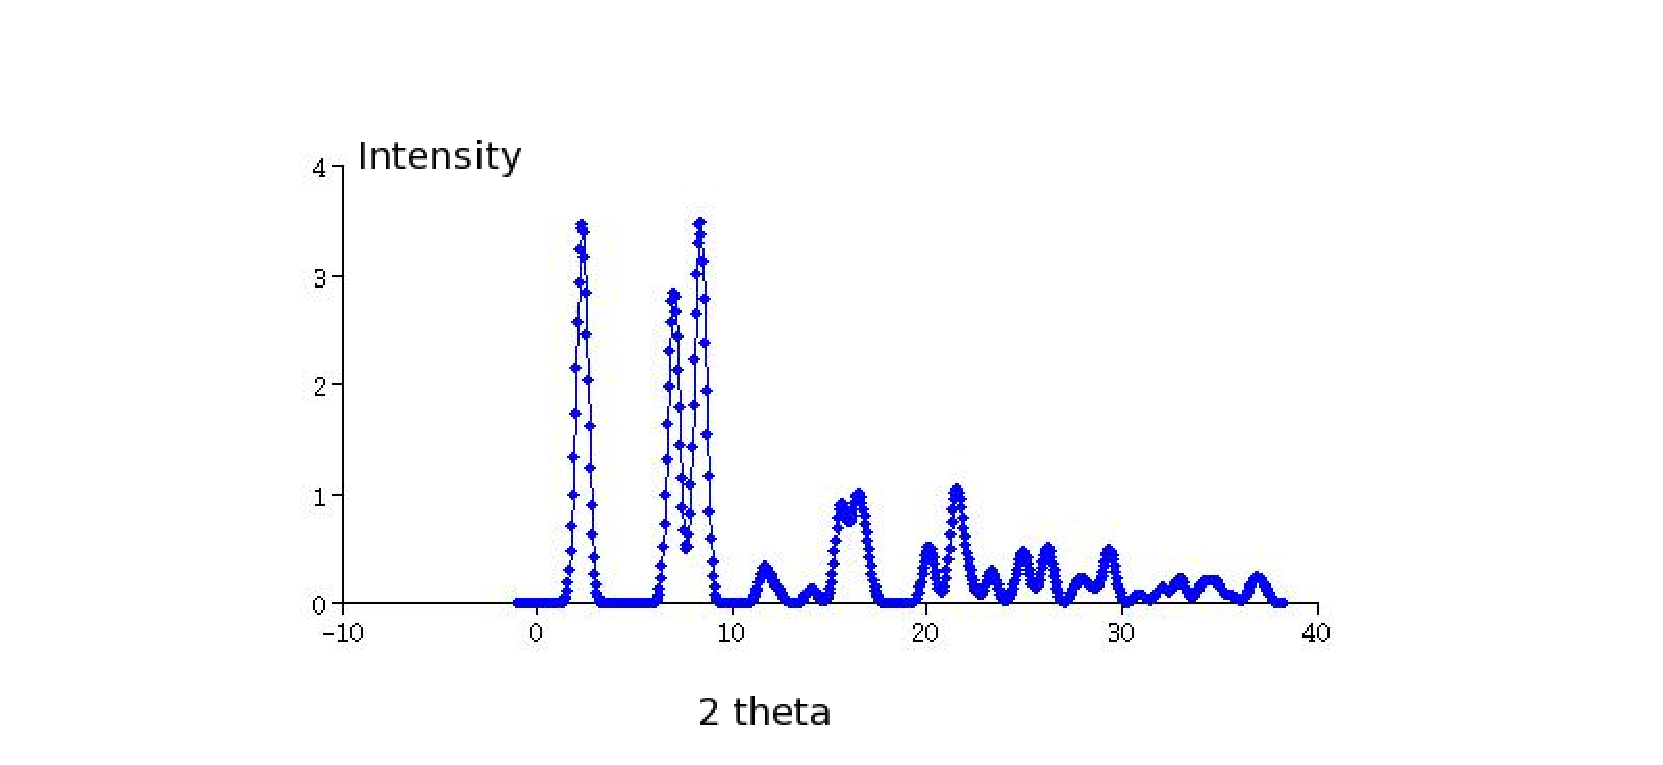
\includegraphics[angle=0,width=1.1\textwidth]{./figsrc/patternAF1.eps}
\caption{\label{elnpattern}
Calculated magnetic neutron powder diffraction pattern
of NdCu$_2$~\cite{gratz91-9297} at T=2~K.
[plot created by program {\prg mcdiff\index{mcdiff}+convolute\index{convolute}+display}]}
\end{figure}

\subsection{How to calculate only specific reflections, azimuth dependence and fitting of neutron %%@
intensities}

For the fit of experimental intensities it is often desirable to save computation
time by calculating the intensity only for a specified set of reflections and 
compare it to experimental data. Such list should have the following format

\begin{verbatim}
#{h     k     l }
0.500 0.500 0.500 
0.500 0.500 1.500 
0.500 0.500 2.500 
\end{verbatim}

Lets assume such a list is stored  as file {\prg hkllist.dat}.
Then {\prg mcdiff\index{mcdiff}} can be started as: {\prg mcdiff\index{mcdiff} hkllist.dat}.
The output file will then contain the azimuth dependence of the magnetic intensity.

Alternatively, experimental intensities can be entered in the list, for example as

\begin{verbatim}
#{h  k   l       Iexp err}
0.500 0.500 0.500 115 4
0.500 0.500 1.500 84  3
0.500 0.500 2.500 50  1
0.500 0.500 3.500 29  1
0.500 0.500 4.500 22  2
0.500 0.500 5.500 15  1
0.500 0.500 6.500 12  1
#
1.500 1.500 0.500 -1
1.500 -1.50 0.500 -1
-1.50 1.500 0.500 77  8
1.500 1.500 1.500 65  7
1.500 1.500 2.500 59  5
1.500 1.500 3.500 51  5
\end{verbatim}

In this case the calculated neutron intensities are compared to
the experimental intensities and the Rp value $R_{\rm p}=100
\frac{\sum_{hkl} |I_{calc}(hkl)-I_{exp}(hkl)|}{\sum_{hkl}|I_{\rm
exp}(hkl)|}$. and $\chi^2=\sum_{hkl}\frac{ (I_{calc}(hkl)-I_{exp}(hkl))^2}{n(\Delta I_{\rm
experror}(hkl))^2}$
is calculated (here $n$ denotes the number of experimental reflections). 

Note, a negative experimental intensity in this
list means, that the intensity of that reflection has to
be added to the intensity of the next reflection in the list 
and the sum should be compared to an experimental intensity.
In this way domains or overlapping reflections can be treated. 
The program will always calculate the intensity for each reflection
seperately, if you wish to calculate the sum of intensities, which
are compared to the experimental intensity, use program {\prg sum\_mcdiff\_out}\index{sum\_mcdiff\_out}.

\subsection{Formalism I - Resonant Magnetic Xray Scattering Intensity}

The resonant magnetic scattering intensity is calculated as outlined for example in~\cite{longfield02-054417}
for the magnetic electric dipole scattering according to the squared absolute value of the scattering
amplitude given for the ion $n$ in the lattice as

\begin{eqnarray}
&&f_{nE1}^{RXMS}=   \\
&&=\left (
\begin{array}{cc}
\sigma \rightarrow \sigma & \pi \rightarrow \sigma \\
\sigma \rightarrow \pi & \pi \rightarrow \pi 
\end{array}
 \right) = F^{(0)}
\left ( \begin{array}{cc}
1 & 0 \\
0 & \cos2\Theta 
\end{array} \right )
-iF^{(1)}  \nonumber \\
&&\times 
\left ( \begin{array}{cc}
0 & z_1 \cos \Theta + z_3 \sin \Theta \\
z_3 \sin \Theta - z_1 \cos \Theta & -z_2 \sin 2\Theta  
\end{array} \right ) + F^{(2)}\nonumber \\
&&\times 
\left ( \begin{array}{cc}
z_2^2 & -z_2(z_1 \sin \Theta - z_3 \cos \Theta) \\
+z_2(z_1 \sin \Theta + z_3 \cos \Theta) & -\cos^2 \Theta (z_1^2 \tan^2 \Theta + z_3^2)
\end{array} \right ) \nonumber \\
\end{eqnarray} 

Here, dropping the site index $n$, $\Theta$ is the Bragg scattering angle and
$z_1, z_2$ and $z_3$ aree components of the magnetization vector with respect
to the coordinate system $[\mbf u_1,\mbf u_2,\mbf u_3]$. The scattering plane, defined by the
direction of the incident and final wave vectors  $\mbf k$ and $\mbf k'$, contains $\mbf u_1$ lying
perpendicular and in the sense of $\mbf k$ and $\mbf u_3$ antiparallel to the scattering
vector $\mbf Q=\mbf k'-\mbf k$. The scattering channels for $F^{(1)}$ and $F^(2)$ terms are considered
separately and no interference is considered. 

To determine the azimuthal dependence the $z_i$ are expanded in terms of the components
$\mu_a,\mu_b$ and $\mu_c$ of the magnetic moment along the orthogonal crystallographic
unit cell vectors $\mbf a$,$\mbf b$ and $\mbf c$:

\begin{eqnarray}
z_1&=&\mu_a \sin \alpha_1 \cos(\Psi+\delta_1)+\mu_b \sin \alpha_2 \cos(\Psi +\delta_2) \nonumber \\
&& +\mu_c \sin \alpha_3 \cos (\Psi +\delta_3), \nonumber \\
z_2 & = & \mu_a \sin \alpha_1 \sin (\Psi +\delta_1)+\mu_b \sin \alpha_2 \sin (\Psi+\delta_2) \nonumber \\
& & +\mu_c \sin \alpha_3 \sin (\Psi +\delta_3) \nonumber \\
z_3 & = & \mu_a \cos \alpha_1 + \mu_b \cos \alpha_2 + \mu_c \cos \alpha_3 
\end{eqnarray}
 
with angles $\alpha_i=\angle(\mbf a_i \cdot \mbf u_3)_{\Psi=0}$ and $\delta_i=\angle(\mbf a_i^{\perp}\cdot %%@
\mbf u_1)_{\Psi=0}$, where $\mbf a_{1,2,3}=\mbf a,\mbf b,\mbf c$ and $\mbf a_i^{\perp}$ is the projection of
$\mbf a_i$ onto the plane perpendicular to $\mbf Q$. In the chosen experimental geometry
$\Psi=0$ when $\mbf a$ points to the x-ray source.


\subsection{Formalism II - Neutron Cross section}

{\prg mcdiff\index{mcdiff}} uses the standard formalism to calculate the elastic neutron scattering
cross section, which can be obtained from the elastic part of the double differential
cross section:

\begin{equation}\label{dsdode}
\frac{d^2\sigma}{d\Omega dE'}=N\frac{k'}{k}\left( \frac{\hbar \gamma e^2}{m_e c^2}  \right)^2
%\sum_{\mbf Q} \delta_{\vec\kappa,\mbf Q}
\sum_{\alpha\beta}(\delta_{\alpha\beta}-\hat \mbf Q_{\alpha} \hat \mbf Q_{\beta}) 
S^{\alpha \beta}_{\rm mag}(\mbf Q,\omega)+
N\frac{k'}{k}S_{\rm nuc}(\mbf Q,\omega)
\end{equation}

In equation (\ref{dsdode}) $\frac{d^2\sigma}{d\Omega dE'}$ denotes the double differential
cross section, $N$ the number of atoms, $k$ and $k'$ the wave vectors of the incoming and
scattered neutron, respectively. $\gamma=\frac{g_n}{2\hbar}$ 
is the gyromagnetic ratio of the neutron and $e^2/m_ec^2=2.82$~fm is the classical
electron radius, $\mbf Q=\mbf k-\mbf k'$ the scattering vector, 
$\hbar \omega=E-E'=\frac{(\hbar\mbf k)^2}{2m_n}-\frac{(\hbar\mbf k')^2}{2m_n}$
the energy transfer and the $S$ are the nuclear and magnetic Van Hove scattering functions.
Both are a sum of elastic and inelastic contributions:

\begin{eqnarray}
S_{\rm nuc}&=&S_{\rm nuc}^{\rm el}+S_{\rm nuc}^{\rm inel} \\
S_{\rm mag}&=&S_{\rm mag}^{\rm el}+S_{\rm mag}^{\rm inel}  
\end{eqnarray}

The nuclear elastic scattering can be split into a coherent and an 
incoherent part:

\begin{equation}
S_{\rm nuc}^{\rm el}=S_{\rm nuc}^{\rm el,inc}+S_{\rm nuc}^{\rm el,coh}
\end{equation}

The nuclear elastic coherent scattering function is given by a product
of lattice factor and nuclear structure factor NSF:

\begin{eqnarray}
S_{\rm nuc}^{\rm el,coh}&=&\delta(\hbar \omega) 
\left ( \frac{(2\pi)^3}{v_0}\sum_{\mbf \tau} \delta(\mbf Q-\mbf \tau) \right )
\frac{1}{N_B} \left ( \sum_{dd'} \bar b_d^* \bar b_{d'} e^{-i\mbf Q(\mbf B_d-\mbf B_{d'})} e^{-W_d-W_{d'}} %%@
\right )\\
&=&\delta(\hbar \omega)
\left ( \frac{(2\pi)^3}{v_0}\sum_{\mbf \tau} \delta(\mbf Q-\mbf \tau) \right )
\frac{1}{N_B}|NSF|^2
\end{eqnarray}

$N_B$ denotes the number of atoms in the basis and the sums run over
all reciprocal lattice vectors $\mbf \tau$ and over all atoms $d=1,\dots,N_B$
in the unit cell (unit cell volume is $v_0$). 
$\bar b_d$, $\mbf B_d$ and $W_d$ are the coherent scattering length, the unit cell
position vector and the Debye Waller factor of the atom $d$ 
($W_d= \langle (\mbf Q.\mbf u_d)^2 \rangle/2=\langle u_{\rm iso}^2 \rangle Q^2/2=B_{\rm iso}Q^2/16\pi^2=
B_{\rm iso} sin^2 \Theta / \lambda^2$), respectively. 

Similar, the magnetic elastic scattering function can be written as a product:

\begin{eqnarray}\label{msf}
\sum_{\alpha\beta}(\delta_{\alpha\beta}-\hat \mbf Q_{\alpha} \hat \mbf Q_{\beta})S_{\rm mag}^{\rm %%@
el,\alpha\beta}&=&\delta(\hbar \omega) 
\left ( \frac{(2\pi)^3}{v_0}\sum_{\mbf \tau} \delta(\mbf Q-\mbf \tau) \right )
\frac{1}{N_B} \left ( \sum_{dd',\alpha\beta}(\delta_{\alpha\beta}-\hat \mbf Q_{\alpha} \hat \mbf Q_{\beta})
{\frac{1}{2\mu_B}F(Q)}_d M_{d\alpha} \right. 
\nonumber \\ 
&&\left.  {\frac{1}{2\mu_B}F(Q)}_{d'} M_{d'\beta}
 e^{-i\mbf Q(\mbf B_d-\mbf B_{d'})} e^{-W_d-W_{d'}} \right )\\
&=&\delta(\hbar \omega)\left ( \frac{(2\pi)^3}{v_0}\sum_{\mbf \tau} \delta(\mbf Q-\mbf \tau) \right )
\frac{1}{N_B} |\vec{\rm MSF}|^2
\end{eqnarray}

with $M_{d\alpha}/\mu_B=g_J\langle J_{d\alpha} \rangle_{T,H}$.
Here $g_J$, $F(Q)$ and $\langle J_{d\alpha} \rangle_{T,H}$ denote the
Land\'e factor, the form factor and the expectation value of the total angular
momentum operator of the atom $d$ in the unit cell, respectively.

Program {\prg mcdiff\index{mcdiff}} calculates the 
scattering angle $2\Theta$ of a reflection 
$\mbf Q=h\mbf a^*+k \mbf b^*+l \mbf c^*$
according to 

\begin{equation}
\sin(\Theta)=\lambda \frac{|\mbf Q|}{4\pi}
\end{equation}

Nuclear elastic coherent and magnetic intensities are calculated
according to:

\begin{equation}
I^{nuc}_{hkl}=|\frac{\rm NSF}{N_B}|^2 \exp(-\frac{{\rm OTF}\times Q^2}{8\pi^2}) \times {\rm LF} 
\end{equation}

\begin{equation}
I^{mag}_{hkl}=\frac{3.65}{4\pi}|\frac{\vec{\rm  MSF}}{N_B}|^2  \exp(-\frac{{\rm OTF}\times Q^2}{8\pi^2}) \times {\rm %%@
LF} 
\end{equation}

\begin{eqnarray}
{\rm OTF}&=& {\rm ... Overall Temperature Factor (}B_{\rm iso}),{\rm  OTF}.Q^2/(8\pi^2) =\langle (\mbf Q.\mbf %%@
u)^2 \rangle = \langle u^2 \rangle Q^2  \\
{\rm LF} &=& {\rm ... Lorentzfactor}  \\
              & =& \sin^{-2}(2\Theta){\rm ... powder flat sample}\\
              & =& \sin^{-1}(2\Theta)\sin^{-1}(\Theta){\rm ... powder cylindrical sample}\\
              & =& \sin^{-1}(2\Theta){\rm ...single crystal sample}\\
             & =& d^3 {\rm ... TOF powder cylindrical sample log scaled d pattern}\\
             & =& d^4 {\rm... TOF powder cylindrical sample linear scaled d pattern}\\
{\rm NSF} &=&{\rm ... nuclear structure factor}\\
                 &=&  \sum_{d} \bar b_d e^{i\mbf Q \mbf B_d} e^{-W_d}\\
\vec{\rm MSF} &=&{\rm ... magnetic structure factor}\\
                &=& \sum_{d}\frac{1}{2\mu_B}F_d(Q) \vec M^{\perp}_{d} e^{i\mbf Q\mbf B_d} e^{-W_d} 
\end{eqnarray}

Mind: no absorption and extinction corrections are calculated.


\subsection{Going beyond the Dipole Approximation for the Neutron Form factor}\label{mcdiff_gobeyond}

Usually the magnetic form factor is calculated by the dipole approximation (see appendix~\ref{ffacts}).
In order to go beyond the dipole approximation (see~\cite{lovesey84-1} chapter 11.6.2,equations 
11.141-11.143, mind: there is a small error in equ 11.141 and 11.142 in this book, see below) for the 
magnetic form factor it is necessary to take into account the expectation values
$\langle j_4(Q) \rangle$ and $\langle j_6(Q) \rangle$ 
(in addition to $\langle j_0(Q) \rangle$ and $\langle j_2(Q) \rangle$). 
Moreover the ground state wave functions, the $Z(K)$-coefficients (see appendix~\ref{zk}
or \cite{lovesey84-1},table 11.1)
and the momentum quantum number for each magnetic ion is required. This
information has to be given in the input file 
in the following format:

{\footnotesize
\begin{verbatim}
...
# %SECTION 4% DESCRIPTION OF MAGNETIC UNIT CELL AND LIST OF MAGNETIC ATOMS
#
#
# here follows the description of the magnetic unit cell with respect
# to the primitive crystallographic unit cell:
# 'nr1', 'nr2', 'nr3' ...the crystallographic unit cell has to be taken 
#                        nr1 nr2 and nr3 times along r1 r2 and r3,
#                        respectively to get magnetic unit cell
# 'nat' denotes the number of magnetic atoms in magnetic unit cell
#
# Temperature,    Magnetic Field: Magnetic Unit Cell
#! T=1.3 K Ha=0 T Hb= 0 T Hc= 0 T: nr1=2 nr2=2 nr3=2 nat=8 
#
#
# It follows a list of nat lines with to describe the magnetic moment configuration
# Notes:
# 'atom-filename' means the single ion property filename of this magnetic atom:
#                 -it must contain the Formfactor Coefficients (e.g. see international tables)
#                                      Lande factor
#                                      Neutron Scattering Length (10^-12 cm) 
#                 -it may contain a    Debey Waller Factor
# 'da' 'db' and 'dc' are not used by the program (unless you enter a line #! use_dadbdc=1), 
# 'dr1','dr2' and 'dr3' refer to the primitive lattice given below
# 'Ma','Mb','Mc' denote the magnetic moment components in Bohr magnetons
# '<Ja>' '<Jb>' '<Jc>' (optional) denote the momentum components 
# 'gjmbHeffa' 'gjmbHeffb' 'gjmbHeffc' (optional line, used to go beyond dipole approx for formfactor)
#                                     denote the corresponding meanfields multiplied by 
#                                     Lande factor and Bohr magneton 
#
#{atom-file} da[a]  db[b]    dc[c]     dr1[r1]  dr2[r2]  dr3[r3]   <Ma>     <Mb>     <Mc> [mb] <Ja>     <Jb>     %%@
<Jc> ...
#{corresponding effective fields gjmbHeff [meV]- if passed to mcdiff only these are used for caculation (not %%@
the magnetic moments)}
{Ce3p.sipf} 0.00000  0.00000  0.00000   0.00000  0.00000  0.00000   +0.69590 +0.69620 +0.00000  
                  corresponding effective fields gjmbHeff [meV]--> +0.58640 +0.58660 +0.00000
{Ce3p.sipf} 0.50000  0.50000  0.50000   0.00000  0.00000  1.00000   -0.69590 -0.69620 +0.00000  
                  corresponding effective fields gjmbHeff [meV]--> -0.58640 -0.58660 +0.00000
{Ce3p.sipf} 0.00000  1.00000  0.00000   0.00000  1.00000  0.00000   -0.69590 -0.69620 +0.00000  
                  corresponding effective fields gjmbHeff [meV]--> -0.58640 -0.58660 +0.00000
{Ce3p.sipf} 0.50000  1.50000  0.50000   0.00000  1.00000  1.00000   +0.69590 +0.69620 +0.00000  
                  corresponding effective fields gjmbHeff [meV]--> +0.58640 +0.58660 +0.00000
{Ce3p.sipf} 1.00000  0.00000  0.00000   1.00000  0.00000  0.00000   -0.69590 -0.69620 +0.00000  
                  corresponding effective fields gjmbHeff [meV]--> -0.58640 -0.58660 +0.00000
{Ce3p.sipf} 1.50000  0.50000  0.50000   1.00000  0.00000  1.00000   +0.69590 +0.69620 +0.00000  
                  corresponding effective fields gjmbHeff [meV]--> +0.58640 +0.58660 +0.00000
{Ce3p.sipf} 1.00000  1.00000  0.00000   1.00000  1.00000  0.00000   +0.69590 +0.69620 +0.00000  
                  corresponding effective fields gjmbHeff [meV]--> +0.58640 +0.58660 +0.00000
{Ce3p.sipf} 1.50000  1.50000  0.50000   1.00000  1.00000  1.00000   -0.69590 -0.69620 +0.00000  
                  corresponding effective fields gjmbHeff [meV]--> -0.58640 -0.58660 +0.00000
\end{verbatim}
}

Such a file can be easily created by using the program {\prg charges\index{charges}}, which
works similar to {\prg spins\index{spins}}. Alternatively, if no complete {\prg mcphas} model
calculation is available, the meanfields can be varied such as to
give a good fit to experimental data.

If such information is given the formalism used by {\prg mcdiff\index{mcdiff}} changes in the following way. 
Instead of equation (\ref{msf}) the magnetic structure factor $|MSF|^2$ is calculated according to

\begin{eqnarray}
|\vec{\rm MSF}|^2 &=& \left ( \sum_{dd',\alpha\beta}(\delta_{\alpha\beta}-\hat \mbf Q_{\alpha} \hat \mbf Q_{\beta})
\langle \hat \mathcal Q^{d \dag}_{\alpha} \rangle_{T,H} 
\langle \hat \mathcal Q^{d'}_{\beta} \rangle_{T,H}
 e^{-i\mbf Q(\mbf B_d-\mbf B_{d'})} e^{-W_d-W_{d'}} \right )\\
\end{eqnarray}

Here the thermal expectation values $\langle \dots \rangle_{T,H}$
 of the scattering operators $\hat \mathcal Q_{\alpha}$  have to be evaluated
for each ion $d$. Note that  the scattering operators correspond to the
Fourier transform of the atomic magnetisation density: $\hat \mathcal Q=\frac{1}{2\mu_B}\hat M(\mbf Q)$.
Once the eigenstates of each ion are known  in terms of 
atomic wave functions $|SLJM' \rangle $ (with $M=-J,-J+1,\dots J$) this
evaluation can be performed by means of the following expressions for
 the matrix elements of the scattering operator (compare chapter 11.6.2
 in~\cite{lovesey84-1},equations 
11.141-11.143, mind: there is a small error in equation 11.141 
and 11.142 in this reference - the imaginary $i$ has been misplaced ... the following 
equations have been corrected for this mistake):

\begin{eqnarray}\label{scattoperator}
\langle SLJM|\hat \mathcal Q_x |SLJM' \rangle & =& \frac{1}{2} \sum_{K',Q'} f(K') P(K',Q') \times \\
&& \times               [Y_{K'-1,Q'+1}(\hat \mbf Q)\sqrt{(K'-Q')(K'-Q'-1)}- 
	        Y_{K'-1,Q'-1}(\hat \mbf Q)\sqrt{(K'+Q')(K'+Q'-1)}] \nonumber \\
\langle SLJM|\hat \mathcal Q_y |SLJM' \rangle & =& \frac{-i}{2} \sum_{K',Q'} f(K') P(K',Q') \times \\
&& \times               [Y_{K'-1,Q'+1}(\hat \mbf Q)\sqrt{(K'-Q')(K'-Q'-1)}+ 
	        Y_{K'-1,Q'-1}(\hat \mbf Q)\sqrt{(K'+Q')(K'+Q'-1)}] \nonumber \\
\langle SLJM|\hat \mathcal Q_z |SLJM' \rangle & =&  \sum_{K',Q'} f(K') P(K',Q') 
               [Y_{K'-1,Q'}(\hat \mbf Q)\sqrt{(K'-Q')(K'+Q')}]
\end{eqnarray}

Here the different symbols have the following meaning:

\begin{eqnarray}\label{zkfkpkq}
Z(K') & = & c_{K'-1} \langle j_{K'-1}(Q) \rangle+c_{K'+1} \langle  j_{K'+1}(Q) \rangle \\
f(K') & = & \sqrt{4\pi}Z(K')/K' \\
P(K',Q') & = & (-1)^{J-M'}
\left (\begin{array}{ccc}
K' & J & J \\
-Q' & M' & -M \\
\end{array} \right)
\left (\begin{array}{ccc}
K' & J & J \\
0 &  J & -J \\
\end{array} \right)^{-1} 
\end{eqnarray}

The coefficients $c_{K'}$ have been tabulated (see appendix ~\ref{zk} or table 11.1 of \cite{lovesey84-1})
and have to be given in the single ion parameter file(s) by entering the following lines

\begin{verbatim}
# coefficients of Z(K') according to Lovesey chapter 11.6.1 page 233
Z1c0=1.63636364  Z1c2=2.95041322
Z3c2=-0.20896503 Z3c4=-0.25329095
Z5c4=0.03820789  Z5c6=0.14258681
Z7c6=-0.00614959
\end{verbatim}

The $Y_{lm}(\hat \mbf Q)$ are the spherical harmonics evaluated for the direction of the
scattering vector with respect to the crystal field coordinate system $xyz$ (which in {\prg McPhase}
is oriented relatively to the crystal axes coordinates as $y||a$, $z||b$, $x||c$ - see chapter \ref{cfield}).
The factor $P(K',Q')$ is defined in terms of $3j$-symbols.



\clearpage


\section{{\prg mcdisp} - the Calculation Program for Magnetic Excitations}\label{mcdisp}

For a given field $\mbf H$ and temperature $T$ the dynamics of the magnetic system
can be calculated by the program {\prg mcdisp\index{mcdisp}}. It requires as input files
the {\prg mcphas.j\index{mcphas.j}} and single ion input files. In addition, the input file
{\prg mcdisp.par\index{mcdisp.par}} and {\prg mcdisp.mf\index{mcdisp.mf}} are needed (see description below).

\begin{description}
\item [\prg mcdisp [options]][file.mf]]  
      calculates the dispersion of magnetic excitations
	  needs as input file a {\prg file.mf} (default {\prg mcdisp.mf\index{mcdisp.mf}})
				and {\prg mcdisp.par\index{mcdisp.par}}.  Creates  
				files {\prg ./results/mcdisp.qom} and {\prg ./results/mcdisp.qei}
				containing the dispersion of the magnetic excitations and the neutron
				scattering intensity. 
				
				Options are:
				 \begin{itemize}
				\item Option {\prg -max} restricts the single ion susceptibility
				used to maximum of  the n lowest lying transitions, starting
				from the ground state (useful to save calculation time).
--
			        Note that by options {\prg -minE} and {\prg -maxE}
				also an energy interval may be given (minE,maxE):
				Single ion transitions with energies outside this
				energy interval are not considered.
                                               \item option {\prg -d} forces mcdisp to do calculation of intensities in dipole approximation only				
				\item Option {\prg -r} is used to calculate the energy dependence
				of the cross section via the dynamical susceptibility. 
If option {\prg -r 0.032} is used, the energy dependence of 
the scattering cross section is calculated within limits [emin,emax] (given in file
{\prg mcdisp.par}).
The number, 0.032 in our case, indicates the imaginary part of $\omega$ 
in units of meV (see equations
in section~\ref{formalism}). Setting it zero would lead to numerical
divergencies, choosing it to large leads to large half widths of the calculated 
peaks. 
 Output
is stored in output file {\prg mcdisp.dsigma}.
{\em Note}: option {\prg -r} will only work correctly if all the single ion modules
which are used conform to the following convention: if $g_J\neq0$, then 
$\hat I_1=\hat J_a,\hat I_2=\hat J_b,\hat I_3=\hat J_c$, 
if $g_J=0$ then $\hat I_1=\hat S_a, \hat I_2=\hat L_a, \hat I_3=\hat S_b, \hat I_4=\hat L_b,
\hat I_5=\hat S_c,\hat  I_6=\hat L_c$ (here $\hat \mbf S, \hat \mbf L,\hat \mbf J$ refer to the
spin-, orbital- and total angular momentum, respectively).
				\item To create an output
				of the Fourier transform ${\mathcal J}({\mbf Q})$ use option
				{\prg -jq}. 
				\item {\prg -v} option is to display\index{display} more information.
                                
				\item Option {\prg -a} can be used to avoid overwriting output files in results, new results
				are appended.
								
				\item Option {\prg -c}  can be used to create  a single ion
				transition file {\prg ./results/mcdisp.trs}, which contains
				all single ion transitions used in the calculation. It also contains the 
                                    neutron intensities of the non interacting subsystems. This file can
				be edited (uncommenting single ion transitions which should not
				by used by a \# sign at the beginning of the line)
				and then the program can be restarted using the 
				\item  option {\prg -t} to
				read the single ion transition file {\prg ./results/mcdisp.trs} and
				calculate energies and neutron intensities of dispersive modes.
				\item Option {\prg -ninit n} to set the maximum number of low lying
                                 initial states, which will be considered in calculating a single ion susceptibility (not functional
                                 in all single ion modules).
                                 \item Option {\prg -pinit p} to set the minimum thermal population of a 
                                 initial state in order to be considered in the singleion ion susceptibility (not functional in
                                 all singleion ion modules).
				\end{itemize}
\item [\prg mcdispit [options]][file.mf]]  same as {\prg mcdisp}, but no graphic window
\end{description} 

\subparagraph{example of input file {\prg  mcdisp.mf}}
this file contains temperature $T$, the external field $H$ and
the exchange fields on the different sites:

\begin{verbatim}
# Parameter file  mcdisp.mf - read by mcdisp version 3.0
#<!--mcdisp.mcdisp.mf>
#*********************************************************************
# mcdisp - program to calculate the dispersion of magnetic excitations
# reference: M. Rotter et al. J. Appl. Phys. A74 (2002) 5751
#*********************************************************************
#'T'             temperature T
#'Ha' 'Hb' 'Hc'  magnetic field
#'n'             number of atoms in magnetic unit cell
#'nofatoms'      number of atoms in primitive crystal unit cell
#'nofcomponents' dimension of moment vector of a magnetic atoms
T=2 Ha=0 Hb=0 Hc=0 n=10 nofatoms=2 nofcomponents=3
 0.0000 0.0000 0.0000 0.0000 0.0000 0.0000 0.0000 0.0000 0.0000 0.0000
 0.2708 0.3354 -0.3354 -0.2708 0.2947 -0.2708 -0.3354 0.3354 0.2708 -0.2947
 0.0000 0.0000 0.0000 0.0000 0.0000 0.0000 0.0000 0.0000 0.0000 0.0000
 0.0000 0.0000 0.0000 0.0000 0.0000 0.0000 0.0000 0.0000 0.0000 0.0000
 0.2708 0.3354 -0.3354 -0.2708 0.2947 -0.2708 -0.3354 0.3354 0.2708 -0.2947
 0.0000 0.0000 0.0000 0.0000 0.0000 0.0000 0.0000 0.0000 0.0000 0.0000
\end{verbatim}

The file {\prg mcdisp.mf\index{mcdisp.mf}} can be easily set up by using the program {\prg %%@
setup\_mcdisp\_mf\index{setup\_mcdisp\_mf}} or alternatively by the program {\prg spins\index{spins}} 
described in section~\ref{displaydensities}.
                            Note, in case of non-orthogonal axes the convention for applied field $Ha, Hb,Hc$                     
                            is $Hb||\vec b$, $Hc||(\vec a \times \vec b)$ and $Ha$ perpendicular to $Hb$ and $Hc$.

\subparagraph{example of input file {\prg mcdisp.par\index{mcdisp.par}}}

{\footnotesize
\begin{verbatim}
# Parameter file  mcdisp.par - read by mcdisp version 3.6
#<!--mcdisp.mcdisp.par>
#*********************************************************************
# mcdisp - program to calculate the dispersion of magnetic excitations
# reference: M. Rotter et al. J. Appl. Phys. A74 (2002) 5751
#*********************************************************************
#
# mcdisp calculates the neutron scattering cross section dsigma/dOmegadE' [barn/sr/meV/f.u.]
#           f.u.=crystallogrpaphic unit cell (r1xr2xr3) for inelastic and diffuse scattering
#
# depending on what is kept constant it follows either kf or ki (1/A)
#!kf=3.474
# 
# emin and emax define the energy range in which neutron intensities are calculated
# for full calculation of the dynamical susceptibility (option "-r", inversion of the MF-RPA equation 
# for each point in Q-omega space) the minimum and maximum energy has to be given (energy stepwidth is 
# equal to the parameter epsilon given in the command line after "-r")
#
#!emin=0.1
#!emax=80
#
# optional switches which can be 0 or 1 are
#!calculate_magmoment_oscillation=1  creates mcdisp.qem
#!calculate_spinmoment_oscillation=0  creates mcdisp.qes
#!calculate_orbmoment_oscillation=0  creates mcdisp.qeo
#!calculate_chargedensity_oscillation=1  creates mcdisp.qee
#!calculate_spindensity_oscillation=0  creates mcdisp.qsd
#!calculate_orbmomdensity_oscillation=0  creates mcdisp.qod
#!calculate_phonon_oscillation=0  creates mcdisp.qep
#
# It follows either 
#
# (i) a Q vector mesh to be mapped in the calculation
#!hmin=0 hmax=1 deltah=0.05
#!kmin=1 kmax=1 deltak=0.05
#!lmin=0 lmax=0 deltal=0.02
#
# or 
# (ii) file(s) containing list of Q vectors with (optional) energies of observed excitations to be fitted
# h k l [E(meV) [statistical_weight  [intensity [fwhm ]]]]
#
# hklfile=file1
# hklfile=file2
# ...
#
# or
#
# (iii) some lines in reciprocal space 
#
#hklline=h1=0 k1=1 l1=0 to hN=1 kN=1 lN=0 Nstp=21
#hklline=h1=0 k1=2 l1=0 to hN=1 kN=1 lN=0 Nstp=21
#
# or
# (iv) a list of Q vectors with (optional) energies of observed excitations to be fitted
# h k l [E(meV) [statistical_weight  [intensity [fwhm ]]]]
0.45 1 1 0.523 0.745
 0.75 1 1 0.523 0.745

\end{verbatim}
}

this file describes, which $q$ vector range to
calculate:

\begin{verbatim}
#   q vector range (qmin qmax deltaq)
hmin=0 hmax=0.2 deltah=0.01
kmin=1 kmax=1 deltak=0.05
lmin=0 lmax=0 deltal=0.02
\end{verbatim}

alternatively these lines can be commented and a
list of reflections can be given in {\prg mcdisp.par\index{mcdisp.par}}.
Miller indices always refer to the lattice $\vec a^*, \vec b^*, \vec c^*$, which
is the reciprocal lattice of $\vec a, \vec b, \vec c$ as defined by lattice
parameters $a,b,c$ and angles $\alpha,\beta,\gamma$ as given in
input file {\prg mcphas.j}.


The
program {\prg mcdisp\index{mcdisp}} then calculates only 
the excitation energies at these reflections and (if measured
energies are given) computes a standard deviation
and prints
this deviation to stdout as ''sta=3120.31'' [this can directly
be used by fitting program such as {\prg simannfit\index{simannfit}}].

The standard deviation is calculated by taking for a set of measured energies (at a 
given q-vector) the squared sum of differences to the nearest
calculated energy. Statistical weighting as given by the user in {\prg mcdisp.par}
for each q-vector is applied. If the weighting is less than zero, the 
inverse squared sum of differences to the nearest
calculated energy is taken (''antipeak'', this is useful in order to 
tell the program, that there is no peak at this energy).
In addition to the standard deviation ''sta'' some other quantitites are calculated and 
may be used in fitting experimental data:

\begin{eqnarray}
{\rm sta}                              & =& \sum_i |weight(i)|*[Eexp(i) - nearestEcalc(i)]^{[2*sign(weight(i))]}\\
{\rm sta\_int   }                       & = &\sum_i |weight(i)|*[Eexp(i) - nearestEcalc_{\rm with %%@
Int>0.1mb/srf.u.}]^{[2*sign(weight(i))]}\\
{\rm sta\_without\_antipeaks }           & =& \sum_{i, weight(i)>0}  weight(i)*[Eexp(i) - nearestEcalc(i)]^2\\
{\rm sta\_int\_without\_antipeaks }       & =&\sum_{i,weight(i)>0}  weight(i)*[Eexp(i) - nearestEcalc_{\rm with %%@
Int>0.1mb/srf.u.}]^2\\
{\rm sta\_without\_weights }              &=& \sum_i [Eexp(i) - nearestEcalc(i)]^{[2*sign(weight(i))]}\\
{\rm sta\_int\_without\_weights}          & =&\sum_i [Eexp(i) - nearestEcalc_{\rm with %%@
Int>0.1mb/srf.u.}]^{[2*sign(weight(i))]}\\
{\rm sta\_without\_antipeaks\_weights}    & = &\sum_{i, weight(i)>0}[Eexp(i) - nearestEcalc(i)]^2\\
{\rm sta\_int\_without\_antipeaks\_weights}& =& \sum_{i, weight(i)>0} [Eexp(i) - nearestEcalc_{\rm with %%@
Int>0.1mb/srf.u.}]^2\\
\end{eqnarray}




The output files of program {\prg McDisp} are 

\begin{quote}
\item[{\prg mcdisp.trs}:] contains all single ion transitions with strengths $\gamma$ 
and neutron intensities.
\item [{\prg mcdisp.qom}:] Contains the energies of the modes and scattering cross sections  for each mode 
calculated using the DMD algorithm described in section~\ref{DMDform}
\item[{\prg mcdisp.qei}] energies and neutron scattering intensities calculated by the DMD algorithm, if 
        the energy of a mode is outside interval  [emin,emax] the value -1 is output for the intensity.
\item[{\prg mcdisp.qem .qes .qel .qsd .qod .qee}] eigenvectors for different observables (relative phase and amplitudes)
\item [{\prg mcdisp.dsigma}(only created with option {\prg -r}):] Contains the energy dependence of the scattering cross %%@
section
calculated according to section~\ref{formalism} within the energy range specified by [emin,emax] given in {\prg %%@
mcdisp.par}. 
\item [{\prg mcdisp.dsigma.tot}:] sum of intensities in interval  [emin,emax].  For option {\prg -r} : Sum of intensities calculated in {\prg %%@
mcdisp.dsigma}.
\end{quote}

\vspace{1cm}
{\em Exercises:}
\begin{itemize}
\item Type {\prg mcdisp -max 3} to
calculate the dispersion of magnetic excitations for NdCu$_2$.
and inspect the results
{\prg examples/ndcu2b\_new/results/mcdisp.qei}.
Which  transition has the largest intensity ?
\end{itemize}

\subsection{Viewing the results of McDisp}

\begin{quote}
\item [\prg displaybubbles\index{displaybubbles} ] produces a plot of the calculated dispersion on screen, which is 
                       automatically updated when the file changes. In contrast to the normal
		       display\index{display} program the radius of the symbols is increased according to
		       the values of a radius column (in our case intensity column in file
		       mcdisp.qui). Use as {\prg displaybubbles\index{displaybubbles} 
		       xcol ycol rcol filename} - i.e. for displaying the dispersion along
		       {\em h} type {\prg displaybubbles\index{displaybubbles}  5 8 9 mcdisp.qei}. 
\item [\prg displaycontour\index{displaycontour}] displays contour plot of scattering intensity - use as
                       {\prg displaycontour\index{displaycontour} xcol ycol zcol filename} - i.e. for displaying
		       the intensity versus {\em hk} type {\prg displaycontour\index{displaycontour} 5 6 8 mcdisp.dsigma.tot}
		       (see fig.~\ref{ho2ti2o7diffuse})
\item [\prg spectrum]  reads mcdisp.qom or mcdisp.dsigma and produces spectrum
                       as an xy file, use as {\prg spectrum h k l filename}
\item [\prg display\_densities\index{display\_densities}] produces an animation of the 
                       oscillation of spin, magmoments, chargedensity,... see also
                       section~\ref{displaydensities}.
\end{quote}

\subsection{Formalism}
\label{formalism}

This section is describes the formalism used in the calculation of the magnetic excitations. Because the
procedure is not standard, we list the most important formulas.

We assume a quantum mechanical system that can be described by the Hamiltonian
 \begin{equation}\label{fullhamiltonian}
 \hat \mathcal H=\sum_{n=1}^N \hat \mathcal H(n) -\frac{1}{2} \sum_{n,n',\alpha,\beta}
 {\mathcal J}_{\alpha\beta}(\mbf R_{n'} - \mbf R_n) \hat \mathcal I_{\alpha}^n \hat \mathcal I_{\beta}^{n'}.
 \end{equation}
The first term $\hat \mathcal H(n)$ denotes the Hamiltonian of
 a subsystem $n$
(e.g.~an ion, or cluster of ions). The second term describes a bilinear interaction 
between different subsystems
through the operators $\hat \mathcal I_{\alpha}^n$, with $\alpha = 1,2,...,m$. The operators $\hat \mathcal H(n)$ and $\hat \mathcal I_{\alpha}^n$  act in the subspace $n$ of the Hilbert space, i.e. $[\hat \mathcal I_{\alpha}^n,\hat \mathcal I_{\alpha}^{n'}]=0$,
$[\hat \mathcal H(n),\hat \mathcal I_{\alpha}^{n'}]=0$ and $[\hat \mathcal H(n),\hat \mathcal H(n')]=0$
for $n \neq n'$\footnote{Note that these conditions are essential and put a  limit to the
applicability of the theory, for example in the case of charge transfer excitations from
one subsystem to the next\hili{~\cite{dagotto03-1}}.}.
For example, in the case of a Heisenberg
 exchange between magnetic ions we would identify the set of operators with
 $\alpha=1,2,3$ with the three components of the  spin: $\hat \mathcal I_1 \leftrightarrow \hat S_x, \hat \mathcal I_2 %%@
\leftrightarrow \hat S_y, \hat \mathcal I_3 \leftrightarrow \hat S_z$.
The beauty of the analysis which follows is that it can be applied to
almost any Hamiltonian of the form (\ref{fullhamiltonian}). The analysis
of complex magnetic systems can thus be attempted by starting from a simple
form such as the Heisenberg model and by introducing, step-by-step, more
complexity into the model. For example, anisotropy and interactions with extended range can be introduced by modifying ${\mathcal J}_{\alpha\beta}(\mbf R_n - \mbf R_{n'})$, higher order operators can be 
introduced  by extending the index range for $\alpha$, and a complex single-ion term $\hat \mathcal H(n)$ may be added. 
Another example for a Hamiltonian (\ref{fullhamiltonian})  is the problem of lattice dynamics, which can
 be treated in the framework of this
formalism by identifying the operators $\hat \mathcal I^n_{\alpha}$
 with the atomic displacements $u^{n}$. Here the index $\alpha$ is not necessary and
$n$ refers to both, the atomic position index and the spatial coordinate of the displacement,
  $n=(1,x),(1,y),(1,z),(2,x),(2,y),(2,z), ...$. Note that this can be done, because the three spatial components of the 
displacement operators commute with each other (in contrast to the components of the spin) and each displacement
component acts in its own subspace of the Hilbert space. The kinetic energy
will be part of the single ion term $ \hat \mathcal H(n)$. Allowing more complexity to the system,
both the spin and lattice degrees of freedom can be introduced and spin-phonon interactions can be
handled by the theory.

The main limitation of the approach is that it neglects fluctuations associated with phase 
transitions and quantum disorder. We are primarily concerned, therefore, with excitations 
associated with a  well-ordered ground state.

 The translational symmetry of the system is 
represented by a Bravais lattice (which, in general,
will be a superlattice of a crystal lattice). 
The position of subsystem $n$ can be specified by a lattice 
vector $\Bell$ and a basis vector $\mbf b_s$. The latter is 
the position of $n$ relative to $\Bell$. 
The index $s$ ($s=1,2,...,N_b$) labels the subsystems 
within the unit cell.

The calculation of the excited states of the
 system starts from a mean-field model for the ground-state order. 
We define a mean field acting on each subsystem by
\begin{equation}\label{meanfieldformula}
H_{\alpha}^s=\sum_{\Bell's'\beta}
 {\mathcal J}_{\alpha\beta}(\Bell'+\mbf b_{s'}-\Bell-\mbf b_s) \langle \hat \mathcal
I^{s'}_{\beta}\rangle,
\end{equation}
where $\langle \hat \mathcal I^{s'}_{\beta}\rangle$ represents the thermal expectation value at a temperature $T$ in the mean 
field acting on subsystem $s'$. Note that the mean field 
is periodic in the lattice, so does not depend on $\Bell$. 
The mean-field Hamiltonian for subsystem $s$ is then given by
\begin{equation}\label{mfhamiltonian}
\hat \mathcal H^{\rm MF}(s) =\hat  \mathcal H(s)
 - \sum_{\alpha=1}^m H_{\alpha}^s \hat \mathcal I^s_{\alpha}
\end{equation}
The mean-field ground state is obtained from the self-consistent solution of (\ref{meanfieldformula}) and (\ref{mfhamiltonian}). This iterative procedure is illustrated in fig.~\ref{figmfproc}. The mean field Hamiltonian (\ref{mfhamiltonian})
 for the subsystem $s$
is used to calculate the thermal 
expectation values 
$\langle\hat \mathcal I^{s'}_{\beta}\rangle$ 
for the initial mean field acting 
on all subsystems $s'=1,2, ...,m$. 
Equation~(\ref{meanfieldformula}) is then used to calculate 
a new set of mean fields. These are again 
used in (\ref{mfhamiltonian}), and the procedure 
repeated until convergence is reached to within
 some specified precision. The free energy of 
the mean field ground state is evaluated and 
compared to that of other solutions obtained
 at the same temperature (computed from other
initial states and superlattices). The solution with 
the lowest free energy corresponds to the stable ground state.



We now turn to the excited states. From linear response theory it can 
be shown~\cite[page 143]{jensen91-1}
that the excited states are poles of the dynamical susceptibility, 
which is defined by

\begin{equation}
\chi_{BA}^{}(\omega)=\lim_{\varepsilon\to0^+}\Bigg[\sum_{aa'}^{E_a\ne E_{a'}}
\frac{\langle a|\hat{B}|a'\rangle\langle a'|\hat{A}|a\rangle}
{E_{a'}-E_a-\hbar(\omega+i\varepsilon)}(n_a^{}-n_{a'}^{})
+\frac{i\varepsilon}{\omega+i\varepsilon}\chi_{BA}'(el)\Bigg]\label{generalsuszeptibility}
\end{equation}
where
\begin{equation}
\chi_{BA}'(el)=\frac{1}{kT}
\sum_{aa'}^{E_a= E_{a'}}\langle a|\hat{B}-\langle \hat{B}\rangle|a'\rangle \langle
a'|\hat{A}-\langle \hat{A}\rangle|a\rangle\,n_a^{}\label{e5}
\end{equation}
and
\begin{equation}
n_a^{}=\frac{\exp(-E_a^{}/kT)}{\sum_{a'}\exp(-E_{a'}/kT)};\qquad
\langle \hat{A}\rangle=\sum_a\langle a|\hat{A}|a\rangle\,n_a^{} \label{e6}
\end{equation}

Here the energy levels and eigenstates
 of the Hamiltonian (\ref{fullhamiltonian}) are denoted by $E_{\hili{a}}$ and
$|\hili{a} \rangle$, respectively.
$n_{\hili{a}}$ is the corresponding 
Boltzmann occupation probability. 
$\hat A$ and $\hat B$ are
quantum mechanical operators describing the perturbation 
to the Hamiltonian and the response of the system
according to the general concept of linear response theory~\cite{jensen91-1}.
The expression (\ref{generalsuszeptibility}) is based on a system with well defined
energy levels implying that the poles of
$\chi_{BA}^{}(z=\omega+i\varepsilon)$ are all lying on the real axis,
or that the absorptive part of the response function
\begin{equation}
\chi_{BA}''(\omega)\equiv\lim_{\varepsilon\to0^+}\frac{1}{2i}
\left[\chi_{BA}^{}(z)-\chi_{AB}^{}(-z^\ast)\right]\label{e7}
\end{equation}
becomes a sum of $\delta$-functions, which are only non-zero when
$\hbar\omega$ is equal to the excitation energies $E_{a'}-E_a$. If
the susceptibility contains an elastic contribution, then the
function $\chi_{BA}''(\omega)/\omega=\pi\chi_{BA}'(el)\delta(\omega)$
in the zero frequency limit. In any realistic, interacting system the
energy levels are no longer discrete states and fluctuations will
cause spontaneous transitions between the different levels. Nonzero
probabilities for such transitions may be accounted for in a
phenomenological way by replacing $E_{a'}-E_a$ in equation (\ref{generalsuszeptibility})
by $E_{a'}-E_a-i\Upsilon_{a'a}$, where $\Upsilon_{a'a}\ge0$. In this
approximation the response becomes a sum of Lorentzians
\begin{equation}
\chi_{BA}''(\omega)\simeq \sum_{aa'}
\frac{\langle a|\hat{B}|a'\rangle\langle a'|\hat{A}|a\rangle\,\Upsilon_{a'a}^{}}
{(E_{a'}-E_a-\hbar\omega)^2+\Upsilon_{a'a}^2}(n_a^{}-n_{a'}^{})
+\frac{\hbar\omega\,\Upsilon_0^{}}{(\hbar\omega)^2+\Upsilon_0^2}\chi_{BA}'(el)\label{e8}
\end{equation}
The same result is obtained if $\varepsilon$ is kept as a nonzero
positive quantity in (\ref{generalsuszeptibility}) instead of taking the limit
$\varepsilon\to0^+$, i.e.\ if assuming
$\varepsilon=\Upsilon_{a'a}/\hbar$ in the different terms in the sum
and $\varepsilon=\Upsilon_0/\hbar$ in the elastic term.

Because of the periodicity of our system we define generalized 
susceptibilities $\chi_{\alpha\beta}^{ss'}({\mbf Q},\omega)\equiv\chi_{BA}$ by choosing the Fourier transform operators
\begin{eqnarray}
\hat A&=&\frac{1}{\sqrt{N}}\exp({\rm i}{\mbf Q} \cdot \mbf b_{s'})\sum_{\Bell'}\exp({\rm i}\mbf Q  \cdot \Bell')\hat \mathcal I^{(\Bell' s')}_{\beta} \\
\hat B&=&\frac{1}{\sqrt{N}}\exp({\rm i}{\mbf Q}  \cdot \mbf b_{s})\sum_{\Bell}\exp({\rm i}\mbf Q  \cdot \Bell)\hat \mathcal I^{(\Bell s)}_{\alpha},
\end{eqnarray}
where $N$ is the number of unit cells.  It will also be convenient to introduce the Fourier transform of the two-body interaction
\begin{equation}
{\mathcal J}_{\alpha\beta}^{ss'}({\mbf Q})=\sum_{\Bell'} {\mathcal J}_{\alpha\beta}(\Bell'+\mbf
b_{s'}-\mbf b_s) \exp\{{\rm i}\mbf Q  \cdot (\Bell'+\mbf b_{s'}-\mbf b_s)\}
\end{equation}
We have arbitrarily chosen 
${\Bell} = 0$ since ${\mathcal J}({\mbf Q})$ 
is the same for all $\Bell$ due to the translational symmetry.

\begin{figure}[th]
\setlength{\unitlength}{0.14in} % selecting unit length
\centering % used for centering Figure
\begin{picture}(32,30) % picture environment with the size (dimensions)
% 32 length units wide, and 15 units high.
% Declares a diamond shape
\newsavebox{\diamondshape}
\savebox{\diamondshape}(8,12)
{
   \put(0,0){\line(3,1){7}}
   \put(0,0){\line(3,-1){7}}
   \put(14,0){\line(-3,1){7}}
   \put(14,0){\line(-3,-1){7}}
}
% Declares a parallelogram
\newsavebox{\parallelogramshape}
\savebox{\parallelogramshape}
{
   \put(0,0){\line(2,0){10}}
   \put(1.5,2.5){\line(2,0){10}}
   \put(0,0){\line(3,5){1.5}}
   \put(10,0){\line(3,5){1.5}}
}
%\newsavebox{\parallelogram}
\put(10,28){\usebox{\parallelogramshape}}
\put(12,29){initial $\langle\hat \mathcal I^{s'}_{\beta}\rangle$}
\put(16,28){\vector(0,-1){2}}
\put(6,23){\framebox(20,3){calculate mean fields using eqn.(\ref{meanfieldformula})}}
\put(16,23){\vector(0,-1){2}}
\put(17,21.75) {$H^s_{\alpha}$}
\put(6,18){\framebox(20,3){diagonalise $\hat \mathcal H^{\rm MF}(s)$, eqn.(\ref{mfhamiltonian})}}
\put(16,18){\vector(0,-1){2}}
\put(17,16.75) {$\epsilon_j,|j\rangle,p_j$}
\put(6,10){\framebox(20,6){
                \begin{tabular}{c} compute \\ thermal expectation values \\
				     $\langle\hat \mathcal I^{s'}_{\beta}\rangle=\sum_j p_j \langle j|\hat \mathcal I^{s'}_{\beta}|j\rangle$
				  \end{tabular}}}
\put(16,10){\vector(0,-1){1.5}}
\put(5,0.2){\usebox{\diamondshape}}
\put(10.2,5.9){convergence reached?}
\put(16,3.9){\vector(0,-1){1.5}}
\put(23.2,6.5) {no}
\put(17,3) {yes}
\put(23,6.2){\line(1,0){6}}
\put(29,6.2){\line(0,1){18}}
\put(30,15) {$\langle\hat \mathcal I^{s'}_{\beta}\rangle$}
\put(29,24){\vector(-1,0){3}}
\put(6,-0.6){\framebox(20,3){\begin{tabular}{c}compute free energy and \\ compare to other solutions \end{tabular} }}
\end{picture}
\caption{Illustration of the iterative flow used for solving the mean-field
Hamiltonian eq.~(\ref{mfhamiltonian})} % title of the Figure
\label{figmfproc} % label to refer figure in text
\end{figure}


The calculation of the dynamical 
susceptibility\footnote{the
\hl{$-$} on top of $\chi$ indicates matrix notation 
for $\chi_{\alpha\beta}^{ss'}$}  $\m{\chi}({\mbf Q},\omega)$
from the Hamiltonian (\ref{hamiltonian}) is carried out 
within the
mean field -- random phase approximation 
(MF--RPA)~\cite{jensen91-1,tjablikov67-1}. 
This approximation neglects correlations 
in the differences 
$ \hat \mathcal I^n(t) - \langle  \hat \mathcal I^n (t) \rangle $  of 
different subsystems $n$.
 In this approach the dynamical  
susceptibility $\m{\chi}({\mbf Q},\omega)$ 
for a primitive lattice ($s=s'=0$)
can be calculated from the solution to

\begin{equation}\label{mfrpasimple}
 1=\left [ \m{\chi}^0(\omega)^{-1}-\m{\mathcal J}({\mbf Q}) \right]\m{\chi}({\mbf Q},\omega),
\end{equation}

where $\m{\chi}^0(\omega)$ is the usual single ion magnetic
susceptibility tensor.
This equation can be written for the more general case of several
 subsystems ($s=1,2,3,4,...,N_B$) as

\begin{equation}\label{mfrpass}
\delta_{ss'}=
\sum_{s''=1}^{N_B}\left[
\delta_{ss''}[\m{\chi}^{s}(\omega)]^{-1}
-\m{{\mathcal J}}^{ss''}({\mbf Q})
\right]
\m{\chi}^{s''s'}({\mbf Q},\omega),
\end{equation}


\noindent or, in index notation, to

\begin{equation}\label{meanfieldrpa}
\delta_{ss'}\delta_{\alpha\beta}=
\sum_{s''=1}^{N_B}\sum_{\delta=1}^m\left[
\delta_{ss''}[\chi^{s}(\omega)]^{-1}_{\alpha\delta}
-{\mathcal J}_{\alpha\delta}^{ss''}({\mbf Q})
\right]
\chi_{\delta\beta}^{s''s'}({\mbf Q},\omega),
\end{equation}
where $\chi^{s}_{\alpha\beta}(\omega)$ is the
 subsystem susceptibility (the same for all $\Bell$), given by
\begin{equation}
\label{singleionsusceptibility}
\chi^{s}_{\alpha\beta}(\omega)=
\sum_{jj'} \frac{\langle j|\hat \mathcal I_{\alpha}-\langle\hat \mathcal I_{\alpha}\rangle|j'\rangle\langle j'|\hat \mathcal
I_{\beta}-\langle\hat \mathcal I_{\beta}\rangle|j\rangle}{\epsilon_{j'}-\epsilon_j-\hbar \omega}
(p_j-p_{j'}).
\end{equation}
where for the sake of simplicity we omit the $s$ index 
on all quantities on the right-hand side. 
Here $\epsilon_j$ and $\epsilon_{j'}$ are 
energy levels of the subsystem $s$ as calculated 
self-consistently within the mean-field theory
using the Hamiltonian (\ref{mfhamiltonian}), 
$|j\rangle$ and $|j'\rangle$ denote the corresponding 
eigenstates and $p_j$ the corresponding population numbers:
\begin{equation}
p_{j} = \frac{\exp(-\epsilon_{j}/\hl{k}T)}{\sum_{j'}\exp(-\epsilon_{j'}/\hl{k}T)}.
\end{equation}

The writing of (\ref{singleionsusceptibility}) has been simplified in two ways. The obvious
one is that $\omega$ should read $\omega+i \varepsilon$ where
$\varepsilon\to0^+$. Secondly, the elastic contribution is included
in (\ref{singleionsusceptibility}) by assuming the use of the following convention:
$\epsilon_{j'}$ is being replaced by $\epsilon_{j'}+d$ in all terms
where $\epsilon_{j'}=\epsilon_j$. The shift in energy introduced is
$|d|\ll k^{}T$ and hence
$p_j-p_{j'}=p_j\,d/k^{}T$ to leading order. Notice that
the matrix elements of the thermal expectation values in (\ref{singleionsusceptibility}) are
only nonzero in the special cases of $j=j'$. Using the two
conventions equation (\ref{singleionsusceptibility}) becomes 
equivalent to (\ref{generalsuszeptibility}) in the limit of
$d\to0$ (after taking the limit $\varepsilon\to0^+$).
Since the expectation values are only needed
in (\ref{singleionsusceptibility}) when considering the elastic contribution, we may use this
fact to signal that the second convention has to be applied whenever
the expectation values are subtracted from the operators.

In order to evaluate
 equations
(\ref{mfrpasimple})-(\ref{singleionsusceptibility}) without producing a numerical divergence 
it is necessary to add to $\omega$ a small imaginary constant $\omega \rightarrow \omega+i\epsilon$
and insert this into equation (\ref{singleionsusceptibility}). 
If the option {\prg -r $\epsilon$} is used,
the program {\prg McDisp} calculates the above expression for every energy
and stores the result in {\prg ./results/mcdisp.dsigma}. 

 If the option {\prg -r} is not used, the
 program {\prg mcdisp\index{mcdisp}} uses only the extremely fast DMD (Dynamical Matrix Diagonalisation) %%@
algorithm\cite{rotter06-400} to calculate excitation energies and intensities and store the result in {\prg mcdisp.qom, %%@
mcdisp.qei, etc.}. The flowing chart of such a calculation is shown in fig.~\ref{figdmdproc}
and the formalism is outlined hereafter:


\subsection{DMD - formalism}\label{DMDform}

The central problem in applying the MF--RPA is the calculation of the
dynamical susceptibility 
$\chi_{\delta\beta}^{s''s'}({\mbf Q},\omega)$ 
from equation ~(\ref{meanfieldrpa}).
The standard procedure is to substitute equation~(\ref{singleionsusceptibility}) 
into~(\ref{meanfieldrpa}), which is 
then solved for each desired value of $\omega$ and ${\bf Q}$ by a matrix
inversion. In order to avoid a numerical divergence,
% it is necessary to add
%to $\hbar \omega$ a small imaginary constant $\hbar \omega \rightarrow \hbar
%\omega + i \hbar \varepsilon$ and insert this into equation (\ref{singleionsusceptibility}).
 \hl{it is necessary to add to $\hbar\omega$ a small imaginary
constant $\hbar\omega\to\hbar\omega +i\Upsilon$ and insert this into
equation (\ref{singleionsusceptibility}) leading to a susceptibility which is equivalent to 
equation (\ref{e8}). }
This method is inefficient and time demanding, however , because a $3N_b\times 3N_b$ matrix has to
be inverted for each $(Q,\omega)$ in the calculation.

In order to minimise the computational
effort an algorithm was developed \cite{rotter06-400}, which requires only the solution
of a single generalised eigenvalue problem at each scattering vector $\mbf Q$.
This dynamical matrix diagonalisation (DMD) resembles the standard approach
to lattice dynamics. % and is summarised in the next section.
This approach is very fast and will allow for more complex 
systems to be investigated\footnote{supplementary material - screen
shot movie comparing the speed of traditional Green's function method and DMD}.

In the following we describe the DMD
 for a single excitation \hili{ $\epsilon_- \rightarrow \epsilon_+$ }
of each 
subsystem $s$, i.e.
we assume that each subsystem is a two level system
\hili{with a single transition only}. 
Other transitions 
\hili{(terms in equation (\ref{singleionsusceptibility}))}
can be considered in the DMD formalism
 by assigning
to each of these transitions an additional value
 of the index $s$ and increasing the total number 
of subsystems ($N_b$) correspondingly. This
procedure is different from adding other terms 
(which are present in equation~(\ref{singleionsusceptibility}))
to the right hand side of equation (\ref{sisusc}). 
However, both procedures lead to the same results, 
this is shown in~\cite{rotter12-213201}.

\hili{For readability it is convenient to adopt the following
matrix notation: a $m \times m$ matrix is indicated by 
\hl{a bar} on top of the symbol, e.g. $\m{\chi}^s$
refers to the matrix $\chi_{\alpha\beta}^s$ with 
$\alpha,\beta=1,\dots,m$. A $N_b \times N_b$ matrix is 
denoted by \hl{a bar} below the symbol. 
Making use of these two conventions
the dynamical susceptibility 
$\chi_{\alpha\beta}^{ss'}({\mbf Q},\omega)$ can be
written as $\m{\M{\chi}}({\mbf Q},\omega)$.
}

Considering only a single 
excitation \hili{$\epsilon_- \rightarrow \epsilon_+$} in 
the subsystem susceptibility, equation~(\ref{singleionsusceptibility}) 
can be rewritten as

\hili{
\begin{equation}\label{sisusc}
\m{\chi}^{s}(\omega)=
\frac{\m{M}^s}{\Delta^s-\hbar \omega}
\end{equation}
}

\noindent with $\Delta^s\equiv\epsilon^s_+-\epsilon^s_-$ and
 the transition \hili{element matrix}

\begin{equation}\label{mmatrix}
M^s_{\alpha\beta}=\langle-|\hat \mathcal I^s_{\alpha}-\langle\hat \mathcal I^s_{\alpha}\rangle|+\rangle\langle+|\hat \mathcal %%@
I^s_{\beta}-\langle\hat \mathcal I^s_{\beta}\rangle|-\rangle
(p_--p_+)
\end{equation}

{\tiny Note for experts on programming single ion modules: that any external single ion module has to provide the 
matrix $M^s_{\alpha\beta}$ for every transition
$|-\rangle \rightarrow |+\rangle$which is to be taken into consideration in the calculation. If the energy of this transition
is zero, i.e. $\Delta^s=0$ (diffuse scattering), the expression (\ref{mmatrix}) would be zero because $(p_--p_+)$ 
vanishes.
In this case the single ion module should calculate $(p_+/kT)$ instead of $(p_--p_+)$.
}

 The $m \times m$  matrices \hili{ $\m{M}^s$} may be diagonalised giving eigenvalues which are all zero
except for one
\hili{real} eigenvalue $\gamma^s$ 
\hili{(which has the same sign as $\Delta^s$)}:

\hili{
\begin{equation}
 \gamma^s=\Trace{\m{M}^s}
\end{equation}
}

Now, the MF--RPA  problem (\ref{mfrpass}) may be simplified by using
the unitary transformation
\hili{ ${\m{\mathcal U}^s}$ (${\m{\mathcal U}^{s\dag}\m{\mathcal U}^s}=\m{1}$),
 which diagonalises $\m{M}^s$.}
 Note that the first column of this matrix \hili{
 $\m{\mathcal U}^s$ } (the eigenvector with the 
eigenvalue $\gamma^s$) is simply

\begin{equation}\label{ufirstrow}
{\mathcal U^s_{\alpha1}}=\sqrt{(p_--p_+)/\gamma^s}\langle-|\hat \mathcal I^s_{\alpha}-\langle\hat \mathcal I^s_{\alpha}\rangle_{\mbf %%@
H,T}|+\rangle
\end{equation}

 This property is useful as most of the equations below require 
only knowledge of this first column. Following the 
procedure outlined in~\cite{rotter06-400} one may transform
 the subsystem interaction ${\mathcal J}_{\alpha\beta}^{ss'}({\mbf Q})$
\hili{
\begin{equation}\label{jqtransform}
\m{\mathcal L}^{ss'}(\mbf Q) \equiv
\m{\mathcal U}^{s\dag}
\m{\mathcal J}^{ss'}({\mbf Q}) \m{\mathcal U}^{s'}
\end{equation}
}

Now the \hili{$N_b \times N_b$}
Hermitian dynamical matrix may be defined as

\hili{
\begin{equation}
A^{ss'}({\mbf Q})=\Lambda^{ss'}\Delta^s-\sqrt{\gamma^s} \mathcal L^{ss'}({\mbf Q}) \left (\sqrt{\gamma^{s'}} \right )^\ast
\end{equation}
}

\begin{figure}[th]
\setlength{\unitlength}{0.14in} % selecting unit length
\centering % used for centring Figure
\begin{picture}(40,40) % picture environment with the size (dimensions)
% 32 length units wide, and 15 units high.
\put(20,40)% puts everything with respect to the middle line top of the figure
{ %PUT 1
\savebox{\diamondshape} % declares a diamond question box
{
   \put(0,0){\line(3,-1){7.5}}
   \put(0,0){\line(-3,-1){7.5}}
   \put(0,-5){\line(3,1){7.5}}
   \put(0,-5){\line(-3,1){7.5}}
   \put(8,-1.9) {no}
   \put(7.4,-2.5){\line(1,0){8.6}}
   \put(-7,-5){\makebox(14,5){all $\mathbf{Q}$ calculated?}}
   %\put(0.5,-6.1) {yes}
   %\put(0,-5.0){\vector(0,-1){2}}
}
% Declares a parallelogram
\savebox{\parallelogramshape}
{
   \put(-5.5,-2.5){\line(2,0){10}}
   \put(-4,0){\line(2,0){10}}
   \put(-5.5,-2.5){\line(3,5){1.5}}
   \put(4.5,-2.5){\line(3,5){1.5}}
}
\usebox{\parallelogramshape}\makebox(0,-2.5){Diagonalise \hili{$\m{M}$}}
\put(1,-4.0){$\gamma^s,\hili{\m{\mathcal U}^s}$}
\put(0,-2.5){\vector(0,-1){2}}
\put(0,-4.5){ %PUT 2
             \put(-11,-2){\framebox(22,2){Transform \hili{$\m{\mathcal J}^{ss'}(\mathbf{Q})$ with
             $\m{\mathcal U}^s$}, eq.(\ref{jqtransform})}}
             \put(1,-3.15){\hili{$\M{\mathcal L}(\mbf Q)$}}
             \put(0,-2){\vector(0,-1){2}}
			 \put(16,-1){\vector(-1,0){5}}
\put(0,-4.0){ %PUT
             \put(-9,-2){\framebox(18,2){calculate \hili{$\M{A}({\mbf Q})$} and diagonalise}}
             \put(0,-2){\vector(0,-1){1.8}}
              \put(1,-3.15){$\hili{\omega^r},t^{r}$}
\put(-14.5,-3.0){ %PUTLEFT
              \put(-4.5,-7){\framebox(9,7){\begin{tabular}{c} Take the set of \\ observables $\hat \mathcal O_{\alpha}$, %%@
\\
			  calc. \hili{$\m{\nu}^s$}, eq.(\ref{numatrix}) \\ and diagonalise \end{tabular} }}
			}  % close PUTLEFT
\put(0,-4.0){ %PUT
              \put(-10,-2){\vector(1,0){4.5}} % vector from left
              \put(-9.5,-1.15){$\Gamma^s,\hili{\m{\mathcal{V}}^s}$}
              \put(-5.5,-4.5){\framebox(13,4.7){ \begin{tabular}{c}
			                calc. \hili{$\m{\M{X}}(\mbf Q,\hili{\omega^r})$ for} \\  modes
                                           \hili{$r=1,2,\dots,N_b$}\\ using eq.(\ref{Xcalc})\end{tabular}}}
              \put(0,-4.5){\line(0,-1){1.5}}
			  \put(0,-6){\line(1,0){7}}
			  \put(0,-6){\line(-1,0){7}}
              \put(-7,-6){\vector(0,-1){2}}
              \put(7,-6){\vector(0,-1){2}}
\put(-7,-8.0){ %PUTLEFT 1
			  \put(-6,-6){\framebox(12,6){\begin{tabular}{c} calculate correlation \\ function
                            \hili{$\m{\M{\Sigma}}(\mathbf{Q},\hili{\omega^r})$ }\\ of observables, %%@
eq.(\ref{fluctdissbeyond}) \end{tabular} }}
              \put(0,-6){\vector(0,-1){2}}
\put(0,-8.0){ %PUTLEFT
  			\put(-6.75,-2){\framebox(13.5,2){~calc. $S_{\mathrm{mag}}^{\mathrm{inel}}(\mathbf{Q},\hili{\omega^r})$,
			  eq.(\ref{sinelmag}) }}
             \put(0,-2){\line(0,-1){2}}
             } }% close PUTLEFT
%            1 2 3 4 			
\put(+7,-8.0){ %PUTRIGHT 1
               \put(-6,-4){\framebox(12,4){\begin{tabular}{c} calc. $\Delta\langle\mathcal{O}_\alpha^n \rangle$\\
                                           eq.(\ref{oscillation}) \end{tabular}}}
               \put(0,-4){\vector(0,-1){2}}
\put(+0,-6.0){ %PUTRIGHT
              \put(-6,-2){\framebox(12,2){visualize modes}}
              \put(0,-2){\line(0,-1){4}}
             } }
%            1 2 3 4 	close PUTRIGHT		
\put(0,-20.0){ %PUT
			  \put(0,0){\line(1,0){7}}
			  \put(0,0){\line(-1,0){7}}
              \put(0,0){\vector(0,-1){2}}
              \put(0,-2.0){\usebox{\diamondshape}}
			  % line to return to box 2
			  \put(16,-4.5){\line(0,1){31.5}}
 } } } } }% close all puts
%1 2 3 4 5 6 7 8 9
%\put(0,-4.0){ %PUT
%              \put(-11,-2){\framebox(22,2){ use $\hili{\omega^r},t^{r}$
	%		                to calculate $\chi_{\alpha\beta}^{ss'}(\mbf Q,\omega)$}}
     %         \put(0,-2){\vector(0,-1){2}}
\end{picture}
\caption{Illustration of the DMD procedure (see sections \ref{DMDform} and \ref{chiobservable} of text).} % title of the Figure
\label{figdmdproc} % label to refer figure in text
\end{figure}



The energies of the system may be calculated by solving the following
generalised eigenvalue problem:

\hili{
\begin{equation}\label{evproblem}
\M{A}({\mbf Q})\mbf{t}=\hbar\omega \M{\Lambda} \mbf{t}
\end{equation}
}

\noindent where the matrix \hili{$\M{\Lambda}$} is defined as

\hili{
\begin{equation}\label{lambdass}
\Lambda^{ss'}=\delta_{ss'}{\rm sgn}(\Delta^s)
\end{equation}
}

The solution of the generalised eigenvalue problem (\ref{evproblem}) yields
the eigenvectors \hili{$\M{\mathcal T}=\left( \mbf t^1, \mbf t^2, \dots,\mbf t^r,\dots\right)$ and eigenvalues $\hbar \omega^r$}.
These may be written as the eigenvalue matrix 
\hili{$\Omega^{rr'}=\delta_{rr'}\hbar \omega^r$}, and correspond %%@
to the excitation energies of the system at the wavevector
 ${\bf Q}$ for which \hili{$\M{A}({\mbf Q})$} was calculated.
The solution of the eigenvalue problem (\ref{evproblem}) corresponds to the %%@
diagonalisation of the dynamical matrix in the case of phonons and therefore this method for calculating magnetic %%@
excitations is called dynamical matrix diagonalisation (DMD).
 Note, that the matrix \hili{$\M{A}({\mbf Q})$} does not change
when the number of dimensions $m$ of the subsystem susceptibility is increased (for example to include quadrupolar degrees %%@
of freedom), unless there is an interaction coupling these degrees of freedom between different ions (this can be seen %%@
by the definition (\ref{jqtransform}) of the matrix 
\hili{$\M{\mathcal L}$} having in mind the first column of the %%@
transformation
matrices \hili{$\m{\mathcal U}^s$}, see equation (\ref{ufirstrow})).

The eigenvector matrix \hili{$\M{\mathcal T}$} provides a 
unitary transformation, which may be used to obtain the
 dynamical susceptibility. 
If the eigenvectors are normalised as
\hili{$\M{\mathcal T}^\dag \M{A}\M{\mathcal T}=\M{1}$}, then
equation (\ref{meanfieldrpa}) may be transformed using \hili{$\m{\mathcal U}^s$}
 and \hili{$\M{\mathcal T}$}(see~\cite{rotter12-213201}):

\begin{equation}\label{dmdfinal}
\chi^{ss'}_{\alpha\beta}(\mbf Q,\omega)=\left (\sqrt{\gamma^{s}} \right )^\ast \sum_r
\mathcal U^s_{\alpha1} \hili{\mathcal T^{sr}(\mbf Q) \frac{\hbar \omega^r(\mbf Q)}{\hbar \omega^r(\mbf Q) %%@
- \hbar \omega} \mathcal T^{rs'\dag}(\mbf Q)} \mathcal U^{s'\dag}_{1\beta}\sqrt{\gamma^{s'}}
\end{equation}

By its definition the generalised susceptibility gives information about the correlated
movement of the operators $\langle \hat \mathcal I_{\alpha}^s \rangle $
for a specific excitation and contains the relative phases and amplitudes of the
different operators.
The procedure for the calculation of excitation energies \hili{$\hbar\omega^r$} and physical
 observables (such as correlation functions and spectra) outlined above is very fast, because it
involves only a single diagonalisation (determination of the
 matrix \hili{$\M{\mathcal T}$}) for every scattering
vector of interest. The
dynamical susceptibility does not need to be calculated for each
 energy transfer by inverting equation
(\ref{mfrpass}) saving much
computation time. Therefore the module {\prg McDisp} of the {\prg McPhase} package
uses this method by default. We want to emphasize, that the procedure outlined in this section is general
and allows to treat any number and combination of multipolar interactions just by
letting the index $\alpha$ in $\hat \mathcal I_{\alpha}^n$ take values between 1  and the number
of multipolar operators considered ($\alpha=1,\dots,m$).

Figure~\ref{figdmdproc} illustrates the DMD algorithm. We have described the first three parts
shown in the figure, obtaining the eigenvectors \hili{$\mbf t^{r}$}
 and eigenvalues \hili{$\omega^r$}. The following
parts are described in the next section where the 
dynamical susceptibility \hili{$\m{\M{\chi}}(\mbf Q,\omega)$}
is used to calculate a general susceptibility
 \hili{$\m{\M{X}}(\mbf Q,\omega)$} corresponding
to an arbitrary observable, from which physical properties may be calculated.


\subsection{Calculation of the Correlation Function of Physical Observables}\label{chiobservable}

 Physical observables are related to operators such as the magnetic moment components or the scattering operators. We now
introduce a series
of observables $\hat \mathcal O_{\alpha}$ ($\alpha=1,...,m'$)
for each subsystem $n=(\Bell s)$
and define a corresponding correlation function and
dynamical susceptibility. The correlation function we denote as
\hili{$\M{\m{\Sigma}}({\mbf Q},\omega)$}

\begin{eqnarray}\label{sigmass}
\hili{\Sigma^{ss'}_{\alpha\beta}}({\mbf Q},\omega)&=&\int_{-\infty}^{+\infty}dt e^{i\omega t}e^{-i\mbf Q \cdot(\mbf b_s-\mbf %%@
b_{s'})}
\frac{1}{N_g}\sum_{\Bell \Bell'}e^{-i\mbf Q \cdot(\Bell-\Bell')} \times \nonumber \\
&& \times(\langle \hat \mathcal O^{\Bell s \dag}_{\alpha}(t) \hat \mathcal O^{\Bell' s'}_{\beta}(0) \rangle_{T,H}
- \langle \hat \mathcal O^{\Bell s \dag}_{\alpha}\rangle_{T,H} \langle \hat \mathcal O^{\Bell' s'}_{\beta} %%@
\rangle_{T,H})
\end{eqnarray}

Note that the observables $\hat \mathcal O_{\alpha}^{\Bell s}$ may have some $\mbf Q$ dependence (for example if we
consider the Fourier transform of a magnetisation density of
 a magnetic ion in a crystal~\hili{\cite{balcar89-1}}). We
omit this $\mbf Q$ dependence to make notation easier but will come back to it when considering
the calculation of the neutron scattering cross section.

Using the fluctuation-dissipation theorem
$\Sigma$ can be related to a dynamical susceptibility $X$:

\begin{equation}\label{fluctdissbeyond}
\hili{\M{\m{\Sigma}}}({\mbf Q},\omega) =
\frac{2 \hbar}{1-e^{-\hbar\omega/kT}}\left ( \hili{\M{\m{X}}} \right )''({\mbf Q},\omega)
\end{equation}

\begin{equation}\label{chiabs}
\left (X_{\alpha\beta}^{ss'}\right )''({\mbf Q},\omega)\equiv
\frac{1}{2i}\left[
X_{\alpha\beta}^{ss'}({\mbf Q},\omega)-
\hl{\left ( X_{\alpha\beta}^{ss'}({\mbf Q},\omega) \right )^{\ast}}
\right]
\end{equation}

However, in contrast to the dynamical susceptibility
\hili{$\M{\m{\chi}}$}, based
on the operators $\hat \mathcal I_{\alpha}$,
 the susceptibility \hili{$\M{\m{X}}$} 
cannot be obtained from solving the MF--RPA equation (\ref{meanfieldrpa}).
The reason is that the derivation of (\ref{meanfieldrpa})
makes use of the dynamical evolution of the operators $\hat \mathcal I_{\alpha}$
and not of the observables $\hat \mathcal O_{\alpha}$.

Nonetheless, general properties of dynamical susceptibilities may be used
to get a relation between
\hili{$\m{\M{X}}({\mbf Q},\omega)$ and
$\m{\M{\chi}}({\mbf Q},\omega)$}.
In general a dynamical susceptibility $\chi_{BA}(\omega)$ describes the response of
 a physical observable $\langle\hat B(t)\rangle$ to a perturbation of the system described by
an operator $\hat A$.
In the case of the dynamical susceptibility corresponding to the observables $\mathcal O_{\alpha}$ we therefore have to %%@
set $X_{\alpha\beta}^{ss'}({\mbf Q},\omega)\equiv\chi_{DC}(\omega)$ with the definitions

\begin{eqnarray}
\hat C=\frac{1}{\sqrt{N_g}}e^{i\mbf Q  \cdot\mbf b_{s'}}\sum_{\Bell'}e^{i\mbf Q \cdot\Bell'}\hat \mathcal O^{\mbf %%@
l's'}_{\beta} \\
\hat D=\frac{1}{\sqrt{N_g}}e^{i\mbf Q  \cdot\mbf b_{s}}\sum_{\Bell}e^{i\mbf Q \cdot\Bell}\hat \mathcal O^{\mbf %%@
ls}_{\alpha}
\end{eqnarray}

From linear response theory it can be shown~\cite[page 143]{jensen91-1}, that the dynamical
susceptibilities have poles at the excitation energies of the system: In equation ~(\ref{generalsuszeptibility})
the denominator, the eigenstates and the difference in thermal population are the same for any susceptibility.
The energy eigenstates $|\alpha \rangle$ of the system will be a linear combination of
direct products involving
single ion states.
Therefore, the numerator in equation (\ref{generalsuszeptibility}) will
be a (usually not known) linear combination of products of the form
$\langle -|\hat \mathcal I_{\alpha}^s|+\rangle \langle +'|\hat \mathcal I_{\beta}^{s'}|-'\rangle$
and
$\langle -|\hat \mathcal O_{\alpha}^s|+\rangle \langle +'|\hat \mathcal O_{\beta}^{s'}|-'\rangle$ for
 $\chi_{\alpha\beta}^{ss'}({\mbf Q},\omega)$ and
   $X_{\alpha\beta}^{ss'}({\mbf Q},\omega)$, respectively.

These terms can be related by a similar procedure to that
outlined in equations (\ref{mmatrix}) ff. We define the matrices,

\hili{
\begin{eqnarray}\label{mumatrix}
\mu^s_{\alpha\beta}=\langle-|\hat \mathcal I^{s}_{\alpha}-\langle \hat \mathcal I^{s}_{\alpha}\rangle|+\rangle\langle+|\hat \mathcal I^s_{\beta}-\langle \hat \mathcal I^s_{\beta}\rangle|-\rangle \\
\nu^s_{\alpha\beta}=\langle-|\mathcal O^{s \dag}_{\alpha}-\langle \mathcal O^{s \dag}_{\alpha}\rangle|+\rangle\langle+|\mathcal O^s_{\beta}-\langle \mathcal O^s_{\beta}\rangle|-\rangle \label{numatrix}
\end{eqnarray}
}

\noindent similar to the \hili{$\m{M}^s$} of equation~(\ref{mmatrix}), however, omitting the 
thermal population factors and expectation values. These matrices
%the matrices  $\mu_{\alpha\beta}^s$ and $\nu_{\alpha\beta}^s$
can be diagonalised using the
unitary transformations \hili{$\m{\B \mathcal U}^s$ ($\m{\B \mathcal U}^{s\dag}\m{\B \mathcal U}^s=\m{1}$) 
and
$\m{\B \mathcal V}^s$ ($\m{\B \mathcal V}^{s\dag}\m{\B \mathcal V}^s=\m{1}$)}, respectively.


Again, all eigenvalues are zero except for 
$\phi^s$ and $\xi^s$, respectively.

\begin{equation} \label{phieig}
\phi^s \equiv \B \gamma^s/(p_--p_+)=\hili{\rm Trace \{\m{\mu^s} \} }
\end{equation}
\begin{equation} \label{xieig}
\xi^s \equiv \Gamma^s /(p_--p_+) =\hili{\rm Trace \{\m{\nu^s} \} }
\end{equation}

In~\cite{rotter12-213201} these transformations
are used to derive the following expression for the
dynamical susceptibility 



\begin{equation}\label{Xcalc}
X^{ss'}_{\alpha\beta}=(\sqrt{\Gamma^s})^\ast
 \sum_r
\mathcal V^s_{\alpha1} \hili{\mathcal T^{sr} 
\frac{\hbar \omega^r}{\hbar \omega^r %%@
- \hbar \omega} \mathcal T^{rs'\dag}} \mathcal V^{s'\dag}_{1\beta} \sqrt{\Gamma^{s'}}
\end{equation}

% REMOVED BECAUSE in GEN SUSC TH EXP INCLUDED DUE TO COMMENTSOf REFEREE 2
%with the definition
%\footnote{If $\langle+|\neq\langle-|$ then $\m{\B \mathcal V}^s=\m{\mathcal V}^s$.}

%\begin{equation}
% \mathcal V^s_{\alpha1} \equiv \B \mathcal V_{\alpha1}^s
%\sqrt{\frac{\gamma^s}{\B \gamma^s}}^{\ast}
%\sum_{\alpha''=1}^m  \B \mathcal U^{s\dag}_{1\alpha''}
%\mathcal U^s_{\alpha''1}
%\end{equation}


Equation (\ref{Xcalc}) shows how knowledge of the dynamical susceptibility calculated
on the basis of the interaction operators between subsystems ($\hat \mathcal I_{\alpha}^s$)
may be used to obtain the dynamical susceptibility for any set of observables $\hat \mathcal O_{\alpha}$  of
the system. 

The standard procedure to avoid divergences is to substitute $\hbar \omega$ with $\hbar \omega + i \hbar \varepsilon$ and
take the limit for $ \varepsilon \rightarrow 0^+$. Using Dirac's formula 

\begin{equation}\label{dirac}
\lim_{ \varepsilon \rightarrow 0^+} 
\frac{1}{\hbar \hili{\omega^r}-\hbar \omega -i\hbar \varepsilon}=
\mathcal P \frac{1}{\hbar\hili{\omega^r} - \hbar \omega} +
 i \pi \delta(\hbar \hili{\omega^r} -\hbar \omega)
\end{equation}


\noindent the absorptive part of the dynamical susceptibility (\ref{chiabs}) becomes

\hili{
\begin{equation}\label{Xabscalc}
\left (X^{ss'}_{\alpha\beta}\right )''=\pi(\sqrt{\Gamma^s})^\ast
 \sum_r \mathcal V^s_{\alpha 1} \mathcal T^{sr} \hbar \omega^r 
\delta(\hbar \omega^r
- \hbar \omega) \mathcal T^{rs'\dag}(\mbf Q) 
\mathcal V^{s'\dag}_{1\beta} \sqrt{\Gamma^{s'}}
\end{equation}
}

\noindent and the correlation function \hili{$\M{\m{\Sigma}}$} can be evaluated by applying the 
fluctuation dissipation theorem (\ref{fluctdissbeyond}):

\begin{equation}\label{corrfunct}
\hili{\Sigma^{ss'}_{\alpha\beta}({\mbf Q},\omega)= 
\frac{2 \pi \hbar(\sqrt{\Gamma^s})^\ast\sqrt{\Gamma^{s'}}}
{1-e^{-\hbar\omega/kT}}
\sum_r
\mathcal V^s_{\alpha1} \mathcal T^{sr} \hbar \omega^r 
\delta(\hbar \omega^r
- \hbar \omega) \mathcal T^{rs'\dag} \mathcal V^{s'\dag}_{1\beta}}
\end{equation}

\hili{To keep notation simple, the $\mbf Q$ dependence of the eigenvectors
$\M{\mathcal T}$ and the energies $\omega^r$ has been omitted.
If the observable  $\hat \mathcal O_{\alpha}$ depends explicitly on $\mbf Q$, then also 
$\m{\nu}^s$ and thus $\m{\B \mathcal V}^s$ will depend on $\mbf Q$.}
This very fundamental result will be applied to the neutron scattering cross section
in section~\ref{formalism}.

\hl{
The elastic contribution to equations (\ref{Xabscalc}) and
(\ref{corrfunct}) has to be evaluated taking into account
a small but finite value for the energy shift $d$ introduced
in the discussion of equation (\ref{singleionsusceptibility}). It turns
out, that $\gamma^s$ and $\Gamma^s$ and thus also
the dynamical matrix $\M{A}$ and its eigenvalues
are proportional to $d$. Making use of the normalisation 
for the eigenvectors
$\M{\mathcal T}^\dag \M{A}(\mbf Q)\M{\mathcal T}=\M{1}$
we find that the dynamical susceptibility (\ref{Xabscalc})
is proportional to $d$ and thus zero in the limit of
$d \rightarrow 0$. However, in the  correlation function
(\ref{corrfunct}) the denominator is proportional to
$d$ leading to a finite result for the quasielastic response.
}

\subsection{Evaluating results - Graphical Visualisation of Spin and Charge Oscillations of %%@
Excitations}\label{visualization}

In section~\ref{chiobservable} we showed how to calculate the dynamical susceptibility and
the correlation function of observables by the DMD method. The eigenvalues of the generalised
eigenvalue problem (\ref{evproblem}) correspond to the excitation energies of the system at some wavevector ${\bf Q}$.
The eigenvectors may be used in equation (\ref{Xcalc}) to calculate for each excitation
the dynamical susceptibility.
This may be used to visualise the time or spatial dependence
of the observables (e.g. spins, angular moments, 
 charge density or atom positions etc.)
associated with such an excitation.

In linear response theory the dynamical susceptibility is derived by applying a perturbation to the
Hamiltonian (\ref{hamiltonian}) of the system, which is of the form

\begin{equation}
\hat \mathcal H_{\rm perturb}=\sum_{n',\beta} H^{n'}_{\beta}\hat  \mathcal O^{n'}_{\beta}
\end{equation}

 We assume a spatial and time dependent field of frequency $\omega$ and wavevector $\mbf Q$

\begin{equation}
 H^{n'}_{\beta}=H^{s'}_{\beta}
\exp(i\mbf Q \cdot \mbf R_{n'}-i\omega t), \qquad \mbf R_{n'}\equiv\Bell'+\mbf b_{s'}
\end{equation}

%Here we defined $\mbf R\equiv\mbf G_{l'}+\mbf b_{s'}$.

By virtue of its definition, the dynamical susceptibility describes
the response 
(change $\Delta \langle \hat \mathcal O_{\alpha} \rangle$
 of expectation values $\langle \hat  \mathcal O_{\alpha}\rangle$)
of the system in Fourier space:

\begin{equation}
\Delta \langle \hat  \mathcal O^s_{\alpha}\rangle(\mbf Q,\omega)=\sum_{s'\beta}X^{ss'}_{\alpha\beta}(\mbf Q,\omega) %%@
H^{s'}_{\beta}
\end{equation}

The corresponding oscillation of the moments $\langle \hat  \mathcal O_{\alpha}\rangle$ in real space and time is given %%@
by

\begin{equation}
\Delta \langle \hat \mathcal O^{n}_{\alpha}\rangle=
\Delta \langle \hat \mathcal O^s_{\alpha}\rangle(\mbf Q,\omega)
\exp(i\mbf Q \cdot\mbf R_{n}-i\omega t)=
\exp(i\mbf Q \cdot\mbf R_{n}-i\omega t) \sum_{s'\beta}X^{ss'}_{\alpha\beta}(\mbf Q,\omega) H^{s'}_{\beta}
\end{equation}

We eliminate the sum in this equation by choosing the components of the applied field $H^{s'}_{\beta}=H %%@
\delta_{1s'}\delta_{1\beta}$. In physical terms this means that we apply an oscillating field only to
the first component of the first subsystem (atom) in each unit cell and calculate the linear response
of all components of all subsystems (atoms) to this applied field:

\begin{equation}\label{osc}
\Delta \langle \hat \mathcal O^n_{\alpha}\rangle=
\exp(i\mbf Q \cdot\mbf R_{n}-i\omega t) X^{s1}_{\alpha1}(\mbf Q,\omega) H
\end{equation}

Due to the divergence of the susceptibility at the excitation ($\omega=\hili{\omega^r}$) a small
applied field $H$ will induce a large oscillation amplitude of the moments, the amplitude
of the oscillation will depend on the relation of magnitude of the applied field $H$ and
the rate of damping of the magnetic excitation. Therefore we set the amplitude $a_1$ of the
oscillation equal to $a_1=H/(\hbar\omega-\hbar\hili{\omega^r})$. Substituting this into (\ref{osc}) and
considering the susceptibility obtained from equation (\ref{Xcalc}) etc. we obtain

\begin{equation}\label{oscill}
\Delta \langle \hat \mathcal O^n_{\alpha}\rangle=
a_1 \exp(i\mbf Q \cdot\mbf R_{n}-i\hili{\omega^r} t)
\left (\sqrt{\Gamma^s}\right )^\ast \mathcal V^s_{\alpha1} 
\hili{\mathcal T^{sr}}(\mbf Q)\hbar \hili{\omega^r} 
 \hili{\mathcal T^{r1\dag}}(\mbf Q) %%@
\mathcal V^{1\dag}_{11}\sqrt{\Gamma^{1}}
\end{equation}

This procedure fails if \hili{$\mathcal T^{r1\dag}(\mbf Q)$} or
 $\mathcal V^{1\dag}_{11}$ is zero
which occurs when the mode $r$ of the subsystem
 $s=1$ does not change its moment $\langle \hat \mathcal O^1_1\rangle$. %%@
Therefore
it is convenient to redefine the amplitude 
$a=a_1 \hili{\mathcal T^{r1\dag}}(\mbf Q)  \mathcal %%@
V^{1\dag}_{11}\sqrt{\hbar \hili{\omega^r}\Gamma^{1}}$, giving

\begin{equation}\label{oscillation}
\Delta \langle \hat \mathcal O^n_{\alpha}\rangle=
a \exp(i\mbf Q \cdot\mbf R_{n}-i\hili{\omega^r} t)
\left ( \sqrt{\hbar \hili{\omega^r}\Gamma^s}\right )^\ast 
\mathcal V^s_{\alpha1} \hili{\mathcal T^{sr}}(\mbf Q) \equiv
a \exp(i\mbf Q \cdot\mbf R_{n}-i\hili{\omega^r} t) \hili{e^{s}_{\alpha}}
\end{equation}

If the eigenvector components $\hili{e^{s}_{\alpha}}$
 of this oscillation are stored for each mode $\hili{\omega^r}(\mbf Q)$, the
 dynamic fluctuation of this observable may be visualised in space and time
(files for the different observables are {\prg mcdisp.qem, mcdisp.qel, mcdisp.qes, mcdisp.qee, ...}).
In this way it is possible to produce figures and animated movies of spin or charge
density oscillations. 

This is done  by the program {\prg display\_densities}
(see section\ref{displaydensities}), or step by step, by programs
{\prg spins} and {\prg javaview}.
A visualisation of the magnetic moment-oscillation can for example be created by
 commands {\prg spins -M T Ha Hb Hc h k l E} and {\prg java javaview 
model=results/spins.*.jvx Animation.LastKey=16}.
 Note in {\prg mcdisp.qem} the eigenvector components
for different $t$ in $s=(ijklt)$ 
(refering to different single ion transitions at the same ion $ijkl$)
 are summed up.

I order to visualize a charge density the eigenvector $e^s_{r\alpha}$
 indices $\alpha= 1,...,28$ refer to observables given by equation
(\ref{chargedensity_coefficients}) with $l$ even, which are used
to calculate the chargedensity according to equation (\ref{chargedensity_operator2})
in appendix~\ref{chargedensityoperator}.
The corresponding 
 oscillations 
$\Delta \langle \hat \mathcal O^n_{\alpha = (lm)}\rangle
=\Delta \langle\sum_i Z_l^{m}(\Omega_i)\rangle_n =
\Delta |p_{lm}| \theta_{l} \langle O_l^m(\mbf J_n)\rangle$
 can be directly inserted into
(\ref{chargedensity2}) in order to evaluate the charge density oscillations. 
This is done by program
{\prg spins} with option {\prg -c},
 the commands are {\prg spins -c -M T Ha Hb Hc h k l E} and {\prg java javaview 
model=results/spins.*.jvx Animation.LastKey=16}. 
Fig.~\ref{animationAF1} shows a snapshot of the result of such an 
animation (on screen both chargedensities and spins will move).

\begin{figure}[tb]%h=here, t=top, b=bottom, p=separate figure page
\begin{center}\leavevmode
\includegraphics[angle=0, width=0.6\textwidth]{figsrc/dispF1.ps}
\end{center}
\caption{\label{dispF1}NdCu$_2$ Magnetic Excitations [meV] along ($h$00) in the phase F1 in comparison to experimental %%@
data~\cite{rotter02-751}.}
\end{figure}

\begin{figure}[tb]%h=here, t=top, b=bottom, p=separate figure page
\begin{center}\leavevmode
\includegraphics[angle=-0, width=0.6\textwidth]{figsrc/dispAF1.ps}
\end{center}
\caption{NdCu$_2$ Magnetic Excitations [meV] along ($h$00) in the phase AF1 in comparison to experimental %%@
data~\cite{rotter02-751}.}
\end{figure}

\begin{figure}[ht]%h=here, t=top, b=bottom, p=separate figure page
\begin{center}\leavevmode
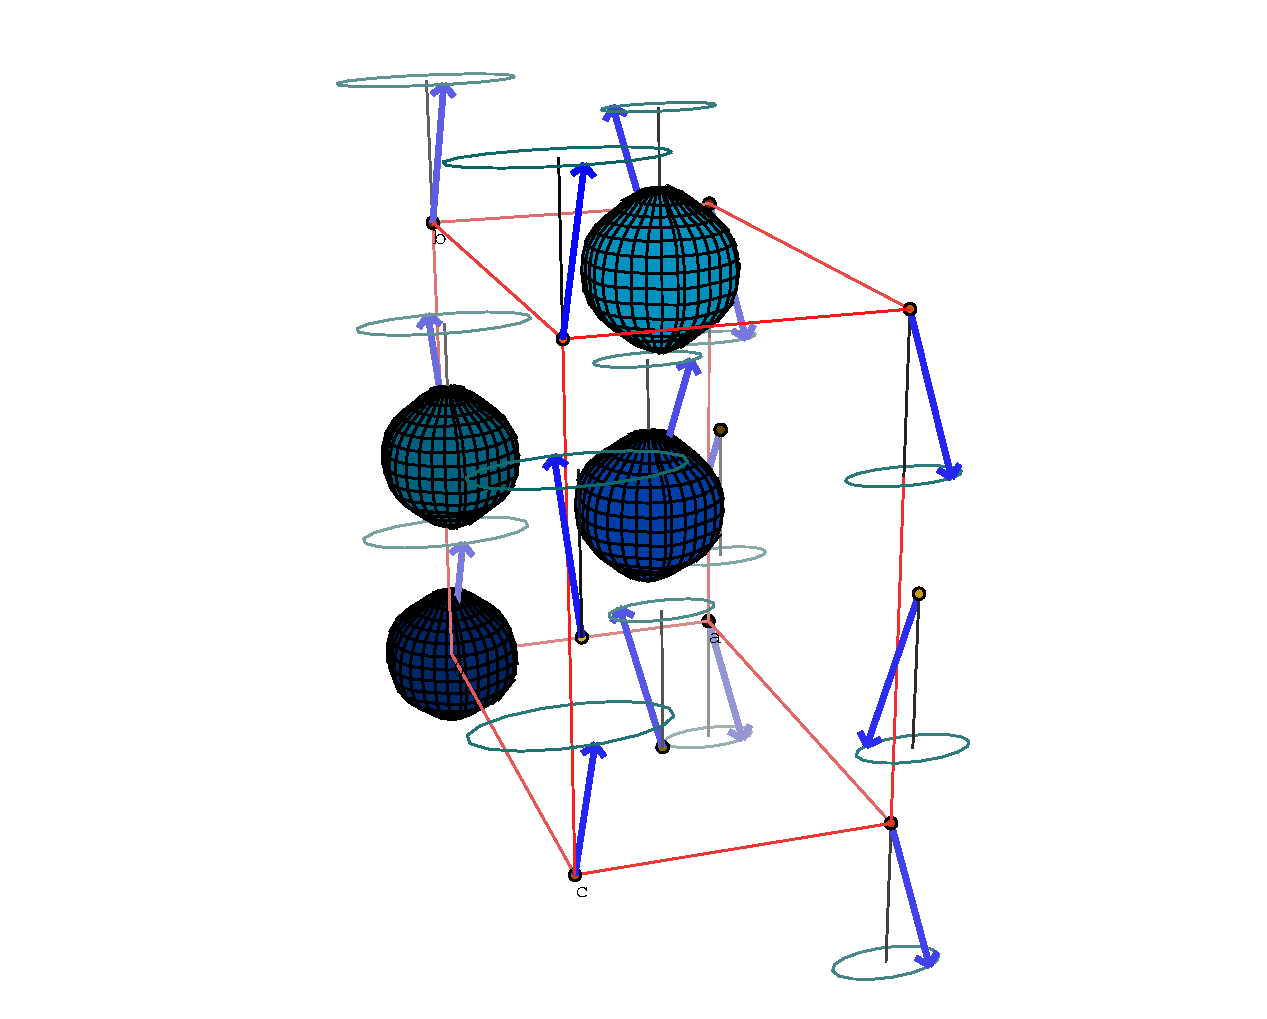
\includegraphics[angle=-0, width=0.6\textwidth]{figsrc/animationAF1.eps}
\end{center}
\caption{NdCu$_2$ - snapshot of animation of the mode 
at Q=(0.67 1 0) at energy 0.7~meV in phase AF1 at 
H=0 and T=1.5~K [plot created by program 
{\prg display\_densities}\index{display\_densities}]
}\label{animationAF1}
\end{figure}

\subsection{Application to Neutron scattering from Interacting Magnetic Ions}
\label{neutronformalism}

We now apply the theory outlined above to the inelastic scattering of neutrons by electrons of magnetic ions
in a crystalline solid. The observable measured here is the
Fourier transform of the magnetisation (=magnetic moment density) operator of a magnetic ion ($\hat \mbf M(\mbf Q)$).
The magnetisation operator consists of a spin and an orbital contribution and thus
its Fourier transform may be written as a sum $\hat \mbf M(\mbf Q)=\hat \mbf M_S(\mbf Q)+\hat \mbf M_L(\mbf Q)$.
For consistency with ref.\cite{lovesey84-1} please note that we write the following formulas 
in terms of the magnetisation operator instead of the scattering operator
$\hat \mathcal Q_{\alpha} \equiv -\hat M_{\alpha}(\mbf Q)/(2\mu_B)$ (where $\alpha=x,y,z$ and $\mu_B$ is the
Bohr magneton).

The general expression for the double differential scattering cross section 
for unpolarised neutrons has been given frequently in literature (see e.g. \cite{lovesey84-1}):

%\begin{eqnarray}
%\frac{d^2\sigma}{d\Omega dE'}&=&N\frac{k'}{k}\left( \frac{\hbar \gamma e^2}{m_e c^2}  \right)^2
%%\sum_{\mbf Q} \delta_{\vec\kappa,\mbf Q}
%\sum_{\alpha\beta=1,2,3}(\delta_{\alpha\beta}- \frac{Q_{\alpha} Q_{\beta}}{|\mbf Q|^2}) 
%S^{\alpha \beta}_{\rm mag}(\mbf Q,\omega)+
%N\frac{k'}{k}S_{\rm nuc}(\mbf Q,\omega) \nonumber \\
%S_{\rm mag}&=&S_{\rm mag}^{\rm el}+S_{\rm mag}^{\rm inel} \label{smag} 
%\end{eqnarray}

%[BETTER USE THE FOLLOWING]
\begin{eqnarray}\label{dsdoderepeated}
\frac{d^2\sigma}{d\Omega dE'}&=&N\frac{k'}{k}\left( \frac{ \gamma r_0}{2 \mu_B}  \right)^2
%\sum_{\mbf Q} \delta_{\vec\kappa,\mbf Q}
\sum_{\alpha\beta=1,2,3}(\delta_{\alpha\beta}- \frac{Q_{\alpha} Q_{\beta}}{|\mbf Q|^2}) 
S^{\alpha \beta}_{\rm mag}(\mbf Q,\omega)+
N\frac{k'}{k}S_{\rm nuc}(\mbf Q,\omega) \nonumber \\
S_{\rm mag}&=&S_{\rm mag}^{\rm el}+S_{\rm mag}^{\rm inel} \label{smag} 
\end{eqnarray}


In (\ref{dsdoderepeated}) $N$ denotes the number of magnetic atoms in the sample, $\mbf k$ and $\mbf k'$ the wave vector %%@
of the incoming and scattered neutron, respectively.
The total magnetic cross section is $4\pi (\gamma r_0)^2=4\pi\left(\frac{\hbar \gamma e^2}{mc^2}\right)^2
=3.65$~barn. 
$\hbar \omega=E-E'$  and
$\mbf Q =\mbf k-\mbf k'$  denote the energy and momentum transfer.
The van Hove scattering functions $S_{\rm mag}$ and $S_{\rm nuc}$ may be split into an elastic and an inelastic part. We %%@
will discuss here only the inelastic magnetic scattering 
function\footnote{
the coherent inelastic nuclear scattering may be treated in a similar way by associating
the observable $\mathcal O$ with $\mathcal O \leftrightarrow b e^{i\mbf Q \mbf u}$,
where $b$ denotes the nuclear coherent scattering length.
}, which is given by

%\begin{eqnarray}
%S_{\rm mag}^{\rm inel,\alpha\beta}(\mbf Q,\omega)&=&\frac{1}{2\pi\hbar}\int_{-\infty}^{+\infty}dt e^{i\omega t}
%\frac{1}{N}\sum_{nn'} e^{-W_r(Q)- W_{r'}(Q)} e^{-i\mbf Q(\mbf R_n-\mbf R_{n'})} \nonumber \\
%&&\times (\langle \hat \mathcal Q^{n \dag}_{\alpha}(t) \hat \mathcal Q^{n'}_{\beta}(0) \rangle_{T,H}
%- \langle \hat \mathcal Q^{n \dag}_{\alpha}\rangle_{T,H} \langle \hat \mathcal Q^{n'}_{\beta} \rangle_{T,H})
%\end{eqnarray}

%[BETTER USE THE FOLLOWING]

\begin{eqnarray}\label{Sinel}
S_{\rm mag}^{\rm inel,\alpha\beta}(\mbf Q,\omega)&=&\frac{1}{2\pi\hbar}\int_{-\infty}^{+\infty}dt e^{i\omega t}
\frac{1}{N}\sum_{nn'} e^{-W_n(Q)- W_{n'}(Q)} e^{-i\mbf Q \cdot (\mbf R_n-\mbf R_{n'})}  \\
&\times& (\langle \hat M_{\alpha}^{n \dag}(t,\mbf Q)  \hat M_{\beta}^{n'}(0,\mbf Q) \rangle_{T,H}
- \langle \hat M^{n \dag}_{\alpha}(\mbf Q)\rangle_{T,H} \langle \hat M^{n'}_{\beta}(\mbf Q) \rangle_{T,H})\nonumber
\end{eqnarray}

In (\ref{Sinel}) the first term in the bracket corresponds to the total and the second term to the elastic
scattering.
If we split the index $n$ into basis and 
lattice part $n=(\Bell,s)$ and 
compare equation~(\ref{sigmass}), we see that %%@
the scattering function depends on the correlation function between the magnetisation operator
$\hat \mbf M(\mbf Q)$, which is the observable in the case of magnetic neutron scattering 
($\mathcal O \leftrightarrow \hat \mbf M(\mbf Q)$).

\begin{equation}\label{sinelmag}
S_{\rm mag}^{\rm inel,\alpha\beta}(\mbf Q,\omega)=
\sum_{ss'}  e^{-W_s(Q)- W_{s'}(Q)} \frac{\hili{\Sigma^{ss'}_{\alpha\beta}}({\mbf Q},\omega)}{2\pi \hbar N_b} 
\end{equation}

 $W_s(Q)$ is  the Debye-Waller
factor of the atom number $s$ in the magnetic unit cell\footnote{In case
of magnetic order. In general this will be the unit cell of 
the Bravais lattice in section~\ref{formalism}, which
is a superlattice of the crystal lattice.}. $N_b$ denotes the number of magnetic
atoms in the magnetic unit cell.
Therefore, if the generalised eigenvalue problem (\ref{evproblem}) for the dynamical matrix
has been solved, the magnetic neutron scattering function can
be  evaluated with the help of equations (\ref{fluctdissbeyond}) and (\ref{Xcalc}):

\begin{eqnarray}\label{sinelmagfinal}
S_{\rm mag}^{\rm inel,\alpha\beta}(\mbf Q,\omega)&=&
\sum_{r,ss'}  
\frac{(\sqrt{\Gamma^s(\mbf Q)})^\ast\sqrt{\Gamma^{s'}(\mbf Q)} 
e^{-W_s(Q)- W_{s'}(Q)}}{N_b(1-e^{-\hbar\hili{\omega^r}(\mbf Q)/kT})} \times \\ \nonumber
&& \times \mathcal V^s_{\alpha1}(\mbf Q)
\hili{ \mathcal T^{sr}}(\mbf Q)\hbar \hili{\omega^r}(\mbf Q)
 \delta(\hbar \hili{\omega^r}(\mbf Q) - 
\hbar \omega) \hili{\mathcal T^{rs'\dag}}(\mbf Q) 
\mathcal V^{s'\dag}_{1\beta}(\mbf Q)
\end{eqnarray}

Once the eigenvectors \hili{$\M{\mathcal T}$} of the system have been determined, this expression can be 
 evaluated. 
Form factor effects on the scattering intensity are
 due to the $\mbf Q$-dependence of the magnetisation operator, which means that
the transformation matrices \hili{$\m{\mathcal V}^s$}
 and the eigenvalues $\Gamma^s$ are also
$\mbf Q$-dependent.  These quantities have
 to be calculated by evaluating the transition
matrix elements\footnote{\hili{using the appropriate 
expression for the matrix elements of of the scattering
operator as given in~\cite[equ. (11.86) or (11.87b)]{lovesey84-1}.}} 
of \hili{$\hat \mbf M(\mbf Q)$ for every 
scattering vector $\mbf Q$ 
and diagonalising the matrix (\ref{mumatrix}) }
with $\mathcal O \leftrightarrow \hat \mbf M(\mbf Q)$.
For small $Q$ this procedure can be simplified by using the dipole approximation,
which is described below.

\subsection{Dipole Approximation}

Frequently the neutron scattering cross section may be calculated 
in the dipole
approximation, which is valid if $1/Q$ is much 
\hili{larger than the spatial dimension of a subsystem, i.e.
 the radius of the electron shell}. 
 Any deviations from spherical symmetry of the magnetic moment density
(due to the crystal electric field) are neglected in this approximation.
In the dipole approximation the scattering operator is written as a product of a form-factor and total angular momentum %%@
operator: 

%\begin{equation}
%\hat \mathcal Q^{n}_{\alpha} \approx \frac{1}{2}[F^n_S(Q) g_S \hat S^{n}_{\alpha} + F^n_L(Q) g_L \hat %L^{n}_{\alpha}]
%\end{equation}

%[BETTER USE]

\begin{equation}
\hat M^{n}_{\alpha}(\mbf Q) \approx -\mu_B[F^n_S(Q) g_S \hat S^{n}_{\alpha} + F^n_L(Q) g_L \hat L^{n}_{\alpha}]
\end{equation}
 
\noindent where the spin and orbital $g$-factors 
are $g_S \approx 2$ and $g_L=1$, respectively. $F_S(Q)=\langle j_0 (Q) \rangle$ and
 $F_L(Q)=\langle j_0 (Q) \rangle + \langle j_2 (Q) \rangle$ are the spin and orbital form factor for the ion $n$, %%@
respectively, whilst $\hat S^{n}_{\alpha}$ and $\hat L^{n}_{\alpha}$ are their total angular momentum operators. We %%@
consider
three cases of the dipole approximation:

\begin{quotation}

%\item[$\hat \mathcal O^{n}_{\alpha} \leftrightarrow \frac{1}{2}
%[BETTER USE]
\item[$\hat M^{n}_{\alpha}(\mbf Q) \leftrightarrow -\mu_B
\{ F^n_S(Q) g_S \hat S^{n}_{\alpha} + F^n_L(Q) g_L \hat L^{n}_{\alpha} \}$ : ]
In this case, the full expression of the dipole approximation is used, whereby the scattering operator is replaced by
%To this level of approximation the observable  is therefore instead of the scattering operator
a linear combination of spin and orbital momentum.

%\item[$\hat \mathcal O^{n}_{\alpha} \leftrightarrow \frac{1}{2}
%[BETTER USE]
\item[$\hat M^{n}_{\alpha}(\mbf Q) \leftrightarrow -\mu_B
F^n_S(Q) g_S \hat S^{n}_{\alpha}$:]
In many magnetic ions the orbital moment is 
zero, so it is sufficient
to consider only the spin momentum. 
This is the case for the half filled shells Gd$^{3+}$, Eu$^{2+}$, or where the orbital moment is
quenched by the crystal field in transition metal ions.

%\item[$\hat \mathcal O^{n}_{\alpha} \leftrightarrow \frac{1}{2}
%[BETTER USE]
\item[$\hat M^{n}_{\alpha}(\mbf Q) \leftrightarrow -\mu_B
 g_J F^n(Q) \hat J_{\alpha}^n$:]
For rare earth based systems the orbital momentum cannot be neglected, however the
spin orbit interaction is very strong so that in many cases it is sufficient to consider
only the ground state multiplet according to Hund's rules. In this approximation the
spin and orbital momentum are both proportional to the total angular momentum $ \hat \mbf J$ and the
magnetisation operator may be written as 
$\hat M^{n}_{\alpha} \approx -\mu_B g_J F^n(Q)  \hat J_{\alpha}^n $ with
the form factor  $F(Q)=\langle j_0 (Q) \rangle + \frac{2-g_J}{g_J}\langle j_2 (Q) \rangle $.
In this approximation the observable is the total angular momentum operator
($g_J$ denotes the Land\'e splitting factor).
\end{quotation}


{\prg mcdisp\index{mcdisp}} automatically calculates the intensity in
dipole approximation and also going beyond, if possible, the result
is stored in file {\prg mcdisp.qei}.




%***********************************************************************************

% NOTE from old manual - perhaps important for option -r in mcdispit
%{\tiny Note: for intermediate coupling schemes (which are introduced into mcdisp by putting $gJ=0$) in 
%dipole approximation the 
%$g_J F(Q)$ have to be substituted with $g_S F_S(Q)=2F_S(Q)=2 \langle j_0 (Q) \rangle$ for the spin components %%@
%($\alpha'=a',c',e'$),
%and with  $g_L F_L(Q)=F_L(Q)=\langle j_0 (Q) \rangle + \langle j_2 (Q) \rangle $ 
%for the spin components ($\alpha'=b',d',f'$) of the scattering function $S$. The $\alpha$ and $\beta$ indices in 
%the polarization factor refer then to  the $a .. a'or b'$,$b ..c'or d'$ and $c .. e'or f'$ components of %%@
%$S_{\alpha'\beta'}$.
%}





\begin{figure}[t]%h=here, t=top, b=bottom, p=separate figure page
\begin{center}\leavevmode
\includegraphics[angle=-0, width=0.6\textwidth]{figsrc/ho2ti2o7diffuse.eps}
\end{center}
\caption{\label{ho2ti2o7diffuse}
Ho$_2$Ti$_2$O$_7$ - calculated diffuse magnetic scattering intensity in the (110)-(001)
 plane at $T=10$~K.
[plot created by program {\prg displaycontour\index{displaycontour}}]
}
\end{figure}

\subsection{Diffuse Scattering}

The program {\prg McDisp} may be used straightforward to calculate quasi elastic intensity
 by

\begin{itemize}
\item
 specification of an energy
range [emin,emax] in file {\prg mcdisp.par\index{mcdisp.par}} which corresponds to the interval of energies (around zero
energy transfer) sensed by the detector of the diffuse scattering experiment. 
\item
 quasi elastic intensity is expected only in the paramagnetic state - thus in {\prg mcdisp.mf\index{mcdisp.mf}} a
 a temperature above the magnetic ordering temperature should be selected.
\item start {\prg mcdisp} in the usual way, using the DMD method.
\end{itemize} 
 
The file {\prg mcdisp.dsigma.tot} produced by the calculation contains the calculated diffuse scattering cross section.
Figure~\ref{ho2ti2o7diffuse} shows an output of such a calculation for the diffuse scattering
on Ho$_2$Ti$_2$O$_7$.

For comparison it is also possible to do a calculation using the option {\prg -r} forcing
 the program {\prg mcdisp\index{mcdisp}} to calculate the cross section
 using the full MF-RPA algorithm (output stored in {\prg mcdisp.dsigma})

\subsection{Powder Neutron Cross Section}


\begin{figure}[tb]%h=here, t=top, b=bottom, p=separate figure page
\begin{center}\leavevmode
\includegraphics[angle=0, width=0.5\textwidth]{figsrc/contour2K_070504.eps}
\end{center}
\caption{Magnetic Neutron powder spectrum of PrNi$_2$B$_2$C for $T=2$~K as calculated using module {\prg powdermagnons} %%@
in combination with {\prg 
mcdisp}.}\label{prni2b2c_2K}
\end{figure}

\begin{figure}[tb]%h=here, t=top, b=bottom, p=separate figure page
\begin{center}\leavevmode
\includegraphics[angle=0, width=0.5\textwidth]{figsrc/contour10K_070504.eps}
\end{center}
\caption{Magnetic Neutron powder spectrum of PrNi$_2$B$_2$C for $T=10$~K  as calculated using module {\prg %%@
powdermagnons} in combination with {\prg 
mcdisp}.}\label{prni2b2c_10K}
\end{figure}

{\prg Mcdisp} in combination with module {\prg powdermagnon} can be used to calculate
powder neutron pattern. In order to do this, a 3-step procedure is required:

\subsubsection{Creation of the q-vector list}
The first step is to create a list of reflections to be used for 
the averaging of the powder neutron cross section. 

just type: powdermagnon 0.3 2 0.1 80

meaning take file {\prg mcphas.j\index{mcphas.j}}, generate a reflection list and put it to 
file {\prg mcdisp.par\index{mcdisp.par}}. Parameters in the above command are 
\begin{itemize}
\item
 0.3 ....qmin   [1/A] minimal q vector
\item
 2   ....qmax   [1/A] maximal q vector
\item
 0.1 ....deltaq [1/A] step width in q
\item
 80  ....number of steps in polar coordinate $\Theta$
        (steps in polar angle $\phi$ are  then calculated in module
        {\prg powdermagnon} by $\delta \phi= \delta \Theta*\pi/(4*sin(\Theta))$
\end{itemize}

\subsubsection{Calculation of the Dispersion using {\prg mcdisp\index{mcdisp}}}

In order to set the correct temperature and $k_f$ (or $k_i$) etc. edit
the input files for module {\prg mcdisp\index{mcdisp}} and start {\prg mcdisp\index{mcdisp}}. Mind 
to select the fast algorithm so that a file {\prg mcdisp.qei} is created.

\subsubsection{Powder-averaging the spectra}
The third and last step in the calculation of the powder pattern is the averaging
of the spectra with the same value of $Q$. This is done by restarting module
{\prg powdermagnon} by: 

powdermagnon -r results\\mcdisp.qei 0.5 30 0.2 

meaning take  results from file {\prg results\\mcdisp.qei} and average the
spectra. Output is printed to the console (STDOUT) and can be piped to a file in
order to print it with {\prg displaycontour\index{displaycontour}}. An example is given in fig.~
\ref{prni2b2c_2K} and \ref{prni2b2c_10K}.
Parameters in the above command  are:
\begin{itemize}
\item 0.5 ....Emin   [meV] minimal energy
\item 30 ....Emax   [meV] maximal energy
\item 0.2....deltaE [meV] energy step width
\end{itemize}


\clearpage

\section{Including Quadrupolar and Higher Order Interactions}
\label{qint}


The module {\prg Cfield} allows also to calculate systems with higher order interactions such
as quadrupolar interactions. Quadrupolar and higher order interactions can be calculated, which
can be described by products of Stevens operators. The general two ion exchange coupling is

\begin{equation}
\label{multipolehamiltonrepeated}
 {\mathcal H}_{JJ}=
             -\frac{1}{2}  \sum_{nn'} \sum_ {ll'} \sum_{mm'}
     {\mathcal K}_{ll'}^{mm'}(nn') O_{lm}({\mbf J}^n) O_{l'm'}({\mbf J}^{n'})
\end{equation}

For further information on the notation and symmetry restrictions to the
parameters in the Hamiltonian refer to~\cite{jensen91-1}~\footnote{\em http://www.nbi.ku.dk/page40667.htm}.


\subsection{Setting up {\prg mcphas.j\index{mcphas.j}} and other input files}

In order to include the higher order interactions, the number of columns in the input file
{\prg mcphas.j\index{mcphas.j}} has to be increased. The additional columns then contain the higher order
exchange constants.

Using the module {\prg Cfield}, the input file {\prg mcphas.j\index{mcphas.j}} may look as given for the 
example GdRu$_2$Si$_2$ in {\prg examples/gdru2si2}:

{\footnotesize
\begin{verbatim}
# GdRu2Si2 anisotropic bilinear and biquadratic exchange 
#<!--mcphase.mcphas.j-->
#***************************************************************
# Lattice and Exchange Parameter file for
# mcphas version 3.0
# - program to calculate static magnetic properties
# reference: M. Rotter JMMM 272-276 (2004) 481
# mcdisp version 3.0
# - program to calculate the dispersion of magnetic excitations
# reference: M. Rotter et al. J. Appl. Phys. A74 (2002) 5751
#***************************************************************
#
# Lattice Constants (A)
#! a=4.165 b=4.165 c=9.654 alpha=  90 beta=  90 gamma=  90
#! r1a= 0.5 r2a=   0 r3a=   0
#! r1b= 0.5 r2b=   1 r3b=   0   primitive lattice vectors [a][b][c]
#! r1c= 0.5 r2c=   0 r3c=   1
#! nofatoms=1  nofcomponents=8  number of atoms in primitive unit cell/number of components of each spin
#****************************************************************************}
#! da=   0 [a] db=   0 [b] dc=   0 [c] nofneighbours=38 diagonalexchange=1 gJ=   2 cffilename=Gd3p_cfield.sipf
# da[a]    db[b]      dc[c]       Jaa[meV]  Jbb[meV]  Jcc[meV]  Jab[meV]  Jba[meV]  Jac[meV]  Jca[meV]  Jbc[meV]  %%@
Jcb[meV]} 
-1.0 0.0 0.0 0.08390 0.08390 0.21890 -0.0024 -0.0096 -0.0008 -0.0096 -0.0024 
1.0 0.0 0.0 0.08390 0.08390 0.21890 -0.0024 -0.0096 -0.0008 -0.0096 -0.0024 
0.0 -1.0 0.0 0.08390 0.08390 0.21890 -0.0024 -0.0096 -0.0008 -0.0096 -0.0024 
0.0 1.0 0.0 0.08390 0.08390 0.21890 -0.0024 -0.0096 -0.0008 -0.0096 -0.0024 
-0.5 -0.5 -0.5 0.00380 0.00380 0.01000 0.0 0.0 0.0 0.0 0.0 
-0.5 -0.5 0.5 0.00380 0.00380 0.01000 0.0 0.0 0.0 0.0 0.0 
-0.5 0.5 -0.5 0.00380 0.00380 0.01000 0.0 0.0 0.0 0.0 0.0 
-0.5 0.5 0.5 0.00380 0.00380 0.01000 0.0 0.0 0.0 0.0 0.0 
0.5 -0.5 -0.5 0.00380 0.00380 0.01000 0.0 0.0 0.0 0.0 0.0 
0.5 -0.5 0.5 0.00380 0.00380 0.01000 0.0 0.0 0.0 0.0 0.0 
0.5 0.5 -0.5 0.00380 0.00380 0.01000 0.0 0.0 0.0 0.0 0.0 
0.5 0.5 0.5 0.00380 0.00380 0.01000 0.0 0.0 0.0 0.0 0.0 
-1.0 -1.0 0.0 -0.03630 -0.03630 -0.09445 0.0 0.0 0.0 0.0 0.0 
-1.0 1.0 0.0 -0.03630 -0.03630 -0.09445 0.0 0.0 0.0 0.0 0.0 
1.0 -1.0 0.0 -0.03630 -0.03630 -0.09445 0.0 0.0 0.0 0.0 0.0 
1.0 1.0 0.0 -0.03630 -0.03630 -0.09445 0.0 0.0 0.0 0.0 0.0 
1.5 -0.5 0.5 -0.00072 -0.00072 -0.00188 0.0 0.0 0.0 0.0 0.0 
-1.5 -0.5 0.5 -0.00072 -0.00072 -0.00188 0.0 0.0 0.0 0.0 0.0 
1.5 -0.5 -0.5 -0.00072 -0.00072 -0.00188 0.0 0.0 0.0 0.0 0.0 
0.5 -1.5 0.5 -0.00072 -0.00072 -0.00188 0.0 0.0 0.0 0.0 0.0 
0.5 1.5 0.5 -0.00072 -0.00072 -0.00188 0.0 0.0 0.0 0.0 0.0 
0.5 1.5 -0.5 -0.00072 -0.00072 -0.00188 0.0 0.0 0.0 0.0 0.0 
-0.5 1.5 0.5 -0.00072 -0.00072 -0.00188 0.0 0.0 0.0 0.0 0.0 
-1.5 -0.5 -0.5 -0.00072 -0.00072 -0.00188 0.0 0.0 0.0 0.0 0.0 
1.5 0.5 0.5 -0.00072 -0.00072 -0.00188 0.0 0.0 0.0 0.0 0.0 
-1.5 0.5 -0.5 -0.00072 -0.00072 -0.00188 0.0 0.0 0.0 0.0 0.0 
-0.5 -1.5 -0.5 -0.00072 -0.00072 -0.00188 0.0 0.0 0.0 0.0 0.0 
-0.5 -1.5 0.5 -0.00072 -0.00072 -0.00188 0.0 0.0 0.0 0.0 0.0 
1.5 0.5 -0.5 -0.00072 -0.00072 -0.00188 0.0 0.0 0.0 0.0 0.0 
-0.5 1.5 -0.5 -0.00072 -0.00072 -0.00188 0.0 0.0 0.0 0.0 0.0 
-1.5 0.5 0.5 -0.00072 -0.00072 -0.00188 0.0 0.0 0.0 0.0 0.0 
0.5 -1.5 -0.5 -0.00072 -0.00072 -0.00188 0.0 0.0 0.0 0.0 0.0 
-2.0 0.0 0.0 -0.01754 -0.01754 -0.04567 0.0 0.0 0.0 0.0 0.0 
2.0 0.0 0.0 -0.01754 -0.01754 -0.04567 0.0 0.0 0.0 0.0 0.0 
0.0 -2.0 0.0 -0.01754 -0.01754 -0.04567 0.0 0.0 0.0 0.0 0.0 
0.0 2.0 0.0 -0.01754 -0.01754 -0.04567 0.0 0.0 0.0 0.0 0.0 
0.0 0.0 1.0 0.24850 0.24850 0.13560 0.0 0.0 0.0 0.0 0.0 
0.0 0.0 -1.0 0.24850 0.24850 0.13560 0.0 0.0 0.0 0.0 0.0 
\end{verbatim}
}
here the meaning of the Jaa, Jbb, Jcc, Jdd, Jee \dots is the exchange ${\mathcal K}_{ll'}^{mm'}(ss')$ between %%@
$O_1^1(s)$, $O_1^0(c)$,$O_1^1(c)$, $O_2^2(s)$, $O_2^1(s)$,$O_2^0(c)$,$O_2^1(c)$,$O_2^2(c)$,$O_3^3(s)$, ...
according to equation table~\ref{olms}.
 The exchange constants for the
products of these Stevens operators have to be 
given according to the following scheme:

\begin{verbatim}
   aa bb cc ab ba ac ca bc cb (3x3 matrix)
   aa bb cc dd ab ba ac ca ad da bc cb bd db cd dc (4x4 matrix)
   aa bb cc dd ee ab ba ac ca ad da ae ea bc cb bd db be eb cd dc ce ec de ed (5x5 matrix)
   etc ...
\end{verbatim}

The other input and output files have the same format as usual, but with the modification, that
there are now $n$ components of the 'spins' instead of 3 ($<J_a>$,$<J_b>$,$<J_c>$).
The components $<J_a>$,$<J_b>$,$<J_c>$,$<J_d>$,$<J_e>$, etc. correspond to $<O_{11}(s)>$, $<O_{10}>$,
$<O_{11}>$, $<O_{22}(s)>$, $<O_{21}(s)>$,$<O_{20}>$,$<O_{21}>$,$<O_{22}>$,$<O_{33}(s)>$, ...
 respectively. Table~\ref{olms} contains a list of first and second order Stevens parameters.
For a full list please refer to appendix~\ref{stevens}.

\begin{table}[hb] 
\begin{center}  
\caption {Stevens operator equivalents $O_l^m$ and corresponding notation used in module {\prg %%@
cfield\index{cfield}} 
($J_{\pm}=J_x\pm iJ_y=J_c\pm iJ_a$ ). For a full list please refer to appendix~\ref{stevens}.}   
\label{olms}   
\begin{tabular} 
{lr} 
Stevens Operator & Notation used in module {\prg cfield\index{cfield}} \\
\hline
$O_{00}=1$ ($O_0^0(s)=0$) &\\
\hline
$O_{11}(s)=\frac{-i}{2}[J_+-J_-]=J_y$ &  $J_a$\\
$O_{10}=J_z$  ($O_1^0(s)=0$) & $J_b$ \\
$O_{11}=\frac{1}{2}[J_++J_-]=J_x$ &  $J_c$\\
\hline
$O_{22}(s)=\frac{-i}{2}[J_+^2-J_-^2]=J_xJ_y+J_yJ_x$($=2P_{xy}$) & $J_d$ \\
$O_{21}(s)=\frac{-i}{4}[(J_+-J_-)J_z+J_z(J_+-J_-)]=\frac{1}{2}[J_yJ_z+J_zJ_y]$($=P_{yz}$) & $J_e$ \\
$O_{20}=[3J_z^2-J(J+1)]$ ($O_2^0(s)=0$) & $J_f$ \\
$O_{21}=\frac{1}{4}[(J_++J_-)J_z+J_z(J_++J_-)]=\frac{1}{2}[J_xJ_z+J_zJ_x]$($=P_{xz}$) & $J_g$ \\
$O_{22}=\frac{1}{2}[J_+^2+J_-^2]=[J_x^2-J_y^2]$ & $J_h$ \\
\hline
 \end{tabular}
\end{center}   
\end{table}

The {\prg indexexchange} parameter discussed in section~\ref{mcphasj} may be useful in keeping the input
of the exchange components short. For example the $\zeta$ and $\eta$ strain modes on the quasi-cubic sites
of a double hexagonal close packed structure involves the coupling of $P_{zx}$ ($J_g$) and $P_{xy}$ ($J_d$) 
as well as $P_{yz}$ ($J_e$) and $O_2^2$ $(J_h)$ quadrupoles, so the {\prg diagonalexchange=1} option 
cannot be used. Thus 64 components need to be specified to describe the $8\times 8$ exchange tensor. 
However, we can simplify this with the {\prg indexexchange} parameter by setting {\prg diagonalexchange=2}, 
as follows for UPd$_3$:

{\footnotesize \begin{verbatim}
# UPd3 
#<!--mcphase.mcphas.j-->
#! a=9.92465 b=5.73 c=9.65  alpha=  90 beta=  90 gamma=  90
#! r1x= 1 r2x=   0 r3x=   0
#! r1y= 0 r2y=   1 r3y=   0
#! r1z= 0 r2z=   0 r3z=   1
#! nofatoms=1 nofcomponents=8
#*************************************************************************
#! x=   0 [a] y=   0 [b] z=   0 nofneighbours=6 diagonalexchange=2 gJ=0.8 cffilename=mcphas.cf1
#! x[a]  y[b]    z[c]   Ja[meV]  Jb[meV]  Jc[meV]  Jd[meV]  Je[meV]  Jf[meV]  Jg[meV]  Jh[meV]
#! symmetricexchange=1 indexexchange= JaJa JbJb JcJc JdJd JeJe JfJf JgJg JhJh JgJd JhJe
 0    0    0.5 -0.022 -0.022 -0.022  0.0035198 -0.18643  -0.00053332 -0.18643   0.00087996  0.013      0.0064378
 0    0   -0.5 -0.022 -0.022 -0.022  0.0035198 -0.18643  -0.00053332 -0.18643   0.00087996  0.013      0.0064378
 0.5  0.5  0   -0.022 -0.022 -0.022 -0.0034195 -0.019714 -0.00034044 -0.019714 -0.00085486 -0.0065221 -0.0050197
-0.5 -0.5  0   -0.022 -0.022 -0.022 -0.0034195 -0.019714 -0.00034044 -0.019714 -0.00085486 -0.0065221 -0.0050197
 0.5 -0.5  0   -0.022 -0.022 -0.022 -0.0034195 -0.019714 -0.00034044 -0.019714 -0.00085486 -0.0065221 -0.0050197
-0.5  0.5  0   -0.022 -0.022 -0.022 -0.0034195 -0.019714 -0.00034044 -0.019714 -0.00085486 -0.0065221 -0.0050197
\end{verbatim} }

\subsection{Running {\prg McPhase} and {\prg McDisp}}

The programs {\prg mcphas} and {\prg mcdisp\index{mcdisp}} are run completely the same way as usual, only
the output files contain also information about the (thermal) expectation values of $<O_l^m>$
dependent on temperature and magnetic field. 
Using the module cfield the notation $<J_a>$,$<J_b>$,$<J_c>$,
$<J_d>$, $<J_e>$, etc. correspond to $<O_{11}(s)>$, $<O_{10}>$,
$<O_{11}>$, $<O_{22}(s)>$, $<O_{21}(s)>$,$<O_{20}>$,$<O_{21}>$,$<O_{22}>$,$<O_{33}(s)>$, ...
 respectively.
Note that by the higher order interactions not only the static properties are changed, but also the
dispersion of the magnetic excitations is influenced.


The directory {\prg examples/gdru2si2} contains an example of a simulation of biquadratic (i.e. isotropic %%@
quadrupolar) interactions leading to an improved description of magnetic susceptibility.

For DyCu$_2$ the conversion
of the magnetic axis due to quadrupolar exchange has been calculated according to the model 
\cite{yoshida98-1421}. The calculated quadrupolar phase diagram is shown in figure~\ref{qphased}.

\begin{figure}[hb]%h=here, t=top, b=bottom, p=separate figure page
\begin{center}\leavevmode
\includegraphics[angle=-90, width=0.5\textwidth]{figsrc/dyphased.ps}
\end{center}
\caption{DyCu$_2$: calculated quadrupolar phased diagram. When applying a large magnetic field
parallel to the $c$ axis of the orthorhombic crystal, the system undergoes a structural transformation
associated with a reorientation of the structural unit cell. This effect can be modelled by a large
quadrupolar interaction.[plot created with program {\prg phased}]}
\label{qphased}
\end{figure}

When large  quadrupolar interactions are present, the excitation spectrum is changed and
quadrupolar modes (orbitons) with a finite dispersion are expected. 
These modes correspond to an cooperative oscillation of the quadrupolar moments such as shown
in figure~\ref{qmodes}.
The program {\prg mcdisp\index{mcdisp}}
is able to calculate this dispersion and the corresponding neutron scattering cross section as shown
in figure~\ref{qintensity} for the case of PrCu$_2$. 
 

\begin{figure}[hb]%h=here, t=top, b=bottom, p=separate figure page
\begin{center}\leavevmode
\includegraphics[angle=0, width=0.6\textwidth]{figsrc/orbiton.ps}
\end{center}
\caption{Orbital excitations viewed  as correlated changes in 4f-charge densities.}
\label{qmodes}
\end{figure}

\begin{figure}[hb]%h=here, t=top, b=bottom, p=separate figure page
\begin{center}\leavevmode
\includegraphics[angle=0, width=0.5\textwidth]{figsrc/prcu2_0k0_5T.eps}
\end{center}
\caption{PrCu$_2$: calculated dispersion of quadrupolar excitations in a field of 5 Tesla parallel to the $a$ axis %%@
of this orthorhombic system.
[plot created with program {\prg displaycontour\index{displaycontour}}]}
\label{qintensity}
\end{figure}


\clearpage

\section{Including Phonons and Crystal-Field Phonon interactions}\label{phonons}

In this section we discuss, how lattice dynamics may be considered in the framework of
the Hamiltonian (\ref{fullhamiltonian}). We will see that this corresponds 
to a system of coupled Einstein oscillators. One such oscillator can be modelled 
by setting up a {\prg sipf} file with the module {\prg phonon}. Coupling has
to be done in {\prg mcdisp.j}. Rephrasing lattice dynamics in this way allows 
to couple phonons to the crystal field.

A three dimensional Einstein oscillator (for atom $n$) in a solid can be described by 
the following Hamiltonian

\begin{equation}\label{einstein}
H_E(n)=\frac{a_0^2{\mbf p_n}^2}{2m_n} + \frac{1}{2} {\mbf u}^T_n \m{K}(nn) {\mbf u}_n
\end{equation}

Here $\mbf u$ is the dimensionless displacement vector ($\mbf u_n={\mbf P}_n/a_0=\Delta {\mbf r}_n/a_0$, 
with the Bohr radius $a_0=0.5219$~\AA), $m_n$ the
mass of the atom $n$, $\mbf p_n=d\mbf u_n/dt$ the conjugate momentum to $\mbf u_n$ and
$\m{K}(nn)$ the Matrix describing the restoring force.

Coupling such oscillators leads to the Hamiltonian

\begin{equation}
H_{phon}=\sum_n H_E(n) -\frac{1}{2} \sum_{n\neq n'} {\mbf u}_n^T \m{K}(nn')  {\mbf u}_{n'}
\end{equation}

In a mean field type of theory 
the phonon single ion module has thus to solve the Hamiltonian

\begin{equation}\label{phonsiham}
H_E=\frac{a_0^2{\mbf p}^2}{2m} + \frac{1}{2} {\mbf u}^T \m{K} {\mbf u} - {\mbf F}^T {\mbf u}
\end{equation}

Here the force $\mbf F$ corresponds to the exchange field $\mbf H_{xc}$ and $\mbf u$ to
 the general operator $\mbf I$ and $\m{K}(nn')$ to $\mathcal J(nn')$ of equation (\ref{fullhamiltonian}),
respectively. The single ion Hamiltonian (\ref{phonsiham}) can be solved by transforming
it to normal coordinates (main axis of the Einstein oscillator) using the transformation
matrix $\m{S}$, which diagonalises $\m{K}=\m{S}^T\m{\Omega}\m{S}$:

\begin{equation}
 \mbf u'=\m{S} \mbf u -\m{\Omega}^{-1} \m{S} \mbf F
\end{equation}

\begin{equation}\label{phonsihamdiag}
H_E=\frac{a_0^2{\mbf p'}^2}{2m}+\frac{1}{2} {\mbf u'}^T \m{\Omega} {\mbf u'} 
-\frac{1}{2}\mbf F^T \m{S}^T \m{\Omega}^{-1} \m{S} \mbf F
\end{equation}

Due to the action of the force $\mbf F$ the equilibrium position of the oscillator
is $\mbf u_0=\m{S}^T\m{\Omega}^{-1}\m{S}\mbf F$ (it is the task of the function
{\prg Icalc} to return this equilibrium position), the energies correspond to the three elements
of the diagonal matrix $\m{\Omega}$, i.e. $\Omega_{11}=m a_0^2 (\Delta_1 /\hbar)^2$,
$\Omega_{22}=m a_0^2 (\Delta_2 /\hbar)^2$,
$\Omega_{33}=m a_0^2 (\Delta_3 /\hbar)^2$. In order to run {\prg mcdisp} we
have to calculate the transition matrix elements:

The single ion susceptibility for such a transition, e.g. $\Delta_1$ - corresponds to

\begin{eqnarray}
\m{\chi}^0&=&\sum_{\nu\mu}\frac{\langle \nu|\mbf u|\mu\rangle\langle \mu |\mbf u^T|\nu \rangle}{\Delta_1 -\hbar \omega}
(p_{\nu} -p_{\mu}) \\
&=&\sum_{\nu\mu}\frac{\langle \nu|\m{S}^T \mbf u'|\mu\rangle\langle \mu |\mbf u'^T \m{S}|\nu \rangle}{\Delta_1 -\hbar \omega}
(p_{\nu} -p_{\mu}) 
\end{eqnarray}
Because the different components of $\mbf u'$ commute and the Hamiltonian (\ref{phonsihamdiag})
is separable, for the transition $\Delta_1$ only the terms with $u_1'$ in the nominator
contribute:

\begin{eqnarray}
\chi^0_{\alpha\beta}&=&S^T_{\alpha1}\sum_{\nu\mu}\frac{\langle \nu|u_1'|\mu\rangle\langle \mu | u_1'|\nu \rangle}{\Delta_1 -\hbar \omega}
(p_{\nu} -p_{\mu}) S_{1\beta}\\
&=& S^T_{\alpha1}S_{1\beta}\frac{\hbar^2}{2ma_0^2\Delta_1}\left(\frac{1}{\Delta_1-\hbar\omega}+\frac{1}{\Delta_1+\hbar\omega}\right )
\end{eqnarray}

In order to derive the last result we had to express $u_1'$ in terms of ladder  operators
$u_1'=a_0^{-1} \hbar/\sqrt{2m\Delta_1}(a+a^{\dagger})$ and  apply $a^{\dagger}|\nu\rangle=\sqrt{\nu+1}|\nu+1\rangle$,
$a|\nu\rangle=\sqrt{\nu}|\nu-1\rangle$ and $\sum_{\nu=0}^{\infty}(p_{\nu}-p_{\nu+1})(\nu+1)=1$,
$p_{\nu}=exp(-\nu\Delta_1/kT)(1-exp(-\Delta_1/kT))$. This shows that the single ion susceptibility
of our atom can be written as a sum of three effective transitions (with temperature independent
susceptibility)

\begin{eqnarray}
\chi^0_{\alpha\beta}
&=& \sum_{i=1,2,3} S^T_{\alpha i}S_{i\beta}\frac{\hbar^2}{2ma_0^2\Delta_i}
\left(\frac{1}{\Delta_i-\hbar\omega}+\frac{1}{\Delta_i+\hbar\omega}\right )
\end{eqnarray}

Thus the module {\prg phonon} has to provide in it's function {\prg du1calc} these three
transitions (=number of transitions).

\subsection{Using Single Ion Module {\prg phonon}}

The module {\prg phonon} allows to consider the phononic degrees of freedom in McPhas.
The single ion input file for an oscillating atom has to have the following format:

\begin{verbatim}
#!MODULE=phonon
#<!--mcphase.sipf-->
#
# phonon
# MODPAR1=mass of atom in units of m0 (atomic mass unit=1.660539e-27 kg)
#
#-----------
MODPAR1=57  # mass in(m0)
MODPAR2=7   # Kxx
MODPAR3=7   # Kyy
MODPAR4=8   # Kzz
MODPAR5=0   # Kxy  in (meV)
MODPAR6=0   # Kxz
MODPAR7=0   # Kyz

#-------------------------------------------------------
# Neutron Scattering Length (10^-12 cm) (can be complex)
#-------------------------------------------------------
SCATTERINGLENGTHREAL=0.769
SCATTERINGLENGTHIMAG=0
#  ... note: - if an occupancy other than 1.0 is needed, just reduce 
#              the scattering length linear accordingly

SCATTERINGLENGTHREAL=0.945
SCATTERINGLENGTHIMAG=0
\end{verbatim}

Thus the single ion property file contains the matrix $\m{K}(nn)$, the matrix $\m{K}(nn')$ decribing the
forces between
different ions $n$ and $n'$ have to be given in the file {\prg mcphas.j}, which could
look like:

\begin{verbatim}
# 
#<!--mcphase.mcphas.j-->
*************************************************************
# Lattice Constants (A)
#! a=4.047 b=4.047 c=9.612 alpha=  90 beta=  90 gamma=  90
#! r1a=   1 r2a=   0 r3a= 0.5
#! r1b=   0 r2b=   1 r3b= 0.5   primitive lattice vectors [a][b][c]
#! r1c=   0 r2c=   0 r3c= 0.5
#! nofatoms=1  nofcomponents=3  number of atoms in primitive unit cell/number of components of each spin
#*********************************************************************
#! da=   0 [a] db=   0 [b] dc=   0 [c] nofneighbours=2 diagonalexchange=1 sipffilename=phonon.sipf
#da[a]   db[b]     dc[c]       Jaa[meV]  Jbb[meV]  Jcc[meV]  Jab[meV]  Jba[meV]  Jac[meV]  Jca[meV]  Jbc[meV]  Jcb[meV]
0 0 1 1.1 1.1 1.1
0 0 -1 1.1 1.1 1.1 
#*********************************************************************
\end{verbatim}

It is planned that these files should be created automatically from the 
output of DFT programs. [to be done]

If crystal field - phonon coupling is to be input, magnetic ions may be added to {\prg mcphas.j}.
They should not be placed at exactly the same position as the phonon atoms - i.e. da db dc should be chosen
(slightly) different to enable the mcphas.j loader to identify which  is which.

The coupling between phononic and crystal field degrees of freedom should be derived from
$H_{cf-phon}=(\mbf \nabla_{\mbf u(n')} B_l^m(n))   \mbf u(n')  O_l^m(\mbf J_n)$. This could be done
using the program {\prg pointc} and {\prg makenn} applying small differential changes to
the atomic positions in the unit cell in order to evaluate the gradient of the crystal field
parameters. [efficient program to do this task is to be written]


\section{Single Ion Modules}\label{simod}

In table~\ref{simodtable} the different single ion modules are listed
together with the functionality in the context of programs
{\prg mcphas},{\prg mcdiff} and {\prg mcdisp}.

Usually, internal single ion modules are used as a starting point.
Alternatively, the single ion properties can be calculated by a program
module which has to be written in {\prg c}. Details about this can be found 
in chapter \ref{extsimod}. Several external modules are supplied also
with the program package.

\begin{table}[htb] 
\begin{center}  
\caption {Single ion\index{singleion} modules and functionality in the context of programs
{\prg mcphas},{\prg mcdiff} and {\prg mcdisp}.}   
\label{simodtable}   
\begin{tabular} 
{l|l|l|l} 
module / functionality       &{\prg mcphas} & {\prg mcdiff} & {\prg mcdisp} \\
\hline
INTERNAL MODULES  & & &\\
\hline
{\prg so1ion}                & ok           &  ok           & ok \\
{\prg cfield}                & ok           &  ok           & ok \\
$F(Q)$- go beyond dip approx & -            &  ok           & in test\\
\hline
{\prg kramer} & ok &  ok   & ok \\
\hline
{\prg brillouin} & ok  & ok &  ok\\
\hline
\hline
EXTERNAL MODULES & &  &\\
\hline
{\prg examples/cecu2a/1ion\_mod/kramer.so}  & ok & & ok \\
\hline
{\prg examples/dyni2b2c/1ion\_mod/quartett.so}  & ok & &\\
\hline
{\prg examples/erni2b2c/1ion\_mod/quartett.so}  & ok & &\\
\hline
{\prg examples/gdni2b2c/1ion\_mod/brillouin.so}  & ok & & in test \\
\hline
{\prg examples/ndcu2b\_1dim/1ion\_mod/kramer.so}  & ok & &\\
\hline
{\prg ic1ion} & in test  &  in test          & in test \\
{\prg icf1ion} & in test  &  in test          & in test \\
$F(Q)$- go beyond dip approx        & -        &  in test          & in test \\
\hline
{\prg bin/cf1ion\_module/cfield.so} & ok &  & ok\\
 \end{tabular}
\end{center}   
\end{table}

The filename given for each atom in {\prg mcphas.j\index{mcphas.j}}
or {\prg mcdiff.in\index{mcdiff.in}} determines, which single ion module 
is to be used for a specific ion in the calculation.
As internal single ion modules there are currently available an isotropic spin (internal module {\prg brillouin}, %%@
see
appendix ~\ref{brillouin}), an 
 anisotropic doublet (internal module {\prg kramers}, see appendix ~\ref{kramers}), 
and the rare earth crystal field (internal module {\prg so1ion\index{so1ion}} and
cfield, see section~\ref{cfield}).

\vspace{0.5cm} 
{\bf Internal Single Ion Property Modules:} 
\begin{quote}
\item[{\prg brillouin}]
If the internal module {\prg brillouin}
 (Brillouin function used for single ion properties,
  see appendix ~\ref{brillouin}) is used,
the single ion property file must start with
\begin{verbatim}#!brillouin\end{verbatim} and
the corresponding spin
 quantum number $J$ has to be given in the first uncommented
lines.
Here is an example:
\begin{verbatim}
#!MODULE=brillouin
#<!--mcphas.sipf-->
# single ion parameter file for Gd
J = 3.5
\end{verbatim}
\item [{\prg kramer}] If the internal module {\prg kramers} (anisotropic doublet ground state, see appendix %%@
~\ref{kramers}) is used,
the single ion property file must start with
\begin{verbatim}#!kramer\end{verbatim} and
the corresponding saturation magnetisations have to be given in the first uncommented
line.
Here is an example:
\begin{verbatim}
#!MODULE=kramer
#<!--mcphas.sipf-->
# single ion parameter file for CeCu2
paramnames= |<+|Ja|->| |<-|Jb|->| |<+|Jc|->|
params= 1.6 0.58333   1.1
\end{verbatim}
\item[{\prg so1ion\index{so1ion}}]In order to use the rare earth crystal field module the first line should read
\begin{verbatim}#!MODULE=so1ion\end{verbatim}

then the ion name should be given followed by a list of nonzero crystal field parameters

\begin{verbatim}
#!MODULE=so1ion
#<!--mcphase.sipf-->
 IONTYPE=Ce3+
 B20=  0.1e-1                                           
 B22  =  -0.3e-1                                       
 B40  =  0.0
 B42  =  0.0
 B44  =  0.0
 B60  =  0.0
 B62  =  0.0
 B64  =  0.0
 B66  =  0.0
\end{verbatim}

 - for a description of this module refer
to section~\ref{cfield}.
\end{quote}

In addition to the basic parameters described above the single ion property file 
may/should contain additional parameters as described below. 

\subsection{Land\'e Factor}

In order to calculate the magnetisation and Zeeman term, the Land\'e factor
has to be entered in the single ion property file. For a rare earth ion this
factor gives the ratio of negative angular momentum / magnetic moment.
Note, for intermediate coupling schemes this factor has no meaning (should be set to zero).

\begin{verbatim}
#Lande Factor
GJ=0.85714
\end{verbatim}


\subsection{Magnetic Formfactor Coefficients}

For the more accurate calculation of neutron intensities it is
necessary to give the magnetic form factor (see the table in appendix~\ref{ffacts})
in the single ion property input file. This can
easily be don by adding some additional lines to a single ion property file:

{\footnotesize
\begin{verbatim}
#--------------------------------------------------------------------------------------
# Neutron Magnetic Form Factor coefficients - thanks to J Brown
#   d = 2*pi/Q      
#   s = 1/2/d = Q/4/pi   
#   sin(theta) = lambda * s
#   r= s*s = Q*Q/16/pi/pi
#
#   <j0(Qr)>=   FFj0A*EXP(-FFj0a*r) + FFj0B*EXP(-FFj0b*r) + FFj0C*EXP(-FFj0c*r) + FFj0D
#   <j2(Qr)>=r*(FFj2A*EXP(-FFj2a*r) + FFj2B*EXP(-FFj2b*r) + FFj2C*EXP(-FFj2c*r) + FFj2D
#   <j4(Qr)>=r*(FFj4A*EXP(-FFj4a*r) + FFj4B*EXP(-FFj4b*r) + FFj4C*EXP(-FFj4c*r) + FFj4D
#   <j6(Qr)>=r*(FFj6A*EXP(-FFj6a*r) + FFj6B*EXP(-FFj6b*r) + FFj6C*EXP(-FFj6c*r) + FFj6D
#
#   Dipole Approximation for Neutron Magnetic Formfactor:
#        -Spin Form Factor       FS(Q)=<j0(Q)>
#        -Angular Form Factor    FL(Q)=<j0(Q)>+<j2(Q)>
#        -Rare Earth Form Factor F(Q) =<j0(Q)>+<j2(Q)>*(2/gJ-1)

#--------------------------------------------------------------------------------------
FFj0A=0.0540 FFj0a=25.0293 FFj0B=0.3101 FFj0b=12.1020 FFj0C=0.6575 FFj0c=4.7223 FFj0D=-0.0216
FFj2A=0.6751 FFj2a=18.3421 FFj2B=1.6272 FFj2b=7.2600 FFj2C=0.9644 FFj2c=2.6016 FFj2D=0.0150
FFj4A=-0.4053 FFj4a=+14.0141 FFj4B=+0.0329 FFj4b=+7.0046 FFj4C=+0.3759 FFj4c=+1.7074 FFj4D=+0.0209
FFj6A=-0.0416 FFj6a=+8.0136 FFj6B=-0.1261 FFj6b=+4.0399 FFj6C=+0.1400 FFj6c=+1.0873 FFj6D=+0.0102
\end{verbatim}
}
In order to go beyond the dipolar approximation for the magnetic formfactor in case
of rare earth ions and using module {\prg so1ion} the coefficients $Z(K')$ have to
be given (see appendix~\ref{zk} for values):
{\footnotesize
\begin{verbatim}
#----------------------------------------------------------------------
# coefficients of Z(K') according to Lovesey (Neutron Scattering) vol.2
# chapter 11.6.1 page 233
#  ... these coefficients are needed to go beyond dipolar approx.
#      for the neutron magnetic formfactor in rare earth ions
#----------------------------------------------------------------------
Z1c0=+1.63636364  Z1c2=+2.95041322
		  Z3c2=-0.20896503  Z3c4=-0.25329095
				    Z5c4=+0.03820789  Z5c6=+0.14258681
						      Z7c6=-0.00614959
\end{verbatim}
}

\subsection{Debye Waller Factor}

For the more accurate calculation of neutron intensities it is
necessary to give the magnetic form factor (see the table in appendix~\ref{ffacts})
and the Debye Waller Factor in the single ion property input file. This can
easily be don by adding some additional lines to a single ion property file:
{\footnotesize
\begin{verbatim}
#-------------------------------------------------------
# Debye-Waller Factor: sqr(Intensity)~|sf|~EXP(-2 * DWF *s*s)=EXP (-W)
#                      with s=sin(theta)/lambda=Q/4pi
# relation to other notations: 2*DWF=Biso=8 pi^2 <u^2>
# unit of DWF is [A^2]
#-------------------------------------------------------
DWF=0.4
\end{verbatim}
}

\subsection{Nuclear Neutron Scattering Length}

In order to calculate nuclear neutron intensities properly, {\prg mcdiff} has to
be provided with the neutron scattering length in units of $10^{-14}$~m.
{\footnotesize
\begin{verbatim}
#-------------------------------------------------------
# Neutron Scattering Length (10^-12 cm) (can be complex)
#-------------------------------------------------------
SCATTERINGLENGTHREAL=0.769
SCATTERINGLENGTHIMAG=0
#  ... note: - if an occupancy other than 1.0 is needed, just reduce 
#              the scattering length linear accordingly
\end{verbatim}
}

\subsection{Radial Wavefunction}

In order to calculate the charge density correctly (programs {\prg charges, chrgplt}) and
to evaluate the pointcharge model (program {\prg pointc}) the radial wave function has to be entered in the %%@
parametrization of Clementi and Roetti:
{\footnotesize
\begin{verbatim}
#------------------------------------------------------------------------------------------------------
# radial wave function parameters R_Np,XIp(r)= r^(Np-1) . exp(-xi r) . (2 XIp)^(Np+0.5) / sqrt(2Np!)  
# values tabulated in clementi & roetti Atomic data and nuclear data tables 14 (1974) 177-478
# Co2+ is isoelectronic to Fe+, looking at page  422 of Clemente & Roetti 
# the 3D radial wave function is expanded as R(r)=sum_p C_p R_Np,XIp(r)
#------------------------------------------------------------------------------------------------------
N1=3 XI1=4.95296 C1=0.36301 
N2=3 XI2=12.2963 C2=0.02707 
N3=3 XI3=7.03565 C3=0.14777
N4=3 XI4=2.74850 C4=0.49771 
N5=3 XI5=1.69027 C5=0.11388 
\end{verbatim}
}

The radial wavefunction may be calculated numerically using the program {\prg radwavfunc}\index{radwavfunc}.

\subsection{Radial Matrix Elements}

For the program {\prg pointc} alternatively, the radial matrix elements can be given:
{\footnotesize
\begin{verbatim}
#---------------------------------------------------------
# Radial Matrix Elements (e.g. Abragam Bleaney 1971 p 399)
#---------------------------------------------------------
#<r^2> in units of a0^2 a0=0.5292 Angstroem
R2=1.114
#<r^4> in units of a0^4 a0=0.5292 Angstroem
R4=2.91
#<r^6> in units of a0^6 a0=0.5292 Angstroem
R6=15.03
\end{verbatim}
}



\section{All about External Single Ion Modules}\label{extsimod}

Single ion properties can be described in a very flexible way by
user programmed single ion module functions, which are loaded at runtime.

The first line in such a single ion property file
must contain the filename of the loadable module, in the following example
the file {\prg ./1ion\_mod/kramer.so}:

\begin{verbatim}
#!./1ion_mod/kramer.so
#<!--mcphas.sipf-->
# single ion parameter file for CeCu2
# there follow some module parameters (up to 9) which are 
# loaded at initialisation of the module
nof_electrons=1
MODPAR1=1.6
MODPAR2=0.58333
MODPAR3=1.1

...
\end{verbatim}


If the first line refers not to an internal module, but to
 a loadable module file, the single ion
properties are calculated using functions in this module file.

In the following sections the different functions are presented
which need to be present in the loadable module in order to 
run the programs. All functions have to be present, but only 
formally. If a function is not implemented please just let
print out a message and exit. The corresponding programs
will not work then. Table~\ref{modulefunctions} lists all
functions foreseen in a loadable module.

\begin{table}[htb] 
\begin{center}  
\caption {External Single ion\index{singleion} module functions in the context of the {\prg McPhase}
programs.}   
\label{modulefunctions}   
\begin{tabular} 
{l|l|l} 
Module - Function       & obligatory for & optional for \\  
\hline
void mcalc              & {\prg mcphas}         & \\
                        & {\prg mcdiff}         &\\
						& {\prg singleion}      &\\
						& {\prg charges}        &\\
						& {\prg chrgplt}        &\\
void mcalc\_parameter\_storage\_matrix\_init   && {\prg mcphas}       \\
                        && {\prg mcdiff}         \\
						&& {\prg singleion}     \\
						&& {\prg charges}        \\
						&& {\prg chrgplt}        \\
void estates            &&	{\prg mcdiff}         \\
						&& {\prg singleion}     \\	
						&& {\prg mcdisp} \\
int du1calc				& {\prg mcdisp} &\\
						& {\prg singleion}     \\	
void mq					& & {\prg mcdiff} \\
int dv1calc              & & {\prg mcdisp} \\										
void spindensity\_mcalc  &{\prg spindensplt}&\\
                        &{\prg spindensities}&\\
                        &{\prg momdensplt}&\\
                        &{\prg momdensities}&\\
void orbmomdensity\_mcalc &{\prg orbmomdensplt} &\\
                        &{\prg orbmomdensities}&\\
                        &{\prg momdensplt}&\\
                        &{\prg momdensities}&\\
                        &{\prg currdensplt}&\\
                        &{\prg currdensities}&\\
double ro\_calc & & {\prg chrgplt}\\
						&& {\prg charges}        \\
 \end{tabular}
\end{center}   
\end{table}
 
Note, in case of non-orthogonal axes the convention for the components
of the applied field $Ha, Hb,Hc$, the mean field, the magnetic moment 
component etc. to be adopted in programming a single ion module is
 $Hb||\vec b$, $Hc||(\vec a \times \vec b)$ and $Ha$ perpendicular to $Hb$ and $Hc$.


{\bf Note for intermediate coupling simulations:} in case of intermediate coupling
it is necessary to specify
L and S seperately (in interactions and Zeeman term and neutron cross sections ...)
therefore  ''gJ=0'' in {\prg mcphas.j\index{mcphas.j}} has a special meaning:
\begin{itemize}
\item  it modifies
the convention that Ja, Jb and Jc are the total momentum components along the
crystallographic a,b and c directions. Instead
the spin components Sa,Sb,Sc and the orbital momentum components La,Lb,Lc are
assigned to the operator series Ja,Jb,Jc,... as  Ja=Sa Jb=La Jc=Sb Jd=Lb Je=Sc 
Jf=Lc, the Jn for $n>f$ being defined in the single ion module. 
\item the programs {\prg mcphas, mcdisp etc} take into account
 a modified Zeeman term $H_{Ze}=-\mu_B(\mbf L+2\mbf S)\mbf H$.
\item the magnetic moments are calculated and shown in plots according 
to $\mbf M=\mu_B(\langle \mbf L\rangle+2\langle \mbf S\rangle)$
\item Also the inelastic neutron scattering cross section in {\prg mcdisp\index{mcdisp}} is evaluated using the %%@
first
6x6 components of the dynamical matrix  in dipole approixmation for the magnetic formfactor.
\end{itemize}
... all these features should enable to set up an intermediate coupling module.


%*************************************************************************************
\subsection{External module function {\prg mcalc} - used by {\prg mcphas},{\prg singleion\index{singleion}},{\prg %%@
charges\index{charges}} and {\prg chrgplt\index{chrgplt}},{\prg mcdiff\index{mcdiff}} }

In order to run {\prg mcphas},{\prg singleion\index{singleion}},,{\prg charges\index{charges}} and {\prg %%@
chrgplt\index{chrgplt}} the following function has to be 
present in the module file {\prg *.so}:

\begin{verbatim}
extern "C" void mcalc(Vector & J,double * T, Vector & gjmbH,double * gJ, Vector & MODPAR,
                      char ** sipffilename, double * lnZ,double * U,ComplexMatrix & mcalc_parstorage);
\end{verbatim}

Note for windows users with MINGW the declaration should be {\prg extern "C" \_\_declspec(dllexport) void %%@
mcalc(...)}.

The meaning of the symbols is as follows:
{\footnotesize
\begin{verbatim}
  on input
    T           temperature[K]
    gjmbH       vector of mean field [meV] (can be n-dimensional, for a set of n operators)
    gJ          Lande factor
    MODPAR      Vector with Parameters  read in single ion property file
    sipffilename    file name of the single ion parameter file
    mcalc_parstorage parameter matrix (initialized by mcalc_parameter_storage_matrix_init)
                   it should/may contain any information, e.g. population numbers of the
				   states (imaginary part of row 0)
                   and eigenvalues (real part of row 0) with values set by the most recent call
                   for this ion (use of this matrix is optional)
  on output    
    J           single ion momentum vector <J> (n- dimensional with n>=1,
                may be an arbitrary set of operators, restriction is that 
                Ja, Jb, Jc are the total angular motmentum components along the
                crystallographic a,b,c directions (note if gJ=0 this restriction is that
                Ja=Sa Jb=La Jc=Sb Jd=Lb Je=Sc Jf=Lc). his is necessary in order that
                mcphas\index{mcphas} gets right the Zeeman term and correctly outputs
				magnetisation and neutron scattering. This means J4,...,Jn can be chosen 
				as the user wants, for example Jd=O20(J) Je=O61(J) Jf=Jy-Jx^2 or similar)
    lnZ         natural logarithm of single ion partition function
    U           single ion magnetic energy [meV]
    mcalc_parstorage     parameter matrix matrix (optional)
                   it should/may contain any information for the next call of mcalc, e.g.
                   population numbers of the states (imaginary part of row 0)
                   and eigenvalues (real part of row 0) ...
\end{verbatim}
}
The module function must perform the following tasks:
\begin{enumerate}
\item check if the dimensions of vectors J,gjmbH (taken by {\prg mcphas} from the number of 
interaction constant columns in {\prg mcphas.j\index{mcphas.j}})
 and ABC (taken by {\prg mcphas} from the number of params in the single ion property
file) agree with the module specifications. Note a module may be designed to 
take different dimensions depending on the input files, however the dimensions
of vectors J and gjmbH has to agree and must be within the range of dimensions which
can be treated by the module. If the check fails the module function should exit the
program with an appropriate error message
\item the module should calculate from meanfields at a given temperature the 
thermal expectation values of the operators $\langle Ja\rangle, \langle Jb\rangle,\langle Jc\rangle etc$ and return them as
a vector J. Input file parameters params are supplied as a vector ABC and
Lande factor as gJ and  can be used for this purpose. The Hamiltonian
is assumed to be of the general form $H=H_0-J_a {\rm gjmbH}(1) -J_b {\rm gjmbH}(2) -J_c {\rm gjmbH}(3) -J_d {\rm %%@
gjmbH}(4) ...$.
\item the natural logarithm of the partition sum Z should be calculated and returned as lnZ,
$Z=\sum_i e^{-E_i/kT}$
\item the magnetic energy U should be calculated and returned as U, $U=\sum_i E_i e^{-E_i/kT}/Z$
\end{enumerate}

... as an example the anisotropic doublet function is given as a
loadable module in the file {\prg ./examples/cecu2a/1ion\_mod/kramer.c}, in the same
directory a Makefile is given in order to show how this loadable
module is compiled (for details see appendix~\ref{kramers}).

Another more complicated example, the calculation of the magnetisation
in a tetragonal quasi-quartet system is given in Appendix~\ref{dyni2b2c}.

%*************************************************************************************
\subsection{External module function {\prg mcalc\_parameter\_storage\_matrix\_init} - used by {\prg %%@
mcphas\index{mcphas}},{\prg singleion\index{singleion}},{\prg charges\index{charges}} and {\prg %%@
chrgplt\index{chrgplt}},{\prg mcdiff\index{mcdiff}}  }

This routine is optional, i.e. it may be programmed, but is not absolutely necessary.
Before any call to mcalc this function will be called. subsequent calls to mcalc will provide this matrix to %%@
mcalc, mcalc may set values to this matrix to be read in the next call
of mcalc.

This feature provides the designer of a single ion module  with the possiblity to store information for subsquent %%@
calls of mcalc,
 usually the eigenvalues and eigenstates of a problem. This can be very useful to accelerate computations. For %%@
example, in {\prg mcphas} meanfield iterations require
to solve a similar eigenvalue problem in each iteration step. Therefore the {\prg mcphas} module provides
to the single ion module on every call to the function {\prg mcalc} the parmeter matrix {\prg }
which the module stored in its last call for a specfic ion in the magnetic unit cell.

At the start of the programs {\prg mcphas} {\prg mcdiff} {\prg singleion} the function {\prg %%@
mcalc\_parameter\_storage\_matrix\_init}
is called (if present in the module) and it should initialize a Complex Matrix by a command such as

{\prg (*parstorage)=ComplexMatrix(0,nofrows,1,nofcols);}

and fill this matrix with sensible numerical values, in particular for the effective field, temperature given at %%@
the input of this function.
Parameters {\prg MODPAR} and Lande Factor {\prg gJ} may be used for this purpose.

The routine should look similar to
{\footnotesize
\begin{verbatim}
#include "vector.h"          // MatPack vector class must be included

#ifdef __linux__
extern "C" void mcalc_parameter_storage_matrix_init(
#else
extern "C" __declspec(dllexport) void mcalc_parameter_storage_matrix_init(
#endif
// on output
                     ComplexMatrix * parstorage,    // storage matrix
// on input
                      Vector &gjmbH,      // Input vector of mean fields (meV)
					                      // (can be n dimensional)
                      double *g_J,        // Input Lande g-factor
                      double &T,          // Input temperature (K)
                      Vector &MODPAR,     // Input vector of parameters 
					                      //from single ion property file
                      char **sipffilename)// Single ion properties filename
{ // ... some code to compute eigenvectors and eigenvalues

// dimension matrix
(*parstorage)=ComplexMatrix(0,nofrows,1,nofcols);

// fill matrix with values
int l,m;
          for(l=1;l<=nofrows;++l)for(m=1;m<=nofcols;++m)
          {(*parstorage)(l,m)=complex <double> ( 4 , 2);}
                                           // instead of 4 and 2 put the real 
										   //and imaginary parts to be stored
}
\end{verbatim}
}


%*************************************************************************************
\subsection{External module function {\prg estates} - used by {\prg mcdisp\index{mcdisp}}, {\prg %%@
mcdiff\index{mcdiff}} and {\prg singleion\index{singleion}}}

This routine is optional, i.e. may be programemd but is not absolutely necessary. It provides the designer of a %%@
single ion module
with the possiblity to store information, usually the eigenvalues and eigenstates of a problem. This can be very %%@
useful to accelerate computations. 
For example, the module {\prg mcdisp} provides to the single ion module functions {\prg du1calc} and {\prg dv1calc}
at every call the matrix {\prg estates} which has been set initially for every atom
by a call to {\prg estates}.

At the start of the programs {\prg mcdisp} {\prg singleion} the function {\prg estates}
is called (if present in the module) and it should initialize the Complex Matrix by a command such as

{\prg (*ests)=ComplexMatrix(0,nofrows,1,nofcols);} 

and fill this matrix with sensible numerical values for the effective field, temperature given.
Parameters {\prg ABC} and Lande Factor {\prg gJ} may be used for this purpose. 

The routine should look similar to
{\footnotesize
\begin{verbatim}
#include "vector.h"          // MatPack vector class must be included

#ifdef __linux__
extern "C" void estates(
#else
extern "C" __declspec(dllexport) void estates(
#endif
// on output
                     ComplexMatrix * ests,    // eigenstate matrix      
                                              // it should/may also contain population 
                                              // numbers of the states (imaginary part of row 0)
                                              // and eigenvalues (real part of row 0)
// on input
                      Vector &gjmbH,      // Input vector of mean fields (meV) 
					                      //(can be n dimensional) 
                      double *g_J,        // Input Lande g-factor
                      double &T,          // Input temperature (K)
                      Vector &MODPAR,     // Input vector of parameters from 
					                      //single ion property file
                      char **sipffilename)// Single ion properties filename                      
{ // ... some code to compute eigenvectors and eigenvalues

// dimension matrix
(*ests)=ComplexMatrix(0,nofrows,1,nofcols);

// fill matrix with values
int l,m;
          for(l=1;l<=nofrows;++l)for(m=1;m<=nofcols;++m)
          {(*ests)(l,m)=complex <double> ( 4 , 2);}
                                           // instead of 4 and 2 put the real 
										   //and imaginary parts to be stored
}
\end{verbatim}
}


%*************************************************************************************
\subsection{External module function {\prg du1calc} - used by {\prg mcdisp\index{mcdisp}},{\prg %%@
singleion\index{singleion}}}

The external single ion module has to provide the components 3x3 
matrix $M^s_{\alpha\beta}$ (see equation (\ref{mmatrix})) for every transition
$|-\rangle \rightarrow |+\rangle$which is to be taken into consideration 
in the calculation. Note, in general$M^s_{\alpha\beta}$ it is a quadratic matrix with the same
dimension as the vectors J and gjmbH, however it must be at least 3x3. 
In order to make calculations easier and provide a unique phase of the eigenvectors, the 
external single ion module must return not the Matrix $M$ but the unnormalized
eigenvector $u1$, which is given by equation (\ref{ufirstrow}): ${\mbf u^s_{\alpha1}}=\sqrt{(p_--p_+)}\langle -|J^s_{\alpha}-\langle J^s_{\alpha}\rangle_{\mbf H,T}|+\rangle$. Note that in contrast to ${\mathcal U^s_{\alpha1}}$ the eigenvector
${\mbf u^s_{\alpha1}}$ is not normalised and thus the matrix  $M^s_{\alpha\beta}$ may be recovered from it.

The format to be used is:
{\footnotesize
\begin{verbatim}
extern "C" int du1calc(int & tn,double & T,Vector & gjmbH,double * g_J,Vector & MODPAR,
char ** sipffilename,ComplexVector & u1,float & delta, ComplexMatrix & est)
\end{verbatim}

The meaning of the symbols is as follows:

\begin{verbatim}
on input
   |tn|            transition-number  
   sign(tn)        >0 standard, <0 routine should do some printout to stdout for user information
   MODPAR          Vector with Parameters  read in single ion property file
   sipffilename    file name of the single ion parameter file
   g_J             Lande factor
   T               Temperature[K]
   gjmbH           Vector of effective field [meV] (can be n dimensional)
   est             eigenstate matrix (initialized by estates)
                   it should/may also contain population numbers of the states
				   (imaginary part of row 0)
                   and eigenvalues (real part of row 0) with values set by the most recent call
				   for this ion (use of this matrix is optional)
   u1(1)           ninit + i pinit (from mcdisp options  -ninit and -pinit)
on output
   int             total number of transitions
   delta           transition energy [meV]
   u1             vector u1=<-|Jalpha-<Jalpha>|+>sqrt((n- - n+)) (if T>0)
                          vector u1=<-|Jalpha|+>sqrt((n- - n+)) (if T<0)
                note that as in mcalc the single ion momentum vector <-|J|+> 
				(n- dimensional with n>=1)
                may be an arbitrary set of operators, restriction is that 
                Ja, Jb, Jc are the total angular motmentum components along the
                crystallographic a,b,c directions (note if gJ=0 this restriction is that
                Ja=Sa Jb=La Jc=Sb Jd=Lb Je=Sc Jf=Lc). this is necessary in order that
                mcdisp correctly outputs the neutron scattering cross section.
				
\end{verbatim}
}
The module function must perform the following tasks:
\begin{enumerate}
\item check if the dimensions of vectors J,gjmbH (taken by {\prg mcphas} from the number of 
interaction constant columns in {\prg mcphas.j\index{mcphas.j}})
 and MODPAR (taken by {\prg mcphas} from the number of params in the single ion property
file) agree with the module specifications. Note a module may be designed to 
take different dimensions depending on the input files, however the dimensions
of vectors J and gjmbH has to agree and must be within the range of dimensions which
can be treated by the module. If the check fails the module function should exit the
program with an appropriate error message
\item the module function should do a numbering of all possible single ion transitions and return
the total number of transitions as an integer. Input file parameters params are supplied as a vector MODPAR and
Lande factor as g\_J and  can be used for this purpose.
\item it should calculate from meanfields at a given temperature the 
transition energy of transition number {\prg tn}. The result should be returned as {\prg delta}
\item for the transition number tn the vector u1 is to be filled with ${\mbf u^s_{\alpha1}}=\sqrt{(p_--p_+)}\langle -|J^s_{\alpha}-\langle J^s_{\alpha}\rangle_{\mbf H,T}|+\rangle$.
\item if the a negative value for T is entered, the vector u1 is to be filled with
        ${\mbf u^s_{\alpha1}}=\sqrt{(p_--p_+)}\langle -|J^s_{\alpha}|+\rangle$ and the 
       temperature T has to be multiplied by -1.
\item
If the energy of this transition
is zero, i.e. $\Delta(tn)=0$ (diffuse scattering), 
the expression (\ref{mmatrix}) would be zero because $(p_--p_+)$ vanishes.
In this case the single ion module should calculate $(p_+/kT)$ instead of $(p_--p_+)$.
\item if transition is from a level to itself, then a negative value of $\Delta=-10^{-10}$ should be returned.
\end{enumerate}

%*************************************************************************************
\subsection{External module function {\prg mq} - used by {\prg mcdiff\index{mcdiff}}  }

 ''going beyond''  dipolar approximation is a desirable feature of an accurate
 calculation of magnetic neutron scattering intensity and can be performed using
 mcphase. The internal module {\prg so1ion}\index{so1ion} does this in an excellent
 way for the ground state multiplet of rare earth atoms (see section \ref{mcdiff_gobeyond})
 using equations (\ref{scattoperator}) for the scattering operator $\hat \mathcal Q$.
 A more general formula for this scattering operator operator relates this operator
 to the Fourier transform of the magnetisation density $\mbf M(\mbf r)$of the unfilled shell of a specific
 ion~\cite{lovesey84-1}:
 
 \begin{equation}\label{scattop}
 \hat  \mbf Q \times (\hat \mathcal Q \times \hat \mbf  Q) = \frac{-1}{2\mu_B} 
 \hat  \mbf Q \times (\mbf M(\mbf Q) \times \hat \mbf  Q) =\frac{-1}{2\mu_B} \int d\mbf r
    \hat  \mbf Q \times (\mbf M(\mbf r) \times \hat \mbf  Q)
 \end{equation}
 
 Note that the magnetisation density consists of two contributions $\mbf M(\mbf r)=\mbf M_S(\mbf r)+\mbf M_L(\mbf %%@
r)$, the
 spin and orbital contribution. The orbital contribution is not uniquely defined due to a gauge freedom ($\nabla %%@
\times \mbf M_L (\mbf r)=\mbf j(\mbf r)$, the curl of the magnetisation must give the current density, so any %%@
gradient of a potential may be added
to $\mbf M(\mbf r)$ without changing the result). However, this does not matter, because adding a gradient of a %%@
potential
to $\mbf M(\mbf r)$ will just give a contribution $\mbf Q \times \mbf Q \times \mbf Q=0$ to the equation %%@
(\ref{scattop}),
thus the neutron scattering cross section is not sensitive to the chosen gauge, which is an important feature of %%@
the theory.
 
 
Technically,  ''going beyond''  dipolar approximation in the program {\prg mcdiff\index{mcdiff}}
can be done with  module functions {\prg mq} and {\prg estates}. 
The output of {\prg mq} is the scattering operator 
 $\langle \hat \mathcal Q^{d \dag}_{\alpha} \rangle_{T,H}$ for
 a given orientation of the scattering vector. {\prg mq} is called many times, for
 every scattering vector. In order to
 do an efficient calculation the eigenstates should be calculated only
 once, this is the task of function {\prg estates}.


The format to be used is:
{\footnotesize
\begin{verbatim}
extern "C" void mq(ComplexVector & Mq,double & th,double & ph,double J0,
double & J2, double & J4, double & J6,ComplexMatrix & est)
\end{verbatim}

The meaning of the symbols is as follows:

\begin{verbatim}
on input
   th     polar angle theta of the scattering vector Q (angle with the axb axis=c axis) in rad
   ph     polar angle phi of the scattering vector Q (angle with bx(axb)=a in the 
          projection into the  bx(axb),b plane = angle with a in the projection into the 
		  ab plane) in rad
   J0,J2,J4,J6     form factor functions <jn(Q)>   
   est             eigenstate matrix (as calculated by estates),
                   it should also contain population numbers of the states
on output
   Mq(1..3)        Kartesian components of the scattering operator <M(Q)>=-2<Q>_TH
                    Note that: 
                               Mq(1)=<Mbx(axb)(Q)>
                               Mq(2)=<Mb(Q)>
                               Mq(3)=<Maxb(Q)>
                    according to Lovesey Neutron Scattering equation 6.87b the 
                    scattering operator is given in  spherical coordinates 
					Q-1,Q0,Q+1 (introduced as described above on input of th and ph)
					these are related to cartesion coordinates by 11.123
				    thus at Q=0  <M(Q)>=2<S>+<L>

\end{verbatim}
}

%*************************************************************************************
\subsection{External module functions {\prg dv1calc} - used by {\prg mcdisp\index{mcdisp}}  }

Similarly  ''going beyond''  dipolar approximation in the program {\prg mcdisp\index{mcdisp}}
can be done with  module functions {\prg dv1calc} and {\prg estates}. 
The input of {\prg dv1calc} 
has similar arguments as
{\prg du1calc}, but as additional argument an orientation
of the scattering vector,
output should be a corresponding vector
 ${\mbf v^s_{\alpha1}}(\mbf Q)=\sqrt{(p_--p_+)}\langle -|\mathcal Q^{\dag}_{\alpha}|+\rangle$.
where $\mathcal Q_{\alpha}$ are the cartesian components of the scattering operator.
 {\prg dv1calc} is called many times, for
 every scattering vector. In order to
 do an efficient calculation the eigenstates should be calculated only
 once, this is the task of function {\prg estates} (see above).


The format to be used is:
{\footnotesize
\begin{verbatim}
extern "C" int dv1calc(int & tn,double & th,double & ph,double J0,
double & J2, double & J4, double & J6,ComplexMatrix & est,double & T,
ComplexVector & v1)
\end{verbatim}

The meaning of the symbols is as follows:

\begin{verbatim}
on input
   |tn|            transition-number  
   sign(tn)        >0 standard with printouts for user information, 
                   <0 routine should omit any printout
   th              polar angle theta of the scattering vector Q 
                   (angle with the axb axis=c axis) in rad
   ph              polar angle phi of the scattering vector Q 
                   (angle with bx(axb)=a in the projection into
                   the  bx(axb),b plane = angle with a in the projection into 
				   the ab plane) in rad
   J0,J2,J4,J6     form factor functions <jn(Q)>   
   est             eigenstate matrix (as calculated by estates),
                   it should also contain population numbers of the states (row 0)
   T               Temperature[K]
   v1(1)           ninit + i pinit (from mcdisp options  -ninit and -pinit)

on output
   int             total number of transitions
   v1             vector v(alpha)=<-|Qalpha|+>sqrt(n- - n+)
                   
     Note on Qalpha
       if gJ>0:
        Cartesian components of the scattering operator Qalpha, alpha=1,2,3=a,b,c
        according to Lovesey Neutron Scattering equation 6.87b 
        scattering operator is given in  spherical coordinates Q-1,Q0,Q+1 (introduced
        as described above on input of th and ph) these are related to euclidean 
		components by 11.123
        Q1=Qbx(axb)
        Q2=Qb                         
        Q3=Qaxb    
                   
       if gJ=0 
        the orbital and spin contributions have to be given as separate 
		components of Qalpha=1,2,3,4,5,6 according to Lovesey Neutron Scattering 
		equations 11.55 and 11.71 (the spin part 11.71 has to be
        divided by 2), i.e.
        <-|Q1,3,5|+>=<-|QSa,b,c|+>=
          =<-|sum_i exp(i k ri) s_(a,b,c)|+> /2                   as defined by 11.71 / 2
				   
        <-|Q2,4,6|+>=<-|QLa,b,c|+>=
          =<-|sum_i exp(i k ri) (-(k x grad_i)_(a,b,c)/|k|)|+>     as defined by 11.54 /(-|k|)
	     thus for k=0 <Q1,3,5>=<S>/2 and <Q2,4,6>=<L>/2 
				
\end{verbatim}
}

The module function must perform the following tasks:
\begin{enumerate}
\item for the transition number tn the vector v1  is to be filled with the n-component 
 ${\mbf v^s_{\alpha1}}(\mbf Q)=\sqrt{(p_--p_+)}\langle -|\mathcal Q^{\dag}_{\alpha}|+\rangle$.
n is the number of components of the effective field vector, the vector
should only have nonzero values for the relevant values of
the scattering operator, i.e. for $\alpha=1,..3$ in the case of
gJ$>$0 and for $\alpha=1,..,6$ in the case gJ=0 (intermediate coupling)
\item
If the energy of this transition
is zero, i.e. $\Delta(tn)=0$ (diffuse scattering), 
the ${\mbf v^s_{\alpha1}}(\mbf Q)$ 
 would be zero because $(p_--p_+)$ vanishes (compare expression (\ref{mmatrix})).
In this case the single ion module should calculate $(p_+/kT)$ instead of $(p_--p_+)$.
\end{enumerate}

%*************************************************************************************
\subsection{External module function {\prg spindensity\_mcalc} -
used by {\prg spindensplt\index{spindensplt}},
{\prg spindensities\index{spindensities}},
{\prg momdensplt\index{momdensplt}},
{\prg momdensities\index{momdensities}}}

In order to calculate spindensities
the following function has to be
present in the module file {\prg *.so}:

\begin{verbatim}
extern "C" void spindensity_mcalc(Vector &aSlm, int & xyz, double *T,Vector &gjmbH,
     double *gJ,Vector &MODPAR,char **sipffilename,ComplexMatrix & mcalc_parstorage);
\end{verbatim}

Note for windows users with MINGW the declaration should be {\prg extern "C" \_\_declspec(dllexport) void %%@
spindensity\_mcalc(...)}.

The meaning of the symbols is as follows:
{\footnotesize
\begin{verbatim}
  on input
    xyz         direction index 1,2,3 = x,y,z (component for the spindensity vector to be calculated)
    T           temperature[K]
    gjmbH       vector of mean field [meV] (can be n-dimensional, for a set of n operators)
    gJ          Lande factor
    MODPAR      Vector with Parameters  read in single ion property file
    sipffilename    file name of the single ion parameter file
    mcalc_parstorage parameter matrix (initialized by mcalc_parameter_storage_matrix_init)
                   it should/may contain any information, e.g. population numbers of the
				   states (imaginary part of row 0)
                   and eigenvalues (real part of row 0) with values set by the most recent call
                   for this ion (use of this matrix is optional)
  on output
    aSlm         Output single ion moments =expectation values of
                coefficients of Zlm R^2(r) at a given temperature T and
                effective field H
\end{verbatim}
}

The module function must perform the following tasks:
\begin{enumerate}
\item calculate the coefficients of $Z_l^m R^2(r)$ in the expansion of
      the spin density vector $M^S_{x,y,z}=\sum_{l,m} a^{x,y,z}_{S,lm} Z_l^m R^2(r)$
      The output Vector alm(1,\dots,49) should contain  $a^{x,y,z}_{S,lm}$
      in the following order (lm):  00,1-1, 10,11, 2-2, 2-1,20,21,22, 3-3, 3-2, ...,65,66
\end{enumerate}

%*************************************************************************************
\subsection{External module function {\prg orbmomdensity\_mcalc} -
used by {\prg orbmomdensplt\index{spindensplt}},
{\prg orbmomdensities\index{spindensities}},
{\prg momdensplt\index{momdensplt}},
{\prg momdensities\index{momdensities}},
{\prg currdensplt\index{momdensplt}},
{\prg currdensities\index{momdensities}}
}

In order to calculate orbital moment densities
the following function has to be
present in the module file {\prg *.so}:

\begin{verbatim}
extern "C" void orbmomdensity_mcalc(Vector &aLlm, int & xyz, double *T,Vector &gjmbH,
     double *gJ,Vector &MODPAR,char **sipffilename,ComplexMatrix & mcalc_parstorage);
\end{verbatim}

Note for windows users with MINGW the declaration should be {\prg extern "C" \_\_declspec(dllexport) void %%@
orbmomdensity\_mcalc(...)}.

The meaning of the symbols is as follows:
{\footnotesize
\begin{verbatim}
  on input
    xyz         direction index 1,2,3 = x,y,z (component for the spindensity vector to be calculated)
    T           temperature[K]
    gjmbH       vector of mean field [meV] (can be n-dimensional, for a set of n operators)
    gJ          Lande factor
    MODPAR      Vector with Parameters  read in single ion property file
    sipffilename    file name of the single ion parameter file
    mcalc_parstorage parameter matrix (initialized by mcalc_parameter_storage_matrix_init)
                   it should/may contain any information, e.g. population numbers of the
				   states (imaginary part of row 0)
                   and eigenvalues (real part of row 0) with values set by the most recent call
                   for this ion (use of this matrix is optional)
  on output
    aLlm         Output single ion moments =expectation values of
                coefficients of Zlm F(r) at a given temperature T and
                effective field H
\end{verbatim}
}

The module function must perform the following tasks:
\begin{enumerate}
\item calculate the coefficients of $Z_l^m F(r)$ in the expansion of
      the orbital moment
      density vector $M^L_{x,y,z}=\sum_{l,m} a^{x,y,z}_{L,lm} Z_l^m F(r)$
      The output Vector alm(1,\dots,49) should contain  $a^{x,y,z}_{L,lm}$
      in the following order (lm):  00,1-1, 10,11, 2-2, 2-1,20,21,22, 3-3, 3-2, ...,65,66
\end{enumerate}

Note the definition of $F(r)$ in terms of the radial wave function $R(r)$ is

\begin{equation}
F(r)=\frac{1}{r}\int_r^{\infty} R^2(\xi)d\xi
\end{equation}

%*************************************************************************************
\subsection{External module function {\prg ro\_calc} -
used by {\prg chrgplt\index{chrgplt}},
{\prg charges\index{charges}}
}

In order to calculate more complex charge densities, the optional function
{\prg rocalc} may be present in the module file {\prg *.so}. If present,
it will be used by programs {\prg chrgplt\index{chrgplt}},
{\prg charges\index{charges}}:

\begin{verbatim}
extern "C" double ro_calc(double & teta,double & fi,double &R,Vector &aLlm, double *T,
     Vector &gjmbH, double *gJ,Vector &MODPAR,char **sipffilename);
\end{verbatim}

Note for windows users with MINGW the declaration should be {\prg extern "C" \_\_declspec(dllexport) double %%@
ro\_calc(...)}.

The meaning of the symbols is as follows:
{\footnotesize
\begin{verbatim}
  on input
    teta, fi, R(Angsgtroem) .... spatial position in spherical coordinates
    T           temperature[K]
    gjmbH       vector of mean field [meV] (can be n-dimensional, for a set of n operators)
    gJ          Lande factor
    MODPAR      Vector with Parameters  read in single ion property file
    sipffilename    file name of the single ion parameter file
    aLlm          single ion moments =expectation values of
                coefficients of Zlm F(r) at a given temperature T and
                effective field H
on output
  double ro_rocalc ... the charge density
\end{verbatim}
}

The module function must perform the following tasks:
\begin{enumerate}
\item calculate the charge density for plotting
\end{enumerate}




\section{{\prg ic1ion\index{ic1ion}} - a module for intermediate coupling}\label{ic1ion}


This powerful module, written by Duc Le, is able to do crystal field calculations
using intermediate coupling schemes. 

\subsection{using {\prg ic1ion\index{ic1ion}} as a stand-alone program to do crystal field calculations}

{\prg ic1ion\index{ic1ion}} can be started by issuing the command {\prg ic1ion\index{ic1ion}} (reading input from single ion %%@
parameter file {\prg mcphas.ic}) 
{\prg ic1ion\index{ic1ion} filename}, where {\prg filename} is the name of the single ion
parameter file to be used. The single ion 
parameter
file has to be of the form (note the crystal field parameters in Wybourne notation
can be calculated by {\prg pointc}\index{pointc}):
{\footnotesize
\begin{verbatim}
#!../../bin/ic1ion_module/ic1ion.so
#<!--mcphase.sipf-->
# single ion property file example for module ic1ion

-------------------------------------------------------------------------------------------
# OBLIGATORY PARAMETERS
------------------------------------------------------------------------------------------

# Configuration
# (i) either specify single ion type by IONTYPE 

# IONTYPE=Co2+

# (ii) or by giving parameters explicitly:
# from Griffith 1971 p 487  B=1115  C=4366 ZETA=533
# p379 CoIII=Co2+ is 3d7 configuration

conf = d7

# from equations p 83 A=F0-49*F4  B=F2-5*F4 C=35*F4
# we get F4=C/35  F2=B+5*F4
# however F0 is not determined from this table ...

F0=0
F2=1738.7
F4=124.74
zeta=533

# for charges and chrgplt to work you need to specify the number of electrons in the shell

nof_electrons=7

-------------------------------------------------------------------------------------------
# OPTIONAL PARAMETERS
-------------------------------------------------------------------------------------------

# some keywords, each in a separate line (each keyword sets a flag to true and holds
# for the rest of the file to be read)

# --- add a magnetic field (Tesla) ---
Bx=1
By=2
Bz=0.1

# -- choose the basis to be used for output of eigenstates in ic1ion.out ----
# Either:
#
# basis=mSmL
#
# For |L,S,mS,mL> basis. Or
 
 basis=JmJ

# For |L,S,J,mJ> basis (default if none specified).

# to allow output of more than 4 components of the eigenvector in ic1ion.out, 
# you need to specify the number X of eigenvectors here:

# eigenvectors=X

# --- some faster algorithms for matrix diagonalisation ...

# uncomment the next line to save matrices which are often used the first time they are
# calcultated in the directory results/mms, and then reread for subsequent instances.

# save_matrices

# if the next line is uncommented then it will use the Arnoldi method to calculate only 
# a few of the lowest eigenvalues in mcalc(). Note. this method may sometimes give 
# erroneous eigenvectors due to numerical instabilities. In addition, it may be 
# disabled in Mac OS X versions.

# arnoldi

# Another more reliable method to find only a few of the lowest eigenvalue uses the 
# relatively robust representation algorithm in Lapack and can be accessibly by 
# uncommenting the keyword: "partial" below. This method takes about 2/3 the
# time of the full computation of mcalc(), whereas the arnoldi routine takes about
# 1/5 the time.

# partial

# Finally the full Hamiltonian matrix may be truncated at some levels, leaving only
# the lowest lying energy levels to be used in the calculation of the moments.
# This option is activated by uncommenting the line below, specifying a ratio X of
# levels to keep. For example, if X=0.2, for f2, 20% of the full 91 levels == 18
# levels will be used for the mcalc() calculation.
# This routine first calculates and diagonalises the singleion Hamiltonian without 
# the Zeeman or mean-field terms, and then uses these eigenvectors to make a unitary 
# transformation matrix to rotate the multipolar and L and S operators into this i
# new basis. Then it truncates the matrix, leaving only the X fraction lowest 
# levels.
# This method is much faster (for low values of X) even than the arnoldi method, but
# is much more approximate. Note The most computationally extensive operations are 
# carried out at the start - the diagonalisation of the single ion Hamiltonian, and
# matrix-matrix multiplication to rotate the operator matrices. Once done the rotated 
# matrices are stored in memory and then reused when the <J> expectation values have 
# to be evaluated. the routine uses the mcalc_parstorage matrix for storing the 
# rotated matrices.
# One should experiment with the value of X and compare it with using the full matrix 
# diagonalisation before relying on the results. 
# This approximation method is probably not necessary for d-electron matrices (as 
# those are usually quite small), but for f-electrons it is quite useful!
# Uncomment the next line to use the truncate method with 1/5th of all levels

# truncate_matrix=0.2

# another experimental feature is for the calculation of spin and orbital 
# magnetisation density in the three spatial directions which is specified by
# density=1,2,3,4,5,6
# ... this triggers mcalc to output instead of the normal operators
# the expectation value of the coefficient in the expansion of the 
# (orbital or spin)-density in terms of tesseral harmonic functions

# a list of crystal field parameters (Llm denote Wybourne parameters)
units=meV
L22S=-4.8939
L21S=-3.26255
L20=2.8304
L21=-2.44691
L22=1.42739
L44S=0.0574029
L43S=-0.0425222
L42S=0.00309947
L41S=0.0862038
L40=0.0162131
L41=0.0646528
L42=-0.000904011
L43=0.11307
L44=0.0900338
L66S=0.00305141
L65S=0.006398
L64S=0.00110317
L63S=0.00151215
L62S=0.00344795
L61S=-0.00449046
L60=-0.00389599
L61=-0.00336784
L62=-0.00100565
L63=-0.00402095
L64=0.00173027
L65=0.000486626
L66=-0.00348322

# Blm denote Stevens normalised parameters. They are related to Wyborne
# parameters by: Blm = l(lm) t(lm) Llm  where l(lm) is a l- and m-dependent
# factor and t(lm) is the Stevens operator equivalent factor, usually 
# denoted alpha, beta, gamma for l=2,4,6 respectively. Please note that
# by default the factor <J||alpha||J> etc. for a J-multiplet is used for
# f-electron ions whilst <L||alpha||L> etc. ignoring spin is used for 
# d-electron ions as per convention in the literature. You can force the
# use of one or the other type of factors by uncommenting the following:

#use_L_operator_equivalent
#use_J_operator_equivalent

B20=-0.001

# Note that the parameters output in the header of the ic1ion.out file
# is given in the type of the last input parameter read (e.g. Stevens
# normalisation in this case).

# magnetisation calculation can be triggered by the following parameters
calcmag
# default magnetisation output units is Bohr magneton per ion

# if the following is uncommented, ic1ion will output magnetisation in emu/mol
#emu

# if the following is uncommented, ic1ion will output magnetisation in Am^2/mol
#simag

 xT   = 1
 xHa  = 0
 xHb  = 0
 xHc  = 0
 xmin = 1
 xstep= 1
 xmax = 300
 yT   = 0
 yHa  = 1
 yHb  = 0
 yHc  = 0
 ymin = 1
 ystep= 1
 ymax = 1

#-------------------------------------------------------------------------------------------
# the following parameters are read, when ic1ion is used as a module for other
# programs in the mcphase program suite, such as mcphas, mcdiff, mcdisp ...

#-------------------------------------------------------
# Neutron Scattering Length (10^-12 cm) (can be complex)
#-------------------------------------------------------
SCATTERINGLENGTHREAL=0.249
SCATTERINGLENGTHIMAG=0
#  ... note: - if an occupancy other than 1.0 is needed, just reduce 
#              the scattering length linear accordingly
 
 
#--------------------------------------------------------------------------------------
# Neutron Magnetic Form Factor coefficients - thanks to J Brown
#   d = 2*pi/Q      
#   s = 1/2/d = Q/4/pi   
#   sin(theta) = lambda * s
#   r= s*s = Q*Q/16/pi/pi
#
#   <j0(Qr)>=   FFj0A*EXP(-FFj0a*r) + FFj0B*EXP(-FFj0b*r) + FFj0C*EXP(-FFj0c*r) + FFj0D
#   <j2(Qr)>=r*(FFj2A*EXP(-FFj2a*r) + FFj2B*EXP(-FFj2b*r) + FFj2C*EXP(-FFj2c*r) + FFj2D
#   <j4(Qr)>=r*(FFj4A*EXP(-FFj4a*r) + FFj4B*EXP(-FFj4b*r) + FFj4C*EXP(-FFj4c*r) + FFj4D
#   <j6(Qr)>=r*(FFj6A*EXP(-FFj6a*r) + FFj6B*EXP(-FFj6b*r) + FFj6C*EXP(-FFj6c*r) + FFj6D
#
#   Dipole Approximation for Neutron Magnetic Formfactor:
#        -Spin Form Factor       FS(Q)=<j0(Q)>
#        -Angular Form Factor    FL(Q)=<j0(Q)>+<j2(Q)>
#        -Rare Earth Form Factor F(Q) =<j0(Q)>+<j2(Q)>*(2/gJ-1)
#--------------------------------------------------------------------------------------
FFj0A=0.4085 FFj0a=23.8526 FFj0B=0.6091 FFj0b=8.2456 FFj0C=-0.1676 FFj0c=0.0415 FFj0D=0.1496     
FFj2A=3.4386 FFj2a=16.5303 FFj2B=1.9638 FFj2b=6.1415 FFj2C=0.2997 FFj2c=2.2669 FFj2D=0.0009     
FFj4A=-0.4759 FFj4a=14.0462 FFj4B=0.2747 FFj4b=3.7306 FFj4C=0.2458 FFj4c=1.2504 FFj4D=0.0057 


#---------------------------------------------------------
# radial wave function parameters (for use in programs pointc, chrgplt, charges) 
# R_Np,XIp(r)= r^(Np-1) . exp(-xi r) . (2 XIp)^(Np+0.5) / sqrt(2Np!)  
# values tabulated in clementi & roetti Atomic data and nuclear data tables 14 (1974) 177-478
# Co2+ is isoelectronic to Fe+, looking at page  422 of Clemente & Roetti 
# the 3D radial wave function is expanded as R(r)=sum_p C_p R_Np,XIp(r)
#---------------------------------------------------------
N1=3 XI1=4.95296 C1=0.36301 
N2=3 XI2=12.2963 C2=0.02707 
N3=3 XI3=7.03565 C3=0.14777
N4=3 XI4=2.74850 C4=0.49771 
N5=3 XI5=1.69027 C5=0.11388 
# for program pointcharge alternatively, the radial matrix elements may be given:

#---------------------------------------------------------
# Radial Matrix Elements (e.g. Abragam Bleaney 1971 p 399)
#---------------------------------------------------------
#<r^2> in units of a0^2 a0=0.5292 Angstroem
R2=1.24653
#<r^4> in units of a0^4 a0=0.5292 Angstroem
R4=3.67281
#<r^6> in units of a0^6 a0=0.5292 Angstroem
R6=21.0652

#---------------------------------------------------------
#pointcharges charge[|e|]  x[A] y[A] z[A]
#---------------------------------------------------------
pointcharge=  0.3            3    4    2


#-------------------------------------------------------
# Debye-Waller Factor: sqr(Intensity)~|sf|~EXP(-2 * DWF *s*s)=EXP (-W)
#                      with s=sin(theta)/lambda=Q/4pi
# relation to other notations: 2*DWF=Biso=8 pi^2 <u^2>
# unit of DWF is [A^2]
#-------------------------------------------------------
DWF=0.4
\end{verbatim}
}
The output files are written to directory {\prg results} and contain energy eigentstates ({\prg ic1ion.out}) ,
polycrystal neutron transitions and intensities ({\prg ic1ion.trs}) and, optional, %%@
the magnetisation ({\prg ic1ion.mag}). Note in these
output files the parameters alpha/beta/gamma
in the header are not the Steven's operator equivalent factors, but
rather the parameters of the configuration interactions. The operator equivalent factors are listed as 
{\tt <L||alpha||L>} etc. or {\tt <J||alpha||J>} etc. depending on whether $J$- or $L$-operator equivalents
are used. $L$- ($J$-)operators are default for $d$- ($f$-)electron ions. In practice, as the $J$- or $L$- 
operators are valid only within an $L$- or $J$-manifold, whilst {\prg ic1ion} calculates the splitting of the
full $l^\nu$ configuration with many manifolds, the operator equivalent factors only serve to convert the input
Stevens parameters into Wybourne normalisation, which is used internally by the program to calculate the
Hamiltonian, for details on crystal field parameter conventions see appendix~\ref{cfparconventions}.


Note that if you wish to compare the output of {\prg ic1ion} with published energies/wavefunctions using Stevens
parameters for rare earths, you should set the Slater {\prg F2, F4, F6} and spin-orbit {\prg zeta} integrals to
very high values - such as 10$^7$ meV, in order to obtain the $LS$-coupling limit. For comparison with Stevens
parameters within an $L$-manifold for $d$-electron ions, the Slater integrals should be set to high
values but the spin-orbit integral to zero. In this case the {\prg ic1ion} output will have twice the
degeneracy of a pure $L$-manifold calculation because the spin is taken into account in {\prg ic1ion} and
generates an additional two-fold degeneracy. If a non-zero (e.g. literature specified) spin-orbit integral
{\prg zeta} is specified, then this degeneracy will be lifted.

\subsection{{\prg cpic1ion} - calculation of the specific heat from {\prg ic1ion.out}}
 The crystal field contribution to the specific heat may be calculated 
from the output file {\prg ic1ion.out} using the  program {\prg cpic1ion}, e.g. {\bf cpic1ion 10 100 1 [options]}
calculates the specific heat in the temperature interval 10-100 K with a step width
of 1 K. Alternatively a comparison to experimental data can be made by {\bf cpic1ion 1 2 cpexp.dat},
where the temperatures are given in column 1 and the experimental specific heat in column
2 of file cpexp.dat. The calculated specific heat is compared to the experimental data and
a standard deviation {\em sta} is calculated and output is written to stdout.
Other quantities can be calculated using the options: -s  (calculate entropy  (J/molK) instead of cp),
-f (calculate free energy (J/mol) instead of cp),-u  (calculate magnetic energy (J/mol) instead of cp),
-z (calculate partition sum instead of cp).


\subsection{using {\prg ic1ion\index{ic1ion}} as a module in {\prg mcphas},{\prg mcdiff},{\prg mcdisp},...}

Currently {\prg ic1ion\index{ic1ion}} is loadable by mcphas\index{mcphas} as an external module. The single
ion parameter file is just the same as given in the above format for running {\prg ic1ion\index{ic1ion}} as 
a stand alone program. However, some input files have to follow special conventions in order that 
{\prg mcphas, mcdisp, mcdiff} work correctly: 

{\bf Note:} in case of intermediate coupling
it is necessary to specify
L and S seperately (in interactions and Zeeman term and neutron cross sections ...)
therefore  ''gJ=0'' in {\prg mcphas.j\index{mcphas.j}} has a special meaning:
\begin{itemize}
\item  it modifies
the convention that Ja=Jy=O1-1(J) Jb=Jz=O10(J) Jc=Jx=O11(J) and instead
puts Ja=Sx Jb=Lx Jc=Sy Jd=Ly Je=Sz Jf=Lz, the Jn for $n>f$ being defined in the single
ion module. 
\item for higher order operators, the current McPhase definitions are expanded, so instead of
Jd==O22S, we made Jg==O22S, Jh==O21S, Ji==O20, Jj==O21, Jk==O22,
Jl==O33S, etc... these operators are to be understood as in the Stevens notation, equivalent
operators to tesseral harmonic functions stripped by their prefactors $c_{lm}$ (factors before the
bracket in table IV of~\cite{hutchings64-227} and in appendix~\ref{tesseral}), 
i.e. $\langle v| O_{lm}| v' \rangle=\langle nu |\sum_i Z_l^m(\Omega_i)|nu' \rangle / c_{lm}$.
\item the programs {\prg mcphas, mcdisp etc} take into account
 a modified Zeeman term $H_{Ze}=-\mu_B(2\mbf S+\mbf L)\mbf H$.
 However, in program {\prg singleion\index{singleion}} the meanfields of S and L can be
 separately given by specifying gjmbH=$g \mu_B H$ with g=2 or 1 depending
 on whether it is spin or orbital component of the field. 
\item the magnetic moments are calculated and shown in plots according 
to $\mbf M=\mu_B(2<\mbf S>+<\mbf L>)$
\item Also the inelastic neutron scattering cross section in {\prg mcdisp\index{mcdisp}} is evaluated using the first
6x6 components of the dynamical matrix  in dipole approximation for the magnetic formfactor.
\end{itemize}

\subsection{{\prg icf1ion} - Intermediate Crystal Field module}

In addition to the full {\prg ic1ion} module, there is a derived module, {\prg icf1ion}, in which only the lowest
energy term of constant $L$ and $S$ is considered. Thus, the Coulomb interaction (see next section) is supposed
to have such high energy that the low temperature physical properties may be accounted for just by the spin-orbit,
crystal field, and exchange interactions. As a smaller energy matrix is required in this module, calculations will
be faster. In the cases of a single outer shell electron or hole (e.g. Ce$^{3+}$ or Yb$^{3+}$), the two modules are 
identical. {\prg icf1ion} accepts the same inputs as {\prg ic1ion}, except that the Slater integrals $F^k$ are 
ignored. 

Currently (version 4.0), the beyond dipole part of {\prg mcdisp} is not yet implemented, as are the calculations
of the spin and orbital moment densities. All other packages may use {\prg icf1ion}.

%\vspace{1cm}
\subsection{Formalism}

As noted in equation~\ref{ichamilton}, in the case of intermediate coupling, we calculate
the single-ion Hamiltonian considering the electron-electron (Coulomb) interaction and the
spin-orbit (SO), which are respectively the first\footnote{Note that we do not calculate all the
terms in the braces in the first line of equation~\ref{ichamilton}. In particular using the
\emph{central field approximation} the first summation produces Hydrogen-like energy levels, called
\emph{configurations}, which are split into \emph{terms} by the second summation. What we refer to
as the Coulomb interaction is \emph{only} this second summation, and we shall consider the lowest
energy configuration only. This configuration corresponds to the outer most electrons in ion, and is
labelled $nl^\nu$, for example, $4f^1$ for Ce$^{3+}$.} and second lines of the equation, in addition
to the crystal field (CF) interaction which {\prg cfield} treats. 

The term \emph{intermediate coupling} is somewhat a misnomer, because it does not refer to a
specific coupling scheme to determine the total angular momentum $J$, such as
\emph{Russel-Saunders} coupling ($LS$-coupling), or $jj$-coupling. Rather, it refers the case where all
three of the above single-ion interactions are treated on an equal footing. This is to distinguish
between the practice of using only the lowest energy manifold of levels with the same $J$ in either
of the other two coupling schemes to calculate the low temperature (low energy) physical
properties\footnote{For the case of $LS$-coupling this corresponds to ignoring the Coulomb and SO
interactions, which are in this limit both much larger than the CF. For $jj$-coupling, the Coulomb
interaction is treated as small and neglected, but the spin-orbit interaction is considered.}.

Finaly in some cases, \emph{intermediate coupling}, also refers to the narrower case where although
the Coulomb and SO terms are included, their strengths are fixed by parameters determined from
experimental (optical) spectra, or ab-initio (Hartree-Fock) calculations, rather than being freely
varied.  

In the case where the Coulomb interaction dominates, \emph{and} the
spin-orbit interaction is sufficiently stronger than the CF, then only the lowest
energy \emph{multiplet} - that is, the degenerate energy levels produced by the Coulomb and SO
interactions - need to be taken into account. This multiplet may be determined from \emph{Hund's
Rules}, and hence we need only calculate the CF interaction (as \emph{cfield} does). This case is
termed \emph{Russel-Saunders} or $LS$-coupling. 
Thus  \emph{Russel-Saunders} coupling corresponds to the limit where
both the Coulomb and spin-orbit interaction are large (but where $\mathcal{H}_{\mathrm{Coulomb}}\gg
\mathcal{H}_{\mathrm{SO}}\gg
\mathcal{H}_{\mathrm{CEF}}$), i.e. the crystal field interaction is treated as a perturbation. Only
the lowest energy spin-orbit multiplet is considered, and its degeneracy is split by the CF. These
levels are labeled by the total angular momentum quantum numbers $L, S, J$ and $J_z$\footnote{Also
denoted $m_J$.}. This is the case treated in the modules {\prg so1ion}/{\prg cfield}, and is 
sometimes called the \emph{weak field} case.

The other limit corresponds to $jj$-coupling, where the spin-orbit interaction
dominates $\mathcal{H}_{\mathrm{SO}}\gg
\mathcal{H}_{\mathrm{Coulomb}}$, and there is no term or multiplet structure, 
in this case only the single electron total
angular momentum quantum number $j$ serves to label the states. 
In between these two limits is thus, \emph{intermediate coupling}. 

In addition to the limits represented by these coupling schemes, the crystal field literature
also introduces several other limiting cases, depending on the strength of the crystal
field. The \emph{weak field} limit corresponds to $LS$-coupling. The \emph{intermediate field} is
the case where $\mathcal{H}_{\mathrm{Coulomb}}\gg\mathcal{H}_{\mathrm{CEF}}\gg
\mathcal{H}_{\mathrm{SO}}$ and this case may be calculated using the {\prg icf1ion} module,
which ignores $\mathcal{H}_{\mathrm{Coulomb}}$, and treats only $\mathcal{H}_{\mathrm{CEF}}$ and
$\mathcal{H}_{\mathrm{SO}}$ within the lowest term $^{2S+1} L$ determined by Hund's rules.

The \emph{strong field} limit is where $\mathcal{H}_{\mathrm{CF}}$ dominates even over the Coulomb
interaction. In this case, the crystal field is considered to act first on single-electron states,
splitting the degenerate orbital levels $m_l=-l,...,l$, as dictated by the point symmetry of the
ion (e.g. for a transition metal ion in cubic symmetry this is usually into a doublet
$|m_l=0,2\rangle$, labelled by the group theoretical irreducible representation of the cubic group,
$E_g$; and a triplet $|m_l=-2,-1,1\rangle$ labelled $T_{2g}$). Electrons may then fill these single
electron crystal field states, and their degeneracy may be lifted by the Coulomb and spin-orbit
interactions. This case is not explicitly considered in the module, but one may calculate the
resulting energy levels by increasing the crystal field above the Coulomb interaction. {\prg
ic1ion} however, uses the total orbital and spin angular momenta as labels for the states, rather
than single-electron angular momenta or irreducible representations, so it is difficult to intepret
{\prg ic1ion} output in terms of this limit.

Finally, {\prg ic1ion} may be used in the general case, where all the three main
single ion interactions are considered with variable strengths
$\mathcal{H}_{\mathrm{Coulomb}}\sim
\mathcal{H}_{\mathrm{SO}}\sim
\mathcal{H}_{\mathrm{CEF}}$, but may also specifically refer to
the situation in which the strengths of the Coulomb and spin-orbit interaction is fixed by
parameters determined either from experimental (optical) spectra or ab-initio (Hartree-Fock)
calculations. If the CF interaction is relatively weak, there will still be a multiplet structure
but the eigenstates of the system is a mixture of the $LS$-basis states (due to the SO interaction),
with only $J$ being a good quantum number which can be used to distinguish the states. In the case
of a large CF interaction, however, \emph{J-mixing} can occur, which results in the lost of a
distinct multiplet structure.

The operators corresponding to each of the three single-ion interactions are calculated as matrices
using $LS$-coupling basis states, which are labelled according to a group theoretical
classification. This is to facilitate the use of \emph{coefficients of fractional parentage} (cfp)
in the calculation of the matrix elements. These coefficients allow states of given configuration
$nl^\nu$ to be determined by the states of a parent configuration $nl^{\nu-1}$ with one fewer electron.
That is, we express the $\nu^{\mathrm{th}}$ electron state $|\Omega\rangle$ as a sum,
$\sum_{\bar{\Omega},\omega} \langle\bar{\Omega};\omega|\Omega\rangle|\omega\rangle$, over all possible ways of
adding a single electron $|\omega\rangle$ to a the $(\nu-1)^{\mathrm{th}}$ state, $|\bar{\Omega}\rangle$,
where $\langle\bar{\Omega};\omega|\Omega\rangle$ is the cfp. We also use the results that a single-particle
operator, $\langle\Omega|V|\Omega'\rangle$, acting on $\nu$ electrons is just $\nu$ times the same operator 
acting on one electron, $\langle\omega|v|\omega'\rangle$, to expand the states (and matrix element) in
terms of the cfp's,

\[ \langle\Omega|V|\Omega'\rangle = \nu \sum_{\bar{\Omega},\omega,\omega'} \langle\Omega|\bar{\Omega};\omega\rangle
                                         \langle\omega|v|\omega'\rangle \langle\bar{\Omega};\omega'|\Omega'\rangle \]

\noindent Once the cfp are known, only the single electron matrix element $\langle\omega|v|\omega'\rangle$ 
is needed to be determined for each particular operator. This is generaly a straigtforward task. The
cfp are also dependent on the classification of the states for which they are constructed, but the
advantage of the use of a classification based on group theory is that we can use Racah's
theorem~\cite{racah49-1352}\footnote{Equation 11}, to factorise the cfp into terms involving only
pairs of quantum numbers labelling the states, rather than all the quantum numbers together. Because
of the properties of the groups from which they derive, most of these factors do not have explicit
algebraic formulae\footnote{Except for the case of the rotation group in 3 dimensions, SO(3) (whose
representations are labelled by the angular momentum quantum numbers, $L$ and $J$), where they are
simply the $3j$ symbols}. However they make a chain calculation of the cfp from a single electron
state practicable. These calculations were carried out in the atomic spectroscopy community in the
1950's and '60's and tabulated in the works of Racah~\cite{racah49-1352}, Wybourne~\cite{wybourne61}, 
Allison and McNulty~\cite{allison74}\footnote{http://cpc.cs.qub.ac.uk/cpc/cgi-bin/showversions.pl/?catid=acry},
and Nielson and Koster~\cite{nielson63-1}.

The LS-coupling basis states are tabulated by Nielsen and Koster~\cite{nielson63-1}, and the
formulae for the matrix elements are from Racah~\cite{racah42-186,racah42-438,racah43-367}
 and Judd~\cite{judd88-1}.

%We construct the cfp's from several different factors. This comes about
%because you can factorise the cfp into terms involving any two quantum
%numbers of the set you used to label your basis states, if the
%quantum numbers are labels for a representation of a group (hence the
%use of group theory to determine the basis states). In this case the
%factors involving the quantum numbers S,L,J,mJ are just 3j-symbols.
%The factors involving v, U, and n are not, and for these I've used
%tables constructed by Racah, Wybourne and later from a program written
%by Allison~\cite{allison74}.

%Some checks of the cfp's were made - by comparing
%them to values tabulated by Cowan, and by using the reciprocity
%relation between the coefficients like $l^{n-1}a"L"S"|\}l^{n}aLS$ and
%$l^{n-1}aLS|\}l^{n}a"L"S"$. These seem to check out... but I was mostly
%concentrating on the configurations with fewer electrons - e.g. f1-f5.
%Finally I don't use these tables for d-electrons at all, because
%there are not so many states involved, and all the cfp's have been
%tabulated by Nielson and Koster~\cite{nielson63-1}, so
%It is just programmed them in as a look up table. 

Finally expressions based on the above equation for the matrix elements of the spin-orbit and
crystal field operators were derived by Elliot, Judd and Runciman~\cite{elliot57-509}\footnote{Eqn
16 for SO, and 25-27 for CF, and reproduced in more modern notation in appendix C
of~\cite{ducle09-1}}. For the Coulomb interaction, we have chosen to use the operators defined by
Racah~\cite{racah49-1352}\footnote{Eqns 66 for the conversion of the Racah parameters to Slater
integrals, 63 for the $\hat e_0$ operator, 69 for $\hat e_1$, 73-74 for $\hat e_2$, and 78, 28 and 80-87 for
$\hat e_3$}. In the case of the rank-1 spin and orbital angular momentum operators, an explicit algebraic
expression exists for the sum over cfp in the above equation~\cite{judd88-1}\footnote{Eqn 7-58},
resulting in the equations quoted by Chan and Lam~\cite{chan70-219}.

The interested reader will find much more details in the books by Judd~\cite{judd88-1} and
Wybourne~\cite{wybourne65}, and for the more mathematically inclined, in the lecture notes of
Racah~\cite{racah51}. In addition, this group theory approach was used to determine the neutron
cross-sections in a series of papers in the 1970's and 1980's by Balcar and Lovesey, and summarised
in their books~\cite{lovesey84-1,balcar89-1}.

Finally, the Slater and spin-orbit integrals which parameterise the strength of the Coulomb and SO
interactions (these are the radial integrals, whereas what we have calculated using the above
techniques is effectively the angular parts of these operators), are tabulated in various books. In
particular we have used the experimentally determined values given by Abragam
Bleaney~\cite{abragam70-1}, Griffith~\cite{griffith71-1} and Chakravarty~\cite{chakravarty80-1} for
the transition metal ions, and by Carnall et al.~\cite{carnall89,carnall92} for the rare earths.
Other relevant literature are the famous papers by Racah~\cite{racah42-186,racah42-438,racah43-367}.

%The first (electrostatic) term is well known to be exactly solvable only for Hydrogen. Thus we use
%the well known \emph{central field approximation} to separate it into a Hydrogen-like part which
%produces degenerate energy levels called \emph{configurations} labeled by the principal quantum
%number, $n$, and the orbital quantum number $l$ of the electrons; and a remainder term which
%resembles the second summation in the first line of equation~\ref{ichamilton}, and lifts the
%degeneracy of the configurations, producing energy levels called \emph{terms} which are labeled by
%the total spin, $S$, and orbital, $L$, angular momentum of the multi-electron system. 
%
%In order to make the calculations tractable we shall consider only the configuration with the lowest
%energy, which in general belongs to the outer most electron shell of the ion of interest. For
%Lanthanide ions, these electrons have $n=4$ and $l=3$, and are thus labeled $4f$, whilst actinide
%ions are $5f$, and the 1st, 2nd, and 3rd transition metal serires (with $l=3$) are $3d$, $4d$ and
%$5d$ respectively. 
%
%Futhermore the terms are split by the spin-orbit interation into \emph{multiplets} labeled by the
%total orbital angular momentum, $J=L+S$, which is finally split by the crystal field. \emph{cfield}
%considers only the lowest lying multiplet and the crystal field splitting, which is usually adequate
%for rare earth systems because the Coulomb and SO terms are large enough such that the energy gap
%between multiplet is too large to affect the low (or room) temperature physical properties of such
%systems.

%In order to calculate the matrix elements of each of these interactions, we refer to the formulae in
%the following:

We now list formulae for the matrix elements of the principal operators used in {\prg ic1ion} as
they are programmed in:
\begin{equation}
 \mathcal H = \mathcal H_{\mathrm{coulomb}} + \mathcal H_{\mathrm {spinorbit}} + \mathcal H_{\mathrm{crystalfield}} + \mathcal H_{\mathrm{zeman}}
\end{equation}

\begin{quotation}
\item[\bf Coulomb electron electron interaction operator:]
\[ \mathcal{H}_{\mathrm{coulomb}} = \sum_{i>j=1}^\nu \frac{e^2}{4\pi\epsilon_0|\mathbf{r}_i-\mathbf{r}_j|} = 
    \sum_{k} F^k \sum_{ij} {\mathbf T}_i^{(k)} \cdot {\mathbf T}_j^{(k)} = \sum_k F^k \hat f_k \]

\noindent The denominator $|\mathbf{r}_i-\mathbf{r}_j|$ was expanded as a multipole series in terms 
of spherical harmonic functions $Y_{kq}$, which are in turn related to the tensor operators ${\mathbf
T}_i^{(k)}$ of the $i^{\mathrm th}$ electron. The radial dependence of the electron wavefunction is
then embodied in the \emph{Slater integrals}, $F^k$, whilst the angular part is given by the Slater
operators $\hat f_k$, and $k$ runs through even integers from 0 to $2l$. In the case of $f$-electrons 
we use Racah's operators, $\hat e_k$ which are linear combinations of $\hat f_k$ which transform according to
specific irreducible representations of the group SO(7)$\times G_2$. This means that their matrix
elements are more straightforward to calculate. The relation between these operators and $\hat f_k$, and
their matrix elements are given by Racah~\cite{racah49-1352}. For $d$- and $p$-electrons the $\hat f_k$
operators are used directly, from tabulated matrix elements given by~\cite{nielson63-1}. 
%e_0 E^0 + e_1 E^1 + e_2 E^2 + e_3 E^3 \]
%The denominator $|\mathbf{r}_i-\mathbf{r}_j|$ in the Coulomb interaction may be expanded as in a multipole
%series in terms of spherical harmonics, whilst the CF operators are themselves tensor operators which transform
%like the spherical harmonic functions. Thus we can (after some algebra) express the Coulomb interaction as
%$\sum_{ij} e^2 \sum_k (r_<^k/r_>^k) \mathbf{T}^{(k)}_i \cdot \mathbf{T}^{(k)}_j$, where $r_<$ is the lesser of
%$r_i$ or $r_j$ and $r_>$ is the greater; and $\mathbf{T}^{(k)}$ is a vector of operators $T^{(k)}_q$, with
%$q=-k,\ldots,k$.
%
%After some further manipulations the following expression may be derived:
%
%
%Eqns 66 (conversion from Racah parameters, $E^k$ to Slater integrals, $F_k$), 63 ($\hat e_0$ operator), 
%69 ($e1$), eqns 73-74 ($e2$), and eqns 78,28,80-87 ($e3$), from the important paper by Giulio
%Racah~\cite{racah49-1352}.
\\
\item[\bf Spin-orbit interaction operator $\mathcal H_{\mathrm {spinorbit}}=\zeta \sum_i ({\mbf s}_i . {\mbf l}_i)$:]
Eqn 16 from Elliot, Judd and Runciman~\cite{elliot57-509}.
\\


\item[\bf Crystal field interaction:]

The crystal field interaction is given by the electrical potential produced according 
to Coulombs law by neighbouring charges $q_j$ at positions $\mbf R_j$ acting on
n electrons.
 
\begin{equation}\label{crystal field}
\mathcal H_{\mathrm{crystalfield}}=\frac{1}{4\pi \epsilon_0}\sum_{i=1}^\nu \sum_j \frac{-|e|q_j}{|\mbf R_j - \mbf r_i|}
\end{equation}

The crystal field is rewritten in terms of tesseral harmonics $Z_{kq}(\Omega)$ (see appendix \ref{tesseral})

\begin{equation}
\mathcal H_{\mathrm{crystalfield}}=-|e|\sum_{i=1}^\nu \sum_j q_j \sum_{k=0}^{\infty}\frac{r_i^k}{\epsilon_0 R_j^{k+1}} \sum_{q=-k}^k \frac{1}{2k+1} %%@
Z_{kq}(\Omega_i)Z_{kq}(\Omega_j)
\end{equation}

we define crystal field parameters 

\begin{equation}
\gamma_{kq}=\sum_j \frac{q_j}{2k+1}\frac{1}{\epsilon_0R_j^{k+1}}Z_{kq}(\Omega_j)
\end{equation}

and rewrite the crystal field as

\begin{equation}
\mathcal H_{\mathrm{crystalfield}}=-|e| \sum_{i=1}^\nu \sum_{k=0}^{\infty} \sum_{q=-k}^k r_i^k \gamma_{kq}Z_{kq}(\Omega_i)
\end{equation}

Defining rescaled tesseral harmonics $z_{kq}$ as

\begin{eqnarray}
z_{kq}=\sqrt{\frac{8\pi}{2k+1}}Z_{kq} \dots q\neq 0 \\
z_{k0}=\sqrt{\frac{4\pi}{2k+1}}Z_{k0} \dots q=0 \\
\end{eqnarray}

and Wybourne parameters as

\begin{eqnarray}
L_{kq}=-|e|\langle r^k \rangle \gamma_{kq}\sqrt{\frac{2k+1}{8\pi}} \dots q\neq 0 \\
L_{k0}=-|e|\langle r^k \rangle \gamma_{kq}\sqrt{\frac{2k+1}{4\pi}} \dots q= 0 \\
\end{eqnarray}

the crystal field may be rewritten as

\begin{equation}
\mathcal H_{\mathrm{crystalfield}}=  \sum_{k=0}^{\inf} \sum_{q=-k}^k  L_{kq} \sum_{i=1}^\nu z_{kq}(\Omega_i)
\end{equation}

In order to calculate the crystal field Hamiltonian matrix, we replace the tesseral harmonic
functions $\sum_i z_{kq}(\Omega_i)$ by the tensor operators $\hat{T}_{kq}$ which transform in the
same way as the tesseral harmonics under the action of the rotation group SO(3). That is, the action
of the operator $\hat{T}_{kq}$ on a wavefunction $|J,m_J\rangle$ is the same as that of the
functions $z_{kq}$ on the coordinates $\Omega \equiv (\theta,\phi)$. The $\hat{T}_{kq}$ are
expressed in terms of similar operators $\hat{C}_{kq}$ (which transform in the same way as spherical
harmonics) as:

\begin{equation} \label{tkqhermitian}
  \hat{T}_{k0} = \hat{C}_{k0}, \qquad \hat{T}_{k,\pm|q|} = \sqrt{\pm 1} \left[
  \hat{C}_{k,-|q|} \pm (-1)^{|q|} \hat{C}_{k,|q|} \right]
\end{equation}

\noindent and the matrix elements of these operators are given by {\bf 
in the following equation there might be wrong; $L$ should be $L'$ 
for some exponent of $(-1)$ and $J$ and $J'$ might have
to be exchanged in the 3j symbol ???}

\begin{equation} \label{iccfmatel}
\begin{array}{l}
\langle \theta J m_J | \hat{C}_{kq} | \theta' J' m_J' \rangle = (-1)^{J-m_J}
       \left( \begin{array}{ccc} J' & k & J \\ -m_J & q & m'_J \end{array} \right)
       \quad \langle l | \hat{c}_k | l \rangle  \\
 \quad \times n \sum_{\bar{\theta}} (\theta\{|\bar{\theta}) (\theta'\{|\bar{\theta})
       \ \  (-1)^{\bar{L}+L+k+l} ([L][L'])^{\frac{1}{2}}
       \left\{ \begin{array}{ccc} L' & k & L \\ l & \bar{L} & l \end{array} \right\}  \\
 \quad \times \qquad\qquad\qquad\qquad\  (-1)^{S+L+k+J} ([J][J'])^{\frac{1}{2}}
       \left\{ \begin{array}{ccc} J' & k & J \\ L & S & L' \end{array} \right\}
\end{array}
\end{equation}

\noindent with the single electron matrix element

\begin{equation} \label{iccf1ematel}
\langle l | \hat{c}_k | l \rangle = (-1)^l (2l+1) \left( \begin{array}{ccc} l & k & l \\ 0 & 0 & 0
\end{array} \right)
\end{equation}

%This may be expressed as ....
%
%{\bf some formula for CEF as it is programmed in ???? note that we have changed
%racah\_ukq by a factor $(-1)^q$ and also the operators (Ukqp $\pm Ukqm$) had their sign changed
%for negative q !!! relation to the $T^{(k)}_q$ ???}
%
%The main formulae for $T^{(k)}_q$ is in chapter 7 of the Judd book (eqn. 7-51 and
%7-52)~\cite{judd88-1}. Eqns 25-27 from Elliot, Judd and Runciman~\cite{elliot57-509}, 
%and in slightly more modern notation
%in equation C.14 from the thesis of Duc Le~\cite{ducle09-1}. 
%Note also the equivalence between the 3j symbols and Clebsch-Gordan coefficients
%(eqn 19 here: http://mathworld.wolfram.com/Wigner3j-Symbol.html ), and
%between the 6j symbols and Racah's W coefficient (http://mathworld.wolfram.com/RacahW-Coefficient.html ).
%The basic matrix element is the same for all operators written
%variously as Ukq, Vkq and Tkq except for the single electron reduced
%matrix element $<nl||?||n'l'>$. The unit tensor operator Ukq have
%$<lm||uk||l'm'>=\delta_{nn'}\delta_{ll'}$ whilst the Vkq operators have
%$<lm||vk||l'm'>=\sqrt{2k+1}\delta_{nn'}\delta_{ll'}$
%and the spherical
%harmonics tensor operator Tkq, has
%\begin{equation}
%<lm||vk||l'm'>=(-1)^l*\sqrt{(2l+1)(2l'+1)}*\left (\begin{tabular}{ccc}  l & k & l' \\ 0 & 0 & 0 \\ \end{tabular}\right)
%\end{equation}
%
\item[\bf The magnetic moment operators, $L_x L_y L_z S_x S_y S_z$ and $\mathcal H_{\mathrm{zeman}}$ :]

The orbital and spin operators have the same dependence on $m_J$, due to the Wigner-Eckart theorem:

\begin{eqnarray}
\bra{\theta Jm_J}(L,S)_{x,y}\ket{\theta'J'm_J'} &=& \frac{(-1)^{J-m_J}}{\sqrt{\pm 2}}
 \left[ \threej{J'&1&J}{-m_J&-1&m'_J} \mp \threej{J'&1&J}{-m_J&1&m'_J} \right] \\ \nonumber  
 && \qquad \times \bra{\theta J}|(L,S)||\ket{\theta'J'} \\
    \bra{\theta Jm_J}(L,S)_z\ket{\theta'J'm_J'} &=& (-1)^{J-m_J}
    \threej{J'&1&J}{-m_J&0&m'_J} \bra{\theta J}|(L,S)|\ket{\theta'J'}
\end{eqnarray}

\noindent where the reduced matrix elements are:

\begin{eqnarray} \label{eq:muredmat} \nonumber
&&\bra{\theta J}|(L,S)|\ket{\theta'J'} = \delta_{\theta,\theta'} (-1)^{k+S+L+J} \sqrt{(2J+1)(2J'+1)} \\
&&\;\;\times \sqrt{(L,S)((L,S)+1)(2(L,S)+1)} \sixj{J'&1&J}{ (L,S) &
(S,L) & (L,S)'} 
\end{eqnarray}

Using this the Zeman interaction can be written as
\begin{equation}
 \mathcal H_{\mathrm{zeman}}= -\mu_B (2\mbf S^n+\mbf L^n) {\mbf H}
\end{equation}


%Defined in Chan and Lam~\cite{chan70-219} and again in modern notation in equation C.19 of~\cite{ducle09-1}.
\end{quotation}

\subsection{formalism for going beyond the dipolar approximation}

{\prg ic1ion} is prepared to do calculations of the neutron cross section going beyond the dipole approximation for 
the scattering cross section. The formulation of the scattering operator
 implemented in the functions {\prg mq} and {\prg dncalc} have been given by Lovesey and Balcar~\cite{lovesey84-1}, 6.87b:
 
 \begin{eqnarray}
 \langle  l^\nu v S L J M| \hat \mathcal Q_q | l^\nu v' S' L' J' M' \rangle &=& \sqrt{4\pi}\sum_{K',Q,Q'} \left [ %%@
Y_{K'-1}^{Q}(\hat \mbf Q) \left (\frac{2K'+1}{K'+1}\right ) \right. \\
&& \times \{ A(K'-1,K')+B(K'-1,K')(K'-1 Q K' Q'|1q)\}\\
&& \left . + Y_{K'}^{Q}(\hat \mbf Q) B(K',K') (K' Q K' Q'|1q) \right ] (K' Q' J' M'|JM)
 \end{eqnarray}
 
... these are the spherical components with $q=-1,0,1$, which are related to the cartesian components by

\begin{eqnarray}
\hat \mathcal Q_x &=& -\frac{1}{\sqrt{2}}(\hat \mathcal Q_{+1} -\hat \mathcal Q_{-1})\\
\hat \mathcal Q_y &=& +\frac{i}{\sqrt{2}}(\hat \mathcal Q_{+1} +\hat \mathcal Q_{-1}) \\
\hat \mathcal Q_z &=& \hat \mathcal Q_0  \\
\end{eqnarray}

The coefficients $A(K,K')$ and $B(K,K')$ are complex to obtain, formulas will not be given here, we refer the reader %%@
to~\cite{lovesey84-1} and just mention, that the computation involves
of 3j, 6j and 9j symbols and some fractional parentage coefficients. 

\clearpage


%\documentclass[a4paper,12pt]{article}
%\usepackage{epsfig}

%\begin{document}
%\pagenumbering{arabic}
%\thispagestyle{empty}
%\setcounter{page}{1}

%{\Large
%\centerline
\section{Inelastic neutron-scattering from RE ions in a crystal field
%}}
%{\Large
%\centerline{
and calculation of the dynamical susceptibility}
%}
%\bigskip

\bigskip
This is an extension  of the theory published by Klaus W. Becker, Peter Fulde and
Joachim Keller in Z. Physik B
28,9-18, 1977 
"Line width of crystal-field excitations in metallic rare-earth systems"
and an  introduction to the computer program for the calculation of  the neutron 
scattering cross section. The computer program is written by J. Keller,
University of Regensburg.

\medskip

\noindent
Scattering cross section:
 
The neutron-scattering cross section is related to the dynamic susceptibility
of the spins of    the RE ions by 
(Stephen W. Lovesey; "Theory of neutron 
scattering from condensed matter"
Vol 2, equ. 11,144)



$$
{d^2\sigma \over d\Omega d E'}=  {k' \over
k}({r_0\over 2}g F(\kappa))^2{1\over \pi }
\sum_{\alpha\beta}(\delta_{\alpha\beta} 
- \hat \kappa_\alpha \hat \kappa_\beta)
{ \chi{"}_{\alpha,\beta}(\omega)\over 1-e^{-\beta \hbar \omega}} 
$$
where
$$
\chi_{\alpha,\beta}(z)=\int_{-\infty}^{+\infty} dt e^{izt}\chi_{\alpha\beta}(t), \quad z=\omega
+i\delta 
$$
is the Fourier-Laplace transform of the spin susceptibility
$$
\chi_{\alpha\beta}(t)={i\over \hbar} \Theta(t)\langle [J^\dagger_\alpha(t), J_\beta(0)]\rangle 
$$
Here $k$ and
$ k'$ denote the  wave number of the neutron before and after the
scattering. $\vec \kappa = \vec k' - \vec k$ is the scattering wave vector,
$\tilde \kappa = \vec \kappa/\vert\vec\kappa\vert$. 
$r_0= -0.54 \cdot 10^{-12}$ cm, $g_l$ is the Land\'e factor, 
$F(\kappa)$ the atomic form factor of the
rare earth ion.
  
\bigskip
\noindent
The model:

We calculate the spin susceptibility of a RE ion in the presence of exchange
interaction with conduction electrons. The system is described by the
Hamiltonian
$$
H=H_{cf}+H_{el}+H_{el,cf} 
$$
The first part is the cf-Hamiltonian of the spin-system: 
$$ 
H_{cf}= \sum_n E_n K_{nn}, \quad K_{nm}= \vert n\rangle \langle m\vert
$$  
written in terms of the crystal field eigenstates $\vert n\rangle$. 
The second part is the Hamiltonian of the conduction electrons
$$
H_{el}=\sum_{k\alpha}\epsilon_kc^\dagger_{k\alpha}c_{k\alpha}
$$
The third part is the 
 interaction between local moments and  the conduction electrons
$$
H_{el,cf}= - J_{ex}\vec J \cdot \vec \sigma, \quad \vec \sigma = \sum_{k\alpha
q\beta}\vec \sigma_{\alpha\beta}c^\dagger_{k\alpha}c_{k+q\beta}, \quad \vec
J=\sum_{n,m}\vec J_{n,m}K_{nm}.
$$
We assume, that the energies $E_n$ and the eigenstates $\vert n\rangle$
expressed by angular momentum eigenstates are known.

For the calculation of the dynamic susceptibility we use the Mori-Zwanzig
projection formalism:
For a set of dynamical variables $A_i$ we define the susceptibilities 
$$
\chi_{i,k}(t)=i \Theta(t) \langle [A_i^\dagger(t),A_k(0)]\rangle
$$ 
and their Laplace transform
$$
\chi_{i,k}(z)=i\int_0^\infty dt e^{izt} \langle [A_i^\dagger(t),A_k(0)]\rangle
$$ 
(From here on we skip factors of $\hbar$ which drop out from the final
result if we replace the frequencies $\omega$ by the correponding energies
$\hbar \omega$.  The corresponding static (isothermal) susceptibilities are given by
$$
\chi_{i,k}(0) = \int_0^\beta d \lambda \langle e^{\lambda H}
A_i^\dagger e^{-\lambda H}  A_k\rangle
$$
With help of the Liouvillian ${\cal L}$ acting on operators as 
$$
{\cal L}A=[H,A]
$$ 
the time dependence of an operator can be expressed by
$$
A(t)=e^{iHt}Ae^{-iHt}= e^{i{\cal L}t}A, \quad e^{\lambda H}Ae^{-\lambda H}=
e^{\lambda {\cal L} }A
$$
and the static and dynamical susceptibilities can be written as
$$
\chi_{i,k}(0) = \int_0^\beta d \lambda \langle (e^{\lambda {\cal L}}
A_i^\dagger)   A_k\rangle
$$
$$
\chi_{i,k}(z)=i\int_0^\infty dt e^{izt} \langle [e^{it{\cal
L}}A_i^\dagger,A_k(0)]\rangle= i\int_0^\infty dt e^{izt} \langle [A^\dagger,e^{-it{\cal
L}}A_i(0)]\rangle
$$ 
which can be formally integrated to yield
$$
\chi_{i,k}(z)= -\langle [A_i^\dagger,{1\over {z-\cal
L}}A_k(0)]\rangle
$$ 
The static susceptibilities are used to define a scalar product between  the
dynamical variables:
$$
(A_i \vert A_k) =  {1\over \beta }\int_0^\beta d\lambda \langle
(e^{\lambda{\cal L}}A_i^\dagger)A_k\rangle ={1\over \beta} \chi_{ik}(0)
$$
It fulfills the axioms of a scalar product and  furthermore it has the important property
$$
({\cal L}A_i\vert A_k)=(A_i\vert {\cal L}A_k)={1\over \beta}\langle
[A_i^\dagger,A_k]\rangle
$$
With help of this relation the dynamical susceptibility can be
expressed as
$$
\chi_{i,k}(z)= -\beta (A_i\vert {{\cal L}\over {z-\cal L}} A_k)
$$
and finally as 
$$
\chi_{ik}(z)=\chi_{ik}(0)-z\beta (A_i\vert {1\over {z-\cal L}}A_k)  
$$
The second term is the so-called relaxation function 
$$
\Phi_{ik}(z)=(A_i \vert {1 \over {z-\cal L}}A_k)
$$

The idea of the projection formalism to calculate the dynamical
susceptibility of a variable $A$ is to project this variable  onto a closed
set of dynamical variables $A_i$ and to solve approximately the coupled
equations between these variables. For this purpose a projector is defined
by
$$
{\cal P} A= \sum_{\nu \mu}A_\nu P^{-1}_{\nu \mu}(A_\mu\vert A) \quad
P_{\nu\mu}=(A_\nu\vert A_\mu)
$$ 
where $ P^{-1}_{\nu \mu}=[P^{-1}]_{\nu \mu}$ is the ${\nu\mu}$-component of the inverse matrix of
$P$. 

For the  resolvent operator of the relaxation function
$$
{\cal F}(z)= {1\over {z-\cal L}}, \quad ({z-\cal L}){\cal F}(z)=1 
$$
one obtains the exact equation
$$
({\cal P}(z-{\cal P}{\cal L}{\cal P} - {\cal P} {\cal M}(z) {\cal P}){\cal P} {\cal
F}(z) {\cal P}= {\cal P}
$$
with the memory function
$$
{\cal M}(z)={\cal PLQ}{1\over z-{\cal QLQ} }{\cal QLP}
$$ 
where ${\cal Q}=1-{\cal P}$. In components
$$
\Phi_{\nu\mu}(z)= (A_\nu\vert {1\over z-{\cal L}} A_\mu)
$$
$$
\sum_\lambda \Bigl(z\delta_{\nu\lambda}-\sum_\kappa\bigl[L_{\nu\kappa}+
M_{\nu\kappa}(z)\bigr]P^{-1}_{\kappa\lambda}\Bigr)\Phi_{\lambda\mu}(z)
=P_{\nu \mu}
$$
with
$$
L_{\nu\mu}=(A_\nu\vert {\cal L}A_\mu)
$$
and the memory function 
$$
M_{\nu\mu}(z)=(A_\nu\vert{\cal M}(z)A_\mu)
$$

Now we apply the formalism to the coupled spin-electron system and restrict
ourselves to the lowest order contributions of the spin electron
interaction. As dynamical variables we choose a decomposition of the  
original spin-variable:
$$
J^\alpha=\sum_{n_1,n_2}J^\alpha_{n_2,n_1}K_{n_2,n_1}=\sum_\nu J^\alpha_\nu A_\nu, 
\quad 
A_\nu= K_{n_1n_2}   
$$
where $\nu$ denotes a transition $n_2 \gets n_1$ performed with the
standard-basis operator $\vert n_2\rangle\langle n_1\vert$. 

In lowest (zeroth) order in the el-cf interaction  
$$
{\cal L}A_\nu = (E_{n_2}-E_{n_1)}A_\nu
$$
and  the scalar product is diagonal in lowest order in the transition
operators,
$$
P_{\nu\mu}=(A_\nu\vert A_\mu)\simeq\delta_{\nu
\mu}P_\nu, \quad P_\nu=(A_\nu\vert
A_\nu)={p(n_1)-p(n_2)\over \beta (E_{n2}-E_{n_1})}
$$
where $p(n)=\exp(-\beta E_n)/Z$ is the thermal occupation number. For the
frequency term we then get 
$$
L_{\nu\mu}=\delta_{\nu\mu}(A_\nu\vert A_\nu) (E_{n_2}-E_{n_1} )
+O(J_{ex}^2)
$$
Neglecting the second-order energy corrections in the following we obtain
the equation for the relaxation function 
$$
\Phi_{\nu\mu}(z)=\bigl[\Omega^{-1}\bigr]_{\nu\mu}(z)
P_\mu, \quad
\Omega_{\nu\mu}(z)=(z-E_\nu)\delta_{\nu\mu} -
M_{\nu\mu}(z)[P^{-1}]_\mu, \quad
E_\nu = E_{n_2}- E_{n_1}
$$
and it remains to calculate the memoryfunction containing the relaxation
processes. 

In lowest order in the electron-spin interaction ${\cal QL}A_\nu$ can be replaced by ${\cal L}_{el,cf}A_\nu$.
Then we get for the memory function
$$
M_{\nu \mu}(z)= ({\cal L}_{el,cf}A_\nu \vert{1\over z- {\cal
L}_0}{\cal L}_{el,cf}A_\mu)=
M_{n_2n_1,m_2m_1}(z)
$$
with
$$
M_{n_2n_1,m_2m_1}(z)=({\cal L}_{el,cf} K_{n_2n_1}\vert{1\over z-{\cal
L}_0}{\cal L}_{el,cf} K_{m_2m_1})
$$

Now
$$
{\cal L}_{el,cf} K_{n_2n_1} = J_{ex}\sum_t \vec \sigma(\vec  J_{n_1t}
K_{n_2t} - \vec
J_{tn_2}K_{tn_1})
$$
with
$$
\vec \sigma = \sum_{k\alpha, k+q\beta}\vec \sigma_{\alpha\beta}
c^\dagger_{k\alpha}c_{k+q\beta}
$$
With help of the symmetry properties 
$$
( \sigma^i K_{nm}\vert {1\over z- {\cal L}_0}\sigma^j K_{n'm'})=
\delta_{ij}\delta_{nn'}\delta_{mm'}G_{nm}(z)
$$
with
$$
G_{nm}(z)=( \sigma^i K_{nm}\vert {1\over  {z-\cal L}_0}\sigma^i K_{nm})
$$
we obtain
\eqnarray
M_{n_2n_1,m_2m_1}(z)=J_{ex}^2\sum_i\Bigl[&
\delta_{n_2m_2}\sum_tJ^i_{m_1t}J^i_{tn_1}G_{n_2t}
+ \delta_{n_1m_1}\sum_tJ^i_{
n_2t}J^i_{tm_2}G_{tn_1}\nonumber \\
&-J^i_{m_1n_1}J^i_{n_2m_2}G_{n_2m_1}
-J^i_{n_2m_2}J^i_{m_1n_1}G_{m_2n_1}\Bigr]\nonumber
\endeqnarray


In order to calculate the relaxation functions $G_{n,m}(z)$
we use the general relation between relaxation function and dynamic
susceptibility
$$
\chi(z)= \chi(0)-\beta z \Phi(z)
$$
and calculate instead the corresponding susceptibility (using tr
$\sigma^i\sigma^i)=2$):
\eqnarray
G_{nm}(z)&= {2\over \beta \omega}\sum_{k,k+q} \langle \Bigl[K_{mn}
 c^\dagger_{k+q}c_{k},(z - E_n +
E_m  -\epsilon_k+\epsilon_{k+q})^{-1} K_{nm}
c^\dagger_{k}c_{k+q}\Bigr]\rangle \nonumber\\
&=  {2\over \beta \omega
}\sum_{k,q}(f_{k+q}(1-f_{k})p_m-f_{k}(1-f_{k+q})p_n)(
z-E_n+E_m-\epsilon_{k}+\epsilon_{k+q})^{-1}\nonumber
\endeqnarray
We are interested in the imaginary part describing the relaxation processes:
$$
Im G_{nm}(\omega+i\delta)= - {2\pi \over \beta \omega
}\sum_{k,q}\Bigl(f_{k+q}(1-f_{k})p_m-f_{k}(1-f_{k+q})p_n \Bigr)
 \delta(\omega -E_n+E_m-\epsilon_{k}+\epsilon_{k+q})
$$
Writing $ \rho=\omega - \omega_{nm}$ and $\omega_{nm}=E_n-E_m$  we obtain
$$
Im G_{nm}(\omega+i\delta)= - {2\pi N^2(0)\over \beta \omega} \int d\epsilon  
 (f(\epsilon)(1-f(\epsilon+\rho) p_m
- f(\epsilon+\rho)(1-f(\epsilon))p_n)
$$
For the integrals we get
\eqnarray
\int d\epsilon f(\epsilon)(1-f(\epsilon+\rho)=&\int d\epsilon
\exp(\beta(\epsilon+\rho))/
(1+\exp(\beta\epsilon))(1+\exp(\beta(\epsilon+\rho))\nonumber\\
=& 
(\omega-\omega_{nm})\exp(\beta(\omega-\omega_{nm}))/
(-1+\exp(\beta(\omega-\omega_{nm})\nonumber
\endeqnarray
\eqnarray
\int d\epsilon f(\epsilon+\rho )(1-f(\epsilon)=&\int d\epsilon
\exp(\beta(\epsilon)/
(1+\exp(\beta\epsilon))(1+\exp(\beta(\epsilon+\rho))\nonumber\\
=& 
(\omega-\omega_{nm})/
(-1+\exp(\beta(\omega-\omega_{nm}))\nonumber
\endeqnarray
This makes
$$
Im G_{nm}=-{2\pi N^2(0)\over \beta \omega}(\omega -\omega_{nm}) {1-\exp(-\beta
\omega)\over
1-\exp[(\omega_{nm}-\omega)\beta]}p_m
$$
which has to be used to calculate the imaginary part of the memory function.
Writing 
$$
F_{nm}(\omega )= {1\over \beta \omega}(\omega -\omega_{nm}) {1-\exp(-\beta
\omega)\over
1-\exp[(\omega_{nm}-\omega)\beta]}p_m
$$
which also be written in symmetrized form as
$$
F_{nm}(\omega )= {\sqrt{p_np_m}\over \beta}{(\omega -\omega_{nm})\over
\omega} {\exp(\beta \omega)/2) - \exp(-\beta \omega)/2)\over
\exp(\beta (\omega-\omega_{nm})/2) - \exp(-\beta (\omega -\omega_{nm})/2)}
$$
we obtain with $g=J_{ex}N(0)$
\eqnarray
M_{n_2n_1,m_2m_1}(\omega) =- i 2\pi g^2
\sum_i\Bigl[&
\delta_{n_2m_2}\sum_tJ^i_{m_1t}J^i_{tn_1}F_{n_2t}
+ \delta_{n_1m_1}\sum_tJ^i_{
n_2t}J^i_{tm_2}F_{tn_1}\nonumber\\
&-J^i_{m_1n_1}J^i_{n_2m_2}F_{n_2m_1}
-J^i_{n_2m_2}J^i_{m_1n_1}F_{m_2n_1}\Bigr]
\nonumber
\endeqnarray
from which we get the memory function matrix in the space of dynamical variables
$$
M_{\nu \mu}(\omega)= M_{n_2n_1,m_2m_1}(\omega)
$$

\bigskip
\noindent


Summary:
For the neutron scattering cross section we need the function 
$Im u^{\alpha\beta}(\omega+i\delta)/(1-\exp(-\beta\omega)$, where
$u^{\alpha\beta}(z)$ is the frequency dependent part of the dynamic
susceptibility $\chi^\alpha\beta(z)$ for spin components  $J^\alpha$,$J^\beta$, which is
related to the corresponding relaxation function $\Phi^{\alpha,\beta}$ by
$$
u^{\alpha\beta}(z)= -\beta z \Phi^{\alpha\beta}(z)
$$
For the full dynamical susceptibility we need also the static suseptibility
$$
\chi^{\alpha\beta}(z) = \chi^{\alpha\beta}(0) - \beta z \Phi^{\alpha\beta}(z)  
$$
where in lowest order in the exchange interaction 
$$
\chi^{\alpha\beta}(0)  = \sum_\nu \beta (J^\alpha_\nu)^\dagger P_\nu J^\beta_\nu
$$
The above relaxation function is calculated with help of the Mori-Zwanzig
projection formalism by 
$$
\Phi^{\alpha\beta}(z)=\sum_{\mu\nu}
(J^\alpha_\nu)^*\Phi_{\nu\mu}(z)J^\beta_\mu
$$
where $\nu$ denotes a transition from $n_1$ to $n_2$ between crystal field
levels of the magnetic ion. The partial relaxation functions are obtained by 
solving the matrix
equation
$$
\Phi_{\nu\mu}(z)= [\Omega^{-1}]_{\nu\mu}P_\mu      
$$
with
$$
\Omega_{\nu\mu}(z)= (z-\omega_\nu)\delta_{\nu\mu}  -M_{\nu\mu}(z)/P_\mu
$$
where $\omega_\nu =E_{n_2}- E_{n_1}$ is the energy difference of cf-levels.

Only terms in  lowest  order in the el-ion interaction are kept. We neglect
frequency shifts due to the electron-ion interaction. 
Then the  memory function is purely
imaginary (with a negative  sign).

Note that compared to our paper BFK, Z.Physik B28, 9-18, 1977 we have used here 
a different sign-convention.

For numerical reasons it is more convenient to calculate the relaxation
function in the following way:
$$
\Phi_{\nu\mu}(z)= P_\nu[\bar\Omega^{-1}]_{\nu\mu}P_\mu      
$$
with
$$
\bar \Omega_{\nu\mu}(z)= P_\nu(z-\omega_\nu)\delta_{\nu\mu}  - M_{\nu\mu}(z)
$$

From the relaxation function we get for the dynamic scattering cross section 
$$
{d^2\sigma \over d\Omega d E'} =  {k' \over
k}S(\vec \kappa,\omega)
$$
with
$$
S(\vec \kappa, \omega)=({r_0\over 2}g F(\kappa))^2{1\over \pi }
\sum_{\alpha\beta}(\delta_{\alpha\beta} 
- \hat \kappa_\alpha \hat \kappa_\beta)
Im \Phi^{\alpha,\beta}(\omega){-\beta \omega \over 1-e^{-\beta \hbar \omega}} 
$$
Here the scattering function depends only on the scattering vector
$\vec \kappa= \vec k - \vec k'$ and the energy loss $(\hbar)\omega =E(k)-E(k')$
Note that in our formulas $\omega$ contains a factor $\hbar$ and is the
energy loss. If we want to have meV as energy unit and Kelvin as temperature
unit, we have to write $\beta= 11.6/T$.
   
For the analysis of polarised neutron scattering the different
spin-components $S^{\alpha\beta}(\vec \kappa,\omega)$ of $S$ are needed. 
These are defined by
$$
S(\vec \kappa,\omega)= \sum_{\alpha\beta}(\delta_{\alpha\beta} 
- \hat \kappa_\alpha \hat \kappa_\beta)S^{\alpha\beta}(\vec \kappa,\omega)
$$


\bigskip
\newpage

\vfill
\eject
\parindent=0pt
{\large Construction of the program for single-ion dynamical susceptibility:}


1. Module CommonData, module MatrixElements

Contains definitions of global variables and arrays used in the program and
in different  subroutines 

2. Subroutine ReadData

Subroutine to read-in data about the magnetic ions, the coupling 
constant $g=J_{ex} N(0)$ and the temperature  T (in Kelvin). 
It is assumed that the data about the
magnetic ions (number of of states Ns, Lande factor, energies of the 
CEF states and 
eigenvectors) are contained in an input-file provided by other 
programs of McPhase, in particular from so1ion. The program picks-up the
required data by searching lines beginning with \#! or blanks. Furthermore a file
containing information about the energy range of the calculation is
required. All these informations are entered via the commandline of the
executable of the program. For a detailed prescription to run the program see below.


3. Subroutine Matrixelements

a) Calculates angular momentum matrices jjx, jjy, jjz for the crystal-field eigenstates
(2-dim arrays, dimension Ns x Ns). The three directional components are also
stored in the 3-dimensional array jjj(3,Ns,Ns). 

b) Calculates Boltzmann-factors $p(n)$. A cut-off in the exponent $\beta
E(n)$ is introduced such that Boltzmann factors with large negative
exponents
are set equal to zero. 

c) Defines  a set of transitions  $\nu$  between states
n1 and n2, stored in two  1-dim
arrays v1($\nu$), v2($\nu$). If both Boltzmann factors of the two states
involved are zero, this transition is eliminated from the set of allowed
transitions.  

d) Calculates static suscepibilities $Pp(\mu)$ for the standard basis operators
$K_{n,m}$ for the allowed transitions.  

e) All these reults are stored in a  file bfkmatrix for examination, if
something goes wrong.
 

4. MatrixInversionSubroutine

adapted from Numerical Recipes, to be used for the inversion of the complex
matrix $\Omega_{\nu\mu}$. Called by 5. 

5. Subroutine SuscepComponents

Calculates the matrix relaxation function for the set of dynamical variables
obtained for the standard basis operators for a given energy (freqency)
$\omega$ and multiplies them with the corresponding spin-matrix-elements to
get the complex dynamical susceptibility of the RE ion.  

6. Subroutine OutputResults 

Here the results for the dynamical susceptibility is calculated for
different energies and printed into a file chibfk.res in the subdirectory
/Results.



\newpage
{\large How  to run the program chibfk\index{chibfk}}.

The program is started by typing-in the name of the  executable program (chibfk). 
%If the
%program is translated by gfortran, this name would be a.out, but this name can
%be changed to another name. 
Via the commandline the value of the dimensionless coupling 
constant g with the conduction electrons and the temperature T (in Kelvin) is
entered. The next entry is the name of the file containing information about
the level structure of  the RE ions (for instance the output levels.cef 
from so1ion). Finally the name
of a file (for instance mcdisp.par), containing information about 
the energy range emin, emax 
of  the calculation is required. These files should be in the same directory 
as the executable program.
Then the commandline has the form: 

chibfk 0.02 20 levels.cef mcdisp.par

Results are calculated for the different directionl components of the
dynamical susceptibility and written into a file /Results/chibfk.res in a
subdirectory Results. 
 
Joachim Keller, April 2013 


\vfill
\eject
\parindent=0pt
{\large Construction of the program for the neutron scattering:}


1. Module CommonData, module MatrixElements, module Ffp

Contains definitions of global variables and arrays used in the proram and
in different  subroutines 

2. Subroutine ReadData

Subroutine to read-in data about the magnetic ions, the coupling 
constant $g=J_{ex} N(0)$ and the temperature  T (in Kelvin). 
It is assumed that the data about the
magnetic ions (number of of states Ns, Lande factor, energies of the 
CEF states and 
eigenvectors) are contained in an input-file provided by other 
programs of McPhase, in particular from so1ion. Also required is a file
containing the formfactor $F(Q)$. For one mode of calculation a list of
Omega and Q values is required, for wihch the cross section shall be
calculated.  For a detailed prescription to run the program see below.


3. Subroutine Matrixelements

a) Calculates angular momentum matrices jjx, jjy, jjz for the crystal-field eigenstates
(2-dim arrays, dimension Ns x Ns). The three directional components are also
stored in the 3-dimensional array jjj(3,Ns,Ns). 

b) Calculates Boltzmann-factors $p(n)$. A cut-off in the exponent $\beta
E(n)$ is introduced such that Boltzmann factors with large negative
exponents
are set equal to zero. 

c) Defines  a set of transitions  $\nu$  between states
n1 and n2, stored in two  1-dim
arrays v1($\nu$), v2($\nu$). If both Boltzmann factors of the two states
involved are zero, this transition is eliminated from the set of allowed
transitions.  

d) Calculates static suscepibilities $Pp(\mu)$ for the standard basis operators
$K_{n,m}$ for the allowed transitions.  

e) All these reults are stored in a  file bfkmatrix for examination, if
something goes wrong.
 

4. MatrixInversionSubroutine

adapted from Numerical Recipes, to be used for the inversion of the complex
matrix $\Omega_{\nu\mu}$. Called by 5. 

5. Subroutine SuscepComponente

Calculates the matrix relaxation function for the set of dynamical variables
obtained for the standard basis operators for a given energy (freqency)
$\omega$ and multiplies them with the coresponding spin-matrix-elements.

6. Subroutine Strfak(Q)

Calculates atomic formfactor from a list of formfactor values by
interpolation. 

7. Real Function Scatfunction( kappa,omega) 

Calculates the spin-dependend components of the dynamical scattering
cross section for given energy loss x, and multiplies them with the
directional part of the cross-section, uses SuscepComponents.
Calculates 
$\sum_{\alpha,\beta} (\delta_{\alpha, \beta}- \tilde \kappa_\alpha \tilde
\kappa_\beta) \chi''_{\alpha \beta}(\omega)/(1-\exp(-\beta\omega))$
for a given energy loss $\omega$ and scattering vector $\kappa$.


9. Subroutine OutputResults 

Here the results for the scattering cross section are printed into the
output file. 
6 different calculational modes $0,1,\dots ,5$ can be used. In mode 0 the
freqency dependent part of the dynamical cross section is analysed and $Im
\chi^{\alpha\alpha}(\omega)/\tanh{\beta\omega/2}$ is calculated. This
quantity should fulfill a sumrule 
$$
\sum_\alpha {1\over\pi}\int d\omega Im \chi^{\alpha\alpha}/\tanh(\beta\omega) 
= J(J+1) 
$$
In mode 1 and 2 the components of the cross section are calculated,
using the form factor $F(Q)$ as input. In mode 1 the
scattering function $S(\vec Q,\omega)$ is calculated for a set of $\vec
Q$ and $\omega $ values specified by an input file. In mode 2 the same
is done for the 9 different spin components $S^{\alpha\beta}$ separately 

In modes 3-5
the complete scattering cross section is calculated for different scattering
geometries: In mode 3 the  
direction of the wave vector $\vec k$ and the energy $E=k^2/2m$ of the incoming 
beam is fixed. The direction of the scattering wave vector $\vec q$ is fixed, 
but the 
length of $\vec q$ is variable. The wave vector of the scattered
particles is  $\vec ks=\vec k-\vec q$, their energy is $Es=ks^2/2m$ and
the energy loss is $\omega =E-Es$. In mode 4 the direction  of the wave vectors 
$\vec k$ and $\vec ks$ of the incoming and scattered beam
are fixed, while the energy $Es$ of the scattered beam is variable. In mode 5
the energy $E$ of the incoming beam is variable 
and the energy $Es=k^2/2m$ of the scattered particles  fixed.  




\bigskip

{\large How  to run the program bfk\index{bfk}}.

It is generally assummed that the necessary data 
about the magnetic ion are contained  in an input-file provided by other
parts of McPhase, in particular the file levels.cef from so1ion. 
This input-file must provide the 
following information: Type of rare-earth ion  (the J-value and Lande-factor
are derived from this information), 
energies and eigenstates of the ion in the crystalline electric field. 
This information is stored in a workfile cefworkfile.dat for later use. 

Also
information about the atomic formfactor must be provided, for instance by the
file 'formfactor.out' generated by the program formfactor. The essential
information contained on this file is transfered to the workfile    
strworkfile.dat. 

These two input files are read-in by the program, if it is started with an
empty command-line. Then it asks for the name of the two files.   
These names of the files containing the
CEF-data and the formfactor are stored in the files bfkdata0.dat (for mode
0), bfkdata12.dat (for modes
1 and 2) and
bfkdata345.dat (for modes 3-5).  
 bfkdata12.dat also contains the name of the file containing
the list of $q$-values and energy-loss values for which the scattering
function will be calculated.    

Further input is needed  for the scattering geometry for the modes 3-5 which
will be stored in bfkdata345.dat. This is the direction of the wave vectors 
$\vec k$, $\vec k'$ and(or)
$\vec q$, which are read-in as vectors of arbitrary length. Furthermore
the energy  of the incoming beam (mode 3 and mode 4) or of the scattered beam
(mode 5) is needed. 

Finally the value 
of the temperature $T$ (in Kelvin) and the value of the (dimensionless) 
coupling constant $g$ with the
conduction electrons are needed. They are asked for, if the program is
started with the name of the executable program and an empty command line 
 together with the number (mode=$0,1,\dots ,5$) of the
calculation mode and the type of storage of the results. Here one has the
choice between overwriting the results of the previous run in the output
file (mst=1), or to append the
new results to the previous results in the output file (mst=2). 
The names of the files containing the results of the calculation are
bfkresults0.dat bfkresults12.dat and bfkresults345.dat.

In the following runs  the values of g and T, mode of calculation, and type
of output can be  provided by the
command-line by starting the program with a filled-in command line: 
 a.out (name of executable ) 
g T mode mst. In these runs the workfiles cefworkfile.dat and
strworkfile.dat are used instead of the original files (containing
also commentary text lines). 

The program can also be run without the original
files, if the workfiles have been filled-in with the correct information and
have the correct
format. The program is then started with a filled-in commandline. Missing
data are asked for by the program.     


Joachim Keller, March 2013 

%\end{document}
\newpage




\section{Programs for Graphical display\index{display} of calculated data}
\label{graphics}

If java is installed on the system, running McPhase will
 display\index{display} the calculated magnetisation
curve immediately during the simulation updating 
it in regular intervals (this can be done for any other
curve  by using the
program: {\prg display\index{display} x-colnr y-colnr filename}). 
Also the text in output files can be monitored by the program:
{\prg displaytext\index{displaytext} filename}.
During the simulation
the results are stored in the directory {\prg ./results}, the output files can be viewed 
using the programs described in this section. 

\subsection{Programs {\prg display},{\prg displaybubbles\index{displaybubbles} },{\prg %%@
displaycontour\index{displaycontour}},{\prg displaytext\index{displaytext}} and {\prg show} - graphical %%@
display\index{display} of any xy data such as magnetisation etc.}
\label{display}

\begin{description} 
\item [display\index{display} 1 11 ./results/mcphas.fum] produces a graphical display\index{display} of the data %%@
file
mcphas.fum on screen. The display\index{display} contains an xy plot of column 1 versus column 11
({\prg java} has to be installed to use this program). 
More files may be displayed by commands such as

{\bf display\index{display} 1 2 data1.dat 3 5 data2.dat}.

Note that viewing of 
data which is generated by programs may be viewed online. The program updates the plot
every 500 milliseconds. In this way it is possible to watch online, how programs
calculate data. The output of display\index{display} may contain lines to tune the display\index{display} output, %%@
such as
\begin{verbatim}
	most general usage: 

 display [-options] xcol[excolerr] ycol[eycolerr][bcolbubble] file [xcol1[] ycol1[] file1 ...]


xcol,ycol ... column to be taken as x-, y- axis  in a lineplot
when using option -o file.jpg the application creates a jpg file on exiting
when using option -xmin 23.3 the application sets the minimum of the display xaxis to 23.3
similar are options -xmax -ymin -ymax ....
when using option -c file.jpg the application only creates a jpg file and exits immediatly
if optional errorcolumns are added then instead of lines symbols and errorbars are shown
if optional bubblecolumns are added then instead of lines bubbles with area corresponding to
bubblecolumn are shown (toggle bubblesize with 's' and 'b')
(toggle lines also with '-' key))
filename ..... filename of datafile
Data files may contain lines to tune the display output, such as
#! displaytitle=My new Graph
#! displayytext=intensity
#! displayxtext=meV 
\end{verbatim} 

\item [displaybubbles\index{displaybubbles}  5 6 8 ./results/mcdisp.qei] works similar as display, however
a third column is given and the radius of the symbols varied according to the data in 
this column.

\item [displaycontour\index{displaycontour} 5 6 8 ./results/mcdisp.dsigma.tot] produces a graphical
display\index{display} of a 3 dimensional dataset as a colour and/or contour plot. Here '5 6 8' 
denote the x,y and z column in file {\prg ./results/mcdisp.dsigma.tot}, which should
be plotted. Figure~\ref{diffus} shows an sample output of this program.

\item [displaytext\index{displaytext} ./results/mcphas.hkl] monitors the file mcphas.hkl in a text window
on screen.

\item [show 1 11 ./results/mcphas.fum]     produces a gnuplot graphic 
({\prg gnuplot} must be installed
on the system in order to use this).
\end{description} 
the following example shows the temperature dependence of the magnetisation
of NdCu$_2$

\begin{figure}[hb]%h=here, t=top, b=bottom, p=separate figure page
\begin{center}\leavevmode
\includegraphics[angle=-90, width=0.7\textwidth]{figsrc/ndcu2b/resultss/mag0_2T.ps}
\end{center}
\caption{Calculated temperature dependence of the magnetisation  along the crystallographic
$b$-direction  of NdCu$_2$ for an applied magnetic field of 0.2~T 
[plot created by program {\prg show+gnuplot}]}
\label{magnetizationgraphic}
\end{figure}
%\clearpage


\subsection{Program {\prg spins\index{spins}} - display\index{display} of the moment configuration for a given %%@
temperature/field}
\label{spins}

\begin{description} 
\item [spins T Ha Hb Hc [file.sps||file.mf||h k l E(meV)]]       produces plot of spin-configuration at $T-H$ %%@
point
\end{description} 

Note, the graphics output format can be fine tuned in .sps and .qev input filescan be fine tuned in .mf input %%@
files by setting the variables
{\prg show\_abc\_unitcell, show\_primitive\_crystal\_unitcell, show\_magnetic\_unitcell, show\_atoms, %%@
scale\_view\_1,
scale\_view\_2, scale\_view\_3}, and in
the  .qev input file bye setting 
{\prg spins\_wave\_amplitude, spins\_show\_ellipses, spins\_show\_direction\_of\_static\_moment}.
                          Note, in case of non-orthogonal axes the convention 
                           for applied field $Ha, Hb,Hc$ 
                            is $Hb||\vec b$, $Hc||(\vec a \times \vec b)$ and $Ha$ perpendicular to $Hb$ and $Hc$.
\
Output files:
\begin{enumerate}
  \item encapsulated postscript ps-file {\prg results/spins*.eps}, 
  \item the files {\prg results/spins.fst} and {\prg results/spins\_prim.fst} are created, 
                which can be read by the fullprof program {\prg fp\_studio}
                for on screen display\index{display} of a spin configuration,
  \item the spin-configuration is printed to stdout - therefore
                               this program can be used with a .mf file 
			       to generate an input file
			       for program {\prg  McDisp} (example: {\prg spins 1 1 0 0 spins.mf $>$ mcdisp.mf})  
  \item the text file {\prg results/spins.out} is created, which is useful to produce input files for
              the diffraction program {\prg mcdiff\index{mcdiff}}
  \item the graphics files {\prg results/spins.jvx} and {\prg results/spins\_prim.jvx}, which can be displayed
         by the program {\prg javaview}, e.g. by the command {\prg java javaview spin\_prim.jvx}.
  \item if {\prg spins} is used with arguments {\prg h k l E(meV)}, it takes the eigenvectors of magnetic %%@
excitations
        from the file {\prg results/mcdisp.qev} (usually created by {\prg mcdisp}) and produces a graphical
        animation of the spin osciallation which is associated with this magnetic mode. The output is a series
        of files {\prg results/spins.*.jvx} and {\prg results/spins\_prim.*.jvx} which can be viewed by program
        {\prg javaview}, e.g. by the command {\prg java javaview "model=results/spins\_prim.*.jvx" 
        Animation.LastKey=16 background="255 255 255"}.  {\prg javaview} is also able to produce a sequence
		of gif files (press c in the animation window), which can then be processed by an animatino editor
		to generate an animation, which can be inserted in presentations. For example, you can use {\prg %%@
Imagemagick}
        to create an animation. The following command will issue a proper gif animation, which you can include in %%@
power point        
        presentations etc.: {\prg convert -delay 1 -size 100x100 -loop 1 geomAnim.*.gif output.gif}.
 \end{enumerate}

\begin{figure}[hb]%h=here, t=top, b=bottom, p=separate figure page
\begin{center}\leavevmode
\includegraphics[angle=0, width=1.0\textwidth]{figsrc/ndcu2b/resultss/spinsab.eps}
\end{center}
\caption{Calculated Spin-Structure of NdCu$_2$ at $T=$~1.5~K and $H=0$.
[plot created by program {\prg display\_spins}\index{display\_spins}]}
\label{spingraphic}
\end{figure}

\subsection{Programs to calculate and display Charge-, Spin-, Moment- and Currentdensities
of the unfilled shell}
                          Note, in case of non-orthogonal axes the convention 
                           for applied field $Ha, Hb,Hc$ 
                            is $Hb||\vec b$, $Hc||(\vec a \times \vec b)$ and $Ha$ perpendicular to $Hb$ and $Hc$.

\subsubsection{Chargedensity - {\prg display\_chargedensity\index{display\_chargedensity}},
{\prg display\_chargedensities\index{display\_chargedensities}},
{\prg chrgplt\index{chrgplt}} and  {\prg charges\index{charges}} - calculation and display of
the charge density for a given temperature/field}
\label{charges}

\begin{description} 
\item [chrgplt\index{chrgplt}  threshold T Ha Hb Hc [singleion-parameter-file]]
 calculates chargedensity for a single ion at given temperature and magnetic field
\item [display\_chargedensity\index{display\_chargedensity}  threshold T Ha Hb Hc [singleion-parameter-file]]
 calculates the chargedensity for a single ion (using {\prg chrgplt})
 and displays it on screen (using {\prg javaview} and {\prg displaycontour}).
\item [charges threshold T Ha Hb Hc [mcphas.mf||h k l E(meV)]]
 calculates chargedensity for a magnetic unit cell calculated by {\prg mcphas} and
 stored in {\prg mcphas.mf} for a specifc temperature and magnetic field
\item [display\_chargedensities threshold T Ha Hb Hc [mcphas.mf||h k l E(meV)]]
 calculates the chargedensity for a magnetic unit cell (using {\prg charges})
 and displays it on screen (using {\prg javaview} and {\prg displaycontour}).
\end{description}

   For the calculation of the charge density the following formulas are used (see %%@
appendix~\ref{chargedensityoperator} for a derivation), 

(i) for external single ion modules ({\prg ic1ion})
   
  \begin{equation}\label{chargedensity}
	       \langle \hat\rho(\mbf r)\rangle=
	       -|e|  |R(r)|^2 \sum_{l,m}Z_l^{m}(\Omega) \langle\sum_i Z_l^{m}(\Omega_i)\rangle
   \end{equation} 
  
(ii) for module {\prg so1ion} ({\prg cfield})
   
   \begin{equation}\label{chargedensity_operator}
	       \langle \hat\rho(\mbf r)\rangle=-|e||R_{4f}(r)|^2 \sum_{l=0,2,4,6}\sum_{m=-n,...,n}
	        |p_{nm}| \theta_{l} \langle O_l^m(\mbf J)\rangle_T Z_{lm}(\Omega)
	      \end{equation}
		  
For the notation see \cite{hutchings64-227}: the $R_{4f}$ is the radial part of the
4f wave function (in program {\prg charges\index{charges}} this is taken the same for all
rare earth), $e$ the elementary charge, $p_{nm}$ the pre factors of harmonic tesseral
functions $Z_{lm}(\Omega)$ as given in table IV in \cite{hutchings64-227} and in appendix~\ref{tesseral}, %%@
$\Theta_l$
correspond to the number of electrons ($\nu$) for $l=0$
 and the Stevens factors $\alpha$,$\beta$ and $\gamma$ for $l=$~2,4,6, respectively.

The program {\prg chrgplt\index{chrgplt}} just calculates the single ion
problem and therefore only uses a single ion parameter file.
{\prg charges\index{charges}} on the other hand requires input files and the result of a
full {\prg mcphas} simulation.

Note, the graphics output format of program {\prg charges} 
can be fine tuned in .mf input files by setting the variables
{\prg show\_abc\_unitcell, show\_primitive\_crystal\_unitcell, show\_magnetic\_unitcell, show\_atoms, %%@
scale\_view\_1,
scale\_view\_2, scale\_view\_3, show\_spindensity, show\_chargedensity}, and in
the  .qee input file bye setting {\prg spins\_wave\_amplitude, spins\_show\_ellipses, %%@
spins\_show\_direction\_of\_static\_moment}.


Output files:
\begin{enumerate}
  \item the charge moments and some information are printed to stdout 
  \item the graphics files {\prg chrgplt\index{chrgplt}.jvx}, {\prg results/charges.jvx} and {\prg %%@
results/charges\_prim.jvx}, which can be displayed
         by the program {\prg javaview}, e.g. by the command {\prg java javaview results/charges\_prim.jvx}.
  \item the files {\prg chrgplt*.grid  charges*.grid} containing the charge density
on a grid. {\prg *i.grid *j.grid *k.grid} contain the charge densities
in three orthogonal planes. {\prg *.grid} contains the full charge density on a
three dimensional grid. Grid parameters can be set in {\prg results/graphic\_parameters.set}.
  \item {\prg charges} produces the text file {\prg results/charges.out} is created, which is useful to produce %%@
input files for
              the diffraction program {\prg mcdiff\index{mcdiff}} in order to go beyond the dipole approximation
              for calculating the neutron form factor.
  \item if {\prg charges} is used with arguments {\prg h k l E(meV)}, it takes the eigenvectors of magnetic %%@
excitations
        from the file {\prg results/mcdisp.qee} (usually created by {\prg mcdisp}) and produces a graphical
        animation of the spin/charge oscillation which is associated with this excitation. The output is a series
        of files {\prg results/charges.*.jvx} and {\prg results/charges\_prim.*.jvx} which can be viewed by %%@
program
        {\prg javaview}, e.g. by the command {\prg java javaview "model=results/charges\_prim.*.jvx" 
        Animation.LastKey=16 background="255 255 255"}.
 \end{enumerate}

\begin{figure}[hb]%h=here, t=top, b=bottom, p=separate figure page
\begin{center}\leavevmode
\includegraphics[angle=0, width=0.7\textwidth]{figsrc/ndcu2b/resultss/chargesab.eps}
\end{center}
\caption{Calculated 4f Charge-Structure of NdCu$_2$ at $T=$~1.5~K and $H=0$.
[plot created by program {\prg display\_chargedensities}\index{display\_chargedensities}]}
\label{chargegraphic}
\end{figure}

\subsubsection{Spin-, Moment- and Currentdensities}

currently only available in combination with module {\prg ic1ion\index{ic1ion}}.
Formalism based on \cite{balcar75-1581,balcar89-1}.

Single ion programs:
\begin{description}
\item [spindensplt\index{spindensplt} threshold T Ha Hb Hc [singleion-parameter-file]]
 calculates spindensity for a single ion at given temperature and magnetic field
\item [display\_spindensity\index{display\_spindensity}  threshold T Ha Hb Hc [singleion-parameter-file]]
 calculates the spindensity for a single ion (using {\prg spindensplt})
 and displays it on screen (using {\prg javaview} and {\prg displaycontour}).
\item [orbmomdensplt\index{orbmomdensplt} threshold T Ha Hb Hc [singleion-parameter-file]]
 calculates orbital moment density for a single ion at given temperature and magnetic field
\item [display\_orbmomdensity\index{display\_orbmomdensity}  threshold T Ha Hb Hc [singleion-parameter-file]]
 calculates the orbital moment density for a single ion (using {\prg orbmomdensplt})
 and displays it on screen (using {\prg javaview} and {\prg displaycontour}).
\item [momdensplt\index{momdensplt} threshold T Ha Hb Hc [singleion-parameter-file]]
 calculates total moment density for a single ion at given temperature and magnetic field
\item [display\_momdensity\index{display\_momdensity}  threshold T Ha Hb Hc [singleion-parameter-file]]
 calculates the total moment density for a single ion (using {\prg momdensplt})
 and displays it on screen (using {\prg javaview} and {\prg displaycontour}).
\item [currdensplt\index{currdensplt} threshold T Ha Hb Hc [singleion-parameter-file]]
 calculates spindensity for a single ion at given temperature and magnetic field
\item [display\_currentdensity\index{display\_currentdensity}  threshold T Ha Hb Hc [singleion-parameter-file]]
 calculates the current density for a single ion (using {\prg currdensplt})
 and displays it on screen (using {\prg javaview} and {\prg displaycontour}).

Programs for a magnetic unit cell:
\item [spindensities threshold T Ha Hb Hc [mcphas.mf]]
 calculates spindensity for a magnetic unit cell calculated by {\prg mcphas} and
 stored in {\prg mcphas.mf} for a specifc temperature and magnetic field
\item [display\_spindensities threshold T Ha Hb Hc [mcphas.mf]]
 calculates the spindensity for a magnetic unit cell (using {\prg spindensities})
 and displays it on screen (using {\prg javaview} and {\prg displaycontour}).
\item [orbmomdensities threshold T Ha Hb Hc [mcphas.mf]]
 calculates orbital moment density for a magnetic unit cell calculated by {\prg mcphas} and
 stored in {\prg mcphas.mf} for a specifc temperature and magnetic field
\item [display\_orbmomdensities threshold T Ha Hb Hc [mcphas.mf]]
 calculates the orbital moment 
density for a magnetic unit cell (using {\prg orbmomdensities})
 and displays it on screen (using {\prg javaview} and {\prg displaycontour}).
\item [momdensities threshold T Ha Hb Hc [mcphas.mf]]
 calculates total moment density for a magnetic unit 
cell calculated by {\prg mcphas} and
 stored in {\prg mcphas.mf} for a specifc temperature and magnetic field
\item [display\_momdensities threshold T Ha Hb Hc [mcphas.mf]]
 calculates the total moment density for a magnetic 
unit cell (using {\prg momdensities})
 and displays it on screen (using {\prg javaview} and {\prg displaycontour}).
\item [currdensities threshold T Ha Hb Hc [mcphas.mf]]
 calculates current density for a magnetic unit cell calculated by {\prg mcphas} and
 stored in {\prg mcphas.mf} for a specifc temperature and magnetic field
\item [display\_currentdensities threshold T Ha Hb Hc [mcphas.mf]]
 calculates the current 
density for a magnetic unit cell (using {\prg currdensities})
 and displays it on screen (using {\prg javaview} and {\prg displaycontour}).
\end{description}


\subsection{Program {\prg hkl\index{hkl}}, {\prg hkl2d\index{hkl2d}} and {\prg mcdiff\index{mcdiff}} - graphical %%@
display\index{display} of magnetic diffraction intensity}
\begin{description} 
\item [{{\prg hkl\index{hkl}} [options] [file]} ]                   produces neutron intensity graphic
 and postscript-file {\prg hkl.ps}. {\prg perl} and
{\prg pgplot} must be installed in order to use this program.
 Options are -n (plot reflex number n)
-h (help). If no file is given the program uses file {\prg mcphas.hkl}.
\item [{{\prg hkl2d\index{hkl2d}} [options] [file]} ]   same as {\prg hkl\index{hkl}} but two-dimensional colour %%@
plot of intensity.
\end{description} 
the following example (fig.~\ref{neutintgraphic}) shows the temperature dependence of the neutron intensity
on the different harmonics of NdCu$_2$.

\begin{figure}[htb]%h=here, t=top, b=bottom, p=separate figure page
\begin{center}\leavevmode
\includegraphics[angle=-90, width=0.8\textwidth]{figsrc/ndcu2b/resultss/hkl.ps}
\end{center}
\caption{NdCu$_2$: calculated temperature dependence of magnetic amplitudes of the
main propagation vector and higher harmonics (at zero magnetic field).}
\label{neutintgraphic}
\end{figure}

In addition to the display\index{display} of the temperature dependence there is the
possibility to generate a powder diffraction pattern by the 
program mcdiff~\index{mcdiff}. The 
recommended procedure is to use 

\begin{description}
\item[{\prg spins\index{spins}} T Ha Hb Hc:] to generate a file {\prg spins.out} which
contains the spin configuration, lattice etc. information at a the
desired temperature. Edit this output file and at the beginning
of the file insert some additional information as described in section~\ref{mcdiff}
and rename it to {\prg mcdiff.in}.

Continue by using  the modules
\item[{\prg mcdiff\index{mcdiff}}:] as described in detail in section~\ref{mcdiff} to
generate a list of reflections with the corresponding neutron powder
intensities (file {\prg mcdiff\index{mcdiff}.out}). In order to create a powder pattern 
a further step is required using the program
\item[{\prg convolute\index{convolute}}... mcdiff\index{mcdiff}.out [+options] resolution file:]
  is also described in section~\ref{addprog}. This program convolute\index{convolute}s the
reflection list with a specific resolution function.
\end{description}

\clearpage

\subsection{Program {\prg phased} - graphical display\index{display} of magnetic phase diagrams}
\begin{description}
\item [phased    [file]]       produces graphic of magnetic xy($HT$)-phase diagram [file]. Note that
{\prg perl} and {\prg pgplot} are needed in order to use this program.

Mind that the plot produced is based on the phase number given in {\prg mcphas.xyt}, which may be
different for the ''same'' magnetic structure as mentioned above
(section~\ref{outputfiles}, {\prg mcphas.phs}). It is recommended to check carefully, if
some magnetic structures are physically equal, although numbered with different phase numbers by
the program. If such a case is detected, the phase numbers in {\prg mcphas.xyt} should
be put to the same value in order to be able to identify the stability region in the plot
produced by {\prg phased}.


\end{description}

\begin{figure}[hb]%h=here, t=top, b=bottom, p=separate figure page
\begin{center}\leavevmode
\includegraphics[angle=-90, width=0.5\textwidth]{figsrc/ndcu2b/resultss/phased.ps}
\end{center}
\caption{Calculated magnetic phase diagram of NdCu$_2$ for field parallel to the orthorhombic $b$-direction.}
\label{phasediagramgraphic}
\end{figure}
\clearpage


\subsection{Program {\prg felog} - display\index{display} logged free energy for different moment configurations %%@
at a temperature/field (linux with pgplot grphic library only)}

\begin{description} 
\item [felog]                  produces plot of logged q values in reciprocal
space vs free energy (colours). {\prg pgplot} and {\prg perl} are needed in order
to use this graphical tool.
(Trick: in order to get a quick overview of the
q-vector range covered by the mcphas\index{mcphas} simulation just type {\prg felog ./results/mcphas.qvc})
\end{description} 

\begin{figure}[hb]%h=here, t=top, b=bottom, p=separate figure page
\begin{center}\leavevmode
\includegraphics[angle=0, width=0.8\textwidth]{../demo/pictures/felog.eps}
\end{center}
\end{figure}

\vspace{1cm}
{\em Exercises:}
\begin{itemize}
\item Use the programs {\prg phased, hkl, hkl2d, spins, javaview} to generate
graphical output of the simulation results in directory 
{\prg examples/ndcu2b\_new/results}.
\end{itemize}




\clearpage

\section{{\prg Searchspace and Simannfit} - Fitting Experimental Data}\label{simannfit}

In order to fit experimental data a very general concept of fitting program 
has been developed. 
{\prg Perl} has to be installed on the system in order to run
this fitting program.

The program {\prg searchspace\index{searchspace}} is used to cover the parameter space and test
different regions of this space for local minima 
of a specific function {\prg sta(par1, par2 par3 ...)} of
these parameters.. It may be used to 
find good starting values for the program {\prg simannfit\index{simannfit}}.

The program {\prg simannfit\index{simannfit}} uses a simulated annealing algorithm described
in~\cite{kirkpatrick83-671}.
This algorithm does a random walk through the parameter space 
with the aim to fit the parameters to  a minimum of the function {\prg sta}.
  Starting at a set of parameter values (par1, par2, par3) the algorithm
changes these values by a randomly chosen step width (the maximum step width
is specified at the beginning) to (par1', par2', par3').
 The function {\prg sta(par1', par2', par3', ...)} is calculated at
for these new parameter values. The step is accepted if 
$exp([sta(par')-sta(par)]/T)<{\rm a random number out of} [0,1]$.
Otherwise it is rejected. The statistical temperature $T$ involved in this
condition is lowered from step to step as well as the maximum step width allowed.

In the following we describe how to set up the program packages of {\prg McPhase} to
solve a specific fitting problem.
As an example we refer to the fitting of the magnetic 
excitations of CeCu$_2$ in {\prg mcphas/examples/cecu2a/fit}. 

\begin{figure}[hb]\label{safit}
\includegraphics[angle=0,width=0.7\columnwidth]{figsrc/simannfit.eps}
\caption{Layout of the fitting modules.}
\end{figure}


\subsection{Setting up parameter files for fitting}

In order to fit, it is necessary to tell the fitting programs {\prg searchspace\index{searchspace}} and
 {\prg simannfit\index{simannfit}}, which 
parameters in some input files should be varied. Take for instance
the input file {\prg mcphas.jjj}: if you want to vary a parameter, create a file 
{\prg mcphas.jjj.forfit} which is an exact copy of {\prg mcphas.jjj} - in 
this file you substitute the value of the parameter which you want to vary  
 by {\em par}name[value,min,max,xx,stp].
 Here value denotes the starting value, min and max the parameter range, xx an arbitrary
 number (this field will be used by the algorithm to calculate the error of the
 parameter). Stp denotes the maximum step width for this parameter.
Here follows an example:

\begin{enumerate}
\item Original input file {\prg /mcphas/examples/ndba2cu3o7/mcdiff.in}:
{\footnotesize
\begin{verbatim}
...
#
#{atom-file} da[a]  db[b]    dc[c]     dr1[r1]  dr2[r2]  dr3[r3]   <Ma>     <Mb>  <Mc> [mb]
#{corresponding effective fields gjmbHeff [meV]- if passed to mcdiff only these are used 
# for caculation (not the magnetic moments)}
{Nd3p.sipf} 0.50000 0.50000 0.50000 0.50000 0.50000 0.50000 +0.00000 +0.00000 -1.36910  
           corresponding effective fields gjmbHeff [meV]--> +0.00000 +0.00000 -0.07530
{Nd3p.sipf} 0.50000 0.50000 1.50000 0.50000 0.50000 1.50000 +0.00000 +0.00000 +1.36910  
           corresponding effective fields gjmbHeff [meV]--> +0.00000 +0.00000 +0.07530
...
\end{verbatim}
}

	
\item Modified input file{\prg /mcphas/examples/dba2cu3o7/mcdiff.in.forfit}: 
{\footnotesize
\begin{verbatim}
...
#{atom-file} da[a]  db[b]    dc[c]     dr1[r1]  dr2[r2]  dr3[r3]   <Ma>     <Mb>  <Mc> [mb]
#{corresponding effective fields gjmbHeff [meV]- if passed to mcdiff only these are used 
# for caculation (not the magnetic moments)}
{Nd3p.sipf} 0.5000 0.5000 0.5000 0.5000 0.5000 0.5000  0.0000 0.0000 -1.3691  
  corresponding effective fields gjmbHeff [meV]-->     0.0000 parHb %%@
[-2.815596e-003,-2.000000e-002,1.000000e-002,2.762505e-005,4.851325e-003] parHc %%@
[-5.328829e-002,-9.000000e-002,-5.000000e-002,1.614710e-005,4.896285e-003]
{Nd3p.sipf} 0.5000 0.5000 1.5000 0.5000 0.5000 1.5000  0.0000 0.0000 1.3691  
   corresponding effective fields gjmbHeff [meV]-->    0.0000 function[-1*parHb] function[-1*parHc]
...
\end{verbatim}
}

\end{enumerate}

As can be seen constraints on the parameters can be implemented by
substituting the parameter value by {\em function[par}name{\em ]}.
This means for instance, that instead of {\em function[par2a]} the algorithm
uses the parameter {\em par2a} specified at another place of the input file.

\begin{figure}[hb]%h=here, t=top, b=bottom, p=separate figure page
\begin{center}\leavevmode
\includegraphics[angle=0, width=0.8\textwidth]{figsrc/searchspace.eps}
\end{center}\label{searchspace}
\caption{Coverage of a two-dimensional parameter space by program {\prg searchspace\index{searchspace}}}
\end{figure}

{\bf What does searchspace/simannfit do with these parameter files ?}

The fitting programs {\prg searchspace\index{searchspace}} and 
{\prg simannfit\index{simannfit}} take the modified file and generate from it an
input file in the original format (using several different
sets of parameters) and call the program
{\prg calcsta} for each parameter set.

\subsection{Telling the fitting program, how to calculate the standard deviation {\prg sta} which should be minimised}


The user must provide a program {\prg calcsta}  (under windows 
it is {\prg calcsta.bat}), which calculates the standard deviation
of some experimental data from model calculated data. This program can
be a bash script such as {\prg /mcphas/examples/cecu2a/fit/calcsta} or just a
very short program such as:


\begin{verbatim}
#!/usr/bin/perl
# do a mcphase simulation. The measured magnetisation data must
# be in directory ./fit/mcphas.fum column 11 12 13.
# the program mcphas\index{mcphas} will compare measured data with calculated
# data and generate an output such as sta=14.3112, which
# contains the standard deviation
system ("mcphas");


\end{verbatim}

... in general the output of this batch (to stdout) must contain a line
such as {\em sta = 4122.32}, which contains the calculated standard
deviation. Note that the programs {\prg McPhas} and {\prg McDisp} always try to
calculate a standard deviation and write such {\em sta = ...} statement
to stdout.
 So it is possible to use these programs. Alternatively (or in addition)
any other program can be called in {\prg calcsta} and calculate the 
standard deviation {\prg sta}.

Before starting a fit it is necessary to test the program {\prg calcsta} by typing
{\prg ./calcsta}. The calculation should run and there must appear an output
the line {\prg sta= ...} on the screen. If this works, a fit may be started.

{\bf Options:} note, that the program {\prg simannfit\index{simannfit}} calls the user written program
{\prg calcsta} with a number as argument, e.g. as {\prg calcsta 21.3}. This number
(i.e. 21.3 in our example) denotes a maximum value of the standard deviation. The
user written program may use this number and stop, when in the summation process
to obtain standard deviation {\prg sta} reaches a value larger than this maximum
number. Using this option is advisable in complex fitting problems in order to
optimise the time of the fitting procedure. Note, that the module {\prg mcphas}
can be used with the option {\prg -stamax 21.3}, which leads to a stop when the value of 
the standard deviation 21.3 is reached. 

\subsection{Starting a parameter space search}

If the program {\prg calcsta} has been set up, the parameter space may be
searched by the program {\prg searchspace\index{searchspace}}. It is started
by the command (in the example you should go to the directory {\prg /mcphas/examples/cecu2a/fit}) 
:

\begin{quote}
 {\prg searchspace 0 mcphas.jjj [and possible other input parameter files]}.
\end{quote}


Note that the user written program {\prg calcsta} has to be in the
directory where {\prg searchspace\index{searchspace}} is started from.
The ''0'' in the command means that the search is started for the first time.
The program generates an output file {\prg searchspace.0} with a list
of parameter sets. This list may be shortened to stop searching 
some regions of the parameter space and subsequently the program may be started
with

\begin{quote}
 {\prg searchspace 1 mcphas.jjj [and possible other input parameter files]}.
\end{quote}


Now the values stored in {\prg searchspace.0} are read and 
the parameter space is searched in more detail and a longer list 
of parameters is stored as {\prg searchspace.1}. This may be again
edited to drop some regions of the parameter space and {\prg searchspace\index{searchspace}}
may be started with {\prg searchspace 2 ...} and so on ....

The program creates new parameter sets from an old set by incrementing/decrementing
each of the parameters subsequently by a small step. In the first level this step
is just equal to a quarter of the parameter range. Going from one level to
 the next this step is halved. Figure ~\ref{searchspace} shows how a two dimensional
 parameter space is covered by this procedure. If all neighbouring points of
 a given point show a larger value of {\prg sta}, then the set is recorded, because it might be
 near a minimum of {\prg sta}. The parameter values are stored in the file
 {\prg results/searchspace.searchspace-level.localminima}.

\subsection{analysing the results of {\prg searchspace}}

The results of a parameter search can be analysed by starting searchspace for example as

\begin{quote}
{\prg searchspace -13 results/searchspace.2.localminima mcphas.jjj [end possible other input files]}.
\end{quote}

In this example the parameter set (line) number 13 is taken from the
 file {\prg results/searchspace.2.localminima}. Obviously this parameter set is the local minimum number 13
from a previous searchspace run with searchspace level 2. Using this input
 searchspace updates {\prg mcphas.jjj} and
other parameter files with this parameter set.
The standard deviation can be recalculated now easily by typing {\prg calcsta}, thereby all
output files are updated and the quality of this parmaeter set can be inspected, e.g. by
making graphs etc.
Note that also the files {\prg *.forfit} are updated with
these parameters (this is useful for a later use with {\prg simannfit}).

\subsection{Starting a fit}

If the program {\prg calcsta} has been set up, the fitting is started
by the command (in the example you should go to the directory {\prg /mcphas/examples/cecu2a/fit}) 
:

\begin{quote}
 {\prg simannfit 10 [-t 1000][-s 100000] mcphas.jjj [and possible other input parameter files]}.
\end{quote}

The ''10'' in the command means that the initial statistical
''temperature'' of the algorithm
is set to 10.  
Option -t sets time limit until program end (in seconds).
Option -s gives maximal number of iteration steps to be done.
Note that the user written program {\prg calcsta} has to be in the
directory where {\prg simannfit\index{simannfit}} is started from.

The program generates for each parameter a histogram file showing the number of occurrences
of a certain parameter value in solutions, where sta decreased.

\subsection{Stopping a fit/parameter space search}

The fitting procedure should be stopped by changing the program {\prg calcsta}, so that it
writes {\prg sta=0} to the standard output (stdout in Linux). Then the fitting
procedure is stopped. The last value of parameters fitted can be found in the
input parameter files.

\subsection{Fitting is an art: some general remarks}

Fitting data is in most cases not a straightforward procedure and requires
a lot of experience and intuition. Even the fitting of a Gaussian to some
experimental data is sometimes difficult and the available algorithms fail,
 if the initial
stepwidths or starting values are not chosen with some care.
This rule holds even more for complex non linear fitting in a large
parameter space. In many cases a simple theoretical model is used
and it is {\bf not} clear at the beginning if this model is able
to describe the data at all. 
So how can reasonable starting parameters be found ? What value
for the statistical temperature has to be chosen ?

One possible way to attack this problem is to monitor the status of a fit
by viewing online its quality when fitting. The value of {\em sta} which is put onto
the screen together with the standard deviation is only a very rudimentary information.
In most cases it is necessary to view the data which is to be fitted graphically and
see how the calculated data matches. It is also advisable to monitor the
standard deviation and how it changes with time. After starting the
fit it should the be possible to judge, if stepwidths should be modified or if
the parameter range was chosen too small or too large etc.

To view online the contents of a file which contains data in column format
the program {\prg display} can be used. To start the display\index{display} of
the file {\em data.dat} with x-axis data in column 1 and y-axis data
in column 2 just type (java has to be installed in order to use this):

display\index{display} 1 2 data.dat

In order to send this data display\index{display} to the background type under Linux:

display\index{display} 1 2 data.dat \&

and under windows:

start display\index{display} 1 2 data.dat


\vspace{1cm}
{\em Exercises:}
\begin{itemize}
\item 
Start the fit example given for the fitting of the magnetic 
excitations of CeCu$_2$ in {\prg mcphas/examples/cecu2a/fit}.
First copy the file {\prg mcphas.jjj.sav} to {\prg mcphas.jjj}
Then start the fit by typing {\prg simannfit 10 mcphas.jjj}.
\item
Stop the fit by editing {\prg calcsta} as described above.
\item 
Copy {\prg mcphas.jjj.fit} to {\prg mcphas.jjj}  and type
{\prg calcsta}. What is the standard-deviation ? 
\item 
In order to fit  crystal field parameters to transition
energies of neutron intensities write a module
{\prg calcsta} for CeCu$_2$ which uses only the program
cfield to calculate the transition matrix elements
and compare them to experimental data.
The section~\ref{addprog} contains some further programs which
might help. 
\end{itemize}


\clearpage

\section{Programs for Specific Tasks in the World of McPhase}\label{addprog}

This section  contains some further programs which do some important manipulations
in magnetism, ...

\begin{description} 

\item [\prg addj\index{addj} file1.j file2.j:] adds exchange parameters of file2.j to the %%@
parameters in
file1.j - output is written to stdout


\item [\prg anisotropy:] program to calculate the magnetic anistropy
by doing a mcphas or
               single ion calculation for different external magnetic field
               directions and evaluating the expectation value of the magnetic 
               moment.
\begin{verbatim}
     usage: anisotropy -h
           anisotropy  T H xn yn zn nofsteps [-r sipffilename Hxc1 Hxc2 ... Hxcnofcomponents]

     -h           : this (help) message
      T           : temperature in Kelvin
      H           : absolute value of the external magnetic field (T)
      xn,yn,zn    : direction normal to plane, in which the anisotropy
                    should be calculated ... e.g. if you want to
                    calculate the anisotropy in the xy plane, then
                    enter xn yn zn = 0 0 1
      nofsteps    : number of steps to be calculated 

    option:
    -r sipffilename: filename of single ion parameter file
                      Hxc1,Hxc2,... are the exchange field components (meV)
                     (exchange field is kept constant, external magnetic
                     field is rotated in the anisotropy calculation)

    output files:

    ./results/anisotropy.out  contains anisotropy information

\end{verbatim}

\item [\prg cfsplit:] Calculates via group theory, the multiplicity of crystal field split levels 
for particular point symmetries. The command is: "{\prg cfsplit $\langle$PTGP$\rangle$ $\langle$J$\rangle$}"
where {\prg $\langle$PTGP$\rangle$} is the name of the point group (both Hermman-Maguin and 
Schoenflies notation are understood), and {\prg $\langle$J$\rangle$} is the half-integer value 
of the total angular momentum J of the lowest multiplet. E.g. "{\prg cfsplit Oh 2}" gives the 
familiar cubic Eg/T2g splitting (last line of output).
See also: {\prg symhmltn} which calculates the allowed two-ion exchange terms for a point group.

\item [\prg cif2mcphas {[options]} $\langle$INPUT.CIF$\rangle$:] 
Creates a set of McPhase input files (mcphas.j, sipfs) from the crystal structure given in a CIF 
(Crystallographic Information File), with or without user interaction. CIF input files may be obtained 
from online repositories such as the Inorganic Crystal Structures Database (ICSD), the Crystallography 
Online Database (COD) or the American Mineralogist Database (AMCSD), or they may be generated by many 
crystal structures programs, including FullProf. In fully automated mode, the program is invoked with 
the name of the CIF input file as: "{\prg cif2mcphas $\langle$INPUT.CIF$\rangle$}". In this case, the
program tries to guess which crystallographic sites contains magnetic or non-magnetic ions, and what the 
valence (oxidation state) of that ion is. This information may also be given by the user in interactive
mode, with the following command: "{\prg cif2mcphas $\langle$INPUT.CIF$\rangle$ -i}" (e.g. by including
the switch {\prg -i} (or {\prg --interactive}) before or after the CIF input filename). The online help
may be access by invoking the program without arguments or with the {\prg -h} ({\prg --help}) switch.
Finally, if you do not have a CIF of the structure you want to calculate, you can use the template here:

\begin{verbatim}
; Please replace text in square brackets [] with your data
_cell_length_a                     [a_in_Angstrom]
_cell_length_b                     [b_in_Angstrom]
_cell_length_c                     [b_in_Angstrom]
_cell_angle_alpha                  [alpha_in_degrees]
_cell_angle_beta                   [beta_in_degrees]
_cell_angle_gamma                  [gamma_in_degrees]
; The H-M symbol generally needed by cif2mcphas but some spacegroups
; which have only one setting can be identified purely by the number.
; Most orthorhombic or low symmetry spacegroups have multiple centring,
; origin choices or unique axes which will require an H-M symbol.
; If this is the case, and you give just the spacegroup number,
; cif2mcphas may return with an error.
; If you don't use one of these fields, you must comment it out, by
; putting a ";" or "#" at the start of the line.
_symmetry_space_group_name_H-M     [Hermann-Maguin_symbol_with_spaces]
_symmetry_Int_Tables_number        [SpacegroupNumber]
; At the end of the file, please list the non-equivalent
; sites' fractional coordinates of this structure.
loop_
_atom_site_label
_atom_site_fract_x
_atom_site_fract_y
_atom_site_fract_z
[AtomSite] [x_coord] [y_coord] [z_coord]
\end{verbatim}

replacing instances of e.g. [AtomSite] or [x\_coord] with the site name and fraction $x$-coordinate, etc.
This template can also be generated using the command "{\prg cif2mcphas -c}" or "{\prg cif2mcphas --create}".
See also: {\prg icsdread} which downloads and creates a CIF from an entry of the (free) Korean ICSD mirror.

{\em Options:}
\begin{description}
\item[-c]
\item[- - create]  create cif template
\item[-i]
\item[- - interactive] no automatic guess of pointcharges, magnetic configurations etc. 
\item[-pc 3.6] do point charge calculation including charges up to 3.6 Angstroms.

\item[-sp       ] save the .pc files with list of neighbouring ions in results/ (default is to not save these but to use coordinates internally only). If -pc is not specified, this option has no effect.

\item[-rp        ] don't regenerate point charge coordinates but reread them from 
the saved .pc files in results/ - this option is intended so that users can 
modify the charges in the .pc file (e.g. by the program {\prg setvariable}\index{setvariable})
 and regenerate the CF parameters 
from the new charges. (You don't have to specify -pc with this option).

\item[-so       ]  force all ions to use so1ion
\item[-ic        ] force all ions to use ic1ion
\end{description}

Default is to create sipf files with so1ion module for f-electrons and ic1ion module for d-electrons.
 The {\prg -so} and {\prg -ic} options have no effect unless either {\prg -pc}
 or {\prg -rp} is specified.
{\prg -so} takes precedent over {\prg -ic} (e.g. 
when typing {\prg cif2mcphas -rp -so -ic file.cif} the program will ignore the
{\prg -ic} and force all ions to use so1ion).

Some examples of the syntax are:
\begin{verbatim}
cif2mcphas -pc 3.5 ermno3.cif
cif2mcphas -pc 3.5 -sp ermno3.cif
cif2mcphas -rp ermno3.cif
cif2mcphas -pc 3.5 -so ermno3.cif
cif2mcphas -rp -ic ermno3.cif
\end{verbatim}

\item [\prg cpsingleion 10 100 1 file.levels.cef {[options]}: ] 
By runnning {\prg singleion} some file.levels.cef is created in folder results.
The {\prg cpsingleion} program may then be used. It
calculates the specific heat in the temperature 
interval 10-100 K with a step width
of 1 K. Alternatively a comparison to experimental data can be made by {\bf cpso1ion 1 2 
cpexp.dat},
where the temperatures are given in column 1 and the experimental specific heat in column
2 of file cpexp.dat. The calculated specific heat is compared to the experimental data and
a standard deviation {\em sta} is calculated and output is written to stdout.
Other quantities can be calculated using the options: -s  (calculate entropy  (J/molK) instead %%@
of cp),
-f (calculate free energy (J/mol) instead of cp),-u  (calculate magnetic energy (J/mol) instead %%@
of cp),
-z (calculate partition sum instead of cp)

\item [\prg cpso1ion 10 100 1 {[options]}: ] same as {\prg cpsingleion} but for output of program
so1ion (no file.levels.cef required, takes values from so1ion.out) .
\item[\prg cpic1ion 10 100 1 [options]:] same as {\prg cpsingleion} but for output of program
ic1ion (no file.levels.cef required, takes values from ic1ion.out) .
\item[\prg cpicf1ion 10 100 1 [options]:] same as {\prg cpsingleion} but for output of program
icf1ion (no file.levels.cef required, takes values from icf1ion.out) .
					  
\item [\prg epsdebye\index{epsdebye} Tmax dT Tdebye scale [d1 d2 datafile]:]	        
		    calculates the phonon induced strain $\epsilon$ using the debye model
		    according to the following formula:
		    $   \epsilon=S*T*D(\Theta_{D}/T) $
				    with    
		    $D(z)=\frac{3}{z^3}\int_0^z \frac{x^3 dx}{e^x-1}$
                 Range is from zero to Tmax in stepwidths dT
		 unless a datafile is given. 
                 If a  datafile is given, with data column d1 and d2,the strain
                 is calculated for T-values of data column d1 and epsilon
		  is compared to data in column d2 - a standard 
                 deviation sta is calculated as a sum of squared deviations.
                 As output the datafile is given, an additional is column added 
		 containing the calculated strain epsilon. The datafile has to
		 be sorted according to descending T values !!!
                 output is written to stdout.

\item [\prg extendunitcell\index{extendunitcell} n1 n2 n3]program to extend crystallographic %%@
unit cell n 
                times in r1 (or r2,r3) direction, meaning take mcphas.j, mcphas.tst 
                and mcdiff\index{mcdiff}.in and generate an extended description of the unit %%@
cell 
                n1xr1,n2xr2,n3xr3 put result into extend.j, extend.tst and extend.in

\item [\prg fermicol\index{fermicol} col T filename] calculates the Fermifunction from energy in column col.
\begin{description}
\item[col] column containing energy values (eV) relative to EF
 \item[T] temperature (K)
 \item[filename] file name
\end{description}
\item[\prg fitfermi\index{fitfermi} T EF fwhm min max filename] 
fits a (Gaussian convoluted) Fermi function to data in file
\begin{description}
\item[T] Temperature (K)
\item[EF] initial value of Fermi Energy (eV)
\item[fwhm] initial vlaue for resolution (eV) (if less than zero the fwhm is not fitted and set to |fwhm|)
\item[min max] energy range of fit (may be less than range of experimental data points)
\item[filename] filename (col 1 is energy in eV and col 2 intensity)
\end{description}
The fermifunction is defined as
      $ f(E)=b+l(E-EF)+[d+k(E-EF)]/(\exp((E-EF)/kT)+1)$, the function
      $ f(E)$ is convoluted with a Gaussian function of given fwhm
            and the  result is compared to experimental data.

 output:  files can be found in directory results, filename.fit is created with fitted function and parameter values
\item[\prg formfactor\index{formfactor} *.sipf] program to calculate the neutron magnetic formfactor
from the formfactor coefficients in the single ion parameter file *.sipf. If a radial wave function is given in *.sipf
then the formfactorand the expectation values of the spherical Bessel functions  are evaluated by integration
with this radial wave function (see appendix \ref{ffacts}).

\item[\prg icsdread $\langle$ICSD\_ID$\rangle$ $>$ INPUT.CIF] 
Program to create a CIF (Crystallographic Information File) from the contents of a webpage on the (free)
Korean Inorganic Crystal Structures Database (ICSD) mirror (http://icsd.kisti.re.kr/) which is automatically 
downloaded when the corresponding ICSD ID is given as input. This requires an internet connection. If the 
webpage corresponding to this ICSD entry was previously downloaded, the filename can be given as input instead
and the program will read from this file. Output is sent to the console so should be redirected into a file
using the {\prg $>$} operator for futher use, for example to set up McPhase input files using {\prg cif2mcphas}

\item [\prg jjj2j:] transforms file of {\prg mcphas.jjj} format to {\prg %%@
mcphas.j\index{mcphas.j}} format
- output is written to stdout

\item[\prg makenn 23.3:] Program to calculate neighbors of atoms given a crystal structure.
Note that in order to use {\prg makenn\index{makenn}} you have to set up a 
working {\prg mcphas.j\index{mcphas.j}} file with the crystal structure. 
The program {\prg makenn\index{makenn}} takes {\prg mcphas.j\index{mcphas.j}} and
creates all neighbours within a sphere of distance 23.3\AA, for every neighbour the classical
dipole interaction is calculated and is stored in file {\prg makenn.j}. If the exchange %%@
parameters 
(and neighbour positions) are not known for your system, you can use this module 
to generate a list of nearest neighbours and exchange parameters. Currently implemented 
 are not only dipolar interactions, but also exchange interactions via the Bethe-Slater 
curve or the RKKY model. 
\begin{description}
\item[option {\prg -rkky A(meV) kf(1/A)}] calculates the rkky interaction according to $J(R)=A %%@
cos(2 k_f R)/(2 k_f R)^3$
\item[option {\prg -rkky3d A(meV) ka(1/A) kb(1/A) kc(1/A)}] calculates the rkky interaction %%@
according to $J(R)=A cos(2 \kappa)/(2 \kappa)^3$ with $\kappa^2=k_a^2 R_a^2 + k_b^2 R_b^2 + %%@
k_c^2 R_c^2$
\item[option {\prg -rkkz A(meV) kf(1/A)}] calculates the rkky interaction according to $J(R)=A %%@
(sin(2 k_f R)- 2 k_f R cos(2 k_f R))/(2 k_f R)^4$
\item[option {\prg -rkkz3d A(meV) ka(1/A) kb(1/A) kc(1/A)}] calculates the rkky interaction %%@
according to $J(R)=A (sin(2 \kappa)- 2 \kappa cos(2 \kappa))/(2 \kappa)^4$ with $\kappa^2=k_a^2 %%@
R_a^2 + k_b^2 R_b^2 + k_c^2 R_c^2$
\item[option {\prg -kaneyoshi A(meV) D(A) alpha}] calculates the Kaneyoshi parametrisation for %%@
the Bethe-Slater
                               curve: $J(R)= A [-(R/D)^2+(R/D)^4]exp[-\alpha (R/D)^2]$  with $D$ %%@
corresponding
                               to the orbital radius
\item[option {\prg -kaneyoshi3d A(meV) Da(A) Db(A) Dc(A) alpha}] calculates the Kaneyoshi %%@
parametrisation for the Bethe-Slater
                               curve: $J(R)= A [-\rho^2+\rho^4]exp[-\alpha \rho^2]$  with %%@
$\rho^2=R_a^2/D_a^2+R_b^2/D_b^2+R_c^2/D_c^2$
\item[option {\prg -d}] puts to the last column the distance of the neighbours (A)
\end{description}
The neigbours of each atom are also stored in seperate files
{\prg results\/makenn.a*.pc}, which can be used with the program {\prg pointc} to evaluate
the pointcharge model and calculate crystal field paramaters.

\item [\prg mcphas2jvx mcphas.j] 
Creates a JavaView input file (by default {\prg results/mcphas.jvx}) which shows the atomic positions 
and exchange interactions in 3D graphics. It requires a {\prg mcphas.j} type file as input. JavaView can
then be used to view the output in 3D using: {\prg javaview results/mcphas.jvx}. A specific output file 
may be given using the {\prg -o} ({\prg --output}) switch, and for the cluster module the switch {\prg -i} 
({\prg --individual}) can be used to plot individual atoms within a cluster and the intra-cluster exchange 
interactions. For example, to create the a non-default file with atomic positions of a cluster calculation 
for viewing with JavaView, {\prg mcphas2jvx mcphas.j -i -o results/cluster.jvx \&\& javaview results/cluster.jvx} 
where the double ampersand means to execute the second ({\prg javaview}) command if the first is successful.

\begin{figure}[htb]%h=here, t=top, b=bottom, p=separate figure page
\begin{center}\leavevmode
\includegraphics[angle=0, width=0.4\textwidth]{figsrc/mcphas_jvx.eps}
\includegraphics[angle=0, width=0.4\textwidth]{figsrc/trimer_jvx.eps}
\end{center}
\caption{Example of output of mcphas2jvx+JavaView for a normal setup (left, Bi$_2$Fe$_4$O$_9$ with Fe-Fe exchange interactions shown as
lines) and for a cluster setup (right, trimers in LuMnO$_3$ shown as triangles with blue square block indicating trimer centre; intra-trimer
exchange shown as purple lines, inter-cluster exchange as black lines). Linewidths are proportional to the strength of the exchange 
interactions between the linked atoms or clusters.}
\label{mcphas2jvx}
\end{figure}

\item [\prg pointc\index{pointc} Ce3+ 0.2 4 1 5.3]
              calculates Crystal field Parameters from Point Charges  
                 ... meaning calculate Stevens Parameters Blms 
                                  and Wybourne Parameters Llms
                 for one point charge of +0.2$|e|$ in distance
                 x=4 \AA y=1 \AA z=5.3 \AA from a Ce$^{3+}$ ion.
                Alternative Usage: pointc\index{pointc} Ce3+ filename
                 ... meaning read several charges+coordinates from file,
                 file format: column 1=charge, column 2-4 = x y z coordinate  (note,
				 ({\prg makenn} creates useful files for this option from the crystal %%@
structure).
                results are written to stdout (including radial matrix elements and Stevens %%@
factors)

                Note: if an ion is not implemented, it's parameters can be 
                      entered in a single ion property file and pointc\index{pointc} is
                      started as 
                        pointc\index{pointc} file.sipf 0.2 4 1 5.3

                      the single ion property file must then contain the following
                      information (\# denotes comments):
\begin{verbatim}
      #the name of the ion
      IONTYPE=Ce3+
      #stevens parameters (optional, necessary for output of Blm)
      ALPHA=-0.0571429
      BETA=0.00634921
      GAMMA=0
      # the radial matrix elements RN=<r^N> in units of a0^N (a0=0.5292 A)
      R2=1.309
      R4=3.964
      R6=23.31
      # alternatively the radial wave function can be given:
      # radial wave function parameters R_Np,XIp(r)= r^(Np-1) . exp(-xi r) . (2 XIp)^(Np+0.5) / %%@
sqrt(2Np!)  
      # values tabulated in clementi & roetti Atomic data and nuclear data tables 14 (1974) %%@
177-478
      # Co2+ is isoelectronic to Fe+, looking at page  422 of Clemente & Roetti 
      # the 3D radial wave function is expanded as R(r)=sum_p C_p R_Np,XIp(r)
      N1=3 XI1=4.95296 C1=0.36301 
      N2=3 XI2=12.2963 C2=0.02707 
      N3=3 XI3=7.03565 C3=0.14777
      N4=3 XI4=2.74850 C4=0.49771 
      N5=3 XI5=1.69027 C5=0.11388
      # if the above parameters are given the radial wave function is output to file %%@
radwavfun.dat                 
\end{verbatim}                      
\item [\prg powdercell2j\index{powdercell2j} file:]     used to create mcphas.j type file from %%@
output of powdercell,output is written to mcphas.j.  Example of input file:
\begin{verbatim}
  No   name       crystal coordinates          cartesian coordinates
                 x        y        z           x        y        z
  ------------------------------------------------------------------
  1     Sr1    0.3644   0.0000   0.2500     1.0962  -4.1497  -2.7991
  ...
  \end{verbatim}
\item[\prg radwavfunc\index{radwavfunc} file.sipf:] program to evaluate the radial wave function
given by th parametrisation in file.sipf.
\item[\prg reduce\_unitcell\index{reduce\_unitcell} mcphas.j:] 
                This program checks every atom in the unit cell in file mcphas.j and removes
                any atom, which is connected to another by a lattice vector. Useful for
                going from a description in an extended unit cell to the primitive unit cell.
\item [\prg rotateBlm\index{rotateBlm}]
  \begin{verbatim}
    Rotates a set of  crystal field  parameters for  Stevens equivalent
    operators by an azimuthal angle fi about the original z axis and
    a polar angle theta about the new y axis. A right hand axis system is assumed
    and a positive rotation is one which advances a right-hand screw in a
    positive direction along the axis.

    The calculations are  done by means of matrix  multiplication based on
    the method of Buckmaster (phys. stat. sol. a, vol 13,  pp 9, 1972) and
    Rudowicz (J. Phys: Solid State Phys., vol 18, pp 1415, 1985).   

    usage: $0 [-h] [--help] 
              [-i input_file] [--input input_file]
	      [-o output_file] [--output output_file]
              [-v] [--verbose] [-th theta] [-fi fi] [CF parameters]

          
     -h          : this (help) message
     -i in_file  : input CF parameters file in cfield or mcphase formats
     -o out_file : output CF parameters file in mcphase format
     -v          : verbose mode. Will print out input parameters as read.
     -th	 : polar angle theta in degrees
     -fi         : azimuthal angle fi in degrees

    if -i is omitted, the program will  assume the input CF parameters are
          given on the command line in the format: Bkq=x.xx,Bkq=x.xx, etc.
          e.g. $0 B20=0.21,B40=0.0005,B60=0.051,B66=0.626
    negative q parameters such as B_2^{-2},  are specified as:  B22S, with 
          an 'S' at the end, as per the McPhase convention.
    you may also  specify the ion type by a dding another  parameter after
          the CF parameters: e.g. $0 B20=0.21,B40=0.5 Pr3+
    if -o is omitted, the program prints the parameters to standard output.
  \end{verbatim}
\item[\prg   setup\_jqfit\index{setup\_jqfit}[-h] [--help] h k l:] program to setup a fit of exchange parameters in order to reproduce an experimental propagation vector.
\begin{verbatim}
     -h          : print help message
      hkl        : Miller indices of propagation vector

    required input files:

    mcphas.j (+ single ion paramter files)
                 :  structural information including all magnetic atoms

    output files:

    mcdisp.par   :  contains propagation vector and list of other hkl to
                    be probed
    mcdisp.mf    :  required input file for mcdisp
    calcsta      :  required input file for simannfit and searchspace
    calcsta.pl.forfit: file with fitparameters for Bethe slater, RKKY fits
    fit.bat      :  batch to start the fit

   
\end{verbatim}

 After running this program you can start immediately a fit of exchange
    parameters. Edit {\prg calcsta.pl.forfit} and {\prg fit.bat} to fine tune the fit 
    according to your needs.
    During fitting a value of sta $< 1$~ indicates, that the maximum of $J(Q)$ is
    at the propagation vector tau. How much it is below one depends on the
    magnitude of $J(Q)$ for the competing wavevectors in the list in{\prg  mcdisp.par}.

\item [\prg setup\_mcdiff\_in\index{setup\_mcdiff\_in}  T Ha Hb Hc:] program
 to setup {\prg mcdiff.in} with information on spinconfiguration
                    to be used by program {\prg mcdiff\index{mcdiff}}. Note, you must
                    have done a {\prg mcphas\index{mcphas}} calculation to stabilise
                    a magnetic structure at the desired Temperature/Field.
                  { \prg   setup\_mcdiff\_in} reads the results of this calculation
                    from {\prg results/mcphas.mf} and generates an input file
                    {\prg mcdiff.in}

\begin{verbatim}
     -h          : this (help) message
      T          : Temperature (K)
      Ha,Hb,Hc   : Magnetic Field (T)

    required input files:

    results/mcphas.sps
                 :  result of a mcphas calculation

    output files:

    mcdiff.in    :  required input file for mcdiff

    - after running this program you can start mcdiff to do the calculation
      magnetic diffraction pattern
\end{verbatim}
\item [ \prg   setup\_mcdisp\_mf \index{setup\_mcdisp\_mf} T Ha Hb Hc:] program to setup{\prg mcdisp.mf} with information on meanfields
                    to be used by program {\prg mcdisp\index{mcdisp}}. Note, you must
                    have done a {\prg mcphas\index{mcphas}} calculation to stabilise
                    a magnetic structure at the desired Temperature/Field.
                    {\prg   setup\_mcdisp\_mf} reads the results of this calculation
                    from {\prg  results/mcphas.mf} and puts the meanfields into
                    {\prg mcdisp.mf}.


\begin{verbatim}
     -h          : this (help) message
      T          : Temperature (K)
      Ha,Hb,Hc   : Magnetic Field (T)

    required input files:

    results/mcphas.mf
                 :  result of a mcphas calculation

    output files:

    mcdisp.mf    :  required input file for mcdisp

    - after running this program you can start mcdisp to do the calculation
      of dispersion of excitations or diffuse scattering
\end{verbatim}
\item[\prg   setup\_mcphasjforfit\index{setup\_mcphasjforfit}  [-h]:] program to setup a fit of exchange parameters by   creating mcphas.j.forfit from mcphas.j
                    
\begin{verbatim}
     -h          : print help message

    required input files:

    mcphas.j (+ single ion parameter files)
                 :  structural information including all magnetic atoms

    output files:

    mcphas.j.forfit  : all interaction parameters are substituted
                       with parJxxx[0.0,-1e0,1e0,0,1e-6]

    - after running this program you must setup a file calcsta 
      to calculate the standard deviation and then you can start
      a fit by simannfit or searchspace
\end{verbatim}\index{simannfit}\index{searchspace}
\item [\prg singleion\index{singleion} [option] T[K] Hexta[T] Hextb[T] Hextc[T] Hxc1 Hxc2 Hxc3 ... Hxcnofcomponents]
 single ion  - display single ion expectations values $<Ia>, <Ib> $... and transition energies.
\begin{verbatim} 
           Hext ..... external field in Tesla 
           Hxc... exchange (molecular) field in meV   
\end{verbatim}
{\prg singleion} reads {\prg mcphas.j} and the singleion parameter files quoted therein
and calculatesenergies, eigenstates, expectation values $<I>$ for the given
temperature, external magnetic field Hext and exchange field Hxc (the
interaction constants given in mcphas.j are ignored).

for each single ion property file the following files are generated:
\begin{verbatim}
   results/file.sipf.levels.cef .. energy levels and eigenstates and <I>
   results/file.sipf.trs ......... transition energies,matrix elements
                                   and (powder) neutron intensities
   results/_file.sipf    ......... parameters as read by singleion

options: -nt ......... by default only 5 transition energies are output,
                       if you want more, start e.g. with 
                       option -nt 7 to output 7 transition energies
         -pinit 0.1 .. consider only transitions with population of initial state > 0.1
         -ninit 3  ... consider only transitions from the 3 lowest eigenstates
         -maxE 30  ... consider only transitions with energy lower than 30 meV
         -r ion.sipf . do not read mcphas-j but only the single ion
                       parameter file ion.sipf
         -M  ......... calculate expectation values and transition matrix
                       elements for magnetic moment M instead of I
         -S  ......... calculate expectation values and transition matrix
                       elements for spin S
         -L  ......... calculate expectation values and transition matrix
                       elements for orbital momentum L

note: for calculating T or H dependencies you can put single ion in a loop
       and pipe the result into a file

  .... linux:   for B in $(seq 0 0.1 14); do singleion 2 $B 0 0 0 0 0; done > results/fielddep.dat

  .... windows command line: for /L %B in (0,1,14)  do singleion 2 %B 0 0 0 0 0 >> results\fielddep.dat

  .... windows batch file (needed for noninteger numbers):
          @echo off && setlocal ENABLEDELAYEDEXPANSION
          for /L %%I in (0,2,140) do ( set /A W=%%I/10 && set /A "f = %%I %% 10"
          set B=!w!.!f!
          @echo on && singleion 2 0 0 !B! 0 0 0 && @echo off )
          endlocal && @echo on 
\end{verbatim}      

\item [\prg symhmltn:] Calculates via group theory, the allowed two-ion multipolar exchange terms
between two ions whose center has some particular point symmetry. Syntax is: 
"{\prg symhmltn $\langle$PTGP$\rangle$ $\langle$l$\rangle$}" where {\prg $\langle$PTGP$\rangle$} is 
the name of the point group (both Hermman-Maguin and Schoenflies notation are understood), and 
{\prg $\langle$l$\rangle$} is the integer multipolar order (l=1 for dipolar exchange, l=2 for 
quadrupolar, etc.).
E.g. "{\prg symhmltn Oh 1}" gives the familiar Heisenberg exchange terms. 
See also: {\prg cfsplit} which calculates the multiplicities of the crystal field split levels of a
particular point group.

\end{description} 

\section{Programs for Manipulation of Columns and Lines in Data Files}

Datafiles usually contain columns of numbers, for example:

\begin{verbatim}
# T(K) mu0H(T)  M(mb/T)  [comment lines start with '#' ]
1      1      0.9
2      1      0.6
3      1      0.4
4      1      0.3
5      1      0.25
\end{verbatim}

The following programs manipulate such data files, for example
the program {\prg delcol} deletes a column from a data file,
some general features are:
\begin{itemize}
\item data files are overwritten 
\item multiple files may be handled by one command, e.g. {\prg delcol 4 *.dat} deletes column 4
in all 
files ending with .dat
\item arguments may contain mathematical expressions, e.g. 
\begin{description}
\item{\prg shifttcol 3x2+27 2xx4 data.dat} \dots adds to each number in column 33 in file data.dat the number $2^4=8$. 
\item{\prg factcol 2 sin(3.1415/2) data.dat} \dots multiplies column 2 in file data.dat with   sin(3.1415/2)
,i.e. with 0.999999989
\end{description}
\end{itemize}

\begin{description}
\item [\prg acoscol\index{acoscol} col{[ecolerr]} file:] calculates arccosine of a column arccos(col) 
\item [\prg add\index{add} colx1 coly1{[ecoly1err]} file1 colx2 coly2{[ecoly1err]} file2:] 
   program to add functions y1(x1) with (optional) y1err and y2(x2) with (optional y2err)
       taken from data file1 and data file2

\begin{description}
 \item [input:]
 \item[ file1, file2]         filennames
 \item [colx, coly, colyerr]  columns containing x and y=f(x) and yerror values
\item[  output:]
\item[  file1]            contains in coly1=coly1+f2(colx1)
                   and in   coly1err=sqrt[coly1err$^2$+f2err(colx1)$^2$]
                   f2(colx1) is calculated by linear
                   interpolation
                   f2(colx1)=
                   (colx1-colx2(n)*(coly2(n+1)-coly2(n))/(colx2(n+1)-colx2(n))
                   f2err(colx1)=
                   (colx1-colx2(n)*(coly2err(n+1)-coly2err(n))/(colx2(n+1)-colx2(n))
\end{description}
  note:            colx2 has to be sorted in file2
\item [\prg addcol\index{addcol}  colx{[ecolxerr]} coly{[ecolyerr]} file:] adds column x and column y of file, result is %%@
stored in col y
Optional - error is added using the error columns colxerr and colyerr
by colyerr=sqrt(colxerr*colxerr+colyerr*colyerr)
\item [\prg asincol\index{asincol} col const file:] calculates arcsine of a column arcsine(col) 
\item [\prg atancol\index{atancol} col const file:] calculates arctangens of a column %%@
arctan(col) 
\item [\prg average\index{average} [option] n file:] program average  used  to 
 reduce the amount of data in a datafile by deleting close data points.
 The program takes sets of n lines in file and  outputs one line instead
of the n lines. By default the the data line in the middle of the n line
block is output. 
 
\begin{description}
 \item [options:]
  \item[-h, -help]
  \item       [-middle]       middle point is taken (default)
  \item       [-first]       first point is taken 
   \item      [-last]        last point is taken 
   \item      [-av]           points are averaged
   \item      [-sum]           points are added
    \item     [-sumcol=12,13,14]  for column 12,13,14 datapoints are added up and the sum is output
    \item     [-median]       median of points is calculated and output
     \item    [-dmin=0.4]    takes instead of n lines a variable number
                         of lines determined by the condition that
                         data in column n is closer than dmin 
\end{description}       

\item [\prg chi2\index{chi2} col1 col2 col3 *.*] is used to calculate the 
 chi-squared from 3 columns in a file: if col1, col2 and col3 are calculation, 
 experiment and experimental error, respectively, then
  chisquared is defined as $\chi^2=\frac{1}{n}\sum_{i=1}^n \frac{({\rm col2}_i-{\rm %%@
col1}_i)^2}{{\rm col3_i}^2}$. For each datapoint the program outputs a line
{\em sta=} deviation$^2$  (experimental error)$^2$ to stdout. This may be 
used directly for generating useful input for fitting in {\prg simannfit}\index{simannfit}.
\item [\prg comment l1 l2 file:] comments all lines from l1 and l2  (with \#) in a file
\item [\prg compare file1 file2:] used to compare data file1 and data file2
                all columns and rows are compared and a standard deviation
                is calculated according to sum\_i (file1\_i - file2\_i)\^2
                this standard deviation is output to stdout, e.g. as sta=143.3
\item [\prg convolute\index{convolute} c1 c2 file cx cy convfuncfile [d1 d2 datafile]:] %%@
convolutes data given as column c1 vs column
                       c2 in file (data pairs $x_i,y_i$) with the convolution function given in %%@
column cx vs cy
		        of convfuncfile (function $c(x)$)
		       Range and step width of output file is determined from range and step 
		        of convfuncfile  unless a datafile is given. If a datafile is given, 
		     with data column d1 and d2, the result of the convolution is
		     calculated for x-values of data column d1 and $f(x)$ is compared to
		     data in column d2 - a standard deviation sta is calculated as
		     sum of squared deviations.Values out of range of convfile are assumed to be zero,
			convfile has to be sorted according to ascending x.
			Formula: $f(x)=\sum_i y_i c(x-x_i)$ , 
		       output is written to stdout. 
\item [\prg convolute2d\index{convolute2d} c1 c2 c3 file cx cy cz convfuncfile minx maxx Nx miny maxy Ny:] 
convolutes a 2 dimensional function data given as column c3(c1,c2) in file (data tripls $x_i,y_i, z_i$) with the convolution function given in column cx vs cy vs cz
		        of convfuncfile (function $c(x,y)$)
		       Range and number of points of output file is determined from minx maxx Nx and 
                        miny, maxy Ny.
			Formula: $f(x,y)=\sum_i z_i c(x-x_i,y-y_i)$ . In the program the contribution to
                        the sum is evaluated for a discrete triplet cx cy cz of the convolution function, the 
                        resulting x,y will not correspond to a point on the grid defined by minx, max Nx, miny,maxy Ny -
                        therefore the contribution is distributed (according to distance) onto the neighbouring grid
                       points.
		       output is written to stdout. 
\item [\prg coscol\index{coscol} col const file:] calculates cosinus of a column cos(col) 
\item [\prg delcol\index{delcol} col file:] deletes column col in file
\item [\prg delcols\index{delcols} col n file:] deletes column col several (n) times in file
\item [\prg delcomments *.*] removes every comment line (starting with \#) from a file and %%@
prints the removed lines to screen
\item [\prg delline\index{delline} l1 l2 file:] deletes lines l1 to l2  in file
\item [\prg delnthline n file]  remove every nth line (n$>$2) in file
\item [\prg dif\index{dif} colx coly n *.*:] used to calculate d(coly)/d(colx) with %%@
differentiation averaging n points
\item [\prg display\index{display} 5[e7] 6[e8]  ./results/mcdisp.qei {[colx coly file2]}] displays a graphic on screen as xy %%@
graph
with column 5 as x axis and columns 6 as y axis. By default graphic is a line graph.
However, if error columns (in the example x error column is 7 and y error column is 8)
are given, then symbols with x and y error bars are shown. Several files
can be plotted in the same graph by extending the commandline. If the contents of a file
changes, the plot is automatically updated.
\item [\prg displaybubbles\index{displaybubbles}  5 6 8 ./results/mcdisp.qei] works similar as %%@
display, however
a third column is given and the radius of the symbols varied according to the data in 
this column.
\item [\prg displaycontour\index{displaycontour} 5 6 8 ./results/mcdisp.dsigma.tot] produces a %%@
graphical
display\index{display} of a 3 dimensional dataset as a colour and/or contour plot. Here '5 6 8' 
denote the x,y and z column in file {\prg ./results/mcdisp.dsigma.tot}, which should
be plotted. Figure~\ref{ho2ti2o7diffuse} shows an sample output of this program.
\item [\prg displaytext\index{displaytext} ./results/mcphas.hkl] monitors the file mcphas.hkl in %%@
a text window on screen.
\item [\prg displayhtml\index{displayhtml} calc.bat.html] monitors the file calc.bat.html in 
a text window on screen.
\item [\prg expcol\index{expcol} col const file:] calculates exponent of a column exp(col) 
\item [\prg factcol\index{factcol} col{[ecolerr]} const file:] multiplies col with a constant in file,
a error colmn may be given and is also multiplied by the absvalue of the constant.
\item [\prg fform\index{fform} col1 col2 format file:] reformats numbers in col1 to col2 in file %%@
with
             a number format given by format. Format is a number format string according
             to c conventions, for example 8.4f or 4.4g  ...             
\item [\prg fillcol  col expression *.*\index{fillcol}]  used to fill column with numbers in data file
\begin{verbatim}
 col       ....   column
 expression ...   e.g. 'tan(c1x7.52)+c2'
                  here c1,c2,.. refer to column 1,2,...
                  operations are multiplication (x), division(/)
                  addition (+), subtraction(-), power (xx)
                  trigonometric functions tan,cos,sin, asin,atan,acos
                  exp,(natural) log
 *.*       ....   filenname
\end{verbatim}
\item [\prg fitcol coldata prog col parprog1 parprog2 ... {[]} in filename:]
simple fitting program for data in coldata.
\begin{verbatim}
               []=[and prog col parprog1 parprog2 ... [and ...]]

          coldata ...... column number of data column to be fitted
          prog    ...... program name, e.g. shiftcol
          col     ...... column to which prog should be applied
          parprog1 ..... parameter of the program prog, which should be fitted
          filename... filename

    in order to fit data in column coldata, prog is run many times on
    the column col with varying parameter set parprog1 ..., the result
    is scaled to fit best the experimental data. If several programs
    are combined with option 'and' then the best linear combination of the
    results is calculated by linear regression to fit coldata.

    Starting values for the parameters parprog are taken from the
    commandline. initial Stepwidths are chosen 10percent of parameter value, or may
    be given by adding them to the parameter with an 's', e.g. 100.3s0.1
    If a parameter should not be fitted and kept fix, add an 'f', e.g. 100.3f

    output: - files can be found in directory results
            - filename.fit is created with fitted function and parameter values

    examples:
    1) to fit a gaussian to column 2 in datafile expdat (with xvalues in column 1)
    with starting values 132.3, 0.5 and 10 for position, fwhm and area, respectively:

    fitcol 2 gausscol 1 132.3 0.5 10 in exp.dat


    2) to do the same fit but with a background create a column 3, fill it
       with constant values and use echo as a fake column manipulation program
      doing nothing.

   newcol 3 -c 1.0 exp.dat
   fitcol 2 gausscol 1 132.3 0.5 10 and rem 3 in exp.dat

   3) to do the same with a linear background, put into a column 4 the x values

   newcol 4 -c 4.0 exp.dat
   fitcol 2 gausscol 1 132.3 0.5 10 and rem 3 and rem 4 in exp.dat

   4) to fit two gaussians with fixed fwhm and stepping in position initially
    only with 0.1

   fitcol 2 gausscol 1 132.3s0.1 0.5f 10 and  gausscol 1 100.3s0.1 0.5f 10 and rem 3 and rem 4 in exp.dat
\end{verbatim}

\item[\prg gausscol\index{gausscol} col position fwhm area *.*:] calculate a
gaussian from the x values given in column col.

The formula for a gaussian is:
$\sigma={\rm fwhm}/\sqrt{8*log(2)}$,
${\rm gauss}(x)=\frac{{\rm area} exp(-(x-{\rm position})^2/2 \sigma^2)}{\sqrt{2*\pi}\sigma}$

\item[\prg getvalue\index{getvalue} colx coly xvalue dx filename]
program to get the y-value of a function by averaging
 over an interval xvalue+-dx,
 note: colx has to be sorted
\begin{verbatim}
 output: the y-value is written to stdout and environment variable MCPHASE_YVALUE
         1/y-value is written to stdout MCPHASE_YVALUE_INVERSE
         standarddeviation to stdaout and MCPHASE_STA
\end{verbatim}
\item[\prg getvariable\index{getvariable} variablename filename]
 program to get the value of a variable from a file 
  (e.g. somewhere in a file there is 
   a statement T=4.3 and you want to get out this 4.3)
\begin{verbatim}
 output: the variable value is written to stdout and environment variable 
         MCPHASE_GETVARIABLE_VALUE, the name is stored in 
         MCPHASE_GETVARIABLE_NAME
        mind lines starting with # are ignored (unless these start with #!)
\end{verbatim}
\item[\prg histcol\index{histcol} col {[stepwidth|-n steps]} *.*:] generates a histogram of
a column in a data file and stores it in histcol.out. stepwidth is the 
stepwidth of the histogram points. Alternatively the number of
steps in the histogram may be given by e.g. {\prg -n 100}.
\item[\prg int\index{int} {[-m] }colx coly *.*:]
 program  to integrate columnx vs columny=f(x), integration is done 
point by point, the result goes to the data file, the total integral 
INT=$\int f(x)dx$ is printed to stdout and set to the 
 environment variable MCPHASE\_INT.
 option -m: n-th moments\index{moments of a distribution} are calculated according to $\mu_1=\int x f(x)dx$/INT, $\mu_n=\int (x-\mu_1)^n f(x)dx$/INT.
The results go to stdout and environment variables MCPHASE\_INT\_MU\_1,
  MCPHASE\_INT\_MU\_2,MCPHASE\_INT\_MU\_3 ... are set.

\item [\prg linreg\index{linreg} col n file:] calculates linear regression of n columns in file
\begin{verbatim}
          col     ...... column containing y_k values followed by
          n       ...... n columns containing x_ik (i=1 to n)
	  filename... filename

    the program calculates the linear regression, i.e. the best values
    of coefficients ai such that y_k~sum_i a_i*x_ik for every data line k
    in the file. The n linear regression equations solved to determin a_i
    are (i,j=1 ...n):

     sum_k x_jk y_k = sum_i a_i (sum_k x_ik * x_jk)

   Output: - sdtoud: best coefficients a_i  and standard deviation
             sta=sum_k (y_k-sum_i a_i*x_ik)^2
           - file: new column col+n+1 contining sum_i a_i*x_ik
\end{verbatim}

\item [\prg lorentzcol\index{lorentzcol} col position fwhm area:] calculate a lorentzian from
a column with x values, the formula for a Lorentz curve is: 
${\rm lorentz}(x)=\frac{1.0}{\pi{\rm fwhm}(1.0+(x-{\rm position})^2/fwhm^2)}$
\item [\prg multcol\index{multcol}  colx coly file:] multiplies column x and column y of file, %%@
result is stored in col y
\item [\prg newcol\index{newcol} col {[options]} file:] creates a new column col in file containing the line numbe. option: -c 12.3  ... instead of line number put constant 12.3 into the new column
\item [\prg newcols\index{newcols} col n {[options]} file:] creates n new columns from column col
 in file. New columns are inserted after column col and contain the same data as column col.
 options: -c 12.3 ...  put constant 12.3 into the new columns, -n ... put line number into the new column.
\item [\prg newline\index{newline} n text file:] creates a new line number n  in file containing %%@
the text 
\item [\prg potcol\index{potcol} col const file:]  col=col$^{\rm const}$ in file
\item [\prg range\index{range} col min max file:] deletes (comments out) all data points outside %%@
min max in column  col of
                       file file (remember to store your full data set in some other
		       file before using this command), \# is used to comment lines
\item[\prg rotate\index{rotate} xcol ycol angle file:]
program rotate  used to rotate coordinate axes,
 xcol,yxol=columns containing x and y , 
 angle=angle $\alpha$ of rotation around z.
 
 The rotation is done using the following formula:
\begin{eqnarray}
 x'&= &\cos(\alpha)*x+\sin(\alpha)*y \nonumber \\
 y'&=&-\sin(\alpha)*x+\cos(\alpha)*y
\end{eqnarray}
\item [\prg rpvalue\index{rpvalue} colx coly  *.*:]  program rpvalue\index{rpvalue}  used to %%@
calculate 
                       the $R_p$-value from columns number colx and coly 
		       in a file *.*. The $R_p$-value is defined as
		       \begin{equation}
		       R_p= 100*\frac{\sum_{i=1}^{N} |(x(i)-y(i)|}{\sum_{i=1}^{N}|x(i)|}
		       \end{equation}
                       $N$ denotes the number of data points in the file.
\item [\prg setvalue\index{setvalue} row column text files:] sets the numerical value in a specified position of a data file.

\begin{verbatim}
     row         : row number
     column    : column number
     number   : text to be placed in file at this position
     files         : one or more filenames

    example: $0 4 5 3.142 data.dat
             replaces the number in row 4 and column 5 by 3.142 in file data.dat
\end{verbatim}
\item [\prg shiftcol\index{shiftcol} col const *.*:] used to add a constant (const) to a column %%@
(number col) in file(s) *.*
\item [\prg sincol\index{sincol} col const file:] calculates sinus of a column sin(col) 
\item [\prg sumcol\index{sumcol} col *.*] prints to stdout number of lines, sum of squares, sum %%@
of absolute values of column col in file *.*
\item [\prg swapcol\index{swapcol} colx coly file:] swaps column x and column y of file
\item [\prg tancol\index{tancol} col file:] calculates tangens of a column tan(col)
\item [\prg tanhcol\index{tanhcol} col file:] calculates tangens-hyperbolicus of a column tanh(col)
\item [\prg uvw2fwhm\index{uvw2fwhm} u v w col *.*:] used to calculate the full
                   width half maximum from
                   2theta in degree according to fullprofs u,v,w parameters ...
                  The column col in file *.* must contain 2theta scattering angle
                 values and is overwritten with the fwhm as calculated by
                  \begin{equation}
                     {\rm  fwhm }= \sqrt {u \tan^2(\theta) + v \tan(\theta) + w}
                \end{equation}
\item [\prg zshift\index{zshift} constx colx coly *.*:] shifts colx by a constant such that it %%@
is zero at a specified value constx of colx. 
\end{description}

\section{Programs of General Interest}

\begin{description}
\item [\prg beep\index{beep}:] just make a beep\index{beep} to signal attention 
\item [\prg gauss\index{gauss} fwhm stp min max:] calculate a gaussian, output goes to console %%@
(stdout), the formula for a gaussian is:
$\sigma={\rm fwhm}/\sqrt{8*log(2)}$,
${\rm gauss}(x)=\frac{exp(-x^2/2 \sigma^2)}{\sqrt{2*\pi}\sigma}$
\item [\prg gauss2d\index{gauss2d} fwhm1 fwhm2 theta  stpx minx maxx stpy miny maxy:] calculate a 2 dimensional gaussian, output goes to console %%@
(stdout), the formula for a two dimensional gaussian is:
$\sigma={\rm fwhm}/\sqrt{8*log(2)}$,
${\rm gauss}(x,y)=\frac{exp(-u_1^2/2 \sigma_1^2)}{\sqrt{2*\pi}\sigma_1}\frac{exp(-u_2^2/2 \sigma_2^2)}{\sqrt{2*\pi}\sigma_2}$ with $u_1=x cos(\theta)-ysin(\theta)$ and $u_2=y cos(\theta)+xsin(\theta)$,
$\theta$ is the rotation angle in degree.
\item [\prg lorentz\index{lorentz} fwhm stp min max:] calculate a lorentzian, output goes to %%@
console (stdout)the formula for a Lorentz curve is: 
${\rm lorentz}(x)=\frac{1.0}{\pi{\rm fwhm}(1.0+x^2/fwhm^2)}$
\item [\prg plotbook *.ps:] program plotbook to arrange many (single side) ps-images to one %%@
booklet (needs: latex, pstops,ghostscript, perl)
\item [\prg script2html\index{script2html} calc1.bat calc2.bat ...] This program creates a html file from scripts containing just the text
 in the scripts.
\begin{verbatim}
 input: calc1.bat, calc2.bat ...    scripts (bat files)
                                   (must be located in the current directory)
 output: stdout      ...........   html file created from the scripts
                                   (use ">" to pipe into file)
 example:

 script2html calc.bat notes.txt > report.html

 [creates the html file report.html from files calc.bat and notes.txt]
\end{verbatim}
\item [\prg setvariable\index{setvariable} varname value *.*:]
sets a variable in a file, e.g. {\prg setvariable T 20 Co.sipf} replaces
T=15 by T=20 in file {\prg Co.sipf}.
\item [\prg substitute\index{substitute} oldtext newtext *.*:] replaces every instance of %%@
oldtext with newtext in file(s) *.*
\end{description}




\clearpage		     

\appendix


\newpage
\section{A Kramers Ground State Doublet - single ion module}\label{kramers}

The crystal field ground state of a magnetic ion often can be
approximated by a doublet. In this description the crystal field
anisotropy enters by defining the saturation moment of this doublet
in $a$,$b$ and $c$ direction: denoting the two states of the doublet
by $|\pm>$ the non vanishing matrix elements of the angular momentum
operator can be abbreviated by 

\begin{eqnarray}
<\pm|{\mbf J}_a|\mp>=A & A^{\star}=A & A\mbox{... saturation moment in $a$ direction}\nonumber\\
<\pm|{\mbf J}_b|\pm>=\pm B & B^{\star}=B & B\mbox{... saturation moment in $b$ direction}\\
<\pm|{\mbf J}_c|\mp>=C & C^{\star}=-C & C\mbox{... saturation moment in $c$ direction}\nonumber\\
\end{eqnarray}


then the single ion Hamiltonian $H=H_{cf}- g_J \mu_b {\mbf H}{\mbf J}$
can be written as

\begin{equation}\label{hamkramer}
H=g_J \mu_B 
\left (
\begin{array}{cc}
B H_b & -A H_a- C H_c\\
-A H_a +C H_c &  -B H_b
\end{array}
\right)=
\left (
\begin{array}{cc}
\alpha & \beta\\
\beta^{\star} & -\alpha
\end{array}
\right)
\end{equation}

This Hamilton may be diagonalised yielding the 2 eigenvalues
$\lambda_{\pm}$,$\Delta=\lambda_+ - \lambda_-$:

\begin{equation}
\lambda_{\pm}=\pm \sqrt{\alpha^2+\beta^{\star}\beta}
\end{equation}

and the eigenvectors

\begin{equation}
|\lambda_{\pm}>=\frac{-\beta|+>+(\alpha-\lambda_{\pm})|->}
{\sqrt{|\alpha-\lambda_{\pm}|^2+\beta^{\star}\beta}}
\end{equation}

using Boltzmann statistics ($Z=\exp(-\Delta/2kT)+\exp(\Delta/2kT)$) the expectation values of the magnetic
moment can be calculated as

\begin{equation}
<{\mbf M}>=\sum_{\pm}<\lambda_{\pm}|g_J{\mbf J}|\lambda_{\pm}>
\frac{\exp(-\lambda_{\pm}/kT)}{Z}
\end{equation}

with 

\begin{equation}
<\lambda_{\pm}|J_a|\lambda_{\pm}>=
\frac{-2A \Re[\beta^{\star}(\alpha-\lambda_{\pm})]}
{|\alpha-\lambda_{\pm}|^2+\beta^{\star}\beta}
\end{equation}

\begin{equation}
<\lambda_{\pm}|J_b|\lambda_{\pm}>=
\frac{-B \beta^{\star}\beta+B|\alpha-\lambda_{\pm}|^2}
{|\alpha-\lambda_{\pm}|^2+\beta^{\star}\beta}
\end{equation}

\begin{equation}
<\lambda_{\pm}|J_c|\lambda_{\pm}>=
\frac{2 \Re(\beta C)(\alpha-\lambda_{\pm})}
{|\alpha-\lambda_{\pm}|^2+\beta^{\star}\beta}
\end{equation}

The magnetic energy $U$ can be calculated

\begin{equation}
U=\sum_{\pm}\lambda_{\pm}\frac{\exp(-\lambda_{\pm}/kT)}{Z}
\end{equation}

For the calculation of the magnetic excitations the program {\tt mcdisp}
needs also a function which calculates the transition matrix elements

\begin{equation}
M_{\alpha\beta}=<\lambda_-|J_{\alpha}|\lambda_+>
<\lambda_+|J_{\beta}|\lambda_-> \tanh(\Delta/2kT)
\end{equation}

using the expressions

\begin{equation}
<\lambda_-|J_a|\lambda_+>=
\frac{-2A (\alpha\Re(\beta)+i\lambda_+ \Im(\beta))}
{\sqrt{(|\alpha-\lambda_{+}|^2+\beta^{\star}\beta)
(|\alpha-\lambda_{-}|^2+\beta^{\star}\beta)}}
\end{equation}

\begin{equation}
<\lambda_-|J_b|\lambda_+>=
\frac{-2B \beta^{\star} \beta}
{\sqrt{(|\alpha-\lambda_{+}|^2+\beta^{\star}\beta)
(|\alpha-\lambda_{-}|^2+\beta^{\star}\beta)}}
\end{equation}

\begin{equation}
<\lambda_-|J_c|\lambda_+>=
\frac{2|C| (-\alpha\Im(\beta)+i\lambda_+ \Re(\beta))}
{\sqrt{(|\alpha-\lambda_{+}|^2+\beta^{\star}\beta)
(|\alpha-\lambda_{-}|^2+\beta^{\star}\beta)}}
\end{equation}

The module given in {\prg /examples/cecu2a/kramer.c} can be compiled
by typing make in the directory {\prg /examples/cecu2a/} thus using the
{\prg  /examples/cecu2a/makefile}. It diagonalises
the Hamiltonian (\ref{ham}) and calculates the thermal expectation 
value $<>_T$ of the vector $\mbf J$. The moment ${\mbf M}=g_J \mu_B <{\mbf J}>_T$
is returned to the mcphas\index{mcphas} program:

\input{../examples/cecu2a/1ion_mod/kramer.c}

\newpage
\section{An Isotropic Spin - single ion module}\label{brillouin}

A magnetic ion often can be described by a pure spin moment (transition
metal ions, $^{3+}$Gd, $^{2+}$Eu). In this description the magnetic moment
${\mbf M}=g_J \mu_B <{\mbf J}>_T$ is calculated by the Brillouin function. 

\begin{equation}
<\mbf J>=\frac{\mbf H}{|\mbf H|} B_{J}(x=g_J \mu_B |\mbf H|/kT)
\end{equation}

with

\begin{equation}
B_J(x)=\frac{\sum_{m=-J}^{J} m x^m}{\sum_{m=-J}^{J}  x^m}=
\frac{J(x^{J+2}-x^{-J})+(J+1)x(x^{-J}-x^J)}{(1-x)(x^{-J}-x^{J+1})}
\end{equation}

Note that the partition sum $Z$ is given by $Z=\sum_{m=-J}^{J}  x^m=\frac{x^{J+1}-x^{-J}}{x-1}$.
This is all what is needed to calculate the mean field ground state with 
module {\prg mcphas}.

For the calculation of the dynamical properties using module {\prg mcdisp\index{mcdisp}}
the single ion susceptibility of for a free magnetic ion is needed. In principle
there are (J-1) transitions with non vanishing matrix elements of
the momentum operator $\mbf J$ with all having the same
 excitation energy $\Delta=g_J \mu_B H$.
 These different transitions can
be combined into one effective inelastic excitation. The corresponding
transition matrix to be used in equation~(\ref{mmatrix}) of the MF-RPA formalism
is given by 

\begin{equation}
M_{\alpha\beta}=\frac{-b_{\alpha}b_{\beta}R_J}{Z}
\end{equation}

with the angular dependence given by the vector $\mbf b$

\begin{eqnarray}
b_x& = & \frac{-H_y+i H_x \frac{H_z}{|\mbf H|}}{2|\mbf H| sin\Theta} \\
b_y& = & \frac{H_x+i H_y \frac{H_z}{|\mbf H|}}{2|\mbf H| sin\Theta} \\
b_z& = & \frac{H_x^2+H_y^2}{2i|\mbf H|^2 sin\Theta}=\frac{-isin\Theta}{2} \\
&&sin\Theta=\frac{\sqrt{H_x^2+H_y^2}}{|\mbf H|}
\end{eqnarray}

and with the sum $R_J$ given by

\begin{equation}
R_J=(x-1)\sum_{m=-J}^{J-1}(J+m+1)(J-m)x^m=\frac{2Jx^{-J}+(2J+2)x(x^{J}-x^{-J})-2Jx^{J+2}}{(1-x)^2}
\end{equation}

The module given in {\prg /examples/gdni2b2c/1ion\_mod/brillouin.c} 
can be compiled
by typing make in the directory {\prg /examples/gdni2b2c/1ion\_mod/} thus using the
{\prg  /examples/gdni2b2c/1ion\_mod/makefile}. It 
evaluates the Brillouin function and thus calculates the thermal expectation 
value $<>_T$ of the vector $\mbf J$. 
The moment ${\mbf M}=g_J \mu_B <{\mbf J}>_T$
is returned to the mcphas\index{mcphas} program:

\newpage
\section{An Isotropic Spin - single ion module}\label{brillouin}

A magnetic ion often can be described by a pure spin moment (transition
metal ions, $^{3+}$Gd, $^{2+}$Eu). In this description the magnetic moment
${\mbf M}=g_J \mu_B <{\mbf J}>_T$ is calculated by the Brillouin function. 

\begin{equation}
<\mbf J>=\frac{\mbf H}{|\mbf H|} B_{J}(x=g_J \mu_B |\mbf H|/kT)
\end{equation}

with

\begin{equation}
B_J(x)=\frac{\sum_{m=-J}^{J} m x^m}{\sum_{m=-J}^{J}  x^m}=
\frac{J(x^{J+2}-x^{-J})+(J+1)x(x^{-J}-x^J)}{(1-x)(x^{-J}-x^{J+1})}
\end{equation}

Note that the partition sum $Z$ is given by $Z=\sum_{m=-J}^{J}  x^m=\frac{x^{J+1}-x^{-J}}{x-1}$.
This is all what is needed to calculate the mean field ground state with 
module {\prg mcphas}.

For the calculation of the dynamical properties using module {\prg mcdisp\index{mcdisp}}
the single ion susceptibility of for a free magnetic ion is needed. In principle
there are (J-1) transitions with non vanishing matrix elements of
the momentum operator $\mbf J$ with all having the same
 excitation energy $\Delta=g_J \mu_B H$.
 These different transitions can
be combined into one effective inelastic excitation. The corresponding
transition matrix to be used in equation~(\ref{mmatrix}) of the MF-RPA formalism
is given by 

\begin{equation}
M_{\alpha\beta}=\frac{-b_{\alpha}b_{\beta}R_J}{Z}
\end{equation}

with the angular dependence given by the vector $\mbf b$

\begin{eqnarray}
b_x& = & \frac{-H_y+i H_x \frac{H_z}{|\mbf H|}}{2|\mbf H| sin\Theta} \\
b_y& = & \frac{H_x+i H_y \frac{H_z}{|\mbf H|}}{2|\mbf H| sin\Theta} \\
b_z& = & \frac{H_x^2+H_y^2}{2i|\mbf H|^2 sin\Theta}=\frac{-isin\Theta}{2} \\
&&sin\Theta=\frac{\sqrt{H_x^2+H_y^2}}{|\mbf H|}
\end{eqnarray}

and with the sum $R_J$ given by

\begin{equation}
R_J=(x-1)\sum_{m=-J}^{J-1}(J+m+1)(J-m)x^m=\frac{2Jx^{-J}+(2J+2)x(x^{J}-x^{-J})-2Jx^{J+2}}{(1-x)^2}
\end{equation}

The module given in {\prg /examples/gdni2b2c/1ion\_mod/brillouin.c} 
can be compiled
by typing make in the directory {\prg /examples/gdni2b2c/1ion\_mod/} thus using the
{\prg  /examples/gdni2b2c/1ion\_mod/makefile}. It 
evaluates the Brillouin function and thus calculates the thermal expectation 
value $<>_T$ of the vector $\mbf J$. 
The moment ${\mbf M}=g_J \mu_B <{\mbf J}>_T$
is returned to the mcphas\index{mcphas} program:

\newpage
\section{An Isotropic Spin - single ion module}\label{brillouin}

A magnetic ion often can be described by a pure spin moment (transition
metal ions, $^{3+}$Gd, $^{2+}$Eu). In this description the magnetic moment
${\mbf M}=g_J \mu_B <{\mbf J}>_T$ is calculated by the Brillouin function. 

\begin{equation}
<\mbf J>=\frac{\mbf H}{|\mbf H|} B_{J}(x=g_J \mu_B |\mbf H|/kT)
\end{equation}

with

\begin{equation}
B_J(x)=\frac{\sum_{m=-J}^{J} m x^m}{\sum_{m=-J}^{J}  x^m}=
\frac{J(x^{J+2}-x^{-J})+(J+1)x(x^{-J}-x^J)}{(1-x)(x^{-J}-x^{J+1})}
\end{equation}

Note that the partition sum $Z$ is given by $Z=\sum_{m=-J}^{J}  x^m=\frac{x^{J+1}-x^{-J}}{x-1}$.
This is all what is needed to calculate the mean field ground state with 
module {\prg mcphas}.

For the calculation of the dynamical properties using module {\prg mcdisp\index{mcdisp}}
the single ion susceptibility of for a free magnetic ion is needed. In principle
there are (J-1) transitions with non vanishing matrix elements of
the momentum operator $\mbf J$ with all having the same
 excitation energy $\Delta=g_J \mu_B H$.
 These different transitions can
be combined into one effective inelastic excitation. The corresponding
transition matrix to be used in equation~(\ref{mmatrix}) of the MF-RPA formalism
is given by 

\begin{equation}
M_{\alpha\beta}=\frac{-b_{\alpha}b_{\beta}R_J}{Z}
\end{equation}

with the angular dependence given by the vector $\mbf b$

\begin{eqnarray}
b_x& = & \frac{-H_y+i H_x \frac{H_z}{|\mbf H|}}{2|\mbf H| sin\Theta} \\
b_y& = & \frac{H_x+i H_y \frac{H_z}{|\mbf H|}}{2|\mbf H| sin\Theta} \\
b_z& = & \frac{H_x^2+H_y^2}{2i|\mbf H|^2 sin\Theta}=\frac{-isin\Theta}{2} \\
&&sin\Theta=\frac{\sqrt{H_x^2+H_y^2}}{|\mbf H|}
\end{eqnarray}

and with the sum $R_J$ given by

\begin{equation}
R_J=(x-1)\sum_{m=-J}^{J-1}(J+m+1)(J-m)x^m=\frac{2Jx^{-J}+(2J+2)x(x^{J}-x^{-J})-2Jx^{J+2}}{(1-x)^2}
\end{equation}

The module given in {\prg /examples/gdni2b2c/1ion\_mod/brillouin.c} 
can be compiled
by typing make in the directory {\prg /examples/gdni2b2c/1ion\_mod/} thus using the
{\prg  /examples/gdni2b2c/1ion\_mod/makefile}. It 
evaluates the Brillouin function and thus calculates the thermal expectation 
value $<>_T$ of the vector $\mbf J$. 
The moment ${\mbf M}=g_J \mu_B <{\mbf J}>_T$
is returned to the mcphas\index{mcphas} program:

\input{../examples/gdni2b2c/1ion_mod/brillouin.c}



\newpage
\section{DyNi$_2$B$_2$C - single ion module}\label{dyni2b2c}

The crystal field ground state of the $J=15/2$ Dy$^{3+}$ ion in DyNi$_2$B$_2$C 
can be   described by a quasi-quartet consisting of two doublets separated
by a energy interval $\Delta$.

In order to calculate efficiently the single ion property (for small effective
magnetic fields in comparison to the total CF splitting) the 
Hamiltonian $H=H_{cf}- g_J \mu_b {\mbf H}{\mbf J}$ is projected to the quasi quartet
and may be written as

\begin{equation}\label{ham}
H=\left (
\begin{array}{cccc}
-\Delta/2 & 0 & 0 & 0 \\
0 & -\Delta/2 & 0 & 0 \\
0 & 0 & \Delta/2  & 0 \\
0 & 0 & 0 & \Delta/2 
\end{array}
\right)
 -g_J \mu_B (H_a J_a + H_b J_b + H_c J_b)
\end{equation}

with the angular momentum operators given by the  4x4 matrices
\begin{equation}
J_a=
\left (
\begin{array}{cccc}
0 & b & 0 & c \\
b & 0 & c & 0 \\
0 & c & 0 & e \\
c & 0 & e & 0 
\end{array}
\right )
\end{equation}

\begin{equation}
J_b=
\left (
\begin{array}{cccc}
0 & -ib & 0 & ic \\
+ib & 0 & -ic & 0 \\
0 & +ic & 0 & -ie \\
-ic & 0 & +ie & 0 
\end{array}
\right )
\end{equation}


\begin{equation}
J_c=
\left (
\begin{array}{cccc}
+a& 0 & 0 & 0 \\
0 &-a & 0 & 0 \\
0 & 0 &-d & 0 \\
0 & 0 & 0 &+d 
\end{array}
\right )
\end{equation}

The constants $a$-$e$ can be computed from the crystal field parameters, if
these are known. On the other hand, they are connected to the saturation
magnetic moments $\mbf M$ by the following equations ($\max(...)$ denotes the
maximum of the argument values)

\begin{equation}
M_{001}=g_J \mu_B \max(|a|,|d|) 
\end{equation}

\begin{eqnarray}
M_{100}&=&g_J \mu_B \lambda\\
2\lambda^2&=&e^2+2c^2+b^2 + \sqrt{(e^2+2c^2+b^2)^2-4(be{\mbf-}c^2)}
\end{eqnarray}

\begin{eqnarray}
M_{110}&=&g_J \mu_B  \lambda\\
2\lambda^2&=&e^2+2c^2+b^2 + \sqrt{(e^2+2c^2+b^2)^2-4(be{\mbf+}c^2)}
\end{eqnarray}

The module given in {\prg /examples/dyni2b2c/1ion\_mod/quartett.c} diagonalises
the Hamiltonian (\ref{ham}) and calculates the thermal expectation 
value $<>_T$ of the vector $\mbf J$,which
is returned to the {\prg McPhas} program.

\newpage
\section{ErNi$_2$B$_2$C - single ion module}\label{erni2b2c}

The crystal field ground state of the $J=15/2$ Er$^{3+}$ ion in ErNi$_2$B$_2$C 
can be   described by a quasi-quartett consisting of two doublets separated
by a energy interval $\Delta$.

In order to calculate efficiently the single ion property (for small effective
magnetic fields in comparison to the total CF splitting) the 
Hamiltonian $H=H_{cf}- g_J \mu_b {\mbf H}{\mbf J}$ is projected to the quasi quartett
and may be written as

\begin{equation}\label{hamer}
H=\left (
\begin{array}{cccc}
-\Delta/2 & 0 & 0 & 0 \\
0 & -\Delta/2 & 0 & 0 \\
0 & 0 & \Delta/2  & 0 \\
0 & 0 & 0 & \Delta/2 
\end{array}
\right)
 -g_J \mu_B (H_a J_a + H_b J_b + H_c J_b)
\end{equation}

with the angular momentum operators given by the  4x4 matrices
\begin{equation}
J_a=
\left (
\begin{array}{cccc}
0 & b & 0 & c \\
b & 0 &-c & 0 \\
0 &-c & 0 & e \\
c & 0 & e & 0 
\end{array}
\right )
\end{equation}

\begin{equation}
J_b=
\left (
\begin{array}{cccc}
0 & -ib & 0 & ic \\
+ib & 0 & +ic & 0 \\
0 & -ic & 0 & -ie \\
-ic & 0 & +ie & 0 
\end{array}
\right )
\end{equation}


\begin{equation}
J_c=
\left (
\begin{array}{cccc}
+a& 0 & 0 & 0 \\
0 &-a & 0 & 0 \\
0 & 0 &-d & 0 \\
0 & 0 & 0 &+d 
\end{array}
\right )
\end{equation}

The constants $a$-$e$ can be computed from the crystal field parameters, if
these are known. On the other hand, they are connected to the saturation
magnetic moments $\mbf M$ by the following equations ($\max(...)$ denotes the
maximum of the argument values)

\begin{equation}
M_{001}=g_J \mu_B \max(|a|,|d|) 
\end{equation}

\begin{eqnarray}
M_{100}&=&g_J \mu_B \lambda\\
2\lambda^2&=&e^2+2c^2+b^2 + \sqrt{(e^2+2c^2+b^2)^2-4(be{\mbf+}c^2)}
\end{eqnarray}

\begin{eqnarray}
M_{110}&=&g_J \mu_B  \lambda\\
2\lambda^2&=&e^2+2c^2+b^2 + \sqrt{(e^2+2c^2+b^2)^2-4(be{\mbf-}c^2)}
\end{eqnarray}

The module given in {\prg /examples/erni2b2c/1ion\_mod/quartett.c} diagonalises
the Hamiltonian (\ref{hamer}) and calculates the thermal expectation 
value $<>_T$ of the vector $\mbf J$, which
is returned to the {\prg McPhas} program.

\clearpage
\section{Crystal Field and Parameter Conventions}\label{cfparconventions}

For historical reasons, crystal field parameters (effectively the radial matrix elements of the crystal field
interactions) may be expressed in two different "normalisation", which we shall call \emph{Stevens} and 
\emph{Wybourne}. Stevens~\cite{stevens52-209,hutchings64-227} initially expressed the radial parts of the crystal field interaction
in terms of angular momentum operators $J_x$, $J_y$, $J_z$. He did this by taking the Cartesian expressions for 
the tesseral harmonic functions (see Appendix~\ref{tesseral}), and replacing all instances of the coordinates
$x$, $y$, and $z$ with $J_x$, $J_y$ and $J_z$ and allowing for the commutation relations of the angular
momentum operators, but without considering the normalisation condition of these functions and hence are missing
the prefactors before the square brackets in the expressions in Appendix~\ref{tesseral}. We denote these
prefactors $p_{lm}$. The Stevens crystal field Hamiltonian is thus

\[
\mathcal{H}_{\mathrm{cf}} = \sum_{l,m} A_{lm} \langle r^l \rangle \langle J || \theta_l || J \rangle \hat{O}_l^m (J)
\]

\noindent where the product $A_{lm} \langle r^l \rangle$ is commonly taken in the literature as the crystal
field parameter, because the factorisation into an intrinsic parameter $A_{lm}$ and the expectation value of
the radial wavefunction $\langle r^l \rangle$ is derived from the point charge model and is not generally
valid. Alternatively, the product $B_l^m = A_{lm} \langle r^l \rangle \langle J || \theta_l || J \rangle$ is
also commonly used, particularly in the neutron scattering literature.

Wybourne~\cite{wybourne65} and subsequent co-authors on the other hand chose to use the tensor operators 
$\hat{C}_{lm}$ which transform in the same way as the functions $C_{lm}(\theta,\phi) = \sqrt{4\pi / (2l+1)}
Y_{lm}(\theta,\phi)$, where $Y_{lm}(\theta,\phi)$ are the spherical harmonic functions, to describe the crystal
field. Thus the angular-dependent part of the crystal field matrix elements used by Wybourne differed from
that of Stevens by the factor $\lambda_{k0} = p_{k0} \sqrt{4\pi / (2l+1)}$ and
 $\lambda_{lm} = p_{lm} \sqrt{8\pi / (2l+1)}$ for $q\neq 0$. The crystal field Hamiltonian used by Wybourne is
thus (in our notation)

\[
\mathcal{H}_{\mathrm{cf}} = \sum_{l,m} D_l^{m} \hat{C}_{lm}
\]

The disadvantage of the Wybourne approach is that one requires imaginary crystal field parameters, because the
tensor operators $\hat{C}_{lm}$ are not Hermitian. In {\prg McPhase}, we have instead chosen to use slightly
different tensor operators $\hat{T}_{lm}$, which are the Hermitian combinations of the $\hat{C}_{lm}$,

\[
  \hat{T}_{l0} = \hat{C}_{l0}, \qquad \hat{T}_{l,\pm|m|} = \sqrt{\pm 1} \left[ \hat{C}_{l,-|m|} \pm (-1)^{|m|} \hat{C}_{l,|m|} \right]
\]

\noindent giving the Hamiltonian

\[
\mathcal{H}_{\mathrm{cf}} = \sum_{l,m} L_l^m \hat{T}_{lm}
\]

Our $L_l^m$ parameters therefore have the same normalisation as the Wybourne parameters but will be real.
%, with the imaginary parts expressed by the $q<0$ components of the $\hat{T}_{lm}$ operator.

In summary:
\begin{enumerate}
 \item  the various types of crystal field parameters are given in 
table~\ref{cfpartypes}.
\item crystal field parameters may have different units, in {\prg
McPhase} we use meV.
\item crystal field coordinate systems used in literature may be 
different from the convention used by single ion modules {\prg so1ion,ic1ion,icf1ion},
which is the crystal field axes $xyz$ are such that $x||a,y||b,z||c$ in case
of orthogonal lattices and in case of non-orthogonal axes 
the convention is $y||\vec b$, $z||(\vec a \times \vec b)$ and $x$ perpendicular to $y$ and $z$.
\end{enumerate}

\begin{table}
\begin{center} \begin{tabular}{@{\extracolsep{\fill}}l|r|l|l} \hline
Literature	&  Parameter  & Relation to $L_l^m$                                                   & Normalisation \\ 
		&  name in    &                                                                       &\\
		&{\prg McPhase}&                                                                       &\\ \hline
$A_l^m$ in Hutchings 1964~\cite{hutchings64-227}
		&  Alm        & =           $ \lambda_{lm} L_l^m /\langle r^l \rangle$               & Stevens \\
$A_l^m$ in Kassman 1970~\cite{kassman70-4118}  & & & \\
$A_l^m$ in Abragam 1970~\cite{abragam70-1}  & & & \\
\hline
$B_l^m$ in Hutchings 1964~\cite{hutchings64-227}
		&  Blm        & =           $ \left \{ \begin{array}{lr}  \lambda_{lm} L_l^m \langle J || \theta_l || J \rangle & {\rm  for~rare~earth} \\
                                                                          \lambda_{lm} L_l^m \langle L || \theta_l || L \rangle & {\rm  for~trans~metals}
		                                       \end{array} \right .$                                  & Stevens \\                               

$B_l^m$ in Jensen 1991~\cite{jensen91-1}  & & & \\
$B^l_m$ in Mulak 2000~\cite{mulak00-1}  & & & \\
$B^l_m$ in FOCUS  & & & \\
$B^l_m$ in AMOS   & & & \\
\hline
$V_l^m$ in Elliott 1953~\cite{elliott53-387}
		&             & =           $ \lambda_{lm} L_l^m $                                   & Stevens \\
\hline
		&  Wlm        & = half($m$) $ \lambda_{lm} L_l^m /\langle r^l \rangle$               & Stevens \\
\hline
		&  Vlm        & = half($m$) $ \lambda_{lm} L_l^m \langle J || \theta_l || J \rangle$ & Stevens \\
\hline
		&  Llm        & =           $              L_l^m $                                   & Wybourne \\
\hline
$\begin{array}{l}B^l_0 \\ B^l_m(c) \\ B^l_m(s) \end{array} $ in SPECTRE &        & =           $\left \{ \begin{array}{l}L_l^0 \\ L_l^m \\ -L_l^{-m} \end{array} \right .$ with $m>0$                                 & Wybourne \\
\hline
$B_m^l$ in Wybourne 1965~\cite{wybourne65}\footnote{Note that table 6-1 and equ 6-7 are not correct in this reference.}
		&  Dlm        & =          $ \left \{ \begin{array}{lr} L_l^0 & m=0 \\
                                                                (-1)^m(L_l^m-iL_l^{-m}) & m >0 \\ 
                                                                L_l^{-m}+iL_l^{m}      &m<0    \\                    
		                               
		                              \end{array}  \right . $                                & Wybourne  \\ 
$B_m^l$ in Kassman 1970~\cite{kassman70-4118}  & & & \\
$B_{lm}$ in Mulak 2000~\cite{mulak00-1}  & & & \\
$Ak(),CAk()$ in XTLS  & & & \\
\hline
$B_m^l$ in Newman 2000~\cite{newman00-1}
                &             & =           $(-1)^m L_l^m$                                            & Wybourne \\
\hline
\end{tabular} 
\caption{Different Crystal Field Parameter Notation Schemes in Literature.
Here half($m$) = $\frac{1}{2}$ when $m\neq 0$ and half($m$)=1 when $m=0$.
Note that {\prg lm} should be replaced by numbers - e.g. an example of Alm is {\prg A20}, and that
the operator equivalent factor $\langle J || \theta_l || J \rangle$~\cite{hutchings64-227} should be $\langle L || \theta_l || L
\rangle$ for an $L$-manifold which is the default for $d$-electron ions~\cite{abragam70-1}. The constants $\lambda_{lm}$
are given in table~\ref{tab:wytostev}.}\label{cfpartypes}
\end{center}
\end{table}

\begin{table}[h] \renewcommand{\arraystretch}{1.3}
  \begin{center}
   %\begin{tabular*}{10cm}{@{\extracolset{\fill}}|c|c|c|}
   %  \multicolumn{3}{|c|}{$k$~~~$q$~~~$\lambda_{lm}$} \\ \hline
   %  $k$  &  $q$  &  $\lambda_{lm}$ \\ \hline \hline
   %  $2$  &  $0$  &  $\frac{1}{2}$  \\
   %  $2$  &  $1$  &  $-\sqrt{6}$  \\
   %  $2$  &  $2$  &  $\frac{1}{2}\sqrt{6}$  \\
   %  $4$  &  $0$  &  $\frac{1}{8}$  \\
   %  $4$  &  $1$  &  $-\frac{1}{2}\sqrt{5}$  \\
   %  $4$  &  $2$  &  $\frac{1}{4}\sqrt{10}$  \\
   %  $4$  &  $3$  &  $-\frac{1}{2}\sqrt{35}$  \\
   %  $4$  &  $4$  &  $\frac{1}{8}\sqrt{70}$  \\
   %  $6$  &  $0$  &  $\frac{1}{16}$  \\
   %  $6$  &  $1$  &  $-\frac{1}{8}\sqrt{42}$  \\
   %  $6$  &  $2$  &  $\frac{1}{16}\sqrt{105}$  \\
   %  $6$  &  $3$  &  $-\frac{1}{8}\sqrt{105}$  \\
   %  $6$  &  $4$  &  $\frac{3}{16}\sqrt{14}$  \\
   %  $6$  &  $5$  &  $-\frac{3}{8}\sqrt{77}$  \\
   %  $6$  &  $6$  &  $\frac{1}{16}\sqrt{231}$  \\ \hline
    \begin{tabular}{c|ccccccc}
     %\hline
     %\backslashbox{$k$}{$|q|$} & $0$ & $1$ & $2$ & $3$ & $4$ & $5$ & $6$ \\
          & \multicolumn{7}{|c}{$|m|$} \\  \cline{2-8}
      $l$ & $0$ & $1$ & $2$ & $3$ & $4$ & $5$ & $6$ \\
      \hline \hline
      $2$ & $\frac{1}{2}$  & $\sqrt{6}$             & $\frac{1}{2}\sqrt{6}$  & & & & \\
      $4$ & $\frac{1}{8}$  & $\frac{1}{2}\sqrt{5}$  & $\frac{1}{4}\sqrt{10}$   & $\frac{1}{2}\sqrt{35}$ & $\frac{1}{8}\sqrt{70}$   & & \\
      $6$ & $\frac{1}{16}$ & $\frac{1}{8}\sqrt{42}$ & $\frac{1}{16}\sqrt{105}$ & $\frac{1}{8}\sqrt{105}$ & $\frac{3}{16}\sqrt{14}$ &
            $\frac{3}{8}\sqrt{77}$ & $\frac{1}{16}\sqrt{231}$ \\
      \hline
    \end{tabular}
    \caption{\emph{Ratios $\lambda_{lm}$ of the Stevens to the real valued
 Wybourne normalised parameters}.
$\lambda_{lm} \equiv B_l^m/(\theta_l^mL_l^m)= A_{lm}\langle r^l \rangle / L_l^m$. 
$ \lambda_{lm}$ are related to the prefactors in the 
tesseral harmonics (see appendix~\ref{tesseral}) $p_{lm}$ by 
$\lambda_{l0} =\sqrt{\frac{4\pi}{2l+1}}|p_{l0}|$ and
$\lambda_{lm} =\sqrt{\frac{8\pi}{2l+1}}|p_{lm}|$ for $m \neq 0$~\cite[note that Newman on p.30, equ (2.7) defines
his real valued Wybourne 
parameters $B_m^l({\rm Newman})\equiv (-1)^m L_l^m$]{newman00-1}.} \label{tab:wytostev}
  \end{center}
\end{table}
\clearpage

\section{Tesseral Harmonics}\label{tesseral}

Tesseral Harmonics as defined in terms of spherical harmonics by

\begin{eqnarray}
Z_{n0}&=&Y_n^0 \\
Z_{n\alpha}\equiv Z_{n,\alpha}^c&=&\frac{1}{\sqrt{2}}[Y_n^{-\alpha}+(-1)^{\alpha}Y_n^{\alpha}] \dots \alpha>0 \\
Z_{n\alpha}\equiv Z_{n,|\alpha|}^s&=&\frac{i}{\sqrt{2}}[Y_n^{\alpha}-(-1)^{\alpha}Y_n^{-\alpha}] \dots \alpha<0 \\
\end{eqnarray}

A similar table has been given in ~\cite{goerrler96-121} on p. 238 (mind, there are errors in $Z^c_{41}$,$Z^c_{43}$,$Z^c_{52}$ %%@
... in this reference)

\begin{eqnarray*}
Z_{00}&=&\frac{1}{\sqrt{4\pi}}\\
\hline
Z^s_{11}&=&\sqrt{\frac{3}{4\pi}}[y/r] \\
Z_{10}&=&\sqrt{\frac{3}{4\pi}}[z/r] \\
Z^c_{11}&=&\sqrt{\frac{3}{4\pi}}[x/r] \\
\hline
Z^s_{22}&=&\frac{1}{4}\sqrt{\frac{15}{\pi}}[2xy/r^2] \\
Z^s_{21}&=&\frac{1}{2}\sqrt{\frac{15}{\pi}}[yz/r^2] \\
Z_{20}&=&\frac{1}{4}\sqrt{\frac{5}{\pi}}[(3z^2-r^2)/r^2] \\
Z^c_{21}&=&\frac{1}{2}\sqrt{\frac{15}{\pi}}[xz/r^2] \\
Z^c_{22}&=&\frac{1}{4}\sqrt{\frac{15}{\pi}}[(x^2-y^2)/r^2] \\
\hline
Z^s_{33}&=&\sqrt{\frac{35}{32\pi}}[(3x^2y-y^3)/r^3] \\
Z^s_{32}&=&\sqrt{\frac{105}{16\pi}}[2xyz/r^3] \\
Z^s_{31}&=&\sqrt{\frac{21}{32\pi}}[y(5z^2-r^2)/r^3] \\
Z_{30}&=&\sqrt{\frac{7}{16\pi}}[z(5z^2-3r^2)/r^3] \\
Z^c_{31}&=&\sqrt{\frac{21}{32\pi}}[x(5z^2-r^2)/r^3] \\
Z^c_{32}&=&\sqrt{\frac{105}{16\pi}}[(x^2-y^2)z/r^3] \\
Z^c_{33}&=&\sqrt{\frac{35}{32\pi}}[(x^3-3xy^2)/r^3] \\
\hline
Z^s_{44}&=&\frac{3}{16}\sqrt{\frac{35}{\pi}}[4(x^3y-xy^3)/r^4] \\
Z^s_{43}&=&\frac{3}{8}\sqrt{\frac{70}{\pi}}[(3x^2y-y^3)z/r^4] \\
Z^s_{42}&=&\frac{3}{8}\sqrt{\frac{5}{\pi}}[2xy(7z^2-r^2)/r^4] \\
Z^s_{41}&=&\frac{3}{4}\sqrt{\frac{5}{2\pi}}[yz(7z^2-3r^2)/r^4] \\
Z_{40}&=&\frac{3}{16}\frac{1}{\sqrt{\pi}}[35z^4-30z^2r^2+3r^4)/r^4] \\
Z^c_{41}&=&\frac{3}{4}\sqrt{\frac{5}{2\pi}}[xz(7z^2-3r^2)/r^4] \\
Z^c_{42}&=&\frac{3}{8}\sqrt{\frac{5}{\pi}}[(x^2-y^2)(7z^2-r^2)/r^4] \\
Z^c_{43}&=&\frac{3}{8}\sqrt{\frac{70}{\pi}}[(x^3-3xy^2)z/r^4] \\
Z^c_{44}&=&\frac{3}{16}\sqrt{\frac{35}{\pi}}[(x^4-6x^2y^2+y^4)/r^4] \\
\hline
Z^s_{55}&=&\sqrt{\frac{693}{512\pi}}[(5x^4y-10x^2y^3+y^5)/r^5] \\
Z^s_{54}&=&\sqrt{\frac{3465}{256\pi}}[4(x^3y-xy^3)z/r^5] \\
Z^s_{53}&=&\sqrt{\frac{385}{512\pi}}[(3x^2y-y^3)(9z^2-r^2)/r^5] \\
Z^s_{52}&=&\sqrt{\frac{1155}{64\pi}}[2xy(3z^3-zr^2)/r^5] \\
Z^s_{51}&=&\sqrt{\frac{165}{256\pi}}[y(21z^4-14z^2r^2+r^4)/r^5] \\
Z_{50}&=&\sqrt{\frac{11}{256\pi}}[(63z^5-70z^3r^2+15zr^4)/r^5] \\
Z^c_{51}&=&\sqrt{\frac{165}{256\pi}}[x(21z^4-14z^2r^2+r^4)/r^5] \\
Z^c_{52}&=&\sqrt{\frac{1155}{64\pi}}[(x^2-y^2)(3z^3-zr^2)/r^5] \\
Z^c_{53}&=&\sqrt{\frac{385}{512\pi}}[(x^3-3xy^2)(9z^2-r^2)/r^5] \\
Z^c_{54}&=&\sqrt{\frac{3465}{256\pi}}[(x^4-6x^2y^2+y^4)z/r^5] \\
Z^c_{55}&=&\sqrt{\frac{693}{512\pi}}[(x^5-10x^3y^2+5xy^4)/r^5] \\
\hline
Z^s_{66}&=&\frac{231}{64}\sqrt{\frac{26}{231\pi}}[(6x^5y-20x^3y^3+6xy^5)/r^6] \\
Z^s_{65}&=&\sqrt{\frac{9009}{512\pi}}[(5x^4y-10x^2y^3+y^5)z/r^6] \\
Z^s_{64}&=&\frac{21}{32}\sqrt{\frac{13}{7\pi}}[4(x^3y-xy^3)(11z^2-r^2)/r^6] \\
Z^s_{63}&=&\frac{1}{32}\sqrt{\frac{2730}{\pi}}[(3x^2y-y^3)(11z^3-3zr^2)/r^6] \\
Z^s_{62}&=&\frac{1}{64}\sqrt{\frac{2730}{\pi}}[2xy(33z^4-18z^2r^2+r^4)/r^6] \\
Z^s_{61}&=&\frac{1}{8}\sqrt{\frac{273}{4\pi}}[yz(33z^4-30z^2r^2+5r^4)/r^6] \\
Z_{60}&=&\frac{1}{32}\sqrt{\frac{13}{\pi}}[(231z^6-315z^4r^2+105z^2r^4-5r^6)/r^6] \\
Z^c_{61}&=&\frac{1}{8}\sqrt{\frac{273}{4\pi}}[xz(33z^4-30z^2r^2+5r^4)/r^6] \\
Z^c_{62}&=&\frac{1}{64}\sqrt{\frac{2730}{\pi}}[(x^2-y^2)(33z^4-18z^2r^2+r^4)/r^6] \\
Z^c_{63}&=&\frac{1}{32}\sqrt{\frac{2730}{\pi}}[(x^3-3xy^2)(11z^3-3zr^2)/r^6] \\
Z^c_{64}&=&\frac{21}{32}\sqrt{\frac{13}{7\pi}}[(x^4-6x^2y^2+y^4)(11z^2-r^2)/r^6] \\
Z^c_{65}&=&\sqrt{\frac{9009}{512\pi}}[(x^5-10x^3y^2+5xy^4)z/r^6] \\
Z^c_{66}&=&\frac{231}{64}\sqrt{\frac{26}{231\pi}}[(x^6-15x^4y^2+15x^2y^4-y^6)/r^6] 
\end{eqnarray*}






\clearpage
\section{Stevens Operators}\label{stevens}

\begin{eqnarray*}
X=J(J+1)\\
O_{00}&=&1\\
\hline
O^s_{11}&=&\frac{-i}{2}[J_+-J_-]=J_y \\
O_{10}&=&J_z \\
O_{11}&=&\frac{1}{2}[J_++J_-]=J_x \\
\hline
O^s_{22}&=&\frac{-i}{2}[J_+^2-J_-^2]=J_xJ_y+J_yJ_x=2P_{xy} \\
O^s_{21}&=&\frac{-i}{4}[J_z(J_+-J_-)+(J_+-J_-)J_z]=\frac{1}{2}[J_yJ_z+J_zJ_y]=P_{yz} \\
O_{20}&=&[3J_z^2-X] \\
O_{21}&=&\frac{1}{4}[J_z(J_++J_-)+(J_++J_-)J_z]=\frac{1}{2}[J_xJ_z+J_zJ_x]=P_{xz} \\
O_{22}&=&\frac{1}{2}[J_+^2+J_-^2]=J_x^2-J_y^2 \\
\hline
O^s_{33}&=&\frac{-i}{2}[J_+^3-J_-^3] \\
O^s_{32}&=&\frac{-i}{4}[(J_+^2-J_-^2)J_z+J_z(J_+^2-J_-^2)] \\
O^s_{31}&=&\frac{-i}{4}[(J_+-J_-)(5J_z^2-X-1/2)+(5J_z^2-X-1/2)(J_+-J_-)] \\
O_{30}&=&[5J_z^3-(3X-1)J_z] \\
O_{31}&=&\frac{1}{4}[(J_++J_-)(5J_z^2-X-1/2)+(5J_z^2-X-1/2)(J_++J_-)] \\
O_{32}&=&\frac{1}{4}[(J_+^2+J_-^2)J_z+J_z(J_+^2+J_-^2)] \\
O_{33}&=&\frac{1}{2}[J_+^3+J_-^3] \\
\hline
O^s_{44}&=&\frac{-i}{2}[(J_+^4-J_-^4]\\
O^s_{43}&=&\frac{-i}{4}[(J_+^3-J_-^3)J_z+J_z(J_+^3-J_-^3)] \\
O^s_{42}&=&\frac{-i}{4}[(J_+^2-J_-^2)(7J_z^2-X-5)+(7J_z^2-X-5)(J_+^2-J_-^2)] \\
O^s_{41}&=&\frac{-i}{4}[(J_+-J_-)(7J_z^3-(3X+1)J_z)+(7J_z^3-(3X+1)J_z)(J_+-J_-)] \\
O_{40}&=&[35J_z^4-(30X-25)J_z^2+3X^2-6X] \\
O_{41}&=&\frac{1}{4}[(J_++J_-)(7J_z^3-(3X+1)J_z)+(7J_z^3-(3X+1)J_z)(J_++J_-)] \\
O_{42}&=&\frac{1}{4}[(J_+^2+J_-^2)(7J_z^2-X-5)+(7J_z^2-X-5)(J_+^2+J_-^2)] \\
O_{43}&=&\frac{1}{4}[(J_+^3+J_-^3)J_z+J_z(J_+^3+J_-^3)] \\
O_{44}&=&\frac{1}{2}[(J_+^4+J_-^4]\\
\hline
O^s_{55}&=&\frac{-i}{2}[J_+^5-J_-^5] \\
O^s_{54}&=&\frac{-i}{4}[(J_+^4-J_-^4)J_z+J_z(J_+^4-J_-^4)] \\
O^s_{53}&=&\frac{-i}{4}[(J_+^3-J_-^3)(9J_z^2-X-33/2)+(9J_z^2-X-33/2)(J_+^3-J_-^3)] \\
O^s_{52}&=&\frac{-i}{4}[(J_+^2-J_-^2)(3J_z^3-(X+6)J_z)+(3J_z^3-(X+6)J_z)(J_+^2-J_-^2)]\\
O^s_{51}&=&\frac{-i}{4}[(J_+-J_-)\{21J_z^4-14J_z^2X+X^2-X+3/2\}+\{\dots\}(J_+-J_-)] \\
O_{50}&=&[63J_z^5-(70X-105)J_z^3+(15X^2-50X+12)J_z] \\
O_{51}&=&\frac{1}{4}[(J_++J_-)(21J_z^4-14J_z^2X+X^2-X+3/2)+(21J_z^4-14J_z^2X+X^2-X+3/2)(J_++J_-)] \\
O_{52}&=&\frac{1}{4}[(J_+^2+J_-^2)(3J_z^3-(X+6)J_z)+(3J_z^3-(X+6)J_z)(J_+^2+J_-^2)] \\
O_{53}&=&\frac{1}{4}[(J_+^3+J_-^3)(9J_z^2-X-33/2)+(9J_z^2-X-33/2)(J_+^3+J_-^3)] \\
O_{54}&=&\frac{1}{4}[(J_+^4+J_-^4)J_z+J_z(J_+^4+J_-^4)] \\
O_{55}&=&\frac{1}{2}[J_+^5+J_-^5] \\
\hline
O^s_{66}&=&\frac{-i}{2}[J_+^6-J_-^6]\\
O^s_{65}&=&\frac{-i}{4}[(J_+^5-J_-^5)J_z+J_z(J_+^5-J_-^5)] \\
O^s_{64}&=&\frac{-i}{4}[(J_+^4-J_-^4)(11J_z^2-X-38)+(11J_z^2-X-38)(J_+^4-J_-^4)] \\
O^s_{63}&=&\frac{-i}{4}[(J_+^3-J_-^3)(11J_z^3-(3X+59)J_z)+(11J_z^3-(3X+59)J_z)(J_+^3-J_-^3)] \\
O^s_{62}&=&\frac{-i}{4}[(J_+^2-J_-^2)\{33J_z^4-(18X+123)J_z^2+X^2+10X+102\}+\{\dots\}(J_+^2-J_-^2)] \\
O^s_{61}&=&\frac{-i}{4}[(J_+-J_-)\{33J_z^5-(30X-15)J_z^3+(5X^2-10X+12)J_z\}+\{\dots\}(J_+-J_-)] \\
O_{60}&=&[231J_z^6-(315X-735)J_z^4+(105X^2-525X+294)J_z^2-5X^3+40X^2-60X] \\
O_{61}&=&\frac{1}{4}[(J_++J_-)\{33J_z^5-(30X-15)J_z^3+(5X^2-10X+12)J_z\}+\{\dots\}(J_++J_-)] \\
O_{62}&=&\frac{1}{4}[(J_+^2+J_-^2)\{33J_z^4-(18X+123)J_z^2+X^2+10X+102\}+\{\dots\}(J_+^2+J_-^2)] \\
O_{63}&=&\frac{1}{4}[(J_+^3+J_-^3)(11J_z^3-(3X+59)J_z)+(11J_z^3-(3X+59)J_z)(J_+^3+J_-^3)] \\
O_{64}&=&\frac{1}{4}[(J_+^4+J_-^4)(11J_z^2-X-38)+(11J_z^2-X-38)(J_+^4+J_-^4)] \\
O_{65}&=&\frac{1}{4}[(J_+^5+J_-^5)J_z+J_z(J_+^5+J_-^5)] \\
O_{66}&=&\frac{1}{2}[J_+^6+J_-^6]\\
\end{eqnarray*}




\section{Symmetry considerations for Crystal Field Parameters}

Symmetry considerations allow to compile 
table~\ref{tab:symmetry}, where the nonvanishing
CEF parameters for all 
crystallographic point groups are
given~\cite{bauer09-183}.

\begin{landscape}

\begin{table}
\caption{Possible local symmetries and corresponding non zero CEF parameters.
  In the case when $m>0$ and both parameters $B_l^m$ and $B_l^{-m}$ are
nonzero, one of these $B_l^m$ with $m>0$
 can by made zero by a rotation of the coordinate system.
However, the appropriate orientation of 
the coordinate system in these cases is not known {\em a priori}. It requires
the knowledge of the CEF parameters.
Note, that for cubic symmetry additionally B$_4^4$=$\frac{5}{2}$B$_4^0$,
B$_6^4$=$-\frac{21}{2}$B$_6^0$ and B$_6^2$=$-$B$_6^6$. For the icosahedral case (not compatible with
translational symmetry) B$_6^5$=-42B$_6^0$~\cite{walter87-2504}.}
\label{tab:symmetry}
\begin{tabular}{lllllllllllllllll}
\hline
symmetry   &                                    &B$_2^0$&B$_2^{\pm 1}$&B$_2^{\pm 2}$&B$_4^0$&B$_4^{\pm 1}$&B$_4^{\pm 2}$&B$_4^{\pm 3}$&B$_4^{\pm 4}$&B$_6^0$&B$_6^{\pm 1}$&B$_6^{\pm 2}$&B$_6^{\pm 3}$&B$_6^{\pm 4}$&B$_6^{\pm 5}$&B$_6^{\pm 6}$\\
\hline
%          & &B$_2^0$&B$_2^1$&B$_2^2$&B$_4^0$&B$_4^1$&B$_4^2$&B$_4^3$&B$_4^4$&B$_6^0$&B$_6^1$&B$_6^2$&B$_6^3$&B$_6^4$&B$_6^5$&B$_6^6$\\
triclinic  & C$_i$ C$_1$                        &+      &$\pm$  &$\pm$&+     &$\pm$  &$\pm$  &$\pm$  &$\pm$  &+      &$\pm$  &$\pm$ &$\pm$&$\pm$  &$\pm$  &$\pm$  \\
monoclinic & C$_2$ C$_s$ C$_{2h}$               &+      &       &$\pm$ &+      &       &$\pm$  &       &$\pm$  &+      &       &$\pm$  & &$\pm$  &       &$\pm$  \\
rhombic    & C$_{2v}$ D$_{2}$ D$_{2h}$          &+      &       &+ &+      &       &+      &       &+      &+      &       &+      & &+      &       &+      \\
tetragonal & C$_{4}$ S$_{4}$ C$_{4h}$           &+      &       & &+      &       &       &       &$\pm$  &+      &       &       & &$\pm$  &       &       \\
tetragonal & D$_{4}$ C$_{4v}$ D$_{2d}$ D$_{4h}$ &+      &       & &+      &       &       &       &+      &+      &       &       & &+      &       &       \\
trigonal   & C$_{3}$ S$_{6}$                    &+      &       & &+      &       &       &$\pm$  &       &+      &       &       &$\pm$&      &       &$\pm$  \\
trigonal   & D$_{3}$ C$_{3v}$ D$_{3d}$          &+      &       & &+      &       &       &+      &       &+      &       &       &+ &       &       &+      \\
hexagonal  & C$_{6}$ C$_{3h}$ C$_{6h}$          &+      &       & &+      &       &       &       &       &+      &       &       & &       &       &$\pm$  \\
hexagonal  & D$_{6}$ C$_{6v}$ D$_{3h}$ D$_{6h}$ &+      &       & &+      &       &       &       &       &+      &       &       & &       &       &+      \\
cubic      & T         T$_{h}$                  &       &       & &+      &       &       &       &+      &+      &       &+      & &+      &       &+      \\
cubic      &   T$_{d}$  O O$_{h}$               &       &       & &+      &       &       &       &+      &+      &       &       & &+      &       &       \\
icosahedral & I$_h$                             &       &       & &       &       &       &       &       &+      &       &       & &       &+      &       \\
\end{tabular}
\end{table}


\end{landscape}
\section{Transforming Crystal Field Parameters  by Rotation of the Coordinate %%@
System}\label{rotateBlm}

There is a special program {\prg cf2mcphas} for rotating crystal field parameters
(Stevens Notation) 
given in the orientation $abc||$xyz to the {\prg McPhase} notation $abc||$yzx. The 
original crystal field parameters have to be given in a file of the above format of a %%@
single
ion parameter file. Output is written to stdout. Note, there is also a program {\prg
mcphas2cf} for transforming parameters back. For more general rotations of 
crystal field parameters you can use the program {\prg rotateBlm}(see %%@
chapter~\ref{addprog}).

As an example we consider a tetragonal system, where the crystal field parameters
are usually given such that  $abc||$xyz - we denote these parameters as
 $B_l^m$. For tetragonal symmetry only $B_2^0, B_4^0, B_4^4, B_6^0$ and $B_6^6$ are
 not zero. In order to use these parameters in {\prg mocule cfield}, they 
 have to be transformed to a coordinate system $xyz$ with $abc||yzx$. Denoting the new
 crystal field parameters which are to be used as $Blm$ the transformation
 is given by 
 
\begin{eqnarray}
 B20&=&-\frac{1}{2} B_2^0  \nonumber \\  
 B22&=&+\frac{3}{2} B_2^0  \nonumber \\
 B40&=&+\frac{3}{8} B_4^0+\frac{1}{8} B_4^4     \nonumber \\
 B42&=&-\frac{5}{2} B_4^0+\frac{1}{2} B_4^4    \nonumber \\
 B44&=&\frac{35}{8} B_4^0+\frac{1}{8} B_4^4  \nonumber \\
 B60&=&-\frac{5}{16} B_6^0-\frac{1}{16} B_6^4  \nonumber \\
 B62&=&+\frac{105}{32} B_6^0+\frac{5}{32} B_6^4  \nonumber \\
 B64&=&-\frac{63}{16} B_6^0+\frac{13}{16} B_6^4  \nonumber \\
 B66&=&\frac{231}{32} B_6^0+\frac{11}{32} B_6^4  \nonumber \\
\end{eqnarray}

As a second example we consider an orthorhombic system, where the crystal field %%@
parameters
are given such that  $abc||$xyz - we denote these parameters as
 $B_l^m$. For orthorhombic symmetry only $B_2^0,B_2^2, B_4^0,B_4^2, B_4^4, B_6^0, B_6^2, %%@
B_6^4$ and $B_6^6$ are
 not zero. In order to use these parameters in {\prg mocule cfield}, they 
 have to be transformed to a coordinate system $xyz$ with $abc||yzx$. Denoting the new
 crystal field parameters which are to be used as $Blm$ the transformation
 is given by 
 
\begin{eqnarray}
 B20&=&-\frac{1}{2} B_2^0 -\frac{1}{2} B_2^2  \nonumber \\  
 B22&=&+\frac{3}{2} B_2^0 -\frac{1}{2} B_2^2  \nonumber \\
 B40&=&+\frac{3}{8} B_4^0 +\frac{1}{8} B_4^2 +\frac{1}{8} B_4^4     \nonumber \\
 B42&=&-\frac{5}{2} B_4^0 -\frac{1}{2} B_4^2 +\frac{1}{2} B_4^4    \nonumber \\
 B44&=&\frac{35}{8} B_4^0 -\frac{7}{8} B_4^2 +\frac{1}{8} B_4^4  \nonumber \\
 B60&=&-\frac{5}{16} B_6^0-\frac{1}{16} B_6^2-\frac{1}{16} B_6^4-\frac{1}{16} B_6^6  %%@
\nonumber \\
 B62&=&+\frac{105}{32} B_6^0+\frac{5}{32} B_6^4+...  \nonumber \\
 B64&=&-\frac{63}{16} B_6^0+\frac{13}{16} B_6^4+...  \nonumber \\
 B66&=&\frac{231}{32} B_6^0+\frac{11}{32} B_6^4+...  \nonumber \\
\end{eqnarray}

As a second example we consider an dhcp system with quasi cubic sites, where the crystal %%@
field parameters
are given such that  $abc||$xyz - we denote these parameters as
 $B_l^m$. Only $B_2^0,B_2^{-1},B_2^2, B_4^0,B_4^{-1},B_4^2,B_4^{-3}, B_4^4, %%@
B_6^0,B_6^{-1}, B_6^2,B_6^{-3}, B_6^4$ and $B_6^6$ are
 not zero. In order to use these parameters in {\prg mocule cfield}, they 
 have to be transformed to a coordinate system $xyz$ with $abc||yzx$. Denoting the new
 crystal field parameters which are to be used as $Blm$ the transformation
 is given by 
 
\begin{eqnarray}
 B21&=&-2B_2^{-1}  \nonumber \\  
 B20&=&-\frac{1}{2} B_2^0 -\frac{1}{2} B_2^2  \nonumber \\  
 B22&=&+\frac{3}{2} B_2^0 -\frac{1}{2} B_2^2  \nonumber \\
 B4-3&=&-\frac{7}{4} B_4^{-1} -\frac{3}{4} B_4^{-3}  \nonumber \\
 B4-1&=&+\frac{3}{4} B_4^{-1} -\frac{1}{4} B_4^{-3}  \nonumber \\
 B40&=&+\frac{3}{8} B_4^0 +\frac{1}{8} B_4^2 +\frac{1}{8} B_4^4     \nonumber \\
 B42&=&-\frac{5}{2} B_4^0 -\frac{1}{2} B_4^2 +\frac{1}{2} B_4^4    \nonumber \\
 B44&=&\frac{35}{8} B_4^0 -\frac{7}{8} B_4^2 +\frac{1}{8} B_4^4  \nonumber \\
 B60&=&-\frac{5}{16} B_6^0-\frac{1}{16} B_6^4+...  \nonumber \\
 B62&=&+\frac{105}{32} B_6^0+\frac{5}{32} B_6^4+...  \nonumber \\
 B64&=&-\frac{63}{16} B_6^0+\frac{13}{16} B_6^4+...  \nonumber \\
 B66&=&\frac{231}{32} B_6^0+\frac{11}{32} B_6^4+...  \nonumber \\
\end{eqnarray}

\end{description}

The general transformation matrices are given by

\subsubsection{Forward Rotation Matrices} \label{ap-cf2mcphMat}

These matrices rotate a set of crystal field parameters (or Stevens operators) by %%@
$\Theta$=90$^o$ and $\Phi$=90$^o$.

\begin{equation} \label{eq:S2}
\V{S}_2(\pi/2,\pi/2) = \left(
\begin{array}{ccccc}
 0 &    0 &    0 &  1/2 &    0 \\
-2 &    0 &    0 &    0 &    0 \\
 0 &    0 & -1/2 &    0 & -1/2 \\
 0 &    1 &    0 &    0 &    0 \\
 0 &    0 &  3/2 &    0 & -1/2 \\
\end{array} \right)
\end{equation}

%\begin{widetext}
\begin{equation} \label{eq:S4}
\V{S}_4(\pi/2,\pi/2) = \left(
\begin{array}{ccccccccc}
 0 &    0 &    0 &    0 &    0 &    0 &    0 & -1/8 &    0 \\
 1 &    0 & -7/2 &    0 &    0 &  7/8 &    0 &    0 &    0 \\
 0 &    0 &    0 &    0 &    0 &    0 &    0 & -1/4 &    0 \\
 1 &    0 &  1/2 &    0 &    0 & -1/4 &    0 &    0 &    0 \\
 0 &    0 &    0 &    0 &  3/8 &    0 &  1/8 &    0 &  1/8 \\
 0 & -2/5 &    0 & -3/4 &    0 &    0 &    0 &    0 &    0 \\
 0 &    0 &    0 &    0 & -5/2 &    0 & -1/2 &    0 &  1/2 \\
 0 & -3/4 &    0 &  7/4 &    0 &    0 &    0 &    0 &    0 \\
 0 &    0 &    0 &    0 & 35/8 &    0 & -7/8 &    0 &  1/8 \\
\end{array} \right)
\end{equation}

{\scriptsize
\begin{equation} \label{eq:S6}
\V{S}_6(\pi/2,\pi/2) = \left(
\begin{array}{ccccccccccccc}
   0 &    0 &    0 &      0 &     0 &      0 &      0 &     0 &      0 & -11/32 &     0 & %%@
1/32 &      0 \\
-3/8 &    0 & 11/4 &      0 & -33/8 &      0 &      0 & 33/32 &      0 &      0 &     0 &    %%@
0 &      0 \\
   0 &    0 &    0 &      0 &     0 &      0 &      0 &     0 &      0 &   -3/8 &     0 &  %%@
1/8 &      0 \\
-5/8 &    0 &  5/4 &      0 &   9/8 &      0 &      0 &  -3/8 &      0 &      0 &     0 &    %%@
0 &      0 \\
   0 &    0 &    0 &      0 &     0 &      0 &      0 &     0 &      0 &   9/32 &     0 & %%@
5/32 &      0 \\
-3/4 &    0 & -1/2 &      0 &  -1/4 &      0 &      0 &  5/32 &      0 &      0 &     0 &    %%@
0 &      0 \\
   0 &    0 &    0 &      0 &     0 &      0 &  -5/16 &     0 &  -1/16 &      0 & -1/16 &    %%@
0 &  -1/16 \\
   0 &  1/8 &    0 &    3/8 &     0 &    5/8 &      0 &     0 &      0 &      0 &     0 &    %%@
0 &      0 \\
   0 &    0 &    0 &      0 &     0 &      0 & 105/32 &     0 &  17/32 &      0 &  5/32 &    %%@
0 & -15/32 \\
   0 & 5/16 &    0 &   1/16 &     0 & -15/16 &      0 &     0 &      0 &      0 &     0 &    %%@
0 &      0 \\
   0 &    0 &    0 &      0 &     0 &      0 & -63/16 &     0 &  -3/16 &      0 & 13/16 &    %%@
0 &  -3/16 \\
   0 & 5/16 &    0 & -33/16 &     0 &  33/16 &      0 &     0 &      0 &      0 &     0 &    %%@
0 &      0 \\
   0 &    0 &    0 &      0 &     0 &      0 & 231/32 &     0 & -33/32 &      0 & 11/32 &    %%@
0 &  -1/32 \\
\end{array} \right)
\end{equation}
}
%\end{widetext}

%%% ----------------------------------------------------------------------

\subsubsection{Reverse Rotation Matrices} \label{ap-mcph2cfMat}

These matrices rotate a set of crystal field parameters (or Stevens operators) by %%@
$\Theta_1$=90$^o$ and $\Phi_1$=90$^o$ and again by $\Theta_2$=90$^o$ and $\Phi_2$=90$^o$.

\begin{equation} \label{eq:R2}
\V{S^{-1}}_2(\pi/2,\pi/2) = \left(
\begin{array}{ccccc}
 0 & -1/2 &    0 &    0 &    0 \\
 0 &    0 &    0 &    1 &    0 \\
 0 &    0 & -1/2 &    0 &  1/2 \\
 2 &    0 &    0 &    0 &    0 \\
 0 &    0 & -3/2 &    0 & -1/2 \\
\end{array} \right)
\end{equation}

%\begin{widetext}
\begin{equation} \label{eq:R4}
\V{S^{-1}}_4(\pi/2,\pi/2) = \left(
\begin{array}{ccccccccc}
 0 &  1/8 &    0 &  7/8 &    0 &    0 &    0 &    0 &    0 \\
 0 &    0 &    0 &    0 &    0 & -7/4 &    0 & -3/4 &    0 \\
 0 & -1/4 &    0 &  1/4 &    0 &    0 &    0 &    0 &    0 \\
 0 &    0 &    0 &    0 &    0 & -3/4 &    0 &  1/4 &    0 \\
 0 &    0 &    0 &    0 &  3/8 &    0 & -1/8 &    0 &  1/8 \\
 1 &    0 & -1/2 &    0 &    0 &    0 &    0 &    0 &    0 \\
 0 &    0 &    0 &    0 &  5/2 &    0 & -1/2 &    0 & -1/2 \\
-1 &    0 & -7/2 &    0 &    0 &    0 &    0 &    0 &    0 \\
 0 &    0 &    0 &    0 & 35/8 &    0 &  7/8 &    0 &  1/8 \\
\end{array} \right)
\end{equation}

{\scriptsize
\begin{equation} \label{eq:R6}
\V{S^{-1}}_6(\pi/2,\pi/2) = \left(
\begin{array}{ccccccccccccc}
   0 &  -1/32 &      0 & -11/32 &      0 & -33/32 &      0 &      0 &      0 &      0 &      %%@
0 &      0 &      0 \\
   0 &      0 &      0 &      0 &      0 &      0 &      0 &  33/16 &      0 &  33/16 &      %%@
0 &   5/16 &      0 \\
   0 &    1/8 &      0 &    3/8 &      0 &   -3/8 &      0 &      0 &      0 &      0 &      %%@
0 &      0 &      0 \\
   0 &      0 &      0 &      0 &      0 &      0 &      0 &  15/16 &      0 &  -1/16 &      %%@
0 &  -5/16 &      0 \\
   0 &  -5/32 &      0 &   9/32 &      0 &  -5/32 &      0 &      0 &      0 &      0 &      %%@
0 &      0 &      0 \\
   0 &      0 &      0 &      0 &      0 &      0 &      0 &    5/8 &      0 &   -3/8 &      %%@
0 &    1/8 &      0 \\
   0 &      0 &      0 &      0 &      0 &      0 &  -5/16 &      0 &   1/16 &      0 &  %%@
-1/16 &      0 &   1/16 \\
 3/4 &      0 &   -1/2 &      0 &    1/4 &      0 &      0 &      0 &      0 &      0 &      %%@
0 &      0 &      0 \\
   0 &      0 &      0 &      0 &      0 &      0 &-105/32 &      0 &  17/32 &      0 &  %%@
-5/32 &      0 & -15/32 \\
-5/8 &      0 &   -5/4 &      0 &    9/8 &      0 &      0 &      0 &      0 &      0 &      %%@
0 &      0 &      0 \\
   0 &      0 &      0 &      0 &      0 &      0 & -63/16 &      0 &   3/16 &      0 &  %%@
13/16 &      0 &   3/16 \\
 3/8 &      0 &   11/4 &      0 &   33/8 &      0 &      0 &      0 &      0 &      0 &      %%@
0 &      0 &      0 \\
   0 &      0 &      0 &      0 &      0 &      0 &-231/32 &      0 & -33/32 &      0 & %%@
-11/32 &      0 &  -1/32 \\
\end{array} \right)
\end{equation}
}





\clearpage
\section{Magnetic Form factors for Neutrons}\label{ffacts}

Using the program {\prg formfactor} the magnetic formfactors for neutrons
can be evaluated.
Neutron form factors are a function of the scattering vector
$\mbf Q$ and expressed in terms of expectation values
of spherical Bessel functions $j_l(|\mbf Q|r)$ defined as 

\begin{equation}\label{jls}
\langle j_l(|\mbf Q|) \rangle=\int_0^{\inf} R^2(r) j_l(|\mbf Q|r) 4\pi r^2 dr
\end{equation}

Here $R(r)$ is the radial part of the single electron wave function in the
atom. In dipolar approximation (small $|Q|$) the form factors are given
by the simple expression

\begin{equation}
F(|\mbf Q|)=\langle j_0(|\mbf Q|) \rangle + \frac{2-g}{g}\langle j_2(|\mbf Q|) \rangle  
\end{equation}

The $\langle j_l(|\mbf Q|) \rangle$ are used in modules {\prg mcdiff\index{mcdiff}} and {\prg mcdisp\index{mcdisp}} 
to calculate the neutron
scattering cross section. In order to do this task, the single ion property files have
 to contain information on the different $\langle j_l(|\mbf Q|) \rangle$ for
 $l=0,2,4,6$. If the sipf file contains a radial wave function, then this is used to
calculate $\langle j_l(|\mbf Q|) \rangle$. If no radial wavefunction is given, then
 coefficients as outlined below may be given to calculate the formfactor.
 For the most common magnetic ions the expression (\ref{jls}) has been calculated
 and expressed by coefficients of an expansion in exponential functions:
 
\begin{eqnarray}
\langle j_0(Q) \rangle&=&A exp(-aQ^2)+B exp(-bQ^2)+C exp(-cQ^2)+D \\
\langle j_2(Q) \rangle&=&A Q^2 exp(-aQ^2)+B Q^2 exp(-bQ^2)+C Q^2 exp(-cQ^2)+D Q^2 \\
\langle j_4(Q) \rangle&=&A Q^2 exp(-aQ^2)+B Q^2 exp(-bQ^2)+C Q^2 exp(-cQ^2)+D Q^2 \\
\langle j_6(Q) \rangle&=&A Q^2 exp(-aQ^2)+B Q^2 exp(-bQ^2)+C Q^2 exp(-cQ^2)+D Q^2 
\end{eqnarray}
 

The coefficients A, a, B, b, C, c, D for $l=0,2,4,6$ and different ions are tabulated below. 

{\footnotesize
\begin{verbatim}

# For Ce3+ 4f1 Lisher and Forsyth acta cryst A27 (1971) 545
FFj0A=+0.2291 FFj0a=+18.18 FFj0B=+0.7897 FFj0b=+5.807 FFj0C=-0.0191 FFj0c=0.0000 FFj0D=0.0000
FFj2A=+2.1284 FFj2a=+8.9174 FFj2B=+1.1229 FFj2b=+2.8371 FFj2C=+0.01108 FFj2c=0.000 FFj2D=+0.0000
FFj4A=+0.4221 FFj4a=+1.7572 FFj4B=-0.4087 FFj4b=+14.604 FFj4C=+0.01465 FFj4c=+0.000 FFj4D=+0.0000
FFj6A=+0.13076 FFj6a=+0.8650 FFj6B=-0.15173 FFj6b=+5.6704 FFj6C=+0.00281 FFj6c=+0.000 FFj6D=+0.0000

# The attached my be the most useful electronic form of the data.
# The lines which start F contain the name of the factor
# followed by an integer (2 or 4) which indicate whether  (4 j2 and j4,j6)
# or not (2 j0) the terms should be multiplied by sinsqrd(theta/lambda).
#
# Best regards
# Jane Brown

#Z <j0> form factors for 3d transition elements and their ions
#Z
{F Sc0  2} FFj0A= 0.2512 FFj0a=90.0296 FFj0B= 0.3290 FFj0b=39.4021 FFj0C= 0.4235 FFj0c=14.3222 FFj0D=-0.0043 
{F Sc1  2} FFj0A= 0.4889 FFj0a=51.1603 FFj0B= 0.5203 FFj0b=14.0764 FFj0C=-0.0286 FFj0c= 0.1792 FFj0D= 0.0185 
{F Sc2  2} FFj0A= 0.5048 FFj0a=31.4035 FFj0B= 0.5186 FFj0b=10.9897 FFj0C=-0.0241 FFj0c= 1.1831 FFj0D= 0.0000 
{F Ti0  2} FFj0A= 0.4657 FFj0a=33.5898 FFj0B= 0.5490 FFj0b= 9.8791 FFj0C=-0.0291 FFj0c= 0.3232 FFj0D= 0.0123 
{F Ti1  2} FFj0A= 0.5093 FFj0a=36.7033 FFj0B= 0.5032 FFj0b=10.3713 FFj0C=-0.0263 FFj0c= 0.3106 FFj0D= 0.0116 
{F Ti2  2} FFj0A= 0.5091 FFj0a=24.9763 FFj0B= 0.5162 FFj0b= 8.7569 FFj0C=-0.0281 FFj0c= 0.9160 FFj0D= 0.0015 
{F Ti3  2} FFj0A= 0.3571 FFj0a=22.8413 FFj0B= 0.6688 FFj0b= 8.9306 FFj0C=-0.0354 FFj0c= 0.4833 FFj0D= 0.0099 
{F V0   2} FFj0A= 0.4086 FFj0a=28.8109 FFj0B= 0.6077 FFj0b= 8.5437 FFj0C=-0.0295 FFj0c= 0.2768 FFj0D= 0.0123 
{F V1   2} FFj0A= 0.4444 FFj0a=32.6479 FFj0B= 0.5683 FFj0b= 9.0971 FFj0C=-0.2285 FFj0c= 0.0218 FFj0D= 0.2150 
{F V2   2} FFj0A= 0.4085 FFj0a=23.8526 FFj0B= 0.6091 FFj0b= 8.2456 FFj0C=-0.1676 FFj0c= 0.0415 FFj0D= 0.1496 
{F V3   2} FFj0A= 0.3598 FFj0a=19.3364 FFj0B= 0.6632 FFj0b= 7.6172 FFj0C=-0.3064 FFj0c= 0.0296 FFj0D= 0.2835 
{F V4   2} FFj0A= 0.3106 FFj0a=16.8160 FFj0B= 0.7198 FFj0b= 7.0487 FFj0C=-0.0521 FFj0c= 0.3020 FFj0D= 0.0221 
{F Cr0  2} FFj0A= 0.1135 FFj0a=45.1990 FFj0B= 0.3481 FFj0b=19.4931 FFj0C= 0.5477 FFj0c= 7.3542 FFj0D=-0.0092 
{F Cr1  2} FFj0A=-0.0977 FFj0a= 0.0470 FFj0B= 0.4544 FFj0b=26.0054 FFj0C= 0.5579 FFj0c= 7.4892 FFj0D= 0.0831 
{F Cr2  2} FFj0A= 1.2024 FFj0a=-0.0055 FFj0B= 0.4158 FFj0b=20.5475 FFj0C= 0.6032 FFj0c= 6.9560 FFj0D=-1.2218 
{F Cr3  2} FFj0A=-0.3094 FFj0a= 0.0274 FFj0B= 0.3680 FFj0b=17.0355 FFj0C= 0.6559 FFj0c= 6.5236 FFj0D= 0.2856 
{F Cr4  2} FFj0A=-0.2320 FFj0a= 0.0433 FFj0B= 0.3101 FFj0b=14.9518 FFj0C= 0.7182 FFj0c= 6.1726 FFj0D= 0.2042 
{F Mn0  2} FFj0A= 0.2438 FFj0a=24.9629 FFj0B= 0.1472 FFj0b=15.6728 FFj0C= 0.6189 FFj0c= 6.5403 FFj0D=-0.0105 
{F Mn1  2} FFj0A=-0.0138 FFj0a= 0.4213 FFj0B= 0.4231 FFj0b=24.6680 FFj0C= 0.5905 FFj0c= 6.6545 FFj0D=-0.0010 
{F Mn2  2} FFj0A= 0.4220 FFj0a=17.6840 FFj0B= 0.5948 FFj0b= 6.0050 FFj0C= 0.0043 FFj0c=-0.6090 FFj0D=-0.0219 
{F Mn3  2} FFj0A= 0.4198 FFj0a=14.2829 FFj0B= 0.6054 FFj0b= 5.4689 FFj0C= 0.9241 FFj0c=-0.0088 FFj0D=-0.9498 
{F Mn4  2} FFj0A= 0.3760 FFj0a=12.5661 FFj0B= 0.6602 FFj0b= 5.1329 FFj0C=-0.0372 FFj0c= 0.5630 FFj0D= 0.0011 
{F Mn5  2} FFj0A= 0.2924 FFj0a=11.6655 FFj0B= 0.7405 FFj0b= 5.0741 FFj0C=-1.7883 FFj0c= 0.0059 FFj0D= 1.7557 
{F Fe0  2} FFj0A= 0.0706 FFj0a=35.0085 FFj0B= 0.3589 FFj0b=15.3583 FFj0C= 0.5819 FFj0c= 5.5606 FFj0D=-0.0114 
{F Fe1  2} FFj0A= 0.1251 FFj0a=34.9633 FFj0B= 0.3629 FFj0b=15.5144 FFj0C= 0.5223 FFj0c= 5.5914 FFj0D=-0.0105 
{F Fe2  2} FFj0A= 0.0263 FFj0a=34.9597 FFj0B= 0.3668 FFj0b=15.9435 FFj0C= 0.6188 FFj0c= 5.5935 FFj0D=-0.0119 
{F Fe3  2} FFj0A= 0.3972 FFj0a=13.2442 FFj0B= 0.6295 FFj0b= 4.9034 FFj0C=-0.0314 FFj0c= 0.3496 FFj0D= 0.0044 
{F Fe4  2} FFj0A= 0.3782 FFj0a=11.3800 FFj0B= 0.6556 FFj0b= 4.5920 FFj0C=-0.0346 FFj0c= 0.4833 FFj0D= 0.0005 
{F Co0  2} FFj0A= 0.4139 FFj0a=16.1616 FFj0B= 0.6013 FFj0b= 4.7805 FFj0C=-0.1518 FFj0c= 0.0210 FFj0D= 0.1345 
{F Co1  2} FFj0A= 0.0990 FFj0a=33.1252 FFj0B= 0.3645 FFj0b=15.1768 FFj0C= 0.5470 FFj0c= 5.0081 FFj0D=-0.0109 
{F Co2  2} FFj0A= 0.4332 FFj0a=14.3553 FFj0B= 0.5857 FFj0b= 4.6077 FFj0C=-0.0382 FFj0c= 0.1338 FFj0D= 0.0179 
{F Co3  2} FFj0A= 0.3902 FFj0a=12.5078 FFj0B= 0.6324 FFj0b= 4.4574 FFj0C=-0.1500 FFj0c= 0.0343 FFj0D= 0.1272 
{F Co4  2} FFj0A= 0.3515 FFj0a=10.7785 FFj0B= 0.6778 FFj0b= 4.2343 FFj0C=-0.0389 FFj0c= 0.2409 FFj0D= 0.0098 
{F Ni0  2} FFj0A=-0.0172 FFj0a=35.7392 FFj0B= 0.3174 FFj0b=14.2689 FFj0C= 0.7136 FFj0c= 4.5661 FFj0D=-0.0143 
{F Ni1  2} FFj0A= 0.0705 FFj0a=35.8561 FFj0B= 0.3984 FFj0b=13.8042 FFj0C= 0.5427 FFj0c= 4.3965 FFj0D=-0.0118 
{F Ni2  2} FFj0A= 0.0163 FFj0a=35.8826 FFj0B= 0.3916 FFj0b=13.2233 FFj0C= 0.6052 FFj0c= 4.3388 FFj0D=-0.0133 
{F Ni3  2} FFj0A= 0.0012 FFj0a=34.9998 FFj0B= 0.3468 FFj0b=11.9874 FFj0C= 0.6667 FFj0c= 4.2518 FFj0D=-0.0148 
{F Ni4  2} FFj0A=-0.0090 FFj0a=35.8614 FFj0B= 0.2776 FFj0b=11.7904 FFj0C= 0.7474 FFj0c= 4.2011 FFj0D=-0.0163 
{F Cu0  2} FFj0A= 0.0909 FFj0a=34.9838 FFj0B= 0.4088 FFj0b=11.4432 FFj0C= 0.5128 FFj0c= 3.8248 FFj0D=-0.0124 
{F Cu1  2} FFj0A= 0.0749 FFj0a=34.9656 FFj0B= 0.4147 FFj0b=11.7642 FFj0C= 0.5238 FFj0c= 3.8497 FFj0D=-0.0127 
{F Cu2  2} FFj0A= 0.0232 FFj0a=34.9686 FFj0B= 0.4023 FFj0b=11.5640 FFj0C= 0.5882 FFj0c= 3.8428 FFj0D=-0.0137 
{F Cu3  2} FFj0A= 0.0031 FFj0a=34.9074 FFj0B= 0.3582 FFj0b=10.9138 FFj0C= 0.6531 FFj0c= 3.8279 FFj0D=-0.0147 
{F Cu4  2} FFj0A=-0.0132 FFj0a=30.6817 FFj0B= 0.2801 FFj0b=11.1626 FFj0C= 0.7490 FFj0c= 3.8172 FFj0D=-0.0165 
#Z
#Z <j0> form factors for 4d atoms and ions
#Z
{F Y0   2} FFj0A= 0.5915 FFj0a=67.6081 FFj0B= 1.5123 FFj0b=17.9004 FFj0C=-1.1130 FFj0c=14.1359 FFj0D= 0.0080 
{F Zr0  2} FFj0A= 0.4106 FFj0a=59.9961 FFj0B= 1.0543 FFj0b=18.6476 FFj0C=-0.4751 FFj0c=10.5400 FFj0D= 0.0106 
{F Zr1  2} FFj0A= 0.4532 FFj0a=59.5948 FFj0B= 0.7834 FFj0b=21.4357 FFj0C=-0.2451 FFj0c= 9.0360 FFj0D= 0.0098 
{F Nb0  2} FFj0A= 0.3946 FFj0a=49.2297 FFj0B= 1.3197 FFj0b=14.8216 FFj0C=-0.7269 FFj0c= 9.6156 FFj0D= 0.0129 
{F Nb1  2} FFj0A= 0.4572 FFj0a=49.9182 FFj0B= 1.0274 FFj0b=15.7256 FFj0C=-0.4962 FFj0c= 9.1573 FFj0D= 0.0118 
{F Mo0  2} FFj0A= 0.1806 FFj0a=49.0568 FFj0B= 1.2306 FFj0b=14.7859 FFj0C=-0.4268 FFj0c= 6.9866 FFj0D= 0.0171 
{F Mo1  2} FFj0A= 0.3500 FFj0a=48.0354 FFj0B= 1.0305 FFj0b=15.0604 FFj0C=-0.3929 FFj0c= 7.4790 FFj0D= 0.0139 
{F Tc0  2} FFj0A= 0.1298 FFj0a=49.6611 FFj0B= 1.1656 FFj0b=14.1307 FFj0C=-0.3134 FFj0c= 5.5129 FFj0D= 0.0195 
{F Tc1  2} FFj0A= 0.2674 FFj0a=48.9566 FFj0B= 0.9569 FFj0b=15.1413 FFj0C=-0.2387 FFj0c= 5.4578 FFj0D= 0.0160 
{F Ru0  2} FFj0A= 0.1069 FFj0a=49.4238 FFj0B= 1.1912 FFj0b=12.7417 FFj0C=-0.3176 FFj0c= 4.9125 FFj0D= 0.0213 
{F Ru1  2} FFj0A= 0.4410 FFj0a=33.3086 FFj0B= 1.4775 FFj0b= 9.5531 FFj0C=-0.9361 FFj0c= 6.7220 FFj0D= 0.0176 
{F Rh0  2} FFj0A= 0.0976 FFj0a=49.8825 FFj0B= 1.1601 FFj0b=11.8307 FFj0C=-0.2789 FFj0c= 4.1266 FFj0D= 0.0234 
{F Rh1  2} FFj0A= 0.3342 FFj0a=29.7564 FFj0B= 1.2209 FFj0b= 9.4384 FFj0C=-0.5755 FFj0c= 5.3320 FFj0D= 0.0210 
{F Pd0  2} FFj0A= 0.2003 FFj0a=29.3633 FFj0B= 1.1446 FFj0b= 9.5993 FFj0C=-0.3689 FFj0c= 4.0423 FFj0D= 0.0251 
{F Pd1  2} FFj0A= 0.5033 FFj0a=24.5037 FFj0B= 1.9982 FFj0b= 6.9082 FFj0C=-1.5240 FFj0c= 5.5133 FFj0D= 0.0213 
#Z
#Z <j0> form factors for rare earth ions
#Z
{F Ce2  2} FFj0A= 0.2953 FFj0a=17.6846 FFj0B= 0.2923 FFj0b= 6.7329 FFj0C= 0.4313 FFj0c= 5.3827 FFj0D=-0.0194 
{F Nd2  2} FFj0A= 0.1645 FFj0a=25.0453 FFj0B= 0.2522 FFj0b=11.9782 FFj0C= 0.6012 FFj0c= 4.9461 FFj0D=-0.0180 
{F Nd3  2} FFj0A= 0.0540 FFj0a=25.0293 FFj0B= 0.3101 FFj0b=12.1020 FFj0C= 0.6575 FFj0c= 4.7223 FFj0D=-0.0216 
{F Sm2  2} FFj0A= 0.0909 FFj0a=25.2032 FFj0B= 0.3037 FFj0b=11.8562 FFj0C= 0.6250 FFj0c= 4.2366 FFj0D=-0.0200 
{F Sm3  2} FFj0A= 0.0288 FFj0a=25.2068 FFj0B= 0.2973 FFj0b=11.8311 FFj0C= 0.6954 FFj0c= 4.2117 FFj0D=-0.0213 
{F Eu2  2} FFj0A= 0.0755 FFj0a=25.2960 FFj0B= 0.3001 FFj0b=11.5993 FFj0C= 0.6438 FFj0c= 4.0252 FFj0D=-0.0196 
{F Eu3  2} FFj0A= 0.0204 FFj0a=25.3078 FFj0B= 0.3010 FFj0b=11.4744 FFj0C= 0.7005 FFj0c= 3.9420 FFj0D=-0.0220 
{F Gd2  2} FFj0A= 0.0636 FFj0a=25.3823 FFj0B= 0.3033 FFj0b=11.2125 FFj0C= 0.6528 FFj0c= 3.7877 FFj0D=-0.0199 
{F Gd3  2} FFj0A= 0.0186 FFj0a=25.3867 FFj0B= 0.2895 FFj0b=11.1421 FFj0C= 0.7135 FFj0c= 3.7520 FFj0D=-0.0217 
{F Tb2  2} FFj0A= 0.0547 FFj0a=25.5086 FFj0B= 0.3171 FFj0b=10.5911 FFj0C= 0.6490 FFj0c= 3.5171 FFj0D=-0.0212 
{F Tb3  2} FFj0A= 0.0177 FFj0a=25.5095 FFj0B= 0.2921 FFj0b=10.5769 FFj0C= 0.7133 FFj0c= 3.5122 FFj0D=-0.0231 
{F Dy2  2} FFj0A= 0.1308 FFj0a=18.3155 FFj0B= 0.3118 FFj0b= 7.6645 FFj0C= 0.5795 FFj0c= 3.1469 FFj0D=-0.0226 
{F Dy3  2} FFj0A= 0.1157 FFj0a=15.0732 FFj0B= 0.3270 FFj0b= 6.7991 FFj0C= 0.5821 FFj0c= 3.0202 FFj0D=-0.0249 
{F Ho2  2} FFj0A= 0.0995 FFj0a=18.1761 FFj0B= 0.3305 FFj0b= 7.8556 FFj0C= 0.5921 FFj0c= 2.9799 FFj0D=-0.0230 
{F Ho3  2} FFj0A= 0.0566 FFj0a=18.3176 FFj0B= 0.3365 FFj0b= 7.6880 FFj0C= 0.6317 FFj0c= 2.9427 FFj0D=-0.0248 
{F Er2  2} FFj0A= 0.1122 FFj0a=18.1223 FFj0B= 0.3462 FFj0b= 6.9106 FFj0C= 0.5649 FFj0c= 2.7614 FFj0D=-0.0235 
{F Er3  2} FFj0A= 0.0586 FFj0a=17.9802 FFj0B= 0.3540 FFj0b= 7.0964 FFj0C= 0.6126 FFj0c= 2.7482 FFj0D=-0.0251 
{F Tm2  2} FFj0A= 0.0983 FFj0a=18.3236 FFj0B= 0.3380 FFj0b= 6.9178 FFj0C= 0.5875 FFj0c= 2.6622 FFj0D=-0.0241 
{F Tm3  2} FFj0A= 0.0581 FFj0a=15.0922 FFj0B= 0.2787 FFj0b= 7.8015 FFj0C= 0.6854 FFj0c= 2.7931 FFj0D=-0.0224 
{F Yb2  2} FFj0A= 0.0855 FFj0a=18.5123 FFj0B= 0.2943 FFj0b= 7.3734 FFj0C= 0.6412 FFj0c= 2.6777 FFj0D=-0.0213 
{F Yb3  2} FFj0A= 0.0416 FFj0a=16.0949 FFj0B= 0.2849 FFj0b= 7.8341 FFj0C= 0.6961 FFj0c= 2.6725 FFj0D=-0.0229 
#Z
{F Pr3  2} FFj0A= 0.0504 FFj0a=24.9989 FFj0B= 0.2572 FFj0b=12.0377 FFj0C= 0.7142 FFj0c= 5.0039 FFj0D=-0.0219 
#Z
#Z <j0> Form factors for actinide ions
#Z
{F U3   2} FFj0A= 0.5058 FFj0a=23.2882 FFj0B= 1.3464 FFj0b= 7.0028 FFj0C=-0.8724 FFj0c= 4.8683 FFj0D= 0.0192 
{F U4   2} FFj0A= 0.3291 FFj0a=23.5475 FFj0B= 1.0836 FFj0b= 8.4540 FFj0C=-0.4340 FFj0c= 4.1196 FFj0D= 0.0214 
{F U5   2} FFj0A= 0.3650 FFj0a=19.8038 FFj0B= 3.2199 FFj0b= 6.2818 FFj0C=-2.6077 FFj0c= 5.3010 FFj0D= 0.0233 
{F Np3  2} FFj0A= 0.5157 FFj0a=20.8654 FFj0B= 2.2784 FFj0b= 5.8930 FFj0C=-1.8163 FFj0c= 4.8457 FFj0D= 0.0211 
{F Np4  2} FFj0A= 0.4206 FFj0a=19.8046 FFj0B= 2.8004 FFj0b= 5.9783 FFj0C=-2.2436 FFj0c= 4.9848 FFj0D= 0.0228 
{F Np5  2} FFj0A= 0.3692 FFj0a=18.1900 FFj0B= 3.1510 FFj0b= 5.8500 FFj0C=-2.5446 FFj0c= 4.9164 FFj0D= 0.0248 
{F Np6  2} FFj0A= 0.2929 FFj0a=17.5611 FFj0B= 3.4866 FFj0b= 5.7847 FFj0C=-2.8066 FFj0c= 4.8707 FFj0D= 0.0267 
{F Pu3  2} FFj0A= 0.3840 FFj0a=16.6793 FFj0B= 3.1049 FFj0b= 5.4210 FFj0C=-2.5148 FFj0c= 4.5512 FFj0D= 0.0263 
{F Pu4  2} FFj0A= 0.4934 FFj0a=16.8355 FFj0B= 1.6394 FFj0b= 5.6384 FFj0C=-1.1581 FFj0c= 4.1399 FFj0D= 0.0248 
{F Pu5  2} FFj0A= 0.3888 FFj0a=16.5592 FFj0B= 2.0362 FFj0b= 5.6567 FFj0C=-1.4515 FFj0c= 4.2552 FFj0D= 0.0267 
{F Pu6  2} FFj0A= 0.3172 FFj0a=16.0507 FFj0B= 3.4654 FFj0b= 5.3507 FFj0C=-2.8102 FFj0c= 4.5133 FFj0D= 0.0281 
{F Am2  2} FFj0A= 0.4743 FFj0a=21.7761 FFj0B= 1.5800 FFj0b= 5.6902 FFj0C=-1.0779 FFj0c= 4.1451 FFj0D= 0.0218 
{F Am3  2} FFj0A= 0.4239 FFj0a=19.5739 FFj0B= 1.4573 FFj0b= 5.8722 FFj0C=-0.9052 FFj0c= 3.9682 FFj0D= 0.0238 
{F Am4  2} FFj0A= 0.3737 FFj0a=17.8625 FFj0B= 1.3521 FFj0b= 6.0426 FFj0C=-0.7514 FFj0c= 3.7199 FFj0D= 0.0258 
{F Am5  2} FFj0A= 0.2956 FFj0a=17.3725 FFj0B= 1.4525 FFj0b= 6.0734 FFj0C=-0.7755 FFj0c= 3.6619 FFj0D= 0.0277 
{F Am6  2} FFj0A= 0.2302 FFj0a=16.9533 FFj0B= 1.4864 FFj0b= 6.1159 FFj0C=-0.7457 FFj0c= 3.5426 FFj0D= 0.0294 
{F Am7  2} FFj0A= 0.3601 FFj0a=12.7299 FFj0B= 1.9640 FFj0b= 5.1203 FFj0C=-1.3560 FFj0c= 3.7142 FFj0D= 0.0316 
#Z
#Z <j2> form factors for 3d transition elements and their ions
#Z
{F Sc0  4} FFj2A=10.8172 FFj2a=54.3270 FFj2B= 4.7353 FFj2b=14.8471 FFj2C= 0.6071 FFj2c= 4.2180 FFj2D= 0.0011 
{F Sc1  4} FFj2A= 8.5021 FFj2a=34.2851 FFj2B= 3.2116 FFj2b=10.9940 FFj2C= 0.4244 FFj2c= 3.6055 FFj2D= 0.0009 
{F Sc2  4} FFj2A= 4.3683 FFj2a=28.6544 FFj2B= 3.7231 FFj2b=10.8233 FFj2C= 0.6074 FFj2c= 3.6678 FFj2D= 0.0014 
{F Ti0  4} FFj2A= 4.3583 FFj2a=36.0556 FFj2B= 3.8230 FFj2b=11.1328 FFj2C= 0.6855 FFj2c= 3.4692 FFj2D= 0.0020 
{F Ti1  4} FFj2A= 6.1567 FFj2a=27.2754 FFj2B= 2.6833 FFj2b= 8.9827 FFj2C= 0.4070 FFj2c= 3.0524 FFj2D= 0.0011 
{F Ti2  4} FFj2A= 4.3107 FFj2a=18.3484 FFj2B= 2.0960 FFj2b= 6.7970 FFj2C= 0.2984 FFj2c= 2.5476 FFj2D= 0.0007 
{F Ti3  4} FFj2A= 3.3717 FFj2a=14.4441 FFj2B= 1.8258 FFj2b= 5.7126 FFj2C= 0.2470 FFj2c= 2.2654 FFj2D= 0.0005 
{F V0   4} FFj2A= 3.7600 FFj2a=21.8313 FFj2B= 2.4026 FFj2b= 7.5458 FFj2C= 0.4464 FFj2c= 2.6628 FFj2D= 0.0017 
{F V1   4} FFj2A= 4.7474 FFj2a=23.3226 FFj2B= 2.3609 FFj2b= 7.8082 FFj2C= 0.4105 FFj2c= 2.7063 FFj2D= 0.0014 
{F V2   4} FFj2A= 3.4386 FFj2a=16.5303 FFj2B= 1.9638 FFj2b= 6.1415 FFj2C= 0.2997 FFj2c= 2.2669 FFj2D= 0.0009 
{F V3   4} FFj2A= 2.3005 FFj2a=14.6821 FFj2B= 2.0364 FFj2b= 6.1304 FFj2C= 0.4099 FFj2c= 2.3815 FFj2D= 0.0014 
{F V4   4} FFj2A= 1.8377 FFj2a=12.2668 FFj2B= 1.8247 FFj2b= 5.4578 FFj2C= 0.3979 FFj2c= 2.2483 FFj2D= 0.0012 
{F Cr0  4} FFj2A= 3.4085 FFj2a=20.1267 FFj2B= 2.1006 FFj2b= 6.8020 FFj2C= 0.4266 FFj2c= 2.3941 FFj2D= 0.0019 
{F Cr1  4} FFj2A= 3.7768 FFj2a=20.3456 FFj2B= 2.1028 FFj2b= 6.8926 FFj2C= 0.4010 FFj2c= 2.4114 FFj2D= 0.0017 
{F Cr2  4} FFj2A= 2.6422 FFj2a=16.0598 FFj2B= 1.9198 FFj2b= 6.2531 FFj2C= 0.4446 FFj2c= 2.3715 FFj2D= 0.0020 
{F Cr3  4} FFj2A= 1.6262 FFj2a=15.0656 FFj2B= 2.0618 FFj2b= 6.2842 FFj2C= 0.5281 FFj2c= 2.3680 FFj2D= 0.0023 
{F Cr4  4} FFj2A= 1.0293 FFj2a=13.9498 FFj2B= 1.9933 FFj2b= 6.0593 FFj2C= 0.5974 FFj2c= 2.3457 FFj2D= 0.0027 
{F Mn0  4} FFj2A= 2.6681 FFj2a=16.0601 FFj2B= 1.7561 FFj2b= 5.6396 FFj2C= 0.3675 FFj2c= 2.0488 FFj2D= 0.0017 
{F Mn1  4} FFj2A= 3.2953 FFj2a=18.6950 FFj2B= 1.8792 FFj2b= 6.2403 FFj2C= 0.3927 FFj2c= 2.2006 FFj2D= 0.0022 
{F Mn2  4} FFj2A= 2.0515 FFj2a=15.5561 FFj2B= 1.8841 FFj2b= 6.0625 FFj2C= 0.4787 FFj2c= 2.2323 FFj2D= 0.0027 
{F Mn3  4} FFj2A= 1.2427 FFj2a=14.9966 FFj2B= 1.9567 FFj2b= 6.1181 FFj2C= 0.5732 FFj2c= 2.2577 FFj2D= 0.0031 
{F Mn4  4} FFj2A= 0.7879 FFj2a=13.8857 FFj2B= 1.8717 FFj2b= 5.7433 FFj2C= 0.5981 FFj2c= 2.1818 FFj2D= 0.0034 
{F Mn5  4} FFj2A=-0.2394 FFj2a=10.7309 FFj2B=-0.1190 FFj2b= 6.5989 FFj2C= 0.3505 FFj2c= 1.4912 FFj2D= 0.0078 
{F Fe0  4} FFj2A= 1.9405 FFj2a=18.4733 FFj2B= 1.9566 FFj2b= 6.3234 FFj2C= 0.5166 FFj2c= 2.1607 FFj2D= 0.0036 
{F Fe1  4} FFj2A= 2.6290 FFj2a=18.6598 FFj2B= 1.8704 FFj2b= 6.3313 FFj2C= 0.4690 FFj2c= 2.1628 FFj2D= 0.0031 
{F Fe2  4} FFj2A= 1.6490 FFj2a=16.5593 FFj2B= 1.9064 FFj2b= 6.1325 FFj2C= 0.5206 FFj2c= 2.1370 FFj2D= 0.0035 
{F Fe3  4} FFj2A= 1.3602 FFj2a=11.9976 FFj2B= 1.5188 FFj2b= 5.0025 FFj2C= 0.4705 FFj2c= 1.9914 FFj2D= 0.0038 
{F Fe4  4} FFj2A= 1.5582 FFj2a= 8.2750 FFj2B= 1.1863 FFj2b= 3.2794 FFj2C= 0.1366 FFj2c= 1.1068 FFj2D=-0.0022 
{F Co0  4} FFj2A= 1.9678 FFj2a=14.1699 FFj2B= 1.4911 FFj2b= 4.9475 FFj2C= 0.3844 FFj2c= 1.7973 FFj2D= 0.0027 
{F Co1  4} FFj2A= 2.4097 FFj2a=16.1608 FFj2B= 1.5780 FFj2b= 5.4604 FFj2C= 0.4095 FFj2c= 1.9141 FFj2D= 0.0031 
{F Co2  4} FFj2A= 1.9049 FFj2a=11.6444 FFj2B= 1.3159 FFj2b= 4.3574 FFj2C= 0.3146 FFj2c= 1.6453 FFj2D= 0.0017 
{F Co3  4} FFj2A= 1.7058 FFj2a= 8.8595 FFj2B= 1.1409 FFj2b= 3.3086 FFj2C= 0.1474 FFj2c= 1.0899 FFj2D=-0.0025 
{F Co4  4} FFj2A= 1.3110 FFj2a= 8.0252 FFj2B= 1.1551 FFj2b= 3.1792 FFj2C= 0.1608 FFj2c= 1.1301 FFj2D=-0.0011 
{F Ni0  4} FFj2A= 1.0302 FFj2a=12.2521 FFj2B= 1.4669 FFj2b= 4.7453 FFj2C= 0.4521 FFj2c= 1.7437 FFj2D= 0.0036 
{F Ni1  4} FFj2A= 2.1040 FFj2a=14.8655 FFj2B= 1.4302 FFj2b= 5.0714 FFj2C= 0.4031 FFj2c= 1.7784 FFj2D= 0.0034 
{F Ni2  4} FFj2A= 1.7080 FFj2a=11.0160 FFj2B= 1.2147 FFj2b= 4.1031 FFj2C= 0.3150 FFj2c= 1.5334 FFj2D= 0.0018 
{F Ni3  4} FFj2A= 1.4683 FFj2a= 8.6713 FFj2B= 1.1068 FFj2b= 3.2574 FFj2C= 0.1794 FFj2c= 1.1058 FFj2D=-0.0023 
{F Ni4  4} FFj2A= 1.1612 FFj2a= 7.7000 FFj2B= 1.0027 FFj2b= 3.2628 FFj2C= 0.2719 FFj2c= 1.3780 FFj2D= 0.0025 
{F Cu0  4} FFj2A= 1.9182 FFj2a=14.4904 FFj2B= 1.3329 FFj2b= 4.7301 FFj2C= 0.3842 FFj2c= 1.6394 FFj2D= 0.0035 
{F Cu1  4} FFj2A= 1.8814 FFj2a=13.4333 FFj2B= 1.2809 FFj2b= 4.5446 FFj2C= 0.3646 FFj2c= 1.6022 FFj2D= 0.0033 
{F Cu2  4} FFj2A= 1.5189 FFj2a=10.4779 FFj2B= 1.1512 FFj2b= 3.8132 FFj2C= 0.2918 FFj2c= 1.3979 FFj2D= 0.0017 
{F Cu3  4} FFj2A= 1.2797 FFj2a= 8.4502 FFj2B= 1.0315 FFj2b= 3.2796 FFj2C= 0.2401 FFj2c= 1.2498 FFj2D= 0.0015 
{F Cu4  4} FFj2A= 0.9568 FFj2a= 7.4481 FFj2B= 0.9099 FFj2b= 3.3964 FFj2C= 0.3729 FFj2c= 1.4936 FFj2D= 0.0049 
#Z
#Z <j2> form factors for 4d atoms and ions
#Z
{F Y0   4} FFj2A=14.4084 FFj2a=44.6577 FFj2B= 5.1045 FFj2b=14.9043 FFj2C=-0.0535 FFj2c= 3.3189 FFj2D= 0.0028 
{F Zr0  4} FFj2A=10.1378 FFj2a=35.3372 FFj2B= 4.7734 FFj2b=12.5453 FFj2C=-0.0489 FFj2c= 2.6721 FFj2D= 0.0036 
{F Zr1  4} FFj2A=11.8722 FFj2a=34.9200 FFj2B= 4.0502 FFj2b=12.1266 FFj2C=-0.0632 FFj2c= 2.8278 FFj2D= 0.0034 
{F Nb0  4} FFj2A= 7.4796 FFj2a=33.1789 FFj2B= 5.0884 FFj2b=11.5708 FFj2C=-0.0281 FFj2c= 1.5635 FFj2D= 0.0047 
{F Nb1  4} FFj2A= 8.7735 FFj2a=33.2848 FFj2B= 4.6556 FFj2b=11.6046 FFj2C=-0.0268 FFj2c= 1.5389 FFj2D= 0.0044 
{F Mo0  4} FFj2A= 5.1180 FFj2a=23.4217 FFj2B= 4.1809 FFj2b= 9.2080 FFj2C=-0.0505 FFj2c= 1.7434 FFj2D= 0.0053 
{F Mo1  4} FFj2A= 7.2367 FFj2a=28.1282 FFj2B= 4.0705 FFj2b= 9.9228 FFj2C=-0.0317 FFj2c= 1.4552 FFj2D= 0.0049 
{F Tc0  4} FFj2A= 4.2441 FFj2a=21.3974 FFj2B= 3.9439 FFj2b= 8.3753 FFj2C=-0.0371 FFj2c= 1.1870 FFj2D= 0.0066 
{F Tc1  4} FFj2A= 6.4056 FFj2a=24.8243 FFj2B= 3.5400 FFj2b= 8.6112 FFj2C=-0.0366 FFj2c= 1.4846 FFj2D= 0.0044 
{F Ru0  4} FFj2A= 3.7445 FFj2a=18.6128 FFj2B= 3.4749 FFj2b= 7.4201 FFj2C=-0.0363 FFj2c= 1.0068 FFj2D= 0.0073 
{F Ru1  4} FFj2A= 5.2826 FFj2a=23.6832 FFj2B= 3.5813 FFj2b= 8.1521 FFj2C=-0.0257 FFj2c= 0.4255 FFj2D= 0.0131 
{F Rh0  4} FFj2A= 3.3651 FFj2a=17.3444 FFj2B= 3.2121 FFj2b= 6.8041 FFj2C=-0.0350 FFj2c= 0.5031 FFj2D= 0.0146 
{F Rh1  4} FFj2A= 4.0260 FFj2a=18.9497 FFj2B= 3.1663 FFj2b= 6.9998 FFj2C=-0.0296 FFj2c= 0.4862 FFj2D= 0.0127 
{F Pd0  4} FFj2A= 3.3105 FFj2a=14.7265 FFj2B= 2.6332 FFj2b= 5.8618 FFj2C=-0.0437 FFj2c= 1.1303 FFj2D= 0.0053 
{F Pd1  4} FFj2A= 4.2749 FFj2a=17.9002 FFj2B= 2.7021 FFj2b= 6.3541 FFj2C=-0.0258 FFj2c= 0.6999 FFj2D= 0.0071 
#ZZ <j2> form factors for rare earth ions
#Z
{F Ce2  4} FFj2A= 0.9809 FFj2a=18.0630 FFj2B= 1.8413 FFj2b= 7.7688 FFj2C= 0.9905 FFj2c= 2.8452 FFj2D= 0.0120 
{F Nd2  4} FFj2A= 1.4530 FFj2a=18.3398 FFj2B= 1.6196 FFj2b= 7.2854 FFj2C= 0.8752 FFj2c= 2.6224 FFj2D= 0.0126 
{F Nd3  4} FFj2A= 0.6751 FFj2a=18.3421 FFj2B= 1.6272 FFj2b= 7.2600 FFj2C= 0.9644 FFj2c= 2.6016 FFj2D= 0.0150 
{F Sm2  4} FFj2A= 1.0360 FFj2a=18.4249 FFj2B= 1.4769 FFj2b= 7.0321 FFj2C= 0.8810 FFj2c= 2.4367 FFj2D= 0.0152 
{F Sm3  4} FFj2A= 0.4707 FFj2a=18.4301 FFj2B= 1.4261 FFj2b= 7.0336 FFj2C= 0.9574 FFj2c= 2.4387 FFj2D= 0.0182 
{F Eu2  4} FFj2A= 0.8970 FFj2a=18.4429 FFj2B= 1.3769 FFj2b= 7.0054 FFj2C= 0.9060 FFj2c= 2.4213 FFj2D= 0.0190 
{F Eu3  4} FFj2A= 0.3985 FFj2a=18.4514 FFj2B= 1.3307 FFj2b= 6.9556 FFj2C= 0.9603 FFj2c= 2.3780 FFj2D= 0.0197 
{F Gd2  4} FFj2A= 0.7756 FFj2a=18.4695 FFj2B= 1.3124 FFj2b= 6.8990 FFj2C= 0.8956 FFj2c= 2.3383 FFj2D= 0.0199 
{F Gd3  4} FFj2A= 0.3347 FFj2a=18.4758 FFj2B= 1.2465 FFj2b= 6.8767 FFj2C= 0.9537 FFj2c= 2.3184 FFj2D= 0.0217 
{F Tb2  4} FFj2A= 0.6688 FFj2a=18.4909 FFj2B= 1.2487 FFj2b= 6.8219 FFj2C= 0.8888 FFj2c= 2.2751 FFj2D= 0.0215 
{F Tb3  4} FFj2A= 0.2892 FFj2a=18.4973 FFj2B= 1.1678 FFj2b= 6.7972 FFj2C= 0.9437 FFj2c= 2.2573 FFj2D= 0.0232 
{F Dy2  4} FFj2A= 0.5917 FFj2a=18.5114 FFj2B= 1.1828 FFj2b= 6.7465 FFj2C= 0.8801 FFj2c= 2.2141 FFj2D= 0.0229 
{F Dy3  4} FFj2A= 0.2523 FFj2a=18.5172 FFj2B= 1.0914 FFj2b= 6.7362 FFj2C= 0.9345 FFj2c= 2.2082 FFj2D= 0.0250 
{F Ho2  4} FFj2A= 0.5094 FFj2a=18.5155 FFj2B= 1.1234 FFj2b= 6.7060 FFj2C= 0.8727 FFj2c= 2.1589 FFj2D= 0.0242 
{F Ho3  4} FFj2A= 0.2188 FFj2a=18.5157 FFj2B= 1.0240 FFj2b= 6.7070 FFj2C= 0.9251 FFj2c= 2.1614 FFj2D= 0.0268 
{F Er2  4} FFj2A= 0.4693 FFj2a=18.5278 FFj2B= 1.0545 FFj2b= 6.6493 FFj2C= 0.8679 FFj2c= 2.1201 FFj2D= 0.0261 
{F Er3  4} FFj2A= 0.1710 FFj2a=18.5337 FFj2B= 0.9879 FFj2b= 6.6246 FFj2C= 0.9044 FFj2c= 2.1004 FFj2D= 0.0278 
{F Tm2  4} FFj2A= 0.4198 FFj2a=18.5417 FFj2B= 0.9959 FFj2b= 6.6002 FFj2C= 0.8593 FFj2c= 2.0818 FFj2D= 0.0284 
{F Tm3  4} FFj2A= 0.1760 FFj2a=18.5417 FFj2B= 0.9105 FFj2b= 6.5787 FFj2C= 0.8970 FFj2c= 2.0622 FFj2D= 0.0294 
{F Yb2  4} FFj2A= 0.3852 FFj2a=18.5497 FFj2B= 0.9415 FFj2b= 6.5507 FFj2C= 0.8492 FFj2c= 2.0425 FFj2D= 0.0301 
{F Yb3  4} FFj2A= 0.1570 FFj2a=18.5553 FFj2B= 0.8484 FFj2b= 6.5403 FFj2C= 0.8880 FFj2c= 2.0367 FFj2D= 0.0318 
#Z
{F Pr3 4} FFj2A= 0.8734 FFj2a=18.9876 FFj2B= 1.5594 FFj2b= 6.0872 FFj2C= 0.8142 FFj2c= 2.4150 FFj2D= 0.0111 
#Z
#Z
#Z <j2> Form factors for actinide ions
#Z
{F U3   4} FFj2A= 4.1582 FFj2a=16.5336 FFj2B= 2.4675 FFj2b= 5.9516 FFj2C=-0.0252 FFj2c= 0.7646 FFj2D= 0.0057 
{F U4   4} FFj2A= 3.7449 FFj2a=13.8944 FFj2B= 2.6453 FFj2b= 4.8634 FFj2C=-0.5218 FFj2c= 3.1919 FFj2D= 0.0009 
{F U5   4} FFj2A= 3.0724 FFj2a=12.5460 FFj2B= 2.3076 FFj2b= 5.2314 FFj2C=-0.0644 FFj2c= 1.4738 FFj2D= 0.0035 
{F Np3  4} FFj2A= 3.7170 FFj2a=15.1333 FFj2B= 2.3216 FFj2b= 5.5025 FFj2C=-0.0275 FFj2c= 0.7996 FFj2D= 0.0052 
{F Np4  4} FFj2A= 2.9203 FFj2a=14.6463 FFj2B= 2.5979 FFj2b= 5.5592 FFj2C=-0.0301 FFj2c= 0.3669 FFj2D= 0.0141 
{F Np5  4} FFj2A= 2.3308 FFj2a=13.6540 FFj2B= 2.7219 FFj2b= 5.4935 FFj2C=-0.1357 FFj2c= 0.0493 FFj2D= 0.1224 
{F Np6  4} FFj2A= 1.8245 FFj2a=13.1803 FFj2B= 2.8508 FFj2b= 5.4068 FFj2C=-0.1579 FFj2c= 0.0444 FFj2D= 0.1438 
{F Pu3  4} FFj2A= 2.0885 FFj2a=12.8712 FFj2B= 2.5961 FFj2b= 5.1896 FFj2C=-0.1465 FFj2c= 0.0393 FFj2D= 0.1343 
{F Pu4  4} FFj2A= 2.7244 FFj2a=12.9262 FFj2B= 2.3387 FFj2b= 5.1633 FFj2C=-0.1300 FFj2c= 0.0457 FFj2D= 0.1177 
{F Pu5  4} FFj2A= 2.1409 FFj2a=12.8319 FFj2B= 2.5664 FFj2b= 5.1522 FFj2C=-0.1338 FFj2c= 0.0457 FFj2D= 0.1210 
{F Pu6  4} FFj2A= 1.7262 FFj2a=12.3240 FFj2B= 2.6652 FFj2b= 5.0662 FFj2C=-0.1695 FFj2c= 0.0406 FFj2D= 0.1550 
{F Am2  4} FFj2A= 3.5237 FFj2a=15.9545 FFj2B= 2.2855 FFj2b= 5.1946 FFj2C=-0.0142 FFj2c= 0.5853 FFj2D= 0.0033 
{F Am3  4} FFj2A= 2.8622 FFj2a=14.7328 FFj2B= 2.4099 FFj2b= 5.1439 FFj2C=-0.1326 FFj2c= 0.0309 FFj2D= 0.1233 
{F Am4  4} FFj2A= 2.4141 FFj2a=12.9478 FFj2B= 2.3687 FFj2b= 4.9447 FFj2C=-0.2490 FFj2c= 0.0215 FFj2D= 0.2371 
{F Am5  4} FFj2A= 2.0109 FFj2a=12.0534 FFj2B= 2.4155 FFj2b= 4.8358 FFj2C=-0.2264 FFj2c= 0.0275 FFj2D= 0.2128 
{F Am6  4} FFj2A= 1.6778 FFj2a=11.3372 FFj2B= 2.4531 FFj2b= 4.7247 FFj2C=-0.2043 FFj2c= 0.0337 FFj2D= 0.1892 
{F Am7  4} FFj2A= 1.8845 FFj2a= 9.1606 FFj2B= 2.0746 FFj2b= 4.0422 FFj2C=-0.1318 FFj2c= 1.7227 FFj2D= 0.0020 
#Z
#Z <j4> form factors for 3d atoms and ions
#Z
{F Sc0  4} FFj4A= 1.3420 FFj4a=10.2000 FFj4B= 0.3837 FFj4b= 3.0786 FFj4C= 0.0468 FFj4c= 0.1178 FFj4D=-0.0328 
{F Sc1  4} FFj4A= 7.1167 FFj4a=15.4872 FFj4B=-6.6671 FFj4b=18.2692 FFj4C= 0.4900 FFj4c= 2.9917 FFj4D= 0.0047 
{F Sc2  4} FFj4A=-1.6684 FFj4a=15.6475 FFj4B= 1.7742 FFj4b= 9.0624 FFj4C= 0.4075 FFj4c= 2.4116 FFj4D= 0.0042 
{F Ti0  4} FFj4A=-2.1515 FFj4a=11.2705 FFj4B= 2.5149 FFj4b= 8.8590 FFj4C= 0.3555 FFj4c= 2.1491 FFj4D= 0.0045 
{F Ti1  4} FFj4A=-1.0383 FFj4a=16.1899 FFj4B= 1.4699 FFj4b= 8.9239 FFj4C= 0.3631 FFj4c= 2.2834 FFj4D= 0.0044 
{F Ti2  4} FFj4A=-1.3242 FFj4a=15.3096 FFj4B= 1.2042 FFj4b= 7.8994 FFj4C= 0.3976 FFj4c= 2.1562 FFj4D= 0.0051 
{F Ti3  4} FFj4A=-1.1117 FFj4a=14.6349 FFj4B= 0.7689 FFj4b= 6.9267 FFj4C= 0.4385 FFj4c= 2.0886 FFj4D= 0.0060 
{F V0   4} FFj4A=-0.9633 FFj4a=15.2729 FFj4B= 0.9274 FFj4b= 7.7315 FFj4C= 0.3891 FFj4c= 2.0530 FFj4D= 0.0063 
{F V1   4} FFj4A=-0.9606 FFj4a=15.5451 FFj4B= 1.1278 FFj4b= 8.1182 FFj4C= 0.3653 FFj4c= 2.0973 FFj4D= 0.0056 
{F V2   4} FFj4A=-1.1729 FFj4a=14.9732 FFj4B= 0.9092 FFj4b= 7.6131 FFj4C= 0.4105 FFj4c= 2.0391 FFj4D= 0.0067 
{F V3   4} FFj4A=-0.9417 FFj4a=14.2045 FFj4B= 0.5284 FFj4b= 6.6071 FFj4C= 0.4411 FFj4c= 1.9672 FFj4D= 0.0076 
{F V4   4} FFj4A=-0.7654 FFj4a=13.0970 FFj4B= 0.3071 FFj4b= 5.6739 FFj4C= 0.4476 FFj4c= 1.8707 FFj4D= 0.0081 
{F Cr0  4} FFj4A=-0.6670 FFj4a=19.6128 FFj4B= 0.5342 FFj4b= 6.4779 FFj4C= 0.3641 FFj4c= 1.9045 FFj4D= 0.0073 
{F Cr1  4} FFj4A=-0.8309 FFj4a=18.0428 FFj4B= 0.7252 FFj4b= 7.5313 FFj4C= 0.3828 FFj4c= 2.0032 FFj4D= 0.0073 
{F Cr2  4} FFj4A=-0.8930 FFj4a=15.6641 FFj4B= 0.5590 FFj4b= 7.0333 FFj4C= 0.4093 FFj4c= 1.9237 FFj4D= 0.0081 
{F Cr3  4} FFj4A=-0.7327 FFj4a=14.0727 FFj4B= 0.3268 FFj4b= 5.6741 FFj4C= 0.4114 FFj4c= 1.8101 FFj4D= 0.0085 
{F Cr4  4} FFj4A=-0.6748 FFj4a=12.9462 FFj4B= 0.1805 FFj4b= 6.7527 FFj4C= 0.4526 FFj4c= 1.7999 FFj4D= 0.0098 
{F Mn0  4} FFj4A=-0.5452 FFj4a=15.4713 FFj4B= 0.4406 FFj4b= 4.9024 FFj4C= 0.2884 FFj4c= 1.5430 FFj4D= 0.0059 
{F Mn1  4} FFj4A=-0.7947 FFj4a=17.8673 FFj4B= 0.6078 FFj4b= 7.7044 FFj4C= 0.3798 FFj4c= 1.9045 FFj4D= 0.0087 
{F Mn2  4} FFj4A=-0.7416 FFj4a=15.2555 FFj4B= 0.3831 FFj4b= 6.4693 FFj4C= 0.3935 FFj4c= 1.7997 FFj4D= 0.0093 
{F Mn3  4} FFj4A=-0.6603 FFj4a=13.6066 FFj4B= 0.2322 FFj4b= 6.2175 FFj4C= 0.4104 FFj4c= 1.7404 FFj4D= 0.0101 
{F Mn4  4} FFj4A=-0.5127 FFj4a=13.4613 FFj4B= 0.0313 FFj4b= 7.7631 FFj4C= 0.4282 FFj4c= 1.7006 FFj4D= 0.0113 
{F Mn5  4} FFj4A= 1.6706 FFj4a= 6.6566 FFj4B=-1.8204 FFj4b= 6.1942 FFj4C= 0.1925 FFj4c= 0.3249 FFj4D=-0.0433 
{F Fe0  4} FFj4A=-0.5029 FFj4a=19.6768 FFj4B= 0.2999 FFj4b= 3.7762 FFj4C= 0.2576 FFj4c= 1.4241 FFj4D= 0.0071 
{F Fe1  4} FFj4A=-0.5109 FFj4a=19.2501 FFj4B= 0.3896 FFj4b= 4.8913 FFj4C= 0.2810 FFj4c= 1.5265 FFj4D= 0.0069 
{F Fe2  4} FFj4A=-0.5401 FFj4a=17.2268 FFj4B= 0.2865 FFj4b= 3.7422 FFj4C= 0.2658 FFj4c= 1.4238 FFj4D= 0.0076 
{F Fe3  4} FFj4A=-0.5507 FFj4a=11.4929 FFj4B= 0.2153 FFj4b= 4.9063 FFj4C= 0.3468 FFj4c= 1.5230 FFj4D= 0.0095 
{F Fe4  4} FFj4A=-0.5352 FFj4a= 9.5068 FFj4B= 0.1783 FFj4b= 5.1750 FFj4C= 0.3584 FFj4c= 1.4689 FFj4D= 0.0097 
{F Co0  4} FFj4A=-0.4221 FFj4a=14.1952 FFj4B= 0.2900 FFj4b= 3.9786 FFj4C= 0.2469 FFj4c= 1.2859 FFj4D= 0.0063 
{F Co1  4} FFj4A=-0.4115 FFj4a=14.5615 FFj4B= 0.3580 FFj4b= 4.7170 FFj4C= 0.2644 FFj4c= 1.4183 FFj4D= 0.0074 
{F Co2  4} FFj4A=-0.4759 FFj4a=14.0462 FFj4B= 0.2747 FFj4b= 3.7306 FFj4C= 0.2458 FFj4c= 1.2504 FFj4D= 0.0057 
{F Co3  4} FFj4A=-0.4466 FFj4a=13.3912 FFj4B= 0.1419 FFj4b= 3.0110 FFj4C= 0.2773 FFj4c= 1.3351 FFj4D= 0.0093 
{F Co4  4} FFj4A=-0.4091 FFj4a=13.1937 FFj4B=-0.0194 FFj4b= 3.4169 FFj4C= 0.3534 FFj4c= 1.4214 FFj4D= 0.0112 
{F Ni0  4} FFj4A=-0.4428 FFj4a=14.4850 FFj4B= 0.0870 FFj4b= 3.2345 FFj4C= 0.2932 FFj4c= 1.3305 FFj4D= 0.0096 
{F Ni1  4} FFj4A=-0.3836 FFj4a=13.4246 FFj4B= 0.3116 FFj4b= 4.4619 FFj4C= 0.2471 FFj4c= 1.3088 FFj4D= 0.0079 
{F Ni2  4} FFj4A=-0.3803 FFj4a=10.4033 FFj4B= 0.2838 FFj4b= 3.3780 FFj4C= 0.2108 FFj4c= 1.1036 FFj4D= 0.0050 
{F Ni3  4} FFj4A=-0.4014 FFj4a= 9.0462 FFj4B= 0.2314 FFj4b= 3.0753 FFj4C= 0.2192 FFj4c= 1.0838 FFj4D= 0.0060 
{F Ni4  4} FFj4A=-0.3509 FFj4a= 8.1572 FFj4B= 0.2220 FFj4b= 2.1063 FFj4C= 0.1567 FFj4c= 0.9253 FFj4D= 0.0065 
{F Cu0  4} FFj4A=-0.3204 FFj4a=15.1324 FFj4B= 0.2335 FFj4b= 4.0205 FFj4C= 0.2312 FFj4c= 1.1957 FFj4D= 0.0068 
{F Cu1  4} FFj4A=-0.3572 FFj4a=15.1251 FFj4B= 0.2336 FFj4b= 3.9662 FFj4C= 0.2315 FFj4c= 1.1967 FFj4D= 0.0070 
{F Cu2  4} FFj4A=-0.3914 FFj4a=14.7400 FFj4B= 0.1275 FFj4b= 3.3840 FFj4C= 0.2548 FFj4c= 1.2552 FFj4D= 0.0103 
{F Cu3  4} FFj4A=-0.3671 FFj4a=14.0816 FFj4B=-0.0078 FFj4b= 3.3149 FFj4C= 0.3154 FFj4c= 1.3767 FFj4D= 0.0132 
{F Cu4  4} FFj4A=-0.2915 FFj4a=14.1243 FFj4B=-0.1065 FFj4b= 4.2008 FFj4C= 0.3247 FFj4c= 1.3516 FFj4D= 0.0148 
#Z
#Z <j4> form factors for 4d atoms and ions
#Z
{F Y0   4} FFj4A=-8.0767 FFj4a=32.2014 FFj4B= 7.9197 FFj4b=25.1563 FFj4C= 1.4067 FFj4c= 6.8268 FFj4D=-0.0001 
{F Zr0  4} FFj4A=-5.2697 FFj4a=32.8680 FFj4B= 4.1930 FFj4b=24.1833 FFj4C= 1.5202 FFj4c= 6.0481 FFj4D=-0.0002 
{F Zr1  4} FFj4A=-5.6384 FFj4a=33.6071 FFj4B= 4.6729 FFj4b=22.3383 FFj4C= 1.3258 FFj4c= 5.9245 FFj4D=-0.0003 
{F Nb0  4} FFj4A=-3.1377 FFj4a=25.5948 FFj4B= 2.3411 FFj4b=16.5686 FFj4C= 1.2304 FFj4c= 4.9903 FFj4D=-0.0005 
{F Nb1  4} FFj4A=-3.3598 FFj4a=25.8202 FFj4B= 2.8297 FFj4b=16.4273 FFj4C= 1.1203 FFj4c= 4.9824 FFj4D=-0.0005 
{F Mo0  4} FFj4A=-2.8860 FFj4a=20.5717 FFj4B= 1.8130 FFj4b=14.6281 FFj4C= 1.1899 FFj4c= 4.2638 FFj4D=-0.0008 
{F Mo1  4} FFj4A=-3.2618 FFj4a=25.4862 FFj4B= 2.3596 FFj4b=16.4622 FFj4C= 1.1164 FFj4c= 4.4913 FFj4D=-0.0007 
{F Tc0  4} FFj4A=-2.7975 FFj4a=20.1589 FFj4B= 1.6520 FFj4b=16.2609 FFj4C= 1.1726 FFj4c= 3.9427 FFj4D=-0.0008 
{F Tc1  4} FFj4A=-2.0470 FFj4a=19.6830 FFj4B= 1.6306 FFj4b=11.5925 FFj4C= 0.8698 FFj4c= 3.7689 FFj4D=-0.0010 
{F Ru0  4} FFj4A=-1.5042 FFj4a=17.9489 FFj4B= 0.6027 FFj4b= 9.9608 FFj4C= 0.9700 FFj4c= 3.3927 FFj4D=-0.0010 
{F Ru1  4} FFj4A=-1.6278 FFj4a=18.5063 FFj4B= 1.1828 FFj4b=10.1886 FFj4C= 0.8138 FFj4c= 3.4180 FFj4D=-0.0009 
{F Rh0  4} FFj4A=-1.3492 FFj4a=17.5766 FFj4B= 0.4527 FFj4b=10.5066 FFj4C= 0.9285 FFj4c= 3.1555 FFj4D=-0.0009 
{F Rh1  4} FFj4A=-1.4673 FFj4a=17.9572 FFj4B= 0.7381 FFj4b= 9.9444 FFj4C= 0.8485 FFj4c= 3.1263 FFj4D=-0.0012 
{F Pd0  4} FFj4A=-1.1955 FFj4a=17.6282 FFj4B= 0.3183 FFj4b=11.3094 FFj4C= 0.8696 FFj4c= 2.9089 FFj4D=-0.0006 
{F Pd1  4} FFj4A=-1.4098 FFj4a=17.7650 FFj4B= 0.7927 FFj4b= 9.9991 FFj4C= 0.7710 FFj4c= 2.9297 FFj4D=-0.0006 
#Z
#Z <j4> form factors for rare earth ions
#Z
{F Ce2  4} FFj4A=-0.6468 FFj4a=10.5331 FFj4B= 0.4052 FFj4b= 5.6243 FFj4C= 0.3412 FFj4c= 1.5346 FFj4D= 0.0080 
{F Nd2  4} FFj4A=-0.5744 FFj4a=10.9304 FFj4B= 0.4210 FFj4b= 6.1052 FFj4C= 0.3124 FFj4c= 1.4654 FFj4D= 0.0081 
{F Nd2  4} FFj4A=-0.5416 FFj4a=12.2043 FFj4B= 0.3571 FFj4b= 6.1695 FFj4C= 0.3154 FFj4c= 1.4847 FFj4D= 0.0098 
{F Nd3  4} FFj4A=-0.4053 FFj4a=14.0141 FFj4B= 0.0329 FFj4b= 7.0046 FFj4C= 0.3759 FFj4c= 1.7074 FFj4D= 0.0209 
{F Sm2  4} FFj4A=-0.4150 FFj4a=14.0570 FFj4B= 0.1368 FFj4b= 7.0317 FFj4C= 0.3272 FFj4c= 1.5825 FFj4D= 0.0192 
{F Sm3  4} FFj4A=-0.4288 FFj4a=10.0525 FFj4B= 0.1782 FFj4b= 5.0191 FFj4C= 0.2833 FFj4c= 1.2364 FFj4D= 0.0088 
{F Eu2  4} FFj4A=-0.4145 FFj4a=10.1930 FFj4B= 0.2447 FFj4b= 5.1644 FFj4C= 0.2661 FFj4c= 1.2054 FFj4D= 0.0065 
{F Eu3  4} FFj4A=-0.4095 FFj4a=10.2113 FFj4B= 0.1485 FFj4b= 5.1755 FFj4C= 0.2720 FFj4c= 1.2374 FFj4D= 0.0131 
{F Gd2  4} FFj4A=-0.3824 FFj4a=10.3436 FFj4B= 0.1955 FFj4b= 5.3057 FFj4C= 0.2622 FFj4c= 1.2032 FFj4D= 0.0097 
{F Gd3  4} FFj4A=-0.3621 FFj4a=10.3531 FFj4B= 0.1016 FFj4b= 5.3104 FFj4C= 0.2649 FFj4c= 1.2185 FFj4D= 0.0147 
{F Tb2  4} FFj4A=-0.3443 FFj4a=10.4686 FFj4B= 0.1481 FFj4b= 5.4156 FFj4C= 0.2575 FFj4c= 1.1824 FFj4D= 0.0104 
{F Tb3  4} FFj4A=-0.3228 FFj4a=10.4763 FFj4B= 0.0638 FFj4b= 5.4189 FFj4C= 0.2566 FFj4c= 1.1962 FFj4D= 0.0159 
{F Dy2  4} FFj4A=-0.3206 FFj4a=12.0714 FFj4B= 0.0904 FFj4b= 8.0264 FFj4C= 0.2616 FFj4c= 1.2296 FFj4D= 0.0143 
{F Dy3  4} FFj4A=-0.2829 FFj4a= 9.5247 FFj4B= 0.0565 FFj4b= 4.4292 FFj4C= 0.2437 FFj4c= 1.0665 FFj4D= 0.0092 
{F Ho2  4} FFj4A=-0.2976 FFj4a= 9.7190 FFj4B= 0.1224 FFj4b= 4.6345 FFj4C= 0.2279 FFj4c= 1.0052 FFj4D= 0.0063 
{F Ho3  4} FFj4A=-0.2717 FFj4a= 9.7313 FFj4B= 0.0474 FFj4b= 4.6378 FFj4C= 0.2292 FFj4c= 1.0473 FFj4D= 0.0124 
{F Er2  4} FFj4A=-0.2975 FFj4a= 9.8294 FFj4B= 0.1189 FFj4b= 4.7406 FFj4C= 0.2116 FFj4c= 1.0039 FFj4D= 0.0117 
{F Er3  4} FFj4A=-0.2568 FFj4a= 9.8339 FFj4B= 0.0356 FFj4b= 4.7415 FFj4C= 0.2172 FFj4c= 1.0281 FFj4D= 0.0148 
{F Tm2  4} FFj4A=-0.2677 FFj4a= 9.8883 FFj4B= 0.0925 FFj4b= 4.7838 FFj4C= 0.2056 FFj4c= 0.9896 FFj4D= 0.0124 
{F Tm3  4} FFj4A=-0.2292 FFj4a= 9.8948 FFj4B= 0.0124 FFj4b= 4.7850 FFj4C= 0.2108 FFj4c= 1.0071 FFj4D= 0.0151 
{F Yb2  4} FFj4A=-0.2393 FFj4a= 9.9469 FFj4B= 0.0663 FFj4b= 4.8231 FFj4C= 0.2009 FFj4c= 0.9651 FFj4D= 0.0122 
{F Yb3  4} FFj4A=-0.2121 FFj4a= 8.1967 FFj4B= 0.0325 FFj4b= 3.1533 FFj4C= 0.1975 FFj4c= 0.8842 FFj4D= 0.0093 
#Z
{F Pr3 4} FFj4A=-0.3970 FFj4a=10.9919 FFj4B= 0.0818 FFj4b= 5.9897 FFj4C= 0.3656 FFj4c= 1.5021 FFj4D= 0.0110 
#Z
#Z <j4> Form factors for actinide ions
#Z
{F U3   4} FFj4A=-0.9859 FFj4a=16.6010 FFj4B= 0.6116 FFj4b= 6.5147 FFj4C= 0.6020 FFj4c= 2.5970 FFj4D=-0.0010 
{F U4   4} FFj4A=-1.0540 FFj4a=16.6055 FFj4B= 0.4339 FFj4b= 6.5119 FFj4C= 0.6746 FFj4c= 2.5993 FFj4D=-0.0011 
{F U5   4} FFj4A=-0.9588 FFj4a=16.4851 FFj4B= 0.1576 FFj4b= 6.4397 FFj4C= 0.7785 FFj4c= 2.6402 FFj4D=-0.0010 
{F Np3  4} FFj4A=-0.9029 FFj4a=16.5858 FFj4B= 0.4006 FFj4b= 6.4699 FFj4C= 0.6545 FFj4c= 2.5631 FFj4D=-0.0004 
{F Np4  4} FFj4A=-0.9887 FFj4a=12.4415 FFj4B= 0.5918 FFj4b= 5.2941 FFj4C= 0.5306 FFj4c= 2.2625 FFj4D=-0.0021 
{F Np5  4} FFj4A=-0.8146 FFj4a=16.5809 FFj4B=-0.0055 FFj4b= 6.4751 FFj4C= 0.7956 FFj4c= 2.5623 FFj4D=-0.0004 
{F Np6  4} FFj4A=-0.6738 FFj4a=16.5531 FFj4B=-0.2297 FFj4b= 6.5055 FFj4C= 0.8513 FFj4c= 2.5528 FFj4D=-0.0003 
{F Pu3  4} FFj4A=-0.7014 FFj4a=16.3687 FFj4B=-0.1162 FFj4b= 6.6971 FFj4C= 0.7778 FFj4c= 2.4502 FFj4D= 0.0000 
{F Pu4  4} FFj4A=-0.9160 FFj4a=12.2027 FFj4B= 0.4891 FFj4b= 5.1274 FFj4C= 0.5290 FFj4c= 2.1487 FFj4D=-0.0022 
{F Pu5  4} FFj4A=-0.7035 FFj4a=16.3601 FFj4B=-0.0979 FFj4b= 6.7057 FFj4C= 0.7726 FFj4c= 2.4475 FFj4D= 0.0000 
{F Pu6  4} FFj4A=-0.5560 FFj4a=16.3215 FFj4B=-0.3046 FFj4b= 6.7685 FFj4C= 0.8146 FFj4c= 2.4259 FFj4D= 0.0001 
{F Am2  4} FFj4A=-0.7433 FFj4a=16.4163 FFj4B= 0.3481 FFj4b= 6.7884 FFj4C= 0.6014 FFj4c= 2.3465 FFj4D= 0.0000 
{F Am3  4} FFj4A=-0.8092 FFj4a=12.8542 FFj4B= 0.4161 FFj4b= 5.4592 FFj4C= 0.5476 FFj4c= 2.1721 FFj4D=-0.0011 
{F Am4  4} FFj4A=-0.8548 FFj4a=12.2257 FFj4B= 0.3037 FFj4b= 5.9087 FFj4C= 0.6173 FFj4c= 2.1881 FFj4D=-0.0016 
{F Am5  4} FFj4A=-0.6538 FFj4a=15.4625 FFj4B=-0.0948 FFj4b= 5.9971 FFj4C= 0.7295 FFj4c= 2.2968 FFj4D= 0.0000 
{F Am6  4} FFj4A=-0.5390 FFj4a=15.4491 FFj4B=-0.2689 FFj4b= 6.0169 FFj4C= 0.7711 FFj4c= 2.2970 FFj4D= 0.0002 
{F Am7  4} FFj4A=-0.4688 FFj4a=12.0193 FFj4B=-0.2692 FFj4b= 7.0415 FFj4C= 0.7297 FFj4c= 2.1638 FFj4D=-0.0011 
#Z
#Z <j6> form factors for rare earth ions
#Z
{F Ce2  4} FFj6A=-0.1212 FFj6a= 7.9940 FFj6B=-0.0639 FFj6b= 4.0244 FFj6C= 0.1519 FFj6c= 1.0957 FFj6D= 0.0078 
{F Nd2  4} FFj6A=-0.1600 FFj6a= 8.0086 FFj6B= 0.0272 FFj6b= 4.0284 FFj6C= 0.1104 FFj6c= 1.0682 FFj6D= 0.0139 
{F Nd3  4} FFj6A=-0.0416 FFj6a= 8.0136 FFj6B=-0.1261 FFj6b= 4.0399 FFj6C= 0.1400 FFj6c= 1.0873 FFj6D= 0.0102 
{F Sm2  4} FFj6A=-0.1428 FFj6a= 6.0407 FFj6B= 0.0723 FFj6b= 2.0329 FFj6C= 0.0550 FFj6c= 0.5134 FFj6D= 0.0081 
{F Sm3  4} FFj6A=-0.0944 FFj6a= 6.0299 FFj6B=-0.0498 FFj6b= 2.0743 FFj6C= 0.1372 FFj6c= 0.6451 FFj6D=-0.0132 
{F Eu2  4} FFj6A=-0.1252 FFj6a= 6.0485 FFj6B= 0.0507 FFj6b= 2.0852 FFj6C= 0.0572 FFj6c= 0.6460 FFj6D= 0.0132 
{F Eu3  4} FFj6A=-0.0817 FFj6a= 6.0389 FFj6B=-0.0596 FFj6b= 2.1198 FFj6C= 0.1243 FFj6c= 0.7639 FFj6D=-0.0001 
{F Gd2  4} FFj6A=-0.1351 FFj6a= 5.0298 FFj6B= 0.0828 FFj6b= 2.0248 FFj6C= 0.0315 FFj6c= 0.5034 FFj6D= 0.0187 
{F Gd3  4} FFj6A=-0.0662 FFj6a= 6.0308 FFj6B=-0.0850 FFj6b= 2.1542 FFj6C= 0.1323 FFj6c= 0.8910 FFj6D= 0.0048 
{F Tb2  4} FFj6A=-0.0758 FFj6a= 6.0319 FFj6B=-0.0540 FFj6b= 2.1583 FFj6C= 0.1199 FFj6c= 0.8895 FFj6D= 0.0051 
{F Tb3  4} FFj6A=-0.0559 FFj6a= 6.0311 FFj6B=-0.1020 FFj6b= 2.2365 FFj6C= 0.1264 FFj6c= 1.1066 FFj6D= 0.0167 
{F Dy2  4} FFj6A=-0.0568 FFj6a= 6.0324 FFj6B=-0.1003 FFj6b= 2.2396 FFj6C= 0.1401 FFj6c= 1.1062 FFj6D= 0.0109 
{F Dy3  4} FFj6A=-0.0423 FFj6a= 6.0376 FFj6B=-0.1248 FFj6b= 2.2437 FFj6C= 0.1359 FFj6c= 1.2002 FFj6D= 0.0188 
{F Ho2  4} FFj6A=-0.0725 FFj6a= 6.0453 FFj6B=-0.0318 FFj6b= 2.2428 FFj6C= 0.0738 FFj6c= 1.2018 FFj6D= 0.0252 
{F Ho3  4} FFj6A=-0.0289 FFj6a= 6.0504 FFj6B=-0.1545 FFj6b= 2.2305 FFj6C= 0.1550 FFj6c= 1.2605 FFj6D= 0.0177 
{F Er2  4} FFj6A=-0.0648 FFj6a= 6.0559 FFj6B=-0.0515 FFj6b= 2.2303 FFj6C= 0.0825 FFj6c= 1.2638 FFj6D= 0.0250 
{F Er3  4} FFj6A=-0.0110 FFj6a= 6.0609 FFj6B=-0.1954 FFj6b= 2.2242 FFj6C= 0.1818 FFj6c= 1.2958 FFj6D= 0.0149 
{F Tm2  4} FFj6A=-0.0842 FFj6a= 4.0699 FFj6B= 0.0807 FFj6b= 0.8492 FFj6C=-0.2087 FFj6c= 0.0386 FFj6D= 0.2095 
{F Tm3  4} FFj6A=-0.0727 FFj6a= 4.0730 FFj6B= 0.0243 FFj6b= 0.6888 FFj6C= 3.9459 FFj6c= 0.0023 FFj6D=-3.9076 
{F Yb2  4} FFj6A=-0.0739 FFj6a= 5.0306 FFj6B= 0.0140 FFj6b= 2.0300 FFj6C= 0.0351 FFj6c= 0.5080 FFj6D= 0.0174 
{F Yb3  4} FFj6A=-0.0345 FFj6a= 5.0073 FFj6B=-0.0677 FFj6b= 2.0198 FFj6C= 0.0985 FFj6c= 0.5485 FFj6D=-0.0076 
#Z
{F Pr3 4} FFj6A=-0.0224 FFj6a= 7.9931 FFj6B=-0.1202 FFj6b= 3.9406 FFj6C= 0.1299 FFj6c= 0.8938 FFj6D= 0.0051 
#Z
#Z <j6> Form factors for actinide ions
#Z
{F U3   4} FFj6A=-0.3797 FFj6a= 9.9525 FFj6B= 0.0459 FFj6b= 5.0379 FFj6C= 0.2748 FFj6c= 1.6072 FFj6D= 0.0016 
{F U4   4} FFj6A=-0.1793 FFj6a=11.8961 FFj6B=-0.2269 FFj6b= 5.4280 FFj6C= 0.3291 FFj6c= 1.7008 FFj6D= 0.0030 
{F U5   4} FFj6A=-0.0399 FFj6a=11.8909 FFj6B=-0.3458 FFj6b= 5.5803 FFj6C= 0.3340 FFj6c= 1.6448 FFj6D= 0.0029 
{F Np3  4} FFj6A=-0.2427 FFj6a=11.8444 FFj6B=-0.1129 FFj6b= 5.3774 FFj6C= 0.2848 FFj6c= 1.5676 FFj6D= 0.0022 
{F Np4  4} FFj6A=-0.2436 FFj6a= 9.5988 FFj6B=-0.1317 FFj6b= 4.1014 FFj6C= 0.3029 FFj6c= 1.5447 FFj6D= 0.0019 
{F Np5  4} FFj6A=-0.1157 FFj6a= 9.5649 FFj6B=-0.2654 FFj6b= 4.2599 FFj6C= 0.3298 FFj6c= 1.5494 FFj6D= 0.0025 
{F Np6  4} FFj6A=-0.0128 FFj6a= 9.5692 FFj6B=-0.3611 FFj6b= 4.3035 FFj6C= 0.3419 FFj6c= 1.5406 FFj6D= 0.0032 
{F Pu3  4} FFj6A=-0.0364 FFj6a= 9.5721 FFj6B=-0.3181 FFj6b= 4.3424 FFj6C= 0.3210 FFj6c= 1.5233 FFj6D= 0.0041 
{F Pu4  4} FFj6A=-0.2394 FFj6a= 7.8367 FFj6B=-0.0785 FFj6b= 4.0243 FFj6C= 0.2643 FFj6c= 1.3776 FFj6D= 0.0012 
{F Pu5  4} FFj6A=-0.1090 FFj6a= 7.8188 FFj6B=-0.2243 FFj6b= 4.1000 FFj6C= 0.2947 FFj6c= 1.4040 FFj6D= 0.0015 
{F Pu6  4} FFj6A=-0.0001 FFj6a= 7.8196 FFj6B=-0.3354 FFj6b= 4.1439 FFj6C= 0.3097 FFj6c= 1.4027 FFj6D= 0.0020 
{F Am2  4} FFj6A=-0.3176 FFj6a= 7.8635 FFj6B= 0.0771 FFj6b= 4.1611 FFj6C= 0.2194 FFj6c= 1.3387 FFj6D= 0.0018 
{F Am3  4} FFj6A=-0.3159 FFj6a= 6.9821 FFj6B= 0.0682 FFj6b= 3.9948 FFj6C= 0.2141 FFj6c= 1.1875 FFj6D=-0.0015 
{F Am4  4} FFj6A=-0.1787 FFj6a= 7.8805 FFj6B=-0.1274 FFj6b= 4.0898 FFj6C= 0.2565 FFj6c= 1.3152 FFj6D= 0.0017 
{F Am5  4} FFj6A=-0.0927 FFj6a= 6.0727 FFj6B=-0.2227 FFj6b= 3.7840 FFj6C= 0.2916 FFj6c= 1.3723 FFj6D= 0.0026 
{F Am6  4} FFj6A= 0.0152 FFj6a= 6.0788 FFj6B=-0.3549 FFj6b= 3.8610 FFj6C= 0.3125 FFj6c= 1.4031 FFj6D= 0.0036 
{F Am7  4} FFj6A= 0.1292 FFj6a= 6.0816 FFj6B=-0.4689 FFj6b= 3.8791 FFj6C= 0.3234 FFj6c= 1.3934 FFj6D= 0.0042 

\end{verbatim}
}

For 5d Elements another exponential is added, values are taken from Kobayashi et al.
Acta Cryst (2011). A67, 473–480:

\begin{eqnarray}
\langle j_0(Q) \rangle&=&A exp(-aQ^2)+B exp(-bQ^2)+C exp(-cQ^2)+D exp(-dQ^2)+E \\
\langle j_2(Q) \rangle&=&A Q^2 exp(-aQ^2)+B Q^2 exp(-bQ^2)+C Q^2 exp(-cQ^2)+D Q^2 exp(-dQ^2)+ E Q^2 \\
\langle j_4(Q) \rangle&=&A Q^2 exp(-aQ^2)+B Q^2 exp(-bQ^2)+C Q^2 exp(-cQ^2)+D Q^2 exp(-dQ^2)+ E Q^2 
\end{eqnarray}

{\scriptsize
\begin{verbatim}
#
# j0  form factors for the 5d electrons of transition atoms and ions  
#
# Atoms and ions
#electronic configuration)   A0 a0 B0 b0 C0 c0 D0 d0 E0 e(deviation of fit)
#
Hf2p_6s05d2 FFj0A=0.4229 FFj0a=50.465 FFj0B=0.7333 FFj0b=23.865 FFj0C=0.3798 FFj0c=4.051 FFj0D=0.2252 FFj0d=2.497 FFj0E=0.0018 0.0080
Hf3p_6s05d1 FFj0A=0.3555 FFj0a=40.954 FFj0B=0.8483 FFj0b=21.726 FFj0C=0.4116 FFj0c=4.305 FFj0D=0.2101 FFj0d=2.349 FFj0E=0.0023 0.0051
Ta2p_6s05d3 FFj0A=0.3976 FFj0a=45.095 FFj0B=0.7746 FFj0b=21.028 FFj0C=0.6098 FFj0c=3.471 FFj0D=0.4395 FFj0d=2.570 FFj0E=0.0020 0.0077
Ta3p_6s05d2 FFj0A=0.3611 FFj0a=36.921 FFj0B=0.8579 FFj0b=19.195 FFj0C=0.4945 FFj0c=3.857 FFj0D=0.2781 FFj0d=2.303 FFj0E=0.0026 0.0057
Ta4p_6s05d1 FFj0A=0.3065 FFj0a=31.817 FFj0B=0.9611 FFj0b=17.749 FFj0C=0.5463 FFj0c=3.979 FFj0D=0.2816 FFj0d=2.232 FFj0E=0.0030 0.0050
W_6s05d6    FFj0A=0.3990 FFj0a=73.810 FFj0B=0.7138 FFj0b=22.815 FFj0C=2.0436 FFj0c=2.710 FFj0D=1.9319 FFj0d=2.559 FFj0E=0.0023 0.0524
W_6s15d5    FFj0A=0.3811 FFj0a=62.707 FFj0B=0.7523 FFj0b=21.434 FFj0C=12.5449 FFj0c=2.702 FFj0D=12.4130 FFj0d=2.674 FFj0E=0.0023 0.0365
W_6s25d4    FFj0A=0.3653 FFj0a=53.965 FFj0B=0.7926 FFj0b=20.078 FFj0C=0.8142 FFj0c=3.030 FFj0D=0.6581 FFj0d=2.476 FFj0E=0.0023 0.0247
W1p_6s05d5  FFj0A=0.4077 FFj0a=51.367 FFj0B=0.7436 FFj0b=20.256 FFj0C=9.8283 FFj0c=2.780 FFj0D=9.6788 FFj0d=2.740 FFj0E=0.0021 0.0198
W1p_6s15d4  FFj0A=0.3834 FFj0a=46.233 FFj0B=0.7890 FFj0b=19.278 FFj0C=1.4650 FFj0c=2.947 FFj0D=1.2945 FFj0d=2.628 FFj0E=0.0022 0.0138
W2p_6s05d4  FFj0A=0.3876 FFj0a=40.340 FFj0B=0.8008 FFj0b=18.621 FFj0C=1.3911 FFj0c=2.995 FFj0D=1.2048 FFj0d=2.627 FFj0E=0.0023 0.0081
W3p_6s05d3  FFj0A=0.3610 FFj0a=33.519 FFj0B=0.8717 FFj0b=17.176 FFj0C=0.6183 FFj0c=3.445 FFj0D=0.3883 FFj0d=2.276 FFj0E=0.0028 0.0041
W4p_6s05d2  FFj0A=0.3221 FFj0a=29.047 FFj0B=0.9574 FFj0b=15.979 FFj0C=0.6287 FFj0c=3.597 FFj0D=0.3525 FFj0d=2.174 FFj0E=0.0033 0.0034
W5p_6s05d1  FFj0A=0.2725 FFj0a=25.966 FFj0B=1.0558 FFj0b=14.954 FFj0C=0.6990 FFj0c=3.643 FFj0D=0.3745 FFj0d=2.145 FFj0E=0.0037 0.0045
Re_6s05d7   FFj0A=0.3807 FFj0a=63.042 FFj0B=0.7497 FFj0b=19.967 FFj0C=6.5300 FFj0c=2.501 FFj0D=6.4013 FFj0d=2.451 FFj0E=0.0028 0.0480
Re_6s15d6   FFj0A=0.3691 FFj0a=53.934 FFj0B=0.7837 FFj0b=18.790 FFj0C=9.1491 FFj0c=2.558 FFj0D=8.9983 FFj0d=2.517 FFj0E=0.0027 0.0333
Re_6s25d5   FFj0A=0.3548 FFj0a=47.108 FFj0B=0.8210 FFj0b=17.769 FFj0C=9.8674 FFj0c=2.599 FFj0D=9.6938 FFj0d=2.556 FFj0E=0.0027 0.0248
Re1p_6s05d6 FFj0A=0.3944 FFj0a=45.427 FFj0B=0.7742 FFj0b=17.948 FFj0C=3.1692 FFj0c=2.653 FFj0D=3.0028 FFj0d=2.521 FFj0E=0.0026 0.0192
Re1p_6s15d5 FFj0A=0.3736 FFj0a=41.151 FFj0B=0.8160 FFj0b=17.158 FFj0C=7.0396 FFj0c=2.642 FFj0D=6.8523 FFj0d=2.577 FFj0E=0.0026 0.0139
Re2p_6s05d5 FFj0A=0.3825 FFj0a=36.336 FFj0B=0.8218 FFj0b=16.636 FFj0C=8.7220 FFj0c=2.657 FFj0D=8.5201 FFj0d=2.601 FFj0E=0.0026 0.0083
Re3p_6s05d4 FFj0A=0.3585 FFj0a=30.671 FFj0B=0.8863 FFj0b=15.527 FFj0C=0.8682 FFj0c=3.047 FFj0D=0.6263 FFj0d=2.280 FFj0E=0.0030 0.0052
Re4p_6s05d3 FFj0A=0.2974 FFj0a=27.372 FFj0B=0.9826 FFj0b=14.807 FFj0C=1.8869 FFj0c=2.840 FFj0D=1.6100 FFj0d=2.476 FFj0E=0.0031 0.0036
Re5p_6s05d2 FFj0A=0.3143 FFj0a=23.522 FFj0B=1.0276 FFj0b=13.505 FFj0C=0.7438 FFj0c=3.393 FFj0D=0.4059 FFj0d=2.030 FFj0E=0.0041 0.0037
Re6p_6s05d1 FFj0A=0.2146 FFj0a=22.496 FFj0B=1.1616 FFj0b=13.064 FFj0C=1.0455 FFj0c=3.162 FFj0D=0.6734 FFj0d=2.196 FFj0E=0.0041 0.0035
Os_6s05d8   FFj0A=0.3676 FFj0a=54.835 FFj0B=0.7793 FFj0b=17.716 FFj0C=2.0669 FFj0c=2.418 FFj0D=1.9224 FFj0d=2.247 FFj0E=0.0034 0.0446
Os_6s15d7   FFj0A=0.3571 FFj0a=47.458 FFj0B=0.8123 FFj0b=16.770 FFj0C=1.2072 FFj0c=2.556 FFj0D=1.0404 FFj0d=2.211 FFj0E=0.0033 0.0314
Os_6s25d6   FFj0A=0.3467 FFj0a=41.778 FFj0B=0.8458 FFj0b=15.918 FFj0C=5.6370 FFj0c=2.459 FFj0D=5.4472 FFj0d=2.381 FFj0E=0.0032 0.0222
Os1p_6s05d7 FFj0A=0.3837 FFj0a=40.665 FFj0B=0.8006 FFj0b=16.096 FFj0C=3.5305 FFj0c=2.487 FFj0D=3.3488 FFj0d=2.366 FFj0E=0.0030 0.0190
Os1p_6s15d6 FFj0A=0.3666 FFj0a=36.997 FFj0B=0.8390 FFj0b=15.425 FFj0C=2.6944 FFj0c=2.537 FFj0D=2.4916 FFj0d=2.360 FFj0E=0.0031 0.0140
Os2p_6s05d6 FFj0A=0.3786 FFj0a=33.005 FFj0B=0.8412 FFj0b=14.990 FFj0C=7.0632 FFj0c=2.503 FFj0D=6.8462 FFj0d=2.433 FFj0E=0.0030 0.0098
Os3p_6s05d5 FFj0A=0.3557 FFj0a=28.222 FFj0B=0.9002 FFj0b=14.140 FFj0C=2.5972 FFj0c=2.601 FFj0D=2.3444 FFj0d=2.376 FFj0E=0.0032 0.0041
Os4p_6s05d4 FFj0A=0.3337 FFj0a=24.723 FFj0B=0.9655 FFj0b=13.288 FFj0C=0.9653 FFj0c=2.906 FFj0D=0.6698 FFj0d=2.117 FFj0E=0.0037 0.0050
Os5p_6s05d3 FFj0A=0.3055 FFj0a=22.152 FFj0B=1.0395 FFj0b=12.529 FFj0C=0.9158 FFj0c=3.016 FFj0D=0.5750 FFj0d=2.032 FFj0E=0.0042 0.0022
Os6p_6s05d2 FFj0A=0.2714 FFj0a=20.218 FFj0B=1.1211 FFj0b=11.851 FFj0C=0.9773 FFj0c=3.050 FFj0D=0.5894 FFj0d=2.005 FFj0E=0.0046 0.0021
Os7p_6s05d1 FFj0A=0.2101 FFj0a=19.108 FFj0B=1.2240 FFj0b=11.347 FFj0C=1.2543 FFj0c=2.933 FFj0D=0.8250 FFj0d=2.088 FFj0E=0.0048 0.0022
Ir_6s05d9   FFj0A=0.3564 FFj0a=48.464 FFj0B=0.8049 FFj0b=15.923 FFj0C=2.5258 FFj0c=2.265 FFj0D=2.3675 FFj0d=2.121 FFj0E=0.0040 0.0420
Ir_6s15d8   FFj0A=0.3492 FFj0a=42.195 FFj0B=0.8350 FFj0b=15.113 FFj0C=5.1496 FFj0c=2.279 FFj0D=4.9686 FFj0d=2.201 FFj0E=0.0038 0.0296
Ir_6s25d7   FFj0A=0.3400 FFj0a=37.499 FFj0B=0.8675 FFj0b=14.402 FFj0C=2.3703 FFj0c=2.370 FFj0D=2.1661 FFj0d=2.177 FFj0E=0.0037 0.0214
Ir1p_6s05d8 FFj0A=0.3744 FFj0a=36.764 FFj0B=0.8240 FFj0b=14.576 FFj0C=8.8616 FFj0c=2.303 FFj0D=8.6664 FFj0d=2.255 FFj0E=0.0035 0.0191
Ir1p_6s15d7 FFj0A=0.3604 FFj0a=33.570 FFj0B=0.8597 FFj0b=13.993 FFj0C=2.1686 FFj0c=2.412 FFj0D=1.9518 FFj0d=2.188 FFj0E=0.0036 0.0142
Ir2p_6s05d7 FFj0A=0.3802 FFj0a=30.032 FFj0B=0.8550 FFj0b=13.567 FFj0C=1.6185 FFj0c=2.488 FFj0D=1.3866 FFj0d=2.162 FFj0E=0.0035 0.0094
Ir3p_6s05d6 FFj0A=0.3678 FFj0a=25.828 FFj0B=0.9065 FFj0b=12.788 FFj0C=0.8587 FFj0c=2.745 FFj0D=0.5883 FFj0d=1.960 FFj0E=0.0040 0.0049
Ir4p_6s05d5 FFj0A=0.3969 FFj0a=22.050 FFj0B=0.9310 FFj0b=11.768 FFj0C=0.7090 FFj0c=3.017 FFj0D=0.3857 FFj0d=1.778 FFj0E=0.0047 0.0045
Ir5p_6s05d4 FFj0A=0.3059 FFj0a=20.759 FFj0B=1.0432 FFj0b=11.622 FFj0C=1.3457 FFj0c=2.655 FFj0D=1.0008 FFj0d=2.066 FFj0E=0.0043 0.0043
Ir6p_6s05d3 FFj0A=0.2854 FFj0a=18.867 FFj0B=1.1123 FFj0b=10.982 FFj0C=1.1403 FFj0c=2.782 FFj0D=0.7475 FFj0d=1.959 FFj0E=0.0049 0.0035
Pt1p_6s05d9 FFj0A=0.3664 FFj0a=33.503 FFj0B=0.8449 FFj0b=13.303 FFj0C=2.6192 FFj0c=2.227 FFj0D=2.4116 FFj0d=2.059 FFj0E=0.0041 0.0189
Pt2p_6s05d8 FFj0A=0.3701 FFj0a=27.799 FFj0B=0.8761 FFj0b=12.480 FFj0C=3.2959 FFj0c=2.258 FFj0D=3.0535 FFj0d=2.106 FFj0E=0.0040 0.0098
Pt3p_6s05d7 FFj0A=0.3606 FFj0a=24.052 FFj0B=0.9205 FFj0b=11.833 FFj0C=4.0612 FFj0c=2.271 FFj0D=3.7841 FFj0d=2.133 FFj0E=0.0041 0.0049
Pt4p_6s05d6 FFj0A=0.3429 FFj0a=21.358 FFj0B=0.9753 FFj0b=11.261 FFj0C=2.2859 FFj0c=2.357 FFj0D=1.9719 FFj0d=2.074 FFj0E=0.0043 0.0033
Pt5p_6s05d5 FFj0A=0.3649 FFj0a=18.762 FFj0B=1.0102 FFj0b=10.456 FFj0C=0.8785 FFj0c=2.765 FFj0D=0.5087 FFj0d=1.737 FFj0E=0.0053 0.0033
Pt6p_6s05d4 FFj0A=0.2877 FFj0a=17.780 FFj0B=1.1111 FFj0b=10.263 FFj0C=1.9416 FFj0c=2.432 FFj0D=1.5477 FFj0d=2.015 FFj0E=0.0049 0.0026
Au1p_6s15d9 FFj0A=0.3475 FFj0a=28.294 FFj0B=0.8964 FFj0b=11.794 FFj0C=4.5383 FFj0c=2.086 FFj0D=4.2988 FFj0d=1.983 FFj0E=0.0047 0.0143
Au2p_6s05d9 FFj0A=0.3664 FFj0a=25.714 FFj0B=0.8919 FFj0b=11.488 FFj0C=1.7302 FFj0c=2.207 FFj0D=1.4763 FFj0d=1.908 FFj0E=0.0046 0.0102
Au3p_6s05d8 FFj0A=0.3639 FFj0a=22.330 FFj0B=0.9313 FFj0b=10.883 FFj0C=1.1359 FFj0c=2.355 FFj0D=0.8455 FFj0d=1.809 FFj0E=0.0048 0.0068
Au4p_6s05d7 FFj0A=0.3472 FFj0a=19.944 FFj0B=0.9807 FFj0b=10.424 FFj0C=3.8228 FFj0c=2.169 FFj0D=3.4995 FFj0d=2.009 FFj0E=0.0047 0.0040
Au5p_6s05d6 FFj0A=0.3292 FFj0a=18.073 FFj0B=1.0376 FFj0b=9.957  FFj0C=2.2028 FFj0c=2.257 FFj0D=1.8410 FFj0d=1.938 FFj0E=0.0050 0.0035
#
#
# j2 form factors for the 5d electrons of transition atoms and ions 
#
# Atoms and ions
# electronic configuration  A2 a2 B2 b2 C2 c2 D2 d2 E2 e
#
Hf2p_6s05d2 FFj2A=9.6670 FFj2a=33.435 FFj2B=5.2429 FFj2b=13.529 FFj2C=0.5533 FFj2c=1.402 FFj2D=0.4934 FFj2d=1.254 FFj2E=0.0033 0.0448 
Hf3p_6s05d1 FFj2A=7.5646 FFj2a=27.367 FFj2B=5.0743 FFj2b=12.402 FFj2C=0.4133 FFj2c=1.742 FFj2D=0.3163 FFj2d=1.437 FFj2E=0.0012 0.0251 
Ta2p_6s05d3 FFj2A=8.1746 FFj2a=29.871 FFj2B=4.9405 FFj2b=12.188 FFj2C=1.1294 FFj2c=1.254 FFj2D=1.0658 FFj2d=1.181 FFj2E=0.0046 0.0411 
Ta3p_6s05d2 FFj2A=6.5998 FFj2a=25.026 FFj2B=4.7913 FFj2b=11.303 FFj2C=0.7801 FFj2c=1.529 FFj2D=0.6820 FFj2d=1.382 FFj2E=0.0019 0.0239 
Ta4p_6s05d1 FFj2A=5.5048 FFj2a=21.620 FFj2B=4.6734 FFj2b=10.556 FFj2C=0.2181 FFj2c=2.100 FFj2D=0.0810 FFj2d=1.049 FFj2E=0.0016 0.0154 
W_6s05d6 FFj2A=8.4216 FFj2a=64.652 FFj2B=7.6983 FFj2b=23.124 FFj2C=2.3605 FFj2c=8.583 FFj2D=0.3876 FFj2d=4.620 FFj2E=0.0033 0.0424 
W_6s15d5 FFj2A=6.9289 FFj2a=53.425 FFj2B=7.2157 FFj2b=20.016 FFj2C=5.7754 FFj2c=6.543 FFj2D=4.2114 FFj2d=5.854 FFj2E=0.0036 0.0398 
W_6s25d4 FFj2A=5.4017 FFj2a=47.110 FFj2B=6.9113 FFj2b=18.760 FFj2C=7.0586 FFj2c=6.363 FFj2D=5.4525 FFj2d=5.802 FFj2E=0.0040 0.0400 
W1p_6s05d5 FFj2A=5.6854 FFj2a=44.743 FFj2B=6.8903 FFj2b=18.753 FFj2C=7.8523 FFj2c=6.308 FFj2D=6.3447 FFj2d=5.842 FFj2E=0.0038 0.0383 
W1p_6s15d4 FFj2A=4.5118 FFj2a=41.281 FFj2B=6.7136 FFj2b=17.964 FFj2C=7.6331 FFj2c=6.269 FFj2D=6.0365 FFj2d=5.758 FFj2E=0.0042 0.0405 
W2p_6s05d4 FFj2A=7.0301 FFj2a=26.990 FFj2B=4.6604 FFj2b=11.083 FFj2C=0.8220 FFj2c=1.145 FFj2D=0.7581 FFj2d=1.042 FFj2E=0.0068 0.0381 
W3p_6s05d3 FFj2A=5.8036 FFj2a=22.969 FFj2B=4.5243 FFj2b=10.361 FFj2C=0.7897 FFj2c=1.388 FFj2D=0.6927 FFj2d=1.248 FFj2E=0.0031 0.0229 
W4p_6s05d2 FFj2A=4.9006 FFj2a=20.117 FFj2B=4.4360 FFj2b=9.765 FFj2C=2.0009 FFj2c=1.497 FFj2D=1.8714 FFj2d=1.431 FFj2E=0.0014 0.0145 
W5p_6s05d1 FFj2A=4.1973 FFj2a=17.967 FFj2B=4.3791 FFj2b=9.255 FFj2C=1.8830 FFj2c=1.603 FFj2D=1.7205 FFj2d=1.518 FFj2E=0.0004 0.0088 
Re_6s05d7 FFj2A=6.7574 FFj2a=55.529 FFj2B=6.7931 FFj2b=20.125 FFj2C=2.3113 FFj2c=7.529 FFj2D=0.5004 FFj2d=4.412 FFj2E=0.0037 0.0365 
Re_6s15d6 FFj2A=5.5830 FFj2a=46.852 FFj2B=6.4516 FFj2b=17.855 FFj2C=5.0609 FFj2c=6.037 FFj2D=3.5427 FFj2d=5.312 FFj2E=0.0040 0.0334 
Re_6s25d5 FFj2A=4.4322 FFj2a=41.798 FFj2B=6.2063 FFj2b=16.844 FFj2C=9.8763 FFj2c=5.751 FFj2D=8.3294 FFj2d=5.406 FFj2E=0.0043 0.0327 
Re1p_6s05d6 FFj2A=4.7231 FFj2a=40.130 FFj2B=6.2139 FFj2b=16.902 FFj2C=8.8240 FFj2c=5.766 FFj2D=7.3608 FFj2d=5.396 FFj2E=0.0042 0.0316 
Re1p_6s15d5 FFj2A=3.7875 FFj2a=37.254 FFj2B=6.0587 FFj2b=16.264 FFj2C=6.9896 FFj2c=5.786 FFj2D=5.4457 FFj2d=5.279 FFj2E=0.0045 0.0329 
Re2p_6s05d5 FFj2A=3.0708 FFj2a=33.896 FFj2B=5.9941 FFj2b=15.817 FFj2C=6.7816 FFj2c=5.768 FFj2D=5.2056 FFj2d=5.231 FFj2E=0.0047 0.0343 
Re3p_6s05d4 FFj2A=1.7870 FFj2a=31.248 FFj2B=5.9068 FFj2b=15.160 FFj2C=17.4262 FFj2c=5.551 FFj2D=15.6856 FFj2d=5.339 FFj2E=0.0053 0.0374 
Re4p_6s05d3 FFj2A=4.4033 FFj2a=18.733 FFj2B=4.1971 FFj2b=9.047 FFj2C=2.3106 FFj2c=1.352 FFj2D=2.1866 FFj2d=1.299 FFj2E=0.0025 0.0158 
Re5p_6s05d2 FFj2A=3.8162 FFj2a=16.843 FFj2B=4.1400 FFj2b=8.605 FFj2C=4.0882 FFj2c=1.443 FFj2D=3.9333 FFj2d=1.408 FFj2E=0.0012 0.0132 
Re6p_6s05d1 FFj2A=3.3349 FFj2a=15.341 FFj2B=4.1015 FFj2b=8.213 FFj2C=2.3511 FFj2c=1.531 FFj2D=2.1651 FFj2d=1.459 FFj2E=0.0003 0.0067 
Os_6s05d8 FFj2A=5.5418 FFj2a=48.893 FFj2B=6.0803 FFj2b=17.984 FFj2C=2.2542 FFj2c=6.853 FFj2D=0.5285 FFj2d=4.095 FFj2E=0.0040 0.0303 
Os_6s15d7 FFj2A=4.6511 FFj2a=41.610 FFj2B=5.8194 FFj2b=16.062 FFj2C=6.7172 FFj2c=5.447 FFj2D=5.2689 FFj2d=4.986 FFj2E=0.0043 0.0274 
Os_6s25d6 FFj2A=3.7421 FFj2a=37.491 FFj2B=5.6137 FFj2b=15.256 FFj2C=10.0488 FFj2c=5.293 FFj2D=8.5683 FFj2d=4.991 FFj2E=0.0046 0.0259 
Os1p_6s05d7 FFj2A=4.0236 FFj2a=36.272 FFj2B=5.6349 FFj2b=15.338 FFj2C=8.6568 FFj2c=5.318 FFj2D=7.2505 FFj2d=4.980 FFj2E=0.0044 0.0253 
Os1p_6s15d6 FFj2A=3.2611 FFj2a=33.818 FFj2B=5.4945 FFj2b=14.808 FFj2C=5.7610 FFj2c=5.391 FFj2D=4.2811 FFj2d=4.827 FFj2E=0.0048 0.0261 
Os2p_6s05d6 FFj2A=2.7289 FFj2a=30.900 FFj2B=5.4357 FFj2b=14.396 FFj2C=18.6546 FFj2c=5.151 FFj2D=17.1708 FFj2d=4.993 FFj2E=0.0050 0.0268 
Os3p_6s05d5 FFj2A=4.5913 FFj2a=19.692 FFj2B=4.0615 FFj2b=8.862 FFj2C=0.9950 FFj2c=1.086 FFj2D=0.9081 FFj2d=0.986 FFj2E=0.0077 0.0206 
Os4p_6s05d4 FFj2A=3.9724 FFj2a=17.514 FFj2B=3.9817 FFj2b=8.421 FFj2C=0.7719 FFj2c=1.264 FFj2D=0.6552 FFj2d=1.107 FFj2E=0.0042 0.0131 
Os5p_6s05d3 FFj2A=3.4764 FFj2a=15.826 FFj2B=3.9241 FFj2b=8.032 FFj2C=0.6854 FFj2c=1.397 FFj2D=0.5394 FFj2d=1.184 FFj2E=0.0024 0.0098 
Os6p_6s05d2 FFj2A=3.0642 FFj2a=14.479 FFj2B=3.8847 FFj2b=7.686 FFj2C=4.7235 FFj2c=1.384 FFj2D=4.5485 FFj2d=1.352 FFj2E=0.0012 0.0063 
Os7p_6s05d1 FFj2A=2.7164 FFj2a=13.366 FFj2B=3.8554 FFj2b=7.370 FFj2C=5.0211 FFj2c=1.439 FFj2D=4.8166 FFj2d=1.405 FFj2E=0.0004 0.0064 
Ir_6s05d9 FFj2A=4.6102 FFj2a=43.878 FFj2B=5.4892 FFj2b=16.394 FFj2C=2.1707 FFj2c=6.423 FFj2D=0.4761 FFj2d=3.722 FFj2E=0.0043 0.0254 
Ir_6s15d8 FFj2A=3.9372 FFj2a=37.508 FFj2B=5.2846 FFj2b=14.661 FFj2C=3.7267 FFj2c=5.263 FFj2D=2.3158 FFj2d=4.416 FFj2E=0.0045 0.0217 
Ir_6s25d7 FFj2A=3.2263 FFj2a=33.922 FFj2B=5.1086 FFj2b=13.921 FFj2C=6.5993 FFj2c=4.978 FFj2D=5.1841 FFj2d=4.549 FFj2E=0.0048 0.0203 
Ir1p_6s05d8 FFj2A=3.4956 FFj2a=32.991 FFj2B=5.1369 FFj2b=13.998 FFj2C=8.3991 FFj2c=4.924 FFj2D=7.0561 FFj2d=4.612 FFj2E=0.0047 0.0196 
Ir1p_6s15d7 FFj2A=2.8732 FFj2a=30.809 FFj2B=5.0094 FFj2b=13.522 FFj2C=6.8656 FFj2c=4.933 FFj2D=5.4669 FFj2d=4.526 FFj2E=0.0050 0.0199 
Ir2p_6s05d7 FFj2A=2.4419 FFj2a=28.356 FFj2B=4.9470 FFj2b=13.222 FFj2C=4.7478 FFj2c=5.029 FFj2D=3.3259 FFj2d=4.393 FFj2E=0.0052 0.0208 
Ir3p_6s05d6 FFj2A=1.5883 FFj2a=25.969 FFj2B=4.8472 FFj2b=12.711 FFj2C=5.6507 FFj2c=4.949 FFj2D=4.1190 FFj2d=4.388 FFj2E=0.0056 0.0218 
Ir4p_6s05d5 FFj2A=3.5964 FFj2a=16.439 FFj2B=3.7872 FFj2b=7.873 FFj2C=1.2303 FFj2c=1.092 FFj2D=1.1232 FFj2d=1.003 FFj2E=0.0068 0.0127 
Ir5p_6s05d4 FFj2A=3.1710 FFj2a=14.923 FFj2B=3.7320 FFj2b=7.529 FFj2C=1.5400 FFj2c=1.200 FFj2D=1.4048 FFj2d=1.119 FFj2E=0.0040 0.0091 
Ir6p_6s05d3 FFj2A=2.8163 FFj2a=13.697 FFj2B=3.6906 FFj2b=7.219 FFj2C=5.2957 FFj2c=1.254 FFj2D=5.1328 FFj2d=1.228 FFj2E=0.0024 0.0109 
Pt1p_6s05d9 FFj2A=3.0783 FFj2a=30.198 FFj2B=4.7065 FFj2b=12.857 FFj2C=5.7270 FFj2c=4.650 FFj2D=4.4425 FFj2d=4.222 FFj2E=0.0048 0.0156 
Pt2p_6s05d8 FFj2A=2.2407 FFj2a=26.003 FFj2B=4.5300 FFj2b=12.118 FFj2C=6.7189 FFj2c=4.557 FFj2D=5.3954 FFj2d=4.187 FFj2E=0.0053 0.0147 
Pt3p_6s05d7 FFj2A=1.5391 FFj2a=23.689 FFj2B=4.4263 FFj2b=11.645 FFj2C=8.5673 FFj2c=4.482 FFj2D=7.1591 FFj2d=4.181 FFj2E=0.0057 0.0160 
Pt4p_6s05d6 FFj2A=0.9477 FFj2a=22.775 FFj2B=4.3337 FFj2b=11.319 FFj2C=7.2374 FFj2c=4.500 FFj2D=5.7086 FFj2d=4.106 FFj2E=0.0062 0.0166 
Pt5p_6s05d5 FFj2A=0.5132 FFj2a=23.124 FFj2B=4.1835 FFj2b=11.009 FFj2C=7.4312 FFj2c=4.478 FFj2D=5.7759 FFj2d=4.065 FFj2E=0.0066 0.0176 
Pt6p_6s05d4 FFj2A=2.5907 FFj2a=12.991 FFj2B=3.5155 FFj2b=6.801 FFj2C=0.7511 FFj2c=1.206 FFj2D=0.6014 FFj2d=1.022 FFj2E=0.0043 0.0070 
Au1p_6s15d9 FFj2A=2.3189 FFj2a=25.954 FFj2B=4.2267 FFj2b=11.444 FFj2C=9.0997 FFj2c=4.215 FFj2D=7.8523 FFj2d=3.981 FFj2E=0.0052 0.0120 
Au2p_6s05d9 FFj2A=2.0676 FFj2a=23.960 FFj2B=4.1678 FFj2b=11.164 FFj2C=13.3827 FFj2c=4.151 FFj2D=12.1447 FFj2d=3.996 FFj2E=0.0054 0.0130 
Au3p_6s05d8 FFj2A=1.4776 FFj2a=21.784 FFj2B=4.0585 FFj2b=10.746 FFj2C=5.9059 FFj2c=4.242 FFj2D=4.5905 FFj2d=3.842 FFj2E=0.0058 0.0116 
Au4p_6s05d7 FFj2A=2.9775 FFj2a=14.632 FFj2B=3.4472 FFj2b=6.956 FFj2C=1.9784 FFj2c=0.794 FFj2D=1.8980 FFj2d=0.745 FFj2E=0.0182 0.0123 
Au5p_6s05d6 FFj2A=0.5763 FFj2a=20.517 FFj2B=3.8572 FFj2b=10.171 FFj2C=6.0222 FFj2c=4.213 FFj2D=4.5020 FFj2d=3.760 FFj2E=0.0067 0.0129 
#
# j4 form factors for the 5d electrons of transition atoms and ions from Hf to Re.
#
# Atoms and ions
# electronic configuration  A4 a4 B4 b4 C4 c4 D4 d4 E4 e
#
Hf2p_6s05d2 FFj4A=2.5342 FFj4a=43.826 FFj4B=1.8466 FFj4b=10.393 FFj4C=0.7761 FFj4c=4.888 FFj4D=0.0327 FFj4d=1.589 FFj4E=0.0017 0.0046 
Hf3p_6s05d1 FFj4A=2.3574 FFj4a=32.651 FFj4B=1.8717 FFj4b=8.476 FFj4C=0.6367 FFj4c=3.953 FFj4D=0.1133 FFj4d=2.169 FFj4E=0.0017 0.0048 
Ta2p_6s05d3 FFj4A=2.1974 FFj4a=38.294 FFj4B=1.6220 FFj4b=8.838 FFj4C=0.6836 FFj4c=4.212 FFj4D=0.0539 FFj4d=1.746 FFj4E=0.0016 0.0069 
Ta3p_6s05d2 FFj4A=2.0884 FFj4a=29.531 FFj4B=1.7145 FFj4b=7.385 FFj4C=1.1809 FFj4c=2.994 FFj4D=0.7705 FFj4d=2.577 FFj4E=0.0016 0.0066 
Ta4p_6s05d1 FFj4A=2.0226 FFj4a=24.035 FFj4B=1.7084 FFj4b=6.594 FFj4C=1.1799 FFj4c=2.775 FFj4D=0.8384 FFj4d=2.430 FFj4E=0.0020 0.0053 
W_6s05d6 FFj4A=2.1307 FFj4a=79.955 FFj4B=1.4055 FFj4b=11.876 FFj4C=0.8808 FFj4c=4.969 FFj4D=0.0120 FFj4d=0.419 FFj4E=0.0051 0.0085 
W_6s15d5 FFj4A=1.9667 FFj4a=60.069 FFj4B=1.3446 FFj4b=9.992 FFj4C=0.7861 FFj4c=4.554 FFj4D=0.0197 FFj4d=1.087 FFj4E=0.0021 0.0083 
W_6s25d4 FFj4A=1.8575 FFj4a=47.554 FFj4B=1.3868 FFj4b=8.437 FFj4C=0.6537 FFj4c=3.939 FFj4D=0.0570 FFj4d=1.722 FFj4E=0.0015 0.0092 
W1p_6s05d5 FFj4A=2.0231 FFj4a=46.962 FFj4B=1.3937 FFj4b=9.263 FFj4C=0.7420 FFj4c=4.332 FFj4D=0.0288 FFj4d=1.327 FFj4E=0.0018 0.0062 
W1p_6s15d4 FFj4A=1.9122 FFj4a=39.952 FFj4B=1.4385 FFj4b=8.019 FFj4C=0.6336 FFj4c=3.725 FFj4D=0.0819 FFj4d=1.868 FFj4E=0.0015 0.0073 
W2p_6s05d4 FFj4A=1.9355 FFj4a=33.935 FFj4B=1.5020 FFj4b=7.541 FFj4C=0.6453 FFj4c=3.375 FFj4D=0.1601 FFj4d=2.110 FFj4E=0.0015 0.0063 
W3p_6s05d3 FFj4A=1.8752 FFj4a=26.706 FFj4B=1.5440 FFj4b=6.585 FFj4C=5.9785 FFj4c=2.575 FFj4D=5.6111 FFj4d=2.516 FFj4E=0.0018 0.0061 
W4p_6s05d2 FFj4A=1.8309 FFj4a=22.142 FFj4B=1.5605 FFj4b=5.935 FFj4C=1.4898 FFj4c=2.482 FFj4D=1.1930 FFj4d=2.266 FFj4E=0.0022 0.0066 
W5p_6s05d1 FFj4A=1.7958 FFj4a=18.987 FFj4B=1.5913 FFj4b=5.419 FFj4C=2.0498 FFj4c=2.278 FFj4D=1.8262 FFj4d=2.156 FFj4E=0.0026 0.0050 
Re_6s05d7 FFj4A=1.8013 FFj4a=63.944 FFj4B=1.1773 FFj4b=9.808 FFj4C=0.7912 FFj4c=4.380 FFj4D=0.0155 FFj4d=0.795 FFj4E=0.0027 0.0080 
Re_6s15d6 FFj4A=1.7056 FFj4a=49.628 FFj4B=1.2209 FFj4b=8.231 FFj4C=0.6637 FFj4c=3.836 FFj4D=0.0443 FFj4d=1.514 FFj4E=0.0015 0.0088 
Re_6s25d5 FFj4A=1.6402 FFj4a=40.319 FFj4B=1.3192 FFj4b=7.064 FFj4C=0.8659 FFj4c=2.901 FFj4D=0.4299 FFj4d=2.306 FFj4E=0.0013 0.0098 
Re1p_6s05d6 FFj4A=1.7723 FFj4a=40.683 FFj4B=1.2795 FFj4b=7.798 FFj4C=0.6385 FFj4c=3.630 FFj4D=0.0656 FFj4d=1.686 FFj4E=0.0015 0.0084 
Re1p_6s15d5 FFj4A=1.6968 FFj4a=34.939 FFj4B=1.3535 FFj4b=6.851 FFj4C=1.7292 FFj4c=2.681 FFj4D=1.3118 FFj4d=2.445 FFj4E=0.0014 0.0084 
Re2p_6s05d5 FFj4A=1.7305 FFj4a=30.305 FFj4B=1.3808 FFj4b=6.606 FFj4C=1.5787 FFj4c=2.630 FFj4D=1.1785 FFj4d=2.378 FFj4E=0.0015 0.0079 
Re3p_6s05d4 FFj4A=1.6969 FFj4a=24.325 FFj4B=1.4088 FFj4b=5.901 FFj4C=1.5067 FFj4c=2.424 FFj4D=1.1834 FFj4d=2.209 FFj4E=0.0019 0.0069 
Re4p_6s05d3 FFj4A=1.6679 FFj4a=20.454 FFj4B=1.4439 FFj4b=5.357 FFj4C=0.8175 FFj4c=2.321 FFj4D=0.5685 FFj4d=1.976 FFj4E=0.0024 0.0056 
Re5p_6s05d2 FFj4A=1.6427 FFj4a=17.722 FFj4B=1.4880 FFj4b=4.916 FFj4C=0.5419 FFj4c=2.189 FFj4D=0.3694 FFj4d=1.781 FFj4E=0.0029 0.0050 
Re6p_6s05d1 FFj4A=1.6211 FFj4a=15.673 FFj4B=1.5419 FFj4b=4.548 FFj4C=1.9205 FFj4c=1.833 FFj4D=1.8287 FFj4d=1.766 FFj4E=0.0034 0.0055 
Os_6s05d8 FFj4A=1.5677 FFj4a=53.075 FFj4B=1.0631 FFj4b=8.143 FFj4C=0.6808 FFj4c=3.771 FFj4D=0.0308 FFj4d=1.243 FFj4E=0.0017 0.0095 
Os_6s15d7 FFj4A=1.5109 FFj4a=42.193 FFj4B=1.1910 FFj4b=6.850 FFj4C=2.4597 FFj4c=2.602 FFj4D=2.0163 FFj4d=2.444 FFj4E=0.0011 0.0100 
Os_6s25d6 FFj4A=1.4734 FFj4a=34.814 FFj4B=1.2105 FFj4b=6.165 FFj4C=0.9468 FFj4c=2.534 FFj4D=0.5773 FFj4d=2.131 FFj4E=0.0015 0.0108 
Os1p_6s05d7 FFj4A=1.5777 FFj4a=35.746 FFj4B=1.2222 FFj4b=6.650 FFj4C=1.7260 FFj4c=2.590 FFj4D=1.2942 FFj4d=2.360 FFj4E=0.0012 0.0081 
Os1p_6s15d6 FFj4A=1.5274 FFj4a=30.891 FFj4B=1.2364 FFj4b=6.044 FFj4C=1.4100 FFj4c=2.431 FFj4D=1.0480 FFj4d=2.188 FFj4E=0.0016 0.0086 
Os2p_6s05d6 FFj4A=1.5637 FFj4a=27.292 FFj4B=1.2627 FFj4b=5.880 FFj4C=1.3526 FFj4c=2.393 FFj4D=1.0026 FFj4d=2.146 FFj4E=0.0017 0.0071 
Os3p_6s05d5 FFj4A=1.5453 FFj4a=22.300 FFj4B=1.3058 FFj4b=5.301 FFj4C=0.7208 FFj4c=2.294 FFj4D=0.4480 FFj4d=1.881 FFj4E=0.0022 0.0071 
Os4p_6s05d4 FFj4A=1.5267 FFj4a=18.972 FFj4B=1.3619 FFj4b=4.834 FFj4C=3.0121 FFj4c=1.938 FFj4D=2.8240 FFj4d=1.877 FFj4E=0.0027 0.0091 
Os5p_6s05d3 FFj4A=1.5094 FFj4a=16.573 FFj4B=1.4158 FFj4b=4.458 FFj4C=0.8448 FFj4c=1.797 FFj4D=0.7349 FFj4d=1.638 FFj4E=0.0033 0.0058 
Os6p_6s05d2 FFj4A=1.4938 FFj4a=14.751 FFj4B=1.4678 FFj4b=4.149 FFj4C=0.8091 FFj4c=1.535 FFj4D=0.7720 FFj4d=1.442 FFj4E=0.0041 0.0048 
Os7p_6s05d1 FFj4A=0.0341 FFj4a=37.994 FFj4B=1.4680 FFj4b=13.159 FFj4C=1.5216 FFj4c=3.898 FFj4D=0.0308 FFj4d=0.550 FFj4E=0.0083 0.0044 
Ir_6s05d9 FFj4A=1.3913 FFj4a=45.243 FFj4B=1.0627 FFj4b=6.722 FFj4C=2.5141 FFj4c=2.534 FFj4D=2.0510 FFj4d=2.383 FFj4E=0.0009 0.0099 
Ir_6s15d8 FFj4A=1.3605 FFj4a=36.399 FFj4B=1.0953 FFj4b=5.990 FFj4C=1.7223 FFj4c=2.353 FFj4D=1.3416 FFj4d=2.162 FFj4E=0.0014 0.0111 
Ir_6s25d7 FFj4A=1.3382 FFj4a=30.628 FFj4B=1.1376 FFj4b=5.420 FFj4C=1.4261 FFj4c=2.160 FFj4D=1.1282 FFj4d=1.974 FFj4E=0.0019 0.0115 
Ir1p_6s05d8 FFj4A=1.4233 FFj4a=31.680 FFj4B=1.1221 FFj4b=5.872 FFj4C=2.2721 FFj4c=2.301 FFj4D=1.8973 FFj4d=2.163 FFj4E=0.0015 0.0108 
Ir1p_6s15d7 FFj4A=1.3875 FFj4a=27.660 FFj4B=1.1508 FFj4b=5.362 FFj4C=0.6586 FFj4c=2.302 FFj4D=0.3554 FFj4d=1.810 FFj4E=0.0020 0.0094 
Ir2p_6s05d7 FFj4A=1.4233 FFj4a=24.796 FFj4B=1.1799 FFj4b=5.246 FFj4C=3.2548 FFj4c=2.072 FFj4D=2.9649 FFj4d=1.997 FFj4E=0.0020 0.0099 
Ir3p_6s05d6 FFj4A=1.4149 FFj4a=20.563 FFj4B=1.2388 FFj4b=4.761 FFj4C=1.1780 FFj4c=1.928 FFj4D=0.9708 FFj4d=1.761 FFj4E=0.0026 0.0071 
Ir4p_6s05d5 FFj4A=1.4039 FFj4a=17.664 FFj4B=1.2993 FFj4b=4.371 FFj4C=3.5599 FFj4c=1.661 FFj4D=3.4340 FFj4d=1.625 FFj4E=0.0033 0.0065 
Ir5p_6s05d4 FFj4A=1.3927 FFj4a=15.539 FFj4B=1.3536 FFj4b=4.057 FFj4C=0.2946 FFj4c=1.554 FFj4D=0.2412 FFj4d=1.266 FFj4E=0.0043 0.0061 
Ir6p_6s05d3 FFj4A=0.0364 FFj4a=41.929 FFj4B=1.3662 FFj4b=13.771 FFj4C=1.4130 FFj4c=3.784 FFj4D=0.0384 FFj4d=0.190 FFj4E=0.0241 0.0043 
Pt1p_6s05d9 FFj4A=1.2955 FFj4a=28.407 FFj4B=1.0534 FFj4b=5.206 FFj4C=1.2452 FFj4c=2.096 FFj4D=0.9336 FFj4d=1.881 FFj4E=0.0018 0.0104 
Pt2p_6s05d8 FFj4A=1.3038 FFj4a=22.692 FFj4B=1.1238 FFj4b=4.691 FFj4C=3.2444 FFj4c=1.814 FFj4D=3.0209 FFj4d=1.757 FFj4E=0.0025 0.0100 
Pt3p_6s05d7 FFj4A=1.3019 FFj4a=19.052 FFj4B=1.1904 FFj4b=4.286 FFj4C=3.3886 FFj4c=1.592 FFj4D=3.2484 FFj4d=1.554 FFj4E=0.0034 0.0087 
Pt4p_6s05d6 FFj4A=1.2964 FFj4a=16.503 FFj4B=1.2497 FFj4b=3.964 FFj4C=1.7648 FFj4c=1.350 FFj4D=1.6992 FFj4d=1.305 FFj4E=0.0046 0.0066 
Pt5p_6s05d5 FFj4A=1.2902 FFj4a=14.600 FFj4B=1.2945 FFj4b=3.709 FFj4C=0.5190 FFj4c=1.033 FFj4D=0.5122 FFj4d=0.963 FFj4E=0.0067 0.0054 
Pt6p_6s05d4 FFj4A=0.0482 FFj4a=33.010 FFj4B=1.2661 FFj4b=12.839 FFj4C=1.3254 FFj4c=3.545 FFj4D=0.0455 FFj4d=0.144 FFj4E=0.0315 0.0027 
Au1p_6s15d9 FFj4A=1.1686 FFj4a=22.808 FFj4B=1.0729 FFj4b=4.243 FFj4C=0.9462 FFj4c=1.573 FFj4D=0.7943 FFj4d=1.428 FFj4E=0.0036 0.0104 
Au2p_6s05d9 FFj4A=1.2005 FFj4a=20.888 FFj4B=1.0879 FFj4b=4.203 FFj4C=0.8896 FFj4c=1.584 FFj4D=0.7371 FFj4d=1.428 FFj4E=0.0036 0.0109 
Au3p_6s05d8 FFj4A=1.2033 FFj4a=17.722 FFj4B=1.1507 FFj4b=3.874 FFj4C=0.2426 FFj4c=1.455 FFj4D=0.1649 FFj4d=1.049 FFj4E=0.0053 0.0080 
Au4p_6s05d7 FFj4A=1.2021 FFj4a=15.459 FFj4B=1.2003 FFj4b=3.615 FFj4C=0.6189 FFj4c=0.952 FFj4D=0.6028 FFj4d=0.886 FFj4E=0.0081 0.0074 
Au5p_6s05d6 FFj4A=1.2007 FFj4a=13.734 FFj4B=1.2262 FFj4b=3.424 FFj4C=0.5164 FFj4c=0.401 FFj4D=0.5461 FFj4d=0.379 FFj4E=0.0216 0.0060 


\end{verbatim}
}

\section{Magnetic Form factors for Neutrons- ZK coefficients for Rare Earth Ions}\label{zk}

The coefficients $Z(K')$ defined by equation (\ref{zkfkpkq}) are given for 
the tri-positive rare earth ions. From (\ref{zkfkpkq}) it follows that

\begin{equation}
Z(K')=c_{K'-1} \langle j_{K'-1}(Q) \rangle+c_{K'+1} \langle  j_{K'+1}(Q) \rangle 
\end{equation}

and  it is the coefficients $c_{K'\pm 1}$ that are listed in the format required
for a single ion property file. Note that $Gd^{3+}$ is not listed because 
for $L=0$ the terms with $l>0$ are zero, i.e. the dipole approximation is 
valid. $Eu^{3+}$ is not listed because it has $J=0$ and therefore this
approach restricted to the ground state multiplet is not applicable (higher multiplets
have to be considered).


{\footnotesize
\begin{verbatim}
# Ce3+
Z1c0=1.07142857  Z1c2=1.71428571
		     Z3c2=0.09583148  Z3c4=0.31943828 
					    Z5c4=0.00360750  Z5c6=0.04329004 
								   Z7c6=0          
# Pr3+
Z1c0=1.6         Z1c2=2.63111111
		     Z3c2=-0.09865803 Z3c4=-0.13453368
					    Z5c4=-0.01836547 Z5c6=-0.11678557
								   Z7c6=0.002233133
# Nd3+
Z1c0=1.63636364  Z1c2=2.95041322
		     Z3c2=-0.20896503 Z3c4=-0.25329095
					    Z5c4=0.03820789  Z5c6=0.14258681
								   Z7c6=-0.00614959
# Pm3+
Z1c0=1.2         Z1c2=2.71515152 
		     Z3c2=-0.10866182 Z3c4=-0.07024602
					    Z5c4=0.00509439  Z5c6=-0.06449156
								   Z7c6=0.00232318 
# Sm3+
Z1c0=0.35714286  Z1c2=1.93650794 
		     Z3c2=0.04614109  Z3c4=0.06291966
					    Z5c4=-0.00426341 Z5c6=0.00335243
								   Z7c6=0          
# Tb3+
Z1c0=4.5         Z1c2=1.666666666
		     Z3c2=0           Z3c4=0.28459047
					    Z5c4=-0.05050505 Z5c6=0.03496503
								   Z7c6=-0.01131382
# Dy3+
Z1c0=5.0         Z1c2=2.666666667
		     Z3c2=-0.22360680 Z3c4=-0.08131156
					    Z5c4=0.02525253  Z5c6=-0.12432012
								   Z7c6=0.05656908 
# Ho3+
Z1c0=5.0         Z1c2=3.066666667
		     Z3c2=-0.31304952 Z3c4=-0.28459047
					    Z5c4=0.12626263  Z5c6=0.14763015
					    			   Z7c6=-0.11313815
# Er3+
Z1c0= 4.5        Z1c2=2.9333333333
		     Z3c2=-0.13416408 Z3c4=-0.16262313
					    Z5c4=-0.02525253 Z5c6=-0.04662005
								   Z7c6= 0.11313815
# Tm3+
Z1c0=3.5         Z1c2=2.333333333
		     Z3c2=0.22360680  Z3c4=0.08131156
					    Z5c4=-0.17676768 Z5c6=-0.02719503
								   Z7c6=-0.05656908
# Yb3+
Z1c0=2.0         Z1c2=1.333333333
		     Z3c2=0.44721360  Z3c4=0.16262313
					    Z5c4=0.10101010  Z5c6=0.01554002
								   Z7c6=0.01131382 
\end{verbatim}
}
\newpage
\section{Derivation of the Chargedensity Formula}\label{chargedensityoperator}
 
 The charge density operator for an electron system is given by a sum of delta
 functions on the location of the individual electrons in a system carrying
an elementary charge $e$:
 
 \begin{equation}
 \hat\rho(\mbf r) = \sum_i -|e| \delta(\mbf r_i - \mbf r)
 \end{equation} 
 
 Using spherical coordinates the delta function in this expression can be rewritten as
 
 \begin{equation}
 \delta(\mbf r_i - \mbf r) = \frac{1}{r^2}\delta(r-r_i) \delta(\Omega- \Omega_i)
 \end{equation} 
 
 The delta function of spherical harmonics can be expressed by spherical and tesseral harmonic
 functions (see appendix~\ref{tesseral}):
 
 \begin{equation}
  \delta(\Omega- \Omega_i)= \sum_{l,m} Y_l^{m\star}(\Omega_i) Y_l^{m}(\Omega)= \sum_{l,m} Z_l^{m}(\Omega_i) Z_l^{m}(\Omega)
 \end{equation} 
 
 Using the above equations and assuming the same radial part $R(r)$ of the wave function for all electrons in an unfilled %%@
shell the radial integrals in the expectation value of the charge density operator can be substituted by the radial %%@
wavefunction $R(r)$ and we obtain the expression
 
  \begin{equation}\label{chargedensity2}
	       \langle \hat\rho(\mbf r)\rangle=
	       -|e|  |R(r)|^2 \sum_{l,m}Z_l^{m}(\Omega) \langle\sum_i Z_l^{m}(\Omega_i)\rangle
   \end{equation} 

If higher multiplets are neglected, 
the expectation values of tesseral harmonics at the right side of equation (\ref{chargedensity2}) can
be rewritten using the operator equivalent method by Stevens\cite{hutchings64-227}:

  \begin{equation}\label{chargedensity_coefficients}
	      \langle\sum_i Z_l^{m}(\Omega_i)\rangle = |p_{lm}| \theta_{l} \langle O_l^m(\mbf J)\rangle_T 
	      \end{equation} 

Here, $p_{lm}$ are the pre factors of harmonic tesseral
functions and $\theta_l$
corresponds to the number of $4f$ electrons ($\nu$) in the
$4f^{\nu}$ configuration for $l=0$ and to
 the Stevens factors $\alpha$,$\beta$ and $\gamma$ for $l=$~2,4,6, respectively.
This results in the following expression for the chargedensity:
		  
  \begin{equation}\label{chargedensity_operator2}
	       \langle \hat\rho(\mbf r)\rangle=-|e||R_{4f}(r)|^2 \sum_{l=0,2,4,6}\sum_{m=-l,...,l}
	         |p_{lm}| \theta_{l} \langle O_l^m(\mbf J)\rangle_T Z_{lm}(\Omega)
	      \end{equation} 

  

\clearpage
\section{Solution of the exercises}

\begin{description}
\item[section~\ref{hamiltonian} {\em The Hamiltonian}] \ 
 \begin{enumerate}
 \item Fast and simple: take some book on crystal fields~\cite{hutchings64-227} and look up which parameters are nonzero 
 for the orthorhombic crystal field ($B_2^0$,$B_2^2$,$B_4^0$,$B_4^2$,$B_4^4$,$B_6^0$,$B_6^2$,$B_6^4$,$B_6^6$).

 Detailed Calculation: take the point group $D_2^h$, the Stevens Operators $O_l^m$ taken as a vector form
 a representation of this point group, which is reducible. Follow the procedure outlined in the book~\cite{elliott79-1}
 to split this representation into irreducible parts. The basis vectors of the unit representation may then be 
 linear combined with some arbitrary crystal field parameters to give the most general crystal field.
 Note that the basis vectors of the unit representation can be obtained efficiently by constructing the
 projection operator (eq. 4.51 in~\cite{elliott79-1})
  into the subspace transforming according to the irreducible unit representation. 
 \item Unfortunately no table is available for all relevant problems. Some cases are given in~\cite{morin90-1}.
 2 ways are possible to solve the problem. The accurate group theoretical approach which follows the calculation
 outlined above for the crystal field  and needs a lot of knowledge in group theory. However a more intuitive %%@
calculation
 can be made by writing down the most general two ion interaction and subsequent introduction of symmetry elements which
 will then give relation between parameters. As an example in the primitive orthorhombic lattice there are 2 nearest %%@
neighbours, which
 are equivalent. 

 In general the bilinear two ion interaction  has the form 
 $-\frac{1}{2}  \sum_{ij}  {\mbf J}_i^{alpha}{\mathcal J}_{\alpha\beta}(ij){\mbf J}_j^{\beta}$.
 $i$ and $j$ number the different positions of the magnetic ions in the lattice. Without loss of 
 generality the interaction constants ${\mathcal J}_{\alpha\beta}(ij)$ can be chosen such that
 ${\mathcal J}_{\alpha\beta}(ij)={\mathcal J}_{\beta\alpha}(ji)$ (because the expression is symmetric in
 angular momentum components any anisotropic part of the interaction tensor does not contribute to the
 interaction energy).  

 If $i$ and $j$ are nearest neighbours on a orthorhombic lattice, they are situated on one of the
 crystallographic axes, for example at [$\pm$100]. The off-diagonal components of the corresponding
 interaction tensor ${\mathcal J}_{\alpha\beta}(\pm100)$ vanish, because spin-configurations such as
 a moment (m00) on [000] and (0m0) on [100] must have the same magnetic energy as (m00) on [000] and
 (0-m0) on [100]. Furthermore the spin-configuration with (m00) on [000] and (m'00) on [100] must
 have the same magnetic energy as (m00) on [000] and (m'00) on [-100]. This and similar
 considerations lead to the conclusion that the interaction tensor must be the same for [-100] and
 [+100]. Therefore the most general form of the interaction ${\mathcal J}_{\alpha\beta}(\pm100)$
 is 
 \begin{equation}
 {\mathcal J}_{\alpha\beta}(\pm100)=\left(
 \begin{array}{ccc}
 {\mathcal J}_{aa}(\pm100) & 0 & 0 \\
 0 & {\mathcal J}_{bb}(\pm100) &  0 \\
 0 & 0 & {\mathcal J}_{cc}(\pm100) \\
 \end{array}
 \right)
 \end{equation}
 \end{enumerate}
\item[section~\ref{cfieldsep} {\em Using {\prg so1ion} separately}] \ 
 \begin{itemize}
 \item type: so1ion -c -B m m Nd3+ 2 10 rk
 \item edit file bkq.parameter and enter the crystal field parameters given in section~\ref{cf1ion}
 \item type: so1ion -r -B
 \item edit file results/so1ion.output to see the result of the calculation
 \end{itemize}
\item[section~\ref{start} {\em starting a simulation}] \ 

 \begin{enumerate}
 \item In the crystallographic basis there are two ions.
 \item ... the simulation should run after typing {\prg mcphas}
 \end{enumerate}
\item[section~\ref{outputfiles} {\em output files}] \ 
 \begin{enumerate}
 \item at 2.8 Tesla
 \item (0.6 0 0), (2/3 0 0) and (0.625 0 0)
 \end{enumerate}
\item[section~\ref{mcdisp} {\em {\prg McDisp} - the calculation program for magnetic excitations}] \ \\
 the inspection of the file {\prg mcdisp.mf\index{mcdisp.mf}} shows that the calculation is performed at 3.2 Tesla field
 parallel to $b$, i.e. in the ferromagnetically aligned state. Due to the two ions in the crystallographic
 unit cell in general 2 modes are expected for each crystal field transition. After running {\prg mcdisp\index{mcdisp}}
 the results may be inspected in file {\prg ./results/mcdisp.qom}, graphically using the program {\prg disp}.
 It turns out the the soft mode (gap at (2/3\,1\,0) shows the largest intensity.
\end{description}

\clearpage
\section{Installation of the program package}

\input{../install.txt}


\newpage

\bibliographystyle{physrev}   % here you should update any list by
\bibliography{li120914}   % bibtex - ing the database

\newpage
\printindex
\end{document}
